% 高一49_华师大二附中_国庆作业1.tex
%   —— 高一上数学"2026-2027 年华师大二附中高一上国庆作业 1"（讲评版）
% 试卷版：xelatex 高一49_华师大二附中_国庆作业1.tex
% 答案版：xelatex "\def\isanswer{1}% 高一49_华师大二附中_国庆作业1.tex
%   —— 高一上数学"2026-2027 年华师大二附中高一上国庆作业 1"（讲评版）
% 试卷版：xelatex 高一49_华师大二附中_国庆作业1.tex
% 答案版：xelatex "\def\isanswer{1}% 高一49_华师大二附中_国庆作业1.tex
%   —— 高一上数学"2026-2027 年华师大二附中高一上国庆作业 1"（讲评版）
% 试卷版：xelatex 高一49_华师大二附中_国庆作业1.tex
% 答案版：xelatex "\def\isanswer{1}% 高一49_华师大二附中_国庆作业1.tex
%   —— 高一上数学"2026-2027 年华师大二附中高一上国庆作业 1"（讲评版）
% 试卷版：xelatex 高一49_华师大二附中_国庆作业1.tex
% 答案版：xelatex "\def\isanswer{1}\input{高一49_华师大二附中_国庆作业1.tex}"
% 紧凑版：xelatex "\def\iscompact{1}\input{高一49_华师大二附中_国庆作业1.tex}"
%
% 原始材料：微信公众号"魔都数学加油站"文章，作者破晓，连载"27学年高一49"；
% 原文标题"27学年高一49——2026-2027年上海市华师大二附中高一上国庆作业1集合与逻辑、
% 等式与不等式的性质"；页面用 JS 渲染，未见明确发布日期（页内时间戳 ≈ 2026-10-05 21:37）；
% 原文链接：https://mp.weixin.qq.com/s/XxZTOBVQslK5cZm2_BbhOg。
% 正文为 11 张 PNG 页：第 01、03、04、06、07、08、09 页 4762×6735，
% 第 02、05、10、11 页 2560×3620，均按页序读取；粉色斜排"魔都数学加油站"为卷面水印，
% 与公众号页脚一并未录入。全卷 11 页均为试卷页，无二维码/宣传页。
%
% 题号与分节：原文自第 3 题起编，填空题 3—12、选择题 13—16、解答题 17—21，共 19 题。
% 讲评版：原卷每题下直接印【答案】或【解析】——只印【答案】的 3 题（第 3、5、8 题），
% 其余 16 题均只印【解析】；解析行数已逐题按印刷行照录（一条 \step＝原卷一个印刷行）。
%
% 卷首标题：照卷面印作"2026-2027 年华师大二附中高一上国庆作业 1"（公众号标题中的"上海市"
% 卷面没有，本稿照卷面），年份区间按全稿惯例排 en dash；副标题照卷面自印的
% "集合与逻辑单元综合检测"（原卷页首标题行下方即印此行，故不另按模块口径拟名）。
% 副标题依据：全卷 19 题均为集合与常用逻辑用语内容——集合类 15 题（6—17、19—21 中除
% 反证法题外），逻辑/命题类 3 题（第 3 题否定形式、第 4 题充要条件、第 5 题反证法假设），
% 反证法证明 1 题（第 18 题）；全卷无不等式求解题，公众号标题中"等式与不等式的性质"
% 与卷面实际内容不符。
%
% 与原卷的排版差异：
%   ① 原文从第 3 题起，填空题为 3—12、选择题为 13—16、解答题为 17—21，本稿保留原题号；
%   ② 原卷每题下直接印【答案】/【解析】，本稿按全稿惯例置于答案版；只印【解析】的题
%      不另提 \ans{}（照 高一36 口径），只印【答案】的题仅给 \ans{}；
%   ③ 原卷第 8 题韦恩图排在题干右侧、第 14 题三联韦恩图排在选项（C、D）右侧，
%      本稿分别移至题干下方、解析首步之后居中排，均直接裁取原图页（02.png、05.png）；
%   ④ 数集记号原卷排作斜体/加粗 R、N、Z，本稿统一为 \R、\N、\Z、\N^*；
%      填空横线按全稿惯例排为 \blankline[4.4em]。
%
% 原卷笔误/存疑清单（均照录未改，正文中该处有 % 注）：
%   1. 第 17 题(2)解析两处"当 C=∅／当 C≠∅"应为 B（本卷并无集合 C）；
%   2. 第 19 题(3)解析"a(a-1)((a-2)^2≤0"括号不配对（多一枚左括号）；且由
%      (a^2+a-2)(a^2+2a)≤0 展开应为 a(a-1)(a+2)^2≤0，与原卷结论"解得 a=2 …
%      [0,1]∪{2}"恰按 (a-2)^2 自洽——因式分解与原式不符，结论按 (a-2)^2 自洽，均照录；
%   3. 第 20 题(1)解析末句"至少还有 2 个几个元素"衍一"几个"；
%   4. 第 21 题题干"21.求已知集合"之"求"字疑衍；"任意两个元素 a_i a_j"疑脱逗号；
%      "≥1/30 则称"之前疑脱标点；
%   5. 第 21 题(2)②解析"a_2-a_1≥(n-1)/30"：由①同款推理只能得 a_2-a_1≥1/30，
%      原卷如此，照录未改（后续 (k+n-2)(k+n-1)≤30 即按该行推得）。
%
\documentclass[a4paper,11pt]{article}
\usepackage{common}

\begin{document}

\examtitlest[3]{2026--2027 年华师大二附中高一上国庆作业 1}{集合与逻辑单元综合检测}

\bigsec{一、填空题}

\begin{enumerate}
\setcounter{enumi}{2}

\item “若 $x^2-x-2\leqslant0$，则 $-1\leqslant x\leqslant2$”的否定形式为\blankline[4.4em].

\ifanswer
\ans{若 $x^2-x-2>0$，则 $x<-1$ 或 $x>2$}
\fi

\item 已知 $p:|x-3|<5$，$q:1-a<x<2a-3$，且 $p$ 是 $q$ 的充分非必要条件，则实数 $a$ 的取值范围是\blankline[4.4em].

\ifanswer
\solbegin
\step{由 $|x-3|<5$ 得 $-2<x<8$，}
\step{又 $p$ 是 $q$ 的充分不必要条件，所以 $(-2,8)\subset(1-a,2a-3)$，}
\step{即 $\begin{cases}-2\geqslant1-a\\ 8\leqslant2a-3\\ (2a-3)-(1-a)\neq8-(-2)\end{cases}$，解得 $a\geqslant\dfrac{11}{2}$，实数 $a$ 的取值范围是 $\left[\dfrac{11}{2},+\infty\right)$.}
\solend
\fi

\item 用反证法证明命题“设 $a$、$b\in\R$，则方程 $a_1x^2+b_1x+c_1=0$ 与 $a_2x^2+b_2x+c_2=0$ 至少有一个实根”时要做的假设是\blankline[4.4em].

\ifanswer
\ans{假设 $a$、$b\in\R$，方程 $a_1x^2+b_1x+c_1=0$ 与 $a_2x^2+b_2x+c_2=0$ 都没有实根}
\fi

\item 设集合 $A=\{x\mid x^2-mx+6=0,x\in\R\}$，且 $A\cap\{2,3\}=A$，则实数 $m$ 的取值范围是\blankline[4.4em].

\ifanswer
\solbegin
\step{由 $A\cap\{2,3\}=A$，得 $A\subseteq\{2,3\}$，}
\step{当 $A=\varnothing$ 时，$\Delta=m^2-24<0$，解得 $-2\sqrt6<m<2\sqrt6$；}
\step{当 $A=\{2\}$ 时，$\begin{cases}2^2-2m+6=0\\ \Delta=m^2-24=0\end{cases}$，无解；}
\step{当 $A=\{3\}$ 时，$\begin{cases}3^2-3m+6=0\\ \Delta=m^2-24=0\end{cases}$，无解；}
\step{当 $A=\{2,3\}$ 时，$\begin{cases}3^2-3m+6=0\\ 2^2-2m+6=0\end{cases}$，解得 $m=5$，}
\step{所以实数 $m$ 的取值范围是 $(-2\sqrt6,2\sqrt6)\cup\{5\}$.}
\solend
\fi

\item 已知 $a\in\R$，集合 $A=\left\{x\middle|\dfrac12a-1<x<\dfrac12a+1\right\}$，设关于 $x$ 的不等式 $ax<a^2+x-1$ 的解集为 $B$，若 $A\subset B$，则实数 $a$ 的取值范围为\blankline[4.4em].

\ifanswer
\solbegin
\step{因为 $ax<a^2+x-1$，所以 $(a-1)x<(a-1)(a+1)$，}
\step{①当 $a=1$ 时，$B=\varnothing$，$A\subset B$ 不可能成立；}
\step{②当 $a<1$ 时，$B=\{x\mid x>a+1\}$，因为 $A\subset B$，所以 $\dfrac12a-1\geqslant a+1$，}
\step{即 $a\leqslant-4$；}
\step{③当 $a>1$ 时，$B=\{x\mid x<a+1\}$，因为 $A\subset B$，所以 $\dfrac12a+1\leqslant a+1$，}
\step{即 $a>1$；}
\step{综上所述，实数 $a$ 的取值范围为 $(-\infty,-4]\cup(1,+\infty)$.}
\solend
\fi

\needvspace{8\baselineskip}

\item 已知 $U$ 为全集，$M$、$P$、$S$ 是 $U$ 的三个子集，用交、并、补关系将图中的阴影部分表示出来\blankline[4.4em].

\begin{center}
% 原图第 2 页题旁韦恩图直接裁取（原卷排于题干右侧）。
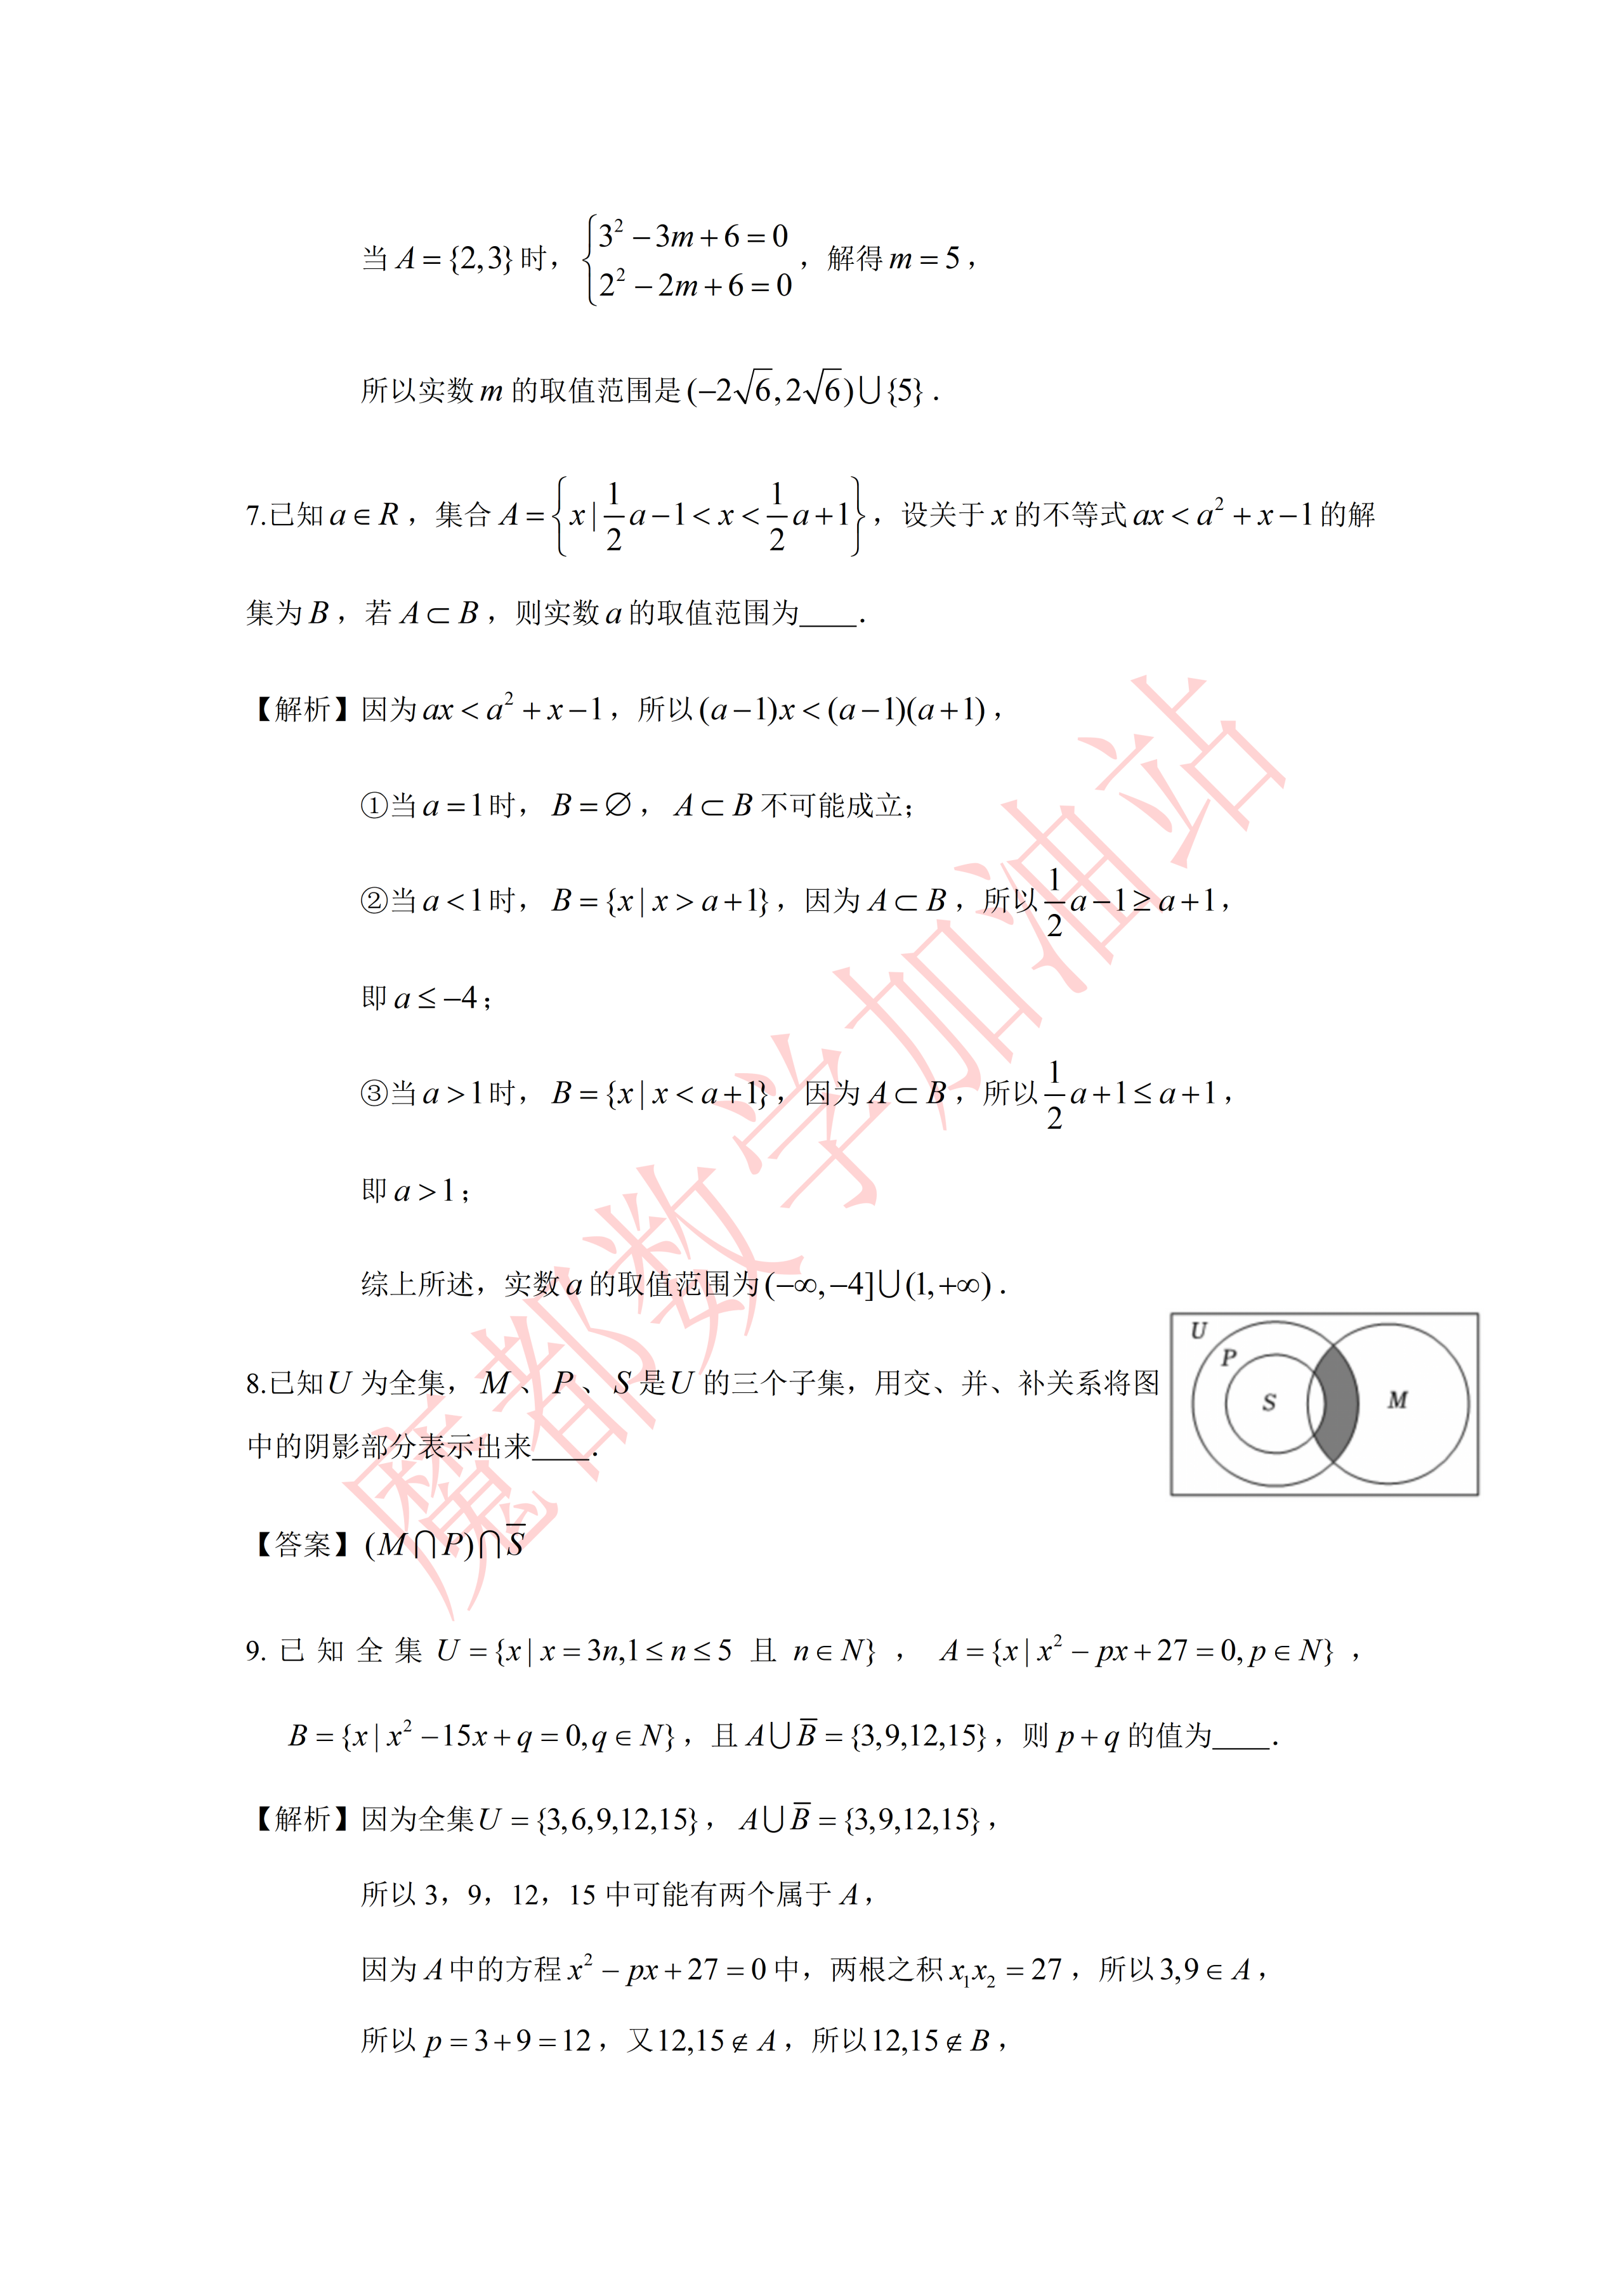
\includegraphics[width=.38\linewidth,trim=1835bp 1255bp 220bp 1565bp,clip]{../原图/高一49_华师大二附中_国庆作业1/02.png}
\end{center}

\ifanswer
\ans{$(M\cap P)\cap\overline S$}
\fi

\item 已知全集 $U=\{x\mid x=3n,1\leqslant n\leqslant5\text{ 且 }n\in\N\}$，$A=\{x\mid x^2-px+27=0,p\in\N\}$，$B=\{x\mid x^2-15x+q=0,q\in\N\}$，且 $A\cup\overline B=\{3,9,12,15\}$，则 $p+q$ 的值为\blankline[4.4em].

\ifanswer
\solbegin
\step{因为全集 $U=\{3,6,9,12,15\}$，$A\cup\overline B=\{3,9,12,15\}$，}
\step{所以 $3$、$9$、$12$、$15$ 中可能有两个属于 $A$，}
\step{因为 $A$ 中的方程 $x^2-px+27=0$ 中，两根之积 $x_1x_2=27$，所以 $3,9\in A$，}
\step{所以 $p=3+9=12$，又 $12,15\notin A$，所以 $12,15\notin B$，}
\step{因为 $B$ 中的方程 $x^2-15x+q=0$ 中，两根之和 $x_3+x_4=15$，所以 $6,9\in B$，}
\step{则 $q=6\times9=54$，所以 $p+q=66$.}
\solend
\fi

\item 已知集合 $A=\{x\mid x^2+(2a-3)x-3a=0,a\in\R,x\in\R\}$，集合 $B=\{x\mid x^2+(a-3)x+a^2-3a=0,a\in\R,x\in\R\}$，若 $A\neq B$，$A\cap B\neq\varnothing$，则 $A\cup B=$\blankline[4.4em].

\ifanswer
\solbegin
\step{设两个集合中的方程的公共解是 $b$，}
\step{由 $b^2+(2a-3)b-3a=b^2+(a-3)b+a^2-3a$，得 $ab=a^2$，}
\step{则 $a=0$ 或 $b=a$，}
\step{当 $a=0$ 时，不合题意，}
\step{当 $b=a$ 时，即两个方程的公共解为 $b=a$，}
\step{将 $b=a$ 代入方程，得 $a^2=2a$，$a=2$，}
\step{所以 $A=\{2,-3\}$，$B=\{-1,2\}$，所以 $A\cup B=\{-1,2,-3\}$.}
\solend
\fi

\item 已知一个有四个数字元素的集合 $S$，$S$ 的所有子集的元素和（空集的元素和认为是 $0$）的总和为 $16192$，则 $S$ 的元素之和等于\blankline[4.4em].

\ifanswer
\solbegin
\step{设 $S=\{a_1,a_2,a_3,a_4\}$，$S$ 的每个元素在所有子集中均出现 $2^3$ 次，}
\step{故 $(a_1+a_2+a_3+a_4)\cdot2^3=16192$，所以 $a_1+a_2+a_3+a_4=2024$，}
\step{故 $S$ 的元素之和等于 $2024$.}
\solend
\fi

\item 设 $P$ 为非空实数集满足：对任意给定的 $x,y\in P$（$x$、$y$ 可以相同），都有 $x+y\in P,x-y\in P,xy\in P$，则称 $P$ 为封闭集．关于封闭集有下列结论：

①集合 $P=\{-2,-1,0,1,2\}$ 为封闭集；

②集合 $P=\{x\mid x=2n,n\in\Z\}$ 为封闭集；

③若集合 $P_1$、$P_2$ 为封闭集，则 $P_1\cup P_2$ 为封闭集；

④若集合 $P$ 为封闭集，则一定有 $0\in P$；

⑤若集合 $P_1$、$P_2$ 为封闭集，则 $P_1\cap P_2$ 为封闭集.

其中正确结论的序号是\blankline[4.4em].

\ifanswer
\solbegin
\step{对于集合 $P=\{-2,-1,0,1,2\}$，取 $x=2$，$y=-2$，则 $x-y=2-(-2)=4\notin P$，}
\step{不满足封闭集的定义，所以①错误.}
\step{对于集合 $P=\{x\mid x=2n,n\in\Z\}$，设 $x=2n_1$，$y=2n_2$，$n_1,n_2\in\Z$.}
\step{$x+y=2n_1+2n_2=2(n_1+n_2)$，因为 $n_1+n_2\in\Z$，所以 $x+y\in P$.}
\step{$x-y=2n_1-2n_2=2(n_1-n_2)$，因为 $n_1-n_2\in\Z$，所以 $x-y\in P$.}
\step{$xy=2n_1\times2n_2=4n_1n_2=2(2n_1n_2)$，因为 $2n_1n_2\in\Z$，所以 $xy\in P$.}
\step{满足封闭集的定义，所以②正确.}
\step{令 $P_1=\{x\mid x=2n,n\in\Z\}$，$P_2=\{x\mid x=3n,n\in\Z\}$，都是封闭集.}
\step{$P_1\cup P_2$ 中，取 $x=2(x\in P_1)$，$y=3(y\in P_2)$，$x+y=5\notin P_1\cup P_2$，}
\step{不满足封闭集的定义，所以③错误.}
\step{因为对任意 $x\in P$，有 $x-x=0\in P$，}
\step{所以若集合 $P$ 为封闭集，则一定有 $0\in P$，所以④正确.}
\step{因为 $P_1$、$P_2$ 为封闭集，设 $x,y\in P_1\cap P_2$，则 $x,y\in P_1$ 且 $x,y\in P_2$.}
\step{因为 $P_1$ 是封闭集，所以 $x+y\in P_1,x-y\in P_1,xy\in P_1$.}
\step{因为 $P_2$ 是封闭集，所以 $x+y\in P_2,x-y\in P_2,xy\in P_2$.}
\step{所以 $x+y\in P_1\cap P_2,x-y\in P_1\cap P_2,xy\in P_1\cap P_2$，满足封闭集的定义，}
\step{所以⑤正确.}
\step{故正确的是②④⑤.}
\solend
\fi

\end{enumerate}

\bigsec{二、选择题}

\begin{enumerate}
\setcounter{enumi}{12}

\item 已知集合 $A=\{1,3,\sqrt m\}$，$B=\{1,m\}$，$B\subseteq A$，则 $m=$\mbox{（\quad）}

\keepwithprev
A. $0$ 或 $\sqrt3$\qquad B. $0$ 或 $3$

C. $1$ 或 $\sqrt3$\qquad D. $1$ 或 $3$

\ifanswer
\solbegin
\step{因为集合 $A=\{1,3,\sqrt m\}$，$B=\{1,m\}$，$B\subseteq A$，所以 $m=3$ 或 $m=\sqrt m$，}
\step{若 $m=3$，$A=\{1,3,\sqrt3\}$，$B=\{1,3\}$，满足 $B\subseteq A$，}
\step{若 $m=\sqrt m$，解得 $m=1$ 或 $m=0$，}
\step{①若 $m=0$，则 $A=\{1,3,0\}$，$B=\{1,0\}$，满足 $B\subseteq A$.}
\step{②若 $m=1$，则 $A$、$B$ 不满足集合中元素的互异性，舍去.}
\step{综上，$m=0$ 或 $m=3$．故选 $B$.}
\solend
\fi

\needvspace{10\baselineskip}

\item 设集合 $A$、$B$、$C$、$D$ 是全集 $X$ 的子集，$A\cap B\neq\varnothing$，$A\cap C\neq\varnothing$，则下列选项中正确的是\mbox{（\quad）}

\keepwithprev
A. 如果 $D\subset B$ 或 $D\subset C$，则 $D\cap A\neq\varnothing$

B. 如果 $D\subset A$，则 $\overline D\cap B\neq\varnothing$，$\overline D\cap C\neq\varnothing$

C. 如果 $A\subset D$，则 $\overline D\cap B=\varnothing$，$\overline D\cap C=\varnothing$

D. 上述各项都不正确

\ifanswer
\solbegin
\step{用韦恩图表示每个选项：}
\begin{center}
% 原图第 5 页解析配图（三联韦恩图）直接裁取（原卷排于选项 C、D 右侧）。
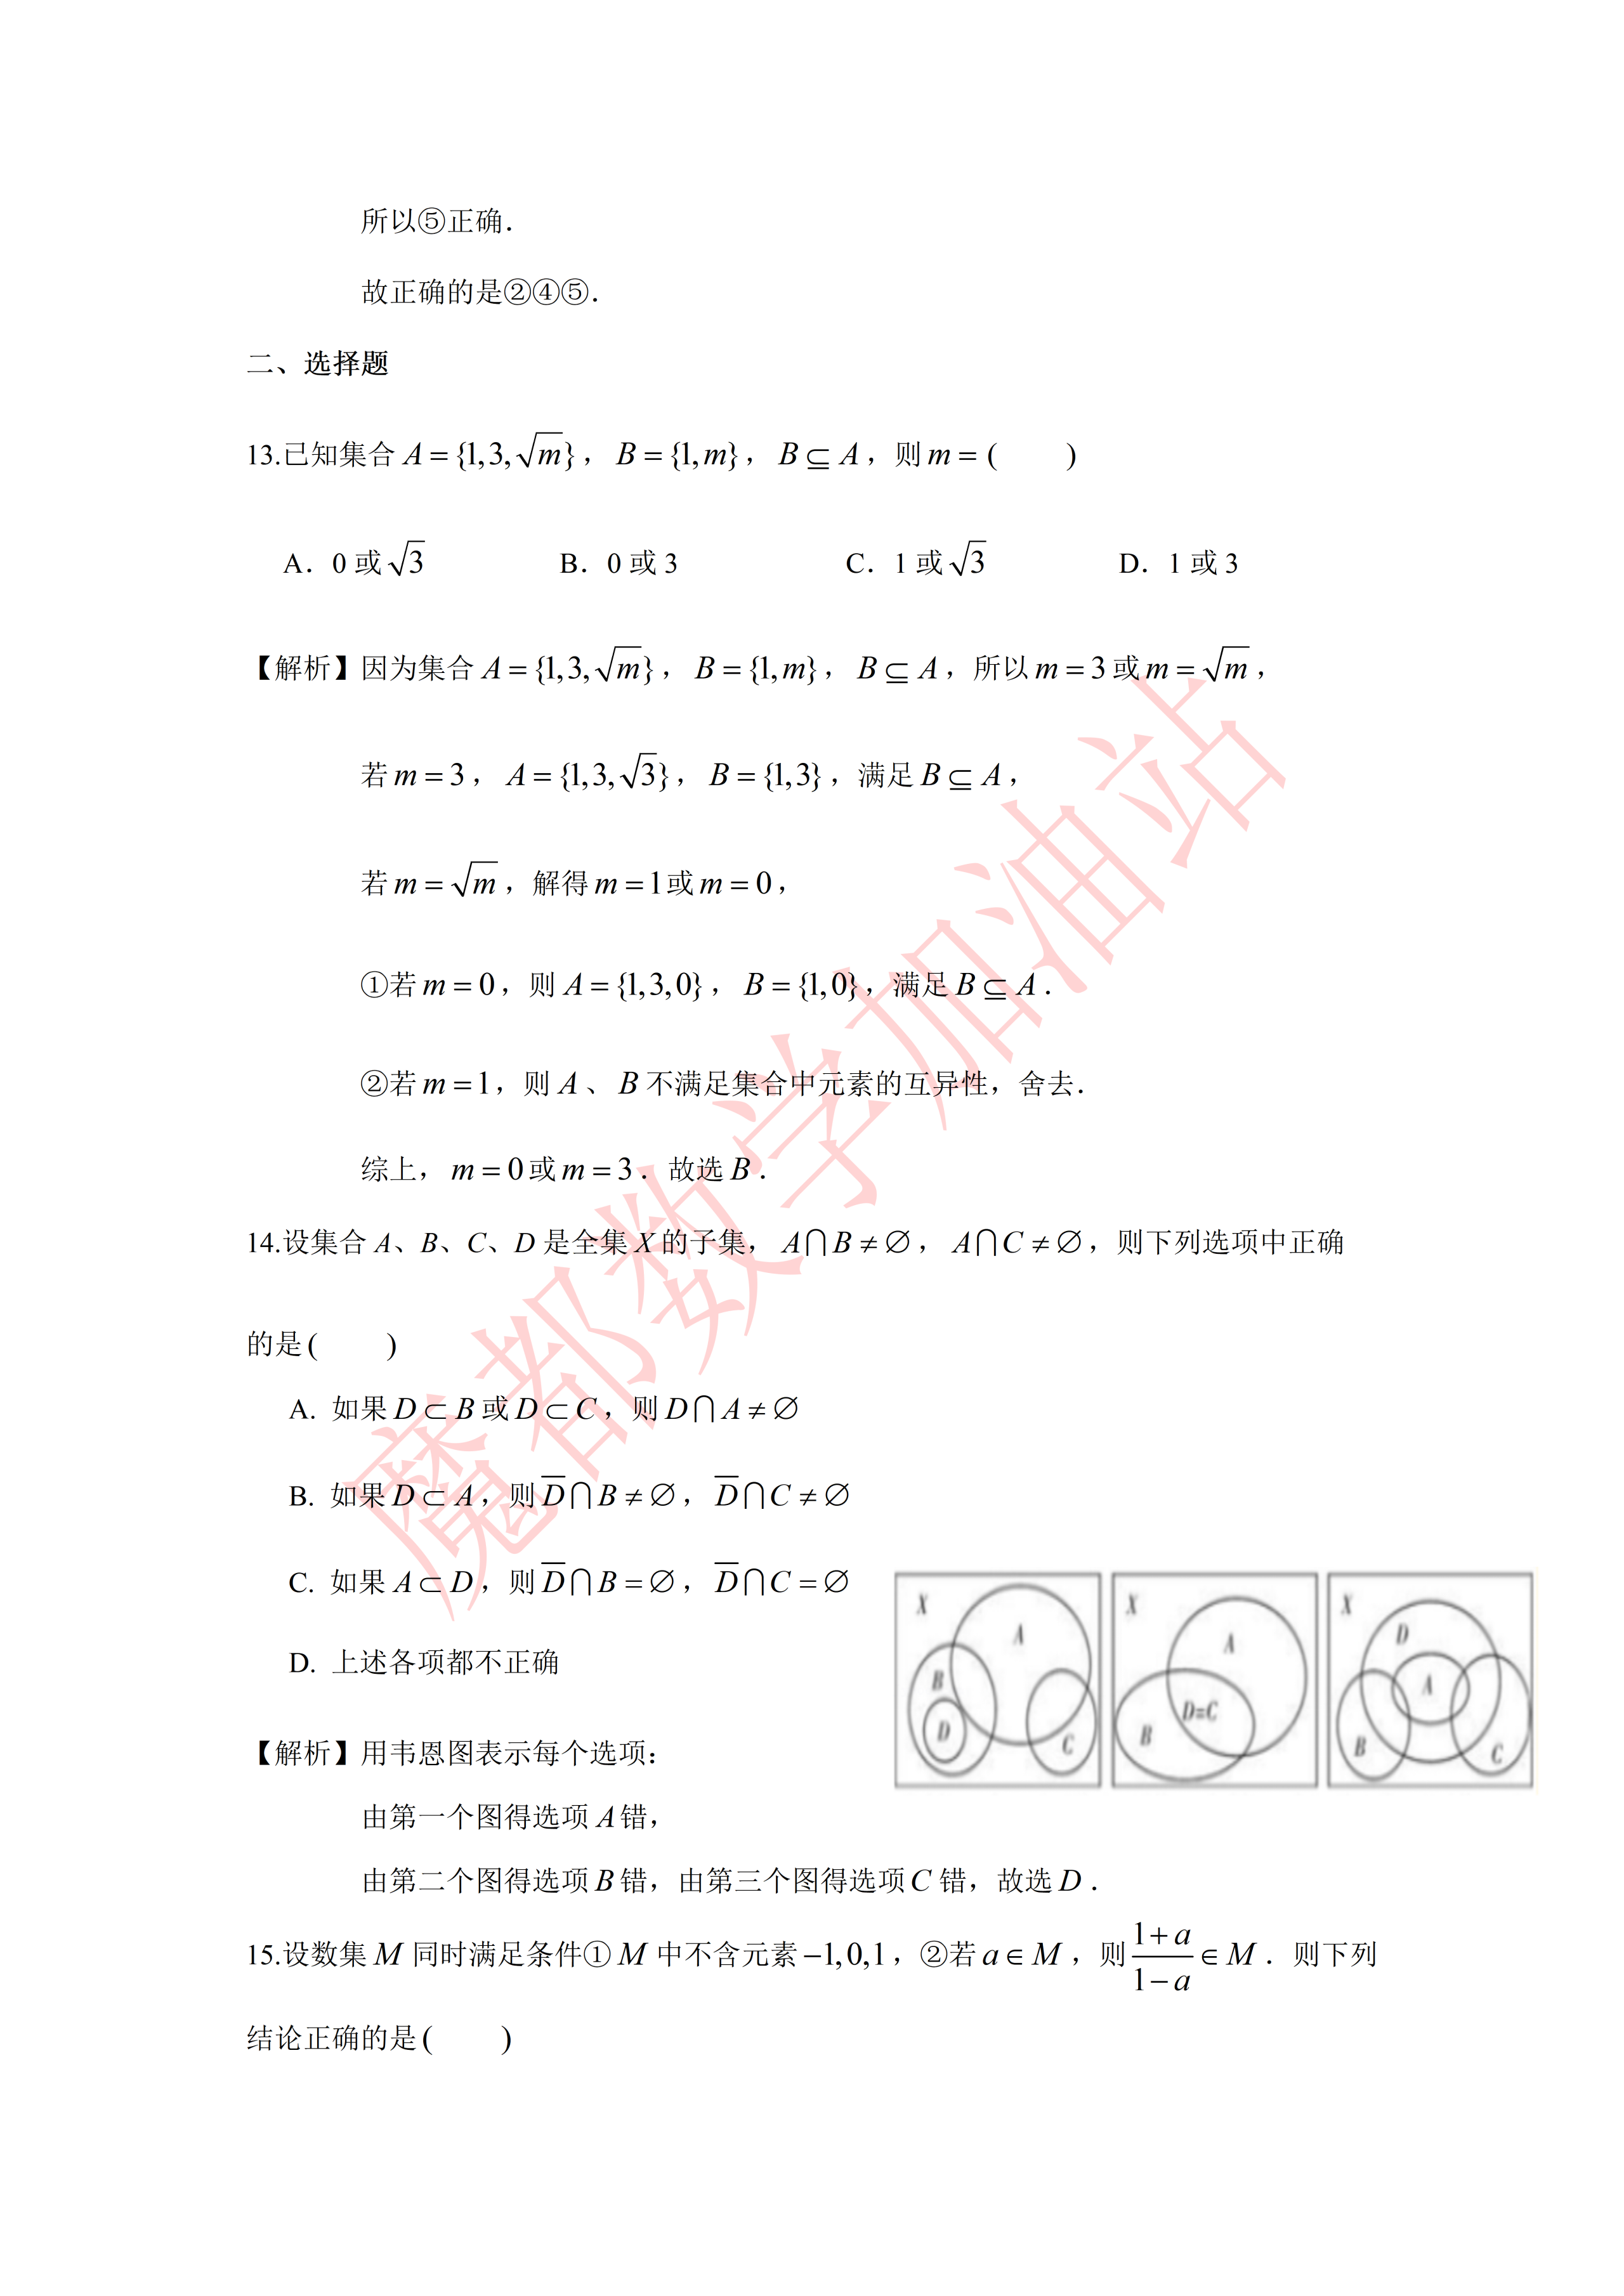
\includegraphics[width=.75\linewidth,trim=1400bp 790bp 135bp 1155bp,clip]{../原图/高一49_华师大二附中_国庆作业1/05.png}
\end{center}
\step{由第一个图得选项 $A$ 错，}
\step{由第二个图得选项 $B$ 错，由第三个图得选项 $C$ 错，故选 $D$.}
\solend
\fi

\item 设数集 $M$ 同时满足条件①$M$ 中不含元素 $-1$、$0$、$1$，②若 $a\in M$，则 $\dfrac{1+a}{1-a}\in M$．则下列结论正确的是\mbox{（\quad）}

\keepwithprev
A. 集合 $M$ 中至多有 $2$ 个元素\qquad B. 集合 $M$ 中至多有 $3$ 个元素

C. 集合 $M$ 中有且仅有 $4$ 个元素\qquad D. 集合 $M$ 中有无穷多个元素

\ifanswer
\solbegin
\step{若集合只含有一个元素，则 $\dfrac{1+a}{1-a}=a$，即 $1+a=a-a^2$，即 $-a^2=1$，不成立.}
\step{当 $a=3$ 时，$\dfrac{1+3}{1-3}=-2\in M$，所以 $\dfrac{1-2}{1+2}=-\dfrac13\in M$，所以 $\dfrac{1-\frac13}{1+\frac13}=\dfrac12\in M$，}
\step{所以 $\dfrac{1+\frac12}{1-\frac12}=3$，开始重复了，所以 $M=\left\{3,-2,-\dfrac13,\dfrac12\right\}$；}
\step{当 $a=2$ 时，$\dfrac{1+2}{1-2}=-3\in M$，所以 $\dfrac{1-3}{1+3}=-\dfrac12\in M$，所以 $\dfrac{1-\frac12}{1+\frac12}=\dfrac13\in M$，}
\step{所以 $\dfrac{1+\frac13}{1-\frac13}=2$，开始重复了，所以 $M=\left\{2,-3,-\dfrac12,-\dfrac13\right\}$，}
\step{此时也只要四个元素；}
\step{当 $a=\dfrac34\in M$，则 $7\in M$，若 $7\in M$，则 $-\dfrac43\in M$，}
\step{若 $-\dfrac43\in M$，则 $-\dfrac17\in M$，若 $-\dfrac17\in M$，有 $\dfrac34\in M$，}
\step{由归纳推理得，集合 $M$ 中有且仅有 $4$ 个元素．故选 $C$.}
\solend
\fi

\item 已知集合 $M=\{x\mid x\in\N,0<x\leqslant15\}$，$A_1$、$A_2$、$A_3$ 满足：①$A_1\cup A_2\cup A_3=M$；②每个集合都恰有 $5$ 个元素．集合 $A_i$（$i=1,2,3$）中最大元素与最小元素之和称为 $A_i$ 的特征数，记为 $X_i$（$i=1,2,3$），则 $X_1+X_2+X_3$ 的值不可能为\mbox{（\quad）}

\keepwithprev
A. $37$\qquad B. $39$\qquad C. $48$\qquad D. $57$

\ifanswer
\solbegin
\step{因为集合 $M=\{x\mid x\in\N,0<x\leqslant15\}=\{1,2,3,\cdots,15\}$，}
\step{又因为集合 $A_1$、$A_2$、$A_3$ 中，每个集合恰有 $5$ 个元素，}
\step{且 $A_1\cup A_2\cup A_3=M$ 有 $15$ 个元素，所以集合 $A_1$、$A_2$、$A_3$ 中没有重复元素，}
\step{因为 $1$ 是集合 $M$ 中数值最小的元素，$15$ 是集合 $M$ 中数值最大的元素，}
\step{所以在 $A_i$ 的特征数构成中，必有 $1$ 和 $15$，不妨设 $1\in A_1$，$15\in A_1$，}
\step{要使 $X_1+X_2+X_3$ 最大，则应该在集合 $A_1$ 中首先放置数值较小的元素，}
\step{即 $A_1=\{1,2,3,4,15\}$，所以 $5$ 与 $14$ 是剩下元素中数值最小或最大的元素，}
\step{同理，不妨设 $5\in A_2$，$14\in A_2$，接着在 $A_2$ 中再次放置数值较小的元素，}
\step{即 $A_2=\{5,6,7,8,14\}$，则 $A_3=\{9,10,11,12,13\}$，}
\step{此时 $X_1+X_2+X_3$ 有最大值为 $1+15+5+14+9+13=57$，}
\step{即 $X_1+X_2+X_3\leqslant57$；}
\step{要使 $X_1+X_2+X_3$ 最小，则在集合 $A_1$ 中首先放置数值较大的元素，}
\step{即 $A_1=\{1,12,13,14,15\}$，所以 $2$ 与 $11$ 是剩下元素中数值最小或最大的元素，}
\step{同理，不妨设 $2\in A_2$，$11\in A_2$，接着在 $A_2$ 中再次放置数值较大的元素，}
\step{即 $A_2=\{2,8,9,10,11\}$，则 $A_3=\{3,4,5,6,7\}$，}
\step{此时 $X_1+X_2+X_3$ 有最小值为 $1+15+2+11+3+7=39$，}
\step{即 $X_1+X_2+X_3\geqslant39$，}
\step{综上，$39\leqslant X_1+X_2+X_3\leqslant57$，故选 $A$.}
\solend
\fi

\end{enumerate}

\bigsec{三、解答题}

\begin{enumerate}
\setcounter{enumi}{16}

\item 已知全集为 $\R$，集合 $A=\{x\mid y=\sqrt{(2+x)(4-x)}\}$，$B=\{x\mid-1<x<m+1\}$.

\begin{enumerate}[label=(\arabic*)]
\item 若 $m=4$，求 $A\cup B$、$\overline A\cap B$；
\item 若 $B\subseteq A$，求实数 $m$ 的取值范围.
\end{enumerate}

\ifanswer
\solbegin
\stepm{(1)}{集合 $A=\{x\mid y=\sqrt{(2+x)(4-x)}\}=\{x\mid-2\leqslant x\leqslant4\}$，}
\step{当 $m=4$ 时，$B=\{x\mid-1<x<5\}$.}
\step{所以 $A\cup B=[-2,5)$，$\overline A=\{x\mid x<-2\text{ 或 }x>4\}$，$\overline A\cap B=(4,5)$.}
\stepm{(2)}{因为 $B\subseteq A$，}
% 原卷如此，照录未改（第 17 题(2)解析两处"当 C=∅／当 C≠∅"应为 B，本卷并无集合 C）
\step{当 $C=\varnothing$ 时，$m\leqslant-2$，$B\subseteq A$ 成立；}
\step{当 $C\neq\varnothing$ 时，$m>-2$，$-1<m+1\leqslant4$，解得 $-2<m\leqslant3$，}
\step{综上，$m\leqslant3$，所以实数 $m$ 的取值范围是 $(-\infty,3]$.}
\solend
\fi

\ansspace[6]

\item 用反证法证明：若 $a$、$b$、$c\in\R$，且 $x=a^2-2b+1$，$y=b^2-2c+1$，$z=c^2-2a+1$，则 $x$、$y$、$z$ 中至少有一个不小于 $0$.

\ifanswer
\solbegin
\step{假设 $x$、$y$、$z$ 均小于 $0$，即 $x=a^2-2b+1<0$①，$y=b^2-2c+1<0$②，}
\step{$z=c^2-2a+1<0$③，①$+$②$+$③得 $x+y+z=(a-1)^2+(b-1)^2+(c-1)^2<0$，}
\step{这与 $(a-1)^2+(b-1)^2+(c-1)^2\geqslant0$ 矛盾，则假设不成立，}
\step{所以 $x$、$y$、$z$ 中至少有一个不小于 $0$，得证.}
\solend
\fi

\ansspace[5]

\item 已知全集为 $\R$，实数 $a$、$b$ 满足 $a\neq b$，集合 $M=\{x\mid x^2-3x-4\leqslant0\}$，集合 $A=\{x\mid(x+a)(x+b)>0\}$，集合 $B=\{x\mid x^2+(a-2)x-2a>0\}$.

\begin{enumerate}[label=(\arabic*)]
\item 若 $\overline A=M$，求 $a$、$b$ 的值；
\item 若 $a>b>-1$，求 $A\cap B$；
\item 若 $a^2+a\in\overline B$，求 $a$ 的取值范围.
\end{enumerate}

\ifanswer
\solbegin
\stepm{(1)}{$M=\{x\mid x^2-3x-4\leqslant0\}=\{x\mid-1\leqslant x\leqslant4\}$，$A=\{x\mid(x+a)(x+b)\leqslant0\}$，}
\step{因为 $\overline A=M$，所以 $a=1$，$b=-4$ 或 $a=-4$，$b=1$.}
\stepm{(2)}{因为 $a>b>-1$，所以 $-a<-b<1$，所以 $A=\{x\mid x<-a\text{ 或 }x>-b\}$，}
\step{因为 $B=\{x\mid x^2+(a-2)x-2a>0\}=\{x\mid x<-a\text{ 或 }x>2\}$，}
\step{所以 $A\cap B=\{x\mid x<-a\text{ 或 }x>2\}$，}
\stepm{(3)}{$\overline B=\{x\mid(x-2)(x+a)\leqslant0\}$，}
% 原卷如此，照录未改（第 19 题(3)此处"a(a-1)((a-2)^2≤0"括号不配对；且由左式展开应为
% a(a-1)(a+2)^2≤0，与下句"解得 a=2 …[0,1]∪{2}"按 (a-2)^2 方自洽，见文件头清单第 2 条）
\step{由 $a^2+a\in\overline B$，得 $(a^2+a-2)(a^2+2a)\leqslant0\Leftrightarrow a(a-1)((a-2)^2\leqslant0$，}
\step{解得 $a=2$ 或 $0\leqslant a\leqslant1$，故 $a$ 的取值范围是 $[0,1]\cup\{2\}$.}
\solend
\fi

\ansspace[7]

\item 设数集 $A$ 由实数构成，若 $x\in A$（$x\neq1$ 且 $x\neq0$），则 $\dfrac{1}{1-x}\in A$.

\begin{enumerate}[label=(\arabic*)]
\item 若 $2\in A$，则 $A$ 中至少还有几个元素；
\item 集合 $A$ 是否为双元素集合？请说明理由；
\item 若 $A$ 中元素个数不超过 $8$ 个，所有元素的和为 $\dfrac{14}{3}$，且 $A$ 中有一个元素的平方等于所有元素的积，求集合 $A$.
\end{enumerate}

\ifanswer
\solbegin
\stepm{(1)}{若 $x\in A$，则 $\dfrac{1}{1-x}\in A$，又 $2\in A$，所以 $\dfrac{1}{1-2}=-1\in A$，}
\step{所以 $\dfrac{1}{1-(-1)}=\dfrac12\in A$，所以 $\dfrac{1}{1-\frac12}=2\in A$，}
% 原卷如此，照录未改（第 20 题(1)解析末句"2 个几个元素"衍一"几个"）
\step{所以 $A$ 中至少还有 $2$ 个几个元素；}
\stepm{(2)}{若 $x\in A$（$x\neq1$ 且 $x\neq0$），则 $\dfrac{1}{1-x}\in A$，}
\step{则 $\dfrac{1}{1-\frac{1}{1-x}}=\dfrac{1-x}{-x}\in A$，则 $\dfrac{1}{1-\frac{1-x}{-x}}=x\in A$}
\step{若 $A$ 为双元素集，则 $x=\dfrac{1}{1-x}$ 或 $x=\dfrac{1-x}{-x}$ 或 $\dfrac{1}{1-x}=\dfrac{1-x}{-x}$，均无解，}
\step{所以 $A$ 不可能为双元素集；}
\stepm{(3)}{由 $x\in A$，$\dfrac{1}{1-x}\in A$，得 $\dfrac{1}{1-\frac{1}{1-x}}=\dfrac{x-1}{x}\in A$，得 $\dfrac{1}{1-\frac{x-1}{x}}=x\in A$，}
\step{所以 $\left\{x,\dfrac{1}{1-x},\dfrac{x-1}{x}\right\}\subseteq A$，而 $x\cdot\dfrac{1}{1-x}\cdot\dfrac{x-1}{x}=-1$，}
\step{$A$ 中元素个数为 $3$ 的倍数，则 $A$ 中元素只有 $6$ 个，}
\step{因为 $A$ 中有一个元素的平方等于所有元素的积，}
\step{不妨设 $x^2=1$，解得 $x=-1$ 或 $x=1$（舍），则 $-1$、$\dfrac12$、$2\in A$，}
\step{所以 $-1+\dfrac12+2+m+\dfrac{1}{1-m}+\dfrac{m-1}{m}=\dfrac{14}{3}$，解得 $m=-\dfrac12$ 或 $m=3$ 或 $m=\dfrac23$，}
\step{所以 $A=\left\{\dfrac12,2,-1,-\dfrac12,3,\dfrac23\right\}$.}
\solend
\fi

\ansspace[9]

% 原卷如此，照录未改（第 21 题题干"21.求已知集合"之"求"字疑衍；"任意两个元素 a_i a_j"
% 疑脱逗号；"|a_i-a_j|≥1/30 则称"之前疑脱标点，见文件头清单第 4 条）
\item 求已知集合 $M=\left\{\dfrac{1}{k}\middle|1\leqslant k\leqslant100\text{ 且 }k\in\N^{*}\right\}$，$A=\{a_1,a_2,\cdots,a_n\}$，其中 $n\in\N^{*}$，且 $n\geqslant2$．若 $A\subseteq\N$，且对集合 $A$ 中的任意两个元素 $a_ia_j$，$i\neq j$ 都有 $|a_i-a_j|\geqslant\dfrac{1}{30}$ 则称集合 $A$ 有性质 $P$.

\begin{enumerate}[label=(\arabic*)]
\item 判断集合 $\left\{\dfrac13,\dfrac14,\dfrac15,\dfrac16,\dfrac17\right\}$ 是否具有性质 $P$；
\item 若集合 $A=\{a_1,a_2,\cdots,a_n\}$ 具有性质 $P$.

①求证：$a_i-a_j$ 的最大值大于等于 $\dfrac{n-1}{30}$；

②求 $A$ 的元素个数 $n$ 的最大值.
\end{enumerate}

\ifanswer
\solbegin
\stepm{(1)}{集合为 $\left\{\dfrac13,\dfrac14,\dfrac15,\dfrac16,\dfrac17\right\}$，又 $\dfrac16-\dfrac17=\dfrac{1}{42}<\dfrac{1}{30}$，所以该集合不具有性质 $P$；}
\stepm{(2)}{①因为集合 $A=\{a_1,a_2,\cdots,a_n\}$ 具有性质 $P$，}
\step{不妨设 $a_1<a_2<a_3<\cdots<a_n$，则 $a_i-a_j\geqslant\dfrac{1}{30}$（$i>j$），}
\step{所以 $a_n-a_1=(a_n-a_{n-1})+(a_{n-1}-a_{n-2})+\cdots+(a_2-a_1)\geqslant\dfrac{n-1}{30}$，}
\step{故 $a_i-a_j$ 的最大值大于等于 $\dfrac{n-1}{30}$；}
% 原卷如此，照录未改（第 21 题(2)②首行"a_2-a_1≥(n-1)/30"：由①同款推理只能得
% a_2-a_1≥1/30，见文件头清单第 5 条）
\step{②$A=\{a_1,a_2,\cdots,a_n\}$，不妨设 $a_1<a_2<a_3<\cdots<a_n$，}
\step{要使 $A$ 的元素个数 $n$ 最大，}
\step{则 $A$ 中的元素满足 $a_n=\dfrac{1}{k}$，$a_{n-1}=\dfrac{1}{k+1}$，$\cdots$，$a_1=\dfrac{1}{k+n-1}$（$k\in\N^{*}$），}
\step{又由①得 $a_2-a_1=\dfrac{1}{k+n-2}-\dfrac{1}{k+n-1}\geqslant\dfrac{n-1}{30}$，}
\step{所以 $(k+n-2)(k+n-1)\leqslant30$，又 $a_n-a_{n-1}=\dfrac{1}{k}-\dfrac{1}{k+1}\geqslant\dfrac{1}{30}$，}
\step{所以 $k(k+1)\leqslant30$，所以 $1\leqslant k\leqslant5$（$k\in\N^{*}$），}
\step{当 $k=5$ 时，由 $(k+n-2)(k+n-1)\leqslant30$，解得 $n\leqslant2$，$n\in\N^{*}$；}
\step{当 $k=4$ 时，由 $(k+n-2)(k+n-1)\leqslant30$，解得 $n\leqslant3$，$n\in\N^{*}$；}
\step{当 $k=3$ 时，由 $(k+n-2)(k+n-1)\leqslant30$，解得 $n\leqslant4$，$n\in\N^{*}$；}
\step{当 $k=2$ 时，由 $(k+n-2)(k+n-1)\leqslant30$，解得 $n\leqslant5$，$n\in\N^{*}$；}
\step{当 $k=1$ 时，由 $(k+n-2)(k+n-1)\leqslant30$，解得 $n\leqslant6$，$n\in\N^{*}$.}
\step{故 $A$ 的元素个数 $n$ 的最大值为 $6$，此时集合 $A=\left\{1,\dfrac12,\dfrac13,\cdots,\dfrac16\right\}$.}
\solend
\fi

\ansspace*[10]

\end{enumerate}

\end{document}
"
% 紧凑版：xelatex "\def\iscompact{1}% 高一49_华师大二附中_国庆作业1.tex
%   —— 高一上数学"2026-2027 年华师大二附中高一上国庆作业 1"（讲评版）
% 试卷版：xelatex 高一49_华师大二附中_国庆作业1.tex
% 答案版：xelatex "\def\isanswer{1}\input{高一49_华师大二附中_国庆作业1.tex}"
% 紧凑版：xelatex "\def\iscompact{1}\input{高一49_华师大二附中_国庆作业1.tex}"
%
% 原始材料：微信公众号"魔都数学加油站"文章，作者破晓，连载"27学年高一49"；
% 原文标题"27学年高一49——2026-2027年上海市华师大二附中高一上国庆作业1集合与逻辑、
% 等式与不等式的性质"；页面用 JS 渲染，未见明确发布日期（页内时间戳 ≈ 2026-10-05 21:37）；
% 原文链接：https://mp.weixin.qq.com/s/XxZTOBVQslK5cZm2_BbhOg。
% 正文为 11 张 PNG 页：第 01、03、04、06、07、08、09 页 4762×6735，
% 第 02、05、10、11 页 2560×3620，均按页序读取；粉色斜排"魔都数学加油站"为卷面水印，
% 与公众号页脚一并未录入。全卷 11 页均为试卷页，无二维码/宣传页。
%
% 题号与分节：原文自第 3 题起编，填空题 3—12、选择题 13—16、解答题 17—21，共 19 题。
% 讲评版：原卷每题下直接印【答案】或【解析】——只印【答案】的 3 题（第 3、5、8 题），
% 其余 16 题均只印【解析】；解析行数已逐题按印刷行照录（一条 \step＝原卷一个印刷行）。
%
% 卷首标题：照卷面印作"2026-2027 年华师大二附中高一上国庆作业 1"（公众号标题中的"上海市"
% 卷面没有，本稿照卷面），年份区间按全稿惯例排 en dash；副标题照卷面自印的
% "集合与逻辑单元综合检测"（原卷页首标题行下方即印此行，故不另按模块口径拟名）。
% 副标题依据：全卷 19 题均为集合与常用逻辑用语内容——集合类 15 题（6—17、19—21 中除
% 反证法题外），逻辑/命题类 3 题（第 3 题否定形式、第 4 题充要条件、第 5 题反证法假设），
% 反证法证明 1 题（第 18 题）；全卷无不等式求解题，公众号标题中"等式与不等式的性质"
% 与卷面实际内容不符。
%
% 与原卷的排版差异：
%   ① 原文从第 3 题起，填空题为 3—12、选择题为 13—16、解答题为 17—21，本稿保留原题号；
%   ② 原卷每题下直接印【答案】/【解析】，本稿按全稿惯例置于答案版；只印【解析】的题
%      不另提 \ans{}（照 高一36 口径），只印【答案】的题仅给 \ans{}；
%   ③ 原卷第 8 题韦恩图排在题干右侧、第 14 题三联韦恩图排在选项（C、D）右侧，
%      本稿分别移至题干下方、解析首步之后居中排，均直接裁取原图页（02.png、05.png）；
%   ④ 数集记号原卷排作斜体/加粗 R、N、Z，本稿统一为 \R、\N、\Z、\N^*；
%      填空横线按全稿惯例排为 \blankline[4.4em]。
%
% 原卷笔误/存疑清单（均照录未改，正文中该处有 % 注）：
%   1. 第 17 题(2)解析两处"当 C=∅／当 C≠∅"应为 B（本卷并无集合 C）；
%   2. 第 19 题(3)解析"a(a-1)((a-2)^2≤0"括号不配对（多一枚左括号）；且由
%      (a^2+a-2)(a^2+2a)≤0 展开应为 a(a-1)(a+2)^2≤0，与原卷结论"解得 a=2 …
%      [0,1]∪{2}"恰按 (a-2)^2 自洽——因式分解与原式不符，结论按 (a-2)^2 自洽，均照录；
%   3. 第 20 题(1)解析末句"至少还有 2 个几个元素"衍一"几个"；
%   4. 第 21 题题干"21.求已知集合"之"求"字疑衍；"任意两个元素 a_i a_j"疑脱逗号；
%      "≥1/30 则称"之前疑脱标点；
%   5. 第 21 题(2)②解析"a_2-a_1≥(n-1)/30"：由①同款推理只能得 a_2-a_1≥1/30，
%      原卷如此，照录未改（后续 (k+n-2)(k+n-1)≤30 即按该行推得）。
%
\documentclass[a4paper,11pt]{article}
\usepackage{common}

\begin{document}

\examtitlest[3]{2026--2027 年华师大二附中高一上国庆作业 1}{集合与逻辑单元综合检测}

\bigsec{一、填空题}

\begin{enumerate}
\setcounter{enumi}{2}

\item “若 $x^2-x-2\leqslant0$，则 $-1\leqslant x\leqslant2$”的否定形式为\blankline[4.4em].

\ifanswer
\ans{若 $x^2-x-2>0$，则 $x<-1$ 或 $x>2$}
\fi

\item 已知 $p:|x-3|<5$，$q:1-a<x<2a-3$，且 $p$ 是 $q$ 的充分非必要条件，则实数 $a$ 的取值范围是\blankline[4.4em].

\ifanswer
\solbegin
\step{由 $|x-3|<5$ 得 $-2<x<8$，}
\step{又 $p$ 是 $q$ 的充分不必要条件，所以 $(-2,8)\subset(1-a,2a-3)$，}
\step{即 $\begin{cases}-2\geqslant1-a\\ 8\leqslant2a-3\\ (2a-3)-(1-a)\neq8-(-2)\end{cases}$，解得 $a\geqslant\dfrac{11}{2}$，实数 $a$ 的取值范围是 $\left[\dfrac{11}{2},+\infty\right)$.}
\solend
\fi

\item 用反证法证明命题“设 $a$、$b\in\R$，则方程 $a_1x^2+b_1x+c_1=0$ 与 $a_2x^2+b_2x+c_2=0$ 至少有一个实根”时要做的假设是\blankline[4.4em].

\ifanswer
\ans{假设 $a$、$b\in\R$，方程 $a_1x^2+b_1x+c_1=0$ 与 $a_2x^2+b_2x+c_2=0$ 都没有实根}
\fi

\item 设集合 $A=\{x\mid x^2-mx+6=0,x\in\R\}$，且 $A\cap\{2,3\}=A$，则实数 $m$ 的取值范围是\blankline[4.4em].

\ifanswer
\solbegin
\step{由 $A\cap\{2,3\}=A$，得 $A\subseteq\{2,3\}$，}
\step{当 $A=\varnothing$ 时，$\Delta=m^2-24<0$，解得 $-2\sqrt6<m<2\sqrt6$；}
\step{当 $A=\{2\}$ 时，$\begin{cases}2^2-2m+6=0\\ \Delta=m^2-24=0\end{cases}$，无解；}
\step{当 $A=\{3\}$ 时，$\begin{cases}3^2-3m+6=0\\ \Delta=m^2-24=0\end{cases}$，无解；}
\step{当 $A=\{2,3\}$ 时，$\begin{cases}3^2-3m+6=0\\ 2^2-2m+6=0\end{cases}$，解得 $m=5$，}
\step{所以实数 $m$ 的取值范围是 $(-2\sqrt6,2\sqrt6)\cup\{5\}$.}
\solend
\fi

\item 已知 $a\in\R$，集合 $A=\left\{x\middle|\dfrac12a-1<x<\dfrac12a+1\right\}$，设关于 $x$ 的不等式 $ax<a^2+x-1$ 的解集为 $B$，若 $A\subset B$，则实数 $a$ 的取值范围为\blankline[4.4em].

\ifanswer
\solbegin
\step{因为 $ax<a^2+x-1$，所以 $(a-1)x<(a-1)(a+1)$，}
\step{①当 $a=1$ 时，$B=\varnothing$，$A\subset B$ 不可能成立；}
\step{②当 $a<1$ 时，$B=\{x\mid x>a+1\}$，因为 $A\subset B$，所以 $\dfrac12a-1\geqslant a+1$，}
\step{即 $a\leqslant-4$；}
\step{③当 $a>1$ 时，$B=\{x\mid x<a+1\}$，因为 $A\subset B$，所以 $\dfrac12a+1\leqslant a+1$，}
\step{即 $a>1$；}
\step{综上所述，实数 $a$ 的取值范围为 $(-\infty,-4]\cup(1,+\infty)$.}
\solend
\fi

\needvspace{8\baselineskip}

\item 已知 $U$ 为全集，$M$、$P$、$S$ 是 $U$ 的三个子集，用交、并、补关系将图中的阴影部分表示出来\blankline[4.4em].

\begin{center}
% 原图第 2 页题旁韦恩图直接裁取（原卷排于题干右侧）。
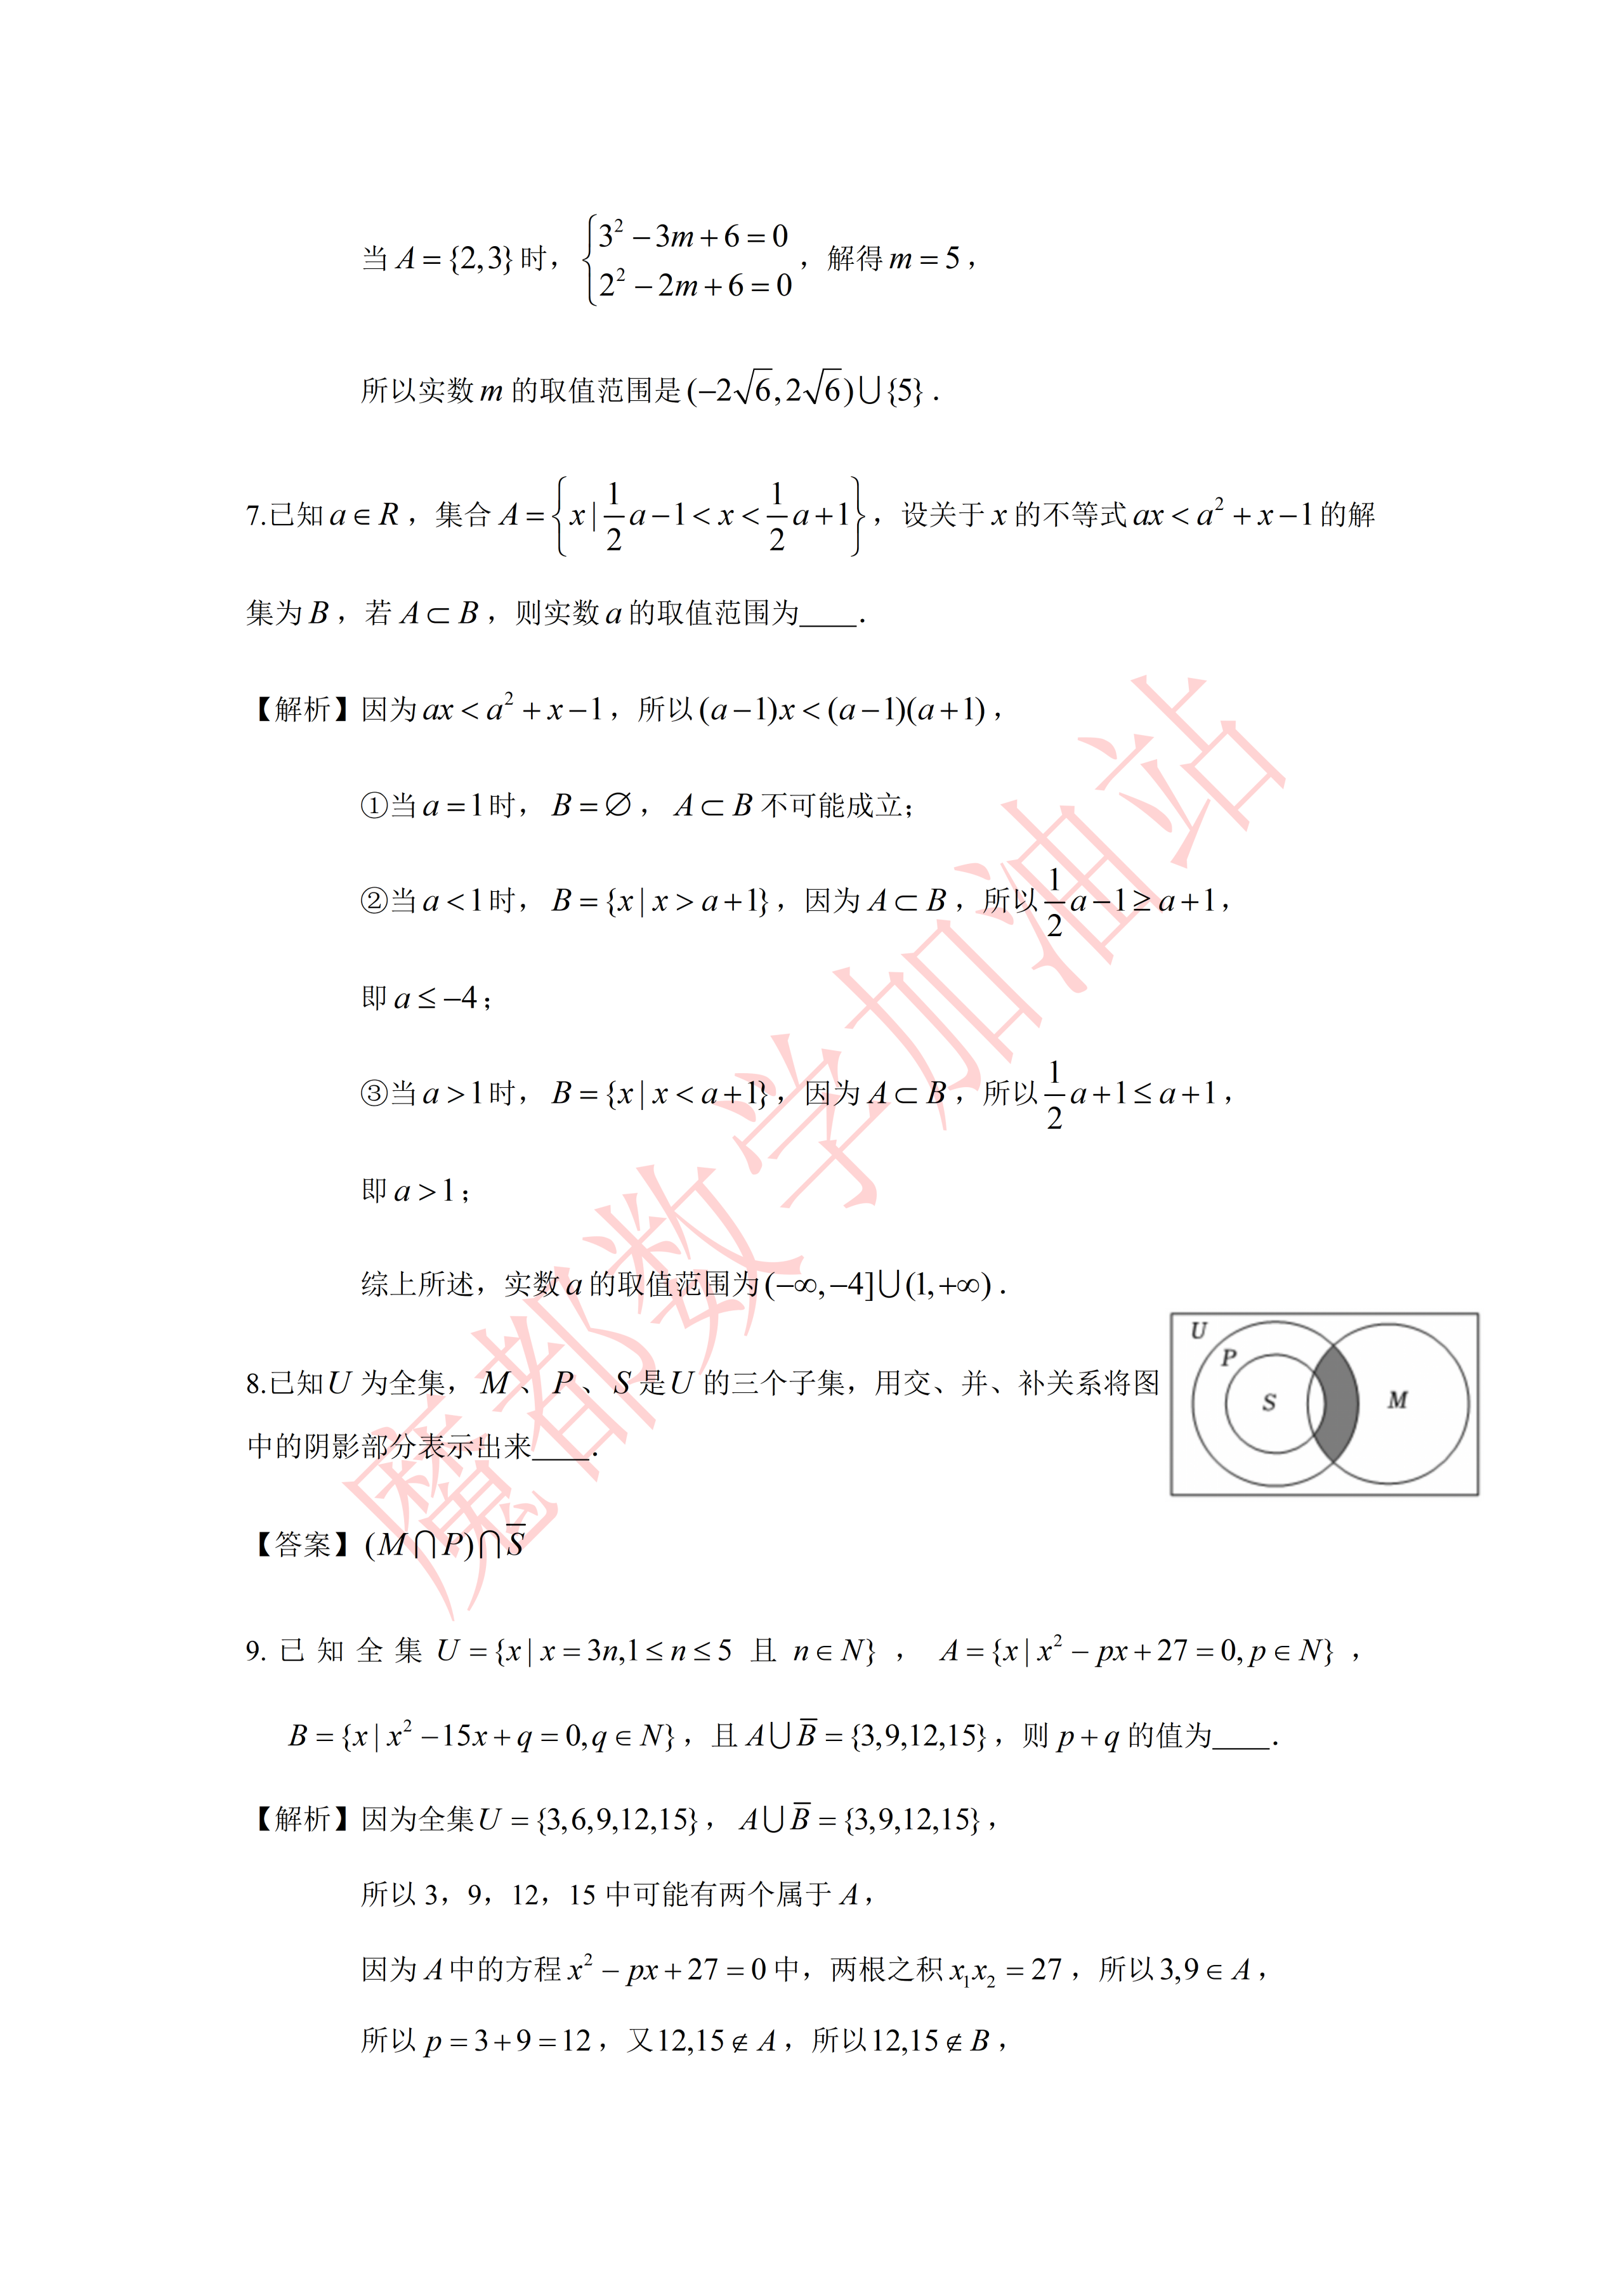
\includegraphics[width=.38\linewidth,trim=1835bp 1255bp 220bp 1565bp,clip]{../原图/高一49_华师大二附中_国庆作业1/02.png}
\end{center}

\ifanswer
\ans{$(M\cap P)\cap\overline S$}
\fi

\item 已知全集 $U=\{x\mid x=3n,1\leqslant n\leqslant5\text{ 且 }n\in\N\}$，$A=\{x\mid x^2-px+27=0,p\in\N\}$，$B=\{x\mid x^2-15x+q=0,q\in\N\}$，且 $A\cup\overline B=\{3,9,12,15\}$，则 $p+q$ 的值为\blankline[4.4em].

\ifanswer
\solbegin
\step{因为全集 $U=\{3,6,9,12,15\}$，$A\cup\overline B=\{3,9,12,15\}$，}
\step{所以 $3$、$9$、$12$、$15$ 中可能有两个属于 $A$，}
\step{因为 $A$ 中的方程 $x^2-px+27=0$ 中，两根之积 $x_1x_2=27$，所以 $3,9\in A$，}
\step{所以 $p=3+9=12$，又 $12,15\notin A$，所以 $12,15\notin B$，}
\step{因为 $B$ 中的方程 $x^2-15x+q=0$ 中，两根之和 $x_3+x_4=15$，所以 $6,9\in B$，}
\step{则 $q=6\times9=54$，所以 $p+q=66$.}
\solend
\fi

\item 已知集合 $A=\{x\mid x^2+(2a-3)x-3a=0,a\in\R,x\in\R\}$，集合 $B=\{x\mid x^2+(a-3)x+a^2-3a=0,a\in\R,x\in\R\}$，若 $A\neq B$，$A\cap B\neq\varnothing$，则 $A\cup B=$\blankline[4.4em].

\ifanswer
\solbegin
\step{设两个集合中的方程的公共解是 $b$，}
\step{由 $b^2+(2a-3)b-3a=b^2+(a-3)b+a^2-3a$，得 $ab=a^2$，}
\step{则 $a=0$ 或 $b=a$，}
\step{当 $a=0$ 时，不合题意，}
\step{当 $b=a$ 时，即两个方程的公共解为 $b=a$，}
\step{将 $b=a$ 代入方程，得 $a^2=2a$，$a=2$，}
\step{所以 $A=\{2,-3\}$，$B=\{-1,2\}$，所以 $A\cup B=\{-1,2,-3\}$.}
\solend
\fi

\item 已知一个有四个数字元素的集合 $S$，$S$ 的所有子集的元素和（空集的元素和认为是 $0$）的总和为 $16192$，则 $S$ 的元素之和等于\blankline[4.4em].

\ifanswer
\solbegin
\step{设 $S=\{a_1,a_2,a_3,a_4\}$，$S$ 的每个元素在所有子集中均出现 $2^3$ 次，}
\step{故 $(a_1+a_2+a_3+a_4)\cdot2^3=16192$，所以 $a_1+a_2+a_3+a_4=2024$，}
\step{故 $S$ 的元素之和等于 $2024$.}
\solend
\fi

\item 设 $P$ 为非空实数集满足：对任意给定的 $x,y\in P$（$x$、$y$ 可以相同），都有 $x+y\in P,x-y\in P,xy\in P$，则称 $P$ 为封闭集．关于封闭集有下列结论：

①集合 $P=\{-2,-1,0,1,2\}$ 为封闭集；

②集合 $P=\{x\mid x=2n,n\in\Z\}$ 为封闭集；

③若集合 $P_1$、$P_2$ 为封闭集，则 $P_1\cup P_2$ 为封闭集；

④若集合 $P$ 为封闭集，则一定有 $0\in P$；

⑤若集合 $P_1$、$P_2$ 为封闭集，则 $P_1\cap P_2$ 为封闭集.

其中正确结论的序号是\blankline[4.4em].

\ifanswer
\solbegin
\step{对于集合 $P=\{-2,-1,0,1,2\}$，取 $x=2$，$y=-2$，则 $x-y=2-(-2)=4\notin P$，}
\step{不满足封闭集的定义，所以①错误.}
\step{对于集合 $P=\{x\mid x=2n,n\in\Z\}$，设 $x=2n_1$，$y=2n_2$，$n_1,n_2\in\Z$.}
\step{$x+y=2n_1+2n_2=2(n_1+n_2)$，因为 $n_1+n_2\in\Z$，所以 $x+y\in P$.}
\step{$x-y=2n_1-2n_2=2(n_1-n_2)$，因为 $n_1-n_2\in\Z$，所以 $x-y\in P$.}
\step{$xy=2n_1\times2n_2=4n_1n_2=2(2n_1n_2)$，因为 $2n_1n_2\in\Z$，所以 $xy\in P$.}
\step{满足封闭集的定义，所以②正确.}
\step{令 $P_1=\{x\mid x=2n,n\in\Z\}$，$P_2=\{x\mid x=3n,n\in\Z\}$，都是封闭集.}
\step{$P_1\cup P_2$ 中，取 $x=2(x\in P_1)$，$y=3(y\in P_2)$，$x+y=5\notin P_1\cup P_2$，}
\step{不满足封闭集的定义，所以③错误.}
\step{因为对任意 $x\in P$，有 $x-x=0\in P$，}
\step{所以若集合 $P$ 为封闭集，则一定有 $0\in P$，所以④正确.}
\step{因为 $P_1$、$P_2$ 为封闭集，设 $x,y\in P_1\cap P_2$，则 $x,y\in P_1$ 且 $x,y\in P_2$.}
\step{因为 $P_1$ 是封闭集，所以 $x+y\in P_1,x-y\in P_1,xy\in P_1$.}
\step{因为 $P_2$ 是封闭集，所以 $x+y\in P_2,x-y\in P_2,xy\in P_2$.}
\step{所以 $x+y\in P_1\cap P_2,x-y\in P_1\cap P_2,xy\in P_1\cap P_2$，满足封闭集的定义，}
\step{所以⑤正确.}
\step{故正确的是②④⑤.}
\solend
\fi

\end{enumerate}

\bigsec{二、选择题}

\begin{enumerate}
\setcounter{enumi}{12}

\item 已知集合 $A=\{1,3,\sqrt m\}$，$B=\{1,m\}$，$B\subseteq A$，则 $m=$\mbox{（\quad）}

\keepwithprev
A. $0$ 或 $\sqrt3$\qquad B. $0$ 或 $3$

C. $1$ 或 $\sqrt3$\qquad D. $1$ 或 $3$

\ifanswer
\solbegin
\step{因为集合 $A=\{1,3,\sqrt m\}$，$B=\{1,m\}$，$B\subseteq A$，所以 $m=3$ 或 $m=\sqrt m$，}
\step{若 $m=3$，$A=\{1,3,\sqrt3\}$，$B=\{1,3\}$，满足 $B\subseteq A$，}
\step{若 $m=\sqrt m$，解得 $m=1$ 或 $m=0$，}
\step{①若 $m=0$，则 $A=\{1,3,0\}$，$B=\{1,0\}$，满足 $B\subseteq A$.}
\step{②若 $m=1$，则 $A$、$B$ 不满足集合中元素的互异性，舍去.}
\step{综上，$m=0$ 或 $m=3$．故选 $B$.}
\solend
\fi

\needvspace{10\baselineskip}

\item 设集合 $A$、$B$、$C$、$D$ 是全集 $X$ 的子集，$A\cap B\neq\varnothing$，$A\cap C\neq\varnothing$，则下列选项中正确的是\mbox{（\quad）}

\keepwithprev
A. 如果 $D\subset B$ 或 $D\subset C$，则 $D\cap A\neq\varnothing$

B. 如果 $D\subset A$，则 $\overline D\cap B\neq\varnothing$，$\overline D\cap C\neq\varnothing$

C. 如果 $A\subset D$，则 $\overline D\cap B=\varnothing$，$\overline D\cap C=\varnothing$

D. 上述各项都不正确

\ifanswer
\solbegin
\step{用韦恩图表示每个选项：}
\begin{center}
% 原图第 5 页解析配图（三联韦恩图）直接裁取（原卷排于选项 C、D 右侧）。
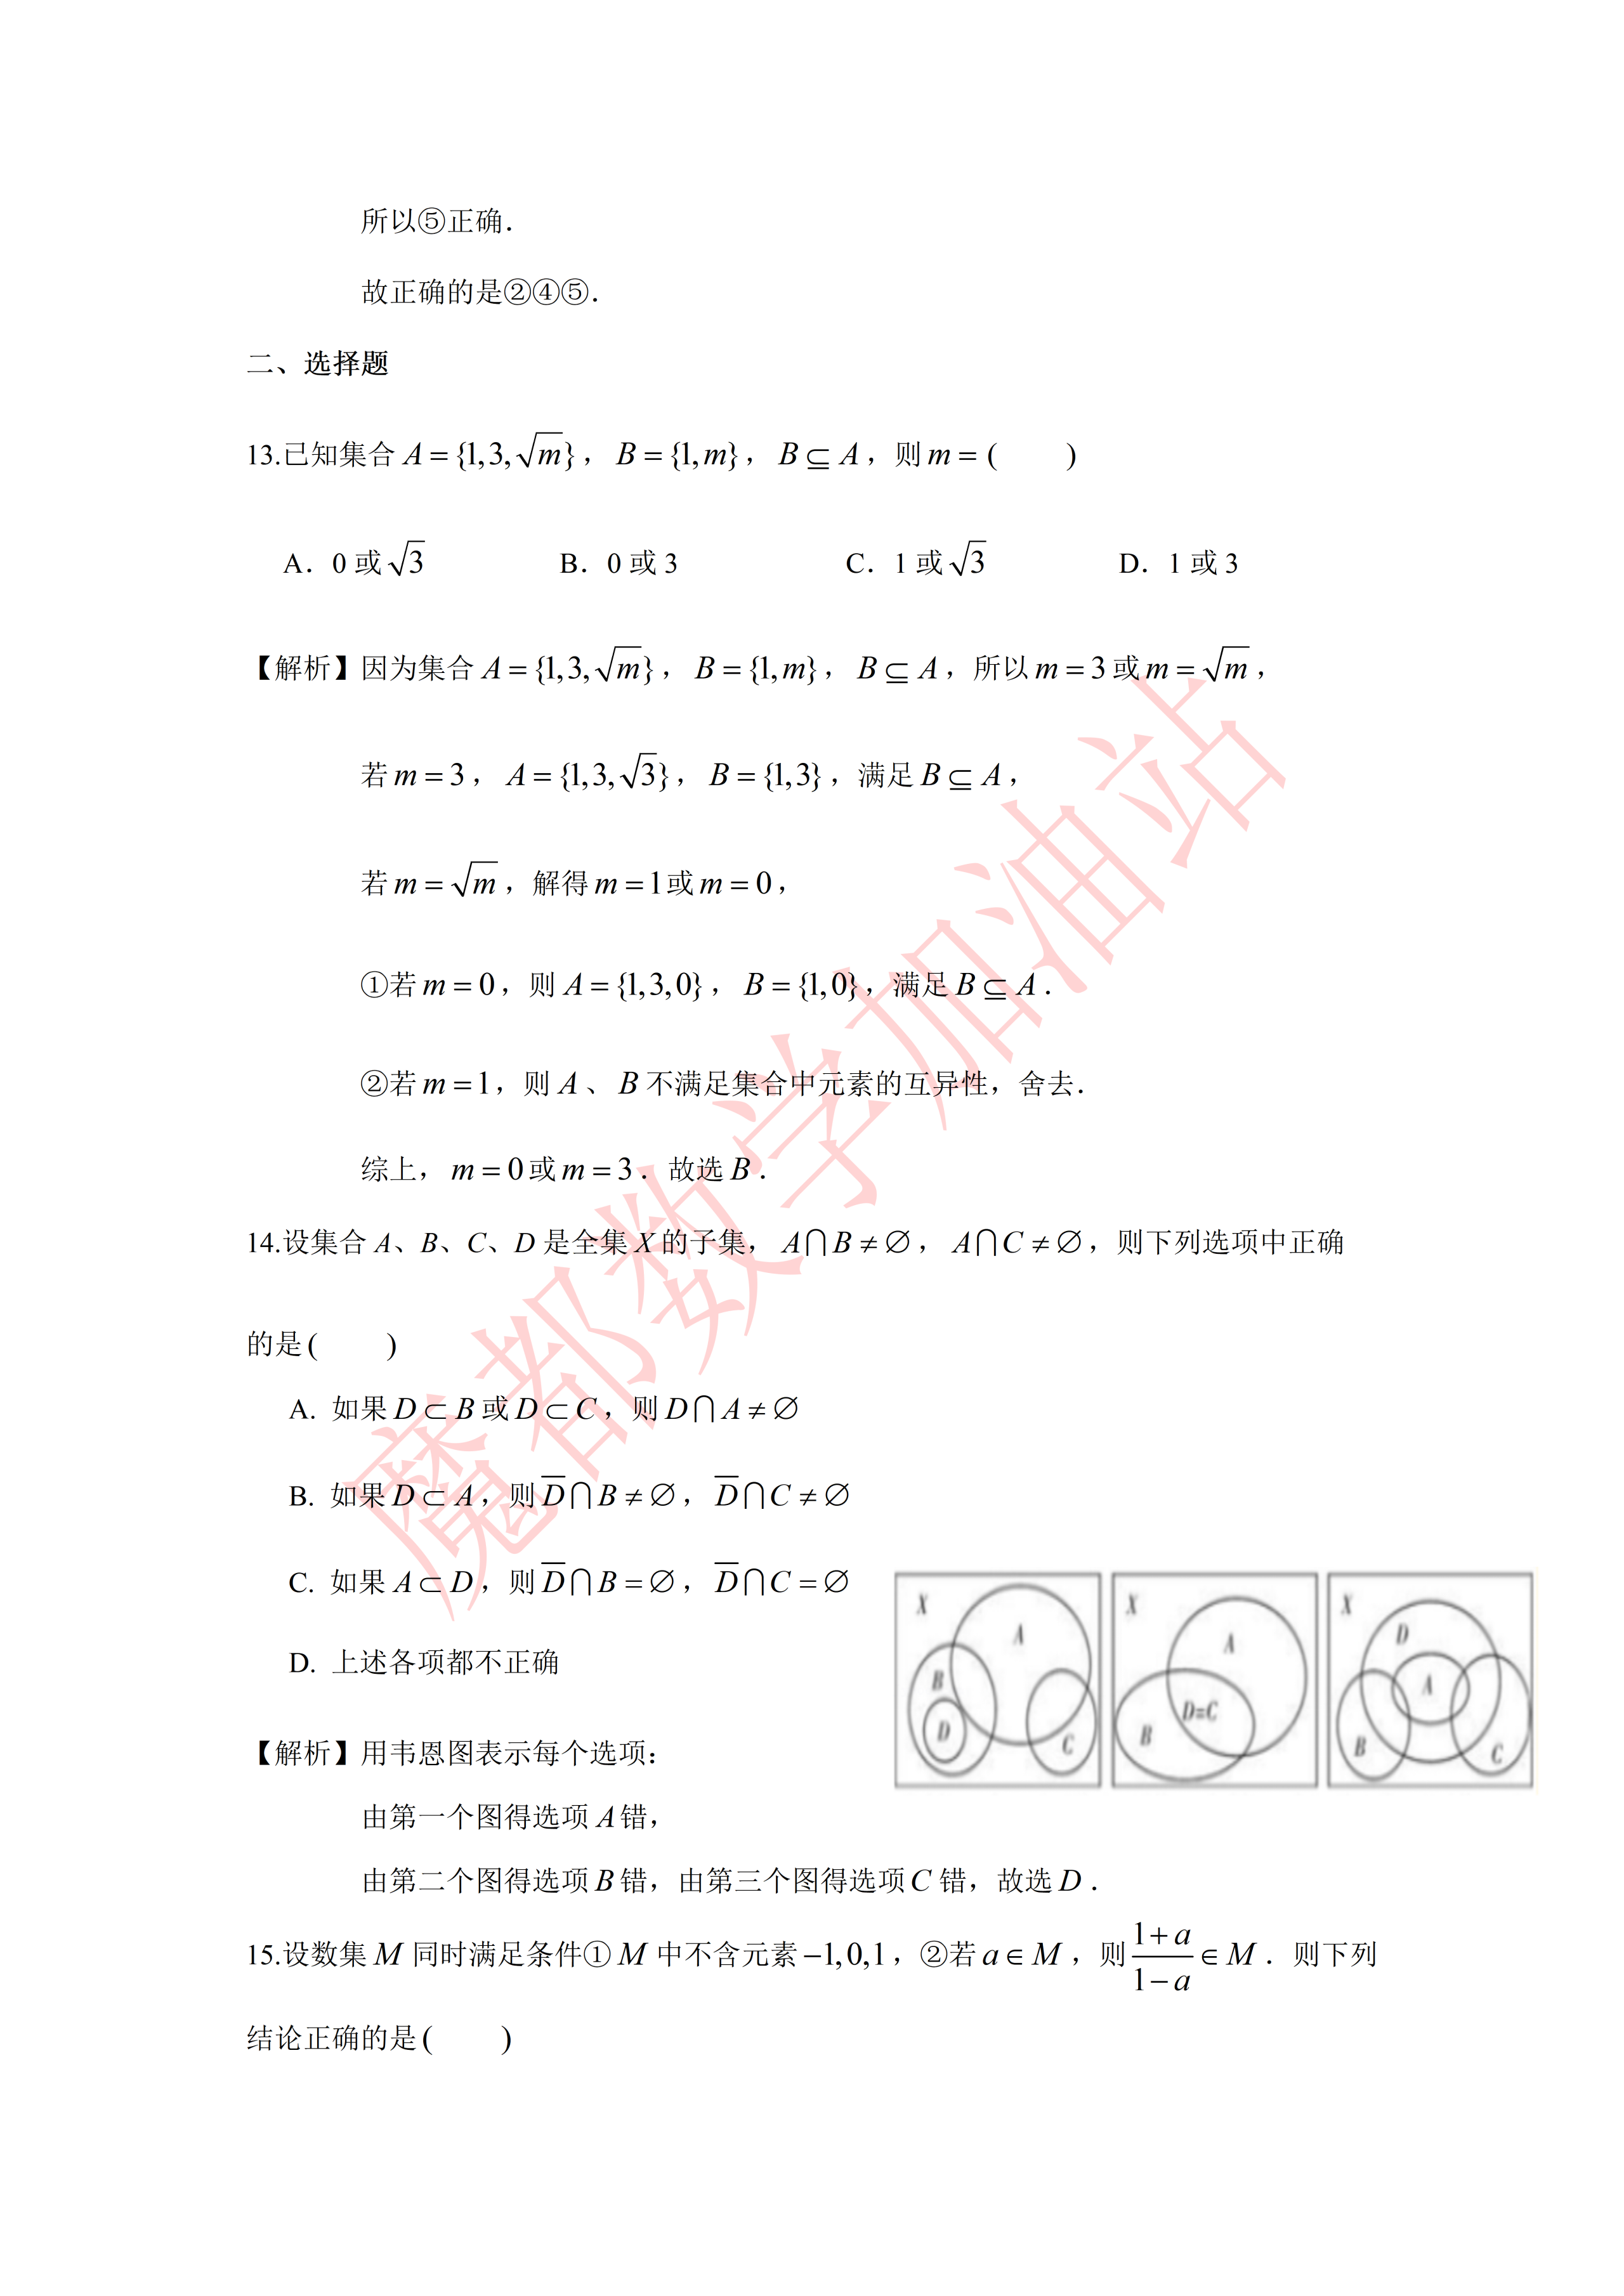
\includegraphics[width=.75\linewidth,trim=1400bp 790bp 135bp 1155bp,clip]{../原图/高一49_华师大二附中_国庆作业1/05.png}
\end{center}
\step{由第一个图得选项 $A$ 错，}
\step{由第二个图得选项 $B$ 错，由第三个图得选项 $C$ 错，故选 $D$.}
\solend
\fi

\item 设数集 $M$ 同时满足条件①$M$ 中不含元素 $-1$、$0$、$1$，②若 $a\in M$，则 $\dfrac{1+a}{1-a}\in M$．则下列结论正确的是\mbox{（\quad）}

\keepwithprev
A. 集合 $M$ 中至多有 $2$ 个元素\qquad B. 集合 $M$ 中至多有 $3$ 个元素

C. 集合 $M$ 中有且仅有 $4$ 个元素\qquad D. 集合 $M$ 中有无穷多个元素

\ifanswer
\solbegin
\step{若集合只含有一个元素，则 $\dfrac{1+a}{1-a}=a$，即 $1+a=a-a^2$，即 $-a^2=1$，不成立.}
\step{当 $a=3$ 时，$\dfrac{1+3}{1-3}=-2\in M$，所以 $\dfrac{1-2}{1+2}=-\dfrac13\in M$，所以 $\dfrac{1-\frac13}{1+\frac13}=\dfrac12\in M$，}
\step{所以 $\dfrac{1+\frac12}{1-\frac12}=3$，开始重复了，所以 $M=\left\{3,-2,-\dfrac13,\dfrac12\right\}$；}
\step{当 $a=2$ 时，$\dfrac{1+2}{1-2}=-3\in M$，所以 $\dfrac{1-3}{1+3}=-\dfrac12\in M$，所以 $\dfrac{1-\frac12}{1+\frac12}=\dfrac13\in M$，}
\step{所以 $\dfrac{1+\frac13}{1-\frac13}=2$，开始重复了，所以 $M=\left\{2,-3,-\dfrac12,-\dfrac13\right\}$，}
\step{此时也只要四个元素；}
\step{当 $a=\dfrac34\in M$，则 $7\in M$，若 $7\in M$，则 $-\dfrac43\in M$，}
\step{若 $-\dfrac43\in M$，则 $-\dfrac17\in M$，若 $-\dfrac17\in M$，有 $\dfrac34\in M$，}
\step{由归纳推理得，集合 $M$ 中有且仅有 $4$ 个元素．故选 $C$.}
\solend
\fi

\item 已知集合 $M=\{x\mid x\in\N,0<x\leqslant15\}$，$A_1$、$A_2$、$A_3$ 满足：①$A_1\cup A_2\cup A_3=M$；②每个集合都恰有 $5$ 个元素．集合 $A_i$（$i=1,2,3$）中最大元素与最小元素之和称为 $A_i$ 的特征数，记为 $X_i$（$i=1,2,3$），则 $X_1+X_2+X_3$ 的值不可能为\mbox{（\quad）}

\keepwithprev
A. $37$\qquad B. $39$\qquad C. $48$\qquad D. $57$

\ifanswer
\solbegin
\step{因为集合 $M=\{x\mid x\in\N,0<x\leqslant15\}=\{1,2,3,\cdots,15\}$，}
\step{又因为集合 $A_1$、$A_2$、$A_3$ 中，每个集合恰有 $5$ 个元素，}
\step{且 $A_1\cup A_2\cup A_3=M$ 有 $15$ 个元素，所以集合 $A_1$、$A_2$、$A_3$ 中没有重复元素，}
\step{因为 $1$ 是集合 $M$ 中数值最小的元素，$15$ 是集合 $M$ 中数值最大的元素，}
\step{所以在 $A_i$ 的特征数构成中，必有 $1$ 和 $15$，不妨设 $1\in A_1$，$15\in A_1$，}
\step{要使 $X_1+X_2+X_3$ 最大，则应该在集合 $A_1$ 中首先放置数值较小的元素，}
\step{即 $A_1=\{1,2,3,4,15\}$，所以 $5$ 与 $14$ 是剩下元素中数值最小或最大的元素，}
\step{同理，不妨设 $5\in A_2$，$14\in A_2$，接着在 $A_2$ 中再次放置数值较小的元素，}
\step{即 $A_2=\{5,6,7,8,14\}$，则 $A_3=\{9,10,11,12,13\}$，}
\step{此时 $X_1+X_2+X_3$ 有最大值为 $1+15+5+14+9+13=57$，}
\step{即 $X_1+X_2+X_3\leqslant57$；}
\step{要使 $X_1+X_2+X_3$ 最小，则在集合 $A_1$ 中首先放置数值较大的元素，}
\step{即 $A_1=\{1,12,13,14,15\}$，所以 $2$ 与 $11$ 是剩下元素中数值最小或最大的元素，}
\step{同理，不妨设 $2\in A_2$，$11\in A_2$，接着在 $A_2$ 中再次放置数值较大的元素，}
\step{即 $A_2=\{2,8,9,10,11\}$，则 $A_3=\{3,4,5,6,7\}$，}
\step{此时 $X_1+X_2+X_3$ 有最小值为 $1+15+2+11+3+7=39$，}
\step{即 $X_1+X_2+X_3\geqslant39$，}
\step{综上，$39\leqslant X_1+X_2+X_3\leqslant57$，故选 $A$.}
\solend
\fi

\end{enumerate}

\bigsec{三、解答题}

\begin{enumerate}
\setcounter{enumi}{16}

\item 已知全集为 $\R$，集合 $A=\{x\mid y=\sqrt{(2+x)(4-x)}\}$，$B=\{x\mid-1<x<m+1\}$.

\begin{enumerate}[label=(\arabic*)]
\item 若 $m=4$，求 $A\cup B$、$\overline A\cap B$；
\item 若 $B\subseteq A$，求实数 $m$ 的取值范围.
\end{enumerate}

\ifanswer
\solbegin
\stepm{(1)}{集合 $A=\{x\mid y=\sqrt{(2+x)(4-x)}\}=\{x\mid-2\leqslant x\leqslant4\}$，}
\step{当 $m=4$ 时，$B=\{x\mid-1<x<5\}$.}
\step{所以 $A\cup B=[-2,5)$，$\overline A=\{x\mid x<-2\text{ 或 }x>4\}$，$\overline A\cap B=(4,5)$.}
\stepm{(2)}{因为 $B\subseteq A$，}
% 原卷如此，照录未改（第 17 题(2)解析两处"当 C=∅／当 C≠∅"应为 B，本卷并无集合 C）
\step{当 $C=\varnothing$ 时，$m\leqslant-2$，$B\subseteq A$ 成立；}
\step{当 $C\neq\varnothing$ 时，$m>-2$，$-1<m+1\leqslant4$，解得 $-2<m\leqslant3$，}
\step{综上，$m\leqslant3$，所以实数 $m$ 的取值范围是 $(-\infty,3]$.}
\solend
\fi

\ansspace[6]

\item 用反证法证明：若 $a$、$b$、$c\in\R$，且 $x=a^2-2b+1$，$y=b^2-2c+1$，$z=c^2-2a+1$，则 $x$、$y$、$z$ 中至少有一个不小于 $0$.

\ifanswer
\solbegin
\step{假设 $x$、$y$、$z$ 均小于 $0$，即 $x=a^2-2b+1<0$①，$y=b^2-2c+1<0$②，}
\step{$z=c^2-2a+1<0$③，①$+$②$+$③得 $x+y+z=(a-1)^2+(b-1)^2+(c-1)^2<0$，}
\step{这与 $(a-1)^2+(b-1)^2+(c-1)^2\geqslant0$ 矛盾，则假设不成立，}
\step{所以 $x$、$y$、$z$ 中至少有一个不小于 $0$，得证.}
\solend
\fi

\ansspace[5]

\item 已知全集为 $\R$，实数 $a$、$b$ 满足 $a\neq b$，集合 $M=\{x\mid x^2-3x-4\leqslant0\}$，集合 $A=\{x\mid(x+a)(x+b)>0\}$，集合 $B=\{x\mid x^2+(a-2)x-2a>0\}$.

\begin{enumerate}[label=(\arabic*)]
\item 若 $\overline A=M$，求 $a$、$b$ 的值；
\item 若 $a>b>-1$，求 $A\cap B$；
\item 若 $a^2+a\in\overline B$，求 $a$ 的取值范围.
\end{enumerate}

\ifanswer
\solbegin
\stepm{(1)}{$M=\{x\mid x^2-3x-4\leqslant0\}=\{x\mid-1\leqslant x\leqslant4\}$，$A=\{x\mid(x+a)(x+b)\leqslant0\}$，}
\step{因为 $\overline A=M$，所以 $a=1$，$b=-4$ 或 $a=-4$，$b=1$.}
\stepm{(2)}{因为 $a>b>-1$，所以 $-a<-b<1$，所以 $A=\{x\mid x<-a\text{ 或 }x>-b\}$，}
\step{因为 $B=\{x\mid x^2+(a-2)x-2a>0\}=\{x\mid x<-a\text{ 或 }x>2\}$，}
\step{所以 $A\cap B=\{x\mid x<-a\text{ 或 }x>2\}$，}
\stepm{(3)}{$\overline B=\{x\mid(x-2)(x+a)\leqslant0\}$，}
% 原卷如此，照录未改（第 19 题(3)此处"a(a-1)((a-2)^2≤0"括号不配对；且由左式展开应为
% a(a-1)(a+2)^2≤0，与下句"解得 a=2 …[0,1]∪{2}"按 (a-2)^2 方自洽，见文件头清单第 2 条）
\step{由 $a^2+a\in\overline B$，得 $(a^2+a-2)(a^2+2a)\leqslant0\Leftrightarrow a(a-1)((a-2)^2\leqslant0$，}
\step{解得 $a=2$ 或 $0\leqslant a\leqslant1$，故 $a$ 的取值范围是 $[0,1]\cup\{2\}$.}
\solend
\fi

\ansspace[7]

\item 设数集 $A$ 由实数构成，若 $x\in A$（$x\neq1$ 且 $x\neq0$），则 $\dfrac{1}{1-x}\in A$.

\begin{enumerate}[label=(\arabic*)]
\item 若 $2\in A$，则 $A$ 中至少还有几个元素；
\item 集合 $A$ 是否为双元素集合？请说明理由；
\item 若 $A$ 中元素个数不超过 $8$ 个，所有元素的和为 $\dfrac{14}{3}$，且 $A$ 中有一个元素的平方等于所有元素的积，求集合 $A$.
\end{enumerate}

\ifanswer
\solbegin
\stepm{(1)}{若 $x\in A$，则 $\dfrac{1}{1-x}\in A$，又 $2\in A$，所以 $\dfrac{1}{1-2}=-1\in A$，}
\step{所以 $\dfrac{1}{1-(-1)}=\dfrac12\in A$，所以 $\dfrac{1}{1-\frac12}=2\in A$，}
% 原卷如此，照录未改（第 20 题(1)解析末句"2 个几个元素"衍一"几个"）
\step{所以 $A$ 中至少还有 $2$ 个几个元素；}
\stepm{(2)}{若 $x\in A$（$x\neq1$ 且 $x\neq0$），则 $\dfrac{1}{1-x}\in A$，}
\step{则 $\dfrac{1}{1-\frac{1}{1-x}}=\dfrac{1-x}{-x}\in A$，则 $\dfrac{1}{1-\frac{1-x}{-x}}=x\in A$}
\step{若 $A$ 为双元素集，则 $x=\dfrac{1}{1-x}$ 或 $x=\dfrac{1-x}{-x}$ 或 $\dfrac{1}{1-x}=\dfrac{1-x}{-x}$，均无解，}
\step{所以 $A$ 不可能为双元素集；}
\stepm{(3)}{由 $x\in A$，$\dfrac{1}{1-x}\in A$，得 $\dfrac{1}{1-\frac{1}{1-x}}=\dfrac{x-1}{x}\in A$，得 $\dfrac{1}{1-\frac{x-1}{x}}=x\in A$，}
\step{所以 $\left\{x,\dfrac{1}{1-x},\dfrac{x-1}{x}\right\}\subseteq A$，而 $x\cdot\dfrac{1}{1-x}\cdot\dfrac{x-1}{x}=-1$，}
\step{$A$ 中元素个数为 $3$ 的倍数，则 $A$ 中元素只有 $6$ 个，}
\step{因为 $A$ 中有一个元素的平方等于所有元素的积，}
\step{不妨设 $x^2=1$，解得 $x=-1$ 或 $x=1$（舍），则 $-1$、$\dfrac12$、$2\in A$，}
\step{所以 $-1+\dfrac12+2+m+\dfrac{1}{1-m}+\dfrac{m-1}{m}=\dfrac{14}{3}$，解得 $m=-\dfrac12$ 或 $m=3$ 或 $m=\dfrac23$，}
\step{所以 $A=\left\{\dfrac12,2,-1,-\dfrac12,3,\dfrac23\right\}$.}
\solend
\fi

\ansspace[9]

% 原卷如此，照录未改（第 21 题题干"21.求已知集合"之"求"字疑衍；"任意两个元素 a_i a_j"
% 疑脱逗号；"|a_i-a_j|≥1/30 则称"之前疑脱标点，见文件头清单第 4 条）
\item 求已知集合 $M=\left\{\dfrac{1}{k}\middle|1\leqslant k\leqslant100\text{ 且 }k\in\N^{*}\right\}$，$A=\{a_1,a_2,\cdots,a_n\}$，其中 $n\in\N^{*}$，且 $n\geqslant2$．若 $A\subseteq\N$，且对集合 $A$ 中的任意两个元素 $a_ia_j$，$i\neq j$ 都有 $|a_i-a_j|\geqslant\dfrac{1}{30}$ 则称集合 $A$ 有性质 $P$.

\begin{enumerate}[label=(\arabic*)]
\item 判断集合 $\left\{\dfrac13,\dfrac14,\dfrac15,\dfrac16,\dfrac17\right\}$ 是否具有性质 $P$；
\item 若集合 $A=\{a_1,a_2,\cdots,a_n\}$ 具有性质 $P$.

①求证：$a_i-a_j$ 的最大值大于等于 $\dfrac{n-1}{30}$；

②求 $A$ 的元素个数 $n$ 的最大值.
\end{enumerate}

\ifanswer
\solbegin
\stepm{(1)}{集合为 $\left\{\dfrac13,\dfrac14,\dfrac15,\dfrac16,\dfrac17\right\}$，又 $\dfrac16-\dfrac17=\dfrac{1}{42}<\dfrac{1}{30}$，所以该集合不具有性质 $P$；}
\stepm{(2)}{①因为集合 $A=\{a_1,a_2,\cdots,a_n\}$ 具有性质 $P$，}
\step{不妨设 $a_1<a_2<a_3<\cdots<a_n$，则 $a_i-a_j\geqslant\dfrac{1}{30}$（$i>j$），}
\step{所以 $a_n-a_1=(a_n-a_{n-1})+(a_{n-1}-a_{n-2})+\cdots+(a_2-a_1)\geqslant\dfrac{n-1}{30}$，}
\step{故 $a_i-a_j$ 的最大值大于等于 $\dfrac{n-1}{30}$；}
% 原卷如此，照录未改（第 21 题(2)②首行"a_2-a_1≥(n-1)/30"：由①同款推理只能得
% a_2-a_1≥1/30，见文件头清单第 5 条）
\step{②$A=\{a_1,a_2,\cdots,a_n\}$，不妨设 $a_1<a_2<a_3<\cdots<a_n$，}
\step{要使 $A$ 的元素个数 $n$ 最大，}
\step{则 $A$ 中的元素满足 $a_n=\dfrac{1}{k}$，$a_{n-1}=\dfrac{1}{k+1}$，$\cdots$，$a_1=\dfrac{1}{k+n-1}$（$k\in\N^{*}$），}
\step{又由①得 $a_2-a_1=\dfrac{1}{k+n-2}-\dfrac{1}{k+n-1}\geqslant\dfrac{n-1}{30}$，}
\step{所以 $(k+n-2)(k+n-1)\leqslant30$，又 $a_n-a_{n-1}=\dfrac{1}{k}-\dfrac{1}{k+1}\geqslant\dfrac{1}{30}$，}
\step{所以 $k(k+1)\leqslant30$，所以 $1\leqslant k\leqslant5$（$k\in\N^{*}$），}
\step{当 $k=5$ 时，由 $(k+n-2)(k+n-1)\leqslant30$，解得 $n\leqslant2$，$n\in\N^{*}$；}
\step{当 $k=4$ 时，由 $(k+n-2)(k+n-1)\leqslant30$，解得 $n\leqslant3$，$n\in\N^{*}$；}
\step{当 $k=3$ 时，由 $(k+n-2)(k+n-1)\leqslant30$，解得 $n\leqslant4$，$n\in\N^{*}$；}
\step{当 $k=2$ 时，由 $(k+n-2)(k+n-1)\leqslant30$，解得 $n\leqslant5$，$n\in\N^{*}$；}
\step{当 $k=1$ 时，由 $(k+n-2)(k+n-1)\leqslant30$，解得 $n\leqslant6$，$n\in\N^{*}$.}
\step{故 $A$ 的元素个数 $n$ 的最大值为 $6$，此时集合 $A=\left\{1,\dfrac12,\dfrac13,\cdots,\dfrac16\right\}$.}
\solend
\fi

\ansspace*[10]

\end{enumerate}

\end{document}
"
%
% 原始材料：微信公众号"魔都数学加油站"文章，作者破晓，连载"27学年高一49"；
% 原文标题"27学年高一49——2026-2027年上海市华师大二附中高一上国庆作业1集合与逻辑、
% 等式与不等式的性质"；页面用 JS 渲染，未见明确发布日期（页内时间戳 ≈ 2026-10-05 21:37）；
% 原文链接：https://mp.weixin.qq.com/s/XxZTOBVQslK5cZm2_BbhOg。
% 正文为 11 张 PNG 页：第 01、03、04、06、07、08、09 页 4762×6735，
% 第 02、05、10、11 页 2560×3620，均按页序读取；粉色斜排"魔都数学加油站"为卷面水印，
% 与公众号页脚一并未录入。全卷 11 页均为试卷页，无二维码/宣传页。
%
% 题号与分节：原文自第 3 题起编，填空题 3—12、选择题 13—16、解答题 17—21，共 19 题。
% 讲评版：原卷每题下直接印【答案】或【解析】——只印【答案】的 3 题（第 3、5、8 题），
% 其余 16 题均只印【解析】；解析行数已逐题按印刷行照录（一条 \step＝原卷一个印刷行）。
%
% 卷首标题：照卷面印作"2026-2027 年华师大二附中高一上国庆作业 1"（公众号标题中的"上海市"
% 卷面没有，本稿照卷面），年份区间按全稿惯例排 en dash；副标题照卷面自印的
% "集合与逻辑单元综合检测"（原卷页首标题行下方即印此行，故不另按模块口径拟名）。
% 副标题依据：全卷 19 题均为集合与常用逻辑用语内容——集合类 15 题（6—17、19—21 中除
% 反证法题外），逻辑/命题类 3 题（第 3 题否定形式、第 4 题充要条件、第 5 题反证法假设），
% 反证法证明 1 题（第 18 题）；全卷无不等式求解题，公众号标题中"等式与不等式的性质"
% 与卷面实际内容不符。
%
% 与原卷的排版差异：
%   ① 原文从第 3 题起，填空题为 3—12、选择题为 13—16、解答题为 17—21，本稿保留原题号；
%   ② 原卷每题下直接印【答案】/【解析】，本稿按全稿惯例置于答案版；只印【解析】的题
%      不另提 \ans{}（照 高一36 口径），只印【答案】的题仅给 \ans{}；
%   ③ 原卷第 8 题韦恩图排在题干右侧、第 14 题三联韦恩图排在选项（C、D）右侧，
%      本稿分别移至题干下方、解析首步之后居中排，均直接裁取原图页（02.png、05.png）；
%   ④ 数集记号原卷排作斜体/加粗 R、N、Z，本稿统一为 \R、\N、\Z、\N^*；
%      填空横线按全稿惯例排为 \blankline[4.4em]。
%
% 原卷笔误/存疑清单（均照录未改，正文中该处有 % 注）：
%   1. 第 17 题(2)解析两处"当 C=∅／当 C≠∅"应为 B（本卷并无集合 C）；
%   2. 第 19 题(3)解析"a(a-1)((a-2)^2≤0"括号不配对（多一枚左括号）；且由
%      (a^2+a-2)(a^2+2a)≤0 展开应为 a(a-1)(a+2)^2≤0，与原卷结论"解得 a=2 …
%      [0,1]∪{2}"恰按 (a-2)^2 自洽——因式分解与原式不符，结论按 (a-2)^2 自洽，均照录；
%   3. 第 20 题(1)解析末句"至少还有 2 个几个元素"衍一"几个"；
%   4. 第 21 题题干"21.求已知集合"之"求"字疑衍；"任意两个元素 a_i a_j"疑脱逗号；
%      "≥1/30 则称"之前疑脱标点；
%   5. 第 21 题(2)②解析"a_2-a_1≥(n-1)/30"：由①同款推理只能得 a_2-a_1≥1/30，
%      原卷如此，照录未改（后续 (k+n-2)(k+n-1)≤30 即按该行推得）。
%
\documentclass[a4paper,11pt]{article}
\usepackage{common}

\begin{document}

\examtitlest[3]{2026--2027 年华师大二附中高一上国庆作业 1}{集合与逻辑单元综合检测}

\bigsec{一、填空题}

\begin{enumerate}
\setcounter{enumi}{2}

\item “若 $x^2-x-2\leqslant0$，则 $-1\leqslant x\leqslant2$”的否定形式为\blankline[4.4em].

\ifanswer
\ans{若 $x^2-x-2>0$，则 $x<-1$ 或 $x>2$}
\fi

\item 已知 $p:|x-3|<5$，$q:1-a<x<2a-3$，且 $p$ 是 $q$ 的充分非必要条件，则实数 $a$ 的取值范围是\blankline[4.4em].

\ifanswer
\solbegin
\step{由 $|x-3|<5$ 得 $-2<x<8$，}
\step{又 $p$ 是 $q$ 的充分不必要条件，所以 $(-2,8)\subset(1-a,2a-3)$，}
\step{即 $\begin{cases}-2\geqslant1-a\\ 8\leqslant2a-3\\ (2a-3)-(1-a)\neq8-(-2)\end{cases}$，解得 $a\geqslant\dfrac{11}{2}$，实数 $a$ 的取值范围是 $\left[\dfrac{11}{2},+\infty\right)$.}
\solend
\fi

\item 用反证法证明命题“设 $a$、$b\in\R$，则方程 $a_1x^2+b_1x+c_1=0$ 与 $a_2x^2+b_2x+c_2=0$ 至少有一个实根”时要做的假设是\blankline[4.4em].

\ifanswer
\ans{假设 $a$、$b\in\R$，方程 $a_1x^2+b_1x+c_1=0$ 与 $a_2x^2+b_2x+c_2=0$ 都没有实根}
\fi

\item 设集合 $A=\{x\mid x^2-mx+6=0,x\in\R\}$，且 $A\cap\{2,3\}=A$，则实数 $m$ 的取值范围是\blankline[4.4em].

\ifanswer
\solbegin
\step{由 $A\cap\{2,3\}=A$，得 $A\subseteq\{2,3\}$，}
\step{当 $A=\varnothing$ 时，$\Delta=m^2-24<0$，解得 $-2\sqrt6<m<2\sqrt6$；}
\step{当 $A=\{2\}$ 时，$\begin{cases}2^2-2m+6=0\\ \Delta=m^2-24=0\end{cases}$，无解；}
\step{当 $A=\{3\}$ 时，$\begin{cases}3^2-3m+6=0\\ \Delta=m^2-24=0\end{cases}$，无解；}
\step{当 $A=\{2,3\}$ 时，$\begin{cases}3^2-3m+6=0\\ 2^2-2m+6=0\end{cases}$，解得 $m=5$，}
\step{所以实数 $m$ 的取值范围是 $(-2\sqrt6,2\sqrt6)\cup\{5\}$.}
\solend
\fi

\item 已知 $a\in\R$，集合 $A=\left\{x\middle|\dfrac12a-1<x<\dfrac12a+1\right\}$，设关于 $x$ 的不等式 $ax<a^2+x-1$ 的解集为 $B$，若 $A\subset B$，则实数 $a$ 的取值范围为\blankline[4.4em].

\ifanswer
\solbegin
\step{因为 $ax<a^2+x-1$，所以 $(a-1)x<(a-1)(a+1)$，}
\step{①当 $a=1$ 时，$B=\varnothing$，$A\subset B$ 不可能成立；}
\step{②当 $a<1$ 时，$B=\{x\mid x>a+1\}$，因为 $A\subset B$，所以 $\dfrac12a-1\geqslant a+1$，}
\step{即 $a\leqslant-4$；}
\step{③当 $a>1$ 时，$B=\{x\mid x<a+1\}$，因为 $A\subset B$，所以 $\dfrac12a+1\leqslant a+1$，}
\step{即 $a>1$；}
\step{综上所述，实数 $a$ 的取值范围为 $(-\infty,-4]\cup(1,+\infty)$.}
\solend
\fi

\needvspace{8\baselineskip}

\item 已知 $U$ 为全集，$M$、$P$、$S$ 是 $U$ 的三个子集，用交、并、补关系将图中的阴影部分表示出来\blankline[4.4em].

\begin{center}
% 原图第 2 页题旁韦恩图直接裁取（原卷排于题干右侧）。
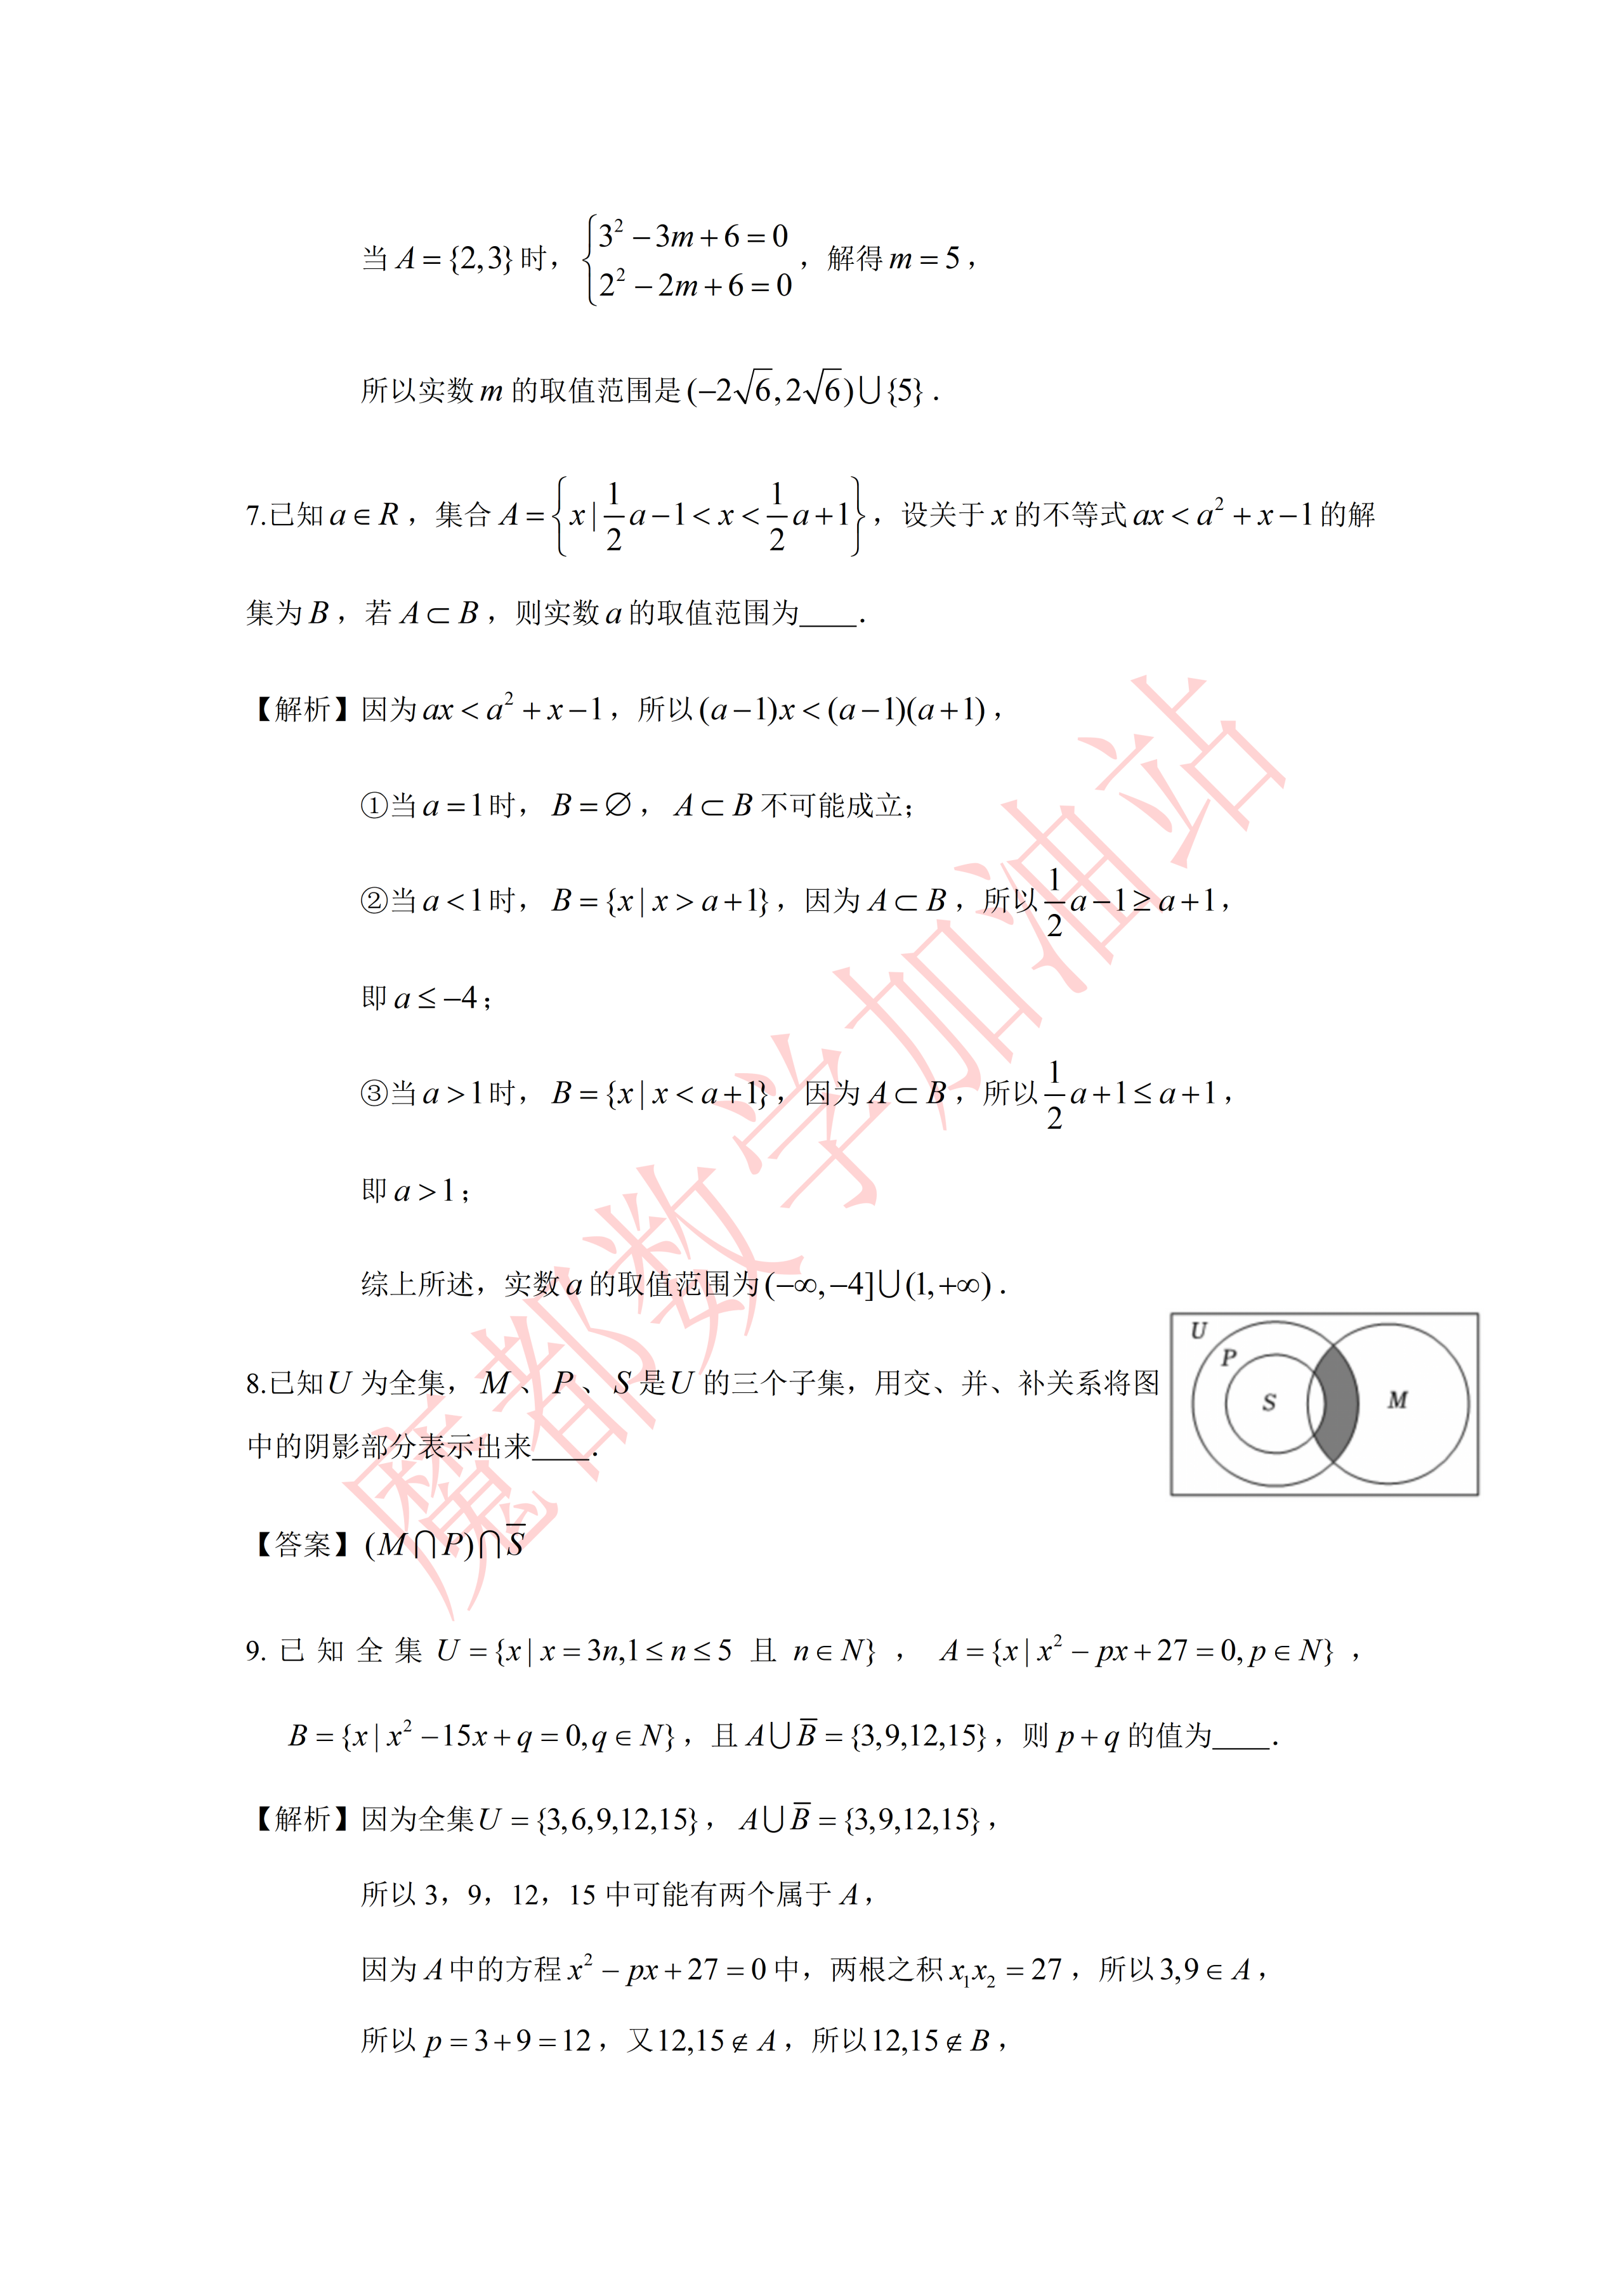
\includegraphics[width=.38\linewidth,trim=1835bp 1255bp 220bp 1565bp,clip]{../原图/高一49_华师大二附中_国庆作业1/02.png}
\end{center}

\ifanswer
\ans{$(M\cap P)\cap\overline S$}
\fi

\item 已知全集 $U=\{x\mid x=3n,1\leqslant n\leqslant5\text{ 且 }n\in\N\}$，$A=\{x\mid x^2-px+27=0,p\in\N\}$，$B=\{x\mid x^2-15x+q=0,q\in\N\}$，且 $A\cup\overline B=\{3,9,12,15\}$，则 $p+q$ 的值为\blankline[4.4em].

\ifanswer
\solbegin
\step{因为全集 $U=\{3,6,9,12,15\}$，$A\cup\overline B=\{3,9,12,15\}$，}
\step{所以 $3$、$9$、$12$、$15$ 中可能有两个属于 $A$，}
\step{因为 $A$ 中的方程 $x^2-px+27=0$ 中，两根之积 $x_1x_2=27$，所以 $3,9\in A$，}
\step{所以 $p=3+9=12$，又 $12,15\notin A$，所以 $12,15\notin B$，}
\step{因为 $B$ 中的方程 $x^2-15x+q=0$ 中，两根之和 $x_3+x_4=15$，所以 $6,9\in B$，}
\step{则 $q=6\times9=54$，所以 $p+q=66$.}
\solend
\fi

\item 已知集合 $A=\{x\mid x^2+(2a-3)x-3a=0,a\in\R,x\in\R\}$，集合 $B=\{x\mid x^2+(a-3)x+a^2-3a=0,a\in\R,x\in\R\}$，若 $A\neq B$，$A\cap B\neq\varnothing$，则 $A\cup B=$\blankline[4.4em].

\ifanswer
\solbegin
\step{设两个集合中的方程的公共解是 $b$，}
\step{由 $b^2+(2a-3)b-3a=b^2+(a-3)b+a^2-3a$，得 $ab=a^2$，}
\step{则 $a=0$ 或 $b=a$，}
\step{当 $a=0$ 时，不合题意，}
\step{当 $b=a$ 时，即两个方程的公共解为 $b=a$，}
\step{将 $b=a$ 代入方程，得 $a^2=2a$，$a=2$，}
\step{所以 $A=\{2,-3\}$，$B=\{-1,2\}$，所以 $A\cup B=\{-1,2,-3\}$.}
\solend
\fi

\item 已知一个有四个数字元素的集合 $S$，$S$ 的所有子集的元素和（空集的元素和认为是 $0$）的总和为 $16192$，则 $S$ 的元素之和等于\blankline[4.4em].

\ifanswer
\solbegin
\step{设 $S=\{a_1,a_2,a_3,a_4\}$，$S$ 的每个元素在所有子集中均出现 $2^3$ 次，}
\step{故 $(a_1+a_2+a_3+a_4)\cdot2^3=16192$，所以 $a_1+a_2+a_3+a_4=2024$，}
\step{故 $S$ 的元素之和等于 $2024$.}
\solend
\fi

\item 设 $P$ 为非空实数集满足：对任意给定的 $x,y\in P$（$x$、$y$ 可以相同），都有 $x+y\in P,x-y\in P,xy\in P$，则称 $P$ 为封闭集．关于封闭集有下列结论：

①集合 $P=\{-2,-1,0,1,2\}$ 为封闭集；

②集合 $P=\{x\mid x=2n,n\in\Z\}$ 为封闭集；

③若集合 $P_1$、$P_2$ 为封闭集，则 $P_1\cup P_2$ 为封闭集；

④若集合 $P$ 为封闭集，则一定有 $0\in P$；

⑤若集合 $P_1$、$P_2$ 为封闭集，则 $P_1\cap P_2$ 为封闭集.

其中正确结论的序号是\blankline[4.4em].

\ifanswer
\solbegin
\step{对于集合 $P=\{-2,-1,0,1,2\}$，取 $x=2$，$y=-2$，则 $x-y=2-(-2)=4\notin P$，}
\step{不满足封闭集的定义，所以①错误.}
\step{对于集合 $P=\{x\mid x=2n,n\in\Z\}$，设 $x=2n_1$，$y=2n_2$，$n_1,n_2\in\Z$.}
\step{$x+y=2n_1+2n_2=2(n_1+n_2)$，因为 $n_1+n_2\in\Z$，所以 $x+y\in P$.}
\step{$x-y=2n_1-2n_2=2(n_1-n_2)$，因为 $n_1-n_2\in\Z$，所以 $x-y\in P$.}
\step{$xy=2n_1\times2n_2=4n_1n_2=2(2n_1n_2)$，因为 $2n_1n_2\in\Z$，所以 $xy\in P$.}
\step{满足封闭集的定义，所以②正确.}
\step{令 $P_1=\{x\mid x=2n,n\in\Z\}$，$P_2=\{x\mid x=3n,n\in\Z\}$，都是封闭集.}
\step{$P_1\cup P_2$ 中，取 $x=2(x\in P_1)$，$y=3(y\in P_2)$，$x+y=5\notin P_1\cup P_2$，}
\step{不满足封闭集的定义，所以③错误.}
\step{因为对任意 $x\in P$，有 $x-x=0\in P$，}
\step{所以若集合 $P$ 为封闭集，则一定有 $0\in P$，所以④正确.}
\step{因为 $P_1$、$P_2$ 为封闭集，设 $x,y\in P_1\cap P_2$，则 $x,y\in P_1$ 且 $x,y\in P_2$.}
\step{因为 $P_1$ 是封闭集，所以 $x+y\in P_1,x-y\in P_1,xy\in P_1$.}
\step{因为 $P_2$ 是封闭集，所以 $x+y\in P_2,x-y\in P_2,xy\in P_2$.}
\step{所以 $x+y\in P_1\cap P_2,x-y\in P_1\cap P_2,xy\in P_1\cap P_2$，满足封闭集的定义，}
\step{所以⑤正确.}
\step{故正确的是②④⑤.}
\solend
\fi

\end{enumerate}

\bigsec{二、选择题}

\begin{enumerate}
\setcounter{enumi}{12}

\item 已知集合 $A=\{1,3,\sqrt m\}$，$B=\{1,m\}$，$B\subseteq A$，则 $m=$\mbox{（\quad）}

\keepwithprev
A. $0$ 或 $\sqrt3$\qquad B. $0$ 或 $3$

C. $1$ 或 $\sqrt3$\qquad D. $1$ 或 $3$

\ifanswer
\solbegin
\step{因为集合 $A=\{1,3,\sqrt m\}$，$B=\{1,m\}$，$B\subseteq A$，所以 $m=3$ 或 $m=\sqrt m$，}
\step{若 $m=3$，$A=\{1,3,\sqrt3\}$，$B=\{1,3\}$，满足 $B\subseteq A$，}
\step{若 $m=\sqrt m$，解得 $m=1$ 或 $m=0$，}
\step{①若 $m=0$，则 $A=\{1,3,0\}$，$B=\{1,0\}$，满足 $B\subseteq A$.}
\step{②若 $m=1$，则 $A$、$B$ 不满足集合中元素的互异性，舍去.}
\step{综上，$m=0$ 或 $m=3$．故选 $B$.}
\solend
\fi

\needvspace{10\baselineskip}

\item 设集合 $A$、$B$、$C$、$D$ 是全集 $X$ 的子集，$A\cap B\neq\varnothing$，$A\cap C\neq\varnothing$，则下列选项中正确的是\mbox{（\quad）}

\keepwithprev
A. 如果 $D\subset B$ 或 $D\subset C$，则 $D\cap A\neq\varnothing$

B. 如果 $D\subset A$，则 $\overline D\cap B\neq\varnothing$，$\overline D\cap C\neq\varnothing$

C. 如果 $A\subset D$，则 $\overline D\cap B=\varnothing$，$\overline D\cap C=\varnothing$

D. 上述各项都不正确

\ifanswer
\solbegin
\step{用韦恩图表示每个选项：}
\begin{center}
% 原图第 5 页解析配图（三联韦恩图）直接裁取（原卷排于选项 C、D 右侧）。
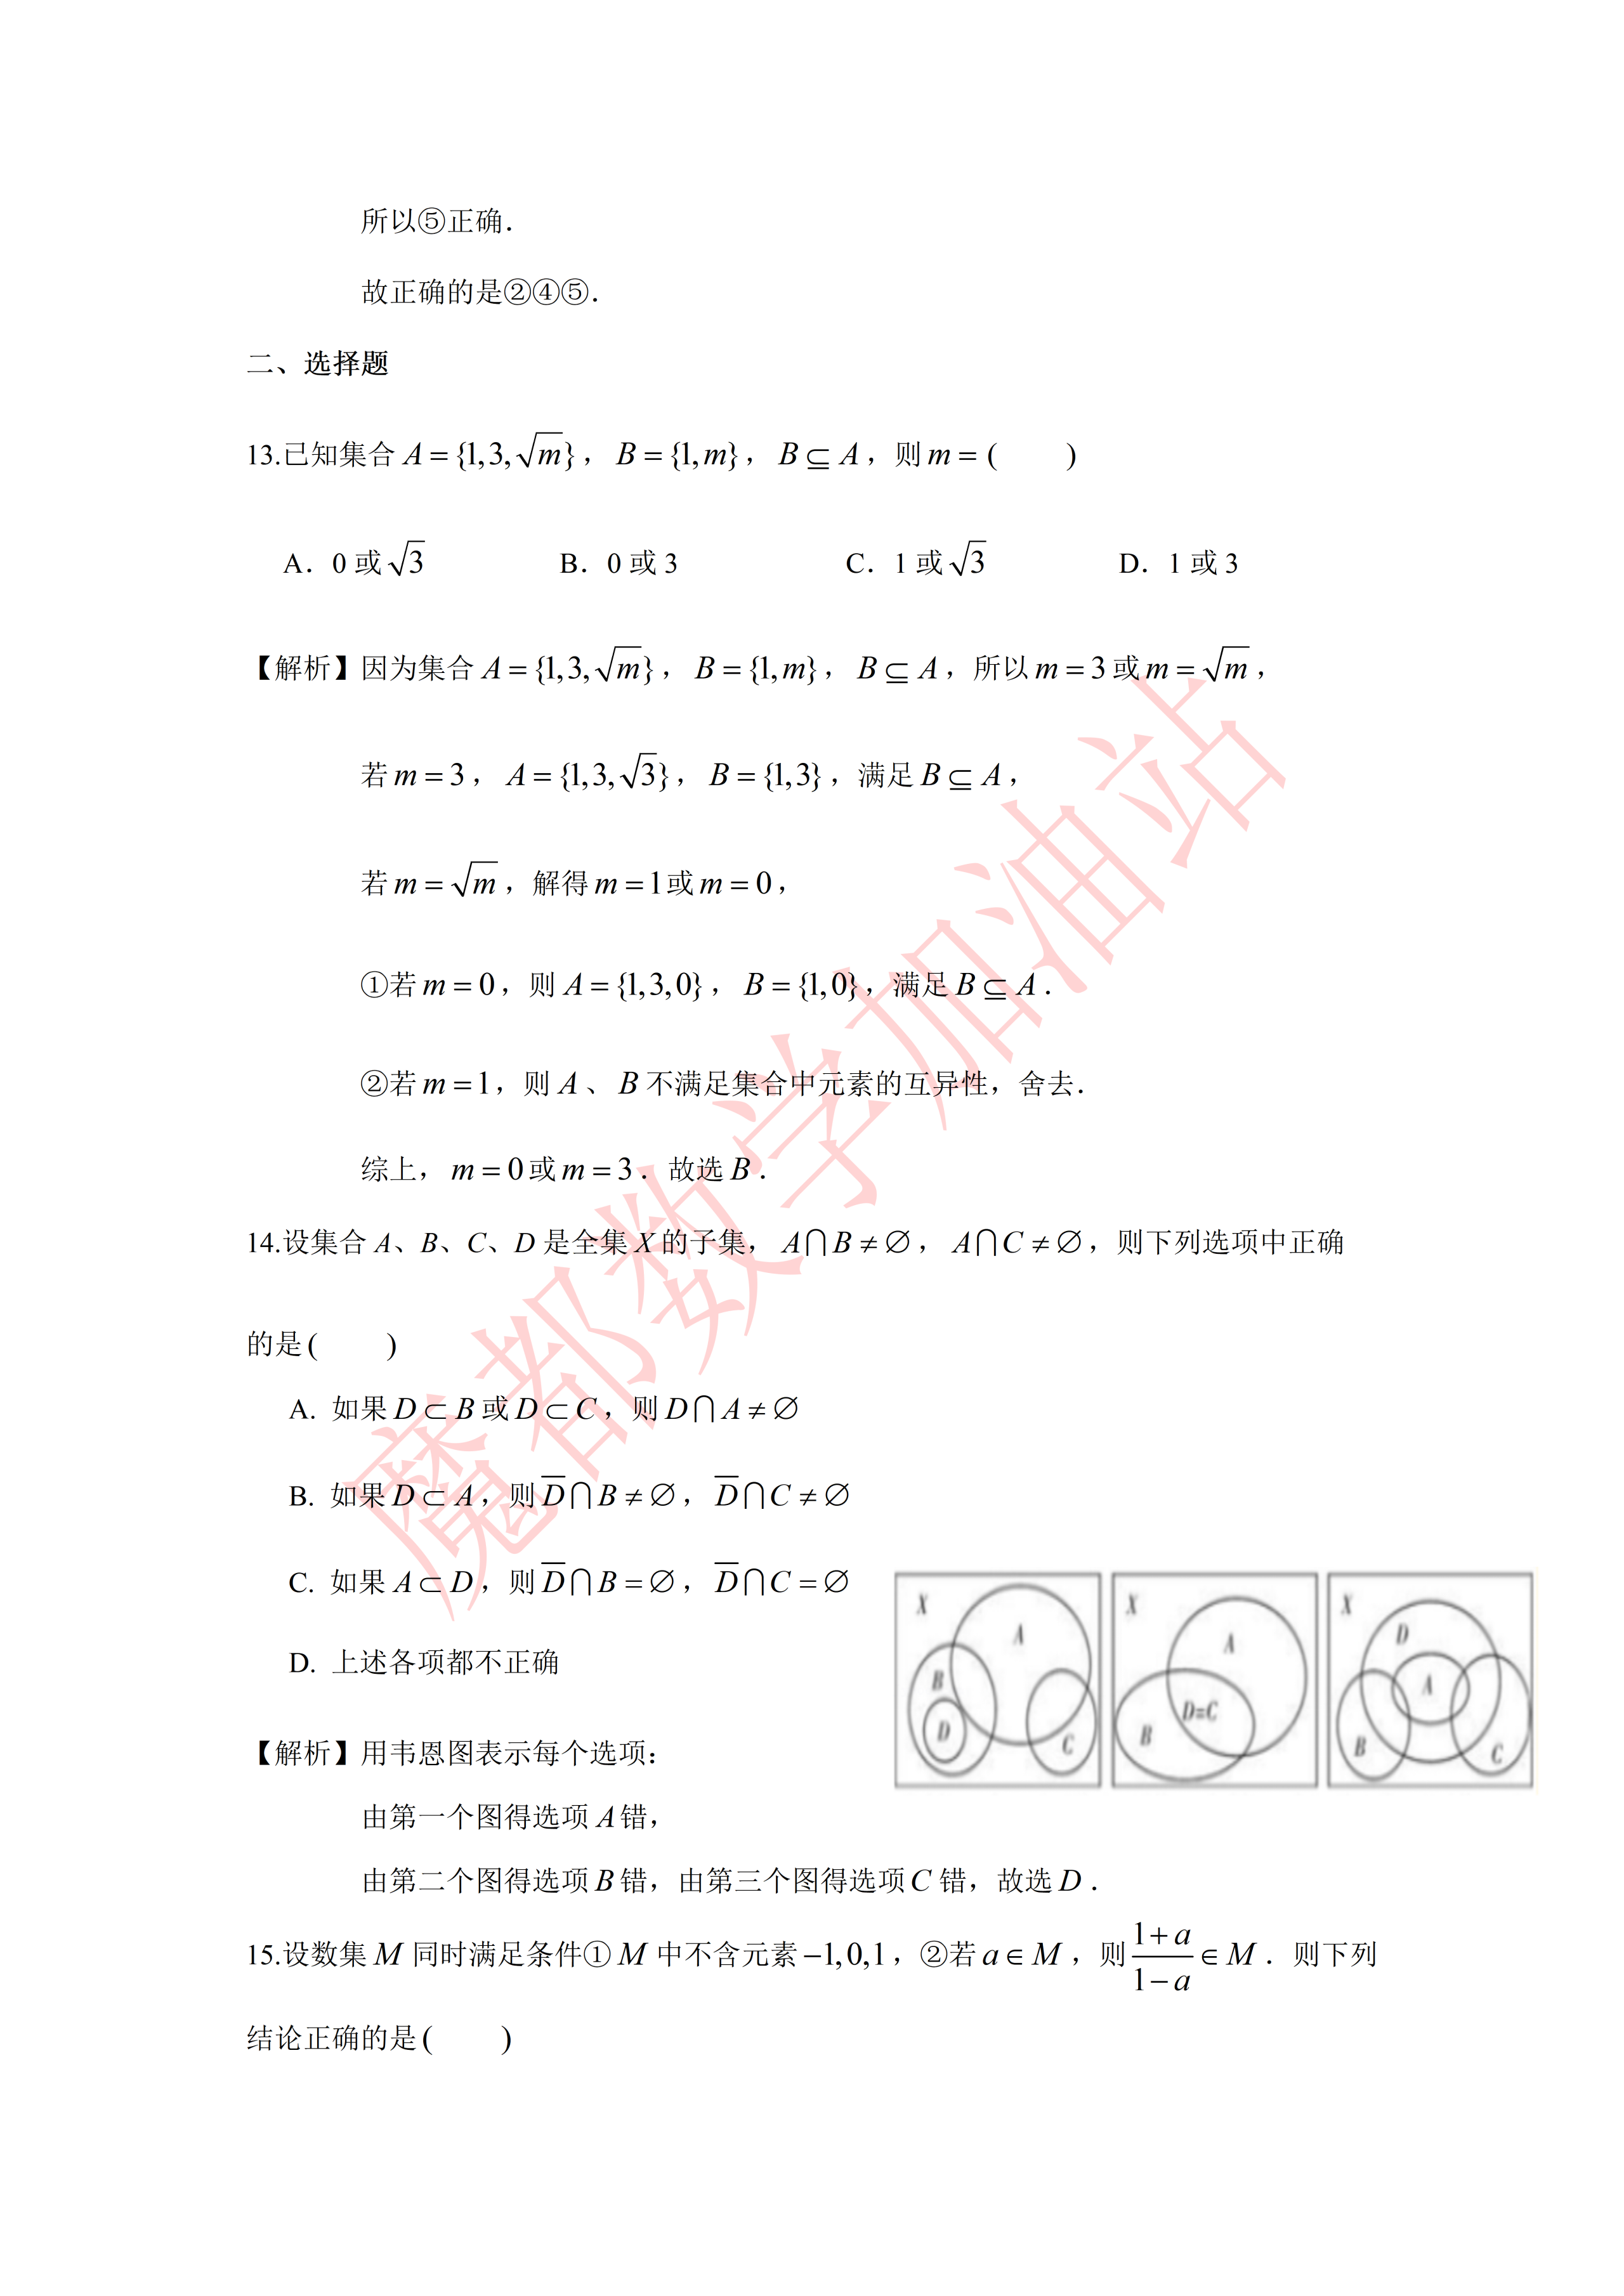
\includegraphics[width=.75\linewidth,trim=1400bp 790bp 135bp 1155bp,clip]{../原图/高一49_华师大二附中_国庆作业1/05.png}
\end{center}
\step{由第一个图得选项 $A$ 错，}
\step{由第二个图得选项 $B$ 错，由第三个图得选项 $C$ 错，故选 $D$.}
\solend
\fi

\item 设数集 $M$ 同时满足条件①$M$ 中不含元素 $-1$、$0$、$1$，②若 $a\in M$，则 $\dfrac{1+a}{1-a}\in M$．则下列结论正确的是\mbox{（\quad）}

\keepwithprev
A. 集合 $M$ 中至多有 $2$ 个元素\qquad B. 集合 $M$ 中至多有 $3$ 个元素

C. 集合 $M$ 中有且仅有 $4$ 个元素\qquad D. 集合 $M$ 中有无穷多个元素

\ifanswer
\solbegin
\step{若集合只含有一个元素，则 $\dfrac{1+a}{1-a}=a$，即 $1+a=a-a^2$，即 $-a^2=1$，不成立.}
\step{当 $a=3$ 时，$\dfrac{1+3}{1-3}=-2\in M$，所以 $\dfrac{1-2}{1+2}=-\dfrac13\in M$，所以 $\dfrac{1-\frac13}{1+\frac13}=\dfrac12\in M$，}
\step{所以 $\dfrac{1+\frac12}{1-\frac12}=3$，开始重复了，所以 $M=\left\{3,-2,-\dfrac13,\dfrac12\right\}$；}
\step{当 $a=2$ 时，$\dfrac{1+2}{1-2}=-3\in M$，所以 $\dfrac{1-3}{1+3}=-\dfrac12\in M$，所以 $\dfrac{1-\frac12}{1+\frac12}=\dfrac13\in M$，}
\step{所以 $\dfrac{1+\frac13}{1-\frac13}=2$，开始重复了，所以 $M=\left\{2,-3,-\dfrac12,-\dfrac13\right\}$，}
\step{此时也只要四个元素；}
\step{当 $a=\dfrac34\in M$，则 $7\in M$，若 $7\in M$，则 $-\dfrac43\in M$，}
\step{若 $-\dfrac43\in M$，则 $-\dfrac17\in M$，若 $-\dfrac17\in M$，有 $\dfrac34\in M$，}
\step{由归纳推理得，集合 $M$ 中有且仅有 $4$ 个元素．故选 $C$.}
\solend
\fi

\item 已知集合 $M=\{x\mid x\in\N,0<x\leqslant15\}$，$A_1$、$A_2$、$A_3$ 满足：①$A_1\cup A_2\cup A_3=M$；②每个集合都恰有 $5$ 个元素．集合 $A_i$（$i=1,2,3$）中最大元素与最小元素之和称为 $A_i$ 的特征数，记为 $X_i$（$i=1,2,3$），则 $X_1+X_2+X_3$ 的值不可能为\mbox{（\quad）}

\keepwithprev
A. $37$\qquad B. $39$\qquad C. $48$\qquad D. $57$

\ifanswer
\solbegin
\step{因为集合 $M=\{x\mid x\in\N,0<x\leqslant15\}=\{1,2,3,\cdots,15\}$，}
\step{又因为集合 $A_1$、$A_2$、$A_3$ 中，每个集合恰有 $5$ 个元素，}
\step{且 $A_1\cup A_2\cup A_3=M$ 有 $15$ 个元素，所以集合 $A_1$、$A_2$、$A_3$ 中没有重复元素，}
\step{因为 $1$ 是集合 $M$ 中数值最小的元素，$15$ 是集合 $M$ 中数值最大的元素，}
\step{所以在 $A_i$ 的特征数构成中，必有 $1$ 和 $15$，不妨设 $1\in A_1$，$15\in A_1$，}
\step{要使 $X_1+X_2+X_3$ 最大，则应该在集合 $A_1$ 中首先放置数值较小的元素，}
\step{即 $A_1=\{1,2,3,4,15\}$，所以 $5$ 与 $14$ 是剩下元素中数值最小或最大的元素，}
\step{同理，不妨设 $5\in A_2$，$14\in A_2$，接着在 $A_2$ 中再次放置数值较小的元素，}
\step{即 $A_2=\{5,6,7,8,14\}$，则 $A_3=\{9,10,11,12,13\}$，}
\step{此时 $X_1+X_2+X_3$ 有最大值为 $1+15+5+14+9+13=57$，}
\step{即 $X_1+X_2+X_3\leqslant57$；}
\step{要使 $X_1+X_2+X_3$ 最小，则在集合 $A_1$ 中首先放置数值较大的元素，}
\step{即 $A_1=\{1,12,13,14,15\}$，所以 $2$ 与 $11$ 是剩下元素中数值最小或最大的元素，}
\step{同理，不妨设 $2\in A_2$，$11\in A_2$，接着在 $A_2$ 中再次放置数值较大的元素，}
\step{即 $A_2=\{2,8,9,10,11\}$，则 $A_3=\{3,4,5,6,7\}$，}
\step{此时 $X_1+X_2+X_3$ 有最小值为 $1+15+2+11+3+7=39$，}
\step{即 $X_1+X_2+X_3\geqslant39$，}
\step{综上，$39\leqslant X_1+X_2+X_3\leqslant57$，故选 $A$.}
\solend
\fi

\end{enumerate}

\bigsec{三、解答题}

\begin{enumerate}
\setcounter{enumi}{16}

\item 已知全集为 $\R$，集合 $A=\{x\mid y=\sqrt{(2+x)(4-x)}\}$，$B=\{x\mid-1<x<m+1\}$.

\begin{enumerate}[label=(\arabic*)]
\item 若 $m=4$，求 $A\cup B$、$\overline A\cap B$；
\item 若 $B\subseteq A$，求实数 $m$ 的取值范围.
\end{enumerate}

\ifanswer
\solbegin
\stepm{(1)}{集合 $A=\{x\mid y=\sqrt{(2+x)(4-x)}\}=\{x\mid-2\leqslant x\leqslant4\}$，}
\step{当 $m=4$ 时，$B=\{x\mid-1<x<5\}$.}
\step{所以 $A\cup B=[-2,5)$，$\overline A=\{x\mid x<-2\text{ 或 }x>4\}$，$\overline A\cap B=(4,5)$.}
\stepm{(2)}{因为 $B\subseteq A$，}
% 原卷如此，照录未改（第 17 题(2)解析两处"当 C=∅／当 C≠∅"应为 B，本卷并无集合 C）
\step{当 $C=\varnothing$ 时，$m\leqslant-2$，$B\subseteq A$ 成立；}
\step{当 $C\neq\varnothing$ 时，$m>-2$，$-1<m+1\leqslant4$，解得 $-2<m\leqslant3$，}
\step{综上，$m\leqslant3$，所以实数 $m$ 的取值范围是 $(-\infty,3]$.}
\solend
\fi

\ansspace[6]

\item 用反证法证明：若 $a$、$b$、$c\in\R$，且 $x=a^2-2b+1$，$y=b^2-2c+1$，$z=c^2-2a+1$，则 $x$、$y$、$z$ 中至少有一个不小于 $0$.

\ifanswer
\solbegin
\step{假设 $x$、$y$、$z$ 均小于 $0$，即 $x=a^2-2b+1<0$①，$y=b^2-2c+1<0$②，}
\step{$z=c^2-2a+1<0$③，①$+$②$+$③得 $x+y+z=(a-1)^2+(b-1)^2+(c-1)^2<0$，}
\step{这与 $(a-1)^2+(b-1)^2+(c-1)^2\geqslant0$ 矛盾，则假设不成立，}
\step{所以 $x$、$y$、$z$ 中至少有一个不小于 $0$，得证.}
\solend
\fi

\ansspace[5]

\item 已知全集为 $\R$，实数 $a$、$b$ 满足 $a\neq b$，集合 $M=\{x\mid x^2-3x-4\leqslant0\}$，集合 $A=\{x\mid(x+a)(x+b)>0\}$，集合 $B=\{x\mid x^2+(a-2)x-2a>0\}$.

\begin{enumerate}[label=(\arabic*)]
\item 若 $\overline A=M$，求 $a$、$b$ 的值；
\item 若 $a>b>-1$，求 $A\cap B$；
\item 若 $a^2+a\in\overline B$，求 $a$ 的取值范围.
\end{enumerate}

\ifanswer
\solbegin
\stepm{(1)}{$M=\{x\mid x^2-3x-4\leqslant0\}=\{x\mid-1\leqslant x\leqslant4\}$，$A=\{x\mid(x+a)(x+b)\leqslant0\}$，}
\step{因为 $\overline A=M$，所以 $a=1$，$b=-4$ 或 $a=-4$，$b=1$.}
\stepm{(2)}{因为 $a>b>-1$，所以 $-a<-b<1$，所以 $A=\{x\mid x<-a\text{ 或 }x>-b\}$，}
\step{因为 $B=\{x\mid x^2+(a-2)x-2a>0\}=\{x\mid x<-a\text{ 或 }x>2\}$，}
\step{所以 $A\cap B=\{x\mid x<-a\text{ 或 }x>2\}$，}
\stepm{(3)}{$\overline B=\{x\mid(x-2)(x+a)\leqslant0\}$，}
% 原卷如此，照录未改（第 19 题(3)此处"a(a-1)((a-2)^2≤0"括号不配对；且由左式展开应为
% a(a-1)(a+2)^2≤0，与下句"解得 a=2 …[0,1]∪{2}"按 (a-2)^2 方自洽，见文件头清单第 2 条）
\step{由 $a^2+a\in\overline B$，得 $(a^2+a-2)(a^2+2a)\leqslant0\Leftrightarrow a(a-1)((a-2)^2\leqslant0$，}
\step{解得 $a=2$ 或 $0\leqslant a\leqslant1$，故 $a$ 的取值范围是 $[0,1]\cup\{2\}$.}
\solend
\fi

\ansspace[7]

\item 设数集 $A$ 由实数构成，若 $x\in A$（$x\neq1$ 且 $x\neq0$），则 $\dfrac{1}{1-x}\in A$.

\begin{enumerate}[label=(\arabic*)]
\item 若 $2\in A$，则 $A$ 中至少还有几个元素；
\item 集合 $A$ 是否为双元素集合？请说明理由；
\item 若 $A$ 中元素个数不超过 $8$ 个，所有元素的和为 $\dfrac{14}{3}$，且 $A$ 中有一个元素的平方等于所有元素的积，求集合 $A$.
\end{enumerate}

\ifanswer
\solbegin
\stepm{(1)}{若 $x\in A$，则 $\dfrac{1}{1-x}\in A$，又 $2\in A$，所以 $\dfrac{1}{1-2}=-1\in A$，}
\step{所以 $\dfrac{1}{1-(-1)}=\dfrac12\in A$，所以 $\dfrac{1}{1-\frac12}=2\in A$，}
% 原卷如此，照录未改（第 20 题(1)解析末句"2 个几个元素"衍一"几个"）
\step{所以 $A$ 中至少还有 $2$ 个几个元素；}
\stepm{(2)}{若 $x\in A$（$x\neq1$ 且 $x\neq0$），则 $\dfrac{1}{1-x}\in A$，}
\step{则 $\dfrac{1}{1-\frac{1}{1-x}}=\dfrac{1-x}{-x}\in A$，则 $\dfrac{1}{1-\frac{1-x}{-x}}=x\in A$}
\step{若 $A$ 为双元素集，则 $x=\dfrac{1}{1-x}$ 或 $x=\dfrac{1-x}{-x}$ 或 $\dfrac{1}{1-x}=\dfrac{1-x}{-x}$，均无解，}
\step{所以 $A$ 不可能为双元素集；}
\stepm{(3)}{由 $x\in A$，$\dfrac{1}{1-x}\in A$，得 $\dfrac{1}{1-\frac{1}{1-x}}=\dfrac{x-1}{x}\in A$，得 $\dfrac{1}{1-\frac{x-1}{x}}=x\in A$，}
\step{所以 $\left\{x,\dfrac{1}{1-x},\dfrac{x-1}{x}\right\}\subseteq A$，而 $x\cdot\dfrac{1}{1-x}\cdot\dfrac{x-1}{x}=-1$，}
\step{$A$ 中元素个数为 $3$ 的倍数，则 $A$ 中元素只有 $6$ 个，}
\step{因为 $A$ 中有一个元素的平方等于所有元素的积，}
\step{不妨设 $x^2=1$，解得 $x=-1$ 或 $x=1$（舍），则 $-1$、$\dfrac12$、$2\in A$，}
\step{所以 $-1+\dfrac12+2+m+\dfrac{1}{1-m}+\dfrac{m-1}{m}=\dfrac{14}{3}$，解得 $m=-\dfrac12$ 或 $m=3$ 或 $m=\dfrac23$，}
\step{所以 $A=\left\{\dfrac12,2,-1,-\dfrac12,3,\dfrac23\right\}$.}
\solend
\fi

\ansspace[9]

% 原卷如此，照录未改（第 21 题题干"21.求已知集合"之"求"字疑衍；"任意两个元素 a_i a_j"
% 疑脱逗号；"|a_i-a_j|≥1/30 则称"之前疑脱标点，见文件头清单第 4 条）
\item 求已知集合 $M=\left\{\dfrac{1}{k}\middle|1\leqslant k\leqslant100\text{ 且 }k\in\N^{*}\right\}$，$A=\{a_1,a_2,\cdots,a_n\}$，其中 $n\in\N^{*}$，且 $n\geqslant2$．若 $A\subseteq\N$，且对集合 $A$ 中的任意两个元素 $a_ia_j$，$i\neq j$ 都有 $|a_i-a_j|\geqslant\dfrac{1}{30}$ 则称集合 $A$ 有性质 $P$.

\begin{enumerate}[label=(\arabic*)]
\item 判断集合 $\left\{\dfrac13,\dfrac14,\dfrac15,\dfrac16,\dfrac17\right\}$ 是否具有性质 $P$；
\item 若集合 $A=\{a_1,a_2,\cdots,a_n\}$ 具有性质 $P$.

①求证：$a_i-a_j$ 的最大值大于等于 $\dfrac{n-1}{30}$；

②求 $A$ 的元素个数 $n$ 的最大值.
\end{enumerate}

\ifanswer
\solbegin
\stepm{(1)}{集合为 $\left\{\dfrac13,\dfrac14,\dfrac15,\dfrac16,\dfrac17\right\}$，又 $\dfrac16-\dfrac17=\dfrac{1}{42}<\dfrac{1}{30}$，所以该集合不具有性质 $P$；}
\stepm{(2)}{①因为集合 $A=\{a_1,a_2,\cdots,a_n\}$ 具有性质 $P$，}
\step{不妨设 $a_1<a_2<a_3<\cdots<a_n$，则 $a_i-a_j\geqslant\dfrac{1}{30}$（$i>j$），}
\step{所以 $a_n-a_1=(a_n-a_{n-1})+(a_{n-1}-a_{n-2})+\cdots+(a_2-a_1)\geqslant\dfrac{n-1}{30}$，}
\step{故 $a_i-a_j$ 的最大值大于等于 $\dfrac{n-1}{30}$；}
% 原卷如此，照录未改（第 21 题(2)②首行"a_2-a_1≥(n-1)/30"：由①同款推理只能得
% a_2-a_1≥1/30，见文件头清单第 5 条）
\step{②$A=\{a_1,a_2,\cdots,a_n\}$，不妨设 $a_1<a_2<a_3<\cdots<a_n$，}
\step{要使 $A$ 的元素个数 $n$ 最大，}
\step{则 $A$ 中的元素满足 $a_n=\dfrac{1}{k}$，$a_{n-1}=\dfrac{1}{k+1}$，$\cdots$，$a_1=\dfrac{1}{k+n-1}$（$k\in\N^{*}$），}
\step{又由①得 $a_2-a_1=\dfrac{1}{k+n-2}-\dfrac{1}{k+n-1}\geqslant\dfrac{n-1}{30}$，}
\step{所以 $(k+n-2)(k+n-1)\leqslant30$，又 $a_n-a_{n-1}=\dfrac{1}{k}-\dfrac{1}{k+1}\geqslant\dfrac{1}{30}$，}
\step{所以 $k(k+1)\leqslant30$，所以 $1\leqslant k\leqslant5$（$k\in\N^{*}$），}
\step{当 $k=5$ 时，由 $(k+n-2)(k+n-1)\leqslant30$，解得 $n\leqslant2$，$n\in\N^{*}$；}
\step{当 $k=4$ 时，由 $(k+n-2)(k+n-1)\leqslant30$，解得 $n\leqslant3$，$n\in\N^{*}$；}
\step{当 $k=3$ 时，由 $(k+n-2)(k+n-1)\leqslant30$，解得 $n\leqslant4$，$n\in\N^{*}$；}
\step{当 $k=2$ 时，由 $(k+n-2)(k+n-1)\leqslant30$，解得 $n\leqslant5$，$n\in\N^{*}$；}
\step{当 $k=1$ 时，由 $(k+n-2)(k+n-1)\leqslant30$，解得 $n\leqslant6$，$n\in\N^{*}$.}
\step{故 $A$ 的元素个数 $n$ 的最大值为 $6$，此时集合 $A=\left\{1,\dfrac12,\dfrac13,\cdots,\dfrac16\right\}$.}
\solend
\fi

\ansspace*[10]

\end{enumerate}

\end{document}
"
% 紧凑版：xelatex "\def\iscompact{1}% 高一49_华师大二附中_国庆作业1.tex
%   —— 高一上数学"2026-2027 年华师大二附中高一上国庆作业 1"（讲评版）
% 试卷版：xelatex 高一49_华师大二附中_国庆作业1.tex
% 答案版：xelatex "\def\isanswer{1}% 高一49_华师大二附中_国庆作业1.tex
%   —— 高一上数学"2026-2027 年华师大二附中高一上国庆作业 1"（讲评版）
% 试卷版：xelatex 高一49_华师大二附中_国庆作业1.tex
% 答案版：xelatex "\def\isanswer{1}\input{高一49_华师大二附中_国庆作业1.tex}"
% 紧凑版：xelatex "\def\iscompact{1}\input{高一49_华师大二附中_国庆作业1.tex}"
%
% 原始材料：微信公众号"魔都数学加油站"文章，作者破晓，连载"27学年高一49"；
% 原文标题"27学年高一49——2026-2027年上海市华师大二附中高一上国庆作业1集合与逻辑、
% 等式与不等式的性质"；页面用 JS 渲染，未见明确发布日期（页内时间戳 ≈ 2026-10-05 21:37）；
% 原文链接：https://mp.weixin.qq.com/s/XxZTOBVQslK5cZm2_BbhOg。
% 正文为 11 张 PNG 页：第 01、03、04、06、07、08、09 页 4762×6735，
% 第 02、05、10、11 页 2560×3620，均按页序读取；粉色斜排"魔都数学加油站"为卷面水印，
% 与公众号页脚一并未录入。全卷 11 页均为试卷页，无二维码/宣传页。
%
% 题号与分节：原文自第 3 题起编，填空题 3—12、选择题 13—16、解答题 17—21，共 19 题。
% 讲评版：原卷每题下直接印【答案】或【解析】——只印【答案】的 3 题（第 3、5、8 题），
% 其余 16 题均只印【解析】；解析行数已逐题按印刷行照录（一条 \step＝原卷一个印刷行）。
%
% 卷首标题：照卷面印作"2026-2027 年华师大二附中高一上国庆作业 1"（公众号标题中的"上海市"
% 卷面没有，本稿照卷面），年份区间按全稿惯例排 en dash；副标题照卷面自印的
% "集合与逻辑单元综合检测"（原卷页首标题行下方即印此行，故不另按模块口径拟名）。
% 副标题依据：全卷 19 题均为集合与常用逻辑用语内容——集合类 15 题（6—17、19—21 中除
% 反证法题外），逻辑/命题类 3 题（第 3 题否定形式、第 4 题充要条件、第 5 题反证法假设），
% 反证法证明 1 题（第 18 题）；全卷无不等式求解题，公众号标题中"等式与不等式的性质"
% 与卷面实际内容不符。
%
% 与原卷的排版差异：
%   ① 原文从第 3 题起，填空题为 3—12、选择题为 13—16、解答题为 17—21，本稿保留原题号；
%   ② 原卷每题下直接印【答案】/【解析】，本稿按全稿惯例置于答案版；只印【解析】的题
%      不另提 \ans{}（照 高一36 口径），只印【答案】的题仅给 \ans{}；
%   ③ 原卷第 8 题韦恩图排在题干右侧、第 14 题三联韦恩图排在选项（C、D）右侧，
%      本稿分别移至题干下方、解析首步之后居中排，均直接裁取原图页（02.png、05.png）；
%   ④ 数集记号原卷排作斜体/加粗 R、N、Z，本稿统一为 \R、\N、\Z、\N^*；
%      填空横线按全稿惯例排为 \blankline[4.4em]。
%
% 原卷笔误/存疑清单（均照录未改，正文中该处有 % 注）：
%   1. 第 17 题(2)解析两处"当 C=∅／当 C≠∅"应为 B（本卷并无集合 C）；
%   2. 第 19 题(3)解析"a(a-1)((a-2)^2≤0"括号不配对（多一枚左括号）；且由
%      (a^2+a-2)(a^2+2a)≤0 展开应为 a(a-1)(a+2)^2≤0，与原卷结论"解得 a=2 …
%      [0,1]∪{2}"恰按 (a-2)^2 自洽——因式分解与原式不符，结论按 (a-2)^2 自洽，均照录；
%   3. 第 20 题(1)解析末句"至少还有 2 个几个元素"衍一"几个"；
%   4. 第 21 题题干"21.求已知集合"之"求"字疑衍；"任意两个元素 a_i a_j"疑脱逗号；
%      "≥1/30 则称"之前疑脱标点；
%   5. 第 21 题(2)②解析"a_2-a_1≥(n-1)/30"：由①同款推理只能得 a_2-a_1≥1/30，
%      原卷如此，照录未改（后续 (k+n-2)(k+n-1)≤30 即按该行推得）。
%
\documentclass[a4paper,11pt]{article}
\usepackage{common}

\begin{document}

\examtitlest[3]{2026--2027 年华师大二附中高一上国庆作业 1}{集合与逻辑单元综合检测}

\bigsec{一、填空题}

\begin{enumerate}
\setcounter{enumi}{2}

\item “若 $x^2-x-2\leqslant0$，则 $-1\leqslant x\leqslant2$”的否定形式为\blankline[4.4em].

\ifanswer
\ans{若 $x^2-x-2>0$，则 $x<-1$ 或 $x>2$}
\fi

\item 已知 $p:|x-3|<5$，$q:1-a<x<2a-3$，且 $p$ 是 $q$ 的充分非必要条件，则实数 $a$ 的取值范围是\blankline[4.4em].

\ifanswer
\solbegin
\step{由 $|x-3|<5$ 得 $-2<x<8$，}
\step{又 $p$ 是 $q$ 的充分不必要条件，所以 $(-2,8)\subset(1-a,2a-3)$，}
\step{即 $\begin{cases}-2\geqslant1-a\\ 8\leqslant2a-3\\ (2a-3)-(1-a)\neq8-(-2)\end{cases}$，解得 $a\geqslant\dfrac{11}{2}$，实数 $a$ 的取值范围是 $\left[\dfrac{11}{2},+\infty\right)$.}
\solend
\fi

\item 用反证法证明命题“设 $a$、$b\in\R$，则方程 $a_1x^2+b_1x+c_1=0$ 与 $a_2x^2+b_2x+c_2=0$ 至少有一个实根”时要做的假设是\blankline[4.4em].

\ifanswer
\ans{假设 $a$、$b\in\R$，方程 $a_1x^2+b_1x+c_1=0$ 与 $a_2x^2+b_2x+c_2=0$ 都没有实根}
\fi

\item 设集合 $A=\{x\mid x^2-mx+6=0,x\in\R\}$，且 $A\cap\{2,3\}=A$，则实数 $m$ 的取值范围是\blankline[4.4em].

\ifanswer
\solbegin
\step{由 $A\cap\{2,3\}=A$，得 $A\subseteq\{2,3\}$，}
\step{当 $A=\varnothing$ 时，$\Delta=m^2-24<0$，解得 $-2\sqrt6<m<2\sqrt6$；}
\step{当 $A=\{2\}$ 时，$\begin{cases}2^2-2m+6=0\\ \Delta=m^2-24=0\end{cases}$，无解；}
\step{当 $A=\{3\}$ 时，$\begin{cases}3^2-3m+6=0\\ \Delta=m^2-24=0\end{cases}$，无解；}
\step{当 $A=\{2,3\}$ 时，$\begin{cases}3^2-3m+6=0\\ 2^2-2m+6=0\end{cases}$，解得 $m=5$，}
\step{所以实数 $m$ 的取值范围是 $(-2\sqrt6,2\sqrt6)\cup\{5\}$.}
\solend
\fi

\item 已知 $a\in\R$，集合 $A=\left\{x\middle|\dfrac12a-1<x<\dfrac12a+1\right\}$，设关于 $x$ 的不等式 $ax<a^2+x-1$ 的解集为 $B$，若 $A\subset B$，则实数 $a$ 的取值范围为\blankline[4.4em].

\ifanswer
\solbegin
\step{因为 $ax<a^2+x-1$，所以 $(a-1)x<(a-1)(a+1)$，}
\step{①当 $a=1$ 时，$B=\varnothing$，$A\subset B$ 不可能成立；}
\step{②当 $a<1$ 时，$B=\{x\mid x>a+1\}$，因为 $A\subset B$，所以 $\dfrac12a-1\geqslant a+1$，}
\step{即 $a\leqslant-4$；}
\step{③当 $a>1$ 时，$B=\{x\mid x<a+1\}$，因为 $A\subset B$，所以 $\dfrac12a+1\leqslant a+1$，}
\step{即 $a>1$；}
\step{综上所述，实数 $a$ 的取值范围为 $(-\infty,-4]\cup(1,+\infty)$.}
\solend
\fi

\needvspace{8\baselineskip}

\item 已知 $U$ 为全集，$M$、$P$、$S$ 是 $U$ 的三个子集，用交、并、补关系将图中的阴影部分表示出来\blankline[4.4em].

\begin{center}
% 原图第 2 页题旁韦恩图直接裁取（原卷排于题干右侧）。
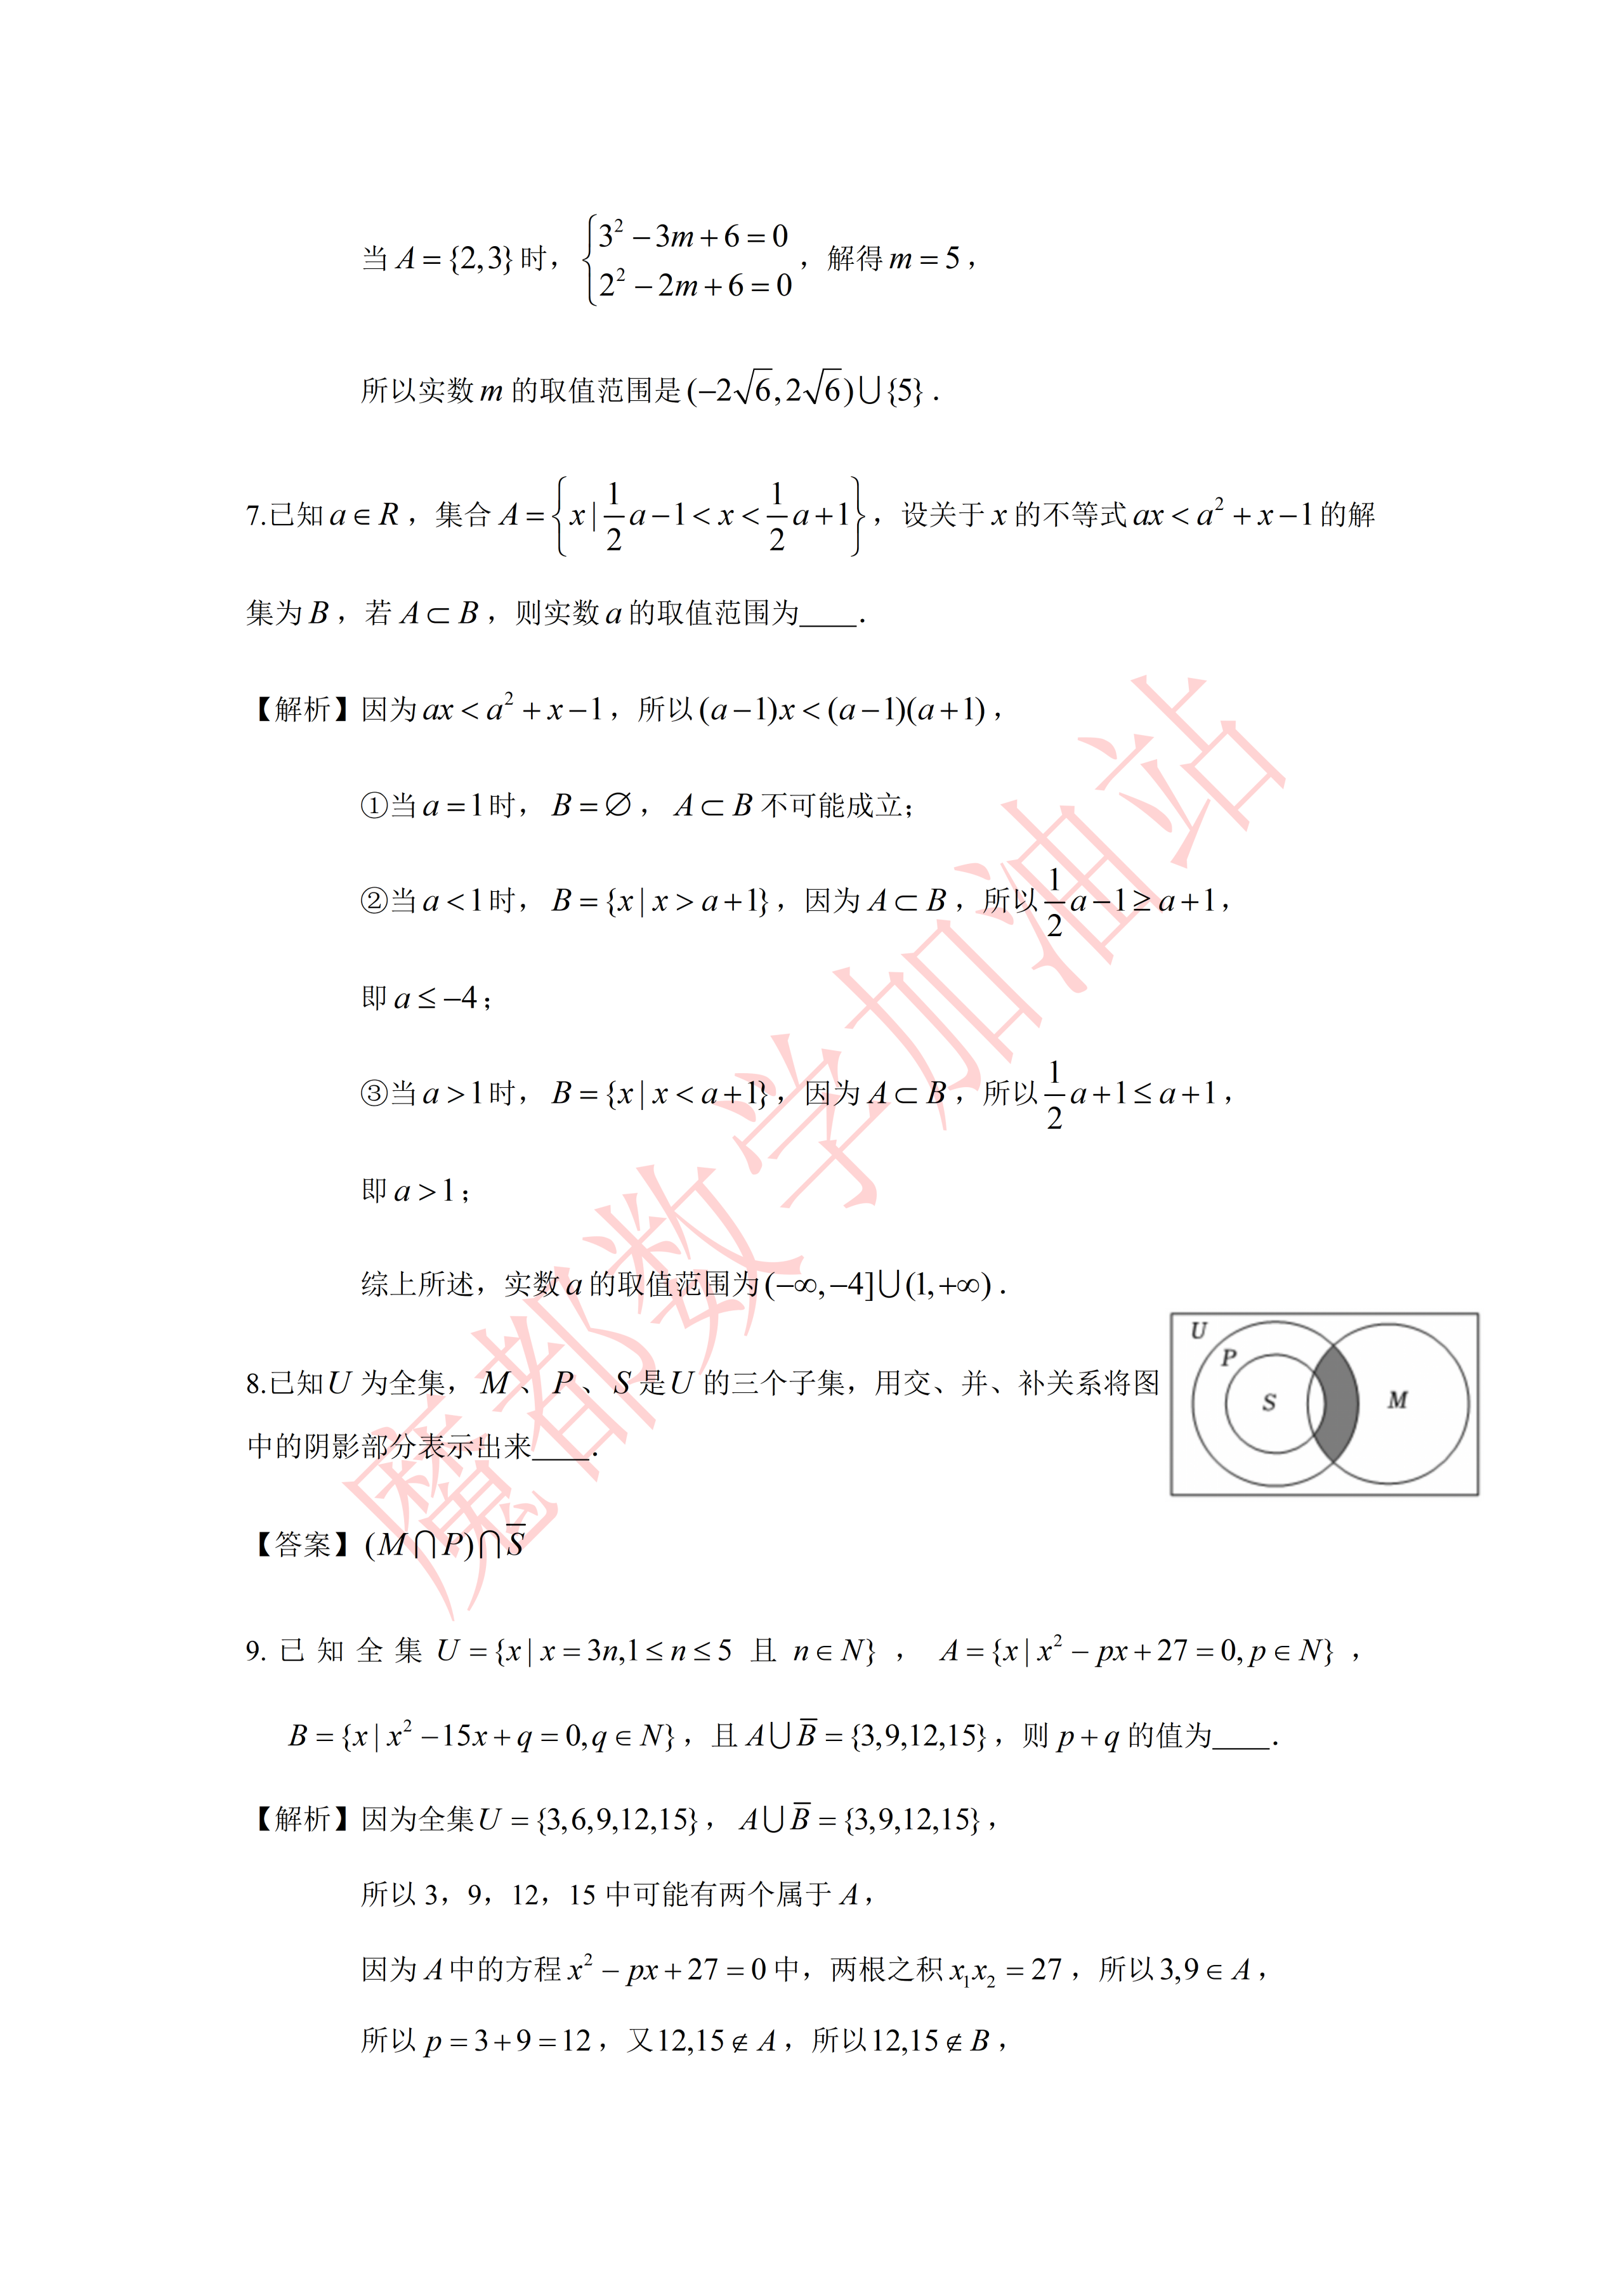
\includegraphics[width=.38\linewidth,trim=1835bp 1255bp 220bp 1565bp,clip]{../原图/高一49_华师大二附中_国庆作业1/02.png}
\end{center}

\ifanswer
\ans{$(M\cap P)\cap\overline S$}
\fi

\item 已知全集 $U=\{x\mid x=3n,1\leqslant n\leqslant5\text{ 且 }n\in\N\}$，$A=\{x\mid x^2-px+27=0,p\in\N\}$，$B=\{x\mid x^2-15x+q=0,q\in\N\}$，且 $A\cup\overline B=\{3,9,12,15\}$，则 $p+q$ 的值为\blankline[4.4em].

\ifanswer
\solbegin
\step{因为全集 $U=\{3,6,9,12,15\}$，$A\cup\overline B=\{3,9,12,15\}$，}
\step{所以 $3$、$9$、$12$、$15$ 中可能有两个属于 $A$，}
\step{因为 $A$ 中的方程 $x^2-px+27=0$ 中，两根之积 $x_1x_2=27$，所以 $3,9\in A$，}
\step{所以 $p=3+9=12$，又 $12,15\notin A$，所以 $12,15\notin B$，}
\step{因为 $B$ 中的方程 $x^2-15x+q=0$ 中，两根之和 $x_3+x_4=15$，所以 $6,9\in B$，}
\step{则 $q=6\times9=54$，所以 $p+q=66$.}
\solend
\fi

\item 已知集合 $A=\{x\mid x^2+(2a-3)x-3a=0,a\in\R,x\in\R\}$，集合 $B=\{x\mid x^2+(a-3)x+a^2-3a=0,a\in\R,x\in\R\}$，若 $A\neq B$，$A\cap B\neq\varnothing$，则 $A\cup B=$\blankline[4.4em].

\ifanswer
\solbegin
\step{设两个集合中的方程的公共解是 $b$，}
\step{由 $b^2+(2a-3)b-3a=b^2+(a-3)b+a^2-3a$，得 $ab=a^2$，}
\step{则 $a=0$ 或 $b=a$，}
\step{当 $a=0$ 时，不合题意，}
\step{当 $b=a$ 时，即两个方程的公共解为 $b=a$，}
\step{将 $b=a$ 代入方程，得 $a^2=2a$，$a=2$，}
\step{所以 $A=\{2,-3\}$，$B=\{-1,2\}$，所以 $A\cup B=\{-1,2,-3\}$.}
\solend
\fi

\item 已知一个有四个数字元素的集合 $S$，$S$ 的所有子集的元素和（空集的元素和认为是 $0$）的总和为 $16192$，则 $S$ 的元素之和等于\blankline[4.4em].

\ifanswer
\solbegin
\step{设 $S=\{a_1,a_2,a_3,a_4\}$，$S$ 的每个元素在所有子集中均出现 $2^3$ 次，}
\step{故 $(a_1+a_2+a_3+a_4)\cdot2^3=16192$，所以 $a_1+a_2+a_3+a_4=2024$，}
\step{故 $S$ 的元素之和等于 $2024$.}
\solend
\fi

\item 设 $P$ 为非空实数集满足：对任意给定的 $x,y\in P$（$x$、$y$ 可以相同），都有 $x+y\in P,x-y\in P,xy\in P$，则称 $P$ 为封闭集．关于封闭集有下列结论：

①集合 $P=\{-2,-1,0,1,2\}$ 为封闭集；

②集合 $P=\{x\mid x=2n,n\in\Z\}$ 为封闭集；

③若集合 $P_1$、$P_2$ 为封闭集，则 $P_1\cup P_2$ 为封闭集；

④若集合 $P$ 为封闭集，则一定有 $0\in P$；

⑤若集合 $P_1$、$P_2$ 为封闭集，则 $P_1\cap P_2$ 为封闭集.

其中正确结论的序号是\blankline[4.4em].

\ifanswer
\solbegin
\step{对于集合 $P=\{-2,-1,0,1,2\}$，取 $x=2$，$y=-2$，则 $x-y=2-(-2)=4\notin P$，}
\step{不满足封闭集的定义，所以①错误.}
\step{对于集合 $P=\{x\mid x=2n,n\in\Z\}$，设 $x=2n_1$，$y=2n_2$，$n_1,n_2\in\Z$.}
\step{$x+y=2n_1+2n_2=2(n_1+n_2)$，因为 $n_1+n_2\in\Z$，所以 $x+y\in P$.}
\step{$x-y=2n_1-2n_2=2(n_1-n_2)$，因为 $n_1-n_2\in\Z$，所以 $x-y\in P$.}
\step{$xy=2n_1\times2n_2=4n_1n_2=2(2n_1n_2)$，因为 $2n_1n_2\in\Z$，所以 $xy\in P$.}
\step{满足封闭集的定义，所以②正确.}
\step{令 $P_1=\{x\mid x=2n,n\in\Z\}$，$P_2=\{x\mid x=3n,n\in\Z\}$，都是封闭集.}
\step{$P_1\cup P_2$ 中，取 $x=2(x\in P_1)$，$y=3(y\in P_2)$，$x+y=5\notin P_1\cup P_2$，}
\step{不满足封闭集的定义，所以③错误.}
\step{因为对任意 $x\in P$，有 $x-x=0\in P$，}
\step{所以若集合 $P$ 为封闭集，则一定有 $0\in P$，所以④正确.}
\step{因为 $P_1$、$P_2$ 为封闭集，设 $x,y\in P_1\cap P_2$，则 $x,y\in P_1$ 且 $x,y\in P_2$.}
\step{因为 $P_1$ 是封闭集，所以 $x+y\in P_1,x-y\in P_1,xy\in P_1$.}
\step{因为 $P_2$ 是封闭集，所以 $x+y\in P_2,x-y\in P_2,xy\in P_2$.}
\step{所以 $x+y\in P_1\cap P_2,x-y\in P_1\cap P_2,xy\in P_1\cap P_2$，满足封闭集的定义，}
\step{所以⑤正确.}
\step{故正确的是②④⑤.}
\solend
\fi

\end{enumerate}

\bigsec{二、选择题}

\begin{enumerate}
\setcounter{enumi}{12}

\item 已知集合 $A=\{1,3,\sqrt m\}$，$B=\{1,m\}$，$B\subseteq A$，则 $m=$\mbox{（\quad）}

\keepwithprev
A. $0$ 或 $\sqrt3$\qquad B. $0$ 或 $3$

C. $1$ 或 $\sqrt3$\qquad D. $1$ 或 $3$

\ifanswer
\solbegin
\step{因为集合 $A=\{1,3,\sqrt m\}$，$B=\{1,m\}$，$B\subseteq A$，所以 $m=3$ 或 $m=\sqrt m$，}
\step{若 $m=3$，$A=\{1,3,\sqrt3\}$，$B=\{1,3\}$，满足 $B\subseteq A$，}
\step{若 $m=\sqrt m$，解得 $m=1$ 或 $m=0$，}
\step{①若 $m=0$，则 $A=\{1,3,0\}$，$B=\{1,0\}$，满足 $B\subseteq A$.}
\step{②若 $m=1$，则 $A$、$B$ 不满足集合中元素的互异性，舍去.}
\step{综上，$m=0$ 或 $m=3$．故选 $B$.}
\solend
\fi

\needvspace{10\baselineskip}

\item 设集合 $A$、$B$、$C$、$D$ 是全集 $X$ 的子集，$A\cap B\neq\varnothing$，$A\cap C\neq\varnothing$，则下列选项中正确的是\mbox{（\quad）}

\keepwithprev
A. 如果 $D\subset B$ 或 $D\subset C$，则 $D\cap A\neq\varnothing$

B. 如果 $D\subset A$，则 $\overline D\cap B\neq\varnothing$，$\overline D\cap C\neq\varnothing$

C. 如果 $A\subset D$，则 $\overline D\cap B=\varnothing$，$\overline D\cap C=\varnothing$

D. 上述各项都不正确

\ifanswer
\solbegin
\step{用韦恩图表示每个选项：}
\begin{center}
% 原图第 5 页解析配图（三联韦恩图）直接裁取（原卷排于选项 C、D 右侧）。
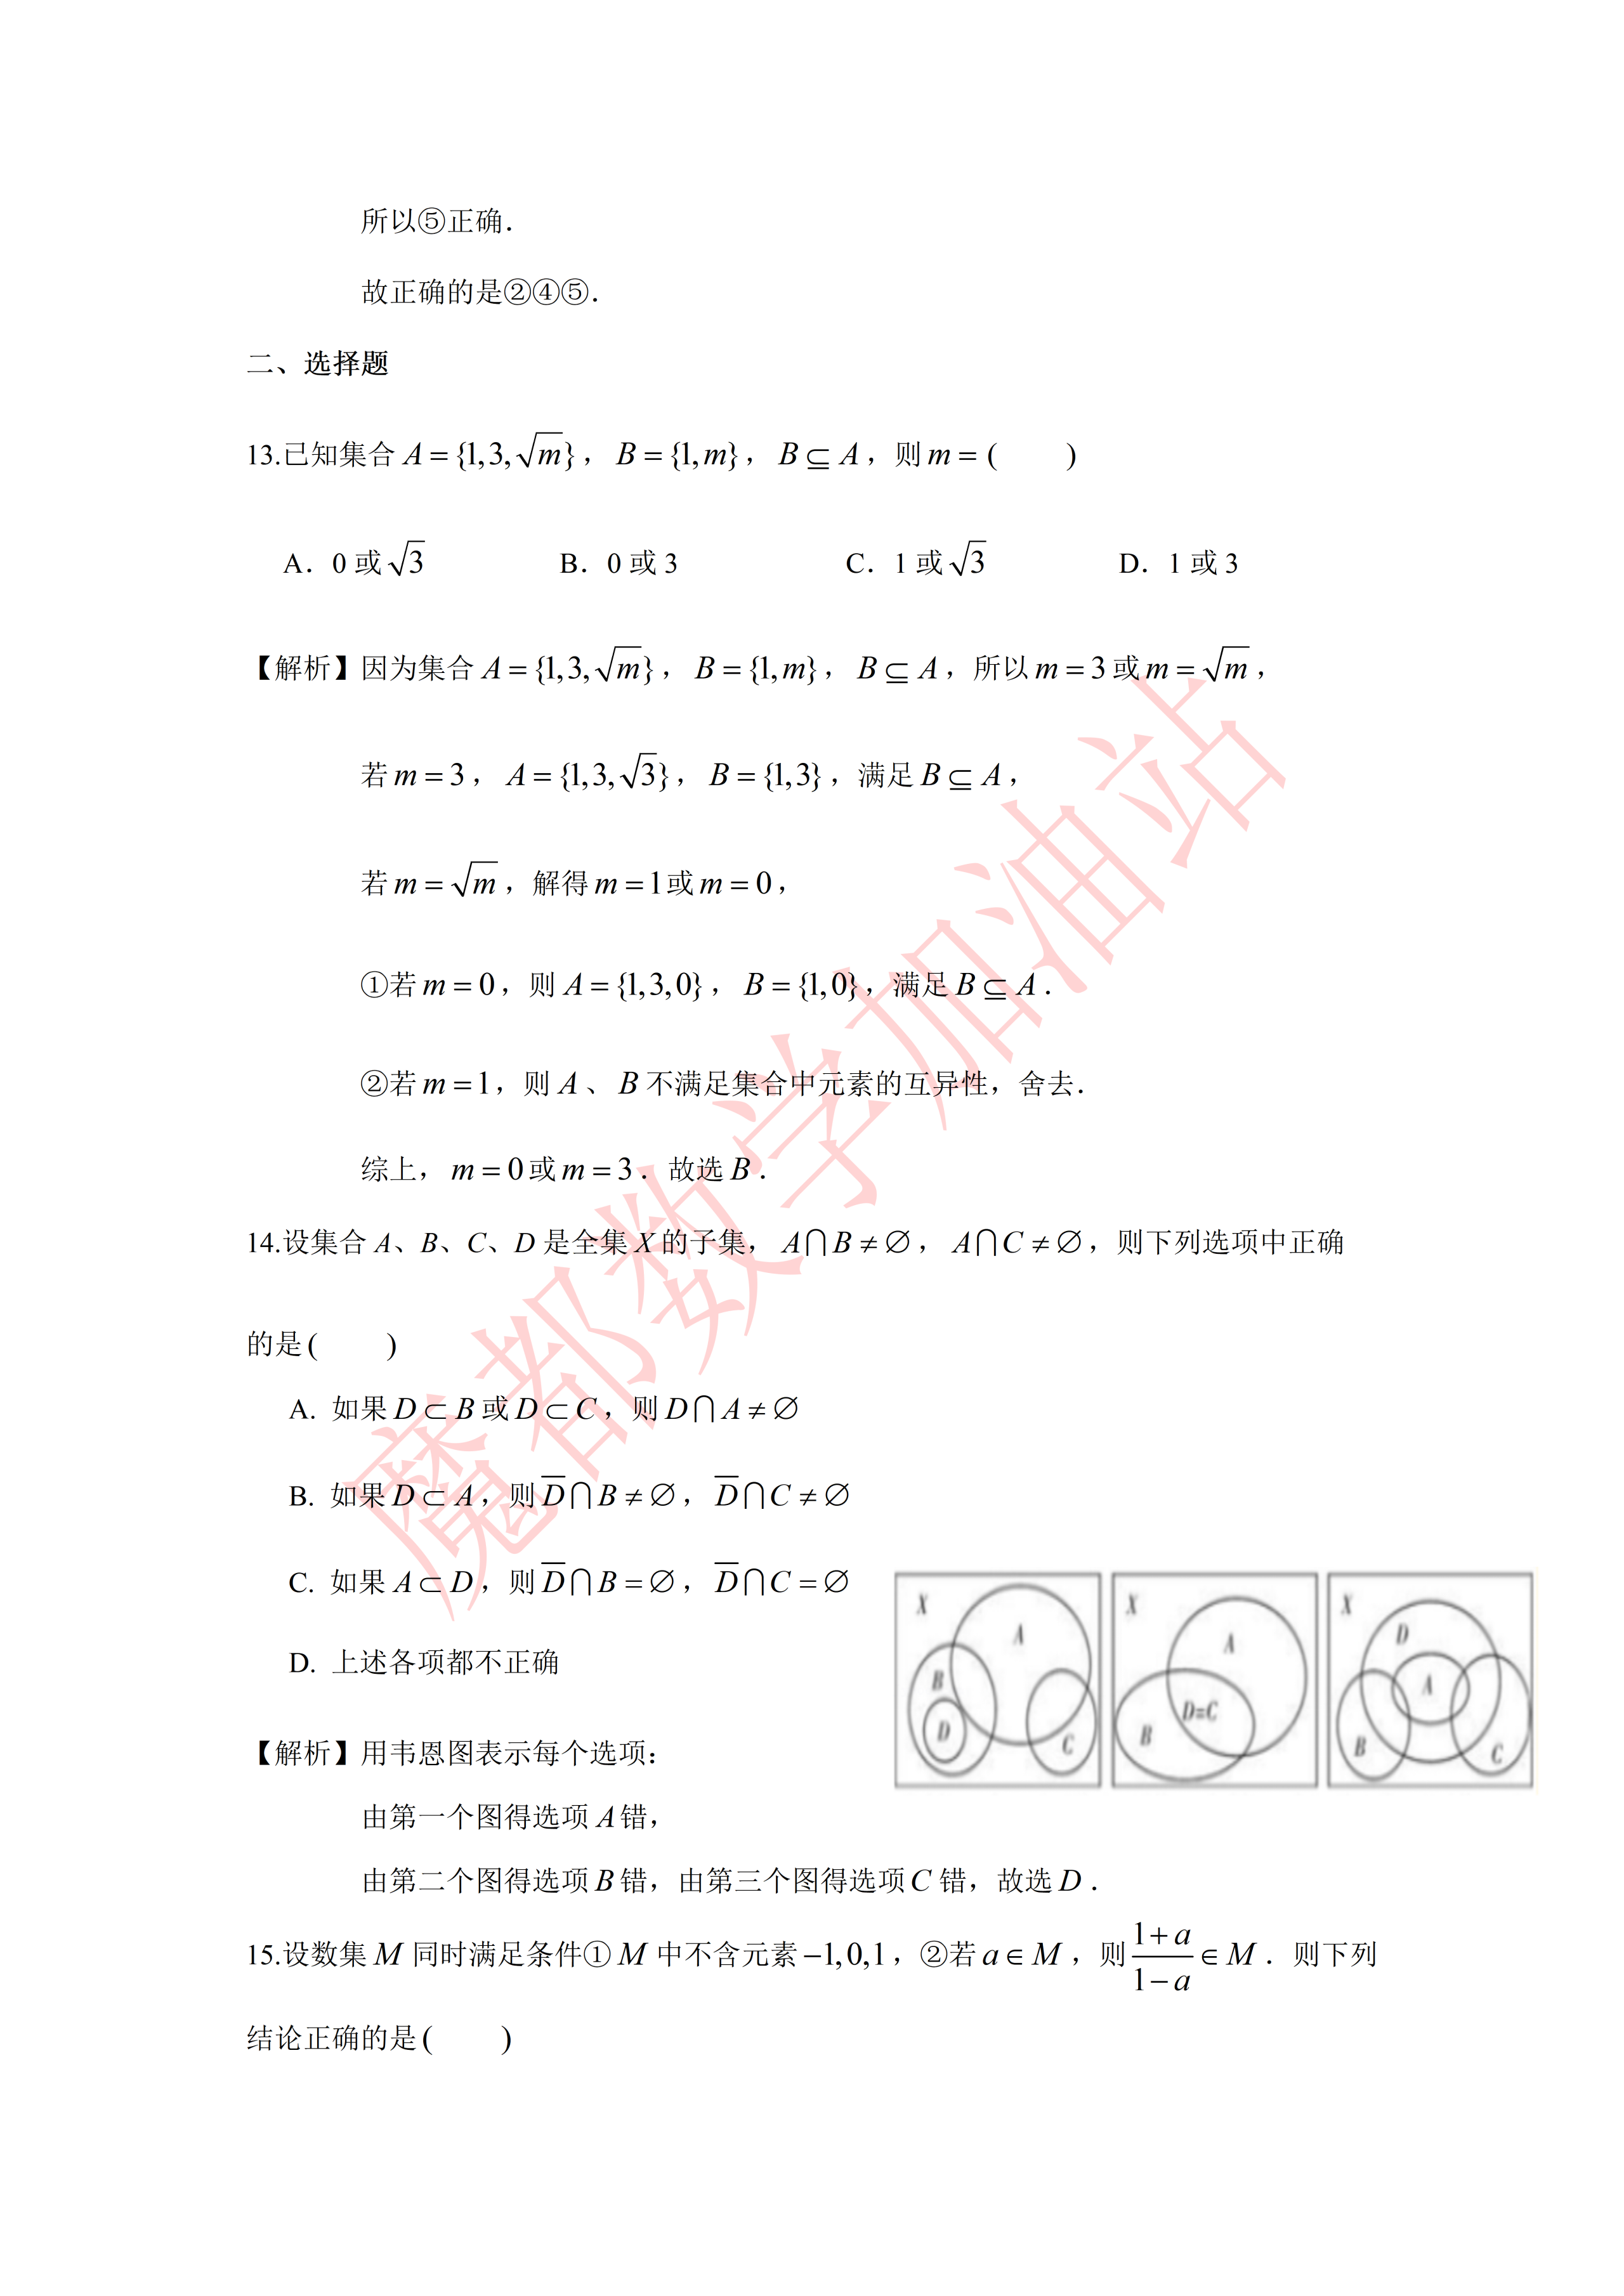
\includegraphics[width=.75\linewidth,trim=1400bp 790bp 135bp 1155bp,clip]{../原图/高一49_华师大二附中_国庆作业1/05.png}
\end{center}
\step{由第一个图得选项 $A$ 错，}
\step{由第二个图得选项 $B$ 错，由第三个图得选项 $C$ 错，故选 $D$.}
\solend
\fi

\item 设数集 $M$ 同时满足条件①$M$ 中不含元素 $-1$、$0$、$1$，②若 $a\in M$，则 $\dfrac{1+a}{1-a}\in M$．则下列结论正确的是\mbox{（\quad）}

\keepwithprev
A. 集合 $M$ 中至多有 $2$ 个元素\qquad B. 集合 $M$ 中至多有 $3$ 个元素

C. 集合 $M$ 中有且仅有 $4$ 个元素\qquad D. 集合 $M$ 中有无穷多个元素

\ifanswer
\solbegin
\step{若集合只含有一个元素，则 $\dfrac{1+a}{1-a}=a$，即 $1+a=a-a^2$，即 $-a^2=1$，不成立.}
\step{当 $a=3$ 时，$\dfrac{1+3}{1-3}=-2\in M$，所以 $\dfrac{1-2}{1+2}=-\dfrac13\in M$，所以 $\dfrac{1-\frac13}{1+\frac13}=\dfrac12\in M$，}
\step{所以 $\dfrac{1+\frac12}{1-\frac12}=3$，开始重复了，所以 $M=\left\{3,-2,-\dfrac13,\dfrac12\right\}$；}
\step{当 $a=2$ 时，$\dfrac{1+2}{1-2}=-3\in M$，所以 $\dfrac{1-3}{1+3}=-\dfrac12\in M$，所以 $\dfrac{1-\frac12}{1+\frac12}=\dfrac13\in M$，}
\step{所以 $\dfrac{1+\frac13}{1-\frac13}=2$，开始重复了，所以 $M=\left\{2,-3,-\dfrac12,-\dfrac13\right\}$，}
\step{此时也只要四个元素；}
\step{当 $a=\dfrac34\in M$，则 $7\in M$，若 $7\in M$，则 $-\dfrac43\in M$，}
\step{若 $-\dfrac43\in M$，则 $-\dfrac17\in M$，若 $-\dfrac17\in M$，有 $\dfrac34\in M$，}
\step{由归纳推理得，集合 $M$ 中有且仅有 $4$ 个元素．故选 $C$.}
\solend
\fi

\item 已知集合 $M=\{x\mid x\in\N,0<x\leqslant15\}$，$A_1$、$A_2$、$A_3$ 满足：①$A_1\cup A_2\cup A_3=M$；②每个集合都恰有 $5$ 个元素．集合 $A_i$（$i=1,2,3$）中最大元素与最小元素之和称为 $A_i$ 的特征数，记为 $X_i$（$i=1,2,3$），则 $X_1+X_2+X_3$ 的值不可能为\mbox{（\quad）}

\keepwithprev
A. $37$\qquad B. $39$\qquad C. $48$\qquad D. $57$

\ifanswer
\solbegin
\step{因为集合 $M=\{x\mid x\in\N,0<x\leqslant15\}=\{1,2,3,\cdots,15\}$，}
\step{又因为集合 $A_1$、$A_2$、$A_3$ 中，每个集合恰有 $5$ 个元素，}
\step{且 $A_1\cup A_2\cup A_3=M$ 有 $15$ 个元素，所以集合 $A_1$、$A_2$、$A_3$ 中没有重复元素，}
\step{因为 $1$ 是集合 $M$ 中数值最小的元素，$15$ 是集合 $M$ 中数值最大的元素，}
\step{所以在 $A_i$ 的特征数构成中，必有 $1$ 和 $15$，不妨设 $1\in A_1$，$15\in A_1$，}
\step{要使 $X_1+X_2+X_3$ 最大，则应该在集合 $A_1$ 中首先放置数值较小的元素，}
\step{即 $A_1=\{1,2,3,4,15\}$，所以 $5$ 与 $14$ 是剩下元素中数值最小或最大的元素，}
\step{同理，不妨设 $5\in A_2$，$14\in A_2$，接着在 $A_2$ 中再次放置数值较小的元素，}
\step{即 $A_2=\{5,6,7,8,14\}$，则 $A_3=\{9,10,11,12,13\}$，}
\step{此时 $X_1+X_2+X_3$ 有最大值为 $1+15+5+14+9+13=57$，}
\step{即 $X_1+X_2+X_3\leqslant57$；}
\step{要使 $X_1+X_2+X_3$ 最小，则在集合 $A_1$ 中首先放置数值较大的元素，}
\step{即 $A_1=\{1,12,13,14,15\}$，所以 $2$ 与 $11$ 是剩下元素中数值最小或最大的元素，}
\step{同理，不妨设 $2\in A_2$，$11\in A_2$，接着在 $A_2$ 中再次放置数值较大的元素，}
\step{即 $A_2=\{2,8,9,10,11\}$，则 $A_3=\{3,4,5,6,7\}$，}
\step{此时 $X_1+X_2+X_3$ 有最小值为 $1+15+2+11+3+7=39$，}
\step{即 $X_1+X_2+X_3\geqslant39$，}
\step{综上，$39\leqslant X_1+X_2+X_3\leqslant57$，故选 $A$.}
\solend
\fi

\end{enumerate}

\bigsec{三、解答题}

\begin{enumerate}
\setcounter{enumi}{16}

\item 已知全集为 $\R$，集合 $A=\{x\mid y=\sqrt{(2+x)(4-x)}\}$，$B=\{x\mid-1<x<m+1\}$.

\begin{enumerate}[label=(\arabic*)]
\item 若 $m=4$，求 $A\cup B$、$\overline A\cap B$；
\item 若 $B\subseteq A$，求实数 $m$ 的取值范围.
\end{enumerate}

\ifanswer
\solbegin
\stepm{(1)}{集合 $A=\{x\mid y=\sqrt{(2+x)(4-x)}\}=\{x\mid-2\leqslant x\leqslant4\}$，}
\step{当 $m=4$ 时，$B=\{x\mid-1<x<5\}$.}
\step{所以 $A\cup B=[-2,5)$，$\overline A=\{x\mid x<-2\text{ 或 }x>4\}$，$\overline A\cap B=(4,5)$.}
\stepm{(2)}{因为 $B\subseteq A$，}
% 原卷如此，照录未改（第 17 题(2)解析两处"当 C=∅／当 C≠∅"应为 B，本卷并无集合 C）
\step{当 $C=\varnothing$ 时，$m\leqslant-2$，$B\subseteq A$ 成立；}
\step{当 $C\neq\varnothing$ 时，$m>-2$，$-1<m+1\leqslant4$，解得 $-2<m\leqslant3$，}
\step{综上，$m\leqslant3$，所以实数 $m$ 的取值范围是 $(-\infty,3]$.}
\solend
\fi

\ansspace[6]

\item 用反证法证明：若 $a$、$b$、$c\in\R$，且 $x=a^2-2b+1$，$y=b^2-2c+1$，$z=c^2-2a+1$，则 $x$、$y$、$z$ 中至少有一个不小于 $0$.

\ifanswer
\solbegin
\step{假设 $x$、$y$、$z$ 均小于 $0$，即 $x=a^2-2b+1<0$①，$y=b^2-2c+1<0$②，}
\step{$z=c^2-2a+1<0$③，①$+$②$+$③得 $x+y+z=(a-1)^2+(b-1)^2+(c-1)^2<0$，}
\step{这与 $(a-1)^2+(b-1)^2+(c-1)^2\geqslant0$ 矛盾，则假设不成立，}
\step{所以 $x$、$y$、$z$ 中至少有一个不小于 $0$，得证.}
\solend
\fi

\ansspace[5]

\item 已知全集为 $\R$，实数 $a$、$b$ 满足 $a\neq b$，集合 $M=\{x\mid x^2-3x-4\leqslant0\}$，集合 $A=\{x\mid(x+a)(x+b)>0\}$，集合 $B=\{x\mid x^2+(a-2)x-2a>0\}$.

\begin{enumerate}[label=(\arabic*)]
\item 若 $\overline A=M$，求 $a$、$b$ 的值；
\item 若 $a>b>-1$，求 $A\cap B$；
\item 若 $a^2+a\in\overline B$，求 $a$ 的取值范围.
\end{enumerate}

\ifanswer
\solbegin
\stepm{(1)}{$M=\{x\mid x^2-3x-4\leqslant0\}=\{x\mid-1\leqslant x\leqslant4\}$，$A=\{x\mid(x+a)(x+b)\leqslant0\}$，}
\step{因为 $\overline A=M$，所以 $a=1$，$b=-4$ 或 $a=-4$，$b=1$.}
\stepm{(2)}{因为 $a>b>-1$，所以 $-a<-b<1$，所以 $A=\{x\mid x<-a\text{ 或 }x>-b\}$，}
\step{因为 $B=\{x\mid x^2+(a-2)x-2a>0\}=\{x\mid x<-a\text{ 或 }x>2\}$，}
\step{所以 $A\cap B=\{x\mid x<-a\text{ 或 }x>2\}$，}
\stepm{(3)}{$\overline B=\{x\mid(x-2)(x+a)\leqslant0\}$，}
% 原卷如此，照录未改（第 19 题(3)此处"a(a-1)((a-2)^2≤0"括号不配对；且由左式展开应为
% a(a-1)(a+2)^2≤0，与下句"解得 a=2 …[0,1]∪{2}"按 (a-2)^2 方自洽，见文件头清单第 2 条）
\step{由 $a^2+a\in\overline B$，得 $(a^2+a-2)(a^2+2a)\leqslant0\Leftrightarrow a(a-1)((a-2)^2\leqslant0$，}
\step{解得 $a=2$ 或 $0\leqslant a\leqslant1$，故 $a$ 的取值范围是 $[0,1]\cup\{2\}$.}
\solend
\fi

\ansspace[7]

\item 设数集 $A$ 由实数构成，若 $x\in A$（$x\neq1$ 且 $x\neq0$），则 $\dfrac{1}{1-x}\in A$.

\begin{enumerate}[label=(\arabic*)]
\item 若 $2\in A$，则 $A$ 中至少还有几个元素；
\item 集合 $A$ 是否为双元素集合？请说明理由；
\item 若 $A$ 中元素个数不超过 $8$ 个，所有元素的和为 $\dfrac{14}{3}$，且 $A$ 中有一个元素的平方等于所有元素的积，求集合 $A$.
\end{enumerate}

\ifanswer
\solbegin
\stepm{(1)}{若 $x\in A$，则 $\dfrac{1}{1-x}\in A$，又 $2\in A$，所以 $\dfrac{1}{1-2}=-1\in A$，}
\step{所以 $\dfrac{1}{1-(-1)}=\dfrac12\in A$，所以 $\dfrac{1}{1-\frac12}=2\in A$，}
% 原卷如此，照录未改（第 20 题(1)解析末句"2 个几个元素"衍一"几个"）
\step{所以 $A$ 中至少还有 $2$ 个几个元素；}
\stepm{(2)}{若 $x\in A$（$x\neq1$ 且 $x\neq0$），则 $\dfrac{1}{1-x}\in A$，}
\step{则 $\dfrac{1}{1-\frac{1}{1-x}}=\dfrac{1-x}{-x}\in A$，则 $\dfrac{1}{1-\frac{1-x}{-x}}=x\in A$}
\step{若 $A$ 为双元素集，则 $x=\dfrac{1}{1-x}$ 或 $x=\dfrac{1-x}{-x}$ 或 $\dfrac{1}{1-x}=\dfrac{1-x}{-x}$，均无解，}
\step{所以 $A$ 不可能为双元素集；}
\stepm{(3)}{由 $x\in A$，$\dfrac{1}{1-x}\in A$，得 $\dfrac{1}{1-\frac{1}{1-x}}=\dfrac{x-1}{x}\in A$，得 $\dfrac{1}{1-\frac{x-1}{x}}=x\in A$，}
\step{所以 $\left\{x,\dfrac{1}{1-x},\dfrac{x-1}{x}\right\}\subseteq A$，而 $x\cdot\dfrac{1}{1-x}\cdot\dfrac{x-1}{x}=-1$，}
\step{$A$ 中元素个数为 $3$ 的倍数，则 $A$ 中元素只有 $6$ 个，}
\step{因为 $A$ 中有一个元素的平方等于所有元素的积，}
\step{不妨设 $x^2=1$，解得 $x=-1$ 或 $x=1$（舍），则 $-1$、$\dfrac12$、$2\in A$，}
\step{所以 $-1+\dfrac12+2+m+\dfrac{1}{1-m}+\dfrac{m-1}{m}=\dfrac{14}{3}$，解得 $m=-\dfrac12$ 或 $m=3$ 或 $m=\dfrac23$，}
\step{所以 $A=\left\{\dfrac12,2,-1,-\dfrac12,3,\dfrac23\right\}$.}
\solend
\fi

\ansspace[9]

% 原卷如此，照录未改（第 21 题题干"21.求已知集合"之"求"字疑衍；"任意两个元素 a_i a_j"
% 疑脱逗号；"|a_i-a_j|≥1/30 则称"之前疑脱标点，见文件头清单第 4 条）
\item 求已知集合 $M=\left\{\dfrac{1}{k}\middle|1\leqslant k\leqslant100\text{ 且 }k\in\N^{*}\right\}$，$A=\{a_1,a_2,\cdots,a_n\}$，其中 $n\in\N^{*}$，且 $n\geqslant2$．若 $A\subseteq\N$，且对集合 $A$ 中的任意两个元素 $a_ia_j$，$i\neq j$ 都有 $|a_i-a_j|\geqslant\dfrac{1}{30}$ 则称集合 $A$ 有性质 $P$.

\begin{enumerate}[label=(\arabic*)]
\item 判断集合 $\left\{\dfrac13,\dfrac14,\dfrac15,\dfrac16,\dfrac17\right\}$ 是否具有性质 $P$；
\item 若集合 $A=\{a_1,a_2,\cdots,a_n\}$ 具有性质 $P$.

①求证：$a_i-a_j$ 的最大值大于等于 $\dfrac{n-1}{30}$；

②求 $A$ 的元素个数 $n$ 的最大值.
\end{enumerate}

\ifanswer
\solbegin
\stepm{(1)}{集合为 $\left\{\dfrac13,\dfrac14,\dfrac15,\dfrac16,\dfrac17\right\}$，又 $\dfrac16-\dfrac17=\dfrac{1}{42}<\dfrac{1}{30}$，所以该集合不具有性质 $P$；}
\stepm{(2)}{①因为集合 $A=\{a_1,a_2,\cdots,a_n\}$ 具有性质 $P$，}
\step{不妨设 $a_1<a_2<a_3<\cdots<a_n$，则 $a_i-a_j\geqslant\dfrac{1}{30}$（$i>j$），}
\step{所以 $a_n-a_1=(a_n-a_{n-1})+(a_{n-1}-a_{n-2})+\cdots+(a_2-a_1)\geqslant\dfrac{n-1}{30}$，}
\step{故 $a_i-a_j$ 的最大值大于等于 $\dfrac{n-1}{30}$；}
% 原卷如此，照录未改（第 21 题(2)②首行"a_2-a_1≥(n-1)/30"：由①同款推理只能得
% a_2-a_1≥1/30，见文件头清单第 5 条）
\step{②$A=\{a_1,a_2,\cdots,a_n\}$，不妨设 $a_1<a_2<a_3<\cdots<a_n$，}
\step{要使 $A$ 的元素个数 $n$ 最大，}
\step{则 $A$ 中的元素满足 $a_n=\dfrac{1}{k}$，$a_{n-1}=\dfrac{1}{k+1}$，$\cdots$，$a_1=\dfrac{1}{k+n-1}$（$k\in\N^{*}$），}
\step{又由①得 $a_2-a_1=\dfrac{1}{k+n-2}-\dfrac{1}{k+n-1}\geqslant\dfrac{n-1}{30}$，}
\step{所以 $(k+n-2)(k+n-1)\leqslant30$，又 $a_n-a_{n-1}=\dfrac{1}{k}-\dfrac{1}{k+1}\geqslant\dfrac{1}{30}$，}
\step{所以 $k(k+1)\leqslant30$，所以 $1\leqslant k\leqslant5$（$k\in\N^{*}$），}
\step{当 $k=5$ 时，由 $(k+n-2)(k+n-1)\leqslant30$，解得 $n\leqslant2$，$n\in\N^{*}$；}
\step{当 $k=4$ 时，由 $(k+n-2)(k+n-1)\leqslant30$，解得 $n\leqslant3$，$n\in\N^{*}$；}
\step{当 $k=3$ 时，由 $(k+n-2)(k+n-1)\leqslant30$，解得 $n\leqslant4$，$n\in\N^{*}$；}
\step{当 $k=2$ 时，由 $(k+n-2)(k+n-1)\leqslant30$，解得 $n\leqslant5$，$n\in\N^{*}$；}
\step{当 $k=1$ 时，由 $(k+n-2)(k+n-1)\leqslant30$，解得 $n\leqslant6$，$n\in\N^{*}$.}
\step{故 $A$ 的元素个数 $n$ 的最大值为 $6$，此时集合 $A=\left\{1,\dfrac12,\dfrac13,\cdots,\dfrac16\right\}$.}
\solend
\fi

\ansspace*[10]

\end{enumerate}

\end{document}
"
% 紧凑版：xelatex "\def\iscompact{1}% 高一49_华师大二附中_国庆作业1.tex
%   —— 高一上数学"2026-2027 年华师大二附中高一上国庆作业 1"（讲评版）
% 试卷版：xelatex 高一49_华师大二附中_国庆作业1.tex
% 答案版：xelatex "\def\isanswer{1}\input{高一49_华师大二附中_国庆作业1.tex}"
% 紧凑版：xelatex "\def\iscompact{1}\input{高一49_华师大二附中_国庆作业1.tex}"
%
% 原始材料：微信公众号"魔都数学加油站"文章，作者破晓，连载"27学年高一49"；
% 原文标题"27学年高一49——2026-2027年上海市华师大二附中高一上国庆作业1集合与逻辑、
% 等式与不等式的性质"；页面用 JS 渲染，未见明确发布日期（页内时间戳 ≈ 2026-10-05 21:37）；
% 原文链接：https://mp.weixin.qq.com/s/XxZTOBVQslK5cZm2_BbhOg。
% 正文为 11 张 PNG 页：第 01、03、04、06、07、08、09 页 4762×6735，
% 第 02、05、10、11 页 2560×3620，均按页序读取；粉色斜排"魔都数学加油站"为卷面水印，
% 与公众号页脚一并未录入。全卷 11 页均为试卷页，无二维码/宣传页。
%
% 题号与分节：原文自第 3 题起编，填空题 3—12、选择题 13—16、解答题 17—21，共 19 题。
% 讲评版：原卷每题下直接印【答案】或【解析】——只印【答案】的 3 题（第 3、5、8 题），
% 其余 16 题均只印【解析】；解析行数已逐题按印刷行照录（一条 \step＝原卷一个印刷行）。
%
% 卷首标题：照卷面印作"2026-2027 年华师大二附中高一上国庆作业 1"（公众号标题中的"上海市"
% 卷面没有，本稿照卷面），年份区间按全稿惯例排 en dash；副标题照卷面自印的
% "集合与逻辑单元综合检测"（原卷页首标题行下方即印此行，故不另按模块口径拟名）。
% 副标题依据：全卷 19 题均为集合与常用逻辑用语内容——集合类 15 题（6—17、19—21 中除
% 反证法题外），逻辑/命题类 3 题（第 3 题否定形式、第 4 题充要条件、第 5 题反证法假设），
% 反证法证明 1 题（第 18 题）；全卷无不等式求解题，公众号标题中"等式与不等式的性质"
% 与卷面实际内容不符。
%
% 与原卷的排版差异：
%   ① 原文从第 3 题起，填空题为 3—12、选择题为 13—16、解答题为 17—21，本稿保留原题号；
%   ② 原卷每题下直接印【答案】/【解析】，本稿按全稿惯例置于答案版；只印【解析】的题
%      不另提 \ans{}（照 高一36 口径），只印【答案】的题仅给 \ans{}；
%   ③ 原卷第 8 题韦恩图排在题干右侧、第 14 题三联韦恩图排在选项（C、D）右侧，
%      本稿分别移至题干下方、解析首步之后居中排，均直接裁取原图页（02.png、05.png）；
%   ④ 数集记号原卷排作斜体/加粗 R、N、Z，本稿统一为 \R、\N、\Z、\N^*；
%      填空横线按全稿惯例排为 \blankline[4.4em]。
%
% 原卷笔误/存疑清单（均照录未改，正文中该处有 % 注）：
%   1. 第 17 题(2)解析两处"当 C=∅／当 C≠∅"应为 B（本卷并无集合 C）；
%   2. 第 19 题(3)解析"a(a-1)((a-2)^2≤0"括号不配对（多一枚左括号）；且由
%      (a^2+a-2)(a^2+2a)≤0 展开应为 a(a-1)(a+2)^2≤0，与原卷结论"解得 a=2 …
%      [0,1]∪{2}"恰按 (a-2)^2 自洽——因式分解与原式不符，结论按 (a-2)^2 自洽，均照录；
%   3. 第 20 题(1)解析末句"至少还有 2 个几个元素"衍一"几个"；
%   4. 第 21 题题干"21.求已知集合"之"求"字疑衍；"任意两个元素 a_i a_j"疑脱逗号；
%      "≥1/30 则称"之前疑脱标点；
%   5. 第 21 题(2)②解析"a_2-a_1≥(n-1)/30"：由①同款推理只能得 a_2-a_1≥1/30，
%      原卷如此，照录未改（后续 (k+n-2)(k+n-1)≤30 即按该行推得）。
%
\documentclass[a4paper,11pt]{article}
\usepackage{common}

\begin{document}

\examtitlest[3]{2026--2027 年华师大二附中高一上国庆作业 1}{集合与逻辑单元综合检测}

\bigsec{一、填空题}

\begin{enumerate}
\setcounter{enumi}{2}

\item “若 $x^2-x-2\leqslant0$，则 $-1\leqslant x\leqslant2$”的否定形式为\blankline[4.4em].

\ifanswer
\ans{若 $x^2-x-2>0$，则 $x<-1$ 或 $x>2$}
\fi

\item 已知 $p:|x-3|<5$，$q:1-a<x<2a-3$，且 $p$ 是 $q$ 的充分非必要条件，则实数 $a$ 的取值范围是\blankline[4.4em].

\ifanswer
\solbegin
\step{由 $|x-3|<5$ 得 $-2<x<8$，}
\step{又 $p$ 是 $q$ 的充分不必要条件，所以 $(-2,8)\subset(1-a,2a-3)$，}
\step{即 $\begin{cases}-2\geqslant1-a\\ 8\leqslant2a-3\\ (2a-3)-(1-a)\neq8-(-2)\end{cases}$，解得 $a\geqslant\dfrac{11}{2}$，实数 $a$ 的取值范围是 $\left[\dfrac{11}{2},+\infty\right)$.}
\solend
\fi

\item 用反证法证明命题“设 $a$、$b\in\R$，则方程 $a_1x^2+b_1x+c_1=0$ 与 $a_2x^2+b_2x+c_2=0$ 至少有一个实根”时要做的假设是\blankline[4.4em].

\ifanswer
\ans{假设 $a$、$b\in\R$，方程 $a_1x^2+b_1x+c_1=0$ 与 $a_2x^2+b_2x+c_2=0$ 都没有实根}
\fi

\item 设集合 $A=\{x\mid x^2-mx+6=0,x\in\R\}$，且 $A\cap\{2,3\}=A$，则实数 $m$ 的取值范围是\blankline[4.4em].

\ifanswer
\solbegin
\step{由 $A\cap\{2,3\}=A$，得 $A\subseteq\{2,3\}$，}
\step{当 $A=\varnothing$ 时，$\Delta=m^2-24<0$，解得 $-2\sqrt6<m<2\sqrt6$；}
\step{当 $A=\{2\}$ 时，$\begin{cases}2^2-2m+6=0\\ \Delta=m^2-24=0\end{cases}$，无解；}
\step{当 $A=\{3\}$ 时，$\begin{cases}3^2-3m+6=0\\ \Delta=m^2-24=0\end{cases}$，无解；}
\step{当 $A=\{2,3\}$ 时，$\begin{cases}3^2-3m+6=0\\ 2^2-2m+6=0\end{cases}$，解得 $m=5$，}
\step{所以实数 $m$ 的取值范围是 $(-2\sqrt6,2\sqrt6)\cup\{5\}$.}
\solend
\fi

\item 已知 $a\in\R$，集合 $A=\left\{x\middle|\dfrac12a-1<x<\dfrac12a+1\right\}$，设关于 $x$ 的不等式 $ax<a^2+x-1$ 的解集为 $B$，若 $A\subset B$，则实数 $a$ 的取值范围为\blankline[4.4em].

\ifanswer
\solbegin
\step{因为 $ax<a^2+x-1$，所以 $(a-1)x<(a-1)(a+1)$，}
\step{①当 $a=1$ 时，$B=\varnothing$，$A\subset B$ 不可能成立；}
\step{②当 $a<1$ 时，$B=\{x\mid x>a+1\}$，因为 $A\subset B$，所以 $\dfrac12a-1\geqslant a+1$，}
\step{即 $a\leqslant-4$；}
\step{③当 $a>1$ 时，$B=\{x\mid x<a+1\}$，因为 $A\subset B$，所以 $\dfrac12a+1\leqslant a+1$，}
\step{即 $a>1$；}
\step{综上所述，实数 $a$ 的取值范围为 $(-\infty,-4]\cup(1,+\infty)$.}
\solend
\fi

\needvspace{8\baselineskip}

\item 已知 $U$ 为全集，$M$、$P$、$S$ 是 $U$ 的三个子集，用交、并、补关系将图中的阴影部分表示出来\blankline[4.4em].

\begin{center}
% 原图第 2 页题旁韦恩图直接裁取（原卷排于题干右侧）。
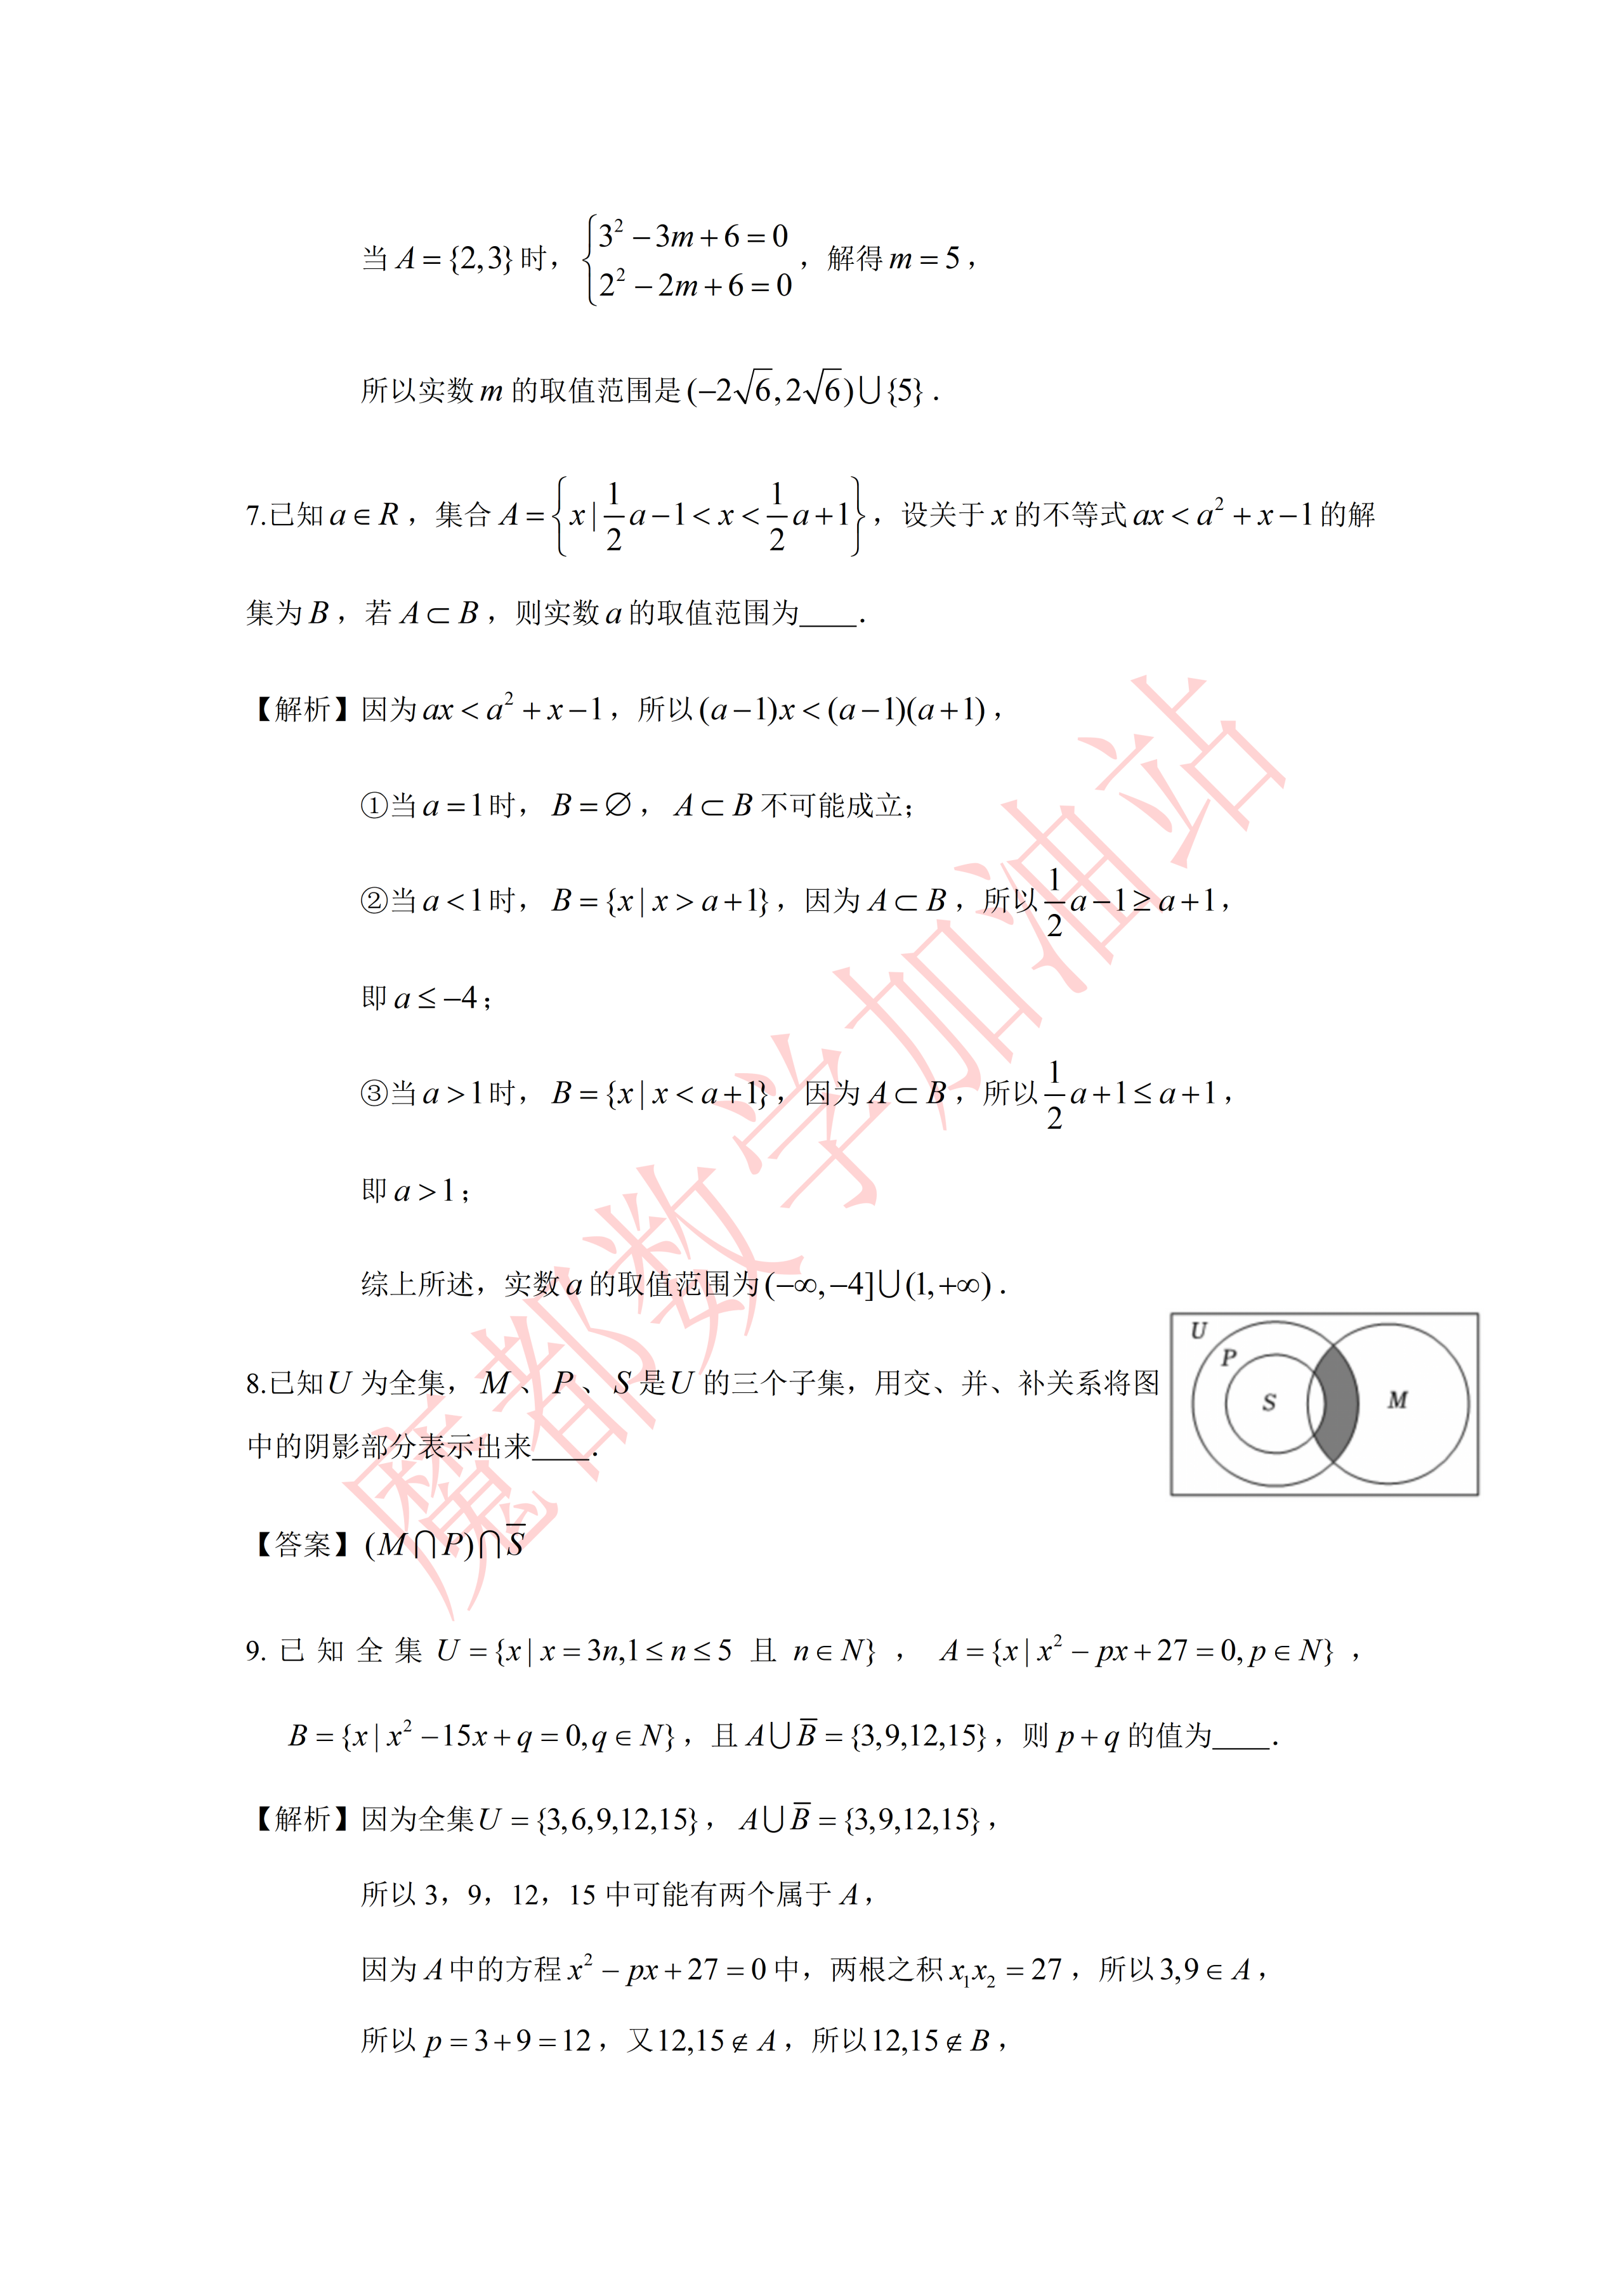
\includegraphics[width=.38\linewidth,trim=1835bp 1255bp 220bp 1565bp,clip]{../原图/高一49_华师大二附中_国庆作业1/02.png}
\end{center}

\ifanswer
\ans{$(M\cap P)\cap\overline S$}
\fi

\item 已知全集 $U=\{x\mid x=3n,1\leqslant n\leqslant5\text{ 且 }n\in\N\}$，$A=\{x\mid x^2-px+27=0,p\in\N\}$，$B=\{x\mid x^2-15x+q=0,q\in\N\}$，且 $A\cup\overline B=\{3,9,12,15\}$，则 $p+q$ 的值为\blankline[4.4em].

\ifanswer
\solbegin
\step{因为全集 $U=\{3,6,9,12,15\}$，$A\cup\overline B=\{3,9,12,15\}$，}
\step{所以 $3$、$9$、$12$、$15$ 中可能有两个属于 $A$，}
\step{因为 $A$ 中的方程 $x^2-px+27=0$ 中，两根之积 $x_1x_2=27$，所以 $3,9\in A$，}
\step{所以 $p=3+9=12$，又 $12,15\notin A$，所以 $12,15\notin B$，}
\step{因为 $B$ 中的方程 $x^2-15x+q=0$ 中，两根之和 $x_3+x_4=15$，所以 $6,9\in B$，}
\step{则 $q=6\times9=54$，所以 $p+q=66$.}
\solend
\fi

\item 已知集合 $A=\{x\mid x^2+(2a-3)x-3a=0,a\in\R,x\in\R\}$，集合 $B=\{x\mid x^2+(a-3)x+a^2-3a=0,a\in\R,x\in\R\}$，若 $A\neq B$，$A\cap B\neq\varnothing$，则 $A\cup B=$\blankline[4.4em].

\ifanswer
\solbegin
\step{设两个集合中的方程的公共解是 $b$，}
\step{由 $b^2+(2a-3)b-3a=b^2+(a-3)b+a^2-3a$，得 $ab=a^2$，}
\step{则 $a=0$ 或 $b=a$，}
\step{当 $a=0$ 时，不合题意，}
\step{当 $b=a$ 时，即两个方程的公共解为 $b=a$，}
\step{将 $b=a$ 代入方程，得 $a^2=2a$，$a=2$，}
\step{所以 $A=\{2,-3\}$，$B=\{-1,2\}$，所以 $A\cup B=\{-1,2,-3\}$.}
\solend
\fi

\item 已知一个有四个数字元素的集合 $S$，$S$ 的所有子集的元素和（空集的元素和认为是 $0$）的总和为 $16192$，则 $S$ 的元素之和等于\blankline[4.4em].

\ifanswer
\solbegin
\step{设 $S=\{a_1,a_2,a_3,a_4\}$，$S$ 的每个元素在所有子集中均出现 $2^3$ 次，}
\step{故 $(a_1+a_2+a_3+a_4)\cdot2^3=16192$，所以 $a_1+a_2+a_3+a_4=2024$，}
\step{故 $S$ 的元素之和等于 $2024$.}
\solend
\fi

\item 设 $P$ 为非空实数集满足：对任意给定的 $x,y\in P$（$x$、$y$ 可以相同），都有 $x+y\in P,x-y\in P,xy\in P$，则称 $P$ 为封闭集．关于封闭集有下列结论：

①集合 $P=\{-2,-1,0,1,2\}$ 为封闭集；

②集合 $P=\{x\mid x=2n,n\in\Z\}$ 为封闭集；

③若集合 $P_1$、$P_2$ 为封闭集，则 $P_1\cup P_2$ 为封闭集；

④若集合 $P$ 为封闭集，则一定有 $0\in P$；

⑤若集合 $P_1$、$P_2$ 为封闭集，则 $P_1\cap P_2$ 为封闭集.

其中正确结论的序号是\blankline[4.4em].

\ifanswer
\solbegin
\step{对于集合 $P=\{-2,-1,0,1,2\}$，取 $x=2$，$y=-2$，则 $x-y=2-(-2)=4\notin P$，}
\step{不满足封闭集的定义，所以①错误.}
\step{对于集合 $P=\{x\mid x=2n,n\in\Z\}$，设 $x=2n_1$，$y=2n_2$，$n_1,n_2\in\Z$.}
\step{$x+y=2n_1+2n_2=2(n_1+n_2)$，因为 $n_1+n_2\in\Z$，所以 $x+y\in P$.}
\step{$x-y=2n_1-2n_2=2(n_1-n_2)$，因为 $n_1-n_2\in\Z$，所以 $x-y\in P$.}
\step{$xy=2n_1\times2n_2=4n_1n_2=2(2n_1n_2)$，因为 $2n_1n_2\in\Z$，所以 $xy\in P$.}
\step{满足封闭集的定义，所以②正确.}
\step{令 $P_1=\{x\mid x=2n,n\in\Z\}$，$P_2=\{x\mid x=3n,n\in\Z\}$，都是封闭集.}
\step{$P_1\cup P_2$ 中，取 $x=2(x\in P_1)$，$y=3(y\in P_2)$，$x+y=5\notin P_1\cup P_2$，}
\step{不满足封闭集的定义，所以③错误.}
\step{因为对任意 $x\in P$，有 $x-x=0\in P$，}
\step{所以若集合 $P$ 为封闭集，则一定有 $0\in P$，所以④正确.}
\step{因为 $P_1$、$P_2$ 为封闭集，设 $x,y\in P_1\cap P_2$，则 $x,y\in P_1$ 且 $x,y\in P_2$.}
\step{因为 $P_1$ 是封闭集，所以 $x+y\in P_1,x-y\in P_1,xy\in P_1$.}
\step{因为 $P_2$ 是封闭集，所以 $x+y\in P_2,x-y\in P_2,xy\in P_2$.}
\step{所以 $x+y\in P_1\cap P_2,x-y\in P_1\cap P_2,xy\in P_1\cap P_2$，满足封闭集的定义，}
\step{所以⑤正确.}
\step{故正确的是②④⑤.}
\solend
\fi

\end{enumerate}

\bigsec{二、选择题}

\begin{enumerate}
\setcounter{enumi}{12}

\item 已知集合 $A=\{1,3,\sqrt m\}$，$B=\{1,m\}$，$B\subseteq A$，则 $m=$\mbox{（\quad）}

\keepwithprev
A. $0$ 或 $\sqrt3$\qquad B. $0$ 或 $3$

C. $1$ 或 $\sqrt3$\qquad D. $1$ 或 $3$

\ifanswer
\solbegin
\step{因为集合 $A=\{1,3,\sqrt m\}$，$B=\{1,m\}$，$B\subseteq A$，所以 $m=3$ 或 $m=\sqrt m$，}
\step{若 $m=3$，$A=\{1,3,\sqrt3\}$，$B=\{1,3\}$，满足 $B\subseteq A$，}
\step{若 $m=\sqrt m$，解得 $m=1$ 或 $m=0$，}
\step{①若 $m=0$，则 $A=\{1,3,0\}$，$B=\{1,0\}$，满足 $B\subseteq A$.}
\step{②若 $m=1$，则 $A$、$B$ 不满足集合中元素的互异性，舍去.}
\step{综上，$m=0$ 或 $m=3$．故选 $B$.}
\solend
\fi

\needvspace{10\baselineskip}

\item 设集合 $A$、$B$、$C$、$D$ 是全集 $X$ 的子集，$A\cap B\neq\varnothing$，$A\cap C\neq\varnothing$，则下列选项中正确的是\mbox{（\quad）}

\keepwithprev
A. 如果 $D\subset B$ 或 $D\subset C$，则 $D\cap A\neq\varnothing$

B. 如果 $D\subset A$，则 $\overline D\cap B\neq\varnothing$，$\overline D\cap C\neq\varnothing$

C. 如果 $A\subset D$，则 $\overline D\cap B=\varnothing$，$\overline D\cap C=\varnothing$

D. 上述各项都不正确

\ifanswer
\solbegin
\step{用韦恩图表示每个选项：}
\begin{center}
% 原图第 5 页解析配图（三联韦恩图）直接裁取（原卷排于选项 C、D 右侧）。
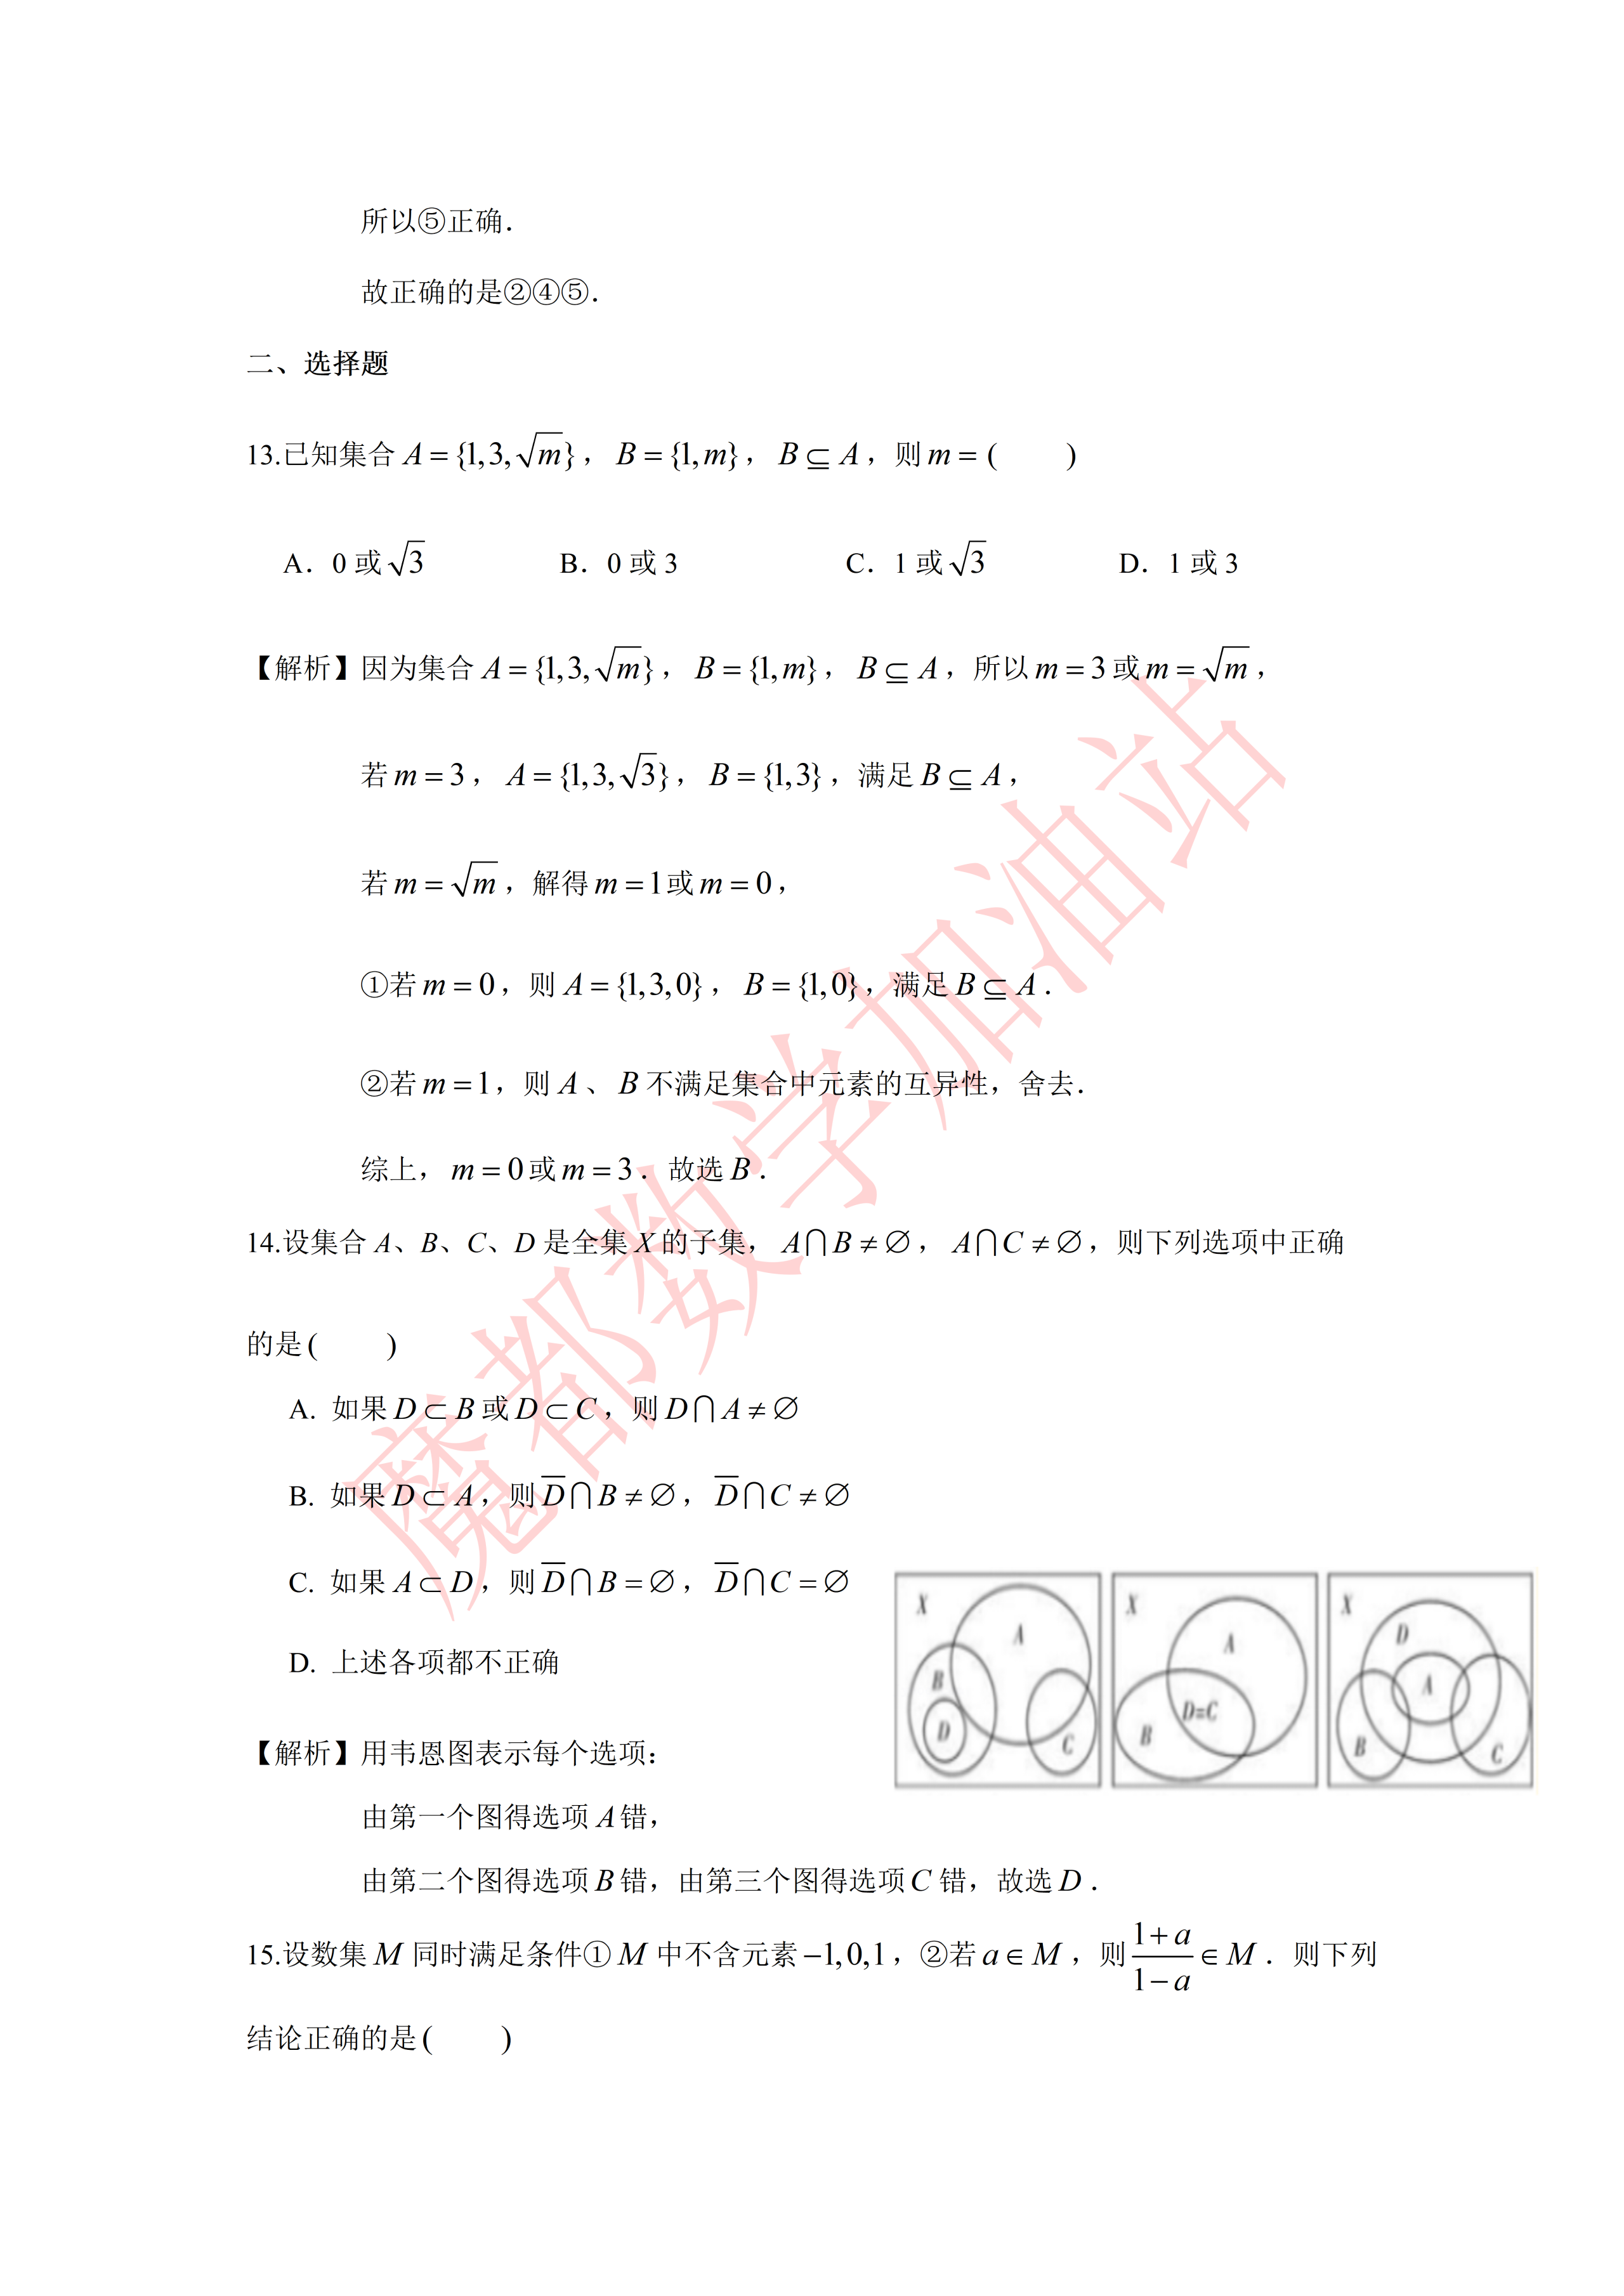
\includegraphics[width=.75\linewidth,trim=1400bp 790bp 135bp 1155bp,clip]{../原图/高一49_华师大二附中_国庆作业1/05.png}
\end{center}
\step{由第一个图得选项 $A$ 错，}
\step{由第二个图得选项 $B$ 错，由第三个图得选项 $C$ 错，故选 $D$.}
\solend
\fi

\item 设数集 $M$ 同时满足条件①$M$ 中不含元素 $-1$、$0$、$1$，②若 $a\in M$，则 $\dfrac{1+a}{1-a}\in M$．则下列结论正确的是\mbox{（\quad）}

\keepwithprev
A. 集合 $M$ 中至多有 $2$ 个元素\qquad B. 集合 $M$ 中至多有 $3$ 个元素

C. 集合 $M$ 中有且仅有 $4$ 个元素\qquad D. 集合 $M$ 中有无穷多个元素

\ifanswer
\solbegin
\step{若集合只含有一个元素，则 $\dfrac{1+a}{1-a}=a$，即 $1+a=a-a^2$，即 $-a^2=1$，不成立.}
\step{当 $a=3$ 时，$\dfrac{1+3}{1-3}=-2\in M$，所以 $\dfrac{1-2}{1+2}=-\dfrac13\in M$，所以 $\dfrac{1-\frac13}{1+\frac13}=\dfrac12\in M$，}
\step{所以 $\dfrac{1+\frac12}{1-\frac12}=3$，开始重复了，所以 $M=\left\{3,-2,-\dfrac13,\dfrac12\right\}$；}
\step{当 $a=2$ 时，$\dfrac{1+2}{1-2}=-3\in M$，所以 $\dfrac{1-3}{1+3}=-\dfrac12\in M$，所以 $\dfrac{1-\frac12}{1+\frac12}=\dfrac13\in M$，}
\step{所以 $\dfrac{1+\frac13}{1-\frac13}=2$，开始重复了，所以 $M=\left\{2,-3,-\dfrac12,-\dfrac13\right\}$，}
\step{此时也只要四个元素；}
\step{当 $a=\dfrac34\in M$，则 $7\in M$，若 $7\in M$，则 $-\dfrac43\in M$，}
\step{若 $-\dfrac43\in M$，则 $-\dfrac17\in M$，若 $-\dfrac17\in M$，有 $\dfrac34\in M$，}
\step{由归纳推理得，集合 $M$ 中有且仅有 $4$ 个元素．故选 $C$.}
\solend
\fi

\item 已知集合 $M=\{x\mid x\in\N,0<x\leqslant15\}$，$A_1$、$A_2$、$A_3$ 满足：①$A_1\cup A_2\cup A_3=M$；②每个集合都恰有 $5$ 个元素．集合 $A_i$（$i=1,2,3$）中最大元素与最小元素之和称为 $A_i$ 的特征数，记为 $X_i$（$i=1,2,3$），则 $X_1+X_2+X_3$ 的值不可能为\mbox{（\quad）}

\keepwithprev
A. $37$\qquad B. $39$\qquad C. $48$\qquad D. $57$

\ifanswer
\solbegin
\step{因为集合 $M=\{x\mid x\in\N,0<x\leqslant15\}=\{1,2,3,\cdots,15\}$，}
\step{又因为集合 $A_1$、$A_2$、$A_3$ 中，每个集合恰有 $5$ 个元素，}
\step{且 $A_1\cup A_2\cup A_3=M$ 有 $15$ 个元素，所以集合 $A_1$、$A_2$、$A_3$ 中没有重复元素，}
\step{因为 $1$ 是集合 $M$ 中数值最小的元素，$15$ 是集合 $M$ 中数值最大的元素，}
\step{所以在 $A_i$ 的特征数构成中，必有 $1$ 和 $15$，不妨设 $1\in A_1$，$15\in A_1$，}
\step{要使 $X_1+X_2+X_3$ 最大，则应该在集合 $A_1$ 中首先放置数值较小的元素，}
\step{即 $A_1=\{1,2,3,4,15\}$，所以 $5$ 与 $14$ 是剩下元素中数值最小或最大的元素，}
\step{同理，不妨设 $5\in A_2$，$14\in A_2$，接着在 $A_2$ 中再次放置数值较小的元素，}
\step{即 $A_2=\{5,6,7,8,14\}$，则 $A_3=\{9,10,11,12,13\}$，}
\step{此时 $X_1+X_2+X_3$ 有最大值为 $1+15+5+14+9+13=57$，}
\step{即 $X_1+X_2+X_3\leqslant57$；}
\step{要使 $X_1+X_2+X_3$ 最小，则在集合 $A_1$ 中首先放置数值较大的元素，}
\step{即 $A_1=\{1,12,13,14,15\}$，所以 $2$ 与 $11$ 是剩下元素中数值最小或最大的元素，}
\step{同理，不妨设 $2\in A_2$，$11\in A_2$，接着在 $A_2$ 中再次放置数值较大的元素，}
\step{即 $A_2=\{2,8,9,10,11\}$，则 $A_3=\{3,4,5,6,7\}$，}
\step{此时 $X_1+X_2+X_3$ 有最小值为 $1+15+2+11+3+7=39$，}
\step{即 $X_1+X_2+X_3\geqslant39$，}
\step{综上，$39\leqslant X_1+X_2+X_3\leqslant57$，故选 $A$.}
\solend
\fi

\end{enumerate}

\bigsec{三、解答题}

\begin{enumerate}
\setcounter{enumi}{16}

\item 已知全集为 $\R$，集合 $A=\{x\mid y=\sqrt{(2+x)(4-x)}\}$，$B=\{x\mid-1<x<m+1\}$.

\begin{enumerate}[label=(\arabic*)]
\item 若 $m=4$，求 $A\cup B$、$\overline A\cap B$；
\item 若 $B\subseteq A$，求实数 $m$ 的取值范围.
\end{enumerate}

\ifanswer
\solbegin
\stepm{(1)}{集合 $A=\{x\mid y=\sqrt{(2+x)(4-x)}\}=\{x\mid-2\leqslant x\leqslant4\}$，}
\step{当 $m=4$ 时，$B=\{x\mid-1<x<5\}$.}
\step{所以 $A\cup B=[-2,5)$，$\overline A=\{x\mid x<-2\text{ 或 }x>4\}$，$\overline A\cap B=(4,5)$.}
\stepm{(2)}{因为 $B\subseteq A$，}
% 原卷如此，照录未改（第 17 题(2)解析两处"当 C=∅／当 C≠∅"应为 B，本卷并无集合 C）
\step{当 $C=\varnothing$ 时，$m\leqslant-2$，$B\subseteq A$ 成立；}
\step{当 $C\neq\varnothing$ 时，$m>-2$，$-1<m+1\leqslant4$，解得 $-2<m\leqslant3$，}
\step{综上，$m\leqslant3$，所以实数 $m$ 的取值范围是 $(-\infty,3]$.}
\solend
\fi

\ansspace[6]

\item 用反证法证明：若 $a$、$b$、$c\in\R$，且 $x=a^2-2b+1$，$y=b^2-2c+1$，$z=c^2-2a+1$，则 $x$、$y$、$z$ 中至少有一个不小于 $0$.

\ifanswer
\solbegin
\step{假设 $x$、$y$、$z$ 均小于 $0$，即 $x=a^2-2b+1<0$①，$y=b^2-2c+1<0$②，}
\step{$z=c^2-2a+1<0$③，①$+$②$+$③得 $x+y+z=(a-1)^2+(b-1)^2+(c-1)^2<0$，}
\step{这与 $(a-1)^2+(b-1)^2+(c-1)^2\geqslant0$ 矛盾，则假设不成立，}
\step{所以 $x$、$y$、$z$ 中至少有一个不小于 $0$，得证.}
\solend
\fi

\ansspace[5]

\item 已知全集为 $\R$，实数 $a$、$b$ 满足 $a\neq b$，集合 $M=\{x\mid x^2-3x-4\leqslant0\}$，集合 $A=\{x\mid(x+a)(x+b)>0\}$，集合 $B=\{x\mid x^2+(a-2)x-2a>0\}$.

\begin{enumerate}[label=(\arabic*)]
\item 若 $\overline A=M$，求 $a$、$b$ 的值；
\item 若 $a>b>-1$，求 $A\cap B$；
\item 若 $a^2+a\in\overline B$，求 $a$ 的取值范围.
\end{enumerate}

\ifanswer
\solbegin
\stepm{(1)}{$M=\{x\mid x^2-3x-4\leqslant0\}=\{x\mid-1\leqslant x\leqslant4\}$，$A=\{x\mid(x+a)(x+b)\leqslant0\}$，}
\step{因为 $\overline A=M$，所以 $a=1$，$b=-4$ 或 $a=-4$，$b=1$.}
\stepm{(2)}{因为 $a>b>-1$，所以 $-a<-b<1$，所以 $A=\{x\mid x<-a\text{ 或 }x>-b\}$，}
\step{因为 $B=\{x\mid x^2+(a-2)x-2a>0\}=\{x\mid x<-a\text{ 或 }x>2\}$，}
\step{所以 $A\cap B=\{x\mid x<-a\text{ 或 }x>2\}$，}
\stepm{(3)}{$\overline B=\{x\mid(x-2)(x+a)\leqslant0\}$，}
% 原卷如此，照录未改（第 19 题(3)此处"a(a-1)((a-2)^2≤0"括号不配对；且由左式展开应为
% a(a-1)(a+2)^2≤0，与下句"解得 a=2 …[0,1]∪{2}"按 (a-2)^2 方自洽，见文件头清单第 2 条）
\step{由 $a^2+a\in\overline B$，得 $(a^2+a-2)(a^2+2a)\leqslant0\Leftrightarrow a(a-1)((a-2)^2\leqslant0$，}
\step{解得 $a=2$ 或 $0\leqslant a\leqslant1$，故 $a$ 的取值范围是 $[0,1]\cup\{2\}$.}
\solend
\fi

\ansspace[7]

\item 设数集 $A$ 由实数构成，若 $x\in A$（$x\neq1$ 且 $x\neq0$），则 $\dfrac{1}{1-x}\in A$.

\begin{enumerate}[label=(\arabic*)]
\item 若 $2\in A$，则 $A$ 中至少还有几个元素；
\item 集合 $A$ 是否为双元素集合？请说明理由；
\item 若 $A$ 中元素个数不超过 $8$ 个，所有元素的和为 $\dfrac{14}{3}$，且 $A$ 中有一个元素的平方等于所有元素的积，求集合 $A$.
\end{enumerate}

\ifanswer
\solbegin
\stepm{(1)}{若 $x\in A$，则 $\dfrac{1}{1-x}\in A$，又 $2\in A$，所以 $\dfrac{1}{1-2}=-1\in A$，}
\step{所以 $\dfrac{1}{1-(-1)}=\dfrac12\in A$，所以 $\dfrac{1}{1-\frac12}=2\in A$，}
% 原卷如此，照录未改（第 20 题(1)解析末句"2 个几个元素"衍一"几个"）
\step{所以 $A$ 中至少还有 $2$ 个几个元素；}
\stepm{(2)}{若 $x\in A$（$x\neq1$ 且 $x\neq0$），则 $\dfrac{1}{1-x}\in A$，}
\step{则 $\dfrac{1}{1-\frac{1}{1-x}}=\dfrac{1-x}{-x}\in A$，则 $\dfrac{1}{1-\frac{1-x}{-x}}=x\in A$}
\step{若 $A$ 为双元素集，则 $x=\dfrac{1}{1-x}$ 或 $x=\dfrac{1-x}{-x}$ 或 $\dfrac{1}{1-x}=\dfrac{1-x}{-x}$，均无解，}
\step{所以 $A$ 不可能为双元素集；}
\stepm{(3)}{由 $x\in A$，$\dfrac{1}{1-x}\in A$，得 $\dfrac{1}{1-\frac{1}{1-x}}=\dfrac{x-1}{x}\in A$，得 $\dfrac{1}{1-\frac{x-1}{x}}=x\in A$，}
\step{所以 $\left\{x,\dfrac{1}{1-x},\dfrac{x-1}{x}\right\}\subseteq A$，而 $x\cdot\dfrac{1}{1-x}\cdot\dfrac{x-1}{x}=-1$，}
\step{$A$ 中元素个数为 $3$ 的倍数，则 $A$ 中元素只有 $6$ 个，}
\step{因为 $A$ 中有一个元素的平方等于所有元素的积，}
\step{不妨设 $x^2=1$，解得 $x=-1$ 或 $x=1$（舍），则 $-1$、$\dfrac12$、$2\in A$，}
\step{所以 $-1+\dfrac12+2+m+\dfrac{1}{1-m}+\dfrac{m-1}{m}=\dfrac{14}{3}$，解得 $m=-\dfrac12$ 或 $m=3$ 或 $m=\dfrac23$，}
\step{所以 $A=\left\{\dfrac12,2,-1,-\dfrac12,3,\dfrac23\right\}$.}
\solend
\fi

\ansspace[9]

% 原卷如此，照录未改（第 21 题题干"21.求已知集合"之"求"字疑衍；"任意两个元素 a_i a_j"
% 疑脱逗号；"|a_i-a_j|≥1/30 则称"之前疑脱标点，见文件头清单第 4 条）
\item 求已知集合 $M=\left\{\dfrac{1}{k}\middle|1\leqslant k\leqslant100\text{ 且 }k\in\N^{*}\right\}$，$A=\{a_1,a_2,\cdots,a_n\}$，其中 $n\in\N^{*}$，且 $n\geqslant2$．若 $A\subseteq\N$，且对集合 $A$ 中的任意两个元素 $a_ia_j$，$i\neq j$ 都有 $|a_i-a_j|\geqslant\dfrac{1}{30}$ 则称集合 $A$ 有性质 $P$.

\begin{enumerate}[label=(\arabic*)]
\item 判断集合 $\left\{\dfrac13,\dfrac14,\dfrac15,\dfrac16,\dfrac17\right\}$ 是否具有性质 $P$；
\item 若集合 $A=\{a_1,a_2,\cdots,a_n\}$ 具有性质 $P$.

①求证：$a_i-a_j$ 的最大值大于等于 $\dfrac{n-1}{30}$；

②求 $A$ 的元素个数 $n$ 的最大值.
\end{enumerate}

\ifanswer
\solbegin
\stepm{(1)}{集合为 $\left\{\dfrac13,\dfrac14,\dfrac15,\dfrac16,\dfrac17\right\}$，又 $\dfrac16-\dfrac17=\dfrac{1}{42}<\dfrac{1}{30}$，所以该集合不具有性质 $P$；}
\stepm{(2)}{①因为集合 $A=\{a_1,a_2,\cdots,a_n\}$ 具有性质 $P$，}
\step{不妨设 $a_1<a_2<a_3<\cdots<a_n$，则 $a_i-a_j\geqslant\dfrac{1}{30}$（$i>j$），}
\step{所以 $a_n-a_1=(a_n-a_{n-1})+(a_{n-1}-a_{n-2})+\cdots+(a_2-a_1)\geqslant\dfrac{n-1}{30}$，}
\step{故 $a_i-a_j$ 的最大值大于等于 $\dfrac{n-1}{30}$；}
% 原卷如此，照录未改（第 21 题(2)②首行"a_2-a_1≥(n-1)/30"：由①同款推理只能得
% a_2-a_1≥1/30，见文件头清单第 5 条）
\step{②$A=\{a_1,a_2,\cdots,a_n\}$，不妨设 $a_1<a_2<a_3<\cdots<a_n$，}
\step{要使 $A$ 的元素个数 $n$ 最大，}
\step{则 $A$ 中的元素满足 $a_n=\dfrac{1}{k}$，$a_{n-1}=\dfrac{1}{k+1}$，$\cdots$，$a_1=\dfrac{1}{k+n-1}$（$k\in\N^{*}$），}
\step{又由①得 $a_2-a_1=\dfrac{1}{k+n-2}-\dfrac{1}{k+n-1}\geqslant\dfrac{n-1}{30}$，}
\step{所以 $(k+n-2)(k+n-1)\leqslant30$，又 $a_n-a_{n-1}=\dfrac{1}{k}-\dfrac{1}{k+1}\geqslant\dfrac{1}{30}$，}
\step{所以 $k(k+1)\leqslant30$，所以 $1\leqslant k\leqslant5$（$k\in\N^{*}$），}
\step{当 $k=5$ 时，由 $(k+n-2)(k+n-1)\leqslant30$，解得 $n\leqslant2$，$n\in\N^{*}$；}
\step{当 $k=4$ 时，由 $(k+n-2)(k+n-1)\leqslant30$，解得 $n\leqslant3$，$n\in\N^{*}$；}
\step{当 $k=3$ 时，由 $(k+n-2)(k+n-1)\leqslant30$，解得 $n\leqslant4$，$n\in\N^{*}$；}
\step{当 $k=2$ 时，由 $(k+n-2)(k+n-1)\leqslant30$，解得 $n\leqslant5$，$n\in\N^{*}$；}
\step{当 $k=1$ 时，由 $(k+n-2)(k+n-1)\leqslant30$，解得 $n\leqslant6$，$n\in\N^{*}$.}
\step{故 $A$ 的元素个数 $n$ 的最大值为 $6$，此时集合 $A=\left\{1,\dfrac12,\dfrac13,\cdots,\dfrac16\right\}$.}
\solend
\fi

\ansspace*[10]

\end{enumerate}

\end{document}
"
%
% 原始材料：微信公众号"魔都数学加油站"文章，作者破晓，连载"27学年高一49"；
% 原文标题"27学年高一49——2026-2027年上海市华师大二附中高一上国庆作业1集合与逻辑、
% 等式与不等式的性质"；页面用 JS 渲染，未见明确发布日期（页内时间戳 ≈ 2026-10-05 21:37）；
% 原文链接：https://mp.weixin.qq.com/s/XxZTOBVQslK5cZm2_BbhOg。
% 正文为 11 张 PNG 页：第 01、03、04、06、07、08、09 页 4762×6735，
% 第 02、05、10、11 页 2560×3620，均按页序读取；粉色斜排"魔都数学加油站"为卷面水印，
% 与公众号页脚一并未录入。全卷 11 页均为试卷页，无二维码/宣传页。
%
% 题号与分节：原文自第 3 题起编，填空题 3—12、选择题 13—16、解答题 17—21，共 19 题。
% 讲评版：原卷每题下直接印【答案】或【解析】——只印【答案】的 3 题（第 3、5、8 题），
% 其余 16 题均只印【解析】；解析行数已逐题按印刷行照录（一条 \step＝原卷一个印刷行）。
%
% 卷首标题：照卷面印作"2026-2027 年华师大二附中高一上国庆作业 1"（公众号标题中的"上海市"
% 卷面没有，本稿照卷面），年份区间按全稿惯例排 en dash；副标题照卷面自印的
% "集合与逻辑单元综合检测"（原卷页首标题行下方即印此行，故不另按模块口径拟名）。
% 副标题依据：全卷 19 题均为集合与常用逻辑用语内容——集合类 15 题（6—17、19—21 中除
% 反证法题外），逻辑/命题类 3 题（第 3 题否定形式、第 4 题充要条件、第 5 题反证法假设），
% 反证法证明 1 题（第 18 题）；全卷无不等式求解题，公众号标题中"等式与不等式的性质"
% 与卷面实际内容不符。
%
% 与原卷的排版差异：
%   ① 原文从第 3 题起，填空题为 3—12、选择题为 13—16、解答题为 17—21，本稿保留原题号；
%   ② 原卷每题下直接印【答案】/【解析】，本稿按全稿惯例置于答案版；只印【解析】的题
%      不另提 \ans{}（照 高一36 口径），只印【答案】的题仅给 \ans{}；
%   ③ 原卷第 8 题韦恩图排在题干右侧、第 14 题三联韦恩图排在选项（C、D）右侧，
%      本稿分别移至题干下方、解析首步之后居中排，均直接裁取原图页（02.png、05.png）；
%   ④ 数集记号原卷排作斜体/加粗 R、N、Z，本稿统一为 \R、\N、\Z、\N^*；
%      填空横线按全稿惯例排为 \blankline[4.4em]。
%
% 原卷笔误/存疑清单（均照录未改，正文中该处有 % 注）：
%   1. 第 17 题(2)解析两处"当 C=∅／当 C≠∅"应为 B（本卷并无集合 C）；
%   2. 第 19 题(3)解析"a(a-1)((a-2)^2≤0"括号不配对（多一枚左括号）；且由
%      (a^2+a-2)(a^2+2a)≤0 展开应为 a(a-1)(a+2)^2≤0，与原卷结论"解得 a=2 …
%      [0,1]∪{2}"恰按 (a-2)^2 自洽——因式分解与原式不符，结论按 (a-2)^2 自洽，均照录；
%   3. 第 20 题(1)解析末句"至少还有 2 个几个元素"衍一"几个"；
%   4. 第 21 题题干"21.求已知集合"之"求"字疑衍；"任意两个元素 a_i a_j"疑脱逗号；
%      "≥1/30 则称"之前疑脱标点；
%   5. 第 21 题(2)②解析"a_2-a_1≥(n-1)/30"：由①同款推理只能得 a_2-a_1≥1/30，
%      原卷如此，照录未改（后续 (k+n-2)(k+n-1)≤30 即按该行推得）。
%
\documentclass[a4paper,11pt]{article}
\usepackage{common}

\begin{document}

\examtitlest[3]{2026--2027 年华师大二附中高一上国庆作业 1}{集合与逻辑单元综合检测}

\bigsec{一、填空题}

\begin{enumerate}
\setcounter{enumi}{2}

\item “若 $x^2-x-2\leqslant0$，则 $-1\leqslant x\leqslant2$”的否定形式为\blankline[4.4em].

\ifanswer
\ans{若 $x^2-x-2>0$，则 $x<-1$ 或 $x>2$}
\fi

\item 已知 $p:|x-3|<5$，$q:1-a<x<2a-3$，且 $p$ 是 $q$ 的充分非必要条件，则实数 $a$ 的取值范围是\blankline[4.4em].

\ifanswer
\solbegin
\step{由 $|x-3|<5$ 得 $-2<x<8$，}
\step{又 $p$ 是 $q$ 的充分不必要条件，所以 $(-2,8)\subset(1-a,2a-3)$，}
\step{即 $\begin{cases}-2\geqslant1-a\\ 8\leqslant2a-3\\ (2a-3)-(1-a)\neq8-(-2)\end{cases}$，解得 $a\geqslant\dfrac{11}{2}$，实数 $a$ 的取值范围是 $\left[\dfrac{11}{2},+\infty\right)$.}
\solend
\fi

\item 用反证法证明命题“设 $a$、$b\in\R$，则方程 $a_1x^2+b_1x+c_1=0$ 与 $a_2x^2+b_2x+c_2=0$ 至少有一个实根”时要做的假设是\blankline[4.4em].

\ifanswer
\ans{假设 $a$、$b\in\R$，方程 $a_1x^2+b_1x+c_1=0$ 与 $a_2x^2+b_2x+c_2=0$ 都没有实根}
\fi

\item 设集合 $A=\{x\mid x^2-mx+6=0,x\in\R\}$，且 $A\cap\{2,3\}=A$，则实数 $m$ 的取值范围是\blankline[4.4em].

\ifanswer
\solbegin
\step{由 $A\cap\{2,3\}=A$，得 $A\subseteq\{2,3\}$，}
\step{当 $A=\varnothing$ 时，$\Delta=m^2-24<0$，解得 $-2\sqrt6<m<2\sqrt6$；}
\step{当 $A=\{2\}$ 时，$\begin{cases}2^2-2m+6=0\\ \Delta=m^2-24=0\end{cases}$，无解；}
\step{当 $A=\{3\}$ 时，$\begin{cases}3^2-3m+6=0\\ \Delta=m^2-24=0\end{cases}$，无解；}
\step{当 $A=\{2,3\}$ 时，$\begin{cases}3^2-3m+6=0\\ 2^2-2m+6=0\end{cases}$，解得 $m=5$，}
\step{所以实数 $m$ 的取值范围是 $(-2\sqrt6,2\sqrt6)\cup\{5\}$.}
\solend
\fi

\item 已知 $a\in\R$，集合 $A=\left\{x\middle|\dfrac12a-1<x<\dfrac12a+1\right\}$，设关于 $x$ 的不等式 $ax<a^2+x-1$ 的解集为 $B$，若 $A\subset B$，则实数 $a$ 的取值范围为\blankline[4.4em].

\ifanswer
\solbegin
\step{因为 $ax<a^2+x-1$，所以 $(a-1)x<(a-1)(a+1)$，}
\step{①当 $a=1$ 时，$B=\varnothing$，$A\subset B$ 不可能成立；}
\step{②当 $a<1$ 时，$B=\{x\mid x>a+1\}$，因为 $A\subset B$，所以 $\dfrac12a-1\geqslant a+1$，}
\step{即 $a\leqslant-4$；}
\step{③当 $a>1$ 时，$B=\{x\mid x<a+1\}$，因为 $A\subset B$，所以 $\dfrac12a+1\leqslant a+1$，}
\step{即 $a>1$；}
\step{综上所述，实数 $a$ 的取值范围为 $(-\infty,-4]\cup(1,+\infty)$.}
\solend
\fi

\needvspace{8\baselineskip}

\item 已知 $U$ 为全集，$M$、$P$、$S$ 是 $U$ 的三个子集，用交、并、补关系将图中的阴影部分表示出来\blankline[4.4em].

\begin{center}
% 原图第 2 页题旁韦恩图直接裁取（原卷排于题干右侧）。
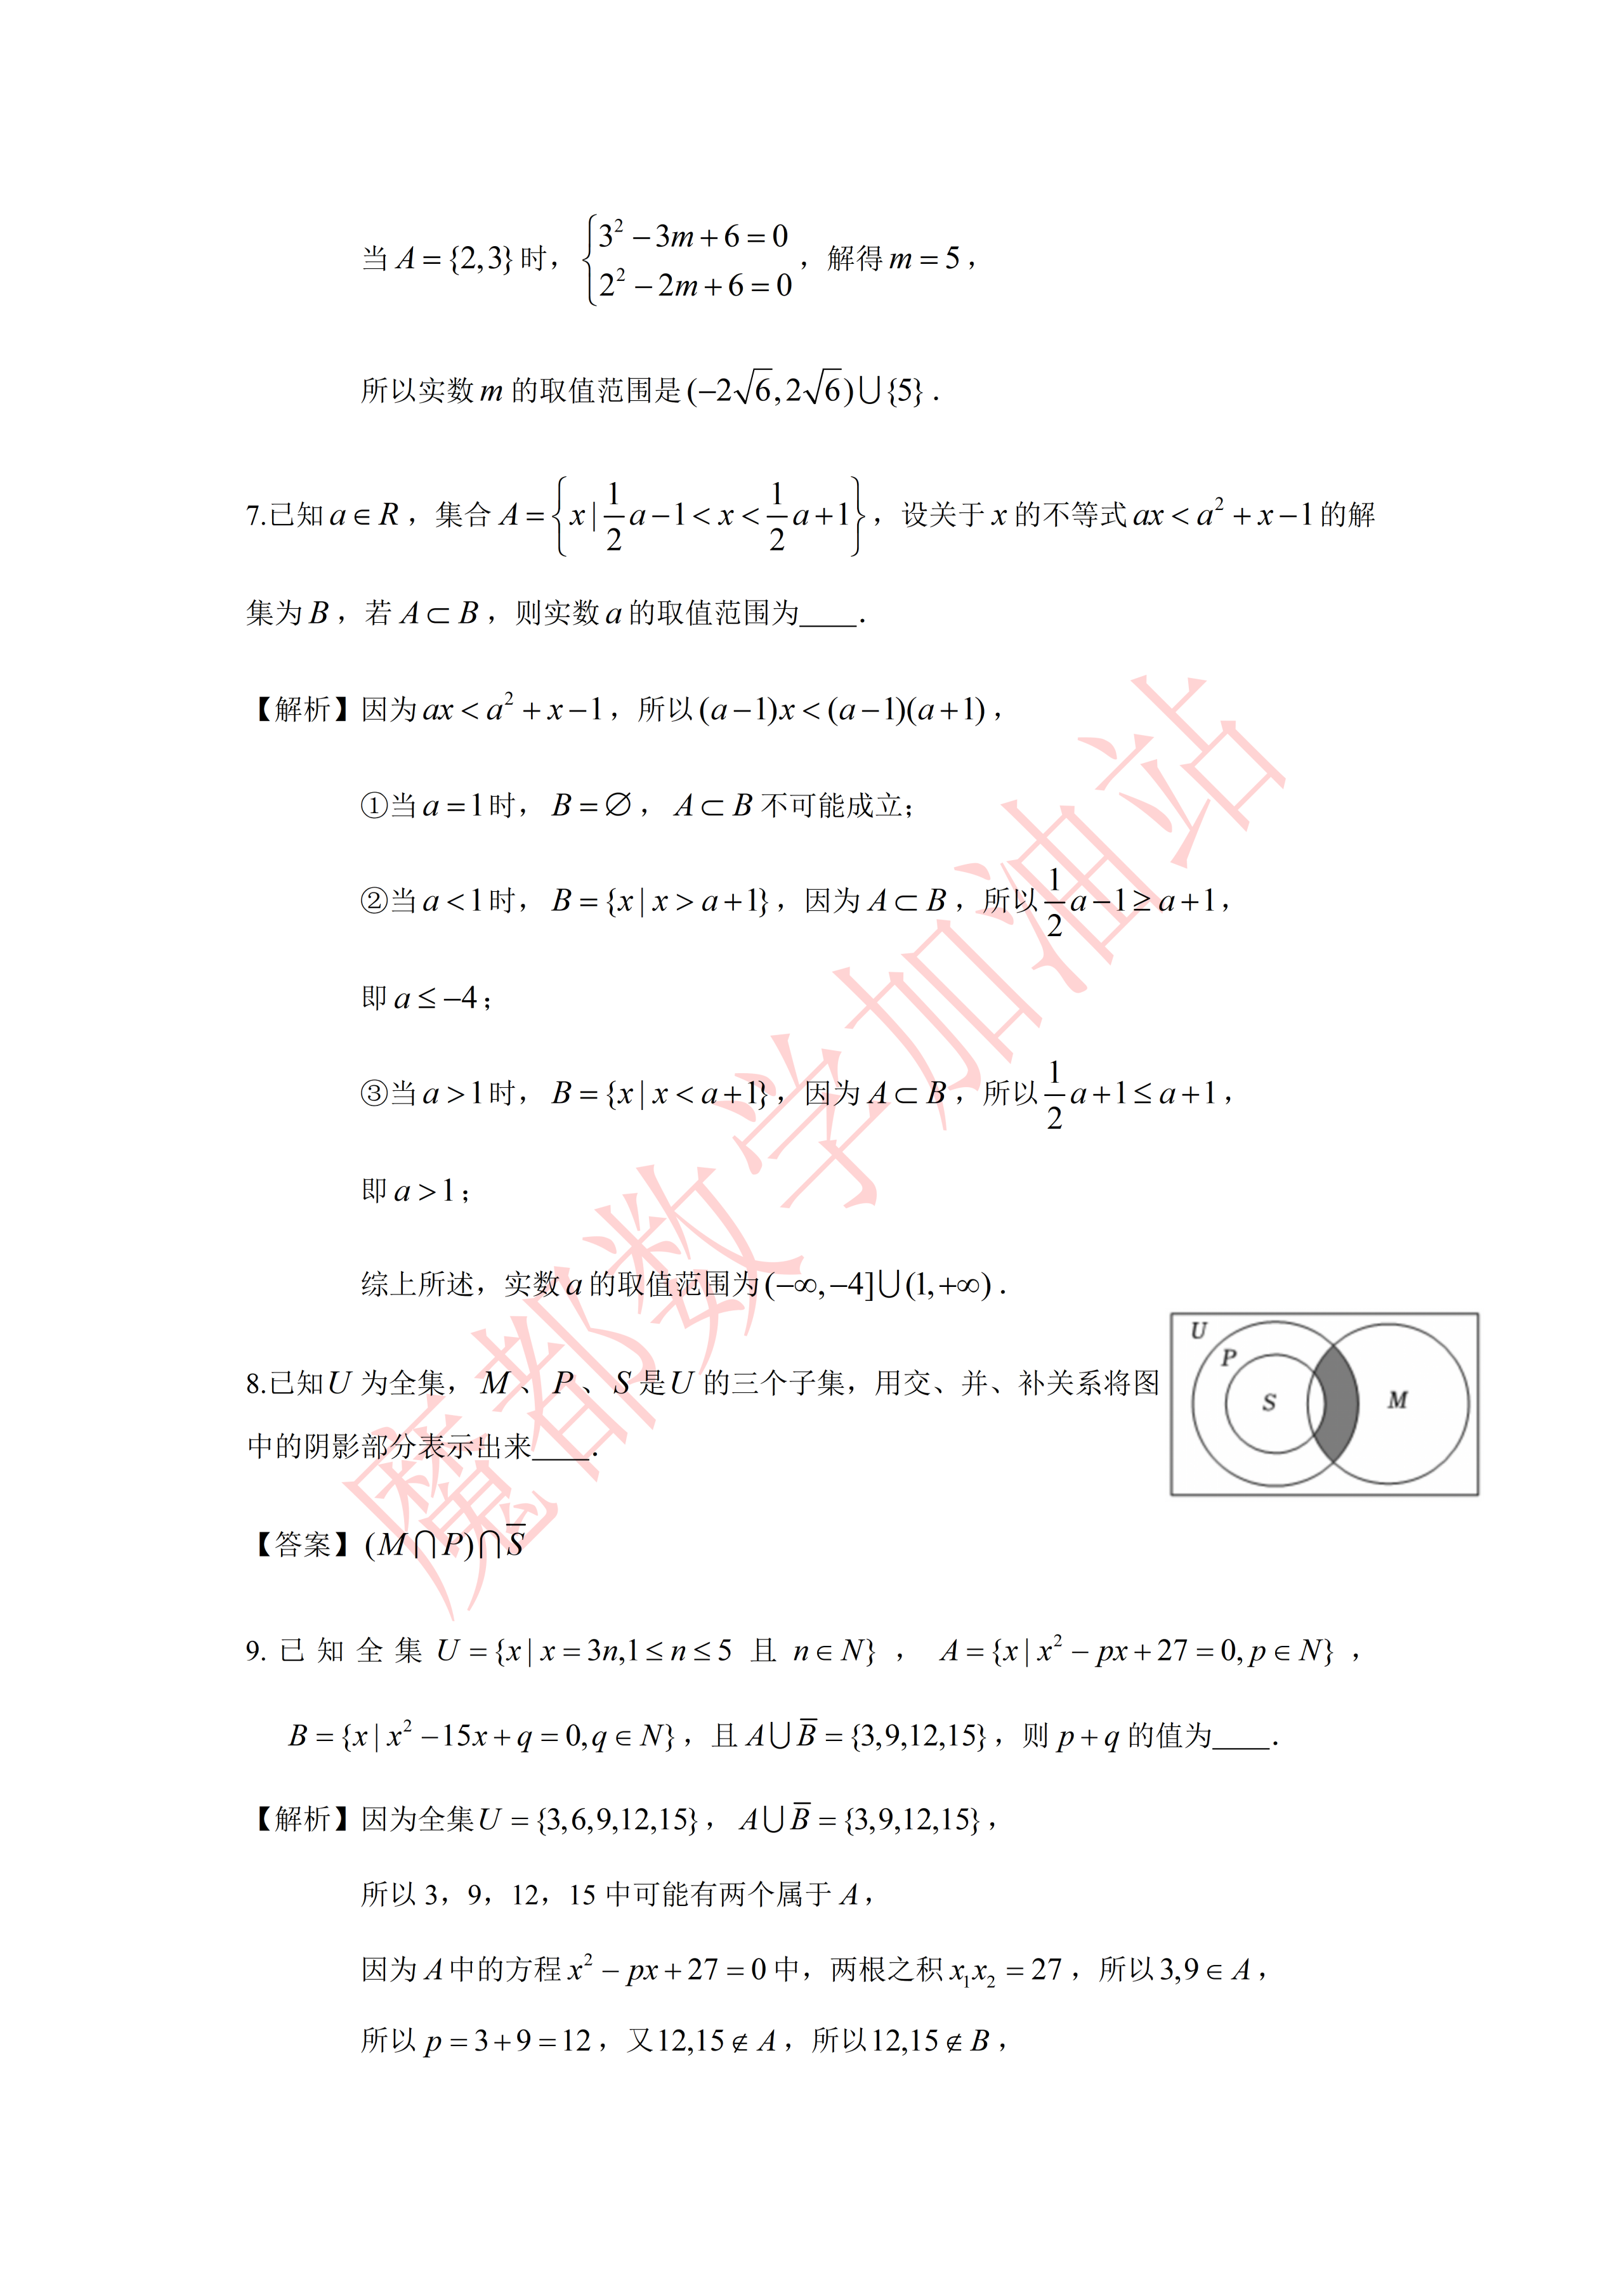
\includegraphics[width=.38\linewidth,trim=1835bp 1255bp 220bp 1565bp,clip]{../原图/高一49_华师大二附中_国庆作业1/02.png}
\end{center}

\ifanswer
\ans{$(M\cap P)\cap\overline S$}
\fi

\item 已知全集 $U=\{x\mid x=3n,1\leqslant n\leqslant5\text{ 且 }n\in\N\}$，$A=\{x\mid x^2-px+27=0,p\in\N\}$，$B=\{x\mid x^2-15x+q=0,q\in\N\}$，且 $A\cup\overline B=\{3,9,12,15\}$，则 $p+q$ 的值为\blankline[4.4em].

\ifanswer
\solbegin
\step{因为全集 $U=\{3,6,9,12,15\}$，$A\cup\overline B=\{3,9,12,15\}$，}
\step{所以 $3$、$9$、$12$、$15$ 中可能有两个属于 $A$，}
\step{因为 $A$ 中的方程 $x^2-px+27=0$ 中，两根之积 $x_1x_2=27$，所以 $3,9\in A$，}
\step{所以 $p=3+9=12$，又 $12,15\notin A$，所以 $12,15\notin B$，}
\step{因为 $B$ 中的方程 $x^2-15x+q=0$ 中，两根之和 $x_3+x_4=15$，所以 $6,9\in B$，}
\step{则 $q=6\times9=54$，所以 $p+q=66$.}
\solend
\fi

\item 已知集合 $A=\{x\mid x^2+(2a-3)x-3a=0,a\in\R,x\in\R\}$，集合 $B=\{x\mid x^2+(a-3)x+a^2-3a=0,a\in\R,x\in\R\}$，若 $A\neq B$，$A\cap B\neq\varnothing$，则 $A\cup B=$\blankline[4.4em].

\ifanswer
\solbegin
\step{设两个集合中的方程的公共解是 $b$，}
\step{由 $b^2+(2a-3)b-3a=b^2+(a-3)b+a^2-3a$，得 $ab=a^2$，}
\step{则 $a=0$ 或 $b=a$，}
\step{当 $a=0$ 时，不合题意，}
\step{当 $b=a$ 时，即两个方程的公共解为 $b=a$，}
\step{将 $b=a$ 代入方程，得 $a^2=2a$，$a=2$，}
\step{所以 $A=\{2,-3\}$，$B=\{-1,2\}$，所以 $A\cup B=\{-1,2,-3\}$.}
\solend
\fi

\item 已知一个有四个数字元素的集合 $S$，$S$ 的所有子集的元素和（空集的元素和认为是 $0$）的总和为 $16192$，则 $S$ 的元素之和等于\blankline[4.4em].

\ifanswer
\solbegin
\step{设 $S=\{a_1,a_2,a_3,a_4\}$，$S$ 的每个元素在所有子集中均出现 $2^3$ 次，}
\step{故 $(a_1+a_2+a_3+a_4)\cdot2^3=16192$，所以 $a_1+a_2+a_3+a_4=2024$，}
\step{故 $S$ 的元素之和等于 $2024$.}
\solend
\fi

\item 设 $P$ 为非空实数集满足：对任意给定的 $x,y\in P$（$x$、$y$ 可以相同），都有 $x+y\in P,x-y\in P,xy\in P$，则称 $P$ 为封闭集．关于封闭集有下列结论：

①集合 $P=\{-2,-1,0,1,2\}$ 为封闭集；

②集合 $P=\{x\mid x=2n,n\in\Z\}$ 为封闭集；

③若集合 $P_1$、$P_2$ 为封闭集，则 $P_1\cup P_2$ 为封闭集；

④若集合 $P$ 为封闭集，则一定有 $0\in P$；

⑤若集合 $P_1$、$P_2$ 为封闭集，则 $P_1\cap P_2$ 为封闭集.

其中正确结论的序号是\blankline[4.4em].

\ifanswer
\solbegin
\step{对于集合 $P=\{-2,-1,0,1,2\}$，取 $x=2$，$y=-2$，则 $x-y=2-(-2)=4\notin P$，}
\step{不满足封闭集的定义，所以①错误.}
\step{对于集合 $P=\{x\mid x=2n,n\in\Z\}$，设 $x=2n_1$，$y=2n_2$，$n_1,n_2\in\Z$.}
\step{$x+y=2n_1+2n_2=2(n_1+n_2)$，因为 $n_1+n_2\in\Z$，所以 $x+y\in P$.}
\step{$x-y=2n_1-2n_2=2(n_1-n_2)$，因为 $n_1-n_2\in\Z$，所以 $x-y\in P$.}
\step{$xy=2n_1\times2n_2=4n_1n_2=2(2n_1n_2)$，因为 $2n_1n_2\in\Z$，所以 $xy\in P$.}
\step{满足封闭集的定义，所以②正确.}
\step{令 $P_1=\{x\mid x=2n,n\in\Z\}$，$P_2=\{x\mid x=3n,n\in\Z\}$，都是封闭集.}
\step{$P_1\cup P_2$ 中，取 $x=2(x\in P_1)$，$y=3(y\in P_2)$，$x+y=5\notin P_1\cup P_2$，}
\step{不满足封闭集的定义，所以③错误.}
\step{因为对任意 $x\in P$，有 $x-x=0\in P$，}
\step{所以若集合 $P$ 为封闭集，则一定有 $0\in P$，所以④正确.}
\step{因为 $P_1$、$P_2$ 为封闭集，设 $x,y\in P_1\cap P_2$，则 $x,y\in P_1$ 且 $x,y\in P_2$.}
\step{因为 $P_1$ 是封闭集，所以 $x+y\in P_1,x-y\in P_1,xy\in P_1$.}
\step{因为 $P_2$ 是封闭集，所以 $x+y\in P_2,x-y\in P_2,xy\in P_2$.}
\step{所以 $x+y\in P_1\cap P_2,x-y\in P_1\cap P_2,xy\in P_1\cap P_2$，满足封闭集的定义，}
\step{所以⑤正确.}
\step{故正确的是②④⑤.}
\solend
\fi

\end{enumerate}

\bigsec{二、选择题}

\begin{enumerate}
\setcounter{enumi}{12}

\item 已知集合 $A=\{1,3,\sqrt m\}$，$B=\{1,m\}$，$B\subseteq A$，则 $m=$\mbox{（\quad）}

\keepwithprev
A. $0$ 或 $\sqrt3$\qquad B. $0$ 或 $3$

C. $1$ 或 $\sqrt3$\qquad D. $1$ 或 $3$

\ifanswer
\solbegin
\step{因为集合 $A=\{1,3,\sqrt m\}$，$B=\{1,m\}$，$B\subseteq A$，所以 $m=3$ 或 $m=\sqrt m$，}
\step{若 $m=3$，$A=\{1,3,\sqrt3\}$，$B=\{1,3\}$，满足 $B\subseteq A$，}
\step{若 $m=\sqrt m$，解得 $m=1$ 或 $m=0$，}
\step{①若 $m=0$，则 $A=\{1,3,0\}$，$B=\{1,0\}$，满足 $B\subseteq A$.}
\step{②若 $m=1$，则 $A$、$B$ 不满足集合中元素的互异性，舍去.}
\step{综上，$m=0$ 或 $m=3$．故选 $B$.}
\solend
\fi

\needvspace{10\baselineskip}

\item 设集合 $A$、$B$、$C$、$D$ 是全集 $X$ 的子集，$A\cap B\neq\varnothing$，$A\cap C\neq\varnothing$，则下列选项中正确的是\mbox{（\quad）}

\keepwithprev
A. 如果 $D\subset B$ 或 $D\subset C$，则 $D\cap A\neq\varnothing$

B. 如果 $D\subset A$，则 $\overline D\cap B\neq\varnothing$，$\overline D\cap C\neq\varnothing$

C. 如果 $A\subset D$，则 $\overline D\cap B=\varnothing$，$\overline D\cap C=\varnothing$

D. 上述各项都不正确

\ifanswer
\solbegin
\step{用韦恩图表示每个选项：}
\begin{center}
% 原图第 5 页解析配图（三联韦恩图）直接裁取（原卷排于选项 C、D 右侧）。
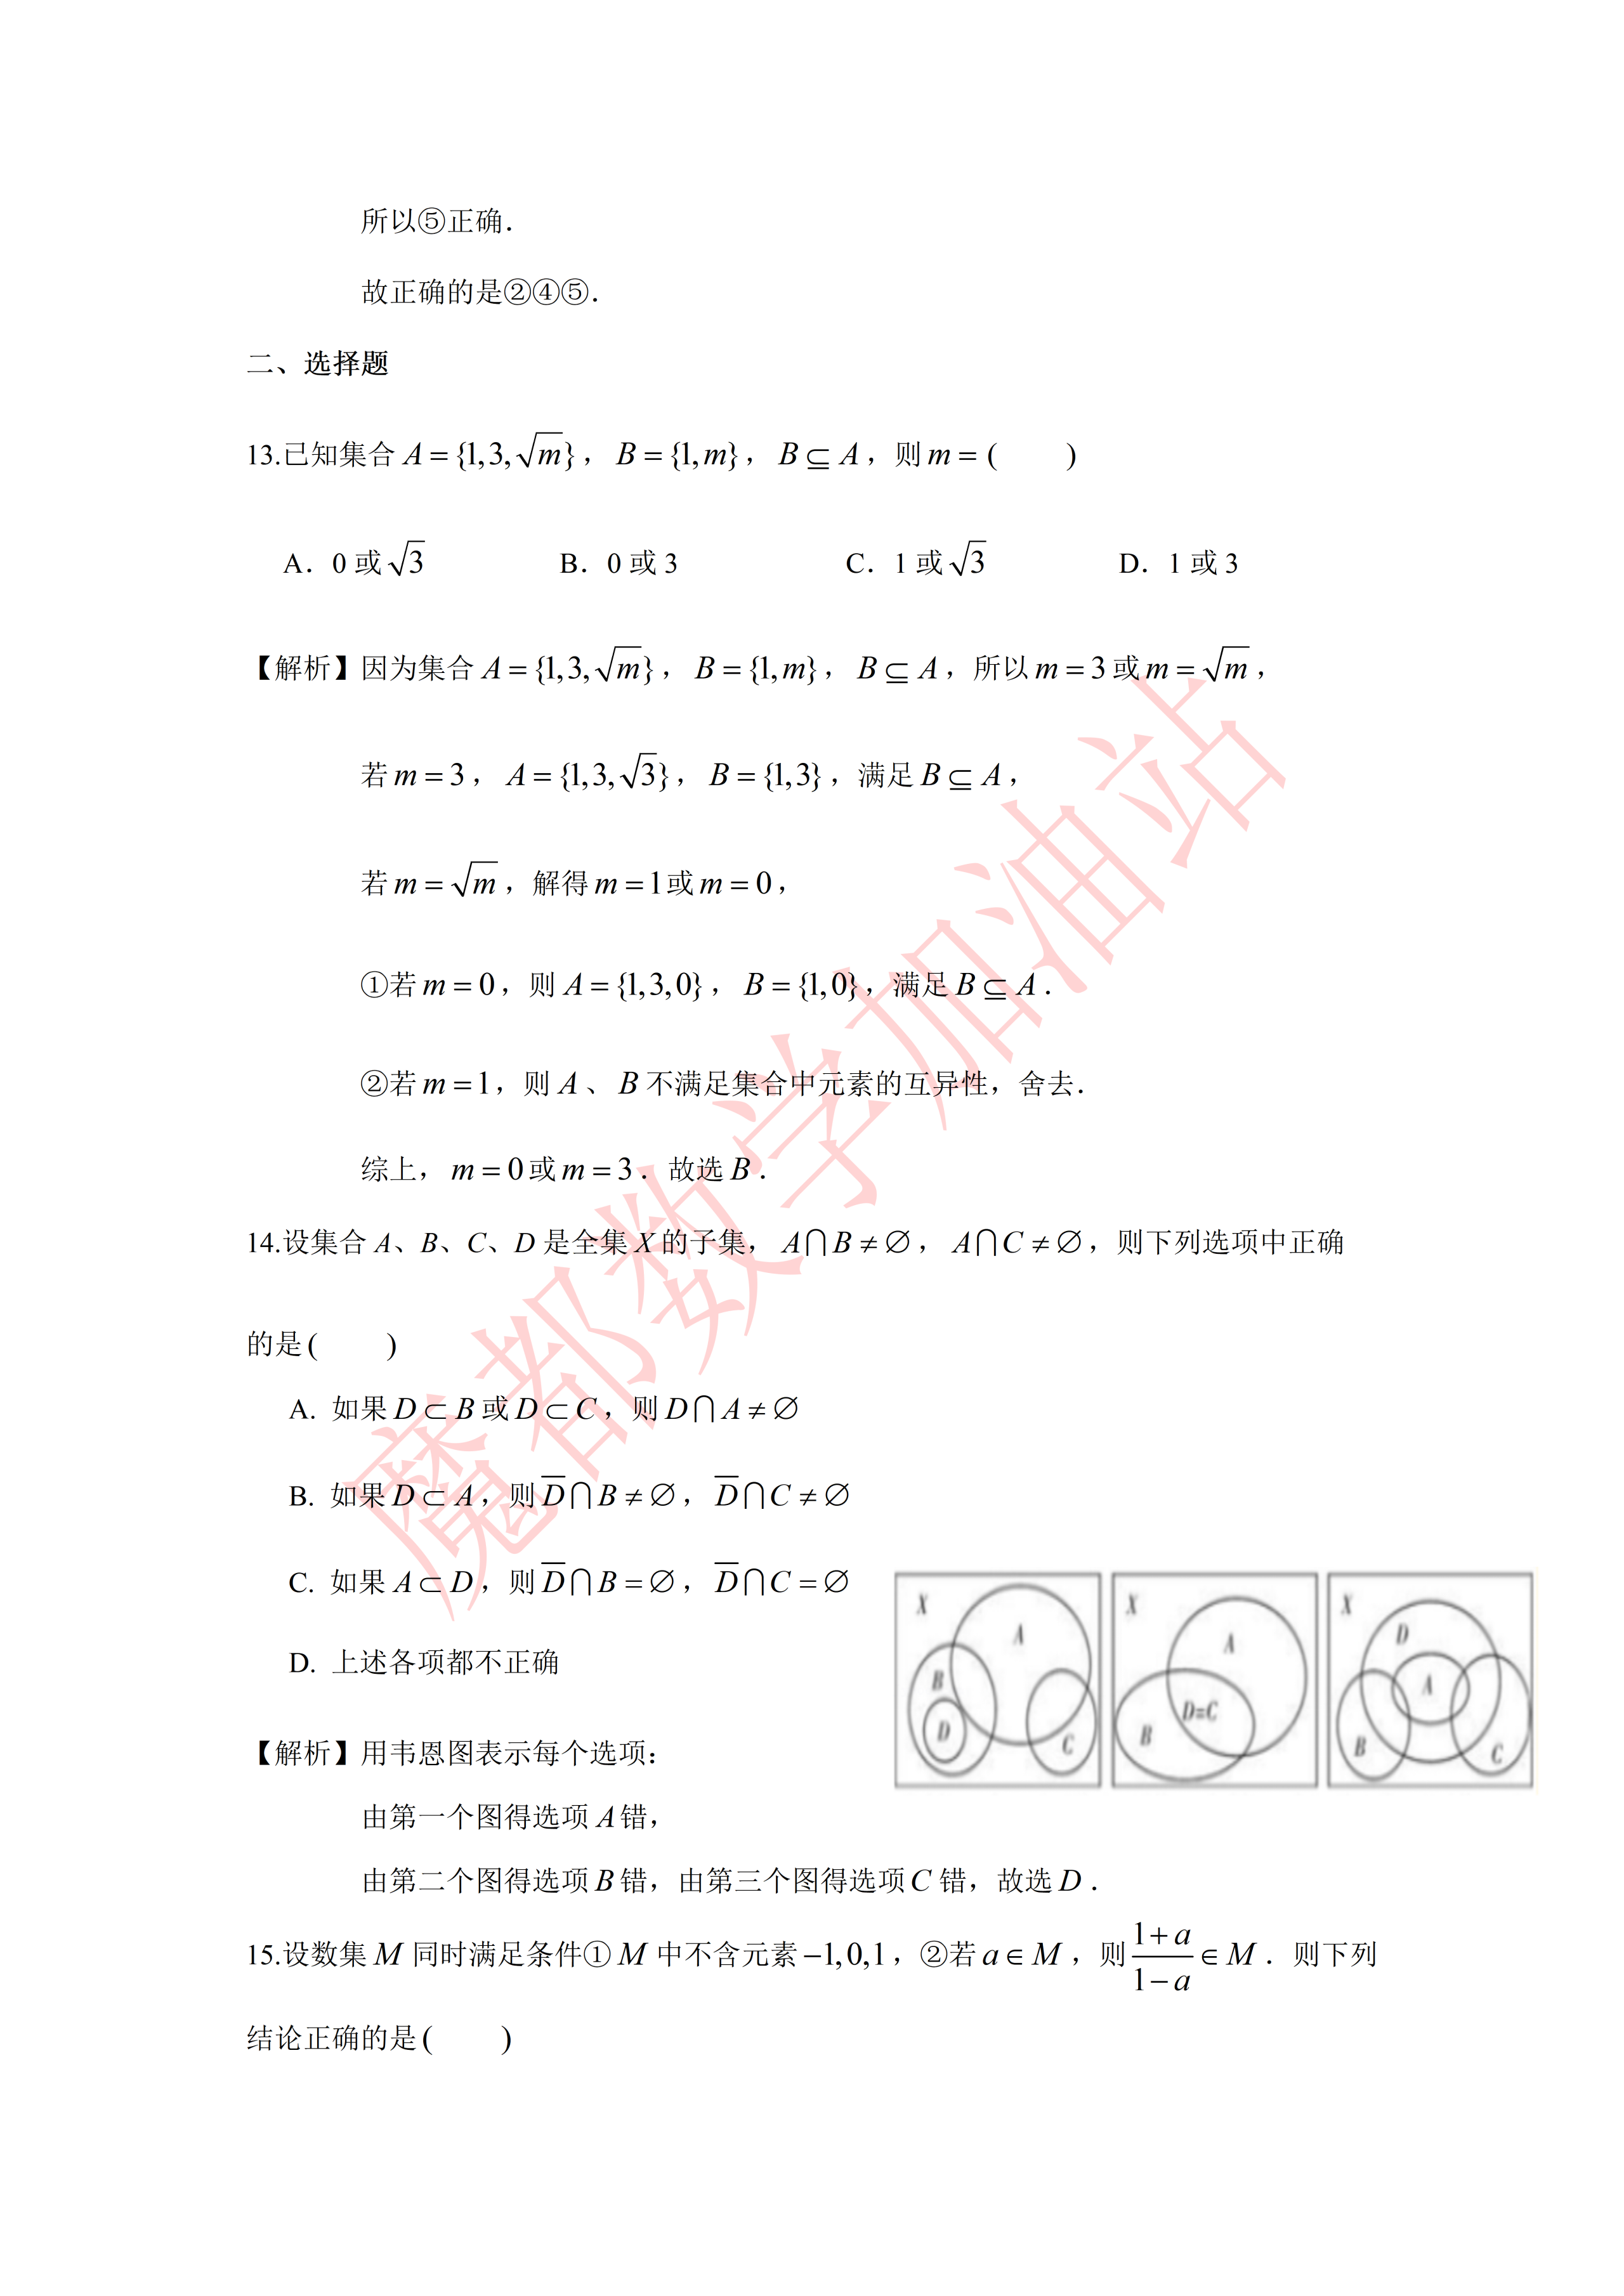
\includegraphics[width=.75\linewidth,trim=1400bp 790bp 135bp 1155bp,clip]{../原图/高一49_华师大二附中_国庆作业1/05.png}
\end{center}
\step{由第一个图得选项 $A$ 错，}
\step{由第二个图得选项 $B$ 错，由第三个图得选项 $C$ 错，故选 $D$.}
\solend
\fi

\item 设数集 $M$ 同时满足条件①$M$ 中不含元素 $-1$、$0$、$1$，②若 $a\in M$，则 $\dfrac{1+a}{1-a}\in M$．则下列结论正确的是\mbox{（\quad）}

\keepwithprev
A. 集合 $M$ 中至多有 $2$ 个元素\qquad B. 集合 $M$ 中至多有 $3$ 个元素

C. 集合 $M$ 中有且仅有 $4$ 个元素\qquad D. 集合 $M$ 中有无穷多个元素

\ifanswer
\solbegin
\step{若集合只含有一个元素，则 $\dfrac{1+a}{1-a}=a$，即 $1+a=a-a^2$，即 $-a^2=1$，不成立.}
\step{当 $a=3$ 时，$\dfrac{1+3}{1-3}=-2\in M$，所以 $\dfrac{1-2}{1+2}=-\dfrac13\in M$，所以 $\dfrac{1-\frac13}{1+\frac13}=\dfrac12\in M$，}
\step{所以 $\dfrac{1+\frac12}{1-\frac12}=3$，开始重复了，所以 $M=\left\{3,-2,-\dfrac13,\dfrac12\right\}$；}
\step{当 $a=2$ 时，$\dfrac{1+2}{1-2}=-3\in M$，所以 $\dfrac{1-3}{1+3}=-\dfrac12\in M$，所以 $\dfrac{1-\frac12}{1+\frac12}=\dfrac13\in M$，}
\step{所以 $\dfrac{1+\frac13}{1-\frac13}=2$，开始重复了，所以 $M=\left\{2,-3,-\dfrac12,-\dfrac13\right\}$，}
\step{此时也只要四个元素；}
\step{当 $a=\dfrac34\in M$，则 $7\in M$，若 $7\in M$，则 $-\dfrac43\in M$，}
\step{若 $-\dfrac43\in M$，则 $-\dfrac17\in M$，若 $-\dfrac17\in M$，有 $\dfrac34\in M$，}
\step{由归纳推理得，集合 $M$ 中有且仅有 $4$ 个元素．故选 $C$.}
\solend
\fi

\item 已知集合 $M=\{x\mid x\in\N,0<x\leqslant15\}$，$A_1$、$A_2$、$A_3$ 满足：①$A_1\cup A_2\cup A_3=M$；②每个集合都恰有 $5$ 个元素．集合 $A_i$（$i=1,2,3$）中最大元素与最小元素之和称为 $A_i$ 的特征数，记为 $X_i$（$i=1,2,3$），则 $X_1+X_2+X_3$ 的值不可能为\mbox{（\quad）}

\keepwithprev
A. $37$\qquad B. $39$\qquad C. $48$\qquad D. $57$

\ifanswer
\solbegin
\step{因为集合 $M=\{x\mid x\in\N,0<x\leqslant15\}=\{1,2,3,\cdots,15\}$，}
\step{又因为集合 $A_1$、$A_2$、$A_3$ 中，每个集合恰有 $5$ 个元素，}
\step{且 $A_1\cup A_2\cup A_3=M$ 有 $15$ 个元素，所以集合 $A_1$、$A_2$、$A_3$ 中没有重复元素，}
\step{因为 $1$ 是集合 $M$ 中数值最小的元素，$15$ 是集合 $M$ 中数值最大的元素，}
\step{所以在 $A_i$ 的特征数构成中，必有 $1$ 和 $15$，不妨设 $1\in A_1$，$15\in A_1$，}
\step{要使 $X_1+X_2+X_3$ 最大，则应该在集合 $A_1$ 中首先放置数值较小的元素，}
\step{即 $A_1=\{1,2,3,4,15\}$，所以 $5$ 与 $14$ 是剩下元素中数值最小或最大的元素，}
\step{同理，不妨设 $5\in A_2$，$14\in A_2$，接着在 $A_2$ 中再次放置数值较小的元素，}
\step{即 $A_2=\{5,6,7,8,14\}$，则 $A_3=\{9,10,11,12,13\}$，}
\step{此时 $X_1+X_2+X_3$ 有最大值为 $1+15+5+14+9+13=57$，}
\step{即 $X_1+X_2+X_3\leqslant57$；}
\step{要使 $X_1+X_2+X_3$ 最小，则在集合 $A_1$ 中首先放置数值较大的元素，}
\step{即 $A_1=\{1,12,13,14,15\}$，所以 $2$ 与 $11$ 是剩下元素中数值最小或最大的元素，}
\step{同理，不妨设 $2\in A_2$，$11\in A_2$，接着在 $A_2$ 中再次放置数值较大的元素，}
\step{即 $A_2=\{2,8,9,10,11\}$，则 $A_3=\{3,4,5,6,7\}$，}
\step{此时 $X_1+X_2+X_3$ 有最小值为 $1+15+2+11+3+7=39$，}
\step{即 $X_1+X_2+X_3\geqslant39$，}
\step{综上，$39\leqslant X_1+X_2+X_3\leqslant57$，故选 $A$.}
\solend
\fi

\end{enumerate}

\bigsec{三、解答题}

\begin{enumerate}
\setcounter{enumi}{16}

\item 已知全集为 $\R$，集合 $A=\{x\mid y=\sqrt{(2+x)(4-x)}\}$，$B=\{x\mid-1<x<m+1\}$.

\begin{enumerate}[label=(\arabic*)]
\item 若 $m=4$，求 $A\cup B$、$\overline A\cap B$；
\item 若 $B\subseteq A$，求实数 $m$ 的取值范围.
\end{enumerate}

\ifanswer
\solbegin
\stepm{(1)}{集合 $A=\{x\mid y=\sqrt{(2+x)(4-x)}\}=\{x\mid-2\leqslant x\leqslant4\}$，}
\step{当 $m=4$ 时，$B=\{x\mid-1<x<5\}$.}
\step{所以 $A\cup B=[-2,5)$，$\overline A=\{x\mid x<-2\text{ 或 }x>4\}$，$\overline A\cap B=(4,5)$.}
\stepm{(2)}{因为 $B\subseteq A$，}
% 原卷如此，照录未改（第 17 题(2)解析两处"当 C=∅／当 C≠∅"应为 B，本卷并无集合 C）
\step{当 $C=\varnothing$ 时，$m\leqslant-2$，$B\subseteq A$ 成立；}
\step{当 $C\neq\varnothing$ 时，$m>-2$，$-1<m+1\leqslant4$，解得 $-2<m\leqslant3$，}
\step{综上，$m\leqslant3$，所以实数 $m$ 的取值范围是 $(-\infty,3]$.}
\solend
\fi

\ansspace[6]

\item 用反证法证明：若 $a$、$b$、$c\in\R$，且 $x=a^2-2b+1$，$y=b^2-2c+1$，$z=c^2-2a+1$，则 $x$、$y$、$z$ 中至少有一个不小于 $0$.

\ifanswer
\solbegin
\step{假设 $x$、$y$、$z$ 均小于 $0$，即 $x=a^2-2b+1<0$①，$y=b^2-2c+1<0$②，}
\step{$z=c^2-2a+1<0$③，①$+$②$+$③得 $x+y+z=(a-1)^2+(b-1)^2+(c-1)^2<0$，}
\step{这与 $(a-1)^2+(b-1)^2+(c-1)^2\geqslant0$ 矛盾，则假设不成立，}
\step{所以 $x$、$y$、$z$ 中至少有一个不小于 $0$，得证.}
\solend
\fi

\ansspace[5]

\item 已知全集为 $\R$，实数 $a$、$b$ 满足 $a\neq b$，集合 $M=\{x\mid x^2-3x-4\leqslant0\}$，集合 $A=\{x\mid(x+a)(x+b)>0\}$，集合 $B=\{x\mid x^2+(a-2)x-2a>0\}$.

\begin{enumerate}[label=(\arabic*)]
\item 若 $\overline A=M$，求 $a$、$b$ 的值；
\item 若 $a>b>-1$，求 $A\cap B$；
\item 若 $a^2+a\in\overline B$，求 $a$ 的取值范围.
\end{enumerate}

\ifanswer
\solbegin
\stepm{(1)}{$M=\{x\mid x^2-3x-4\leqslant0\}=\{x\mid-1\leqslant x\leqslant4\}$，$A=\{x\mid(x+a)(x+b)\leqslant0\}$，}
\step{因为 $\overline A=M$，所以 $a=1$，$b=-4$ 或 $a=-4$，$b=1$.}
\stepm{(2)}{因为 $a>b>-1$，所以 $-a<-b<1$，所以 $A=\{x\mid x<-a\text{ 或 }x>-b\}$，}
\step{因为 $B=\{x\mid x^2+(a-2)x-2a>0\}=\{x\mid x<-a\text{ 或 }x>2\}$，}
\step{所以 $A\cap B=\{x\mid x<-a\text{ 或 }x>2\}$，}
\stepm{(3)}{$\overline B=\{x\mid(x-2)(x+a)\leqslant0\}$，}
% 原卷如此，照录未改（第 19 题(3)此处"a(a-1)((a-2)^2≤0"括号不配对；且由左式展开应为
% a(a-1)(a+2)^2≤0，与下句"解得 a=2 …[0,1]∪{2}"按 (a-2)^2 方自洽，见文件头清单第 2 条）
\step{由 $a^2+a\in\overline B$，得 $(a^2+a-2)(a^2+2a)\leqslant0\Leftrightarrow a(a-1)((a-2)^2\leqslant0$，}
\step{解得 $a=2$ 或 $0\leqslant a\leqslant1$，故 $a$ 的取值范围是 $[0,1]\cup\{2\}$.}
\solend
\fi

\ansspace[7]

\item 设数集 $A$ 由实数构成，若 $x\in A$（$x\neq1$ 且 $x\neq0$），则 $\dfrac{1}{1-x}\in A$.

\begin{enumerate}[label=(\arabic*)]
\item 若 $2\in A$，则 $A$ 中至少还有几个元素；
\item 集合 $A$ 是否为双元素集合？请说明理由；
\item 若 $A$ 中元素个数不超过 $8$ 个，所有元素的和为 $\dfrac{14}{3}$，且 $A$ 中有一个元素的平方等于所有元素的积，求集合 $A$.
\end{enumerate}

\ifanswer
\solbegin
\stepm{(1)}{若 $x\in A$，则 $\dfrac{1}{1-x}\in A$，又 $2\in A$，所以 $\dfrac{1}{1-2}=-1\in A$，}
\step{所以 $\dfrac{1}{1-(-1)}=\dfrac12\in A$，所以 $\dfrac{1}{1-\frac12}=2\in A$，}
% 原卷如此，照录未改（第 20 题(1)解析末句"2 个几个元素"衍一"几个"）
\step{所以 $A$ 中至少还有 $2$ 个几个元素；}
\stepm{(2)}{若 $x\in A$（$x\neq1$ 且 $x\neq0$），则 $\dfrac{1}{1-x}\in A$，}
\step{则 $\dfrac{1}{1-\frac{1}{1-x}}=\dfrac{1-x}{-x}\in A$，则 $\dfrac{1}{1-\frac{1-x}{-x}}=x\in A$}
\step{若 $A$ 为双元素集，则 $x=\dfrac{1}{1-x}$ 或 $x=\dfrac{1-x}{-x}$ 或 $\dfrac{1}{1-x}=\dfrac{1-x}{-x}$，均无解，}
\step{所以 $A$ 不可能为双元素集；}
\stepm{(3)}{由 $x\in A$，$\dfrac{1}{1-x}\in A$，得 $\dfrac{1}{1-\frac{1}{1-x}}=\dfrac{x-1}{x}\in A$，得 $\dfrac{1}{1-\frac{x-1}{x}}=x\in A$，}
\step{所以 $\left\{x,\dfrac{1}{1-x},\dfrac{x-1}{x}\right\}\subseteq A$，而 $x\cdot\dfrac{1}{1-x}\cdot\dfrac{x-1}{x}=-1$，}
\step{$A$ 中元素个数为 $3$ 的倍数，则 $A$ 中元素只有 $6$ 个，}
\step{因为 $A$ 中有一个元素的平方等于所有元素的积，}
\step{不妨设 $x^2=1$，解得 $x=-1$ 或 $x=1$（舍），则 $-1$、$\dfrac12$、$2\in A$，}
\step{所以 $-1+\dfrac12+2+m+\dfrac{1}{1-m}+\dfrac{m-1}{m}=\dfrac{14}{3}$，解得 $m=-\dfrac12$ 或 $m=3$ 或 $m=\dfrac23$，}
\step{所以 $A=\left\{\dfrac12,2,-1,-\dfrac12,3,\dfrac23\right\}$.}
\solend
\fi

\ansspace[9]

% 原卷如此，照录未改（第 21 题题干"21.求已知集合"之"求"字疑衍；"任意两个元素 a_i a_j"
% 疑脱逗号；"|a_i-a_j|≥1/30 则称"之前疑脱标点，见文件头清单第 4 条）
\item 求已知集合 $M=\left\{\dfrac{1}{k}\middle|1\leqslant k\leqslant100\text{ 且 }k\in\N^{*}\right\}$，$A=\{a_1,a_2,\cdots,a_n\}$，其中 $n\in\N^{*}$，且 $n\geqslant2$．若 $A\subseteq\N$，且对集合 $A$ 中的任意两个元素 $a_ia_j$，$i\neq j$ 都有 $|a_i-a_j|\geqslant\dfrac{1}{30}$ 则称集合 $A$ 有性质 $P$.

\begin{enumerate}[label=(\arabic*)]
\item 判断集合 $\left\{\dfrac13,\dfrac14,\dfrac15,\dfrac16,\dfrac17\right\}$ 是否具有性质 $P$；
\item 若集合 $A=\{a_1,a_2,\cdots,a_n\}$ 具有性质 $P$.

①求证：$a_i-a_j$ 的最大值大于等于 $\dfrac{n-1}{30}$；

②求 $A$ 的元素个数 $n$ 的最大值.
\end{enumerate}

\ifanswer
\solbegin
\stepm{(1)}{集合为 $\left\{\dfrac13,\dfrac14,\dfrac15,\dfrac16,\dfrac17\right\}$，又 $\dfrac16-\dfrac17=\dfrac{1}{42}<\dfrac{1}{30}$，所以该集合不具有性质 $P$；}
\stepm{(2)}{①因为集合 $A=\{a_1,a_2,\cdots,a_n\}$ 具有性质 $P$，}
\step{不妨设 $a_1<a_2<a_3<\cdots<a_n$，则 $a_i-a_j\geqslant\dfrac{1}{30}$（$i>j$），}
\step{所以 $a_n-a_1=(a_n-a_{n-1})+(a_{n-1}-a_{n-2})+\cdots+(a_2-a_1)\geqslant\dfrac{n-1}{30}$，}
\step{故 $a_i-a_j$ 的最大值大于等于 $\dfrac{n-1}{30}$；}
% 原卷如此，照录未改（第 21 题(2)②首行"a_2-a_1≥(n-1)/30"：由①同款推理只能得
% a_2-a_1≥1/30，见文件头清单第 5 条）
\step{②$A=\{a_1,a_2,\cdots,a_n\}$，不妨设 $a_1<a_2<a_3<\cdots<a_n$，}
\step{要使 $A$ 的元素个数 $n$ 最大，}
\step{则 $A$ 中的元素满足 $a_n=\dfrac{1}{k}$，$a_{n-1}=\dfrac{1}{k+1}$，$\cdots$，$a_1=\dfrac{1}{k+n-1}$（$k\in\N^{*}$），}
\step{又由①得 $a_2-a_1=\dfrac{1}{k+n-2}-\dfrac{1}{k+n-1}\geqslant\dfrac{n-1}{30}$，}
\step{所以 $(k+n-2)(k+n-1)\leqslant30$，又 $a_n-a_{n-1}=\dfrac{1}{k}-\dfrac{1}{k+1}\geqslant\dfrac{1}{30}$，}
\step{所以 $k(k+1)\leqslant30$，所以 $1\leqslant k\leqslant5$（$k\in\N^{*}$），}
\step{当 $k=5$ 时，由 $(k+n-2)(k+n-1)\leqslant30$，解得 $n\leqslant2$，$n\in\N^{*}$；}
\step{当 $k=4$ 时，由 $(k+n-2)(k+n-1)\leqslant30$，解得 $n\leqslant3$，$n\in\N^{*}$；}
\step{当 $k=3$ 时，由 $(k+n-2)(k+n-1)\leqslant30$，解得 $n\leqslant4$，$n\in\N^{*}$；}
\step{当 $k=2$ 时，由 $(k+n-2)(k+n-1)\leqslant30$，解得 $n\leqslant5$，$n\in\N^{*}$；}
\step{当 $k=1$ 时，由 $(k+n-2)(k+n-1)\leqslant30$，解得 $n\leqslant6$，$n\in\N^{*}$.}
\step{故 $A$ 的元素个数 $n$ 的最大值为 $6$，此时集合 $A=\left\{1,\dfrac12,\dfrac13,\cdots,\dfrac16\right\}$.}
\solend
\fi

\ansspace*[10]

\end{enumerate}

\end{document}
"
%
% 原始材料：微信公众号"魔都数学加油站"文章，作者破晓，连载"27学年高一49"；
% 原文标题"27学年高一49——2026-2027年上海市华师大二附中高一上国庆作业1集合与逻辑、
% 等式与不等式的性质"；页面用 JS 渲染，未见明确发布日期（页内时间戳 ≈ 2026-10-05 21:37）；
% 原文链接：https://mp.weixin.qq.com/s/XxZTOBVQslK5cZm2_BbhOg。
% 正文为 11 张 PNG 页：第 01、03、04、06、07、08、09 页 4762×6735，
% 第 02、05、10、11 页 2560×3620，均按页序读取；粉色斜排"魔都数学加油站"为卷面水印，
% 与公众号页脚一并未录入。全卷 11 页均为试卷页，无二维码/宣传页。
%
% 题号与分节：原文自第 3 题起编，填空题 3—12、选择题 13—16、解答题 17—21，共 19 题。
% 讲评版：原卷每题下直接印【答案】或【解析】——只印【答案】的 3 题（第 3、5、8 题），
% 其余 16 题均只印【解析】；解析行数已逐题按印刷行照录（一条 \step＝原卷一个印刷行）。
%
% 卷首标题：照卷面印作"2026-2027 年华师大二附中高一上国庆作业 1"（公众号标题中的"上海市"
% 卷面没有，本稿照卷面），年份区间按全稿惯例排 en dash；副标题照卷面自印的
% "集合与逻辑单元综合检测"（原卷页首标题行下方即印此行，故不另按模块口径拟名）。
% 副标题依据：全卷 19 题均为集合与常用逻辑用语内容——集合类 15 题（6—17、19—21 中除
% 反证法题外），逻辑/命题类 3 题（第 3 题否定形式、第 4 题充要条件、第 5 题反证法假设），
% 反证法证明 1 题（第 18 题）；全卷无不等式求解题，公众号标题中"等式与不等式的性质"
% 与卷面实际内容不符。
%
% 与原卷的排版差异：
%   ① 原文从第 3 题起，填空题为 3—12、选择题为 13—16、解答题为 17—21，本稿保留原题号；
%   ② 原卷每题下直接印【答案】/【解析】，本稿按全稿惯例置于答案版；只印【解析】的题
%      不另提 \ans{}（照 高一36 口径），只印【答案】的题仅给 \ans{}；
%   ③ 原卷第 8 题韦恩图排在题干右侧、第 14 题三联韦恩图排在选项（C、D）右侧，
%      本稿分别移至题干下方、解析首步之后居中排，均直接裁取原图页（02.png、05.png）；
%   ④ 数集记号原卷排作斜体/加粗 R、N、Z，本稿统一为 \R、\N、\Z、\N^*；
%      填空横线按全稿惯例排为 \blankline[4.4em]。
%
% 原卷笔误/存疑清单（均照录未改，正文中该处有 % 注）：
%   1. 第 17 题(2)解析两处"当 C=∅／当 C≠∅"应为 B（本卷并无集合 C）；
%   2. 第 19 题(3)解析"a(a-1)((a-2)^2≤0"括号不配对（多一枚左括号）；且由
%      (a^2+a-2)(a^2+2a)≤0 展开应为 a(a-1)(a+2)^2≤0，与原卷结论"解得 a=2 …
%      [0,1]∪{2}"恰按 (a-2)^2 自洽——因式分解与原式不符，结论按 (a-2)^2 自洽，均照录；
%   3. 第 20 题(1)解析末句"至少还有 2 个几个元素"衍一"几个"；
%   4. 第 21 题题干"21.求已知集合"之"求"字疑衍；"任意两个元素 a_i a_j"疑脱逗号；
%      "≥1/30 则称"之前疑脱标点；
%   5. 第 21 题(2)②解析"a_2-a_1≥(n-1)/30"：由①同款推理只能得 a_2-a_1≥1/30，
%      原卷如此，照录未改（后续 (k+n-2)(k+n-1)≤30 即按该行推得）。
%
\documentclass[a4paper,11pt]{article}
\usepackage{common}

\begin{document}

\examtitlest[3]{2026--2027 年华师大二附中高一上国庆作业 1}{集合与逻辑单元综合检测}

\bigsec{一、填空题}

\begin{enumerate}
\setcounter{enumi}{2}

\item “若 $x^2-x-2\leqslant0$，则 $-1\leqslant x\leqslant2$”的否定形式为\blankline[4.4em].

\ifanswer
\ans{若 $x^2-x-2>0$，则 $x<-1$ 或 $x>2$}
\fi

\item 已知 $p:|x-3|<5$，$q:1-a<x<2a-3$，且 $p$ 是 $q$ 的充分非必要条件，则实数 $a$ 的取值范围是\blankline[4.4em].

\ifanswer
\solbegin
\step{由 $|x-3|<5$ 得 $-2<x<8$，}
\step{又 $p$ 是 $q$ 的充分不必要条件，所以 $(-2,8)\subset(1-a,2a-3)$，}
\step{即 $\begin{cases}-2\geqslant1-a\\ 8\leqslant2a-3\\ (2a-3)-(1-a)\neq8-(-2)\end{cases}$，解得 $a\geqslant\dfrac{11}{2}$，实数 $a$ 的取值范围是 $\left[\dfrac{11}{2},+\infty\right)$.}
\solend
\fi

\item 用反证法证明命题“设 $a$、$b\in\R$，则方程 $a_1x^2+b_1x+c_1=0$ 与 $a_2x^2+b_2x+c_2=0$ 至少有一个实根”时要做的假设是\blankline[4.4em].

\ifanswer
\ans{假设 $a$、$b\in\R$，方程 $a_1x^2+b_1x+c_1=0$ 与 $a_2x^2+b_2x+c_2=0$ 都没有实根}
\fi

\item 设集合 $A=\{x\mid x^2-mx+6=0,x\in\R\}$，且 $A\cap\{2,3\}=A$，则实数 $m$ 的取值范围是\blankline[4.4em].

\ifanswer
\solbegin
\step{由 $A\cap\{2,3\}=A$，得 $A\subseteq\{2,3\}$，}
\step{当 $A=\varnothing$ 时，$\Delta=m^2-24<0$，解得 $-2\sqrt6<m<2\sqrt6$；}
\step{当 $A=\{2\}$ 时，$\begin{cases}2^2-2m+6=0\\ \Delta=m^2-24=0\end{cases}$，无解；}
\step{当 $A=\{3\}$ 时，$\begin{cases}3^2-3m+6=0\\ \Delta=m^2-24=0\end{cases}$，无解；}
\step{当 $A=\{2,3\}$ 时，$\begin{cases}3^2-3m+6=0\\ 2^2-2m+6=0\end{cases}$，解得 $m=5$，}
\step{所以实数 $m$ 的取值范围是 $(-2\sqrt6,2\sqrt6)\cup\{5\}$.}
\solend
\fi

\item 已知 $a\in\R$，集合 $A=\left\{x\middle|\dfrac12a-1<x<\dfrac12a+1\right\}$，设关于 $x$ 的不等式 $ax<a^2+x-1$ 的解集为 $B$，若 $A\subset B$，则实数 $a$ 的取值范围为\blankline[4.4em].

\ifanswer
\solbegin
\step{因为 $ax<a^2+x-1$，所以 $(a-1)x<(a-1)(a+1)$，}
\step{①当 $a=1$ 时，$B=\varnothing$，$A\subset B$ 不可能成立；}
\step{②当 $a<1$ 时，$B=\{x\mid x>a+1\}$，因为 $A\subset B$，所以 $\dfrac12a-1\geqslant a+1$，}
\step{即 $a\leqslant-4$；}
\step{③当 $a>1$ 时，$B=\{x\mid x<a+1\}$，因为 $A\subset B$，所以 $\dfrac12a+1\leqslant a+1$，}
\step{即 $a>1$；}
\step{综上所述，实数 $a$ 的取值范围为 $(-\infty,-4]\cup(1,+\infty)$.}
\solend
\fi

\needvspace{8\baselineskip}

\item 已知 $U$ 为全集，$M$、$P$、$S$ 是 $U$ 的三个子集，用交、并、补关系将图中的阴影部分表示出来\blankline[4.4em].

\begin{center}
% 原图第 2 页题旁韦恩图直接裁取（原卷排于题干右侧）。
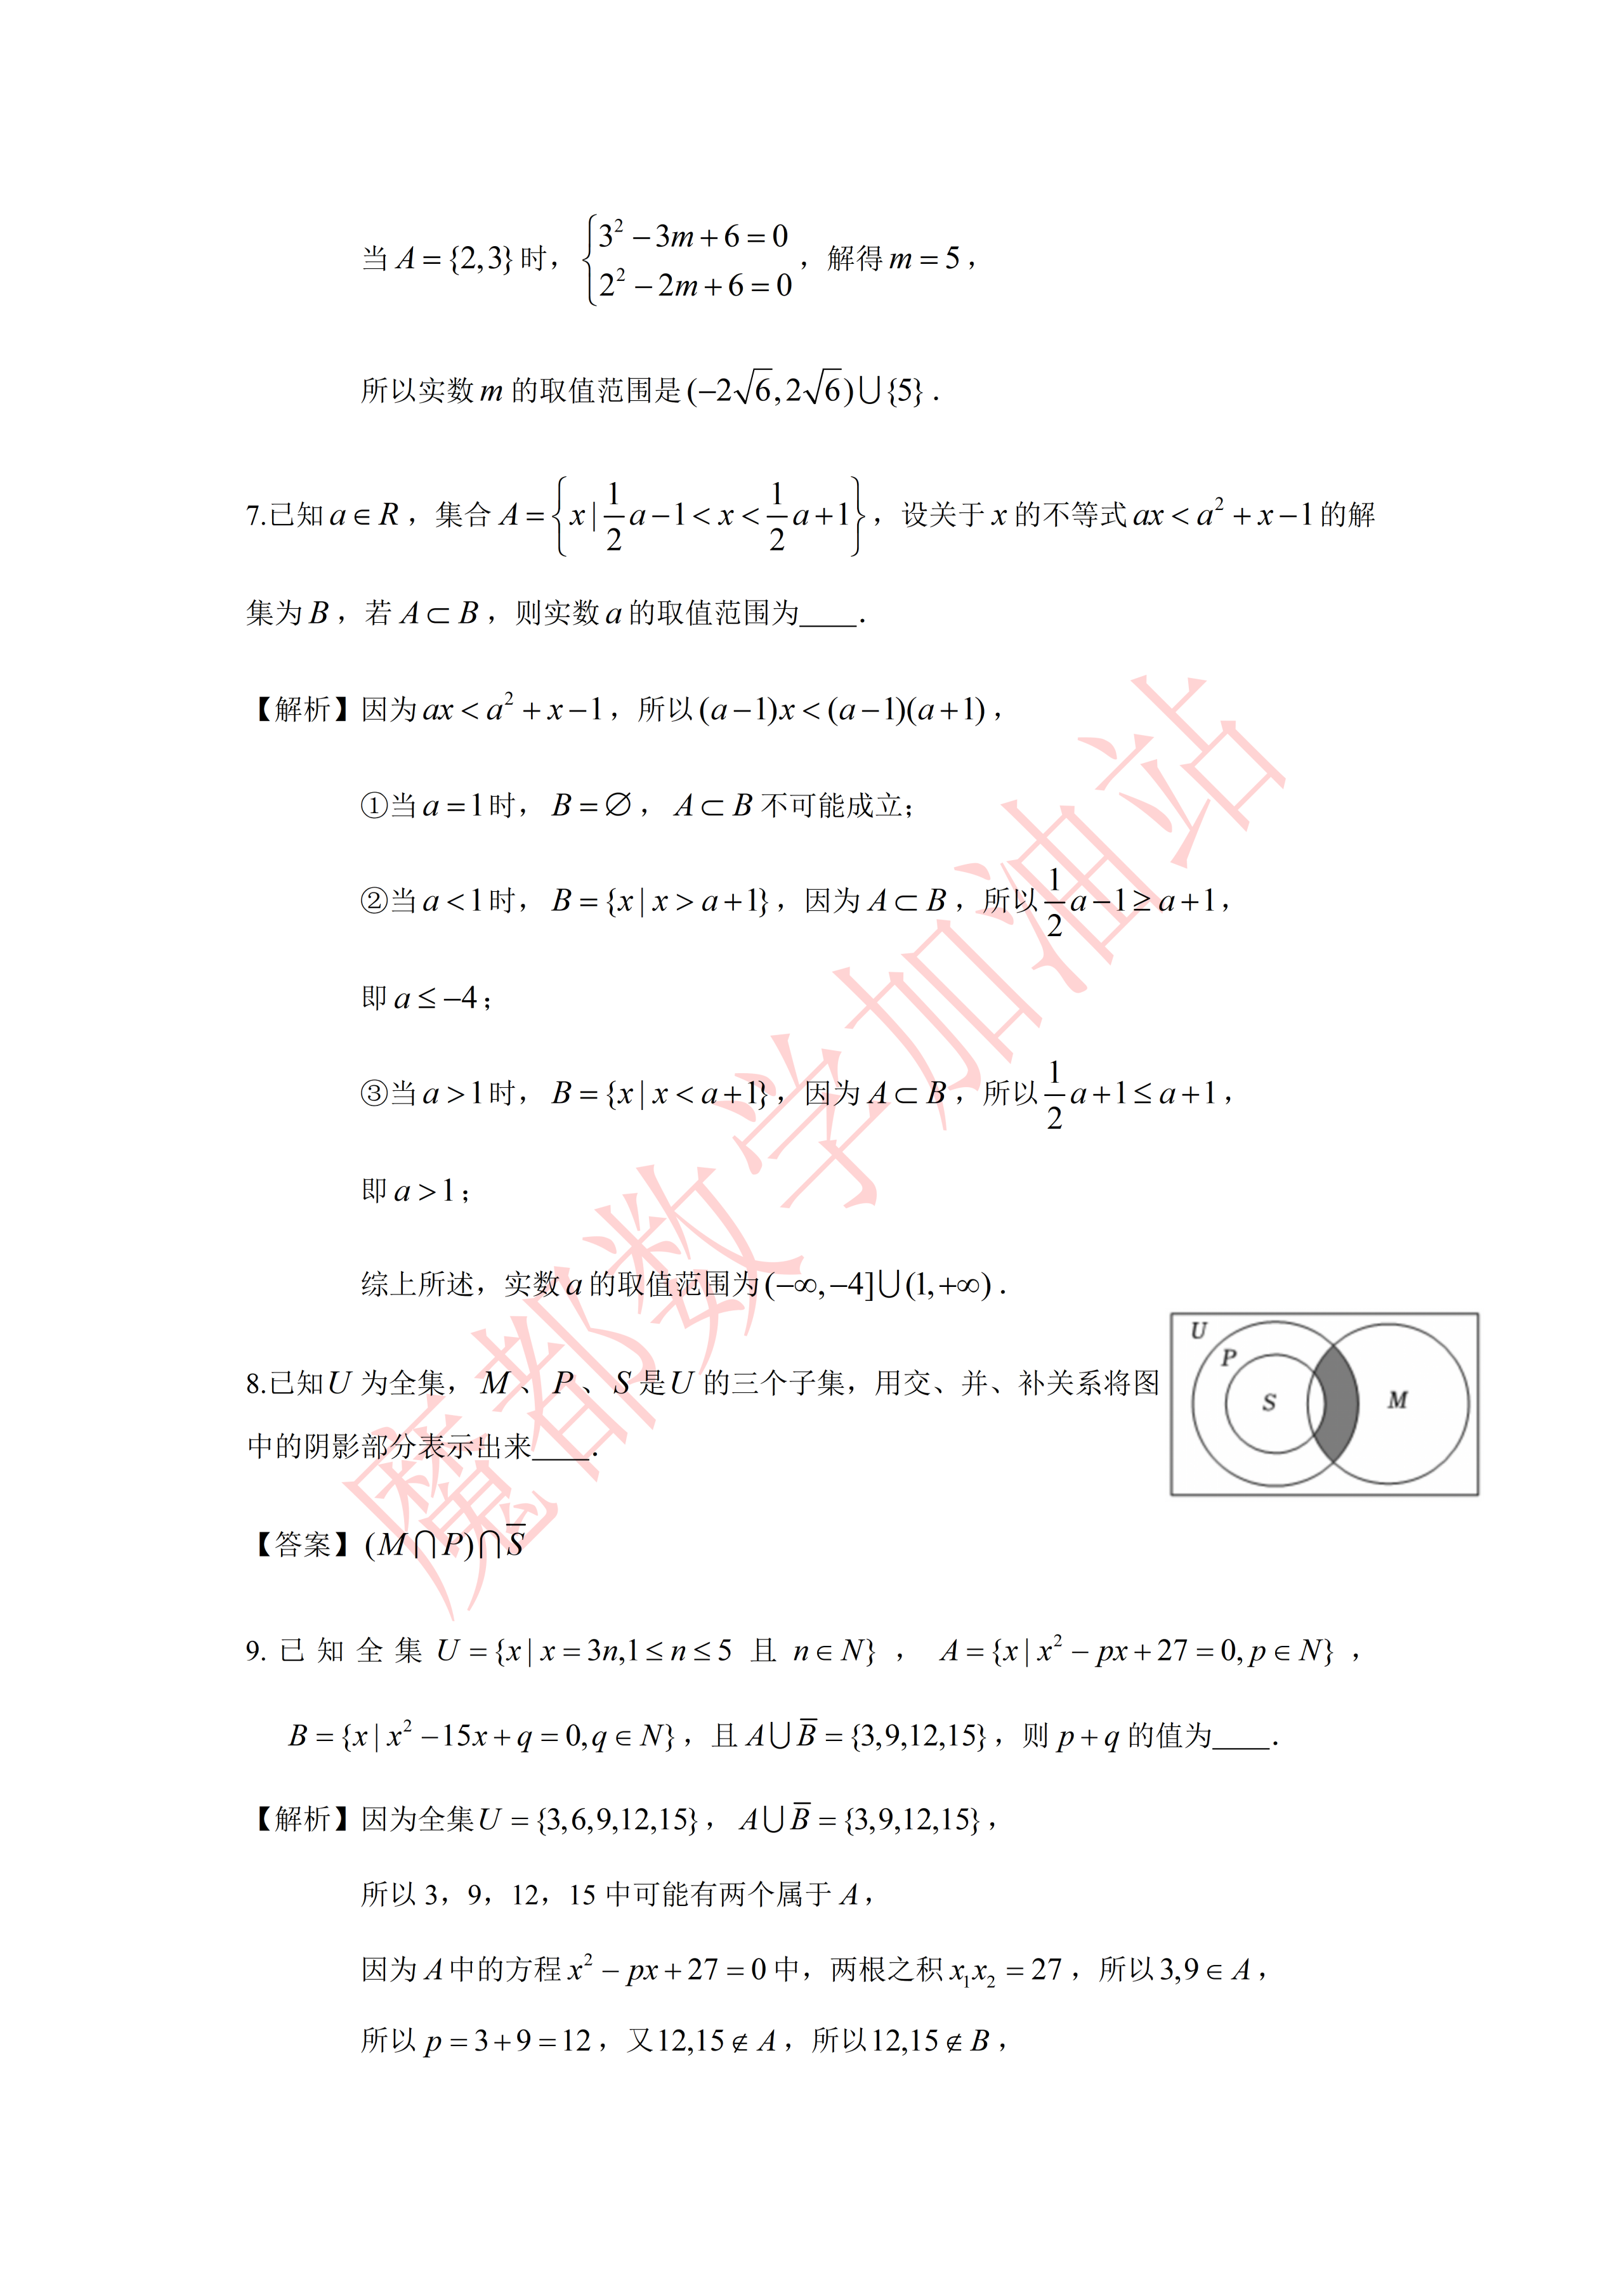
\includegraphics[width=.38\linewidth,trim=1835bp 1255bp 220bp 1565bp,clip]{../原图/高一49_华师大二附中_国庆作业1/02.png}
\end{center}

\ifanswer
\ans{$(M\cap P)\cap\overline S$}
\fi

\item 已知全集 $U=\{x\mid x=3n,1\leqslant n\leqslant5\text{ 且 }n\in\N\}$，$A=\{x\mid x^2-px+27=0,p\in\N\}$，$B=\{x\mid x^2-15x+q=0,q\in\N\}$，且 $A\cup\overline B=\{3,9,12,15\}$，则 $p+q$ 的值为\blankline[4.4em].

\ifanswer
\solbegin
\step{因为全集 $U=\{3,6,9,12,15\}$，$A\cup\overline B=\{3,9,12,15\}$，}
\step{所以 $3$、$9$、$12$、$15$ 中可能有两个属于 $A$，}
\step{因为 $A$ 中的方程 $x^2-px+27=0$ 中，两根之积 $x_1x_2=27$，所以 $3,9\in A$，}
\step{所以 $p=3+9=12$，又 $12,15\notin A$，所以 $12,15\notin B$，}
\step{因为 $B$ 中的方程 $x^2-15x+q=0$ 中，两根之和 $x_3+x_4=15$，所以 $6,9\in B$，}
\step{则 $q=6\times9=54$，所以 $p+q=66$.}
\solend
\fi

\item 已知集合 $A=\{x\mid x^2+(2a-3)x-3a=0,a\in\R,x\in\R\}$，集合 $B=\{x\mid x^2+(a-3)x+a^2-3a=0,a\in\R,x\in\R\}$，若 $A\neq B$，$A\cap B\neq\varnothing$，则 $A\cup B=$\blankline[4.4em].

\ifanswer
\solbegin
\step{设两个集合中的方程的公共解是 $b$，}
\step{由 $b^2+(2a-3)b-3a=b^2+(a-3)b+a^2-3a$，得 $ab=a^2$，}
\step{则 $a=0$ 或 $b=a$，}
\step{当 $a=0$ 时，不合题意，}
\step{当 $b=a$ 时，即两个方程的公共解为 $b=a$，}
\step{将 $b=a$ 代入方程，得 $a^2=2a$，$a=2$，}
\step{所以 $A=\{2,-3\}$，$B=\{-1,2\}$，所以 $A\cup B=\{-1,2,-3\}$.}
\solend
\fi

\item 已知一个有四个数字元素的集合 $S$，$S$ 的所有子集的元素和（空集的元素和认为是 $0$）的总和为 $16192$，则 $S$ 的元素之和等于\blankline[4.4em].

\ifanswer
\solbegin
\step{设 $S=\{a_1,a_2,a_3,a_4\}$，$S$ 的每个元素在所有子集中均出现 $2^3$ 次，}
\step{故 $(a_1+a_2+a_3+a_4)\cdot2^3=16192$，所以 $a_1+a_2+a_3+a_4=2024$，}
\step{故 $S$ 的元素之和等于 $2024$.}
\solend
\fi

\item 设 $P$ 为非空实数集满足：对任意给定的 $x,y\in P$（$x$、$y$ 可以相同），都有 $x+y\in P,x-y\in P,xy\in P$，则称 $P$ 为封闭集．关于封闭集有下列结论：

①集合 $P=\{-2,-1,0,1,2\}$ 为封闭集；

②集合 $P=\{x\mid x=2n,n\in\Z\}$ 为封闭集；

③若集合 $P_1$、$P_2$ 为封闭集，则 $P_1\cup P_2$ 为封闭集；

④若集合 $P$ 为封闭集，则一定有 $0\in P$；

⑤若集合 $P_1$、$P_2$ 为封闭集，则 $P_1\cap P_2$ 为封闭集.

其中正确结论的序号是\blankline[4.4em].

\ifanswer
\solbegin
\step{对于集合 $P=\{-2,-1,0,1,2\}$，取 $x=2$，$y=-2$，则 $x-y=2-(-2)=4\notin P$，}
\step{不满足封闭集的定义，所以①错误.}
\step{对于集合 $P=\{x\mid x=2n,n\in\Z\}$，设 $x=2n_1$，$y=2n_2$，$n_1,n_2\in\Z$.}
\step{$x+y=2n_1+2n_2=2(n_1+n_2)$，因为 $n_1+n_2\in\Z$，所以 $x+y\in P$.}
\step{$x-y=2n_1-2n_2=2(n_1-n_2)$，因为 $n_1-n_2\in\Z$，所以 $x-y\in P$.}
\step{$xy=2n_1\times2n_2=4n_1n_2=2(2n_1n_2)$，因为 $2n_1n_2\in\Z$，所以 $xy\in P$.}
\step{满足封闭集的定义，所以②正确.}
\step{令 $P_1=\{x\mid x=2n,n\in\Z\}$，$P_2=\{x\mid x=3n,n\in\Z\}$，都是封闭集.}
\step{$P_1\cup P_2$ 中，取 $x=2(x\in P_1)$，$y=3(y\in P_2)$，$x+y=5\notin P_1\cup P_2$，}
\step{不满足封闭集的定义，所以③错误.}
\step{因为对任意 $x\in P$，有 $x-x=0\in P$，}
\step{所以若集合 $P$ 为封闭集，则一定有 $0\in P$，所以④正确.}
\step{因为 $P_1$、$P_2$ 为封闭集，设 $x,y\in P_1\cap P_2$，则 $x,y\in P_1$ 且 $x,y\in P_2$.}
\step{因为 $P_1$ 是封闭集，所以 $x+y\in P_1,x-y\in P_1,xy\in P_1$.}
\step{因为 $P_2$ 是封闭集，所以 $x+y\in P_2,x-y\in P_2,xy\in P_2$.}
\step{所以 $x+y\in P_1\cap P_2,x-y\in P_1\cap P_2,xy\in P_1\cap P_2$，满足封闭集的定义，}
\step{所以⑤正确.}
\step{故正确的是②④⑤.}
\solend
\fi

\end{enumerate}

\bigsec{二、选择题}

\begin{enumerate}
\setcounter{enumi}{12}

\item 已知集合 $A=\{1,3,\sqrt m\}$，$B=\{1,m\}$，$B\subseteq A$，则 $m=$\mbox{（\quad）}

\keepwithprev
A. $0$ 或 $\sqrt3$\qquad B. $0$ 或 $3$

C. $1$ 或 $\sqrt3$\qquad D. $1$ 或 $3$

\ifanswer
\solbegin
\step{因为集合 $A=\{1,3,\sqrt m\}$，$B=\{1,m\}$，$B\subseteq A$，所以 $m=3$ 或 $m=\sqrt m$，}
\step{若 $m=3$，$A=\{1,3,\sqrt3\}$，$B=\{1,3\}$，满足 $B\subseteq A$，}
\step{若 $m=\sqrt m$，解得 $m=1$ 或 $m=0$，}
\step{①若 $m=0$，则 $A=\{1,3,0\}$，$B=\{1,0\}$，满足 $B\subseteq A$.}
\step{②若 $m=1$，则 $A$、$B$ 不满足集合中元素的互异性，舍去.}
\step{综上，$m=0$ 或 $m=3$．故选 $B$.}
\solend
\fi

\needvspace{10\baselineskip}

\item 设集合 $A$、$B$、$C$、$D$ 是全集 $X$ 的子集，$A\cap B\neq\varnothing$，$A\cap C\neq\varnothing$，则下列选项中正确的是\mbox{（\quad）}

\keepwithprev
A. 如果 $D\subset B$ 或 $D\subset C$，则 $D\cap A\neq\varnothing$

B. 如果 $D\subset A$，则 $\overline D\cap B\neq\varnothing$，$\overline D\cap C\neq\varnothing$

C. 如果 $A\subset D$，则 $\overline D\cap B=\varnothing$，$\overline D\cap C=\varnothing$

D. 上述各项都不正确

\ifanswer
\solbegin
\step{用韦恩图表示每个选项：}
\begin{center}
% 原图第 5 页解析配图（三联韦恩图）直接裁取（原卷排于选项 C、D 右侧）。
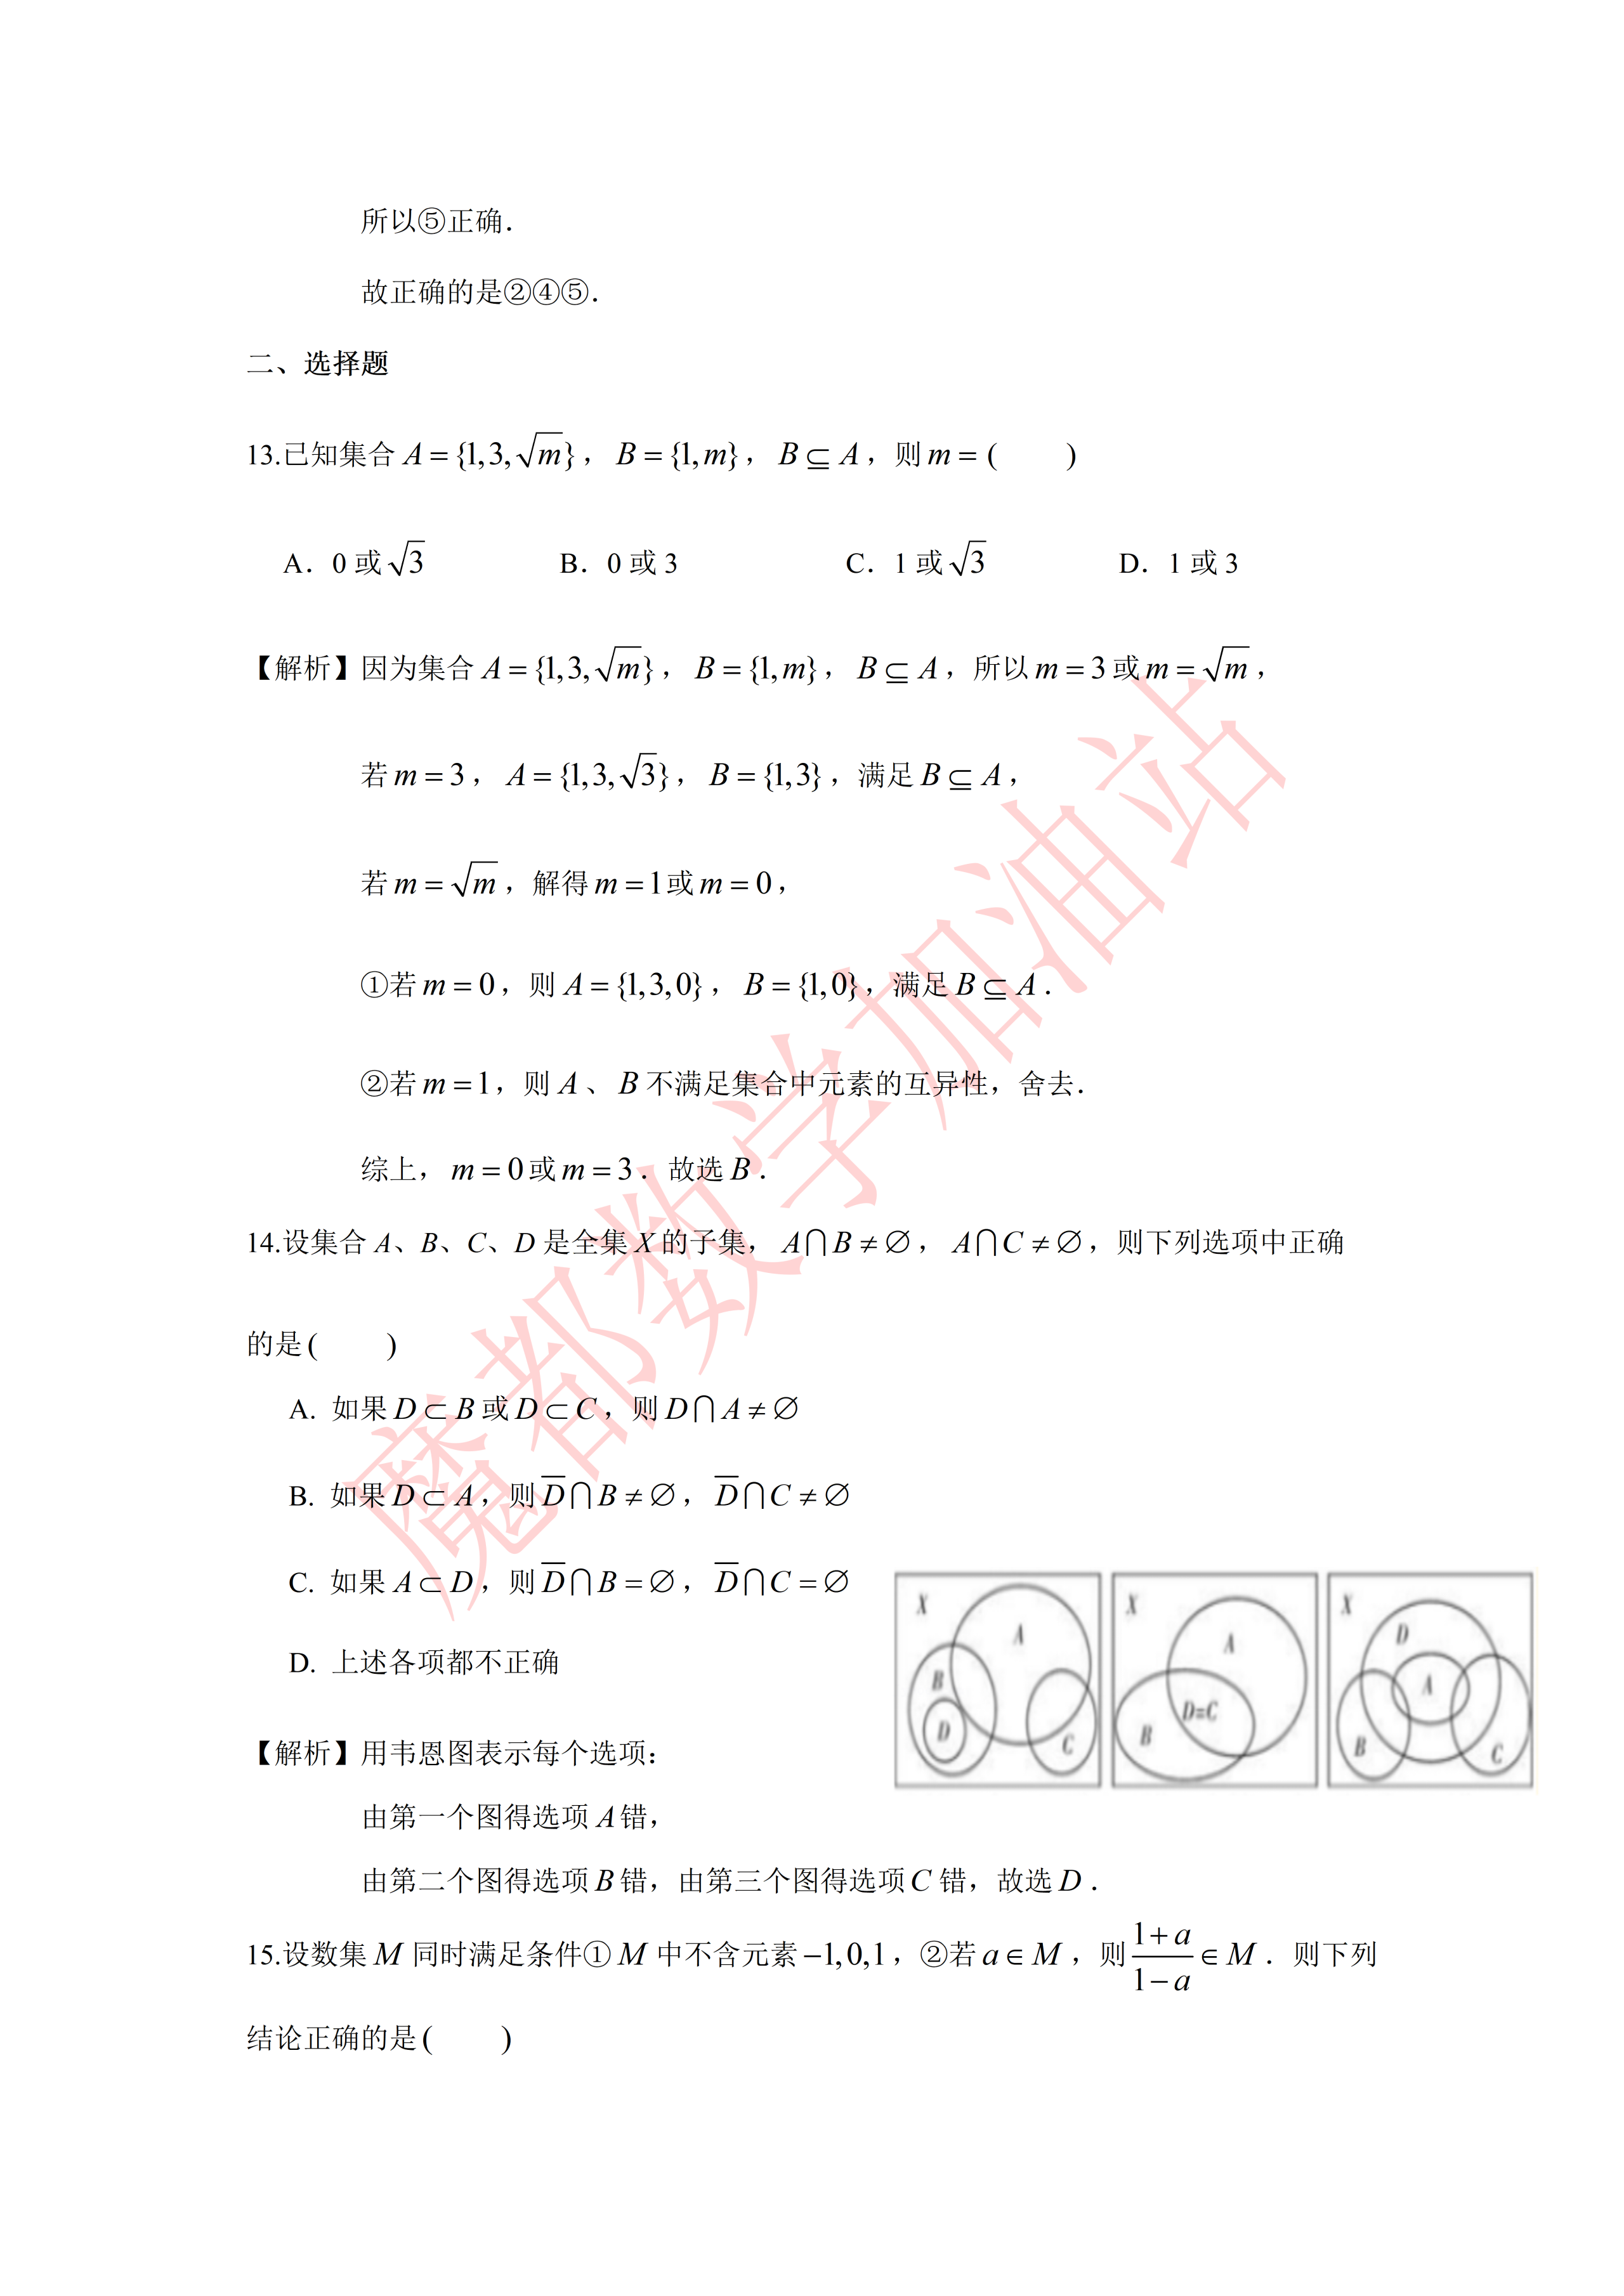
\includegraphics[width=.75\linewidth,trim=1400bp 790bp 135bp 1155bp,clip]{../原图/高一49_华师大二附中_国庆作业1/05.png}
\end{center}
\step{由第一个图得选项 $A$ 错，}
\step{由第二个图得选项 $B$ 错，由第三个图得选项 $C$ 错，故选 $D$.}
\solend
\fi

\item 设数集 $M$ 同时满足条件①$M$ 中不含元素 $-1$、$0$、$1$，②若 $a\in M$，则 $\dfrac{1+a}{1-a}\in M$．则下列结论正确的是\mbox{（\quad）}

\keepwithprev
A. 集合 $M$ 中至多有 $2$ 个元素\qquad B. 集合 $M$ 中至多有 $3$ 个元素

C. 集合 $M$ 中有且仅有 $4$ 个元素\qquad D. 集合 $M$ 中有无穷多个元素

\ifanswer
\solbegin
\step{若集合只含有一个元素，则 $\dfrac{1+a}{1-a}=a$，即 $1+a=a-a^2$，即 $-a^2=1$，不成立.}
\step{当 $a=3$ 时，$\dfrac{1+3}{1-3}=-2\in M$，所以 $\dfrac{1-2}{1+2}=-\dfrac13\in M$，所以 $\dfrac{1-\frac13}{1+\frac13}=\dfrac12\in M$，}
\step{所以 $\dfrac{1+\frac12}{1-\frac12}=3$，开始重复了，所以 $M=\left\{3,-2,-\dfrac13,\dfrac12\right\}$；}
\step{当 $a=2$ 时，$\dfrac{1+2}{1-2}=-3\in M$，所以 $\dfrac{1-3}{1+3}=-\dfrac12\in M$，所以 $\dfrac{1-\frac12}{1+\frac12}=\dfrac13\in M$，}
\step{所以 $\dfrac{1+\frac13}{1-\frac13}=2$，开始重复了，所以 $M=\left\{2,-3,-\dfrac12,-\dfrac13\right\}$，}
\step{此时也只要四个元素；}
\step{当 $a=\dfrac34\in M$，则 $7\in M$，若 $7\in M$，则 $-\dfrac43\in M$，}
\step{若 $-\dfrac43\in M$，则 $-\dfrac17\in M$，若 $-\dfrac17\in M$，有 $\dfrac34\in M$，}
\step{由归纳推理得，集合 $M$ 中有且仅有 $4$ 个元素．故选 $C$.}
\solend
\fi

\item 已知集合 $M=\{x\mid x\in\N,0<x\leqslant15\}$，$A_1$、$A_2$、$A_3$ 满足：①$A_1\cup A_2\cup A_3=M$；②每个集合都恰有 $5$ 个元素．集合 $A_i$（$i=1,2,3$）中最大元素与最小元素之和称为 $A_i$ 的特征数，记为 $X_i$（$i=1,2,3$），则 $X_1+X_2+X_3$ 的值不可能为\mbox{（\quad）}

\keepwithprev
A. $37$\qquad B. $39$\qquad C. $48$\qquad D. $57$

\ifanswer
\solbegin
\step{因为集合 $M=\{x\mid x\in\N,0<x\leqslant15\}=\{1,2,3,\cdots,15\}$，}
\step{又因为集合 $A_1$、$A_2$、$A_3$ 中，每个集合恰有 $5$ 个元素，}
\step{且 $A_1\cup A_2\cup A_3=M$ 有 $15$ 个元素，所以集合 $A_1$、$A_2$、$A_3$ 中没有重复元素，}
\step{因为 $1$ 是集合 $M$ 中数值最小的元素，$15$ 是集合 $M$ 中数值最大的元素，}
\step{所以在 $A_i$ 的特征数构成中，必有 $1$ 和 $15$，不妨设 $1\in A_1$，$15\in A_1$，}
\step{要使 $X_1+X_2+X_3$ 最大，则应该在集合 $A_1$ 中首先放置数值较小的元素，}
\step{即 $A_1=\{1,2,3,4,15\}$，所以 $5$ 与 $14$ 是剩下元素中数值最小或最大的元素，}
\step{同理，不妨设 $5\in A_2$，$14\in A_2$，接着在 $A_2$ 中再次放置数值较小的元素，}
\step{即 $A_2=\{5,6,7,8,14\}$，则 $A_3=\{9,10,11,12,13\}$，}
\step{此时 $X_1+X_2+X_3$ 有最大值为 $1+15+5+14+9+13=57$，}
\step{即 $X_1+X_2+X_3\leqslant57$；}
\step{要使 $X_1+X_2+X_3$ 最小，则在集合 $A_1$ 中首先放置数值较大的元素，}
\step{即 $A_1=\{1,12,13,14,15\}$，所以 $2$ 与 $11$ 是剩下元素中数值最小或最大的元素，}
\step{同理，不妨设 $2\in A_2$，$11\in A_2$，接着在 $A_2$ 中再次放置数值较大的元素，}
\step{即 $A_2=\{2,8,9,10,11\}$，则 $A_3=\{3,4,5,6,7\}$，}
\step{此时 $X_1+X_2+X_3$ 有最小值为 $1+15+2+11+3+7=39$，}
\step{即 $X_1+X_2+X_3\geqslant39$，}
\step{综上，$39\leqslant X_1+X_2+X_3\leqslant57$，故选 $A$.}
\solend
\fi

\end{enumerate}

\bigsec{三、解答题}

\begin{enumerate}
\setcounter{enumi}{16}

\item 已知全集为 $\R$，集合 $A=\{x\mid y=\sqrt{(2+x)(4-x)}\}$，$B=\{x\mid-1<x<m+1\}$.

\begin{enumerate}[label=(\arabic*)]
\item 若 $m=4$，求 $A\cup B$、$\overline A\cap B$；
\item 若 $B\subseteq A$，求实数 $m$ 的取值范围.
\end{enumerate}

\ifanswer
\solbegin
\stepm{(1)}{集合 $A=\{x\mid y=\sqrt{(2+x)(4-x)}\}=\{x\mid-2\leqslant x\leqslant4\}$，}
\step{当 $m=4$ 时，$B=\{x\mid-1<x<5\}$.}
\step{所以 $A\cup B=[-2,5)$，$\overline A=\{x\mid x<-2\text{ 或 }x>4\}$，$\overline A\cap B=(4,5)$.}
\stepm{(2)}{因为 $B\subseteq A$，}
% 原卷如此，照录未改（第 17 题(2)解析两处"当 C=∅／当 C≠∅"应为 B，本卷并无集合 C）
\step{当 $C=\varnothing$ 时，$m\leqslant-2$，$B\subseteq A$ 成立；}
\step{当 $C\neq\varnothing$ 时，$m>-2$，$-1<m+1\leqslant4$，解得 $-2<m\leqslant3$，}
\step{综上，$m\leqslant3$，所以实数 $m$ 的取值范围是 $(-\infty,3]$.}
\solend
\fi

\ansspace[6]

\item 用反证法证明：若 $a$、$b$、$c\in\R$，且 $x=a^2-2b+1$，$y=b^2-2c+1$，$z=c^2-2a+1$，则 $x$、$y$、$z$ 中至少有一个不小于 $0$.

\ifanswer
\solbegin
\step{假设 $x$、$y$、$z$ 均小于 $0$，即 $x=a^2-2b+1<0$①，$y=b^2-2c+1<0$②，}
\step{$z=c^2-2a+1<0$③，①$+$②$+$③得 $x+y+z=(a-1)^2+(b-1)^2+(c-1)^2<0$，}
\step{这与 $(a-1)^2+(b-1)^2+(c-1)^2\geqslant0$ 矛盾，则假设不成立，}
\step{所以 $x$、$y$、$z$ 中至少有一个不小于 $0$，得证.}
\solend
\fi

\ansspace[5]

\item 已知全集为 $\R$，实数 $a$、$b$ 满足 $a\neq b$，集合 $M=\{x\mid x^2-3x-4\leqslant0\}$，集合 $A=\{x\mid(x+a)(x+b)>0\}$，集合 $B=\{x\mid x^2+(a-2)x-2a>0\}$.

\begin{enumerate}[label=(\arabic*)]
\item 若 $\overline A=M$，求 $a$、$b$ 的值；
\item 若 $a>b>-1$，求 $A\cap B$；
\item 若 $a^2+a\in\overline B$，求 $a$ 的取值范围.
\end{enumerate}

\ifanswer
\solbegin
\stepm{(1)}{$M=\{x\mid x^2-3x-4\leqslant0\}=\{x\mid-1\leqslant x\leqslant4\}$，$A=\{x\mid(x+a)(x+b)\leqslant0\}$，}
\step{因为 $\overline A=M$，所以 $a=1$，$b=-4$ 或 $a=-4$，$b=1$.}
\stepm{(2)}{因为 $a>b>-1$，所以 $-a<-b<1$，所以 $A=\{x\mid x<-a\text{ 或 }x>-b\}$，}
\step{因为 $B=\{x\mid x^2+(a-2)x-2a>0\}=\{x\mid x<-a\text{ 或 }x>2\}$，}
\step{所以 $A\cap B=\{x\mid x<-a\text{ 或 }x>2\}$，}
\stepm{(3)}{$\overline B=\{x\mid(x-2)(x+a)\leqslant0\}$，}
% 原卷如此，照录未改（第 19 题(3)此处"a(a-1)((a-2)^2≤0"括号不配对；且由左式展开应为
% a(a-1)(a+2)^2≤0，与下句"解得 a=2 …[0,1]∪{2}"按 (a-2)^2 方自洽，见文件头清单第 2 条）
\step{由 $a^2+a\in\overline B$，得 $(a^2+a-2)(a^2+2a)\leqslant0\Leftrightarrow a(a-1)((a-2)^2\leqslant0$，}
\step{解得 $a=2$ 或 $0\leqslant a\leqslant1$，故 $a$ 的取值范围是 $[0,1]\cup\{2\}$.}
\solend
\fi

\ansspace[7]

\item 设数集 $A$ 由实数构成，若 $x\in A$（$x\neq1$ 且 $x\neq0$），则 $\dfrac{1}{1-x}\in A$.

\begin{enumerate}[label=(\arabic*)]
\item 若 $2\in A$，则 $A$ 中至少还有几个元素；
\item 集合 $A$ 是否为双元素集合？请说明理由；
\item 若 $A$ 中元素个数不超过 $8$ 个，所有元素的和为 $\dfrac{14}{3}$，且 $A$ 中有一个元素的平方等于所有元素的积，求集合 $A$.
\end{enumerate}

\ifanswer
\solbegin
\stepm{(1)}{若 $x\in A$，则 $\dfrac{1}{1-x}\in A$，又 $2\in A$，所以 $\dfrac{1}{1-2}=-1\in A$，}
\step{所以 $\dfrac{1}{1-(-1)}=\dfrac12\in A$，所以 $\dfrac{1}{1-\frac12}=2\in A$，}
% 原卷如此，照录未改（第 20 题(1)解析末句"2 个几个元素"衍一"几个"）
\step{所以 $A$ 中至少还有 $2$ 个几个元素；}
\stepm{(2)}{若 $x\in A$（$x\neq1$ 且 $x\neq0$），则 $\dfrac{1}{1-x}\in A$，}
\step{则 $\dfrac{1}{1-\frac{1}{1-x}}=\dfrac{1-x}{-x}\in A$，则 $\dfrac{1}{1-\frac{1-x}{-x}}=x\in A$}
\step{若 $A$ 为双元素集，则 $x=\dfrac{1}{1-x}$ 或 $x=\dfrac{1-x}{-x}$ 或 $\dfrac{1}{1-x}=\dfrac{1-x}{-x}$，均无解，}
\step{所以 $A$ 不可能为双元素集；}
\stepm{(3)}{由 $x\in A$，$\dfrac{1}{1-x}\in A$，得 $\dfrac{1}{1-\frac{1}{1-x}}=\dfrac{x-1}{x}\in A$，得 $\dfrac{1}{1-\frac{x-1}{x}}=x\in A$，}
\step{所以 $\left\{x,\dfrac{1}{1-x},\dfrac{x-1}{x}\right\}\subseteq A$，而 $x\cdot\dfrac{1}{1-x}\cdot\dfrac{x-1}{x}=-1$，}
\step{$A$ 中元素个数为 $3$ 的倍数，则 $A$ 中元素只有 $6$ 个，}
\step{因为 $A$ 中有一个元素的平方等于所有元素的积，}
\step{不妨设 $x^2=1$，解得 $x=-1$ 或 $x=1$（舍），则 $-1$、$\dfrac12$、$2\in A$，}
\step{所以 $-1+\dfrac12+2+m+\dfrac{1}{1-m}+\dfrac{m-1}{m}=\dfrac{14}{3}$，解得 $m=-\dfrac12$ 或 $m=3$ 或 $m=\dfrac23$，}
\step{所以 $A=\left\{\dfrac12,2,-1,-\dfrac12,3,\dfrac23\right\}$.}
\solend
\fi

\ansspace[9]

% 原卷如此，照录未改（第 21 题题干"21.求已知集合"之"求"字疑衍；"任意两个元素 a_i a_j"
% 疑脱逗号；"|a_i-a_j|≥1/30 则称"之前疑脱标点，见文件头清单第 4 条）
\item 求已知集合 $M=\left\{\dfrac{1}{k}\middle|1\leqslant k\leqslant100\text{ 且 }k\in\N^{*}\right\}$，$A=\{a_1,a_2,\cdots,a_n\}$，其中 $n\in\N^{*}$，且 $n\geqslant2$．若 $A\subseteq\N$，且对集合 $A$ 中的任意两个元素 $a_ia_j$，$i\neq j$ 都有 $|a_i-a_j|\geqslant\dfrac{1}{30}$ 则称集合 $A$ 有性质 $P$.

\begin{enumerate}[label=(\arabic*)]
\item 判断集合 $\left\{\dfrac13,\dfrac14,\dfrac15,\dfrac16,\dfrac17\right\}$ 是否具有性质 $P$；
\item 若集合 $A=\{a_1,a_2,\cdots,a_n\}$ 具有性质 $P$.

①求证：$a_i-a_j$ 的最大值大于等于 $\dfrac{n-1}{30}$；

②求 $A$ 的元素个数 $n$ 的最大值.
\end{enumerate}

\ifanswer
\solbegin
\stepm{(1)}{集合为 $\left\{\dfrac13,\dfrac14,\dfrac15,\dfrac16,\dfrac17\right\}$，又 $\dfrac16-\dfrac17=\dfrac{1}{42}<\dfrac{1}{30}$，所以该集合不具有性质 $P$；}
\stepm{(2)}{①因为集合 $A=\{a_1,a_2,\cdots,a_n\}$ 具有性质 $P$，}
\step{不妨设 $a_1<a_2<a_3<\cdots<a_n$，则 $a_i-a_j\geqslant\dfrac{1}{30}$（$i>j$），}
\step{所以 $a_n-a_1=(a_n-a_{n-1})+(a_{n-1}-a_{n-2})+\cdots+(a_2-a_1)\geqslant\dfrac{n-1}{30}$，}
\step{故 $a_i-a_j$ 的最大值大于等于 $\dfrac{n-1}{30}$；}
% 原卷如此，照录未改（第 21 题(2)②首行"a_2-a_1≥(n-1)/30"：由①同款推理只能得
% a_2-a_1≥1/30，见文件头清单第 5 条）
\step{②$A=\{a_1,a_2,\cdots,a_n\}$，不妨设 $a_1<a_2<a_3<\cdots<a_n$，}
\step{要使 $A$ 的元素个数 $n$ 最大，}
\step{则 $A$ 中的元素满足 $a_n=\dfrac{1}{k}$，$a_{n-1}=\dfrac{1}{k+1}$，$\cdots$，$a_1=\dfrac{1}{k+n-1}$（$k\in\N^{*}$），}
\step{又由①得 $a_2-a_1=\dfrac{1}{k+n-2}-\dfrac{1}{k+n-1}\geqslant\dfrac{n-1}{30}$，}
\step{所以 $(k+n-2)(k+n-1)\leqslant30$，又 $a_n-a_{n-1}=\dfrac{1}{k}-\dfrac{1}{k+1}\geqslant\dfrac{1}{30}$，}
\step{所以 $k(k+1)\leqslant30$，所以 $1\leqslant k\leqslant5$（$k\in\N^{*}$），}
\step{当 $k=5$ 时，由 $(k+n-2)(k+n-1)\leqslant30$，解得 $n\leqslant2$，$n\in\N^{*}$；}
\step{当 $k=4$ 时，由 $(k+n-2)(k+n-1)\leqslant30$，解得 $n\leqslant3$，$n\in\N^{*}$；}
\step{当 $k=3$ 时，由 $(k+n-2)(k+n-1)\leqslant30$，解得 $n\leqslant4$，$n\in\N^{*}$；}
\step{当 $k=2$ 时，由 $(k+n-2)(k+n-1)\leqslant30$，解得 $n\leqslant5$，$n\in\N^{*}$；}
\step{当 $k=1$ 时，由 $(k+n-2)(k+n-1)\leqslant30$，解得 $n\leqslant6$，$n\in\N^{*}$.}
\step{故 $A$ 的元素个数 $n$ 的最大值为 $6$，此时集合 $A=\left\{1,\dfrac12,\dfrac13,\cdots,\dfrac16\right\}$.}
\solend
\fi

\ansspace*[10]

\end{enumerate}

\end{document}
"
% 紧凑版：xelatex "\def\iscompact{1}% 高一49_华师大二附中_国庆作业1.tex
%   —— 高一上数学"2026-2027 年华师大二附中高一上国庆作业 1"（讲评版）
% 试卷版：xelatex 高一49_华师大二附中_国庆作业1.tex
% 答案版：xelatex "\def\isanswer{1}% 高一49_华师大二附中_国庆作业1.tex
%   —— 高一上数学"2026-2027 年华师大二附中高一上国庆作业 1"（讲评版）
% 试卷版：xelatex 高一49_华师大二附中_国庆作业1.tex
% 答案版：xelatex "\def\isanswer{1}% 高一49_华师大二附中_国庆作业1.tex
%   —— 高一上数学"2026-2027 年华师大二附中高一上国庆作业 1"（讲评版）
% 试卷版：xelatex 高一49_华师大二附中_国庆作业1.tex
% 答案版：xelatex "\def\isanswer{1}\input{高一49_华师大二附中_国庆作业1.tex}"
% 紧凑版：xelatex "\def\iscompact{1}\input{高一49_华师大二附中_国庆作业1.tex}"
%
% 原始材料：微信公众号"魔都数学加油站"文章，作者破晓，连载"27学年高一49"；
% 原文标题"27学年高一49——2026-2027年上海市华师大二附中高一上国庆作业1集合与逻辑、
% 等式与不等式的性质"；页面用 JS 渲染，未见明确发布日期（页内时间戳 ≈ 2026-10-05 21:37）；
% 原文链接：https://mp.weixin.qq.com/s/XxZTOBVQslK5cZm2_BbhOg。
% 正文为 11 张 PNG 页：第 01、03、04、06、07、08、09 页 4762×6735，
% 第 02、05、10、11 页 2560×3620，均按页序读取；粉色斜排"魔都数学加油站"为卷面水印，
% 与公众号页脚一并未录入。全卷 11 页均为试卷页，无二维码/宣传页。
%
% 题号与分节：原文自第 3 题起编，填空题 3—12、选择题 13—16、解答题 17—21，共 19 题。
% 讲评版：原卷每题下直接印【答案】或【解析】——只印【答案】的 3 题（第 3、5、8 题），
% 其余 16 题均只印【解析】；解析行数已逐题按印刷行照录（一条 \step＝原卷一个印刷行）。
%
% 卷首标题：照卷面印作"2026-2027 年华师大二附中高一上国庆作业 1"（公众号标题中的"上海市"
% 卷面没有，本稿照卷面），年份区间按全稿惯例排 en dash；副标题照卷面自印的
% "集合与逻辑单元综合检测"（原卷页首标题行下方即印此行，故不另按模块口径拟名）。
% 副标题依据：全卷 19 题均为集合与常用逻辑用语内容——集合类 15 题（6—17、19—21 中除
% 反证法题外），逻辑/命题类 3 题（第 3 题否定形式、第 4 题充要条件、第 5 题反证法假设），
% 反证法证明 1 题（第 18 题）；全卷无不等式求解题，公众号标题中"等式与不等式的性质"
% 与卷面实际内容不符。
%
% 与原卷的排版差异：
%   ① 原文从第 3 题起，填空题为 3—12、选择题为 13—16、解答题为 17—21，本稿保留原题号；
%   ② 原卷每题下直接印【答案】/【解析】，本稿按全稿惯例置于答案版；只印【解析】的题
%      不另提 \ans{}（照 高一36 口径），只印【答案】的题仅给 \ans{}；
%   ③ 原卷第 8 题韦恩图排在题干右侧、第 14 题三联韦恩图排在选项（C、D）右侧，
%      本稿分别移至题干下方、解析首步之后居中排，均直接裁取原图页（02.png、05.png）；
%   ④ 数集记号原卷排作斜体/加粗 R、N、Z，本稿统一为 \R、\N、\Z、\N^*；
%      填空横线按全稿惯例排为 \blankline[4.4em]。
%
% 原卷笔误/存疑清单（均照录未改，正文中该处有 % 注）：
%   1. 第 17 题(2)解析两处"当 C=∅／当 C≠∅"应为 B（本卷并无集合 C）；
%   2. 第 19 题(3)解析"a(a-1)((a-2)^2≤0"括号不配对（多一枚左括号）；且由
%      (a^2+a-2)(a^2+2a)≤0 展开应为 a(a-1)(a+2)^2≤0，与原卷结论"解得 a=2 …
%      [0,1]∪{2}"恰按 (a-2)^2 自洽——因式分解与原式不符，结论按 (a-2)^2 自洽，均照录；
%   3. 第 20 题(1)解析末句"至少还有 2 个几个元素"衍一"几个"；
%   4. 第 21 题题干"21.求已知集合"之"求"字疑衍；"任意两个元素 a_i a_j"疑脱逗号；
%      "≥1/30 则称"之前疑脱标点；
%   5. 第 21 题(2)②解析"a_2-a_1≥(n-1)/30"：由①同款推理只能得 a_2-a_1≥1/30，
%      原卷如此，照录未改（后续 (k+n-2)(k+n-1)≤30 即按该行推得）。
%
\documentclass[a4paper,11pt]{article}
\usepackage{common}

\begin{document}

\examtitlest[3]{2026--2027 年华师大二附中高一上国庆作业 1}{集合与逻辑单元综合检测}

\bigsec{一、填空题}

\begin{enumerate}
\setcounter{enumi}{2}

\item “若 $x^2-x-2\leqslant0$，则 $-1\leqslant x\leqslant2$”的否定形式为\blankline[4.4em].

\ifanswer
\ans{若 $x^2-x-2>0$，则 $x<-1$ 或 $x>2$}
\fi

\item 已知 $p:|x-3|<5$，$q:1-a<x<2a-3$，且 $p$ 是 $q$ 的充分非必要条件，则实数 $a$ 的取值范围是\blankline[4.4em].

\ifanswer
\solbegin
\step{由 $|x-3|<5$ 得 $-2<x<8$，}
\step{又 $p$ 是 $q$ 的充分不必要条件，所以 $(-2,8)\subset(1-a,2a-3)$，}
\step{即 $\begin{cases}-2\geqslant1-a\\ 8\leqslant2a-3\\ (2a-3)-(1-a)\neq8-(-2)\end{cases}$，解得 $a\geqslant\dfrac{11}{2}$，实数 $a$ 的取值范围是 $\left[\dfrac{11}{2},+\infty\right)$.}
\solend
\fi

\item 用反证法证明命题“设 $a$、$b\in\R$，则方程 $a_1x^2+b_1x+c_1=0$ 与 $a_2x^2+b_2x+c_2=0$ 至少有一个实根”时要做的假设是\blankline[4.4em].

\ifanswer
\ans{假设 $a$、$b\in\R$，方程 $a_1x^2+b_1x+c_1=0$ 与 $a_2x^2+b_2x+c_2=0$ 都没有实根}
\fi

\item 设集合 $A=\{x\mid x^2-mx+6=0,x\in\R\}$，且 $A\cap\{2,3\}=A$，则实数 $m$ 的取值范围是\blankline[4.4em].

\ifanswer
\solbegin
\step{由 $A\cap\{2,3\}=A$，得 $A\subseteq\{2,3\}$，}
\step{当 $A=\varnothing$ 时，$\Delta=m^2-24<0$，解得 $-2\sqrt6<m<2\sqrt6$；}
\step{当 $A=\{2\}$ 时，$\begin{cases}2^2-2m+6=0\\ \Delta=m^2-24=0\end{cases}$，无解；}
\step{当 $A=\{3\}$ 时，$\begin{cases}3^2-3m+6=0\\ \Delta=m^2-24=0\end{cases}$，无解；}
\step{当 $A=\{2,3\}$ 时，$\begin{cases}3^2-3m+6=0\\ 2^2-2m+6=0\end{cases}$，解得 $m=5$，}
\step{所以实数 $m$ 的取值范围是 $(-2\sqrt6,2\sqrt6)\cup\{5\}$.}
\solend
\fi

\item 已知 $a\in\R$，集合 $A=\left\{x\middle|\dfrac12a-1<x<\dfrac12a+1\right\}$，设关于 $x$ 的不等式 $ax<a^2+x-1$ 的解集为 $B$，若 $A\subset B$，则实数 $a$ 的取值范围为\blankline[4.4em].

\ifanswer
\solbegin
\step{因为 $ax<a^2+x-1$，所以 $(a-1)x<(a-1)(a+1)$，}
\step{①当 $a=1$ 时，$B=\varnothing$，$A\subset B$ 不可能成立；}
\step{②当 $a<1$ 时，$B=\{x\mid x>a+1\}$，因为 $A\subset B$，所以 $\dfrac12a-1\geqslant a+1$，}
\step{即 $a\leqslant-4$；}
\step{③当 $a>1$ 时，$B=\{x\mid x<a+1\}$，因为 $A\subset B$，所以 $\dfrac12a+1\leqslant a+1$，}
\step{即 $a>1$；}
\step{综上所述，实数 $a$ 的取值范围为 $(-\infty,-4]\cup(1,+\infty)$.}
\solend
\fi

\needvspace{8\baselineskip}

\item 已知 $U$ 为全集，$M$、$P$、$S$ 是 $U$ 的三个子集，用交、并、补关系将图中的阴影部分表示出来\blankline[4.4em].

\begin{center}
% 原图第 2 页题旁韦恩图直接裁取（原卷排于题干右侧）。
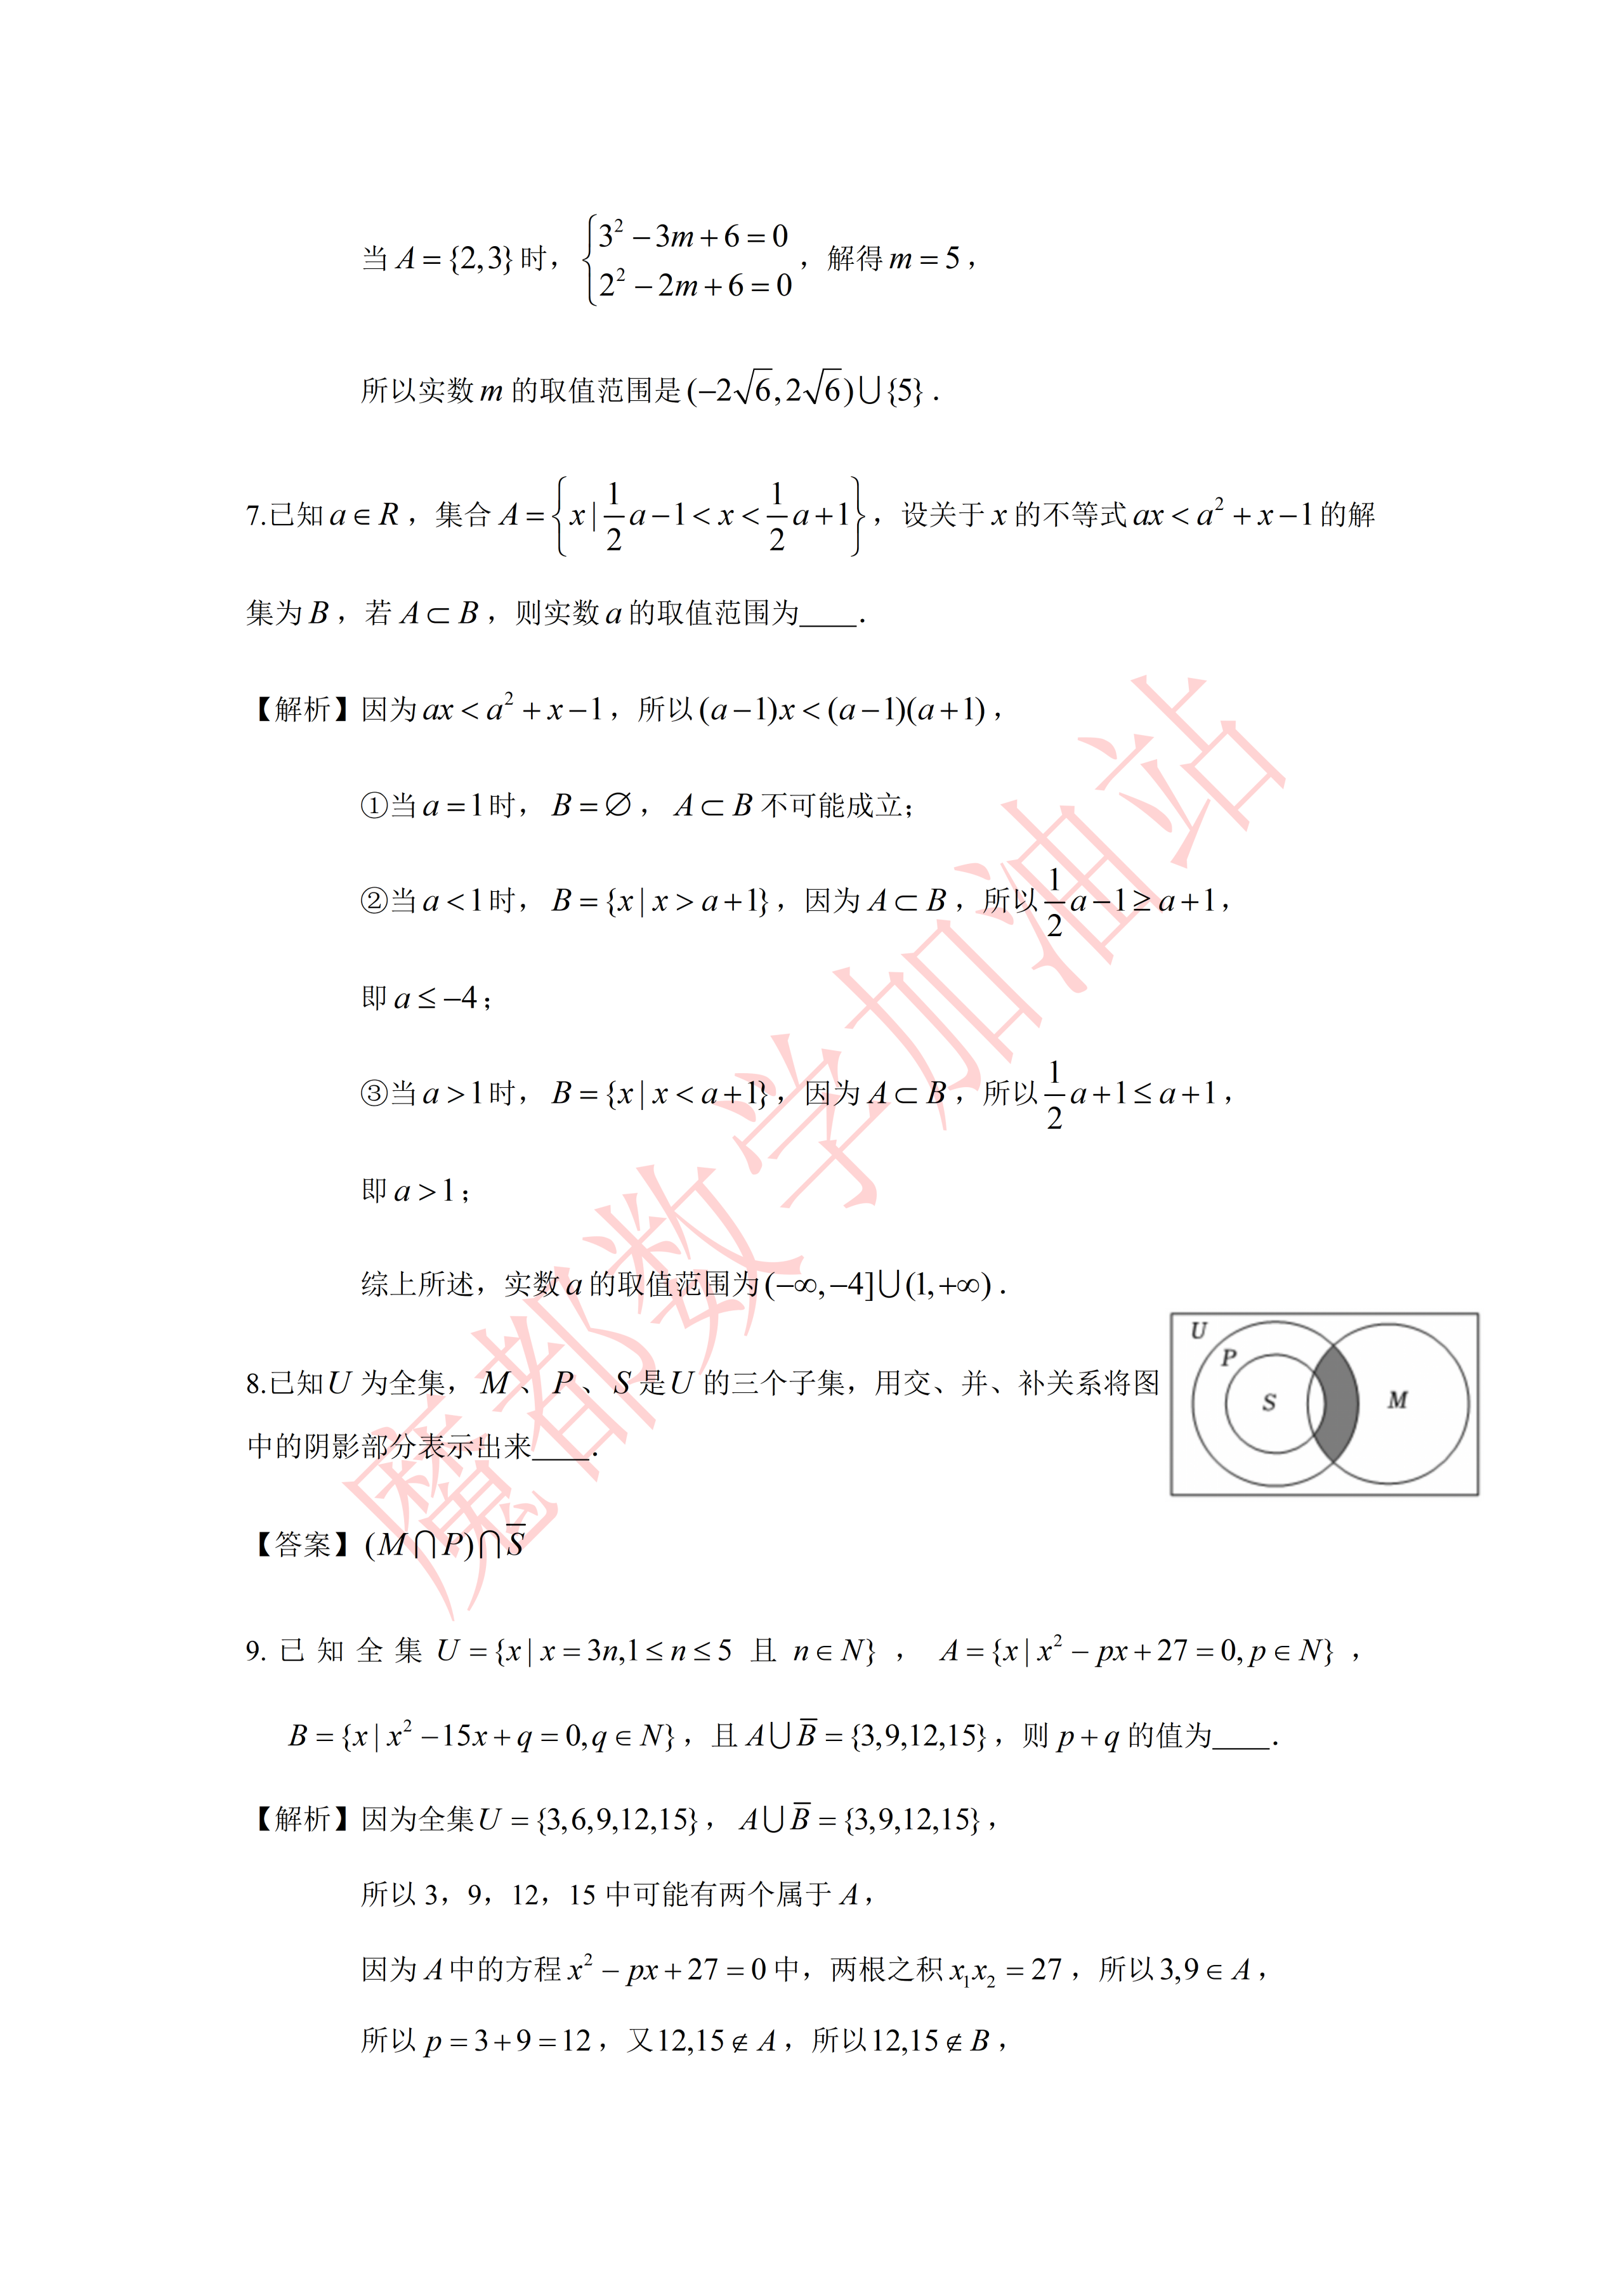
\includegraphics[width=.38\linewidth,trim=1835bp 1255bp 220bp 1565bp,clip]{../原图/高一49_华师大二附中_国庆作业1/02.png}
\end{center}

\ifanswer
\ans{$(M\cap P)\cap\overline S$}
\fi

\item 已知全集 $U=\{x\mid x=3n,1\leqslant n\leqslant5\text{ 且 }n\in\N\}$，$A=\{x\mid x^2-px+27=0,p\in\N\}$，$B=\{x\mid x^2-15x+q=0,q\in\N\}$，且 $A\cup\overline B=\{3,9,12,15\}$，则 $p+q$ 的值为\blankline[4.4em].

\ifanswer
\solbegin
\step{因为全集 $U=\{3,6,9,12,15\}$，$A\cup\overline B=\{3,9,12,15\}$，}
\step{所以 $3$、$9$、$12$、$15$ 中可能有两个属于 $A$，}
\step{因为 $A$ 中的方程 $x^2-px+27=0$ 中，两根之积 $x_1x_2=27$，所以 $3,9\in A$，}
\step{所以 $p=3+9=12$，又 $12,15\notin A$，所以 $12,15\notin B$，}
\step{因为 $B$ 中的方程 $x^2-15x+q=0$ 中，两根之和 $x_3+x_4=15$，所以 $6,9\in B$，}
\step{则 $q=6\times9=54$，所以 $p+q=66$.}
\solend
\fi

\item 已知集合 $A=\{x\mid x^2+(2a-3)x-3a=0,a\in\R,x\in\R\}$，集合 $B=\{x\mid x^2+(a-3)x+a^2-3a=0,a\in\R,x\in\R\}$，若 $A\neq B$，$A\cap B\neq\varnothing$，则 $A\cup B=$\blankline[4.4em].

\ifanswer
\solbegin
\step{设两个集合中的方程的公共解是 $b$，}
\step{由 $b^2+(2a-3)b-3a=b^2+(a-3)b+a^2-3a$，得 $ab=a^2$，}
\step{则 $a=0$ 或 $b=a$，}
\step{当 $a=0$ 时，不合题意，}
\step{当 $b=a$ 时，即两个方程的公共解为 $b=a$，}
\step{将 $b=a$ 代入方程，得 $a^2=2a$，$a=2$，}
\step{所以 $A=\{2,-3\}$，$B=\{-1,2\}$，所以 $A\cup B=\{-1,2,-3\}$.}
\solend
\fi

\item 已知一个有四个数字元素的集合 $S$，$S$ 的所有子集的元素和（空集的元素和认为是 $0$）的总和为 $16192$，则 $S$ 的元素之和等于\blankline[4.4em].

\ifanswer
\solbegin
\step{设 $S=\{a_1,a_2,a_3,a_4\}$，$S$ 的每个元素在所有子集中均出现 $2^3$ 次，}
\step{故 $(a_1+a_2+a_3+a_4)\cdot2^3=16192$，所以 $a_1+a_2+a_3+a_4=2024$，}
\step{故 $S$ 的元素之和等于 $2024$.}
\solend
\fi

\item 设 $P$ 为非空实数集满足：对任意给定的 $x,y\in P$（$x$、$y$ 可以相同），都有 $x+y\in P,x-y\in P,xy\in P$，则称 $P$ 为封闭集．关于封闭集有下列结论：

①集合 $P=\{-2,-1,0,1,2\}$ 为封闭集；

②集合 $P=\{x\mid x=2n,n\in\Z\}$ 为封闭集；

③若集合 $P_1$、$P_2$ 为封闭集，则 $P_1\cup P_2$ 为封闭集；

④若集合 $P$ 为封闭集，则一定有 $0\in P$；

⑤若集合 $P_1$、$P_2$ 为封闭集，则 $P_1\cap P_2$ 为封闭集.

其中正确结论的序号是\blankline[4.4em].

\ifanswer
\solbegin
\step{对于集合 $P=\{-2,-1,0,1,2\}$，取 $x=2$，$y=-2$，则 $x-y=2-(-2)=4\notin P$，}
\step{不满足封闭集的定义，所以①错误.}
\step{对于集合 $P=\{x\mid x=2n,n\in\Z\}$，设 $x=2n_1$，$y=2n_2$，$n_1,n_2\in\Z$.}
\step{$x+y=2n_1+2n_2=2(n_1+n_2)$，因为 $n_1+n_2\in\Z$，所以 $x+y\in P$.}
\step{$x-y=2n_1-2n_2=2(n_1-n_2)$，因为 $n_1-n_2\in\Z$，所以 $x-y\in P$.}
\step{$xy=2n_1\times2n_2=4n_1n_2=2(2n_1n_2)$，因为 $2n_1n_2\in\Z$，所以 $xy\in P$.}
\step{满足封闭集的定义，所以②正确.}
\step{令 $P_1=\{x\mid x=2n,n\in\Z\}$，$P_2=\{x\mid x=3n,n\in\Z\}$，都是封闭集.}
\step{$P_1\cup P_2$ 中，取 $x=2(x\in P_1)$，$y=3(y\in P_2)$，$x+y=5\notin P_1\cup P_2$，}
\step{不满足封闭集的定义，所以③错误.}
\step{因为对任意 $x\in P$，有 $x-x=0\in P$，}
\step{所以若集合 $P$ 为封闭集，则一定有 $0\in P$，所以④正确.}
\step{因为 $P_1$、$P_2$ 为封闭集，设 $x,y\in P_1\cap P_2$，则 $x,y\in P_1$ 且 $x,y\in P_2$.}
\step{因为 $P_1$ 是封闭集，所以 $x+y\in P_1,x-y\in P_1,xy\in P_1$.}
\step{因为 $P_2$ 是封闭集，所以 $x+y\in P_2,x-y\in P_2,xy\in P_2$.}
\step{所以 $x+y\in P_1\cap P_2,x-y\in P_1\cap P_2,xy\in P_1\cap P_2$，满足封闭集的定义，}
\step{所以⑤正确.}
\step{故正确的是②④⑤.}
\solend
\fi

\end{enumerate}

\bigsec{二、选择题}

\begin{enumerate}
\setcounter{enumi}{12}

\item 已知集合 $A=\{1,3,\sqrt m\}$，$B=\{1,m\}$，$B\subseteq A$，则 $m=$\mbox{（\quad）}

\keepwithprev
A. $0$ 或 $\sqrt3$\qquad B. $0$ 或 $3$

C. $1$ 或 $\sqrt3$\qquad D. $1$ 或 $3$

\ifanswer
\solbegin
\step{因为集合 $A=\{1,3,\sqrt m\}$，$B=\{1,m\}$，$B\subseteq A$，所以 $m=3$ 或 $m=\sqrt m$，}
\step{若 $m=3$，$A=\{1,3,\sqrt3\}$，$B=\{1,3\}$，满足 $B\subseteq A$，}
\step{若 $m=\sqrt m$，解得 $m=1$ 或 $m=0$，}
\step{①若 $m=0$，则 $A=\{1,3,0\}$，$B=\{1,0\}$，满足 $B\subseteq A$.}
\step{②若 $m=1$，则 $A$、$B$ 不满足集合中元素的互异性，舍去.}
\step{综上，$m=0$ 或 $m=3$．故选 $B$.}
\solend
\fi

\needvspace{10\baselineskip}

\item 设集合 $A$、$B$、$C$、$D$ 是全集 $X$ 的子集，$A\cap B\neq\varnothing$，$A\cap C\neq\varnothing$，则下列选项中正确的是\mbox{（\quad）}

\keepwithprev
A. 如果 $D\subset B$ 或 $D\subset C$，则 $D\cap A\neq\varnothing$

B. 如果 $D\subset A$，则 $\overline D\cap B\neq\varnothing$，$\overline D\cap C\neq\varnothing$

C. 如果 $A\subset D$，则 $\overline D\cap B=\varnothing$，$\overline D\cap C=\varnothing$

D. 上述各项都不正确

\ifanswer
\solbegin
\step{用韦恩图表示每个选项：}
\begin{center}
% 原图第 5 页解析配图（三联韦恩图）直接裁取（原卷排于选项 C、D 右侧）。
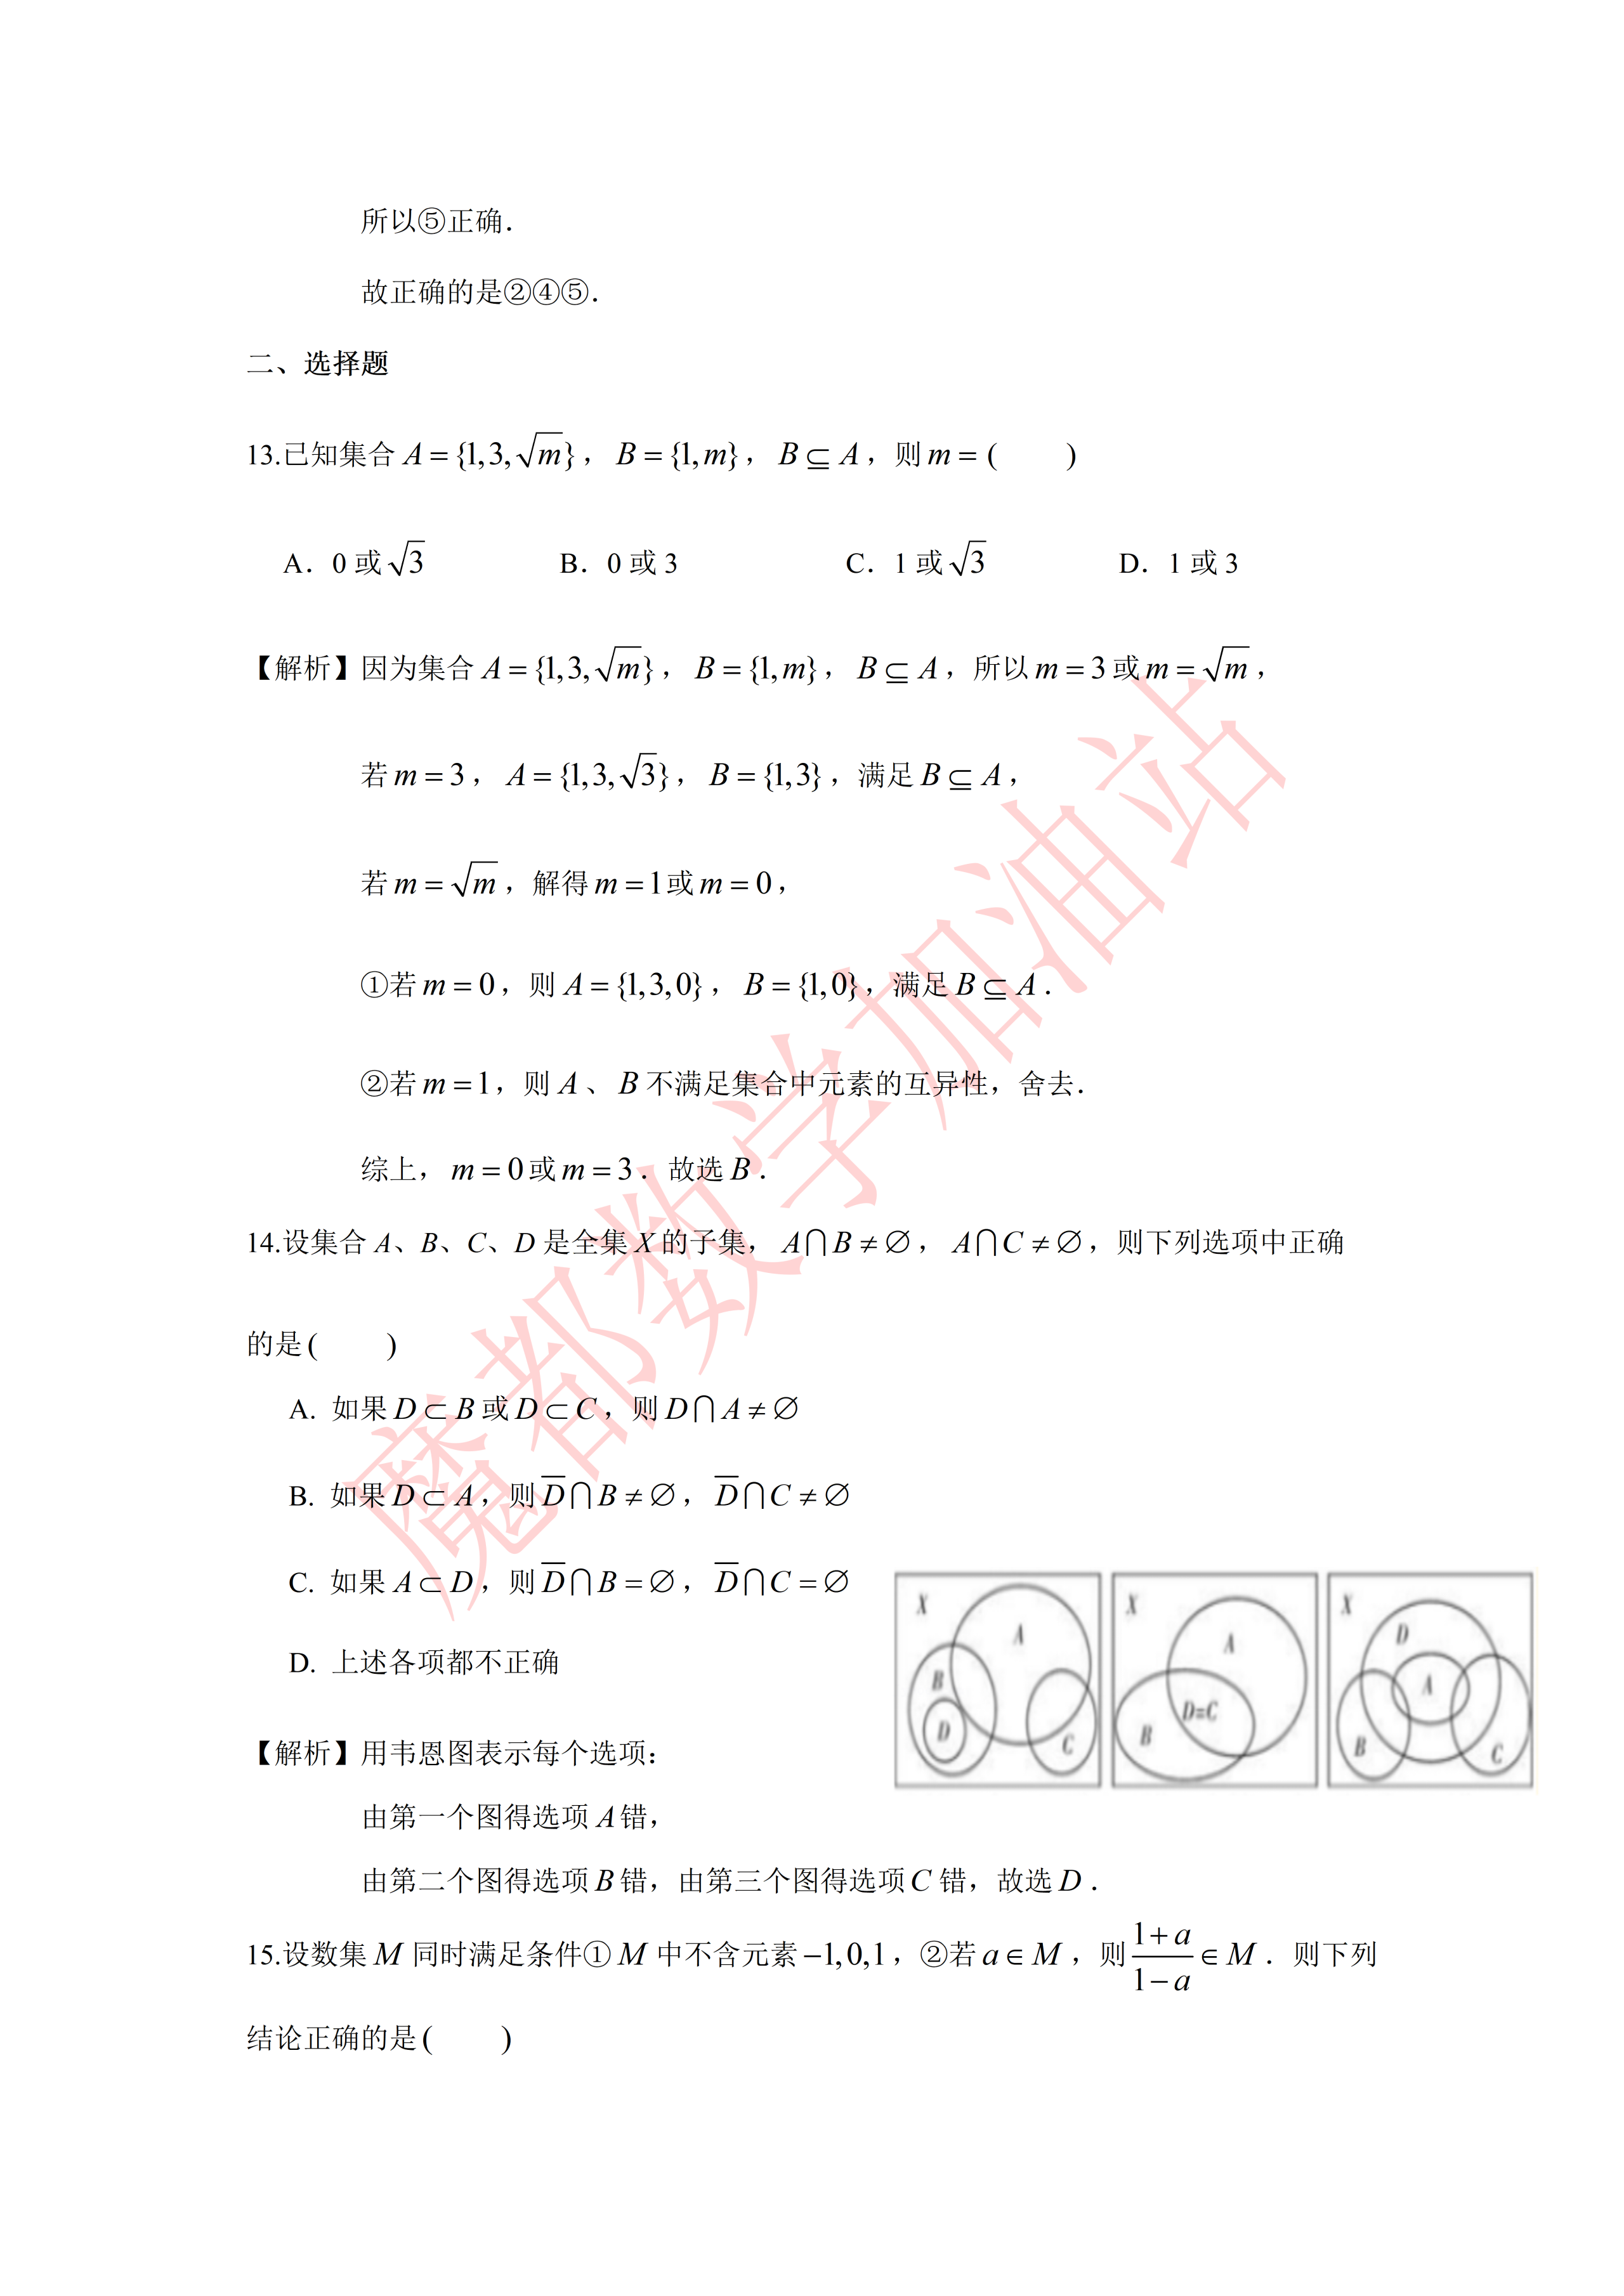
\includegraphics[width=.75\linewidth,trim=1400bp 790bp 135bp 1155bp,clip]{../原图/高一49_华师大二附中_国庆作业1/05.png}
\end{center}
\step{由第一个图得选项 $A$ 错，}
\step{由第二个图得选项 $B$ 错，由第三个图得选项 $C$ 错，故选 $D$.}
\solend
\fi

\item 设数集 $M$ 同时满足条件①$M$ 中不含元素 $-1$、$0$、$1$，②若 $a\in M$，则 $\dfrac{1+a}{1-a}\in M$．则下列结论正确的是\mbox{（\quad）}

\keepwithprev
A. 集合 $M$ 中至多有 $2$ 个元素\qquad B. 集合 $M$ 中至多有 $3$ 个元素

C. 集合 $M$ 中有且仅有 $4$ 个元素\qquad D. 集合 $M$ 中有无穷多个元素

\ifanswer
\solbegin
\step{若集合只含有一个元素，则 $\dfrac{1+a}{1-a}=a$，即 $1+a=a-a^2$，即 $-a^2=1$，不成立.}
\step{当 $a=3$ 时，$\dfrac{1+3}{1-3}=-2\in M$，所以 $\dfrac{1-2}{1+2}=-\dfrac13\in M$，所以 $\dfrac{1-\frac13}{1+\frac13}=\dfrac12\in M$，}
\step{所以 $\dfrac{1+\frac12}{1-\frac12}=3$，开始重复了，所以 $M=\left\{3,-2,-\dfrac13,\dfrac12\right\}$；}
\step{当 $a=2$ 时，$\dfrac{1+2}{1-2}=-3\in M$，所以 $\dfrac{1-3}{1+3}=-\dfrac12\in M$，所以 $\dfrac{1-\frac12}{1+\frac12}=\dfrac13\in M$，}
\step{所以 $\dfrac{1+\frac13}{1-\frac13}=2$，开始重复了，所以 $M=\left\{2,-3,-\dfrac12,-\dfrac13\right\}$，}
\step{此时也只要四个元素；}
\step{当 $a=\dfrac34\in M$，则 $7\in M$，若 $7\in M$，则 $-\dfrac43\in M$，}
\step{若 $-\dfrac43\in M$，则 $-\dfrac17\in M$，若 $-\dfrac17\in M$，有 $\dfrac34\in M$，}
\step{由归纳推理得，集合 $M$ 中有且仅有 $4$ 个元素．故选 $C$.}
\solend
\fi

\item 已知集合 $M=\{x\mid x\in\N,0<x\leqslant15\}$，$A_1$、$A_2$、$A_3$ 满足：①$A_1\cup A_2\cup A_3=M$；②每个集合都恰有 $5$ 个元素．集合 $A_i$（$i=1,2,3$）中最大元素与最小元素之和称为 $A_i$ 的特征数，记为 $X_i$（$i=1,2,3$），则 $X_1+X_2+X_3$ 的值不可能为\mbox{（\quad）}

\keepwithprev
A. $37$\qquad B. $39$\qquad C. $48$\qquad D. $57$

\ifanswer
\solbegin
\step{因为集合 $M=\{x\mid x\in\N,0<x\leqslant15\}=\{1,2,3,\cdots,15\}$，}
\step{又因为集合 $A_1$、$A_2$、$A_3$ 中，每个集合恰有 $5$ 个元素，}
\step{且 $A_1\cup A_2\cup A_3=M$ 有 $15$ 个元素，所以集合 $A_1$、$A_2$、$A_3$ 中没有重复元素，}
\step{因为 $1$ 是集合 $M$ 中数值最小的元素，$15$ 是集合 $M$ 中数值最大的元素，}
\step{所以在 $A_i$ 的特征数构成中，必有 $1$ 和 $15$，不妨设 $1\in A_1$，$15\in A_1$，}
\step{要使 $X_1+X_2+X_3$ 最大，则应该在集合 $A_1$ 中首先放置数值较小的元素，}
\step{即 $A_1=\{1,2,3,4,15\}$，所以 $5$ 与 $14$ 是剩下元素中数值最小或最大的元素，}
\step{同理，不妨设 $5\in A_2$，$14\in A_2$，接着在 $A_2$ 中再次放置数值较小的元素，}
\step{即 $A_2=\{5,6,7,8,14\}$，则 $A_3=\{9,10,11,12,13\}$，}
\step{此时 $X_1+X_2+X_3$ 有最大值为 $1+15+5+14+9+13=57$，}
\step{即 $X_1+X_2+X_3\leqslant57$；}
\step{要使 $X_1+X_2+X_3$ 最小，则在集合 $A_1$ 中首先放置数值较大的元素，}
\step{即 $A_1=\{1,12,13,14,15\}$，所以 $2$ 与 $11$ 是剩下元素中数值最小或最大的元素，}
\step{同理，不妨设 $2\in A_2$，$11\in A_2$，接着在 $A_2$ 中再次放置数值较大的元素，}
\step{即 $A_2=\{2,8,9,10,11\}$，则 $A_3=\{3,4,5,6,7\}$，}
\step{此时 $X_1+X_2+X_3$ 有最小值为 $1+15+2+11+3+7=39$，}
\step{即 $X_1+X_2+X_3\geqslant39$，}
\step{综上，$39\leqslant X_1+X_2+X_3\leqslant57$，故选 $A$.}
\solend
\fi

\end{enumerate}

\bigsec{三、解答题}

\begin{enumerate}
\setcounter{enumi}{16}

\item 已知全集为 $\R$，集合 $A=\{x\mid y=\sqrt{(2+x)(4-x)}\}$，$B=\{x\mid-1<x<m+1\}$.

\begin{enumerate}[label=(\arabic*)]
\item 若 $m=4$，求 $A\cup B$、$\overline A\cap B$；
\item 若 $B\subseteq A$，求实数 $m$ 的取值范围.
\end{enumerate}

\ifanswer
\solbegin
\stepm{(1)}{集合 $A=\{x\mid y=\sqrt{(2+x)(4-x)}\}=\{x\mid-2\leqslant x\leqslant4\}$，}
\step{当 $m=4$ 时，$B=\{x\mid-1<x<5\}$.}
\step{所以 $A\cup B=[-2,5)$，$\overline A=\{x\mid x<-2\text{ 或 }x>4\}$，$\overline A\cap B=(4,5)$.}
\stepm{(2)}{因为 $B\subseteq A$，}
% 原卷如此，照录未改（第 17 题(2)解析两处"当 C=∅／当 C≠∅"应为 B，本卷并无集合 C）
\step{当 $C=\varnothing$ 时，$m\leqslant-2$，$B\subseteq A$ 成立；}
\step{当 $C\neq\varnothing$ 时，$m>-2$，$-1<m+1\leqslant4$，解得 $-2<m\leqslant3$，}
\step{综上，$m\leqslant3$，所以实数 $m$ 的取值范围是 $(-\infty,3]$.}
\solend
\fi

\ansspace[6]

\item 用反证法证明：若 $a$、$b$、$c\in\R$，且 $x=a^2-2b+1$，$y=b^2-2c+1$，$z=c^2-2a+1$，则 $x$、$y$、$z$ 中至少有一个不小于 $0$.

\ifanswer
\solbegin
\step{假设 $x$、$y$、$z$ 均小于 $0$，即 $x=a^2-2b+1<0$①，$y=b^2-2c+1<0$②，}
\step{$z=c^2-2a+1<0$③，①$+$②$+$③得 $x+y+z=(a-1)^2+(b-1)^2+(c-1)^2<0$，}
\step{这与 $(a-1)^2+(b-1)^2+(c-1)^2\geqslant0$ 矛盾，则假设不成立，}
\step{所以 $x$、$y$、$z$ 中至少有一个不小于 $0$，得证.}
\solend
\fi

\ansspace[5]

\item 已知全集为 $\R$，实数 $a$、$b$ 满足 $a\neq b$，集合 $M=\{x\mid x^2-3x-4\leqslant0\}$，集合 $A=\{x\mid(x+a)(x+b)>0\}$，集合 $B=\{x\mid x^2+(a-2)x-2a>0\}$.

\begin{enumerate}[label=(\arabic*)]
\item 若 $\overline A=M$，求 $a$、$b$ 的值；
\item 若 $a>b>-1$，求 $A\cap B$；
\item 若 $a^2+a\in\overline B$，求 $a$ 的取值范围.
\end{enumerate}

\ifanswer
\solbegin
\stepm{(1)}{$M=\{x\mid x^2-3x-4\leqslant0\}=\{x\mid-1\leqslant x\leqslant4\}$，$A=\{x\mid(x+a)(x+b)\leqslant0\}$，}
\step{因为 $\overline A=M$，所以 $a=1$，$b=-4$ 或 $a=-4$，$b=1$.}
\stepm{(2)}{因为 $a>b>-1$，所以 $-a<-b<1$，所以 $A=\{x\mid x<-a\text{ 或 }x>-b\}$，}
\step{因为 $B=\{x\mid x^2+(a-2)x-2a>0\}=\{x\mid x<-a\text{ 或 }x>2\}$，}
\step{所以 $A\cap B=\{x\mid x<-a\text{ 或 }x>2\}$，}
\stepm{(3)}{$\overline B=\{x\mid(x-2)(x+a)\leqslant0\}$，}
% 原卷如此，照录未改（第 19 题(3)此处"a(a-1)((a-2)^2≤0"括号不配对；且由左式展开应为
% a(a-1)(a+2)^2≤0，与下句"解得 a=2 …[0,1]∪{2}"按 (a-2)^2 方自洽，见文件头清单第 2 条）
\step{由 $a^2+a\in\overline B$，得 $(a^2+a-2)(a^2+2a)\leqslant0\Leftrightarrow a(a-1)((a-2)^2\leqslant0$，}
\step{解得 $a=2$ 或 $0\leqslant a\leqslant1$，故 $a$ 的取值范围是 $[0,1]\cup\{2\}$.}
\solend
\fi

\ansspace[7]

\item 设数集 $A$ 由实数构成，若 $x\in A$（$x\neq1$ 且 $x\neq0$），则 $\dfrac{1}{1-x}\in A$.

\begin{enumerate}[label=(\arabic*)]
\item 若 $2\in A$，则 $A$ 中至少还有几个元素；
\item 集合 $A$ 是否为双元素集合？请说明理由；
\item 若 $A$ 中元素个数不超过 $8$ 个，所有元素的和为 $\dfrac{14}{3}$，且 $A$ 中有一个元素的平方等于所有元素的积，求集合 $A$.
\end{enumerate}

\ifanswer
\solbegin
\stepm{(1)}{若 $x\in A$，则 $\dfrac{1}{1-x}\in A$，又 $2\in A$，所以 $\dfrac{1}{1-2}=-1\in A$，}
\step{所以 $\dfrac{1}{1-(-1)}=\dfrac12\in A$，所以 $\dfrac{1}{1-\frac12}=2\in A$，}
% 原卷如此，照录未改（第 20 题(1)解析末句"2 个几个元素"衍一"几个"）
\step{所以 $A$ 中至少还有 $2$ 个几个元素；}
\stepm{(2)}{若 $x\in A$（$x\neq1$ 且 $x\neq0$），则 $\dfrac{1}{1-x}\in A$，}
\step{则 $\dfrac{1}{1-\frac{1}{1-x}}=\dfrac{1-x}{-x}\in A$，则 $\dfrac{1}{1-\frac{1-x}{-x}}=x\in A$}
\step{若 $A$ 为双元素集，则 $x=\dfrac{1}{1-x}$ 或 $x=\dfrac{1-x}{-x}$ 或 $\dfrac{1}{1-x}=\dfrac{1-x}{-x}$，均无解，}
\step{所以 $A$ 不可能为双元素集；}
\stepm{(3)}{由 $x\in A$，$\dfrac{1}{1-x}\in A$，得 $\dfrac{1}{1-\frac{1}{1-x}}=\dfrac{x-1}{x}\in A$，得 $\dfrac{1}{1-\frac{x-1}{x}}=x\in A$，}
\step{所以 $\left\{x,\dfrac{1}{1-x},\dfrac{x-1}{x}\right\}\subseteq A$，而 $x\cdot\dfrac{1}{1-x}\cdot\dfrac{x-1}{x}=-1$，}
\step{$A$ 中元素个数为 $3$ 的倍数，则 $A$ 中元素只有 $6$ 个，}
\step{因为 $A$ 中有一个元素的平方等于所有元素的积，}
\step{不妨设 $x^2=1$，解得 $x=-1$ 或 $x=1$（舍），则 $-1$、$\dfrac12$、$2\in A$，}
\step{所以 $-1+\dfrac12+2+m+\dfrac{1}{1-m}+\dfrac{m-1}{m}=\dfrac{14}{3}$，解得 $m=-\dfrac12$ 或 $m=3$ 或 $m=\dfrac23$，}
\step{所以 $A=\left\{\dfrac12,2,-1,-\dfrac12,3,\dfrac23\right\}$.}
\solend
\fi

\ansspace[9]

% 原卷如此，照录未改（第 21 题题干"21.求已知集合"之"求"字疑衍；"任意两个元素 a_i a_j"
% 疑脱逗号；"|a_i-a_j|≥1/30 则称"之前疑脱标点，见文件头清单第 4 条）
\item 求已知集合 $M=\left\{\dfrac{1}{k}\middle|1\leqslant k\leqslant100\text{ 且 }k\in\N^{*}\right\}$，$A=\{a_1,a_2,\cdots,a_n\}$，其中 $n\in\N^{*}$，且 $n\geqslant2$．若 $A\subseteq\N$，且对集合 $A$ 中的任意两个元素 $a_ia_j$，$i\neq j$ 都有 $|a_i-a_j|\geqslant\dfrac{1}{30}$ 则称集合 $A$ 有性质 $P$.

\begin{enumerate}[label=(\arabic*)]
\item 判断集合 $\left\{\dfrac13,\dfrac14,\dfrac15,\dfrac16,\dfrac17\right\}$ 是否具有性质 $P$；
\item 若集合 $A=\{a_1,a_2,\cdots,a_n\}$ 具有性质 $P$.

①求证：$a_i-a_j$ 的最大值大于等于 $\dfrac{n-1}{30}$；

②求 $A$ 的元素个数 $n$ 的最大值.
\end{enumerate}

\ifanswer
\solbegin
\stepm{(1)}{集合为 $\left\{\dfrac13,\dfrac14,\dfrac15,\dfrac16,\dfrac17\right\}$，又 $\dfrac16-\dfrac17=\dfrac{1}{42}<\dfrac{1}{30}$，所以该集合不具有性质 $P$；}
\stepm{(2)}{①因为集合 $A=\{a_1,a_2,\cdots,a_n\}$ 具有性质 $P$，}
\step{不妨设 $a_1<a_2<a_3<\cdots<a_n$，则 $a_i-a_j\geqslant\dfrac{1}{30}$（$i>j$），}
\step{所以 $a_n-a_1=(a_n-a_{n-1})+(a_{n-1}-a_{n-2})+\cdots+(a_2-a_1)\geqslant\dfrac{n-1}{30}$，}
\step{故 $a_i-a_j$ 的最大值大于等于 $\dfrac{n-1}{30}$；}
% 原卷如此，照录未改（第 21 题(2)②首行"a_2-a_1≥(n-1)/30"：由①同款推理只能得
% a_2-a_1≥1/30，见文件头清单第 5 条）
\step{②$A=\{a_1,a_2,\cdots,a_n\}$，不妨设 $a_1<a_2<a_3<\cdots<a_n$，}
\step{要使 $A$ 的元素个数 $n$ 最大，}
\step{则 $A$ 中的元素满足 $a_n=\dfrac{1}{k}$，$a_{n-1}=\dfrac{1}{k+1}$，$\cdots$，$a_1=\dfrac{1}{k+n-1}$（$k\in\N^{*}$），}
\step{又由①得 $a_2-a_1=\dfrac{1}{k+n-2}-\dfrac{1}{k+n-1}\geqslant\dfrac{n-1}{30}$，}
\step{所以 $(k+n-2)(k+n-1)\leqslant30$，又 $a_n-a_{n-1}=\dfrac{1}{k}-\dfrac{1}{k+1}\geqslant\dfrac{1}{30}$，}
\step{所以 $k(k+1)\leqslant30$，所以 $1\leqslant k\leqslant5$（$k\in\N^{*}$），}
\step{当 $k=5$ 时，由 $(k+n-2)(k+n-1)\leqslant30$，解得 $n\leqslant2$，$n\in\N^{*}$；}
\step{当 $k=4$ 时，由 $(k+n-2)(k+n-1)\leqslant30$，解得 $n\leqslant3$，$n\in\N^{*}$；}
\step{当 $k=3$ 时，由 $(k+n-2)(k+n-1)\leqslant30$，解得 $n\leqslant4$，$n\in\N^{*}$；}
\step{当 $k=2$ 时，由 $(k+n-2)(k+n-1)\leqslant30$，解得 $n\leqslant5$，$n\in\N^{*}$；}
\step{当 $k=1$ 时，由 $(k+n-2)(k+n-1)\leqslant30$，解得 $n\leqslant6$，$n\in\N^{*}$.}
\step{故 $A$ 的元素个数 $n$ 的最大值为 $6$，此时集合 $A=\left\{1,\dfrac12,\dfrac13,\cdots,\dfrac16\right\}$.}
\solend
\fi

\ansspace*[10]

\end{enumerate}

\end{document}
"
% 紧凑版：xelatex "\def\iscompact{1}% 高一49_华师大二附中_国庆作业1.tex
%   —— 高一上数学"2026-2027 年华师大二附中高一上国庆作业 1"（讲评版）
% 试卷版：xelatex 高一49_华师大二附中_国庆作业1.tex
% 答案版：xelatex "\def\isanswer{1}\input{高一49_华师大二附中_国庆作业1.tex}"
% 紧凑版：xelatex "\def\iscompact{1}\input{高一49_华师大二附中_国庆作业1.tex}"
%
% 原始材料：微信公众号"魔都数学加油站"文章，作者破晓，连载"27学年高一49"；
% 原文标题"27学年高一49——2026-2027年上海市华师大二附中高一上国庆作业1集合与逻辑、
% 等式与不等式的性质"；页面用 JS 渲染，未见明确发布日期（页内时间戳 ≈ 2026-10-05 21:37）；
% 原文链接：https://mp.weixin.qq.com/s/XxZTOBVQslK5cZm2_BbhOg。
% 正文为 11 张 PNG 页：第 01、03、04、06、07、08、09 页 4762×6735，
% 第 02、05、10、11 页 2560×3620，均按页序读取；粉色斜排"魔都数学加油站"为卷面水印，
% 与公众号页脚一并未录入。全卷 11 页均为试卷页，无二维码/宣传页。
%
% 题号与分节：原文自第 3 题起编，填空题 3—12、选择题 13—16、解答题 17—21，共 19 题。
% 讲评版：原卷每题下直接印【答案】或【解析】——只印【答案】的 3 题（第 3、5、8 题），
% 其余 16 题均只印【解析】；解析行数已逐题按印刷行照录（一条 \step＝原卷一个印刷行）。
%
% 卷首标题：照卷面印作"2026-2027 年华师大二附中高一上国庆作业 1"（公众号标题中的"上海市"
% 卷面没有，本稿照卷面），年份区间按全稿惯例排 en dash；副标题照卷面自印的
% "集合与逻辑单元综合检测"（原卷页首标题行下方即印此行，故不另按模块口径拟名）。
% 副标题依据：全卷 19 题均为集合与常用逻辑用语内容——集合类 15 题（6—17、19—21 中除
% 反证法题外），逻辑/命题类 3 题（第 3 题否定形式、第 4 题充要条件、第 5 题反证法假设），
% 反证法证明 1 题（第 18 题）；全卷无不等式求解题，公众号标题中"等式与不等式的性质"
% 与卷面实际内容不符。
%
% 与原卷的排版差异：
%   ① 原文从第 3 题起，填空题为 3—12、选择题为 13—16、解答题为 17—21，本稿保留原题号；
%   ② 原卷每题下直接印【答案】/【解析】，本稿按全稿惯例置于答案版；只印【解析】的题
%      不另提 \ans{}（照 高一36 口径），只印【答案】的题仅给 \ans{}；
%   ③ 原卷第 8 题韦恩图排在题干右侧、第 14 题三联韦恩图排在选项（C、D）右侧，
%      本稿分别移至题干下方、解析首步之后居中排，均直接裁取原图页（02.png、05.png）；
%   ④ 数集记号原卷排作斜体/加粗 R、N、Z，本稿统一为 \R、\N、\Z、\N^*；
%      填空横线按全稿惯例排为 \blankline[4.4em]。
%
% 原卷笔误/存疑清单（均照录未改，正文中该处有 % 注）：
%   1. 第 17 题(2)解析两处"当 C=∅／当 C≠∅"应为 B（本卷并无集合 C）；
%   2. 第 19 题(3)解析"a(a-1)((a-2)^2≤0"括号不配对（多一枚左括号）；且由
%      (a^2+a-2)(a^2+2a)≤0 展开应为 a(a-1)(a+2)^2≤0，与原卷结论"解得 a=2 …
%      [0,1]∪{2}"恰按 (a-2)^2 自洽——因式分解与原式不符，结论按 (a-2)^2 自洽，均照录；
%   3. 第 20 题(1)解析末句"至少还有 2 个几个元素"衍一"几个"；
%   4. 第 21 题题干"21.求已知集合"之"求"字疑衍；"任意两个元素 a_i a_j"疑脱逗号；
%      "≥1/30 则称"之前疑脱标点；
%   5. 第 21 题(2)②解析"a_2-a_1≥(n-1)/30"：由①同款推理只能得 a_2-a_1≥1/30，
%      原卷如此，照录未改（后续 (k+n-2)(k+n-1)≤30 即按该行推得）。
%
\documentclass[a4paper,11pt]{article}
\usepackage{common}

\begin{document}

\examtitlest[3]{2026--2027 年华师大二附中高一上国庆作业 1}{集合与逻辑单元综合检测}

\bigsec{一、填空题}

\begin{enumerate}
\setcounter{enumi}{2}

\item “若 $x^2-x-2\leqslant0$，则 $-1\leqslant x\leqslant2$”的否定形式为\blankline[4.4em].

\ifanswer
\ans{若 $x^2-x-2>0$，则 $x<-1$ 或 $x>2$}
\fi

\item 已知 $p:|x-3|<5$，$q:1-a<x<2a-3$，且 $p$ 是 $q$ 的充分非必要条件，则实数 $a$ 的取值范围是\blankline[4.4em].

\ifanswer
\solbegin
\step{由 $|x-3|<5$ 得 $-2<x<8$，}
\step{又 $p$ 是 $q$ 的充分不必要条件，所以 $(-2,8)\subset(1-a,2a-3)$，}
\step{即 $\begin{cases}-2\geqslant1-a\\ 8\leqslant2a-3\\ (2a-3)-(1-a)\neq8-(-2)\end{cases}$，解得 $a\geqslant\dfrac{11}{2}$，实数 $a$ 的取值范围是 $\left[\dfrac{11}{2},+\infty\right)$.}
\solend
\fi

\item 用反证法证明命题“设 $a$、$b\in\R$，则方程 $a_1x^2+b_1x+c_1=0$ 与 $a_2x^2+b_2x+c_2=0$ 至少有一个实根”时要做的假设是\blankline[4.4em].

\ifanswer
\ans{假设 $a$、$b\in\R$，方程 $a_1x^2+b_1x+c_1=0$ 与 $a_2x^2+b_2x+c_2=0$ 都没有实根}
\fi

\item 设集合 $A=\{x\mid x^2-mx+6=0,x\in\R\}$，且 $A\cap\{2,3\}=A$，则实数 $m$ 的取值范围是\blankline[4.4em].

\ifanswer
\solbegin
\step{由 $A\cap\{2,3\}=A$，得 $A\subseteq\{2,3\}$，}
\step{当 $A=\varnothing$ 时，$\Delta=m^2-24<0$，解得 $-2\sqrt6<m<2\sqrt6$；}
\step{当 $A=\{2\}$ 时，$\begin{cases}2^2-2m+6=0\\ \Delta=m^2-24=0\end{cases}$，无解；}
\step{当 $A=\{3\}$ 时，$\begin{cases}3^2-3m+6=0\\ \Delta=m^2-24=0\end{cases}$，无解；}
\step{当 $A=\{2,3\}$ 时，$\begin{cases}3^2-3m+6=0\\ 2^2-2m+6=0\end{cases}$，解得 $m=5$，}
\step{所以实数 $m$ 的取值范围是 $(-2\sqrt6,2\sqrt6)\cup\{5\}$.}
\solend
\fi

\item 已知 $a\in\R$，集合 $A=\left\{x\middle|\dfrac12a-1<x<\dfrac12a+1\right\}$，设关于 $x$ 的不等式 $ax<a^2+x-1$ 的解集为 $B$，若 $A\subset B$，则实数 $a$ 的取值范围为\blankline[4.4em].

\ifanswer
\solbegin
\step{因为 $ax<a^2+x-1$，所以 $(a-1)x<(a-1)(a+1)$，}
\step{①当 $a=1$ 时，$B=\varnothing$，$A\subset B$ 不可能成立；}
\step{②当 $a<1$ 时，$B=\{x\mid x>a+1\}$，因为 $A\subset B$，所以 $\dfrac12a-1\geqslant a+1$，}
\step{即 $a\leqslant-4$；}
\step{③当 $a>1$ 时，$B=\{x\mid x<a+1\}$，因为 $A\subset B$，所以 $\dfrac12a+1\leqslant a+1$，}
\step{即 $a>1$；}
\step{综上所述，实数 $a$ 的取值范围为 $(-\infty,-4]\cup(1,+\infty)$.}
\solend
\fi

\needvspace{8\baselineskip}

\item 已知 $U$ 为全集，$M$、$P$、$S$ 是 $U$ 的三个子集，用交、并、补关系将图中的阴影部分表示出来\blankline[4.4em].

\begin{center}
% 原图第 2 页题旁韦恩图直接裁取（原卷排于题干右侧）。
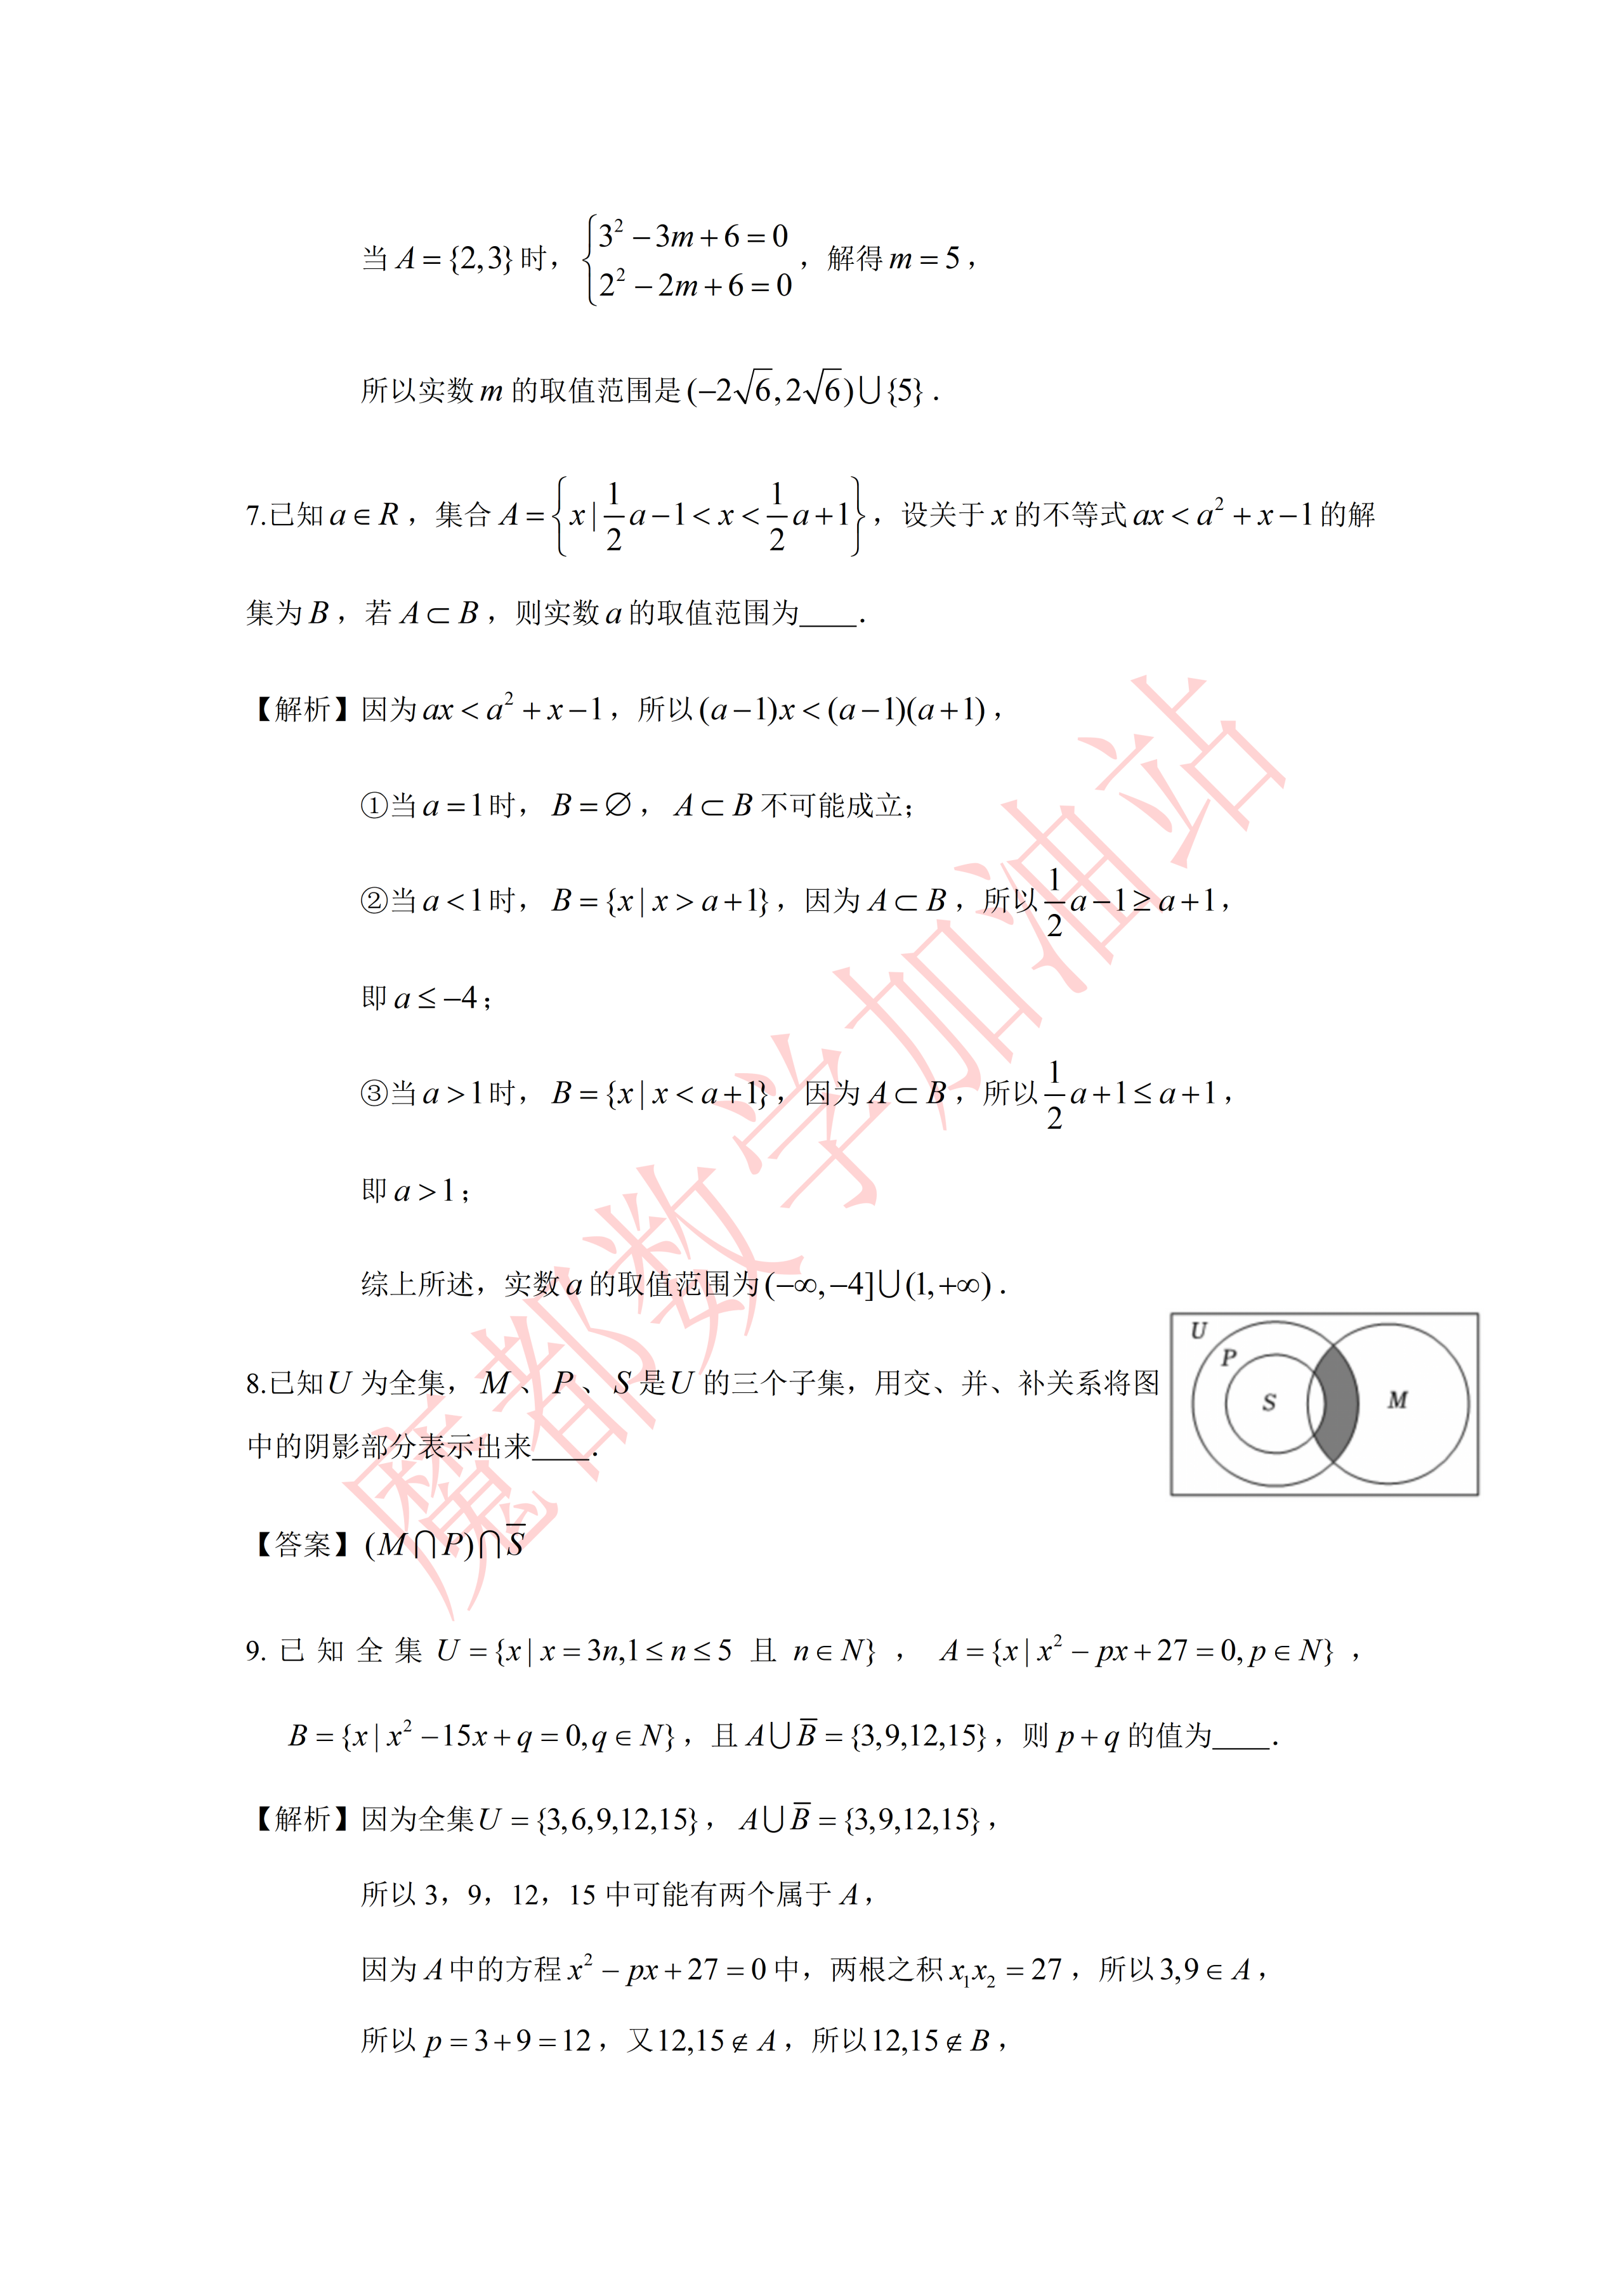
\includegraphics[width=.38\linewidth,trim=1835bp 1255bp 220bp 1565bp,clip]{../原图/高一49_华师大二附中_国庆作业1/02.png}
\end{center}

\ifanswer
\ans{$(M\cap P)\cap\overline S$}
\fi

\item 已知全集 $U=\{x\mid x=3n,1\leqslant n\leqslant5\text{ 且 }n\in\N\}$，$A=\{x\mid x^2-px+27=0,p\in\N\}$，$B=\{x\mid x^2-15x+q=0,q\in\N\}$，且 $A\cup\overline B=\{3,9,12,15\}$，则 $p+q$ 的值为\blankline[4.4em].

\ifanswer
\solbegin
\step{因为全集 $U=\{3,6,9,12,15\}$，$A\cup\overline B=\{3,9,12,15\}$，}
\step{所以 $3$、$9$、$12$、$15$ 中可能有两个属于 $A$，}
\step{因为 $A$ 中的方程 $x^2-px+27=0$ 中，两根之积 $x_1x_2=27$，所以 $3,9\in A$，}
\step{所以 $p=3+9=12$，又 $12,15\notin A$，所以 $12,15\notin B$，}
\step{因为 $B$ 中的方程 $x^2-15x+q=0$ 中，两根之和 $x_3+x_4=15$，所以 $6,9\in B$，}
\step{则 $q=6\times9=54$，所以 $p+q=66$.}
\solend
\fi

\item 已知集合 $A=\{x\mid x^2+(2a-3)x-3a=0,a\in\R,x\in\R\}$，集合 $B=\{x\mid x^2+(a-3)x+a^2-3a=0,a\in\R,x\in\R\}$，若 $A\neq B$，$A\cap B\neq\varnothing$，则 $A\cup B=$\blankline[4.4em].

\ifanswer
\solbegin
\step{设两个集合中的方程的公共解是 $b$，}
\step{由 $b^2+(2a-3)b-3a=b^2+(a-3)b+a^2-3a$，得 $ab=a^2$，}
\step{则 $a=0$ 或 $b=a$，}
\step{当 $a=0$ 时，不合题意，}
\step{当 $b=a$ 时，即两个方程的公共解为 $b=a$，}
\step{将 $b=a$ 代入方程，得 $a^2=2a$，$a=2$，}
\step{所以 $A=\{2,-3\}$，$B=\{-1,2\}$，所以 $A\cup B=\{-1,2,-3\}$.}
\solend
\fi

\item 已知一个有四个数字元素的集合 $S$，$S$ 的所有子集的元素和（空集的元素和认为是 $0$）的总和为 $16192$，则 $S$ 的元素之和等于\blankline[4.4em].

\ifanswer
\solbegin
\step{设 $S=\{a_1,a_2,a_3,a_4\}$，$S$ 的每个元素在所有子集中均出现 $2^3$ 次，}
\step{故 $(a_1+a_2+a_3+a_4)\cdot2^3=16192$，所以 $a_1+a_2+a_3+a_4=2024$，}
\step{故 $S$ 的元素之和等于 $2024$.}
\solend
\fi

\item 设 $P$ 为非空实数集满足：对任意给定的 $x,y\in P$（$x$、$y$ 可以相同），都有 $x+y\in P,x-y\in P,xy\in P$，则称 $P$ 为封闭集．关于封闭集有下列结论：

①集合 $P=\{-2,-1,0,1,2\}$ 为封闭集；

②集合 $P=\{x\mid x=2n,n\in\Z\}$ 为封闭集；

③若集合 $P_1$、$P_2$ 为封闭集，则 $P_1\cup P_2$ 为封闭集；

④若集合 $P$ 为封闭集，则一定有 $0\in P$；

⑤若集合 $P_1$、$P_2$ 为封闭集，则 $P_1\cap P_2$ 为封闭集.

其中正确结论的序号是\blankline[4.4em].

\ifanswer
\solbegin
\step{对于集合 $P=\{-2,-1,0,1,2\}$，取 $x=2$，$y=-2$，则 $x-y=2-(-2)=4\notin P$，}
\step{不满足封闭集的定义，所以①错误.}
\step{对于集合 $P=\{x\mid x=2n,n\in\Z\}$，设 $x=2n_1$，$y=2n_2$，$n_1,n_2\in\Z$.}
\step{$x+y=2n_1+2n_2=2(n_1+n_2)$，因为 $n_1+n_2\in\Z$，所以 $x+y\in P$.}
\step{$x-y=2n_1-2n_2=2(n_1-n_2)$，因为 $n_1-n_2\in\Z$，所以 $x-y\in P$.}
\step{$xy=2n_1\times2n_2=4n_1n_2=2(2n_1n_2)$，因为 $2n_1n_2\in\Z$，所以 $xy\in P$.}
\step{满足封闭集的定义，所以②正确.}
\step{令 $P_1=\{x\mid x=2n,n\in\Z\}$，$P_2=\{x\mid x=3n,n\in\Z\}$，都是封闭集.}
\step{$P_1\cup P_2$ 中，取 $x=2(x\in P_1)$，$y=3(y\in P_2)$，$x+y=5\notin P_1\cup P_2$，}
\step{不满足封闭集的定义，所以③错误.}
\step{因为对任意 $x\in P$，有 $x-x=0\in P$，}
\step{所以若集合 $P$ 为封闭集，则一定有 $0\in P$，所以④正确.}
\step{因为 $P_1$、$P_2$ 为封闭集，设 $x,y\in P_1\cap P_2$，则 $x,y\in P_1$ 且 $x,y\in P_2$.}
\step{因为 $P_1$ 是封闭集，所以 $x+y\in P_1,x-y\in P_1,xy\in P_1$.}
\step{因为 $P_2$ 是封闭集，所以 $x+y\in P_2,x-y\in P_2,xy\in P_2$.}
\step{所以 $x+y\in P_1\cap P_2,x-y\in P_1\cap P_2,xy\in P_1\cap P_2$，满足封闭集的定义，}
\step{所以⑤正确.}
\step{故正确的是②④⑤.}
\solend
\fi

\end{enumerate}

\bigsec{二、选择题}

\begin{enumerate}
\setcounter{enumi}{12}

\item 已知集合 $A=\{1,3,\sqrt m\}$，$B=\{1,m\}$，$B\subseteq A$，则 $m=$\mbox{（\quad）}

\keepwithprev
A. $0$ 或 $\sqrt3$\qquad B. $0$ 或 $3$

C. $1$ 或 $\sqrt3$\qquad D. $1$ 或 $3$

\ifanswer
\solbegin
\step{因为集合 $A=\{1,3,\sqrt m\}$，$B=\{1,m\}$，$B\subseteq A$，所以 $m=3$ 或 $m=\sqrt m$，}
\step{若 $m=3$，$A=\{1,3,\sqrt3\}$，$B=\{1,3\}$，满足 $B\subseteq A$，}
\step{若 $m=\sqrt m$，解得 $m=1$ 或 $m=0$，}
\step{①若 $m=0$，则 $A=\{1,3,0\}$，$B=\{1,0\}$，满足 $B\subseteq A$.}
\step{②若 $m=1$，则 $A$、$B$ 不满足集合中元素的互异性，舍去.}
\step{综上，$m=0$ 或 $m=3$．故选 $B$.}
\solend
\fi

\needvspace{10\baselineskip}

\item 设集合 $A$、$B$、$C$、$D$ 是全集 $X$ 的子集，$A\cap B\neq\varnothing$，$A\cap C\neq\varnothing$，则下列选项中正确的是\mbox{（\quad）}

\keepwithprev
A. 如果 $D\subset B$ 或 $D\subset C$，则 $D\cap A\neq\varnothing$

B. 如果 $D\subset A$，则 $\overline D\cap B\neq\varnothing$，$\overline D\cap C\neq\varnothing$

C. 如果 $A\subset D$，则 $\overline D\cap B=\varnothing$，$\overline D\cap C=\varnothing$

D. 上述各项都不正确

\ifanswer
\solbegin
\step{用韦恩图表示每个选项：}
\begin{center}
% 原图第 5 页解析配图（三联韦恩图）直接裁取（原卷排于选项 C、D 右侧）。
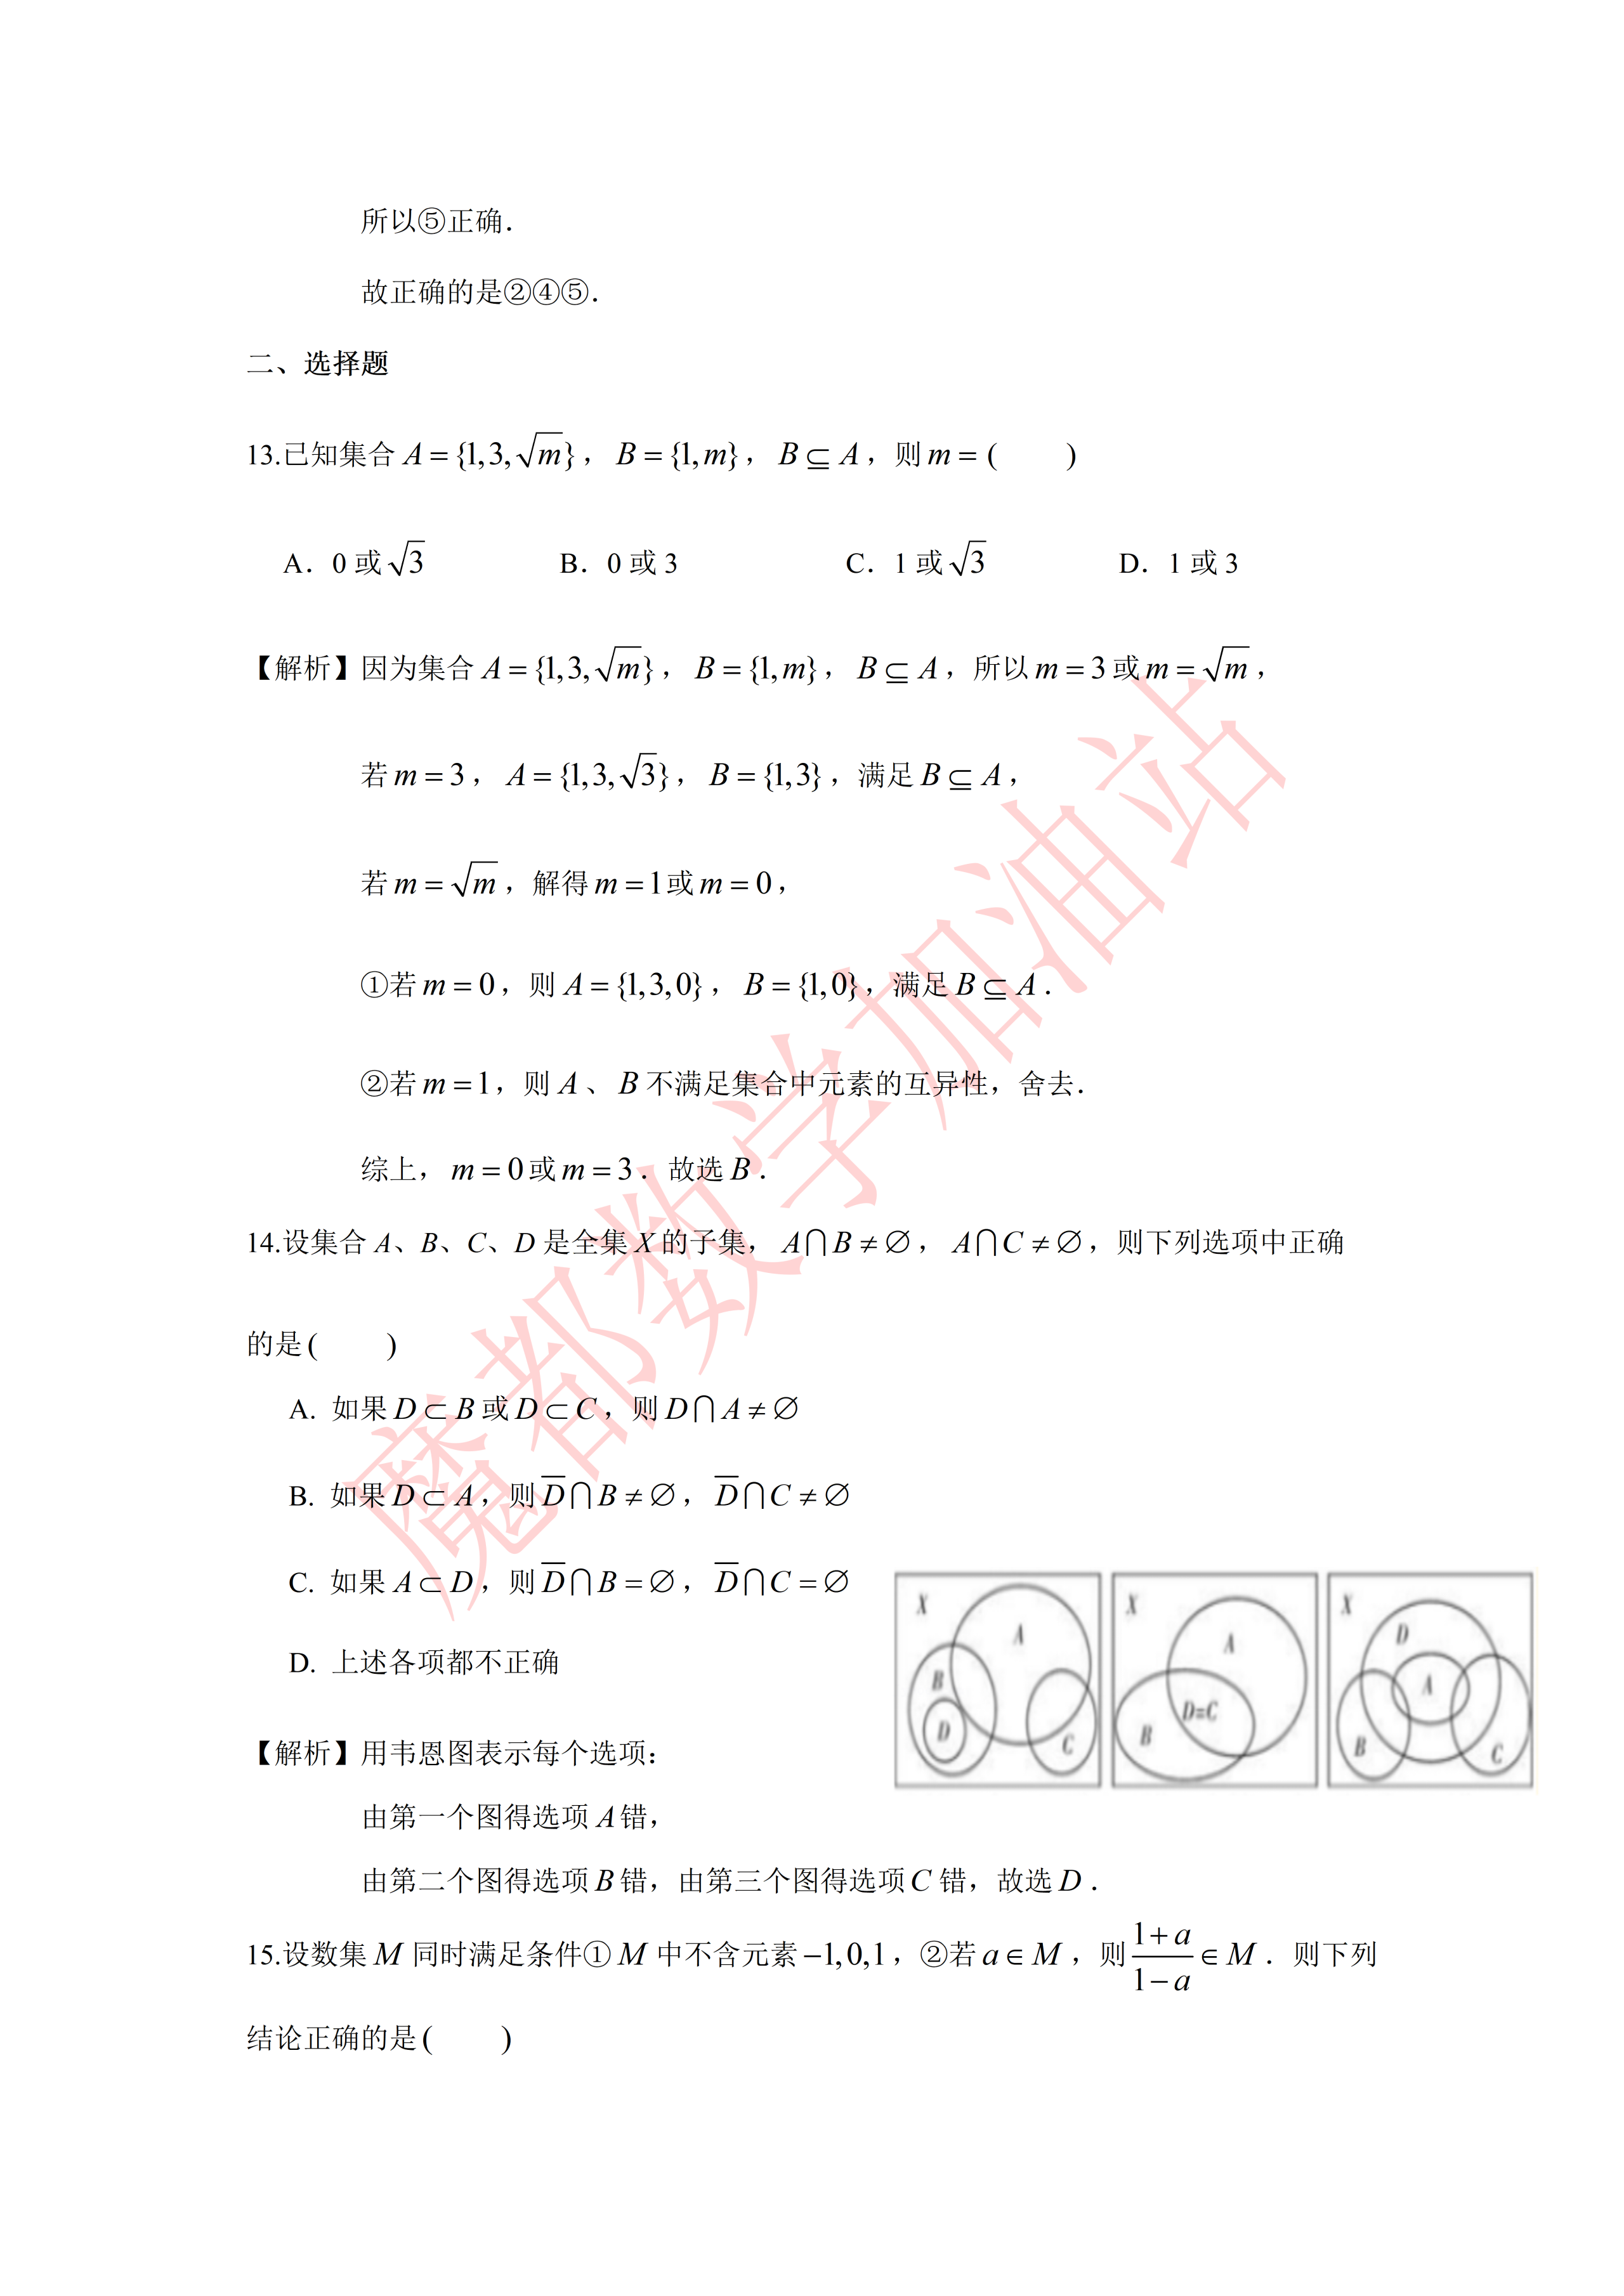
\includegraphics[width=.75\linewidth,trim=1400bp 790bp 135bp 1155bp,clip]{../原图/高一49_华师大二附中_国庆作业1/05.png}
\end{center}
\step{由第一个图得选项 $A$ 错，}
\step{由第二个图得选项 $B$ 错，由第三个图得选项 $C$ 错，故选 $D$.}
\solend
\fi

\item 设数集 $M$ 同时满足条件①$M$ 中不含元素 $-1$、$0$、$1$，②若 $a\in M$，则 $\dfrac{1+a}{1-a}\in M$．则下列结论正确的是\mbox{（\quad）}

\keepwithprev
A. 集合 $M$ 中至多有 $2$ 个元素\qquad B. 集合 $M$ 中至多有 $3$ 个元素

C. 集合 $M$ 中有且仅有 $4$ 个元素\qquad D. 集合 $M$ 中有无穷多个元素

\ifanswer
\solbegin
\step{若集合只含有一个元素，则 $\dfrac{1+a}{1-a}=a$，即 $1+a=a-a^2$，即 $-a^2=1$，不成立.}
\step{当 $a=3$ 时，$\dfrac{1+3}{1-3}=-2\in M$，所以 $\dfrac{1-2}{1+2}=-\dfrac13\in M$，所以 $\dfrac{1-\frac13}{1+\frac13}=\dfrac12\in M$，}
\step{所以 $\dfrac{1+\frac12}{1-\frac12}=3$，开始重复了，所以 $M=\left\{3,-2,-\dfrac13,\dfrac12\right\}$；}
\step{当 $a=2$ 时，$\dfrac{1+2}{1-2}=-3\in M$，所以 $\dfrac{1-3}{1+3}=-\dfrac12\in M$，所以 $\dfrac{1-\frac12}{1+\frac12}=\dfrac13\in M$，}
\step{所以 $\dfrac{1+\frac13}{1-\frac13}=2$，开始重复了，所以 $M=\left\{2,-3,-\dfrac12,-\dfrac13\right\}$，}
\step{此时也只要四个元素；}
\step{当 $a=\dfrac34\in M$，则 $7\in M$，若 $7\in M$，则 $-\dfrac43\in M$，}
\step{若 $-\dfrac43\in M$，则 $-\dfrac17\in M$，若 $-\dfrac17\in M$，有 $\dfrac34\in M$，}
\step{由归纳推理得，集合 $M$ 中有且仅有 $4$ 个元素．故选 $C$.}
\solend
\fi

\item 已知集合 $M=\{x\mid x\in\N,0<x\leqslant15\}$，$A_1$、$A_2$、$A_3$ 满足：①$A_1\cup A_2\cup A_3=M$；②每个集合都恰有 $5$ 个元素．集合 $A_i$（$i=1,2,3$）中最大元素与最小元素之和称为 $A_i$ 的特征数，记为 $X_i$（$i=1,2,3$），则 $X_1+X_2+X_3$ 的值不可能为\mbox{（\quad）}

\keepwithprev
A. $37$\qquad B. $39$\qquad C. $48$\qquad D. $57$

\ifanswer
\solbegin
\step{因为集合 $M=\{x\mid x\in\N,0<x\leqslant15\}=\{1,2,3,\cdots,15\}$，}
\step{又因为集合 $A_1$、$A_2$、$A_3$ 中，每个集合恰有 $5$ 个元素，}
\step{且 $A_1\cup A_2\cup A_3=M$ 有 $15$ 个元素，所以集合 $A_1$、$A_2$、$A_3$ 中没有重复元素，}
\step{因为 $1$ 是集合 $M$ 中数值最小的元素，$15$ 是集合 $M$ 中数值最大的元素，}
\step{所以在 $A_i$ 的特征数构成中，必有 $1$ 和 $15$，不妨设 $1\in A_1$，$15\in A_1$，}
\step{要使 $X_1+X_2+X_3$ 最大，则应该在集合 $A_1$ 中首先放置数值较小的元素，}
\step{即 $A_1=\{1,2,3,4,15\}$，所以 $5$ 与 $14$ 是剩下元素中数值最小或最大的元素，}
\step{同理，不妨设 $5\in A_2$，$14\in A_2$，接着在 $A_2$ 中再次放置数值较小的元素，}
\step{即 $A_2=\{5,6,7,8,14\}$，则 $A_3=\{9,10,11,12,13\}$，}
\step{此时 $X_1+X_2+X_3$ 有最大值为 $1+15+5+14+9+13=57$，}
\step{即 $X_1+X_2+X_3\leqslant57$；}
\step{要使 $X_1+X_2+X_3$ 最小，则在集合 $A_1$ 中首先放置数值较大的元素，}
\step{即 $A_1=\{1,12,13,14,15\}$，所以 $2$ 与 $11$ 是剩下元素中数值最小或最大的元素，}
\step{同理，不妨设 $2\in A_2$，$11\in A_2$，接着在 $A_2$ 中再次放置数值较大的元素，}
\step{即 $A_2=\{2,8,9,10,11\}$，则 $A_3=\{3,4,5,6,7\}$，}
\step{此时 $X_1+X_2+X_3$ 有最小值为 $1+15+2+11+3+7=39$，}
\step{即 $X_1+X_2+X_3\geqslant39$，}
\step{综上，$39\leqslant X_1+X_2+X_3\leqslant57$，故选 $A$.}
\solend
\fi

\end{enumerate}

\bigsec{三、解答题}

\begin{enumerate}
\setcounter{enumi}{16}

\item 已知全集为 $\R$，集合 $A=\{x\mid y=\sqrt{(2+x)(4-x)}\}$，$B=\{x\mid-1<x<m+1\}$.

\begin{enumerate}[label=(\arabic*)]
\item 若 $m=4$，求 $A\cup B$、$\overline A\cap B$；
\item 若 $B\subseteq A$，求实数 $m$ 的取值范围.
\end{enumerate}

\ifanswer
\solbegin
\stepm{(1)}{集合 $A=\{x\mid y=\sqrt{(2+x)(4-x)}\}=\{x\mid-2\leqslant x\leqslant4\}$，}
\step{当 $m=4$ 时，$B=\{x\mid-1<x<5\}$.}
\step{所以 $A\cup B=[-2,5)$，$\overline A=\{x\mid x<-2\text{ 或 }x>4\}$，$\overline A\cap B=(4,5)$.}
\stepm{(2)}{因为 $B\subseteq A$，}
% 原卷如此，照录未改（第 17 题(2)解析两处"当 C=∅／当 C≠∅"应为 B，本卷并无集合 C）
\step{当 $C=\varnothing$ 时，$m\leqslant-2$，$B\subseteq A$ 成立；}
\step{当 $C\neq\varnothing$ 时，$m>-2$，$-1<m+1\leqslant4$，解得 $-2<m\leqslant3$，}
\step{综上，$m\leqslant3$，所以实数 $m$ 的取值范围是 $(-\infty,3]$.}
\solend
\fi

\ansspace[6]

\item 用反证法证明：若 $a$、$b$、$c\in\R$，且 $x=a^2-2b+1$，$y=b^2-2c+1$，$z=c^2-2a+1$，则 $x$、$y$、$z$ 中至少有一个不小于 $0$.

\ifanswer
\solbegin
\step{假设 $x$、$y$、$z$ 均小于 $0$，即 $x=a^2-2b+1<0$①，$y=b^2-2c+1<0$②，}
\step{$z=c^2-2a+1<0$③，①$+$②$+$③得 $x+y+z=(a-1)^2+(b-1)^2+(c-1)^2<0$，}
\step{这与 $(a-1)^2+(b-1)^2+(c-1)^2\geqslant0$ 矛盾，则假设不成立，}
\step{所以 $x$、$y$、$z$ 中至少有一个不小于 $0$，得证.}
\solend
\fi

\ansspace[5]

\item 已知全集为 $\R$，实数 $a$、$b$ 满足 $a\neq b$，集合 $M=\{x\mid x^2-3x-4\leqslant0\}$，集合 $A=\{x\mid(x+a)(x+b)>0\}$，集合 $B=\{x\mid x^2+(a-2)x-2a>0\}$.

\begin{enumerate}[label=(\arabic*)]
\item 若 $\overline A=M$，求 $a$、$b$ 的值；
\item 若 $a>b>-1$，求 $A\cap B$；
\item 若 $a^2+a\in\overline B$，求 $a$ 的取值范围.
\end{enumerate}

\ifanswer
\solbegin
\stepm{(1)}{$M=\{x\mid x^2-3x-4\leqslant0\}=\{x\mid-1\leqslant x\leqslant4\}$，$A=\{x\mid(x+a)(x+b)\leqslant0\}$，}
\step{因为 $\overline A=M$，所以 $a=1$，$b=-4$ 或 $a=-4$，$b=1$.}
\stepm{(2)}{因为 $a>b>-1$，所以 $-a<-b<1$，所以 $A=\{x\mid x<-a\text{ 或 }x>-b\}$，}
\step{因为 $B=\{x\mid x^2+(a-2)x-2a>0\}=\{x\mid x<-a\text{ 或 }x>2\}$，}
\step{所以 $A\cap B=\{x\mid x<-a\text{ 或 }x>2\}$，}
\stepm{(3)}{$\overline B=\{x\mid(x-2)(x+a)\leqslant0\}$，}
% 原卷如此，照录未改（第 19 题(3)此处"a(a-1)((a-2)^2≤0"括号不配对；且由左式展开应为
% a(a-1)(a+2)^2≤0，与下句"解得 a=2 …[0,1]∪{2}"按 (a-2)^2 方自洽，见文件头清单第 2 条）
\step{由 $a^2+a\in\overline B$，得 $(a^2+a-2)(a^2+2a)\leqslant0\Leftrightarrow a(a-1)((a-2)^2\leqslant0$，}
\step{解得 $a=2$ 或 $0\leqslant a\leqslant1$，故 $a$ 的取值范围是 $[0,1]\cup\{2\}$.}
\solend
\fi

\ansspace[7]

\item 设数集 $A$ 由实数构成，若 $x\in A$（$x\neq1$ 且 $x\neq0$），则 $\dfrac{1}{1-x}\in A$.

\begin{enumerate}[label=(\arabic*)]
\item 若 $2\in A$，则 $A$ 中至少还有几个元素；
\item 集合 $A$ 是否为双元素集合？请说明理由；
\item 若 $A$ 中元素个数不超过 $8$ 个，所有元素的和为 $\dfrac{14}{3}$，且 $A$ 中有一个元素的平方等于所有元素的积，求集合 $A$.
\end{enumerate}

\ifanswer
\solbegin
\stepm{(1)}{若 $x\in A$，则 $\dfrac{1}{1-x}\in A$，又 $2\in A$，所以 $\dfrac{1}{1-2}=-1\in A$，}
\step{所以 $\dfrac{1}{1-(-1)}=\dfrac12\in A$，所以 $\dfrac{1}{1-\frac12}=2\in A$，}
% 原卷如此，照录未改（第 20 题(1)解析末句"2 个几个元素"衍一"几个"）
\step{所以 $A$ 中至少还有 $2$ 个几个元素；}
\stepm{(2)}{若 $x\in A$（$x\neq1$ 且 $x\neq0$），则 $\dfrac{1}{1-x}\in A$，}
\step{则 $\dfrac{1}{1-\frac{1}{1-x}}=\dfrac{1-x}{-x}\in A$，则 $\dfrac{1}{1-\frac{1-x}{-x}}=x\in A$}
\step{若 $A$ 为双元素集，则 $x=\dfrac{1}{1-x}$ 或 $x=\dfrac{1-x}{-x}$ 或 $\dfrac{1}{1-x}=\dfrac{1-x}{-x}$，均无解，}
\step{所以 $A$ 不可能为双元素集；}
\stepm{(3)}{由 $x\in A$，$\dfrac{1}{1-x}\in A$，得 $\dfrac{1}{1-\frac{1}{1-x}}=\dfrac{x-1}{x}\in A$，得 $\dfrac{1}{1-\frac{x-1}{x}}=x\in A$，}
\step{所以 $\left\{x,\dfrac{1}{1-x},\dfrac{x-1}{x}\right\}\subseteq A$，而 $x\cdot\dfrac{1}{1-x}\cdot\dfrac{x-1}{x}=-1$，}
\step{$A$ 中元素个数为 $3$ 的倍数，则 $A$ 中元素只有 $6$ 个，}
\step{因为 $A$ 中有一个元素的平方等于所有元素的积，}
\step{不妨设 $x^2=1$，解得 $x=-1$ 或 $x=1$（舍），则 $-1$、$\dfrac12$、$2\in A$，}
\step{所以 $-1+\dfrac12+2+m+\dfrac{1}{1-m}+\dfrac{m-1}{m}=\dfrac{14}{3}$，解得 $m=-\dfrac12$ 或 $m=3$ 或 $m=\dfrac23$，}
\step{所以 $A=\left\{\dfrac12,2,-1,-\dfrac12,3,\dfrac23\right\}$.}
\solend
\fi

\ansspace[9]

% 原卷如此，照录未改（第 21 题题干"21.求已知集合"之"求"字疑衍；"任意两个元素 a_i a_j"
% 疑脱逗号；"|a_i-a_j|≥1/30 则称"之前疑脱标点，见文件头清单第 4 条）
\item 求已知集合 $M=\left\{\dfrac{1}{k}\middle|1\leqslant k\leqslant100\text{ 且 }k\in\N^{*}\right\}$，$A=\{a_1,a_2,\cdots,a_n\}$，其中 $n\in\N^{*}$，且 $n\geqslant2$．若 $A\subseteq\N$，且对集合 $A$ 中的任意两个元素 $a_ia_j$，$i\neq j$ 都有 $|a_i-a_j|\geqslant\dfrac{1}{30}$ 则称集合 $A$ 有性质 $P$.

\begin{enumerate}[label=(\arabic*)]
\item 判断集合 $\left\{\dfrac13,\dfrac14,\dfrac15,\dfrac16,\dfrac17\right\}$ 是否具有性质 $P$；
\item 若集合 $A=\{a_1,a_2,\cdots,a_n\}$ 具有性质 $P$.

①求证：$a_i-a_j$ 的最大值大于等于 $\dfrac{n-1}{30}$；

②求 $A$ 的元素个数 $n$ 的最大值.
\end{enumerate}

\ifanswer
\solbegin
\stepm{(1)}{集合为 $\left\{\dfrac13,\dfrac14,\dfrac15,\dfrac16,\dfrac17\right\}$，又 $\dfrac16-\dfrac17=\dfrac{1}{42}<\dfrac{1}{30}$，所以该集合不具有性质 $P$；}
\stepm{(2)}{①因为集合 $A=\{a_1,a_2,\cdots,a_n\}$ 具有性质 $P$，}
\step{不妨设 $a_1<a_2<a_3<\cdots<a_n$，则 $a_i-a_j\geqslant\dfrac{1}{30}$（$i>j$），}
\step{所以 $a_n-a_1=(a_n-a_{n-1})+(a_{n-1}-a_{n-2})+\cdots+(a_2-a_1)\geqslant\dfrac{n-1}{30}$，}
\step{故 $a_i-a_j$ 的最大值大于等于 $\dfrac{n-1}{30}$；}
% 原卷如此，照录未改（第 21 题(2)②首行"a_2-a_1≥(n-1)/30"：由①同款推理只能得
% a_2-a_1≥1/30，见文件头清单第 5 条）
\step{②$A=\{a_1,a_2,\cdots,a_n\}$，不妨设 $a_1<a_2<a_3<\cdots<a_n$，}
\step{要使 $A$ 的元素个数 $n$ 最大，}
\step{则 $A$ 中的元素满足 $a_n=\dfrac{1}{k}$，$a_{n-1}=\dfrac{1}{k+1}$，$\cdots$，$a_1=\dfrac{1}{k+n-1}$（$k\in\N^{*}$），}
\step{又由①得 $a_2-a_1=\dfrac{1}{k+n-2}-\dfrac{1}{k+n-1}\geqslant\dfrac{n-1}{30}$，}
\step{所以 $(k+n-2)(k+n-1)\leqslant30$，又 $a_n-a_{n-1}=\dfrac{1}{k}-\dfrac{1}{k+1}\geqslant\dfrac{1}{30}$，}
\step{所以 $k(k+1)\leqslant30$，所以 $1\leqslant k\leqslant5$（$k\in\N^{*}$），}
\step{当 $k=5$ 时，由 $(k+n-2)(k+n-1)\leqslant30$，解得 $n\leqslant2$，$n\in\N^{*}$；}
\step{当 $k=4$ 时，由 $(k+n-2)(k+n-1)\leqslant30$，解得 $n\leqslant3$，$n\in\N^{*}$；}
\step{当 $k=3$ 时，由 $(k+n-2)(k+n-1)\leqslant30$，解得 $n\leqslant4$，$n\in\N^{*}$；}
\step{当 $k=2$ 时，由 $(k+n-2)(k+n-1)\leqslant30$，解得 $n\leqslant5$，$n\in\N^{*}$；}
\step{当 $k=1$ 时，由 $(k+n-2)(k+n-1)\leqslant30$，解得 $n\leqslant6$，$n\in\N^{*}$.}
\step{故 $A$ 的元素个数 $n$ 的最大值为 $6$，此时集合 $A=\left\{1,\dfrac12,\dfrac13,\cdots,\dfrac16\right\}$.}
\solend
\fi

\ansspace*[10]

\end{enumerate}

\end{document}
"
%
% 原始材料：微信公众号"魔都数学加油站"文章，作者破晓，连载"27学年高一49"；
% 原文标题"27学年高一49——2026-2027年上海市华师大二附中高一上国庆作业1集合与逻辑、
% 等式与不等式的性质"；页面用 JS 渲染，未见明确发布日期（页内时间戳 ≈ 2026-10-05 21:37）；
% 原文链接：https://mp.weixin.qq.com/s/XxZTOBVQslK5cZm2_BbhOg。
% 正文为 11 张 PNG 页：第 01、03、04、06、07、08、09 页 4762×6735，
% 第 02、05、10、11 页 2560×3620，均按页序读取；粉色斜排"魔都数学加油站"为卷面水印，
% 与公众号页脚一并未录入。全卷 11 页均为试卷页，无二维码/宣传页。
%
% 题号与分节：原文自第 3 题起编，填空题 3—12、选择题 13—16、解答题 17—21，共 19 题。
% 讲评版：原卷每题下直接印【答案】或【解析】——只印【答案】的 3 题（第 3、5、8 题），
% 其余 16 题均只印【解析】；解析行数已逐题按印刷行照录（一条 \step＝原卷一个印刷行）。
%
% 卷首标题：照卷面印作"2026-2027 年华师大二附中高一上国庆作业 1"（公众号标题中的"上海市"
% 卷面没有，本稿照卷面），年份区间按全稿惯例排 en dash；副标题照卷面自印的
% "集合与逻辑单元综合检测"（原卷页首标题行下方即印此行，故不另按模块口径拟名）。
% 副标题依据：全卷 19 题均为集合与常用逻辑用语内容——集合类 15 题（6—17、19—21 中除
% 反证法题外），逻辑/命题类 3 题（第 3 题否定形式、第 4 题充要条件、第 5 题反证法假设），
% 反证法证明 1 题（第 18 题）；全卷无不等式求解题，公众号标题中"等式与不等式的性质"
% 与卷面实际内容不符。
%
% 与原卷的排版差异：
%   ① 原文从第 3 题起，填空题为 3—12、选择题为 13—16、解答题为 17—21，本稿保留原题号；
%   ② 原卷每题下直接印【答案】/【解析】，本稿按全稿惯例置于答案版；只印【解析】的题
%      不另提 \ans{}（照 高一36 口径），只印【答案】的题仅给 \ans{}；
%   ③ 原卷第 8 题韦恩图排在题干右侧、第 14 题三联韦恩图排在选项（C、D）右侧，
%      本稿分别移至题干下方、解析首步之后居中排，均直接裁取原图页（02.png、05.png）；
%   ④ 数集记号原卷排作斜体/加粗 R、N、Z，本稿统一为 \R、\N、\Z、\N^*；
%      填空横线按全稿惯例排为 \blankline[4.4em]。
%
% 原卷笔误/存疑清单（均照录未改，正文中该处有 % 注）：
%   1. 第 17 题(2)解析两处"当 C=∅／当 C≠∅"应为 B（本卷并无集合 C）；
%   2. 第 19 题(3)解析"a(a-1)((a-2)^2≤0"括号不配对（多一枚左括号）；且由
%      (a^2+a-2)(a^2+2a)≤0 展开应为 a(a-1)(a+2)^2≤0，与原卷结论"解得 a=2 …
%      [0,1]∪{2}"恰按 (a-2)^2 自洽——因式分解与原式不符，结论按 (a-2)^2 自洽，均照录；
%   3. 第 20 题(1)解析末句"至少还有 2 个几个元素"衍一"几个"；
%   4. 第 21 题题干"21.求已知集合"之"求"字疑衍；"任意两个元素 a_i a_j"疑脱逗号；
%      "≥1/30 则称"之前疑脱标点；
%   5. 第 21 题(2)②解析"a_2-a_1≥(n-1)/30"：由①同款推理只能得 a_2-a_1≥1/30，
%      原卷如此，照录未改（后续 (k+n-2)(k+n-1)≤30 即按该行推得）。
%
\documentclass[a4paper,11pt]{article}
\usepackage{common}

\begin{document}

\examtitlest[3]{2026--2027 年华师大二附中高一上国庆作业 1}{集合与逻辑单元综合检测}

\bigsec{一、填空题}

\begin{enumerate}
\setcounter{enumi}{2}

\item “若 $x^2-x-2\leqslant0$，则 $-1\leqslant x\leqslant2$”的否定形式为\blankline[4.4em].

\ifanswer
\ans{若 $x^2-x-2>0$，则 $x<-1$ 或 $x>2$}
\fi

\item 已知 $p:|x-3|<5$，$q:1-a<x<2a-3$，且 $p$ 是 $q$ 的充分非必要条件，则实数 $a$ 的取值范围是\blankline[4.4em].

\ifanswer
\solbegin
\step{由 $|x-3|<5$ 得 $-2<x<8$，}
\step{又 $p$ 是 $q$ 的充分不必要条件，所以 $(-2,8)\subset(1-a,2a-3)$，}
\step{即 $\begin{cases}-2\geqslant1-a\\ 8\leqslant2a-3\\ (2a-3)-(1-a)\neq8-(-2)\end{cases}$，解得 $a\geqslant\dfrac{11}{2}$，实数 $a$ 的取值范围是 $\left[\dfrac{11}{2},+\infty\right)$.}
\solend
\fi

\item 用反证法证明命题“设 $a$、$b\in\R$，则方程 $a_1x^2+b_1x+c_1=0$ 与 $a_2x^2+b_2x+c_2=0$ 至少有一个实根”时要做的假设是\blankline[4.4em].

\ifanswer
\ans{假设 $a$、$b\in\R$，方程 $a_1x^2+b_1x+c_1=0$ 与 $a_2x^2+b_2x+c_2=0$ 都没有实根}
\fi

\item 设集合 $A=\{x\mid x^2-mx+6=0,x\in\R\}$，且 $A\cap\{2,3\}=A$，则实数 $m$ 的取值范围是\blankline[4.4em].

\ifanswer
\solbegin
\step{由 $A\cap\{2,3\}=A$，得 $A\subseteq\{2,3\}$，}
\step{当 $A=\varnothing$ 时，$\Delta=m^2-24<0$，解得 $-2\sqrt6<m<2\sqrt6$；}
\step{当 $A=\{2\}$ 时，$\begin{cases}2^2-2m+6=0\\ \Delta=m^2-24=0\end{cases}$，无解；}
\step{当 $A=\{3\}$ 时，$\begin{cases}3^2-3m+6=0\\ \Delta=m^2-24=0\end{cases}$，无解；}
\step{当 $A=\{2,3\}$ 时，$\begin{cases}3^2-3m+6=0\\ 2^2-2m+6=0\end{cases}$，解得 $m=5$，}
\step{所以实数 $m$ 的取值范围是 $(-2\sqrt6,2\sqrt6)\cup\{5\}$.}
\solend
\fi

\item 已知 $a\in\R$，集合 $A=\left\{x\middle|\dfrac12a-1<x<\dfrac12a+1\right\}$，设关于 $x$ 的不等式 $ax<a^2+x-1$ 的解集为 $B$，若 $A\subset B$，则实数 $a$ 的取值范围为\blankline[4.4em].

\ifanswer
\solbegin
\step{因为 $ax<a^2+x-1$，所以 $(a-1)x<(a-1)(a+1)$，}
\step{①当 $a=1$ 时，$B=\varnothing$，$A\subset B$ 不可能成立；}
\step{②当 $a<1$ 时，$B=\{x\mid x>a+1\}$，因为 $A\subset B$，所以 $\dfrac12a-1\geqslant a+1$，}
\step{即 $a\leqslant-4$；}
\step{③当 $a>1$ 时，$B=\{x\mid x<a+1\}$，因为 $A\subset B$，所以 $\dfrac12a+1\leqslant a+1$，}
\step{即 $a>1$；}
\step{综上所述，实数 $a$ 的取值范围为 $(-\infty,-4]\cup(1,+\infty)$.}
\solend
\fi

\needvspace{8\baselineskip}

\item 已知 $U$ 为全集，$M$、$P$、$S$ 是 $U$ 的三个子集，用交、并、补关系将图中的阴影部分表示出来\blankline[4.4em].

\begin{center}
% 原图第 2 页题旁韦恩图直接裁取（原卷排于题干右侧）。
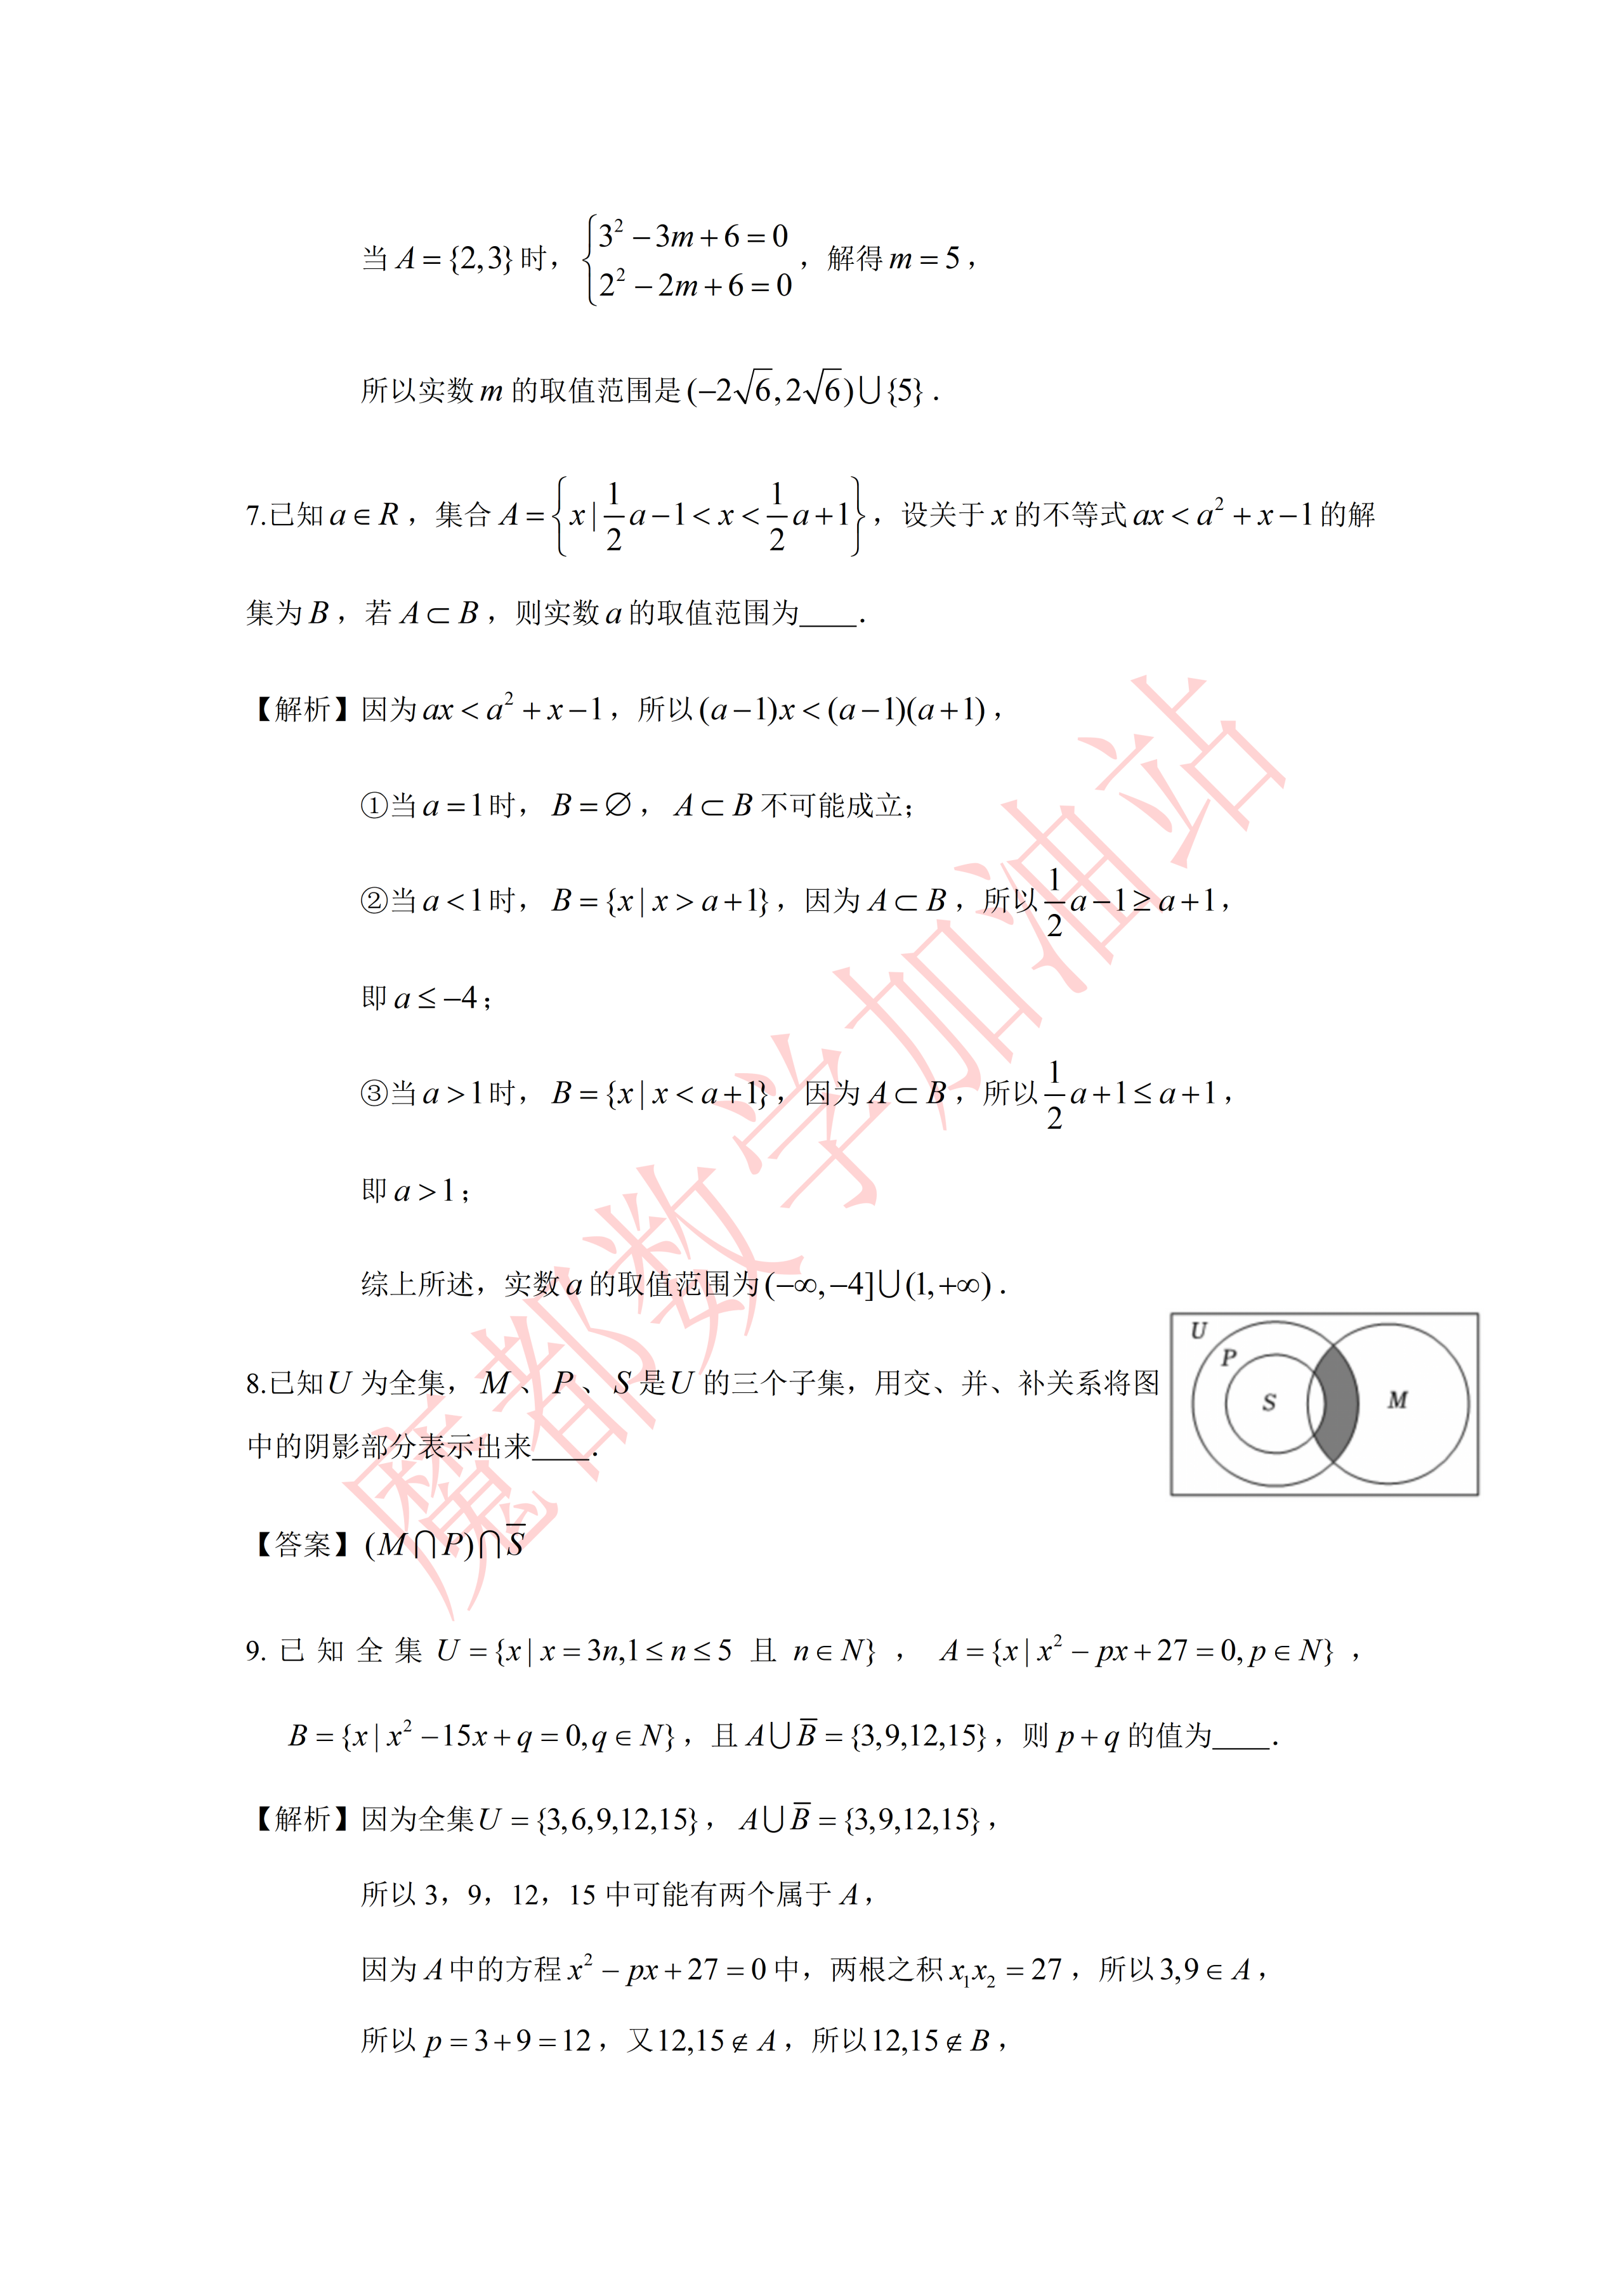
\includegraphics[width=.38\linewidth,trim=1835bp 1255bp 220bp 1565bp,clip]{../原图/高一49_华师大二附中_国庆作业1/02.png}
\end{center}

\ifanswer
\ans{$(M\cap P)\cap\overline S$}
\fi

\item 已知全集 $U=\{x\mid x=3n,1\leqslant n\leqslant5\text{ 且 }n\in\N\}$，$A=\{x\mid x^2-px+27=0,p\in\N\}$，$B=\{x\mid x^2-15x+q=0,q\in\N\}$，且 $A\cup\overline B=\{3,9,12,15\}$，则 $p+q$ 的值为\blankline[4.4em].

\ifanswer
\solbegin
\step{因为全集 $U=\{3,6,9,12,15\}$，$A\cup\overline B=\{3,9,12,15\}$，}
\step{所以 $3$、$9$、$12$、$15$ 中可能有两个属于 $A$，}
\step{因为 $A$ 中的方程 $x^2-px+27=0$ 中，两根之积 $x_1x_2=27$，所以 $3,9\in A$，}
\step{所以 $p=3+9=12$，又 $12,15\notin A$，所以 $12,15\notin B$，}
\step{因为 $B$ 中的方程 $x^2-15x+q=0$ 中，两根之和 $x_3+x_4=15$，所以 $6,9\in B$，}
\step{则 $q=6\times9=54$，所以 $p+q=66$.}
\solend
\fi

\item 已知集合 $A=\{x\mid x^2+(2a-3)x-3a=0,a\in\R,x\in\R\}$，集合 $B=\{x\mid x^2+(a-3)x+a^2-3a=0,a\in\R,x\in\R\}$，若 $A\neq B$，$A\cap B\neq\varnothing$，则 $A\cup B=$\blankline[4.4em].

\ifanswer
\solbegin
\step{设两个集合中的方程的公共解是 $b$，}
\step{由 $b^2+(2a-3)b-3a=b^2+(a-3)b+a^2-3a$，得 $ab=a^2$，}
\step{则 $a=0$ 或 $b=a$，}
\step{当 $a=0$ 时，不合题意，}
\step{当 $b=a$ 时，即两个方程的公共解为 $b=a$，}
\step{将 $b=a$ 代入方程，得 $a^2=2a$，$a=2$，}
\step{所以 $A=\{2,-3\}$，$B=\{-1,2\}$，所以 $A\cup B=\{-1,2,-3\}$.}
\solend
\fi

\item 已知一个有四个数字元素的集合 $S$，$S$ 的所有子集的元素和（空集的元素和认为是 $0$）的总和为 $16192$，则 $S$ 的元素之和等于\blankline[4.4em].

\ifanswer
\solbegin
\step{设 $S=\{a_1,a_2,a_3,a_4\}$，$S$ 的每个元素在所有子集中均出现 $2^3$ 次，}
\step{故 $(a_1+a_2+a_3+a_4)\cdot2^3=16192$，所以 $a_1+a_2+a_3+a_4=2024$，}
\step{故 $S$ 的元素之和等于 $2024$.}
\solend
\fi

\item 设 $P$ 为非空实数集满足：对任意给定的 $x,y\in P$（$x$、$y$ 可以相同），都有 $x+y\in P,x-y\in P,xy\in P$，则称 $P$ 为封闭集．关于封闭集有下列结论：

①集合 $P=\{-2,-1,0,1,2\}$ 为封闭集；

②集合 $P=\{x\mid x=2n,n\in\Z\}$ 为封闭集；

③若集合 $P_1$、$P_2$ 为封闭集，则 $P_1\cup P_2$ 为封闭集；

④若集合 $P$ 为封闭集，则一定有 $0\in P$；

⑤若集合 $P_1$、$P_2$ 为封闭集，则 $P_1\cap P_2$ 为封闭集.

其中正确结论的序号是\blankline[4.4em].

\ifanswer
\solbegin
\step{对于集合 $P=\{-2,-1,0,1,2\}$，取 $x=2$，$y=-2$，则 $x-y=2-(-2)=4\notin P$，}
\step{不满足封闭集的定义，所以①错误.}
\step{对于集合 $P=\{x\mid x=2n,n\in\Z\}$，设 $x=2n_1$，$y=2n_2$，$n_1,n_2\in\Z$.}
\step{$x+y=2n_1+2n_2=2(n_1+n_2)$，因为 $n_1+n_2\in\Z$，所以 $x+y\in P$.}
\step{$x-y=2n_1-2n_2=2(n_1-n_2)$，因为 $n_1-n_2\in\Z$，所以 $x-y\in P$.}
\step{$xy=2n_1\times2n_2=4n_1n_2=2(2n_1n_2)$，因为 $2n_1n_2\in\Z$，所以 $xy\in P$.}
\step{满足封闭集的定义，所以②正确.}
\step{令 $P_1=\{x\mid x=2n,n\in\Z\}$，$P_2=\{x\mid x=3n,n\in\Z\}$，都是封闭集.}
\step{$P_1\cup P_2$ 中，取 $x=2(x\in P_1)$，$y=3(y\in P_2)$，$x+y=5\notin P_1\cup P_2$，}
\step{不满足封闭集的定义，所以③错误.}
\step{因为对任意 $x\in P$，有 $x-x=0\in P$，}
\step{所以若集合 $P$ 为封闭集，则一定有 $0\in P$，所以④正确.}
\step{因为 $P_1$、$P_2$ 为封闭集，设 $x,y\in P_1\cap P_2$，则 $x,y\in P_1$ 且 $x,y\in P_2$.}
\step{因为 $P_1$ 是封闭集，所以 $x+y\in P_1,x-y\in P_1,xy\in P_1$.}
\step{因为 $P_2$ 是封闭集，所以 $x+y\in P_2,x-y\in P_2,xy\in P_2$.}
\step{所以 $x+y\in P_1\cap P_2,x-y\in P_1\cap P_2,xy\in P_1\cap P_2$，满足封闭集的定义，}
\step{所以⑤正确.}
\step{故正确的是②④⑤.}
\solend
\fi

\end{enumerate}

\bigsec{二、选择题}

\begin{enumerate}
\setcounter{enumi}{12}

\item 已知集合 $A=\{1,3,\sqrt m\}$，$B=\{1,m\}$，$B\subseteq A$，则 $m=$\mbox{（\quad）}

\keepwithprev
A. $0$ 或 $\sqrt3$\qquad B. $0$ 或 $3$

C. $1$ 或 $\sqrt3$\qquad D. $1$ 或 $3$

\ifanswer
\solbegin
\step{因为集合 $A=\{1,3,\sqrt m\}$，$B=\{1,m\}$，$B\subseteq A$，所以 $m=3$ 或 $m=\sqrt m$，}
\step{若 $m=3$，$A=\{1,3,\sqrt3\}$，$B=\{1,3\}$，满足 $B\subseteq A$，}
\step{若 $m=\sqrt m$，解得 $m=1$ 或 $m=0$，}
\step{①若 $m=0$，则 $A=\{1,3,0\}$，$B=\{1,0\}$，满足 $B\subseteq A$.}
\step{②若 $m=1$，则 $A$、$B$ 不满足集合中元素的互异性，舍去.}
\step{综上，$m=0$ 或 $m=3$．故选 $B$.}
\solend
\fi

\needvspace{10\baselineskip}

\item 设集合 $A$、$B$、$C$、$D$ 是全集 $X$ 的子集，$A\cap B\neq\varnothing$，$A\cap C\neq\varnothing$，则下列选项中正确的是\mbox{（\quad）}

\keepwithprev
A. 如果 $D\subset B$ 或 $D\subset C$，则 $D\cap A\neq\varnothing$

B. 如果 $D\subset A$，则 $\overline D\cap B\neq\varnothing$，$\overline D\cap C\neq\varnothing$

C. 如果 $A\subset D$，则 $\overline D\cap B=\varnothing$，$\overline D\cap C=\varnothing$

D. 上述各项都不正确

\ifanswer
\solbegin
\step{用韦恩图表示每个选项：}
\begin{center}
% 原图第 5 页解析配图（三联韦恩图）直接裁取（原卷排于选项 C、D 右侧）。
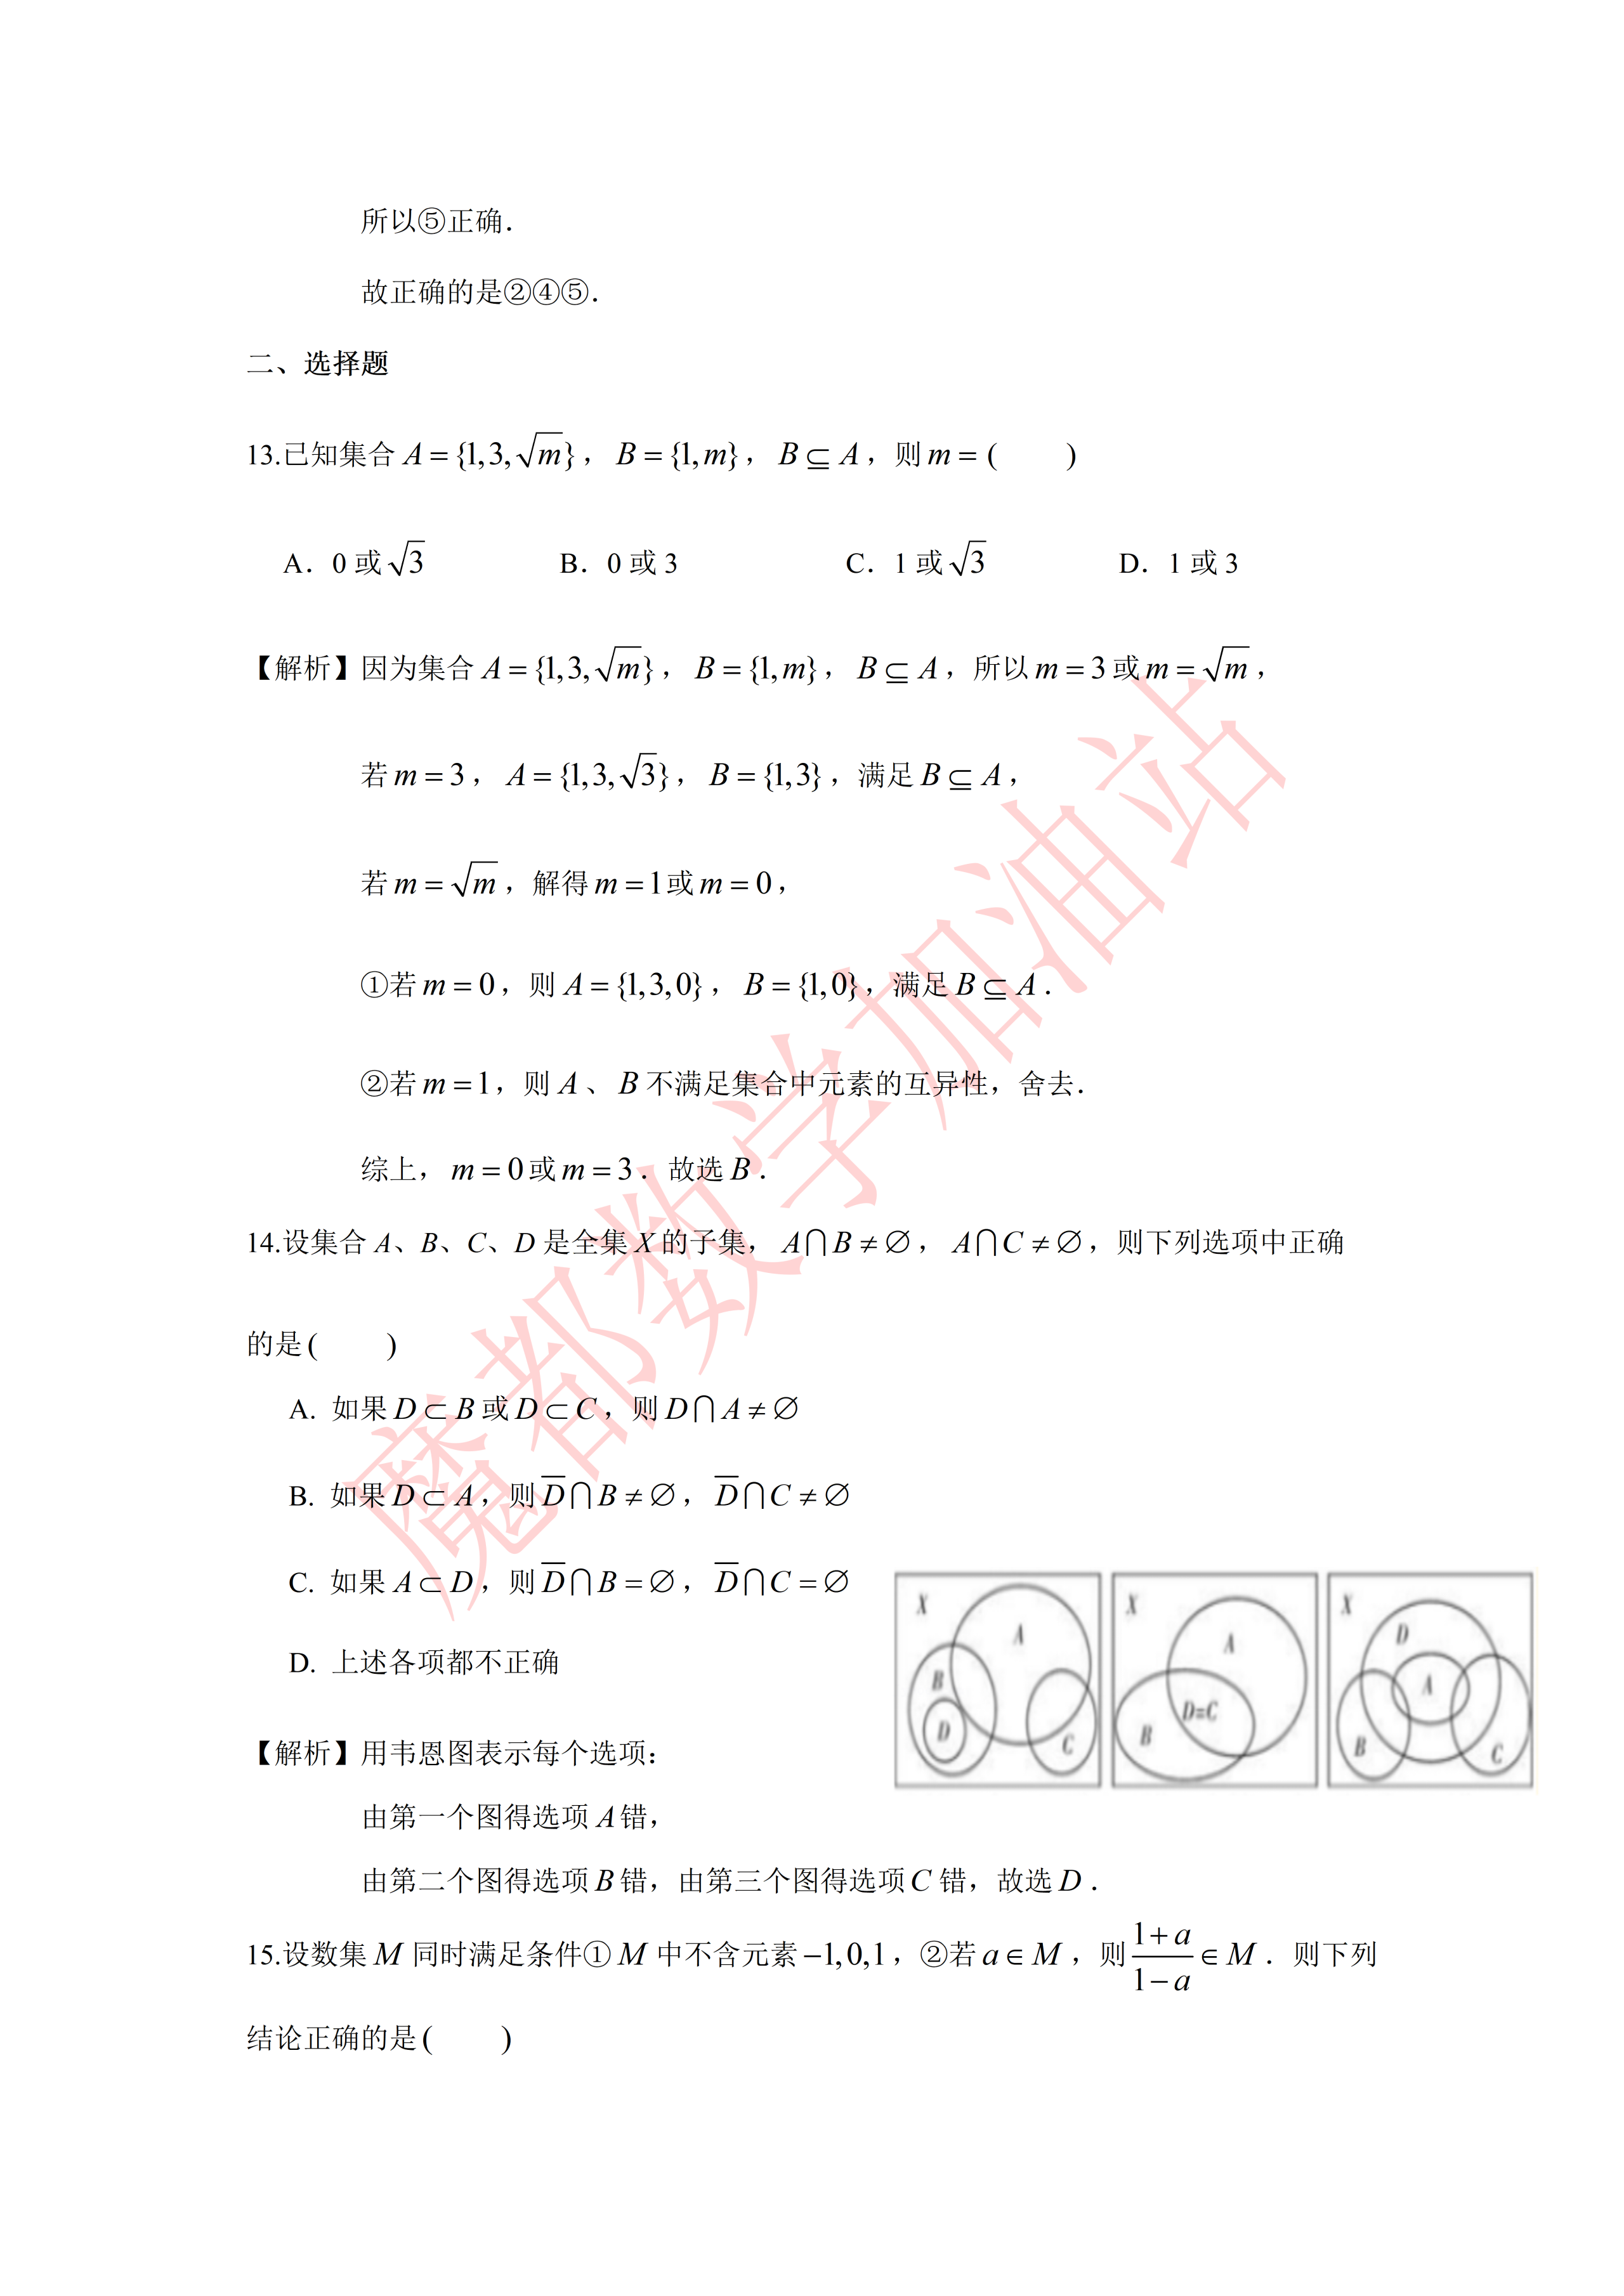
\includegraphics[width=.75\linewidth,trim=1400bp 790bp 135bp 1155bp,clip]{../原图/高一49_华师大二附中_国庆作业1/05.png}
\end{center}
\step{由第一个图得选项 $A$ 错，}
\step{由第二个图得选项 $B$ 错，由第三个图得选项 $C$ 错，故选 $D$.}
\solend
\fi

\item 设数集 $M$ 同时满足条件①$M$ 中不含元素 $-1$、$0$、$1$，②若 $a\in M$，则 $\dfrac{1+a}{1-a}\in M$．则下列结论正确的是\mbox{（\quad）}

\keepwithprev
A. 集合 $M$ 中至多有 $2$ 个元素\qquad B. 集合 $M$ 中至多有 $3$ 个元素

C. 集合 $M$ 中有且仅有 $4$ 个元素\qquad D. 集合 $M$ 中有无穷多个元素

\ifanswer
\solbegin
\step{若集合只含有一个元素，则 $\dfrac{1+a}{1-a}=a$，即 $1+a=a-a^2$，即 $-a^2=1$，不成立.}
\step{当 $a=3$ 时，$\dfrac{1+3}{1-3}=-2\in M$，所以 $\dfrac{1-2}{1+2}=-\dfrac13\in M$，所以 $\dfrac{1-\frac13}{1+\frac13}=\dfrac12\in M$，}
\step{所以 $\dfrac{1+\frac12}{1-\frac12}=3$，开始重复了，所以 $M=\left\{3,-2,-\dfrac13,\dfrac12\right\}$；}
\step{当 $a=2$ 时，$\dfrac{1+2}{1-2}=-3\in M$，所以 $\dfrac{1-3}{1+3}=-\dfrac12\in M$，所以 $\dfrac{1-\frac12}{1+\frac12}=\dfrac13\in M$，}
\step{所以 $\dfrac{1+\frac13}{1-\frac13}=2$，开始重复了，所以 $M=\left\{2,-3,-\dfrac12,-\dfrac13\right\}$，}
\step{此时也只要四个元素；}
\step{当 $a=\dfrac34\in M$，则 $7\in M$，若 $7\in M$，则 $-\dfrac43\in M$，}
\step{若 $-\dfrac43\in M$，则 $-\dfrac17\in M$，若 $-\dfrac17\in M$，有 $\dfrac34\in M$，}
\step{由归纳推理得，集合 $M$ 中有且仅有 $4$ 个元素．故选 $C$.}
\solend
\fi

\item 已知集合 $M=\{x\mid x\in\N,0<x\leqslant15\}$，$A_1$、$A_2$、$A_3$ 满足：①$A_1\cup A_2\cup A_3=M$；②每个集合都恰有 $5$ 个元素．集合 $A_i$（$i=1,2,3$）中最大元素与最小元素之和称为 $A_i$ 的特征数，记为 $X_i$（$i=1,2,3$），则 $X_1+X_2+X_3$ 的值不可能为\mbox{（\quad）}

\keepwithprev
A. $37$\qquad B. $39$\qquad C. $48$\qquad D. $57$

\ifanswer
\solbegin
\step{因为集合 $M=\{x\mid x\in\N,0<x\leqslant15\}=\{1,2,3,\cdots,15\}$，}
\step{又因为集合 $A_1$、$A_2$、$A_3$ 中，每个集合恰有 $5$ 个元素，}
\step{且 $A_1\cup A_2\cup A_3=M$ 有 $15$ 个元素，所以集合 $A_1$、$A_2$、$A_3$ 中没有重复元素，}
\step{因为 $1$ 是集合 $M$ 中数值最小的元素，$15$ 是集合 $M$ 中数值最大的元素，}
\step{所以在 $A_i$ 的特征数构成中，必有 $1$ 和 $15$，不妨设 $1\in A_1$，$15\in A_1$，}
\step{要使 $X_1+X_2+X_3$ 最大，则应该在集合 $A_1$ 中首先放置数值较小的元素，}
\step{即 $A_1=\{1,2,3,4,15\}$，所以 $5$ 与 $14$ 是剩下元素中数值最小或最大的元素，}
\step{同理，不妨设 $5\in A_2$，$14\in A_2$，接着在 $A_2$ 中再次放置数值较小的元素，}
\step{即 $A_2=\{5,6,7,8,14\}$，则 $A_3=\{9,10,11,12,13\}$，}
\step{此时 $X_1+X_2+X_3$ 有最大值为 $1+15+5+14+9+13=57$，}
\step{即 $X_1+X_2+X_3\leqslant57$；}
\step{要使 $X_1+X_2+X_3$ 最小，则在集合 $A_1$ 中首先放置数值较大的元素，}
\step{即 $A_1=\{1,12,13,14,15\}$，所以 $2$ 与 $11$ 是剩下元素中数值最小或最大的元素，}
\step{同理，不妨设 $2\in A_2$，$11\in A_2$，接着在 $A_2$ 中再次放置数值较大的元素，}
\step{即 $A_2=\{2,8,9,10,11\}$，则 $A_3=\{3,4,5,6,7\}$，}
\step{此时 $X_1+X_2+X_3$ 有最小值为 $1+15+2+11+3+7=39$，}
\step{即 $X_1+X_2+X_3\geqslant39$，}
\step{综上，$39\leqslant X_1+X_2+X_3\leqslant57$，故选 $A$.}
\solend
\fi

\end{enumerate}

\bigsec{三、解答题}

\begin{enumerate}
\setcounter{enumi}{16}

\item 已知全集为 $\R$，集合 $A=\{x\mid y=\sqrt{(2+x)(4-x)}\}$，$B=\{x\mid-1<x<m+1\}$.

\begin{enumerate}[label=(\arabic*)]
\item 若 $m=4$，求 $A\cup B$、$\overline A\cap B$；
\item 若 $B\subseteq A$，求实数 $m$ 的取值范围.
\end{enumerate}

\ifanswer
\solbegin
\stepm{(1)}{集合 $A=\{x\mid y=\sqrt{(2+x)(4-x)}\}=\{x\mid-2\leqslant x\leqslant4\}$，}
\step{当 $m=4$ 时，$B=\{x\mid-1<x<5\}$.}
\step{所以 $A\cup B=[-2,5)$，$\overline A=\{x\mid x<-2\text{ 或 }x>4\}$，$\overline A\cap B=(4,5)$.}
\stepm{(2)}{因为 $B\subseteq A$，}
% 原卷如此，照录未改（第 17 题(2)解析两处"当 C=∅／当 C≠∅"应为 B，本卷并无集合 C）
\step{当 $C=\varnothing$ 时，$m\leqslant-2$，$B\subseteq A$ 成立；}
\step{当 $C\neq\varnothing$ 时，$m>-2$，$-1<m+1\leqslant4$，解得 $-2<m\leqslant3$，}
\step{综上，$m\leqslant3$，所以实数 $m$ 的取值范围是 $(-\infty,3]$.}
\solend
\fi

\ansspace[6]

\item 用反证法证明：若 $a$、$b$、$c\in\R$，且 $x=a^2-2b+1$，$y=b^2-2c+1$，$z=c^2-2a+1$，则 $x$、$y$、$z$ 中至少有一个不小于 $0$.

\ifanswer
\solbegin
\step{假设 $x$、$y$、$z$ 均小于 $0$，即 $x=a^2-2b+1<0$①，$y=b^2-2c+1<0$②，}
\step{$z=c^2-2a+1<0$③，①$+$②$+$③得 $x+y+z=(a-1)^2+(b-1)^2+(c-1)^2<0$，}
\step{这与 $(a-1)^2+(b-1)^2+(c-1)^2\geqslant0$ 矛盾，则假设不成立，}
\step{所以 $x$、$y$、$z$ 中至少有一个不小于 $0$，得证.}
\solend
\fi

\ansspace[5]

\item 已知全集为 $\R$，实数 $a$、$b$ 满足 $a\neq b$，集合 $M=\{x\mid x^2-3x-4\leqslant0\}$，集合 $A=\{x\mid(x+a)(x+b)>0\}$，集合 $B=\{x\mid x^2+(a-2)x-2a>0\}$.

\begin{enumerate}[label=(\arabic*)]
\item 若 $\overline A=M$，求 $a$、$b$ 的值；
\item 若 $a>b>-1$，求 $A\cap B$；
\item 若 $a^2+a\in\overline B$，求 $a$ 的取值范围.
\end{enumerate}

\ifanswer
\solbegin
\stepm{(1)}{$M=\{x\mid x^2-3x-4\leqslant0\}=\{x\mid-1\leqslant x\leqslant4\}$，$A=\{x\mid(x+a)(x+b)\leqslant0\}$，}
\step{因为 $\overline A=M$，所以 $a=1$，$b=-4$ 或 $a=-4$，$b=1$.}
\stepm{(2)}{因为 $a>b>-1$，所以 $-a<-b<1$，所以 $A=\{x\mid x<-a\text{ 或 }x>-b\}$，}
\step{因为 $B=\{x\mid x^2+(a-2)x-2a>0\}=\{x\mid x<-a\text{ 或 }x>2\}$，}
\step{所以 $A\cap B=\{x\mid x<-a\text{ 或 }x>2\}$，}
\stepm{(3)}{$\overline B=\{x\mid(x-2)(x+a)\leqslant0\}$，}
% 原卷如此，照录未改（第 19 题(3)此处"a(a-1)((a-2)^2≤0"括号不配对；且由左式展开应为
% a(a-1)(a+2)^2≤0，与下句"解得 a=2 …[0,1]∪{2}"按 (a-2)^2 方自洽，见文件头清单第 2 条）
\step{由 $a^2+a\in\overline B$，得 $(a^2+a-2)(a^2+2a)\leqslant0\Leftrightarrow a(a-1)((a-2)^2\leqslant0$，}
\step{解得 $a=2$ 或 $0\leqslant a\leqslant1$，故 $a$ 的取值范围是 $[0,1]\cup\{2\}$.}
\solend
\fi

\ansspace[7]

\item 设数集 $A$ 由实数构成，若 $x\in A$（$x\neq1$ 且 $x\neq0$），则 $\dfrac{1}{1-x}\in A$.

\begin{enumerate}[label=(\arabic*)]
\item 若 $2\in A$，则 $A$ 中至少还有几个元素；
\item 集合 $A$ 是否为双元素集合？请说明理由；
\item 若 $A$ 中元素个数不超过 $8$ 个，所有元素的和为 $\dfrac{14}{3}$，且 $A$ 中有一个元素的平方等于所有元素的积，求集合 $A$.
\end{enumerate}

\ifanswer
\solbegin
\stepm{(1)}{若 $x\in A$，则 $\dfrac{1}{1-x}\in A$，又 $2\in A$，所以 $\dfrac{1}{1-2}=-1\in A$，}
\step{所以 $\dfrac{1}{1-(-1)}=\dfrac12\in A$，所以 $\dfrac{1}{1-\frac12}=2\in A$，}
% 原卷如此，照录未改（第 20 题(1)解析末句"2 个几个元素"衍一"几个"）
\step{所以 $A$ 中至少还有 $2$ 个几个元素；}
\stepm{(2)}{若 $x\in A$（$x\neq1$ 且 $x\neq0$），则 $\dfrac{1}{1-x}\in A$，}
\step{则 $\dfrac{1}{1-\frac{1}{1-x}}=\dfrac{1-x}{-x}\in A$，则 $\dfrac{1}{1-\frac{1-x}{-x}}=x\in A$}
\step{若 $A$ 为双元素集，则 $x=\dfrac{1}{1-x}$ 或 $x=\dfrac{1-x}{-x}$ 或 $\dfrac{1}{1-x}=\dfrac{1-x}{-x}$，均无解，}
\step{所以 $A$ 不可能为双元素集；}
\stepm{(3)}{由 $x\in A$，$\dfrac{1}{1-x}\in A$，得 $\dfrac{1}{1-\frac{1}{1-x}}=\dfrac{x-1}{x}\in A$，得 $\dfrac{1}{1-\frac{x-1}{x}}=x\in A$，}
\step{所以 $\left\{x,\dfrac{1}{1-x},\dfrac{x-1}{x}\right\}\subseteq A$，而 $x\cdot\dfrac{1}{1-x}\cdot\dfrac{x-1}{x}=-1$，}
\step{$A$ 中元素个数为 $3$ 的倍数，则 $A$ 中元素只有 $6$ 个，}
\step{因为 $A$ 中有一个元素的平方等于所有元素的积，}
\step{不妨设 $x^2=1$，解得 $x=-1$ 或 $x=1$（舍），则 $-1$、$\dfrac12$、$2\in A$，}
\step{所以 $-1+\dfrac12+2+m+\dfrac{1}{1-m}+\dfrac{m-1}{m}=\dfrac{14}{3}$，解得 $m=-\dfrac12$ 或 $m=3$ 或 $m=\dfrac23$，}
\step{所以 $A=\left\{\dfrac12,2,-1,-\dfrac12,3,\dfrac23\right\}$.}
\solend
\fi

\ansspace[9]

% 原卷如此，照录未改（第 21 题题干"21.求已知集合"之"求"字疑衍；"任意两个元素 a_i a_j"
% 疑脱逗号；"|a_i-a_j|≥1/30 则称"之前疑脱标点，见文件头清单第 4 条）
\item 求已知集合 $M=\left\{\dfrac{1}{k}\middle|1\leqslant k\leqslant100\text{ 且 }k\in\N^{*}\right\}$，$A=\{a_1,a_2,\cdots,a_n\}$，其中 $n\in\N^{*}$，且 $n\geqslant2$．若 $A\subseteq\N$，且对集合 $A$ 中的任意两个元素 $a_ia_j$，$i\neq j$ 都有 $|a_i-a_j|\geqslant\dfrac{1}{30}$ 则称集合 $A$ 有性质 $P$.

\begin{enumerate}[label=(\arabic*)]
\item 判断集合 $\left\{\dfrac13,\dfrac14,\dfrac15,\dfrac16,\dfrac17\right\}$ 是否具有性质 $P$；
\item 若集合 $A=\{a_1,a_2,\cdots,a_n\}$ 具有性质 $P$.

①求证：$a_i-a_j$ 的最大值大于等于 $\dfrac{n-1}{30}$；

②求 $A$ 的元素个数 $n$ 的最大值.
\end{enumerate}

\ifanswer
\solbegin
\stepm{(1)}{集合为 $\left\{\dfrac13,\dfrac14,\dfrac15,\dfrac16,\dfrac17\right\}$，又 $\dfrac16-\dfrac17=\dfrac{1}{42}<\dfrac{1}{30}$，所以该集合不具有性质 $P$；}
\stepm{(2)}{①因为集合 $A=\{a_1,a_2,\cdots,a_n\}$ 具有性质 $P$，}
\step{不妨设 $a_1<a_2<a_3<\cdots<a_n$，则 $a_i-a_j\geqslant\dfrac{1}{30}$（$i>j$），}
\step{所以 $a_n-a_1=(a_n-a_{n-1})+(a_{n-1}-a_{n-2})+\cdots+(a_2-a_1)\geqslant\dfrac{n-1}{30}$，}
\step{故 $a_i-a_j$ 的最大值大于等于 $\dfrac{n-1}{30}$；}
% 原卷如此，照录未改（第 21 题(2)②首行"a_2-a_1≥(n-1)/30"：由①同款推理只能得
% a_2-a_1≥1/30，见文件头清单第 5 条）
\step{②$A=\{a_1,a_2,\cdots,a_n\}$，不妨设 $a_1<a_2<a_3<\cdots<a_n$，}
\step{要使 $A$ 的元素个数 $n$ 最大，}
\step{则 $A$ 中的元素满足 $a_n=\dfrac{1}{k}$，$a_{n-1}=\dfrac{1}{k+1}$，$\cdots$，$a_1=\dfrac{1}{k+n-1}$（$k\in\N^{*}$），}
\step{又由①得 $a_2-a_1=\dfrac{1}{k+n-2}-\dfrac{1}{k+n-1}\geqslant\dfrac{n-1}{30}$，}
\step{所以 $(k+n-2)(k+n-1)\leqslant30$，又 $a_n-a_{n-1}=\dfrac{1}{k}-\dfrac{1}{k+1}\geqslant\dfrac{1}{30}$，}
\step{所以 $k(k+1)\leqslant30$，所以 $1\leqslant k\leqslant5$（$k\in\N^{*}$），}
\step{当 $k=5$ 时，由 $(k+n-2)(k+n-1)\leqslant30$，解得 $n\leqslant2$，$n\in\N^{*}$；}
\step{当 $k=4$ 时，由 $(k+n-2)(k+n-1)\leqslant30$，解得 $n\leqslant3$，$n\in\N^{*}$；}
\step{当 $k=3$ 时，由 $(k+n-2)(k+n-1)\leqslant30$，解得 $n\leqslant4$，$n\in\N^{*}$；}
\step{当 $k=2$ 时，由 $(k+n-2)(k+n-1)\leqslant30$，解得 $n\leqslant5$，$n\in\N^{*}$；}
\step{当 $k=1$ 时，由 $(k+n-2)(k+n-1)\leqslant30$，解得 $n\leqslant6$，$n\in\N^{*}$.}
\step{故 $A$ 的元素个数 $n$ 的最大值为 $6$，此时集合 $A=\left\{1,\dfrac12,\dfrac13,\cdots,\dfrac16\right\}$.}
\solend
\fi

\ansspace*[10]

\end{enumerate}

\end{document}
"
% 紧凑版：xelatex "\def\iscompact{1}% 高一49_华师大二附中_国庆作业1.tex
%   —— 高一上数学"2026-2027 年华师大二附中高一上国庆作业 1"（讲评版）
% 试卷版：xelatex 高一49_华师大二附中_国庆作业1.tex
% 答案版：xelatex "\def\isanswer{1}% 高一49_华师大二附中_国庆作业1.tex
%   —— 高一上数学"2026-2027 年华师大二附中高一上国庆作业 1"（讲评版）
% 试卷版：xelatex 高一49_华师大二附中_国庆作业1.tex
% 答案版：xelatex "\def\isanswer{1}\input{高一49_华师大二附中_国庆作业1.tex}"
% 紧凑版：xelatex "\def\iscompact{1}\input{高一49_华师大二附中_国庆作业1.tex}"
%
% 原始材料：微信公众号"魔都数学加油站"文章，作者破晓，连载"27学年高一49"；
% 原文标题"27学年高一49——2026-2027年上海市华师大二附中高一上国庆作业1集合与逻辑、
% 等式与不等式的性质"；页面用 JS 渲染，未见明确发布日期（页内时间戳 ≈ 2026-10-05 21:37）；
% 原文链接：https://mp.weixin.qq.com/s/XxZTOBVQslK5cZm2_BbhOg。
% 正文为 11 张 PNG 页：第 01、03、04、06、07、08、09 页 4762×6735，
% 第 02、05、10、11 页 2560×3620，均按页序读取；粉色斜排"魔都数学加油站"为卷面水印，
% 与公众号页脚一并未录入。全卷 11 页均为试卷页，无二维码/宣传页。
%
% 题号与分节：原文自第 3 题起编，填空题 3—12、选择题 13—16、解答题 17—21，共 19 题。
% 讲评版：原卷每题下直接印【答案】或【解析】——只印【答案】的 3 题（第 3、5、8 题），
% 其余 16 题均只印【解析】；解析行数已逐题按印刷行照录（一条 \step＝原卷一个印刷行）。
%
% 卷首标题：照卷面印作"2026-2027 年华师大二附中高一上国庆作业 1"（公众号标题中的"上海市"
% 卷面没有，本稿照卷面），年份区间按全稿惯例排 en dash；副标题照卷面自印的
% "集合与逻辑单元综合检测"（原卷页首标题行下方即印此行，故不另按模块口径拟名）。
% 副标题依据：全卷 19 题均为集合与常用逻辑用语内容——集合类 15 题（6—17、19—21 中除
% 反证法题外），逻辑/命题类 3 题（第 3 题否定形式、第 4 题充要条件、第 5 题反证法假设），
% 反证法证明 1 题（第 18 题）；全卷无不等式求解题，公众号标题中"等式与不等式的性质"
% 与卷面实际内容不符。
%
% 与原卷的排版差异：
%   ① 原文从第 3 题起，填空题为 3—12、选择题为 13—16、解答题为 17—21，本稿保留原题号；
%   ② 原卷每题下直接印【答案】/【解析】，本稿按全稿惯例置于答案版；只印【解析】的题
%      不另提 \ans{}（照 高一36 口径），只印【答案】的题仅给 \ans{}；
%   ③ 原卷第 8 题韦恩图排在题干右侧、第 14 题三联韦恩图排在选项（C、D）右侧，
%      本稿分别移至题干下方、解析首步之后居中排，均直接裁取原图页（02.png、05.png）；
%   ④ 数集记号原卷排作斜体/加粗 R、N、Z，本稿统一为 \R、\N、\Z、\N^*；
%      填空横线按全稿惯例排为 \blankline[4.4em]。
%
% 原卷笔误/存疑清单（均照录未改，正文中该处有 % 注）：
%   1. 第 17 题(2)解析两处"当 C=∅／当 C≠∅"应为 B（本卷并无集合 C）；
%   2. 第 19 题(3)解析"a(a-1)((a-2)^2≤0"括号不配对（多一枚左括号）；且由
%      (a^2+a-2)(a^2+2a)≤0 展开应为 a(a-1)(a+2)^2≤0，与原卷结论"解得 a=2 …
%      [0,1]∪{2}"恰按 (a-2)^2 自洽——因式分解与原式不符，结论按 (a-2)^2 自洽，均照录；
%   3. 第 20 题(1)解析末句"至少还有 2 个几个元素"衍一"几个"；
%   4. 第 21 题题干"21.求已知集合"之"求"字疑衍；"任意两个元素 a_i a_j"疑脱逗号；
%      "≥1/30 则称"之前疑脱标点；
%   5. 第 21 题(2)②解析"a_2-a_1≥(n-1)/30"：由①同款推理只能得 a_2-a_1≥1/30，
%      原卷如此，照录未改（后续 (k+n-2)(k+n-1)≤30 即按该行推得）。
%
\documentclass[a4paper,11pt]{article}
\usepackage{common}

\begin{document}

\examtitlest[3]{2026--2027 年华师大二附中高一上国庆作业 1}{集合与逻辑单元综合检测}

\bigsec{一、填空题}

\begin{enumerate}
\setcounter{enumi}{2}

\item “若 $x^2-x-2\leqslant0$，则 $-1\leqslant x\leqslant2$”的否定形式为\blankline[4.4em].

\ifanswer
\ans{若 $x^2-x-2>0$，则 $x<-1$ 或 $x>2$}
\fi

\item 已知 $p:|x-3|<5$，$q:1-a<x<2a-3$，且 $p$ 是 $q$ 的充分非必要条件，则实数 $a$ 的取值范围是\blankline[4.4em].

\ifanswer
\solbegin
\step{由 $|x-3|<5$ 得 $-2<x<8$，}
\step{又 $p$ 是 $q$ 的充分不必要条件，所以 $(-2,8)\subset(1-a,2a-3)$，}
\step{即 $\begin{cases}-2\geqslant1-a\\ 8\leqslant2a-3\\ (2a-3)-(1-a)\neq8-(-2)\end{cases}$，解得 $a\geqslant\dfrac{11}{2}$，实数 $a$ 的取值范围是 $\left[\dfrac{11}{2},+\infty\right)$.}
\solend
\fi

\item 用反证法证明命题“设 $a$、$b\in\R$，则方程 $a_1x^2+b_1x+c_1=0$ 与 $a_2x^2+b_2x+c_2=0$ 至少有一个实根”时要做的假设是\blankline[4.4em].

\ifanswer
\ans{假设 $a$、$b\in\R$，方程 $a_1x^2+b_1x+c_1=0$ 与 $a_2x^2+b_2x+c_2=0$ 都没有实根}
\fi

\item 设集合 $A=\{x\mid x^2-mx+6=0,x\in\R\}$，且 $A\cap\{2,3\}=A$，则实数 $m$ 的取值范围是\blankline[4.4em].

\ifanswer
\solbegin
\step{由 $A\cap\{2,3\}=A$，得 $A\subseteq\{2,3\}$，}
\step{当 $A=\varnothing$ 时，$\Delta=m^2-24<0$，解得 $-2\sqrt6<m<2\sqrt6$；}
\step{当 $A=\{2\}$ 时，$\begin{cases}2^2-2m+6=0\\ \Delta=m^2-24=0\end{cases}$，无解；}
\step{当 $A=\{3\}$ 时，$\begin{cases}3^2-3m+6=0\\ \Delta=m^2-24=0\end{cases}$，无解；}
\step{当 $A=\{2,3\}$ 时，$\begin{cases}3^2-3m+6=0\\ 2^2-2m+6=0\end{cases}$，解得 $m=5$，}
\step{所以实数 $m$ 的取值范围是 $(-2\sqrt6,2\sqrt6)\cup\{5\}$.}
\solend
\fi

\item 已知 $a\in\R$，集合 $A=\left\{x\middle|\dfrac12a-1<x<\dfrac12a+1\right\}$，设关于 $x$ 的不等式 $ax<a^2+x-1$ 的解集为 $B$，若 $A\subset B$，则实数 $a$ 的取值范围为\blankline[4.4em].

\ifanswer
\solbegin
\step{因为 $ax<a^2+x-1$，所以 $(a-1)x<(a-1)(a+1)$，}
\step{①当 $a=1$ 时，$B=\varnothing$，$A\subset B$ 不可能成立；}
\step{②当 $a<1$ 时，$B=\{x\mid x>a+1\}$，因为 $A\subset B$，所以 $\dfrac12a-1\geqslant a+1$，}
\step{即 $a\leqslant-4$；}
\step{③当 $a>1$ 时，$B=\{x\mid x<a+1\}$，因为 $A\subset B$，所以 $\dfrac12a+1\leqslant a+1$，}
\step{即 $a>1$；}
\step{综上所述，实数 $a$ 的取值范围为 $(-\infty,-4]\cup(1,+\infty)$.}
\solend
\fi

\needvspace{8\baselineskip}

\item 已知 $U$ 为全集，$M$、$P$、$S$ 是 $U$ 的三个子集，用交、并、补关系将图中的阴影部分表示出来\blankline[4.4em].

\begin{center}
% 原图第 2 页题旁韦恩图直接裁取（原卷排于题干右侧）。
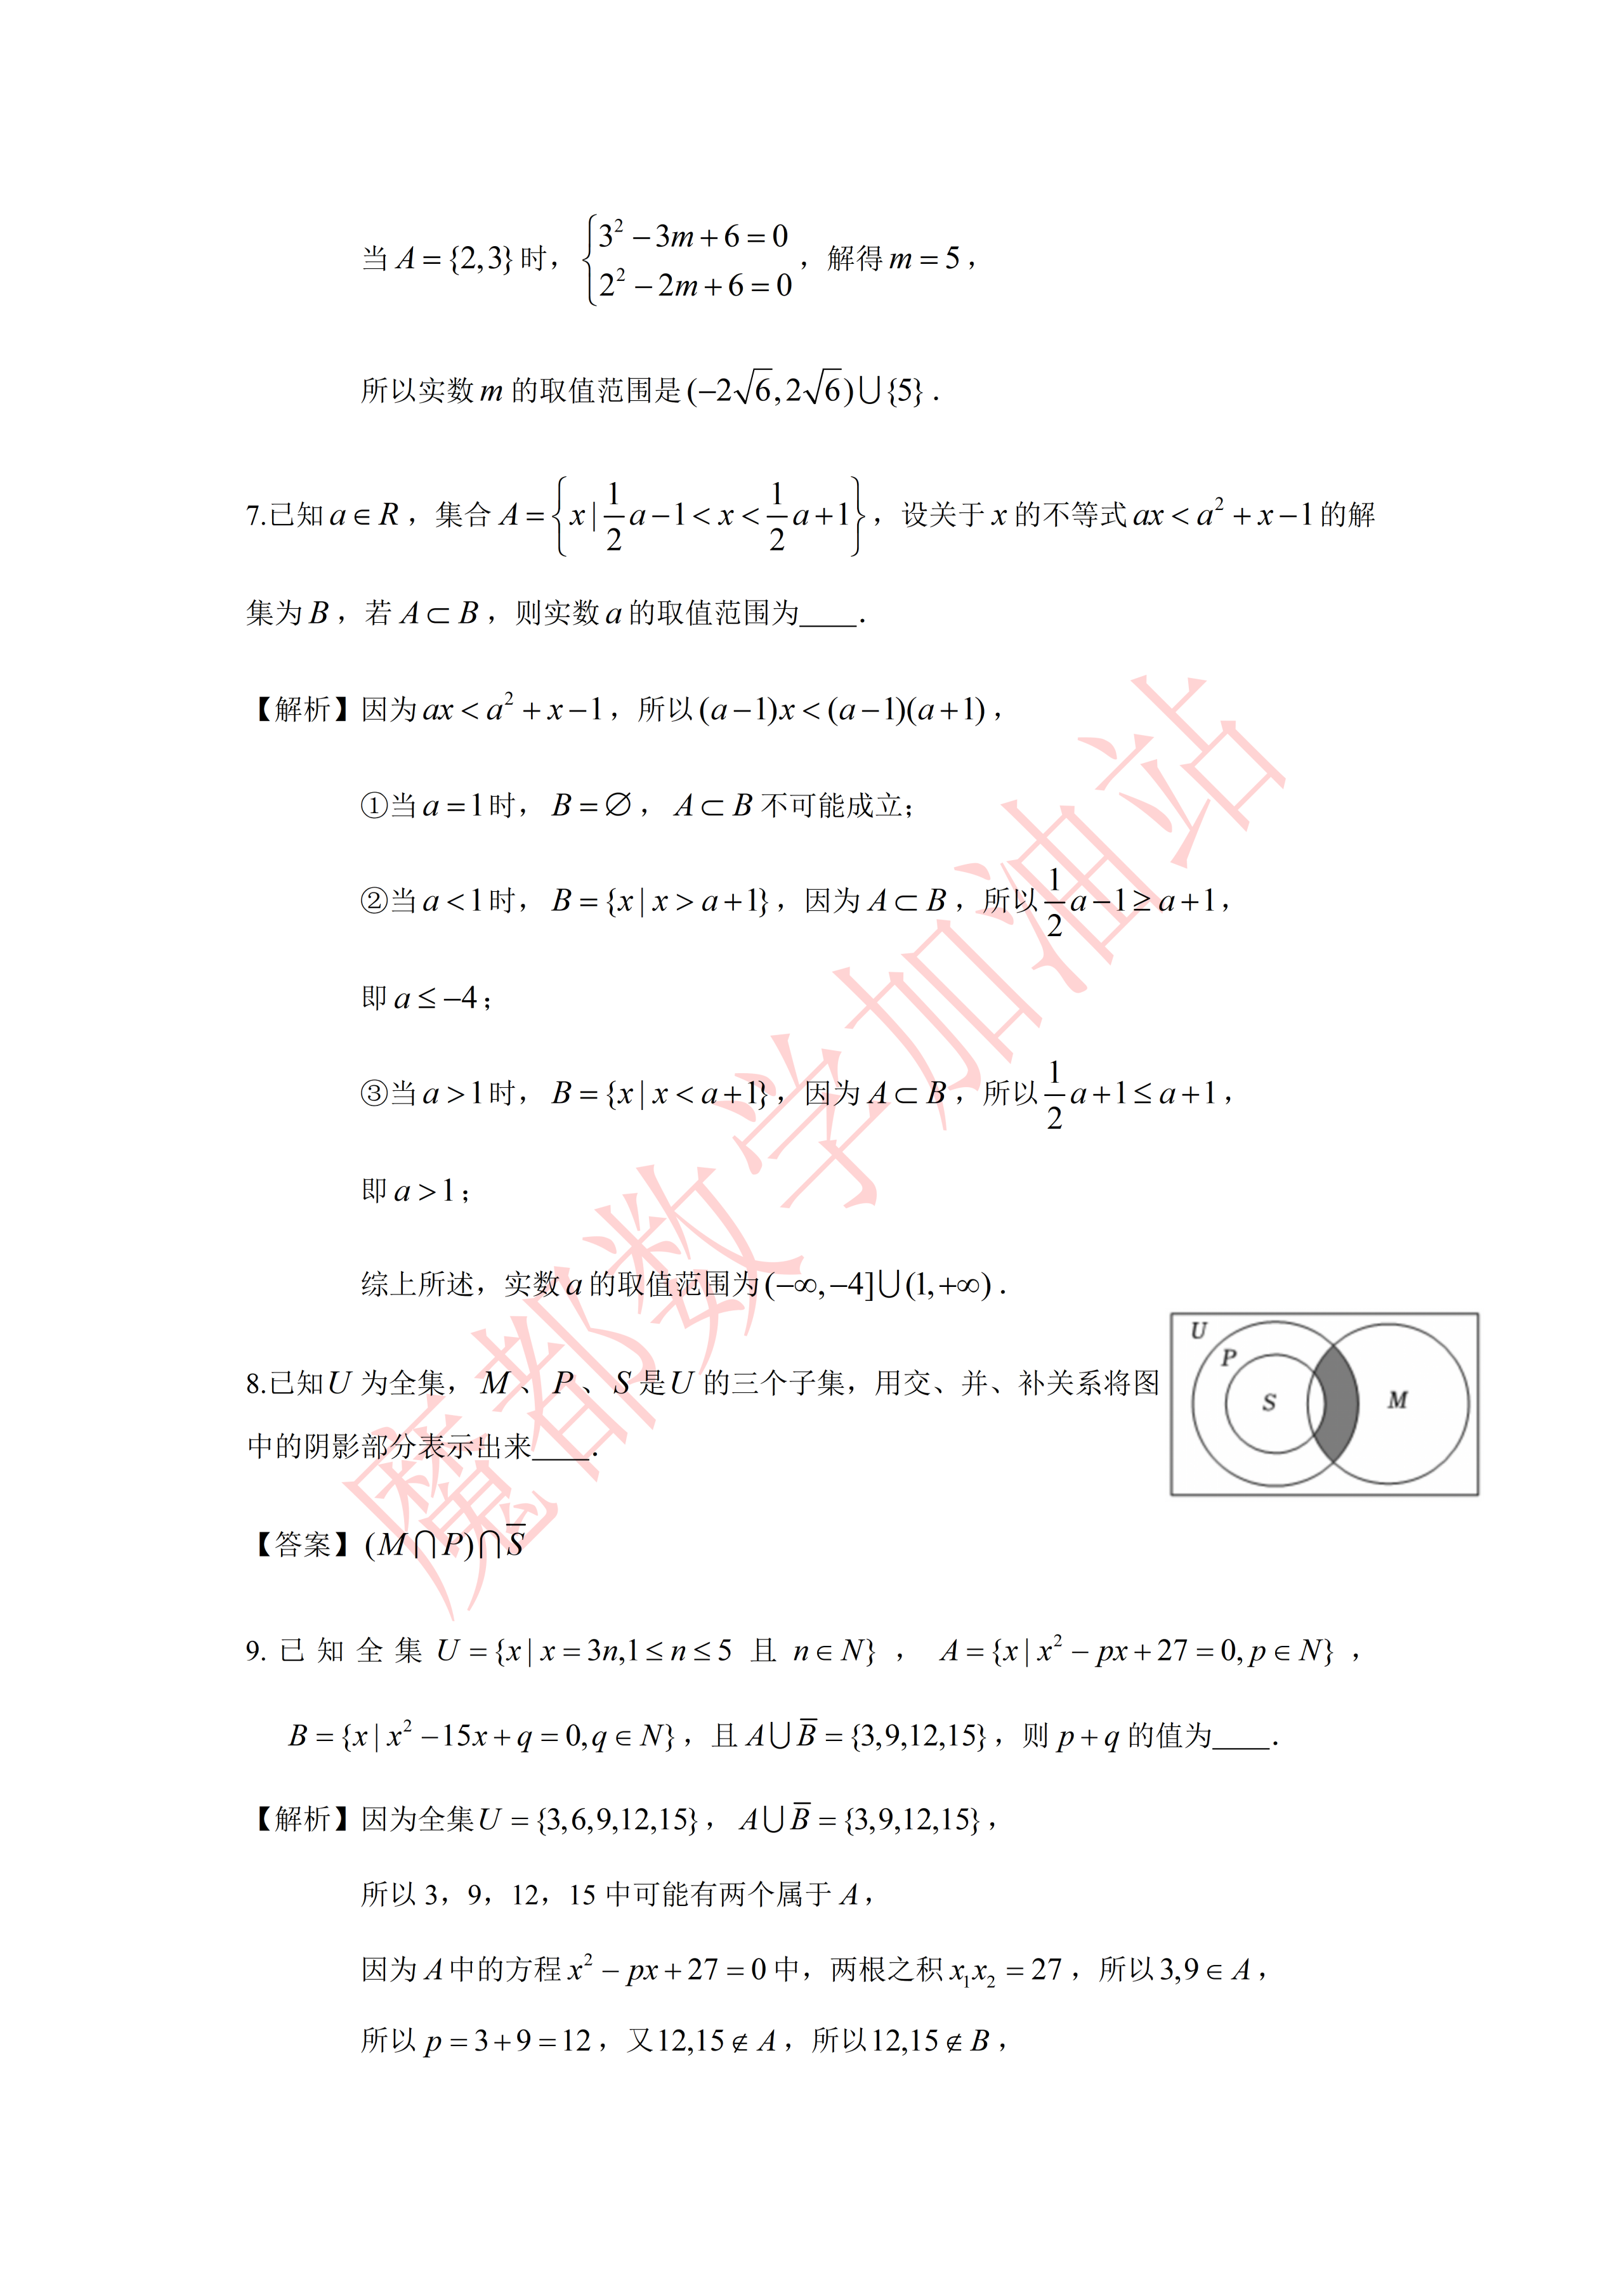
\includegraphics[width=.38\linewidth,trim=1835bp 1255bp 220bp 1565bp,clip]{../原图/高一49_华师大二附中_国庆作业1/02.png}
\end{center}

\ifanswer
\ans{$(M\cap P)\cap\overline S$}
\fi

\item 已知全集 $U=\{x\mid x=3n,1\leqslant n\leqslant5\text{ 且 }n\in\N\}$，$A=\{x\mid x^2-px+27=0,p\in\N\}$，$B=\{x\mid x^2-15x+q=0,q\in\N\}$，且 $A\cup\overline B=\{3,9,12,15\}$，则 $p+q$ 的值为\blankline[4.4em].

\ifanswer
\solbegin
\step{因为全集 $U=\{3,6,9,12,15\}$，$A\cup\overline B=\{3,9,12,15\}$，}
\step{所以 $3$、$9$、$12$、$15$ 中可能有两个属于 $A$，}
\step{因为 $A$ 中的方程 $x^2-px+27=0$ 中，两根之积 $x_1x_2=27$，所以 $3,9\in A$，}
\step{所以 $p=3+9=12$，又 $12,15\notin A$，所以 $12,15\notin B$，}
\step{因为 $B$ 中的方程 $x^2-15x+q=0$ 中，两根之和 $x_3+x_4=15$，所以 $6,9\in B$，}
\step{则 $q=6\times9=54$，所以 $p+q=66$.}
\solend
\fi

\item 已知集合 $A=\{x\mid x^2+(2a-3)x-3a=0,a\in\R,x\in\R\}$，集合 $B=\{x\mid x^2+(a-3)x+a^2-3a=0,a\in\R,x\in\R\}$，若 $A\neq B$，$A\cap B\neq\varnothing$，则 $A\cup B=$\blankline[4.4em].

\ifanswer
\solbegin
\step{设两个集合中的方程的公共解是 $b$，}
\step{由 $b^2+(2a-3)b-3a=b^2+(a-3)b+a^2-3a$，得 $ab=a^2$，}
\step{则 $a=0$ 或 $b=a$，}
\step{当 $a=0$ 时，不合题意，}
\step{当 $b=a$ 时，即两个方程的公共解为 $b=a$，}
\step{将 $b=a$ 代入方程，得 $a^2=2a$，$a=2$，}
\step{所以 $A=\{2,-3\}$，$B=\{-1,2\}$，所以 $A\cup B=\{-1,2,-3\}$.}
\solend
\fi

\item 已知一个有四个数字元素的集合 $S$，$S$ 的所有子集的元素和（空集的元素和认为是 $0$）的总和为 $16192$，则 $S$ 的元素之和等于\blankline[4.4em].

\ifanswer
\solbegin
\step{设 $S=\{a_1,a_2,a_3,a_4\}$，$S$ 的每个元素在所有子集中均出现 $2^3$ 次，}
\step{故 $(a_1+a_2+a_3+a_4)\cdot2^3=16192$，所以 $a_1+a_2+a_3+a_4=2024$，}
\step{故 $S$ 的元素之和等于 $2024$.}
\solend
\fi

\item 设 $P$ 为非空实数集满足：对任意给定的 $x,y\in P$（$x$、$y$ 可以相同），都有 $x+y\in P,x-y\in P,xy\in P$，则称 $P$ 为封闭集．关于封闭集有下列结论：

①集合 $P=\{-2,-1,0,1,2\}$ 为封闭集；

②集合 $P=\{x\mid x=2n,n\in\Z\}$ 为封闭集；

③若集合 $P_1$、$P_2$ 为封闭集，则 $P_1\cup P_2$ 为封闭集；

④若集合 $P$ 为封闭集，则一定有 $0\in P$；

⑤若集合 $P_1$、$P_2$ 为封闭集，则 $P_1\cap P_2$ 为封闭集.

其中正确结论的序号是\blankline[4.4em].

\ifanswer
\solbegin
\step{对于集合 $P=\{-2,-1,0,1,2\}$，取 $x=2$，$y=-2$，则 $x-y=2-(-2)=4\notin P$，}
\step{不满足封闭集的定义，所以①错误.}
\step{对于集合 $P=\{x\mid x=2n,n\in\Z\}$，设 $x=2n_1$，$y=2n_2$，$n_1,n_2\in\Z$.}
\step{$x+y=2n_1+2n_2=2(n_1+n_2)$，因为 $n_1+n_2\in\Z$，所以 $x+y\in P$.}
\step{$x-y=2n_1-2n_2=2(n_1-n_2)$，因为 $n_1-n_2\in\Z$，所以 $x-y\in P$.}
\step{$xy=2n_1\times2n_2=4n_1n_2=2(2n_1n_2)$，因为 $2n_1n_2\in\Z$，所以 $xy\in P$.}
\step{满足封闭集的定义，所以②正确.}
\step{令 $P_1=\{x\mid x=2n,n\in\Z\}$，$P_2=\{x\mid x=3n,n\in\Z\}$，都是封闭集.}
\step{$P_1\cup P_2$ 中，取 $x=2(x\in P_1)$，$y=3(y\in P_2)$，$x+y=5\notin P_1\cup P_2$，}
\step{不满足封闭集的定义，所以③错误.}
\step{因为对任意 $x\in P$，有 $x-x=0\in P$，}
\step{所以若集合 $P$ 为封闭集，则一定有 $0\in P$，所以④正确.}
\step{因为 $P_1$、$P_2$ 为封闭集，设 $x,y\in P_1\cap P_2$，则 $x,y\in P_1$ 且 $x,y\in P_2$.}
\step{因为 $P_1$ 是封闭集，所以 $x+y\in P_1,x-y\in P_1,xy\in P_1$.}
\step{因为 $P_2$ 是封闭集，所以 $x+y\in P_2,x-y\in P_2,xy\in P_2$.}
\step{所以 $x+y\in P_1\cap P_2,x-y\in P_1\cap P_2,xy\in P_1\cap P_2$，满足封闭集的定义，}
\step{所以⑤正确.}
\step{故正确的是②④⑤.}
\solend
\fi

\end{enumerate}

\bigsec{二、选择题}

\begin{enumerate}
\setcounter{enumi}{12}

\item 已知集合 $A=\{1,3,\sqrt m\}$，$B=\{1,m\}$，$B\subseteq A$，则 $m=$\mbox{（\quad）}

\keepwithprev
A. $0$ 或 $\sqrt3$\qquad B. $0$ 或 $3$

C. $1$ 或 $\sqrt3$\qquad D. $1$ 或 $3$

\ifanswer
\solbegin
\step{因为集合 $A=\{1,3,\sqrt m\}$，$B=\{1,m\}$，$B\subseteq A$，所以 $m=3$ 或 $m=\sqrt m$，}
\step{若 $m=3$，$A=\{1,3,\sqrt3\}$，$B=\{1,3\}$，满足 $B\subseteq A$，}
\step{若 $m=\sqrt m$，解得 $m=1$ 或 $m=0$，}
\step{①若 $m=0$，则 $A=\{1,3,0\}$，$B=\{1,0\}$，满足 $B\subseteq A$.}
\step{②若 $m=1$，则 $A$、$B$ 不满足集合中元素的互异性，舍去.}
\step{综上，$m=0$ 或 $m=3$．故选 $B$.}
\solend
\fi

\needvspace{10\baselineskip}

\item 设集合 $A$、$B$、$C$、$D$ 是全集 $X$ 的子集，$A\cap B\neq\varnothing$，$A\cap C\neq\varnothing$，则下列选项中正确的是\mbox{（\quad）}

\keepwithprev
A. 如果 $D\subset B$ 或 $D\subset C$，则 $D\cap A\neq\varnothing$

B. 如果 $D\subset A$，则 $\overline D\cap B\neq\varnothing$，$\overline D\cap C\neq\varnothing$

C. 如果 $A\subset D$，则 $\overline D\cap B=\varnothing$，$\overline D\cap C=\varnothing$

D. 上述各项都不正确

\ifanswer
\solbegin
\step{用韦恩图表示每个选项：}
\begin{center}
% 原图第 5 页解析配图（三联韦恩图）直接裁取（原卷排于选项 C、D 右侧）。
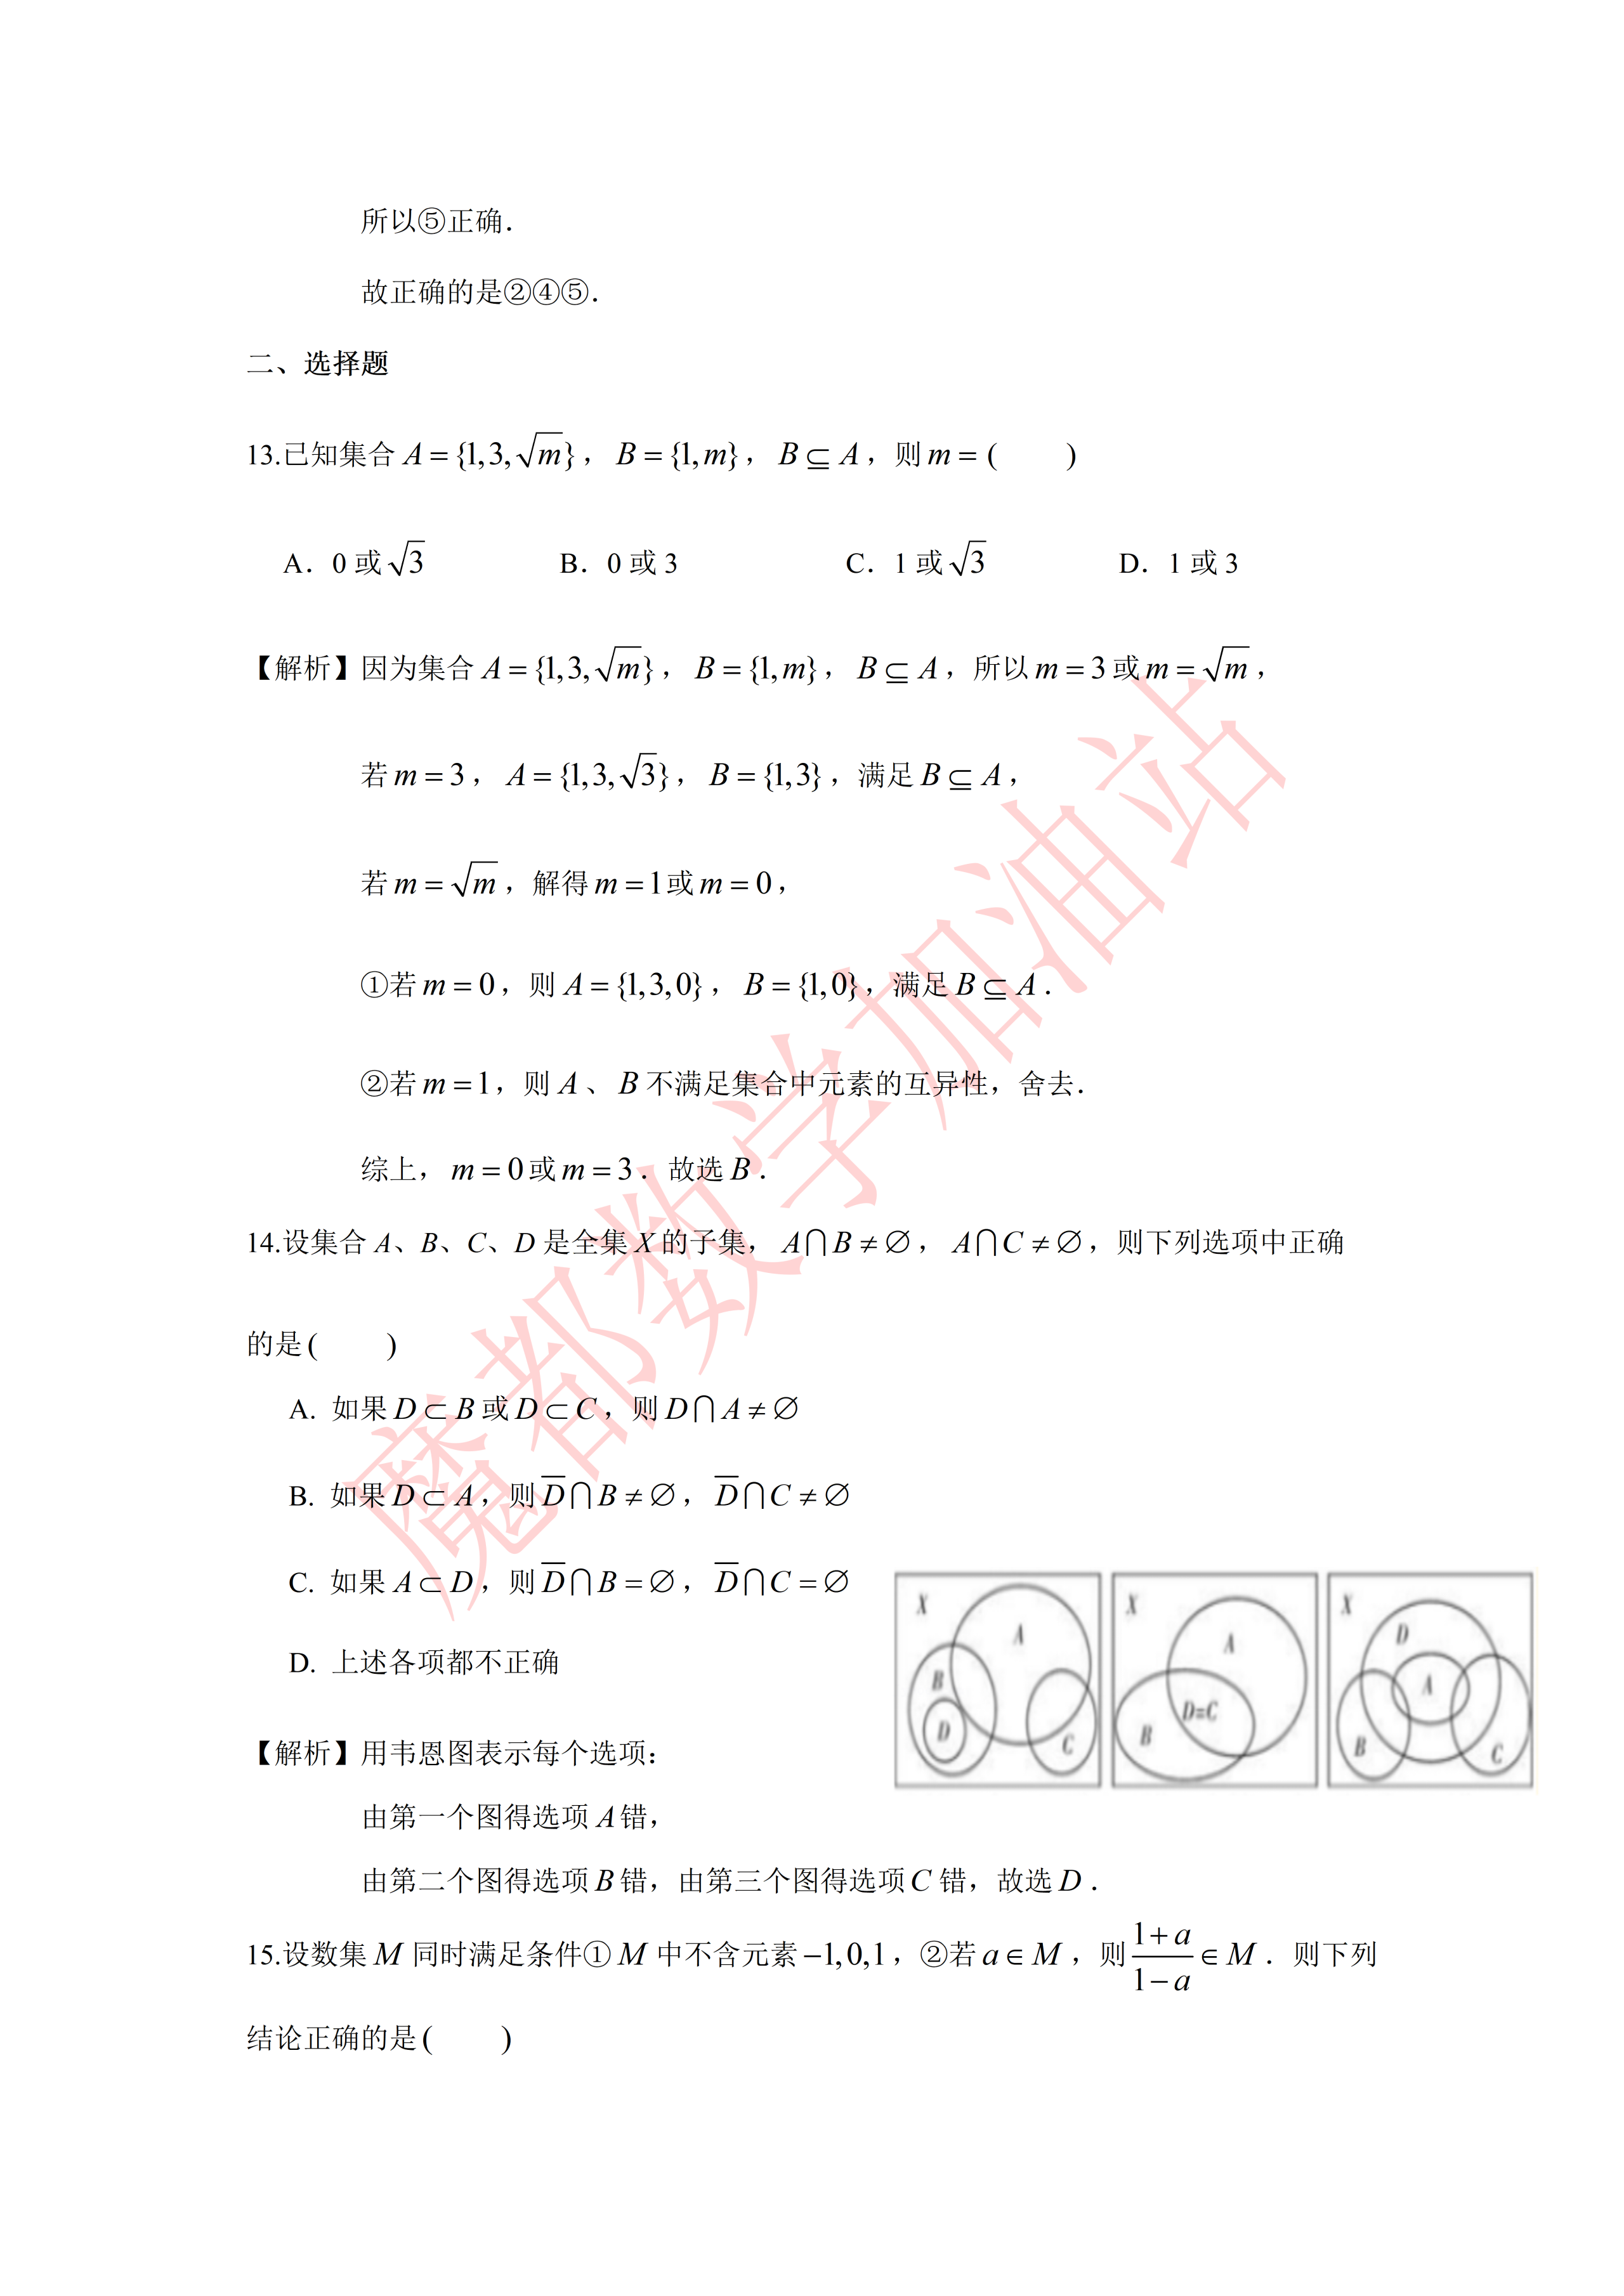
\includegraphics[width=.75\linewidth,trim=1400bp 790bp 135bp 1155bp,clip]{../原图/高一49_华师大二附中_国庆作业1/05.png}
\end{center}
\step{由第一个图得选项 $A$ 错，}
\step{由第二个图得选项 $B$ 错，由第三个图得选项 $C$ 错，故选 $D$.}
\solend
\fi

\item 设数集 $M$ 同时满足条件①$M$ 中不含元素 $-1$、$0$、$1$，②若 $a\in M$，则 $\dfrac{1+a}{1-a}\in M$．则下列结论正确的是\mbox{（\quad）}

\keepwithprev
A. 集合 $M$ 中至多有 $2$ 个元素\qquad B. 集合 $M$ 中至多有 $3$ 个元素

C. 集合 $M$ 中有且仅有 $4$ 个元素\qquad D. 集合 $M$ 中有无穷多个元素

\ifanswer
\solbegin
\step{若集合只含有一个元素，则 $\dfrac{1+a}{1-a}=a$，即 $1+a=a-a^2$，即 $-a^2=1$，不成立.}
\step{当 $a=3$ 时，$\dfrac{1+3}{1-3}=-2\in M$，所以 $\dfrac{1-2}{1+2}=-\dfrac13\in M$，所以 $\dfrac{1-\frac13}{1+\frac13}=\dfrac12\in M$，}
\step{所以 $\dfrac{1+\frac12}{1-\frac12}=3$，开始重复了，所以 $M=\left\{3,-2,-\dfrac13,\dfrac12\right\}$；}
\step{当 $a=2$ 时，$\dfrac{1+2}{1-2}=-3\in M$，所以 $\dfrac{1-3}{1+3}=-\dfrac12\in M$，所以 $\dfrac{1-\frac12}{1+\frac12}=\dfrac13\in M$，}
\step{所以 $\dfrac{1+\frac13}{1-\frac13}=2$，开始重复了，所以 $M=\left\{2,-3,-\dfrac12,-\dfrac13\right\}$，}
\step{此时也只要四个元素；}
\step{当 $a=\dfrac34\in M$，则 $7\in M$，若 $7\in M$，则 $-\dfrac43\in M$，}
\step{若 $-\dfrac43\in M$，则 $-\dfrac17\in M$，若 $-\dfrac17\in M$，有 $\dfrac34\in M$，}
\step{由归纳推理得，集合 $M$ 中有且仅有 $4$ 个元素．故选 $C$.}
\solend
\fi

\item 已知集合 $M=\{x\mid x\in\N,0<x\leqslant15\}$，$A_1$、$A_2$、$A_3$ 满足：①$A_1\cup A_2\cup A_3=M$；②每个集合都恰有 $5$ 个元素．集合 $A_i$（$i=1,2,3$）中最大元素与最小元素之和称为 $A_i$ 的特征数，记为 $X_i$（$i=1,2,3$），则 $X_1+X_2+X_3$ 的值不可能为\mbox{（\quad）}

\keepwithprev
A. $37$\qquad B. $39$\qquad C. $48$\qquad D. $57$

\ifanswer
\solbegin
\step{因为集合 $M=\{x\mid x\in\N,0<x\leqslant15\}=\{1,2,3,\cdots,15\}$，}
\step{又因为集合 $A_1$、$A_2$、$A_3$ 中，每个集合恰有 $5$ 个元素，}
\step{且 $A_1\cup A_2\cup A_3=M$ 有 $15$ 个元素，所以集合 $A_1$、$A_2$、$A_3$ 中没有重复元素，}
\step{因为 $1$ 是集合 $M$ 中数值最小的元素，$15$ 是集合 $M$ 中数值最大的元素，}
\step{所以在 $A_i$ 的特征数构成中，必有 $1$ 和 $15$，不妨设 $1\in A_1$，$15\in A_1$，}
\step{要使 $X_1+X_2+X_3$ 最大，则应该在集合 $A_1$ 中首先放置数值较小的元素，}
\step{即 $A_1=\{1,2,3,4,15\}$，所以 $5$ 与 $14$ 是剩下元素中数值最小或最大的元素，}
\step{同理，不妨设 $5\in A_2$，$14\in A_2$，接着在 $A_2$ 中再次放置数值较小的元素，}
\step{即 $A_2=\{5,6,7,8,14\}$，则 $A_3=\{9,10,11,12,13\}$，}
\step{此时 $X_1+X_2+X_3$ 有最大值为 $1+15+5+14+9+13=57$，}
\step{即 $X_1+X_2+X_3\leqslant57$；}
\step{要使 $X_1+X_2+X_3$ 最小，则在集合 $A_1$ 中首先放置数值较大的元素，}
\step{即 $A_1=\{1,12,13,14,15\}$，所以 $2$ 与 $11$ 是剩下元素中数值最小或最大的元素，}
\step{同理，不妨设 $2\in A_2$，$11\in A_2$，接着在 $A_2$ 中再次放置数值较大的元素，}
\step{即 $A_2=\{2,8,9,10,11\}$，则 $A_3=\{3,4,5,6,7\}$，}
\step{此时 $X_1+X_2+X_3$ 有最小值为 $1+15+2+11+3+7=39$，}
\step{即 $X_1+X_2+X_3\geqslant39$，}
\step{综上，$39\leqslant X_1+X_2+X_3\leqslant57$，故选 $A$.}
\solend
\fi

\end{enumerate}

\bigsec{三、解答题}

\begin{enumerate}
\setcounter{enumi}{16}

\item 已知全集为 $\R$，集合 $A=\{x\mid y=\sqrt{(2+x)(4-x)}\}$，$B=\{x\mid-1<x<m+1\}$.

\begin{enumerate}[label=(\arabic*)]
\item 若 $m=4$，求 $A\cup B$、$\overline A\cap B$；
\item 若 $B\subseteq A$，求实数 $m$ 的取值范围.
\end{enumerate}

\ifanswer
\solbegin
\stepm{(1)}{集合 $A=\{x\mid y=\sqrt{(2+x)(4-x)}\}=\{x\mid-2\leqslant x\leqslant4\}$，}
\step{当 $m=4$ 时，$B=\{x\mid-1<x<5\}$.}
\step{所以 $A\cup B=[-2,5)$，$\overline A=\{x\mid x<-2\text{ 或 }x>4\}$，$\overline A\cap B=(4,5)$.}
\stepm{(2)}{因为 $B\subseteq A$，}
% 原卷如此，照录未改（第 17 题(2)解析两处"当 C=∅／当 C≠∅"应为 B，本卷并无集合 C）
\step{当 $C=\varnothing$ 时，$m\leqslant-2$，$B\subseteq A$ 成立；}
\step{当 $C\neq\varnothing$ 时，$m>-2$，$-1<m+1\leqslant4$，解得 $-2<m\leqslant3$，}
\step{综上，$m\leqslant3$，所以实数 $m$ 的取值范围是 $(-\infty,3]$.}
\solend
\fi

\ansspace[6]

\item 用反证法证明：若 $a$、$b$、$c\in\R$，且 $x=a^2-2b+1$，$y=b^2-2c+1$，$z=c^2-2a+1$，则 $x$、$y$、$z$ 中至少有一个不小于 $0$.

\ifanswer
\solbegin
\step{假设 $x$、$y$、$z$ 均小于 $0$，即 $x=a^2-2b+1<0$①，$y=b^2-2c+1<0$②，}
\step{$z=c^2-2a+1<0$③，①$+$②$+$③得 $x+y+z=(a-1)^2+(b-1)^2+(c-1)^2<0$，}
\step{这与 $(a-1)^2+(b-1)^2+(c-1)^2\geqslant0$ 矛盾，则假设不成立，}
\step{所以 $x$、$y$、$z$ 中至少有一个不小于 $0$，得证.}
\solend
\fi

\ansspace[5]

\item 已知全集为 $\R$，实数 $a$、$b$ 满足 $a\neq b$，集合 $M=\{x\mid x^2-3x-4\leqslant0\}$，集合 $A=\{x\mid(x+a)(x+b)>0\}$，集合 $B=\{x\mid x^2+(a-2)x-2a>0\}$.

\begin{enumerate}[label=(\arabic*)]
\item 若 $\overline A=M$，求 $a$、$b$ 的值；
\item 若 $a>b>-1$，求 $A\cap B$；
\item 若 $a^2+a\in\overline B$，求 $a$ 的取值范围.
\end{enumerate}

\ifanswer
\solbegin
\stepm{(1)}{$M=\{x\mid x^2-3x-4\leqslant0\}=\{x\mid-1\leqslant x\leqslant4\}$，$A=\{x\mid(x+a)(x+b)\leqslant0\}$，}
\step{因为 $\overline A=M$，所以 $a=1$，$b=-4$ 或 $a=-4$，$b=1$.}
\stepm{(2)}{因为 $a>b>-1$，所以 $-a<-b<1$，所以 $A=\{x\mid x<-a\text{ 或 }x>-b\}$，}
\step{因为 $B=\{x\mid x^2+(a-2)x-2a>0\}=\{x\mid x<-a\text{ 或 }x>2\}$，}
\step{所以 $A\cap B=\{x\mid x<-a\text{ 或 }x>2\}$，}
\stepm{(3)}{$\overline B=\{x\mid(x-2)(x+a)\leqslant0\}$，}
% 原卷如此，照录未改（第 19 题(3)此处"a(a-1)((a-2)^2≤0"括号不配对；且由左式展开应为
% a(a-1)(a+2)^2≤0，与下句"解得 a=2 …[0,1]∪{2}"按 (a-2)^2 方自洽，见文件头清单第 2 条）
\step{由 $a^2+a\in\overline B$，得 $(a^2+a-2)(a^2+2a)\leqslant0\Leftrightarrow a(a-1)((a-2)^2\leqslant0$，}
\step{解得 $a=2$ 或 $0\leqslant a\leqslant1$，故 $a$ 的取值范围是 $[0,1]\cup\{2\}$.}
\solend
\fi

\ansspace[7]

\item 设数集 $A$ 由实数构成，若 $x\in A$（$x\neq1$ 且 $x\neq0$），则 $\dfrac{1}{1-x}\in A$.

\begin{enumerate}[label=(\arabic*)]
\item 若 $2\in A$，则 $A$ 中至少还有几个元素；
\item 集合 $A$ 是否为双元素集合？请说明理由；
\item 若 $A$ 中元素个数不超过 $8$ 个，所有元素的和为 $\dfrac{14}{3}$，且 $A$ 中有一个元素的平方等于所有元素的积，求集合 $A$.
\end{enumerate}

\ifanswer
\solbegin
\stepm{(1)}{若 $x\in A$，则 $\dfrac{1}{1-x}\in A$，又 $2\in A$，所以 $\dfrac{1}{1-2}=-1\in A$，}
\step{所以 $\dfrac{1}{1-(-1)}=\dfrac12\in A$，所以 $\dfrac{1}{1-\frac12}=2\in A$，}
% 原卷如此，照录未改（第 20 题(1)解析末句"2 个几个元素"衍一"几个"）
\step{所以 $A$ 中至少还有 $2$ 个几个元素；}
\stepm{(2)}{若 $x\in A$（$x\neq1$ 且 $x\neq0$），则 $\dfrac{1}{1-x}\in A$，}
\step{则 $\dfrac{1}{1-\frac{1}{1-x}}=\dfrac{1-x}{-x}\in A$，则 $\dfrac{1}{1-\frac{1-x}{-x}}=x\in A$}
\step{若 $A$ 为双元素集，则 $x=\dfrac{1}{1-x}$ 或 $x=\dfrac{1-x}{-x}$ 或 $\dfrac{1}{1-x}=\dfrac{1-x}{-x}$，均无解，}
\step{所以 $A$ 不可能为双元素集；}
\stepm{(3)}{由 $x\in A$，$\dfrac{1}{1-x}\in A$，得 $\dfrac{1}{1-\frac{1}{1-x}}=\dfrac{x-1}{x}\in A$，得 $\dfrac{1}{1-\frac{x-1}{x}}=x\in A$，}
\step{所以 $\left\{x,\dfrac{1}{1-x},\dfrac{x-1}{x}\right\}\subseteq A$，而 $x\cdot\dfrac{1}{1-x}\cdot\dfrac{x-1}{x}=-1$，}
\step{$A$ 中元素个数为 $3$ 的倍数，则 $A$ 中元素只有 $6$ 个，}
\step{因为 $A$ 中有一个元素的平方等于所有元素的积，}
\step{不妨设 $x^2=1$，解得 $x=-1$ 或 $x=1$（舍），则 $-1$、$\dfrac12$、$2\in A$，}
\step{所以 $-1+\dfrac12+2+m+\dfrac{1}{1-m}+\dfrac{m-1}{m}=\dfrac{14}{3}$，解得 $m=-\dfrac12$ 或 $m=3$ 或 $m=\dfrac23$，}
\step{所以 $A=\left\{\dfrac12,2,-1,-\dfrac12,3,\dfrac23\right\}$.}
\solend
\fi

\ansspace[9]

% 原卷如此，照录未改（第 21 题题干"21.求已知集合"之"求"字疑衍；"任意两个元素 a_i a_j"
% 疑脱逗号；"|a_i-a_j|≥1/30 则称"之前疑脱标点，见文件头清单第 4 条）
\item 求已知集合 $M=\left\{\dfrac{1}{k}\middle|1\leqslant k\leqslant100\text{ 且 }k\in\N^{*}\right\}$，$A=\{a_1,a_2,\cdots,a_n\}$，其中 $n\in\N^{*}$，且 $n\geqslant2$．若 $A\subseteq\N$，且对集合 $A$ 中的任意两个元素 $a_ia_j$，$i\neq j$ 都有 $|a_i-a_j|\geqslant\dfrac{1}{30}$ 则称集合 $A$ 有性质 $P$.

\begin{enumerate}[label=(\arabic*)]
\item 判断集合 $\left\{\dfrac13,\dfrac14,\dfrac15,\dfrac16,\dfrac17\right\}$ 是否具有性质 $P$；
\item 若集合 $A=\{a_1,a_2,\cdots,a_n\}$ 具有性质 $P$.

①求证：$a_i-a_j$ 的最大值大于等于 $\dfrac{n-1}{30}$；

②求 $A$ 的元素个数 $n$ 的最大值.
\end{enumerate}

\ifanswer
\solbegin
\stepm{(1)}{集合为 $\left\{\dfrac13,\dfrac14,\dfrac15,\dfrac16,\dfrac17\right\}$，又 $\dfrac16-\dfrac17=\dfrac{1}{42}<\dfrac{1}{30}$，所以该集合不具有性质 $P$；}
\stepm{(2)}{①因为集合 $A=\{a_1,a_2,\cdots,a_n\}$ 具有性质 $P$，}
\step{不妨设 $a_1<a_2<a_3<\cdots<a_n$，则 $a_i-a_j\geqslant\dfrac{1}{30}$（$i>j$），}
\step{所以 $a_n-a_1=(a_n-a_{n-1})+(a_{n-1}-a_{n-2})+\cdots+(a_2-a_1)\geqslant\dfrac{n-1}{30}$，}
\step{故 $a_i-a_j$ 的最大值大于等于 $\dfrac{n-1}{30}$；}
% 原卷如此，照录未改（第 21 题(2)②首行"a_2-a_1≥(n-1)/30"：由①同款推理只能得
% a_2-a_1≥1/30，见文件头清单第 5 条）
\step{②$A=\{a_1,a_2,\cdots,a_n\}$，不妨设 $a_1<a_2<a_3<\cdots<a_n$，}
\step{要使 $A$ 的元素个数 $n$ 最大，}
\step{则 $A$ 中的元素满足 $a_n=\dfrac{1}{k}$，$a_{n-1}=\dfrac{1}{k+1}$，$\cdots$，$a_1=\dfrac{1}{k+n-1}$（$k\in\N^{*}$），}
\step{又由①得 $a_2-a_1=\dfrac{1}{k+n-2}-\dfrac{1}{k+n-1}\geqslant\dfrac{n-1}{30}$，}
\step{所以 $(k+n-2)(k+n-1)\leqslant30$，又 $a_n-a_{n-1}=\dfrac{1}{k}-\dfrac{1}{k+1}\geqslant\dfrac{1}{30}$，}
\step{所以 $k(k+1)\leqslant30$，所以 $1\leqslant k\leqslant5$（$k\in\N^{*}$），}
\step{当 $k=5$ 时，由 $(k+n-2)(k+n-1)\leqslant30$，解得 $n\leqslant2$，$n\in\N^{*}$；}
\step{当 $k=4$ 时，由 $(k+n-2)(k+n-1)\leqslant30$，解得 $n\leqslant3$，$n\in\N^{*}$；}
\step{当 $k=3$ 时，由 $(k+n-2)(k+n-1)\leqslant30$，解得 $n\leqslant4$，$n\in\N^{*}$；}
\step{当 $k=2$ 时，由 $(k+n-2)(k+n-1)\leqslant30$，解得 $n\leqslant5$，$n\in\N^{*}$；}
\step{当 $k=1$ 时，由 $(k+n-2)(k+n-1)\leqslant30$，解得 $n\leqslant6$，$n\in\N^{*}$.}
\step{故 $A$ 的元素个数 $n$ 的最大值为 $6$，此时集合 $A=\left\{1,\dfrac12,\dfrac13,\cdots,\dfrac16\right\}$.}
\solend
\fi

\ansspace*[10]

\end{enumerate}

\end{document}
"
% 紧凑版：xelatex "\def\iscompact{1}% 高一49_华师大二附中_国庆作业1.tex
%   —— 高一上数学"2026-2027 年华师大二附中高一上国庆作业 1"（讲评版）
% 试卷版：xelatex 高一49_华师大二附中_国庆作业1.tex
% 答案版：xelatex "\def\isanswer{1}\input{高一49_华师大二附中_国庆作业1.tex}"
% 紧凑版：xelatex "\def\iscompact{1}\input{高一49_华师大二附中_国庆作业1.tex}"
%
% 原始材料：微信公众号"魔都数学加油站"文章，作者破晓，连载"27学年高一49"；
% 原文标题"27学年高一49——2026-2027年上海市华师大二附中高一上国庆作业1集合与逻辑、
% 等式与不等式的性质"；页面用 JS 渲染，未见明确发布日期（页内时间戳 ≈ 2026-10-05 21:37）；
% 原文链接：https://mp.weixin.qq.com/s/XxZTOBVQslK5cZm2_BbhOg。
% 正文为 11 张 PNG 页：第 01、03、04、06、07、08、09 页 4762×6735，
% 第 02、05、10、11 页 2560×3620，均按页序读取；粉色斜排"魔都数学加油站"为卷面水印，
% 与公众号页脚一并未录入。全卷 11 页均为试卷页，无二维码/宣传页。
%
% 题号与分节：原文自第 3 题起编，填空题 3—12、选择题 13—16、解答题 17—21，共 19 题。
% 讲评版：原卷每题下直接印【答案】或【解析】——只印【答案】的 3 题（第 3、5、8 题），
% 其余 16 题均只印【解析】；解析行数已逐题按印刷行照录（一条 \step＝原卷一个印刷行）。
%
% 卷首标题：照卷面印作"2026-2027 年华师大二附中高一上国庆作业 1"（公众号标题中的"上海市"
% 卷面没有，本稿照卷面），年份区间按全稿惯例排 en dash；副标题照卷面自印的
% "集合与逻辑单元综合检测"（原卷页首标题行下方即印此行，故不另按模块口径拟名）。
% 副标题依据：全卷 19 题均为集合与常用逻辑用语内容——集合类 15 题（6—17、19—21 中除
% 反证法题外），逻辑/命题类 3 题（第 3 题否定形式、第 4 题充要条件、第 5 题反证法假设），
% 反证法证明 1 题（第 18 题）；全卷无不等式求解题，公众号标题中"等式与不等式的性质"
% 与卷面实际内容不符。
%
% 与原卷的排版差异：
%   ① 原文从第 3 题起，填空题为 3—12、选择题为 13—16、解答题为 17—21，本稿保留原题号；
%   ② 原卷每题下直接印【答案】/【解析】，本稿按全稿惯例置于答案版；只印【解析】的题
%      不另提 \ans{}（照 高一36 口径），只印【答案】的题仅给 \ans{}；
%   ③ 原卷第 8 题韦恩图排在题干右侧、第 14 题三联韦恩图排在选项（C、D）右侧，
%      本稿分别移至题干下方、解析首步之后居中排，均直接裁取原图页（02.png、05.png）；
%   ④ 数集记号原卷排作斜体/加粗 R、N、Z，本稿统一为 \R、\N、\Z、\N^*；
%      填空横线按全稿惯例排为 \blankline[4.4em]。
%
% 原卷笔误/存疑清单（均照录未改，正文中该处有 % 注）：
%   1. 第 17 题(2)解析两处"当 C=∅／当 C≠∅"应为 B（本卷并无集合 C）；
%   2. 第 19 题(3)解析"a(a-1)((a-2)^2≤0"括号不配对（多一枚左括号）；且由
%      (a^2+a-2)(a^2+2a)≤0 展开应为 a(a-1)(a+2)^2≤0，与原卷结论"解得 a=2 …
%      [0,1]∪{2}"恰按 (a-2)^2 自洽——因式分解与原式不符，结论按 (a-2)^2 自洽，均照录；
%   3. 第 20 题(1)解析末句"至少还有 2 个几个元素"衍一"几个"；
%   4. 第 21 题题干"21.求已知集合"之"求"字疑衍；"任意两个元素 a_i a_j"疑脱逗号；
%      "≥1/30 则称"之前疑脱标点；
%   5. 第 21 题(2)②解析"a_2-a_1≥(n-1)/30"：由①同款推理只能得 a_2-a_1≥1/30，
%      原卷如此，照录未改（后续 (k+n-2)(k+n-1)≤30 即按该行推得）。
%
\documentclass[a4paper,11pt]{article}
\usepackage{common}

\begin{document}

\examtitlest[3]{2026--2027 年华师大二附中高一上国庆作业 1}{集合与逻辑单元综合检测}

\bigsec{一、填空题}

\begin{enumerate}
\setcounter{enumi}{2}

\item “若 $x^2-x-2\leqslant0$，则 $-1\leqslant x\leqslant2$”的否定形式为\blankline[4.4em].

\ifanswer
\ans{若 $x^2-x-2>0$，则 $x<-1$ 或 $x>2$}
\fi

\item 已知 $p:|x-3|<5$，$q:1-a<x<2a-3$，且 $p$ 是 $q$ 的充分非必要条件，则实数 $a$ 的取值范围是\blankline[4.4em].

\ifanswer
\solbegin
\step{由 $|x-3|<5$ 得 $-2<x<8$，}
\step{又 $p$ 是 $q$ 的充分不必要条件，所以 $(-2,8)\subset(1-a,2a-3)$，}
\step{即 $\begin{cases}-2\geqslant1-a\\ 8\leqslant2a-3\\ (2a-3)-(1-a)\neq8-(-2)\end{cases}$，解得 $a\geqslant\dfrac{11}{2}$，实数 $a$ 的取值范围是 $\left[\dfrac{11}{2},+\infty\right)$.}
\solend
\fi

\item 用反证法证明命题“设 $a$、$b\in\R$，则方程 $a_1x^2+b_1x+c_1=0$ 与 $a_2x^2+b_2x+c_2=0$ 至少有一个实根”时要做的假设是\blankline[4.4em].

\ifanswer
\ans{假设 $a$、$b\in\R$，方程 $a_1x^2+b_1x+c_1=0$ 与 $a_2x^2+b_2x+c_2=0$ 都没有实根}
\fi

\item 设集合 $A=\{x\mid x^2-mx+6=0,x\in\R\}$，且 $A\cap\{2,3\}=A$，则实数 $m$ 的取值范围是\blankline[4.4em].

\ifanswer
\solbegin
\step{由 $A\cap\{2,3\}=A$，得 $A\subseteq\{2,3\}$，}
\step{当 $A=\varnothing$ 时，$\Delta=m^2-24<0$，解得 $-2\sqrt6<m<2\sqrt6$；}
\step{当 $A=\{2\}$ 时，$\begin{cases}2^2-2m+6=0\\ \Delta=m^2-24=0\end{cases}$，无解；}
\step{当 $A=\{3\}$ 时，$\begin{cases}3^2-3m+6=0\\ \Delta=m^2-24=0\end{cases}$，无解；}
\step{当 $A=\{2,3\}$ 时，$\begin{cases}3^2-3m+6=0\\ 2^2-2m+6=0\end{cases}$，解得 $m=5$，}
\step{所以实数 $m$ 的取值范围是 $(-2\sqrt6,2\sqrt6)\cup\{5\}$.}
\solend
\fi

\item 已知 $a\in\R$，集合 $A=\left\{x\middle|\dfrac12a-1<x<\dfrac12a+1\right\}$，设关于 $x$ 的不等式 $ax<a^2+x-1$ 的解集为 $B$，若 $A\subset B$，则实数 $a$ 的取值范围为\blankline[4.4em].

\ifanswer
\solbegin
\step{因为 $ax<a^2+x-1$，所以 $(a-1)x<(a-1)(a+1)$，}
\step{①当 $a=1$ 时，$B=\varnothing$，$A\subset B$ 不可能成立；}
\step{②当 $a<1$ 时，$B=\{x\mid x>a+1\}$，因为 $A\subset B$，所以 $\dfrac12a-1\geqslant a+1$，}
\step{即 $a\leqslant-4$；}
\step{③当 $a>1$ 时，$B=\{x\mid x<a+1\}$，因为 $A\subset B$，所以 $\dfrac12a+1\leqslant a+1$，}
\step{即 $a>1$；}
\step{综上所述，实数 $a$ 的取值范围为 $(-\infty,-4]\cup(1,+\infty)$.}
\solend
\fi

\needvspace{8\baselineskip}

\item 已知 $U$ 为全集，$M$、$P$、$S$ 是 $U$ 的三个子集，用交、并、补关系将图中的阴影部分表示出来\blankline[4.4em].

\begin{center}
% 原图第 2 页题旁韦恩图直接裁取（原卷排于题干右侧）。
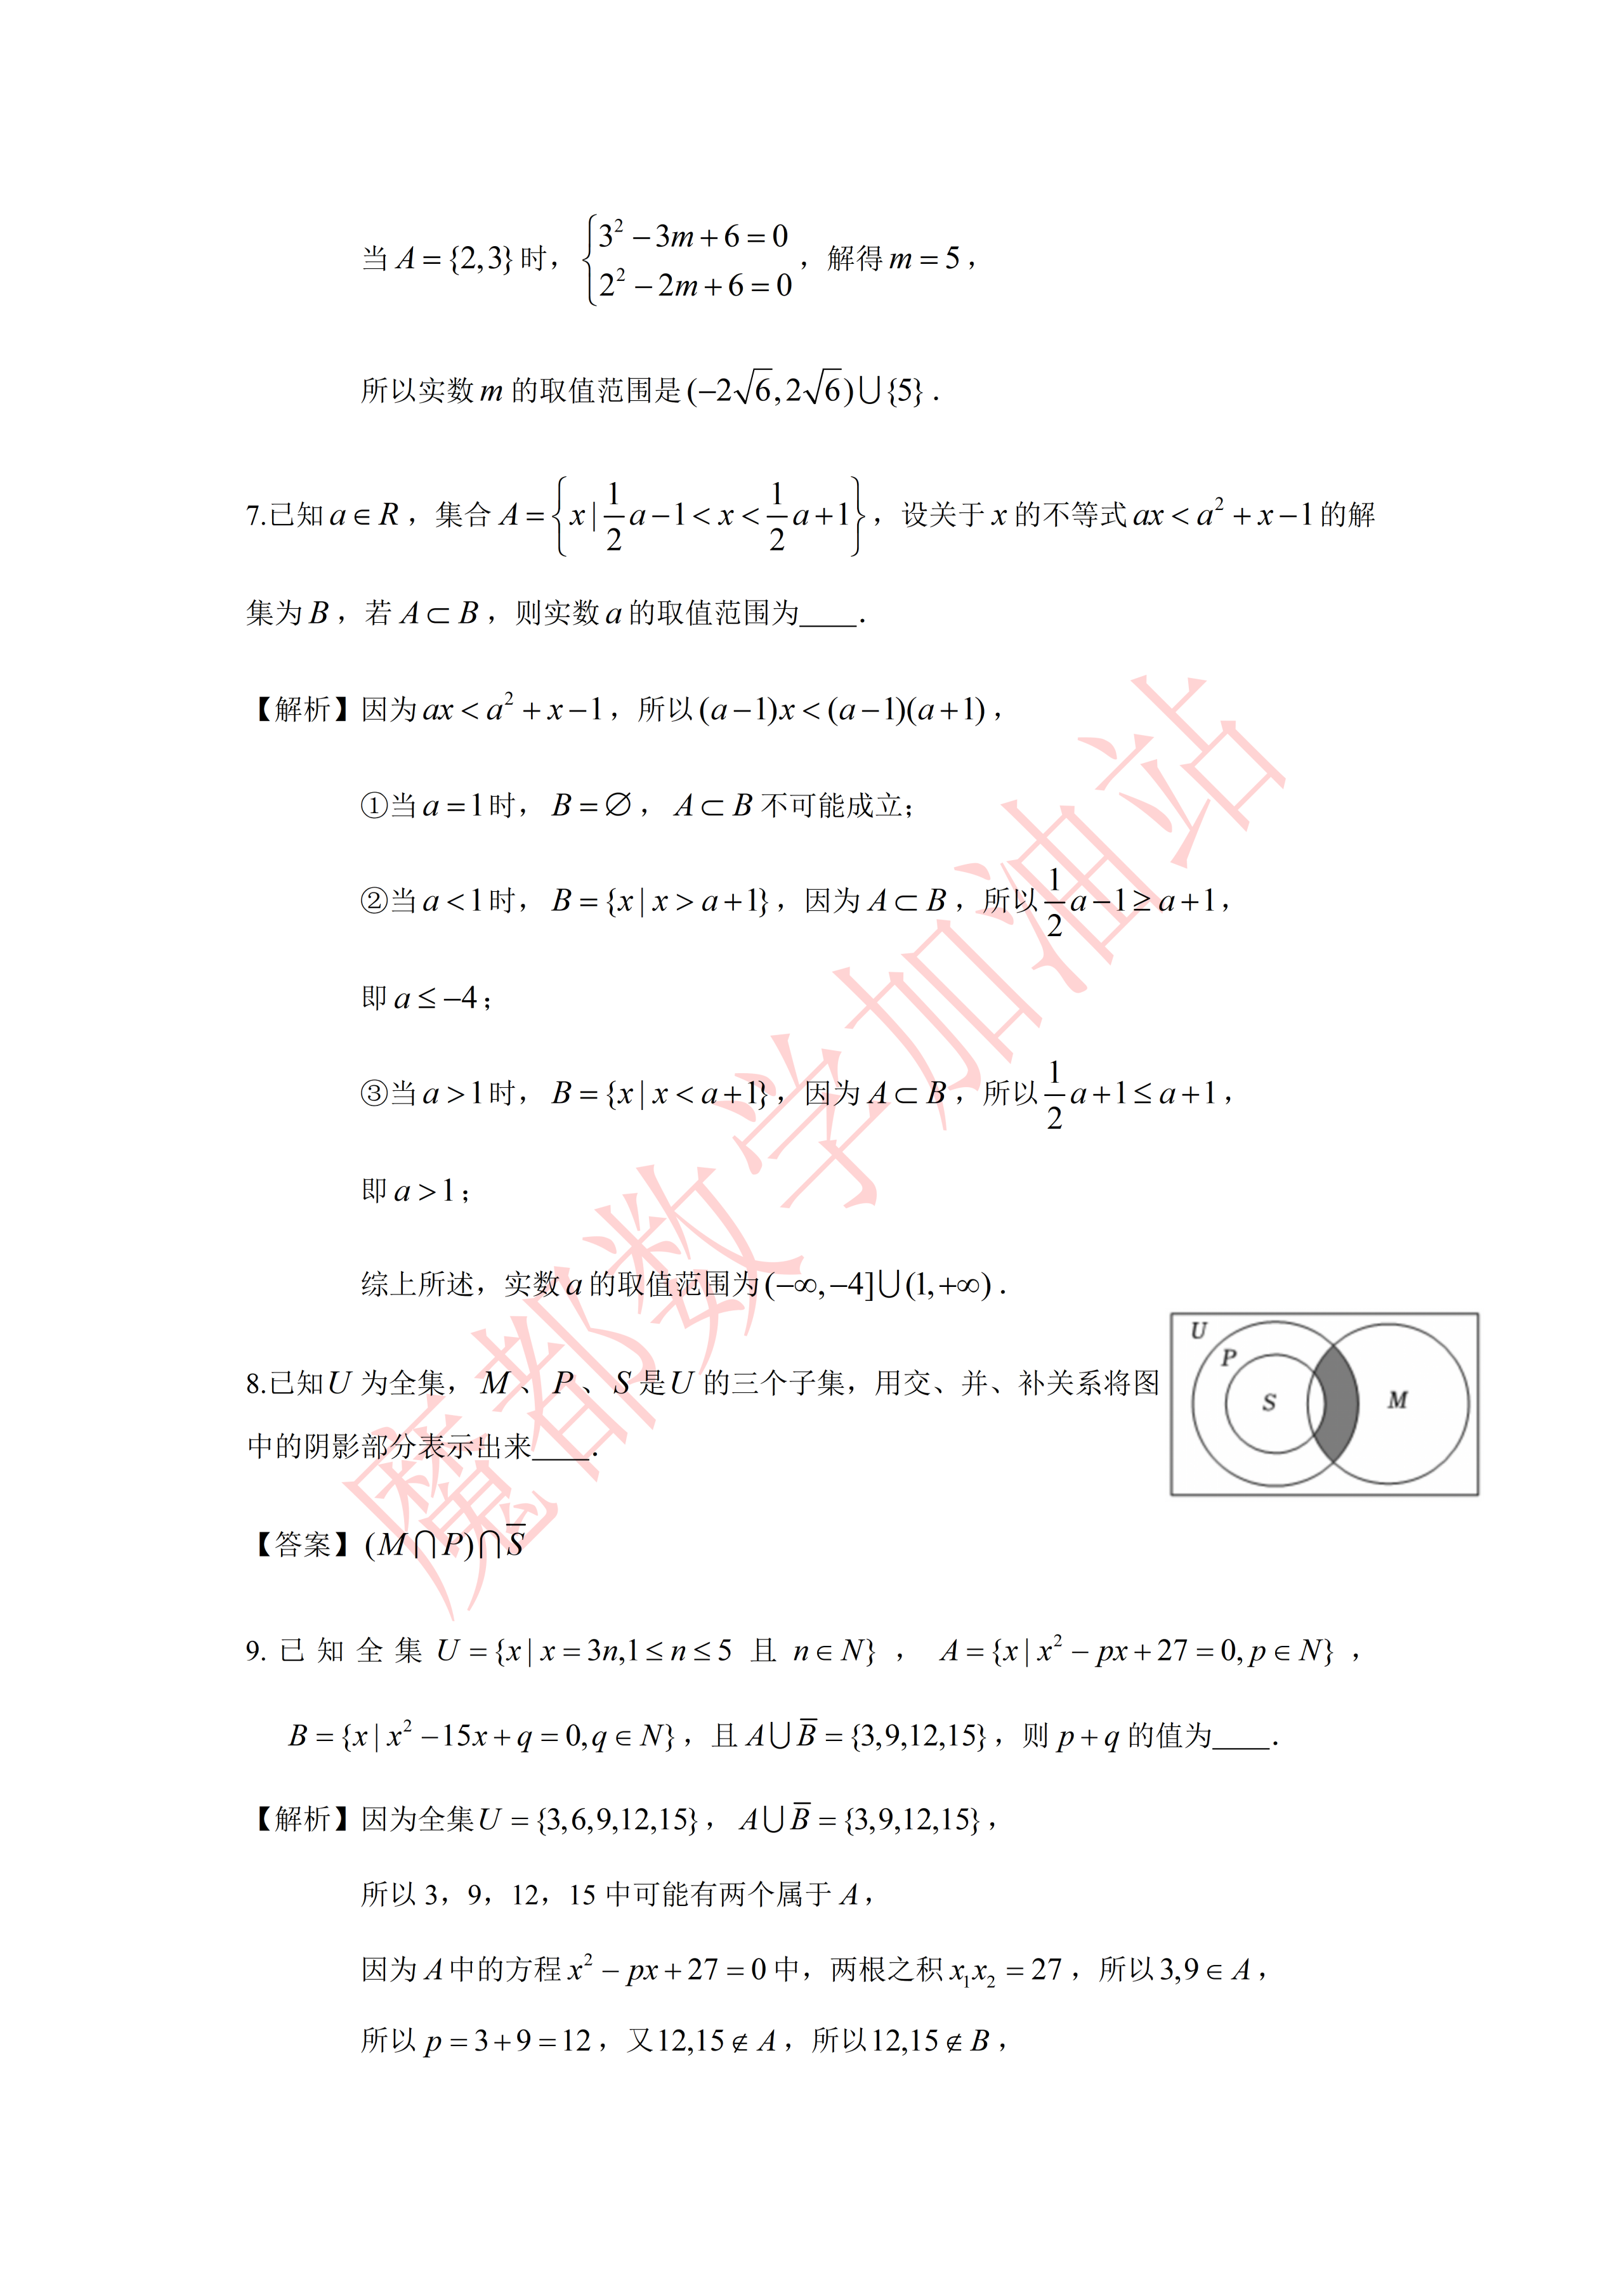
\includegraphics[width=.38\linewidth,trim=1835bp 1255bp 220bp 1565bp,clip]{../原图/高一49_华师大二附中_国庆作业1/02.png}
\end{center}

\ifanswer
\ans{$(M\cap P)\cap\overline S$}
\fi

\item 已知全集 $U=\{x\mid x=3n,1\leqslant n\leqslant5\text{ 且 }n\in\N\}$，$A=\{x\mid x^2-px+27=0,p\in\N\}$，$B=\{x\mid x^2-15x+q=0,q\in\N\}$，且 $A\cup\overline B=\{3,9,12,15\}$，则 $p+q$ 的值为\blankline[4.4em].

\ifanswer
\solbegin
\step{因为全集 $U=\{3,6,9,12,15\}$，$A\cup\overline B=\{3,9,12,15\}$，}
\step{所以 $3$、$9$、$12$、$15$ 中可能有两个属于 $A$，}
\step{因为 $A$ 中的方程 $x^2-px+27=0$ 中，两根之积 $x_1x_2=27$，所以 $3,9\in A$，}
\step{所以 $p=3+9=12$，又 $12,15\notin A$，所以 $12,15\notin B$，}
\step{因为 $B$ 中的方程 $x^2-15x+q=0$ 中，两根之和 $x_3+x_4=15$，所以 $6,9\in B$，}
\step{则 $q=6\times9=54$，所以 $p+q=66$.}
\solend
\fi

\item 已知集合 $A=\{x\mid x^2+(2a-3)x-3a=0,a\in\R,x\in\R\}$，集合 $B=\{x\mid x^2+(a-3)x+a^2-3a=0,a\in\R,x\in\R\}$，若 $A\neq B$，$A\cap B\neq\varnothing$，则 $A\cup B=$\blankline[4.4em].

\ifanswer
\solbegin
\step{设两个集合中的方程的公共解是 $b$，}
\step{由 $b^2+(2a-3)b-3a=b^2+(a-3)b+a^2-3a$，得 $ab=a^2$，}
\step{则 $a=0$ 或 $b=a$，}
\step{当 $a=0$ 时，不合题意，}
\step{当 $b=a$ 时，即两个方程的公共解为 $b=a$，}
\step{将 $b=a$ 代入方程，得 $a^2=2a$，$a=2$，}
\step{所以 $A=\{2,-3\}$，$B=\{-1,2\}$，所以 $A\cup B=\{-1,2,-3\}$.}
\solend
\fi

\item 已知一个有四个数字元素的集合 $S$，$S$ 的所有子集的元素和（空集的元素和认为是 $0$）的总和为 $16192$，则 $S$ 的元素之和等于\blankline[4.4em].

\ifanswer
\solbegin
\step{设 $S=\{a_1,a_2,a_3,a_4\}$，$S$ 的每个元素在所有子集中均出现 $2^3$ 次，}
\step{故 $(a_1+a_2+a_3+a_4)\cdot2^3=16192$，所以 $a_1+a_2+a_3+a_4=2024$，}
\step{故 $S$ 的元素之和等于 $2024$.}
\solend
\fi

\item 设 $P$ 为非空实数集满足：对任意给定的 $x,y\in P$（$x$、$y$ 可以相同），都有 $x+y\in P,x-y\in P,xy\in P$，则称 $P$ 为封闭集．关于封闭集有下列结论：

①集合 $P=\{-2,-1,0,1,2\}$ 为封闭集；

②集合 $P=\{x\mid x=2n,n\in\Z\}$ 为封闭集；

③若集合 $P_1$、$P_2$ 为封闭集，则 $P_1\cup P_2$ 为封闭集；

④若集合 $P$ 为封闭集，则一定有 $0\in P$；

⑤若集合 $P_1$、$P_2$ 为封闭集，则 $P_1\cap P_2$ 为封闭集.

其中正确结论的序号是\blankline[4.4em].

\ifanswer
\solbegin
\step{对于集合 $P=\{-2,-1,0,1,2\}$，取 $x=2$，$y=-2$，则 $x-y=2-(-2)=4\notin P$，}
\step{不满足封闭集的定义，所以①错误.}
\step{对于集合 $P=\{x\mid x=2n,n\in\Z\}$，设 $x=2n_1$，$y=2n_2$，$n_1,n_2\in\Z$.}
\step{$x+y=2n_1+2n_2=2(n_1+n_2)$，因为 $n_1+n_2\in\Z$，所以 $x+y\in P$.}
\step{$x-y=2n_1-2n_2=2(n_1-n_2)$，因为 $n_1-n_2\in\Z$，所以 $x-y\in P$.}
\step{$xy=2n_1\times2n_2=4n_1n_2=2(2n_1n_2)$，因为 $2n_1n_2\in\Z$，所以 $xy\in P$.}
\step{满足封闭集的定义，所以②正确.}
\step{令 $P_1=\{x\mid x=2n,n\in\Z\}$，$P_2=\{x\mid x=3n,n\in\Z\}$，都是封闭集.}
\step{$P_1\cup P_2$ 中，取 $x=2(x\in P_1)$，$y=3(y\in P_2)$，$x+y=5\notin P_1\cup P_2$，}
\step{不满足封闭集的定义，所以③错误.}
\step{因为对任意 $x\in P$，有 $x-x=0\in P$，}
\step{所以若集合 $P$ 为封闭集，则一定有 $0\in P$，所以④正确.}
\step{因为 $P_1$、$P_2$ 为封闭集，设 $x,y\in P_1\cap P_2$，则 $x,y\in P_1$ 且 $x,y\in P_2$.}
\step{因为 $P_1$ 是封闭集，所以 $x+y\in P_1,x-y\in P_1,xy\in P_1$.}
\step{因为 $P_2$ 是封闭集，所以 $x+y\in P_2,x-y\in P_2,xy\in P_2$.}
\step{所以 $x+y\in P_1\cap P_2,x-y\in P_1\cap P_2,xy\in P_1\cap P_2$，满足封闭集的定义，}
\step{所以⑤正确.}
\step{故正确的是②④⑤.}
\solend
\fi

\end{enumerate}

\bigsec{二、选择题}

\begin{enumerate}
\setcounter{enumi}{12}

\item 已知集合 $A=\{1,3,\sqrt m\}$，$B=\{1,m\}$，$B\subseteq A$，则 $m=$\mbox{（\quad）}

\keepwithprev
A. $0$ 或 $\sqrt3$\qquad B. $0$ 或 $3$

C. $1$ 或 $\sqrt3$\qquad D. $1$ 或 $3$

\ifanswer
\solbegin
\step{因为集合 $A=\{1,3,\sqrt m\}$，$B=\{1,m\}$，$B\subseteq A$，所以 $m=3$ 或 $m=\sqrt m$，}
\step{若 $m=3$，$A=\{1,3,\sqrt3\}$，$B=\{1,3\}$，满足 $B\subseteq A$，}
\step{若 $m=\sqrt m$，解得 $m=1$ 或 $m=0$，}
\step{①若 $m=0$，则 $A=\{1,3,0\}$，$B=\{1,0\}$，满足 $B\subseteq A$.}
\step{②若 $m=1$，则 $A$、$B$ 不满足集合中元素的互异性，舍去.}
\step{综上，$m=0$ 或 $m=3$．故选 $B$.}
\solend
\fi

\needvspace{10\baselineskip}

\item 设集合 $A$、$B$、$C$、$D$ 是全集 $X$ 的子集，$A\cap B\neq\varnothing$，$A\cap C\neq\varnothing$，则下列选项中正确的是\mbox{（\quad）}

\keepwithprev
A. 如果 $D\subset B$ 或 $D\subset C$，则 $D\cap A\neq\varnothing$

B. 如果 $D\subset A$，则 $\overline D\cap B\neq\varnothing$，$\overline D\cap C\neq\varnothing$

C. 如果 $A\subset D$，则 $\overline D\cap B=\varnothing$，$\overline D\cap C=\varnothing$

D. 上述各项都不正确

\ifanswer
\solbegin
\step{用韦恩图表示每个选项：}
\begin{center}
% 原图第 5 页解析配图（三联韦恩图）直接裁取（原卷排于选项 C、D 右侧）。
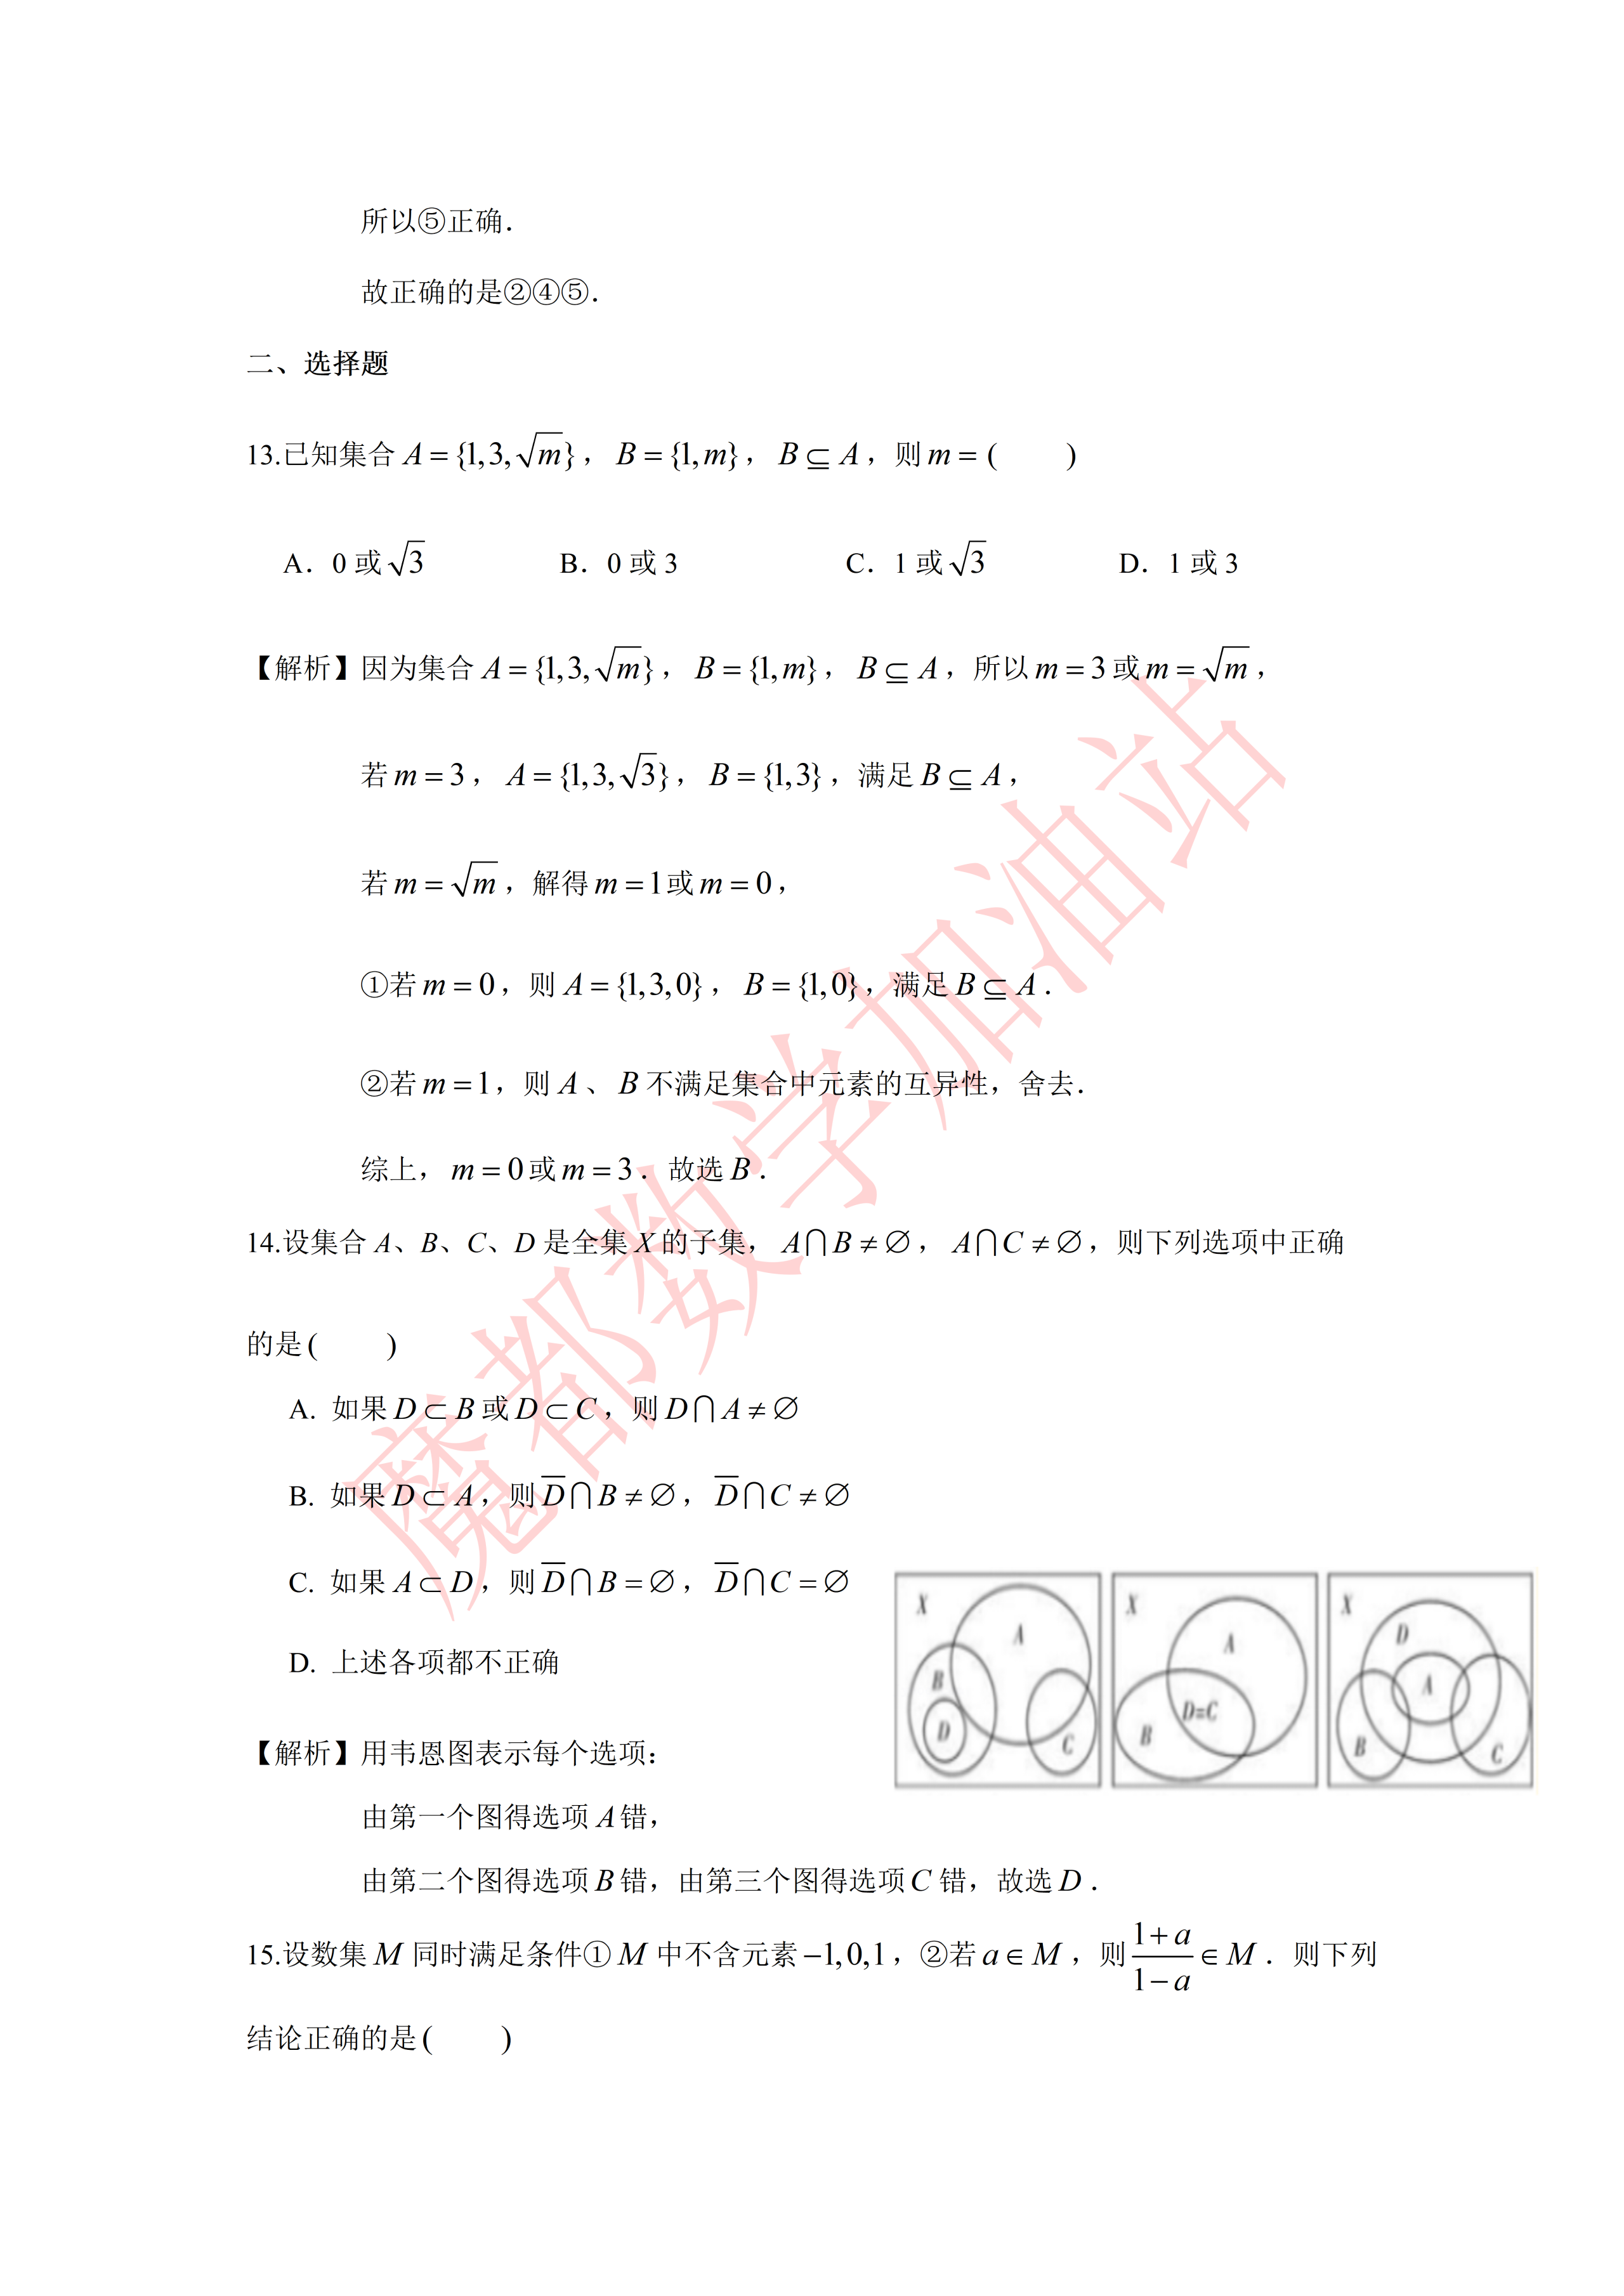
\includegraphics[width=.75\linewidth,trim=1400bp 790bp 135bp 1155bp,clip]{../原图/高一49_华师大二附中_国庆作业1/05.png}
\end{center}
\step{由第一个图得选项 $A$ 错，}
\step{由第二个图得选项 $B$ 错，由第三个图得选项 $C$ 错，故选 $D$.}
\solend
\fi

\item 设数集 $M$ 同时满足条件①$M$ 中不含元素 $-1$、$0$、$1$，②若 $a\in M$，则 $\dfrac{1+a}{1-a}\in M$．则下列结论正确的是\mbox{（\quad）}

\keepwithprev
A. 集合 $M$ 中至多有 $2$ 个元素\qquad B. 集合 $M$ 中至多有 $3$ 个元素

C. 集合 $M$ 中有且仅有 $4$ 个元素\qquad D. 集合 $M$ 中有无穷多个元素

\ifanswer
\solbegin
\step{若集合只含有一个元素，则 $\dfrac{1+a}{1-a}=a$，即 $1+a=a-a^2$，即 $-a^2=1$，不成立.}
\step{当 $a=3$ 时，$\dfrac{1+3}{1-3}=-2\in M$，所以 $\dfrac{1-2}{1+2}=-\dfrac13\in M$，所以 $\dfrac{1-\frac13}{1+\frac13}=\dfrac12\in M$，}
\step{所以 $\dfrac{1+\frac12}{1-\frac12}=3$，开始重复了，所以 $M=\left\{3,-2,-\dfrac13,\dfrac12\right\}$；}
\step{当 $a=2$ 时，$\dfrac{1+2}{1-2}=-3\in M$，所以 $\dfrac{1-3}{1+3}=-\dfrac12\in M$，所以 $\dfrac{1-\frac12}{1+\frac12}=\dfrac13\in M$，}
\step{所以 $\dfrac{1+\frac13}{1-\frac13}=2$，开始重复了，所以 $M=\left\{2,-3,-\dfrac12,-\dfrac13\right\}$，}
\step{此时也只要四个元素；}
\step{当 $a=\dfrac34\in M$，则 $7\in M$，若 $7\in M$，则 $-\dfrac43\in M$，}
\step{若 $-\dfrac43\in M$，则 $-\dfrac17\in M$，若 $-\dfrac17\in M$，有 $\dfrac34\in M$，}
\step{由归纳推理得，集合 $M$ 中有且仅有 $4$ 个元素．故选 $C$.}
\solend
\fi

\item 已知集合 $M=\{x\mid x\in\N,0<x\leqslant15\}$，$A_1$、$A_2$、$A_3$ 满足：①$A_1\cup A_2\cup A_3=M$；②每个集合都恰有 $5$ 个元素．集合 $A_i$（$i=1,2,3$）中最大元素与最小元素之和称为 $A_i$ 的特征数，记为 $X_i$（$i=1,2,3$），则 $X_1+X_2+X_3$ 的值不可能为\mbox{（\quad）}

\keepwithprev
A. $37$\qquad B. $39$\qquad C. $48$\qquad D. $57$

\ifanswer
\solbegin
\step{因为集合 $M=\{x\mid x\in\N,0<x\leqslant15\}=\{1,2,3,\cdots,15\}$，}
\step{又因为集合 $A_1$、$A_2$、$A_3$ 中，每个集合恰有 $5$ 个元素，}
\step{且 $A_1\cup A_2\cup A_3=M$ 有 $15$ 个元素，所以集合 $A_1$、$A_2$、$A_3$ 中没有重复元素，}
\step{因为 $1$ 是集合 $M$ 中数值最小的元素，$15$ 是集合 $M$ 中数值最大的元素，}
\step{所以在 $A_i$ 的特征数构成中，必有 $1$ 和 $15$，不妨设 $1\in A_1$，$15\in A_1$，}
\step{要使 $X_1+X_2+X_3$ 最大，则应该在集合 $A_1$ 中首先放置数值较小的元素，}
\step{即 $A_1=\{1,2,3,4,15\}$，所以 $5$ 与 $14$ 是剩下元素中数值最小或最大的元素，}
\step{同理，不妨设 $5\in A_2$，$14\in A_2$，接着在 $A_2$ 中再次放置数值较小的元素，}
\step{即 $A_2=\{5,6,7,8,14\}$，则 $A_3=\{9,10,11,12,13\}$，}
\step{此时 $X_1+X_2+X_3$ 有最大值为 $1+15+5+14+9+13=57$，}
\step{即 $X_1+X_2+X_3\leqslant57$；}
\step{要使 $X_1+X_2+X_3$ 最小，则在集合 $A_1$ 中首先放置数值较大的元素，}
\step{即 $A_1=\{1,12,13,14,15\}$，所以 $2$ 与 $11$ 是剩下元素中数值最小或最大的元素，}
\step{同理，不妨设 $2\in A_2$，$11\in A_2$，接着在 $A_2$ 中再次放置数值较大的元素，}
\step{即 $A_2=\{2,8,9,10,11\}$，则 $A_3=\{3,4,5,6,7\}$，}
\step{此时 $X_1+X_2+X_3$ 有最小值为 $1+15+2+11+3+7=39$，}
\step{即 $X_1+X_2+X_3\geqslant39$，}
\step{综上，$39\leqslant X_1+X_2+X_3\leqslant57$，故选 $A$.}
\solend
\fi

\end{enumerate}

\bigsec{三、解答题}

\begin{enumerate}
\setcounter{enumi}{16}

\item 已知全集为 $\R$，集合 $A=\{x\mid y=\sqrt{(2+x)(4-x)}\}$，$B=\{x\mid-1<x<m+1\}$.

\begin{enumerate}[label=(\arabic*)]
\item 若 $m=4$，求 $A\cup B$、$\overline A\cap B$；
\item 若 $B\subseteq A$，求实数 $m$ 的取值范围.
\end{enumerate}

\ifanswer
\solbegin
\stepm{(1)}{集合 $A=\{x\mid y=\sqrt{(2+x)(4-x)}\}=\{x\mid-2\leqslant x\leqslant4\}$，}
\step{当 $m=4$ 时，$B=\{x\mid-1<x<5\}$.}
\step{所以 $A\cup B=[-2,5)$，$\overline A=\{x\mid x<-2\text{ 或 }x>4\}$，$\overline A\cap B=(4,5)$.}
\stepm{(2)}{因为 $B\subseteq A$，}
% 原卷如此，照录未改（第 17 题(2)解析两处"当 C=∅／当 C≠∅"应为 B，本卷并无集合 C）
\step{当 $C=\varnothing$ 时，$m\leqslant-2$，$B\subseteq A$ 成立；}
\step{当 $C\neq\varnothing$ 时，$m>-2$，$-1<m+1\leqslant4$，解得 $-2<m\leqslant3$，}
\step{综上，$m\leqslant3$，所以实数 $m$ 的取值范围是 $(-\infty,3]$.}
\solend
\fi

\ansspace[6]

\item 用反证法证明：若 $a$、$b$、$c\in\R$，且 $x=a^2-2b+1$，$y=b^2-2c+1$，$z=c^2-2a+1$，则 $x$、$y$、$z$ 中至少有一个不小于 $0$.

\ifanswer
\solbegin
\step{假设 $x$、$y$、$z$ 均小于 $0$，即 $x=a^2-2b+1<0$①，$y=b^2-2c+1<0$②，}
\step{$z=c^2-2a+1<0$③，①$+$②$+$③得 $x+y+z=(a-1)^2+(b-1)^2+(c-1)^2<0$，}
\step{这与 $(a-1)^2+(b-1)^2+(c-1)^2\geqslant0$ 矛盾，则假设不成立，}
\step{所以 $x$、$y$、$z$ 中至少有一个不小于 $0$，得证.}
\solend
\fi

\ansspace[5]

\item 已知全集为 $\R$，实数 $a$、$b$ 满足 $a\neq b$，集合 $M=\{x\mid x^2-3x-4\leqslant0\}$，集合 $A=\{x\mid(x+a)(x+b)>0\}$，集合 $B=\{x\mid x^2+(a-2)x-2a>0\}$.

\begin{enumerate}[label=(\arabic*)]
\item 若 $\overline A=M$，求 $a$、$b$ 的值；
\item 若 $a>b>-1$，求 $A\cap B$；
\item 若 $a^2+a\in\overline B$，求 $a$ 的取值范围.
\end{enumerate}

\ifanswer
\solbegin
\stepm{(1)}{$M=\{x\mid x^2-3x-4\leqslant0\}=\{x\mid-1\leqslant x\leqslant4\}$，$A=\{x\mid(x+a)(x+b)\leqslant0\}$，}
\step{因为 $\overline A=M$，所以 $a=1$，$b=-4$ 或 $a=-4$，$b=1$.}
\stepm{(2)}{因为 $a>b>-1$，所以 $-a<-b<1$，所以 $A=\{x\mid x<-a\text{ 或 }x>-b\}$，}
\step{因为 $B=\{x\mid x^2+(a-2)x-2a>0\}=\{x\mid x<-a\text{ 或 }x>2\}$，}
\step{所以 $A\cap B=\{x\mid x<-a\text{ 或 }x>2\}$，}
\stepm{(3)}{$\overline B=\{x\mid(x-2)(x+a)\leqslant0\}$，}
% 原卷如此，照录未改（第 19 题(3)此处"a(a-1)((a-2)^2≤0"括号不配对；且由左式展开应为
% a(a-1)(a+2)^2≤0，与下句"解得 a=2 …[0,1]∪{2}"按 (a-2)^2 方自洽，见文件头清单第 2 条）
\step{由 $a^2+a\in\overline B$，得 $(a^2+a-2)(a^2+2a)\leqslant0\Leftrightarrow a(a-1)((a-2)^2\leqslant0$，}
\step{解得 $a=2$ 或 $0\leqslant a\leqslant1$，故 $a$ 的取值范围是 $[0,1]\cup\{2\}$.}
\solend
\fi

\ansspace[7]

\item 设数集 $A$ 由实数构成，若 $x\in A$（$x\neq1$ 且 $x\neq0$），则 $\dfrac{1}{1-x}\in A$.

\begin{enumerate}[label=(\arabic*)]
\item 若 $2\in A$，则 $A$ 中至少还有几个元素；
\item 集合 $A$ 是否为双元素集合？请说明理由；
\item 若 $A$ 中元素个数不超过 $8$ 个，所有元素的和为 $\dfrac{14}{3}$，且 $A$ 中有一个元素的平方等于所有元素的积，求集合 $A$.
\end{enumerate}

\ifanswer
\solbegin
\stepm{(1)}{若 $x\in A$，则 $\dfrac{1}{1-x}\in A$，又 $2\in A$，所以 $\dfrac{1}{1-2}=-1\in A$，}
\step{所以 $\dfrac{1}{1-(-1)}=\dfrac12\in A$，所以 $\dfrac{1}{1-\frac12}=2\in A$，}
% 原卷如此，照录未改（第 20 题(1)解析末句"2 个几个元素"衍一"几个"）
\step{所以 $A$ 中至少还有 $2$ 个几个元素；}
\stepm{(2)}{若 $x\in A$（$x\neq1$ 且 $x\neq0$），则 $\dfrac{1}{1-x}\in A$，}
\step{则 $\dfrac{1}{1-\frac{1}{1-x}}=\dfrac{1-x}{-x}\in A$，则 $\dfrac{1}{1-\frac{1-x}{-x}}=x\in A$}
\step{若 $A$ 为双元素集，则 $x=\dfrac{1}{1-x}$ 或 $x=\dfrac{1-x}{-x}$ 或 $\dfrac{1}{1-x}=\dfrac{1-x}{-x}$，均无解，}
\step{所以 $A$ 不可能为双元素集；}
\stepm{(3)}{由 $x\in A$，$\dfrac{1}{1-x}\in A$，得 $\dfrac{1}{1-\frac{1}{1-x}}=\dfrac{x-1}{x}\in A$，得 $\dfrac{1}{1-\frac{x-1}{x}}=x\in A$，}
\step{所以 $\left\{x,\dfrac{1}{1-x},\dfrac{x-1}{x}\right\}\subseteq A$，而 $x\cdot\dfrac{1}{1-x}\cdot\dfrac{x-1}{x}=-1$，}
\step{$A$ 中元素个数为 $3$ 的倍数，则 $A$ 中元素只有 $6$ 个，}
\step{因为 $A$ 中有一个元素的平方等于所有元素的积，}
\step{不妨设 $x^2=1$，解得 $x=-1$ 或 $x=1$（舍），则 $-1$、$\dfrac12$、$2\in A$，}
\step{所以 $-1+\dfrac12+2+m+\dfrac{1}{1-m}+\dfrac{m-1}{m}=\dfrac{14}{3}$，解得 $m=-\dfrac12$ 或 $m=3$ 或 $m=\dfrac23$，}
\step{所以 $A=\left\{\dfrac12,2,-1,-\dfrac12,3,\dfrac23\right\}$.}
\solend
\fi

\ansspace[9]

% 原卷如此，照录未改（第 21 题题干"21.求已知集合"之"求"字疑衍；"任意两个元素 a_i a_j"
% 疑脱逗号；"|a_i-a_j|≥1/30 则称"之前疑脱标点，见文件头清单第 4 条）
\item 求已知集合 $M=\left\{\dfrac{1}{k}\middle|1\leqslant k\leqslant100\text{ 且 }k\in\N^{*}\right\}$，$A=\{a_1,a_2,\cdots,a_n\}$，其中 $n\in\N^{*}$，且 $n\geqslant2$．若 $A\subseteq\N$，且对集合 $A$ 中的任意两个元素 $a_ia_j$，$i\neq j$ 都有 $|a_i-a_j|\geqslant\dfrac{1}{30}$ 则称集合 $A$ 有性质 $P$.

\begin{enumerate}[label=(\arabic*)]
\item 判断集合 $\left\{\dfrac13,\dfrac14,\dfrac15,\dfrac16,\dfrac17\right\}$ 是否具有性质 $P$；
\item 若集合 $A=\{a_1,a_2,\cdots,a_n\}$ 具有性质 $P$.

①求证：$a_i-a_j$ 的最大值大于等于 $\dfrac{n-1}{30}$；

②求 $A$ 的元素个数 $n$ 的最大值.
\end{enumerate}

\ifanswer
\solbegin
\stepm{(1)}{集合为 $\left\{\dfrac13,\dfrac14,\dfrac15,\dfrac16,\dfrac17\right\}$，又 $\dfrac16-\dfrac17=\dfrac{1}{42}<\dfrac{1}{30}$，所以该集合不具有性质 $P$；}
\stepm{(2)}{①因为集合 $A=\{a_1,a_2,\cdots,a_n\}$ 具有性质 $P$，}
\step{不妨设 $a_1<a_2<a_3<\cdots<a_n$，则 $a_i-a_j\geqslant\dfrac{1}{30}$（$i>j$），}
\step{所以 $a_n-a_1=(a_n-a_{n-1})+(a_{n-1}-a_{n-2})+\cdots+(a_2-a_1)\geqslant\dfrac{n-1}{30}$，}
\step{故 $a_i-a_j$ 的最大值大于等于 $\dfrac{n-1}{30}$；}
% 原卷如此，照录未改（第 21 题(2)②首行"a_2-a_1≥(n-1)/30"：由①同款推理只能得
% a_2-a_1≥1/30，见文件头清单第 5 条）
\step{②$A=\{a_1,a_2,\cdots,a_n\}$，不妨设 $a_1<a_2<a_3<\cdots<a_n$，}
\step{要使 $A$ 的元素个数 $n$ 最大，}
\step{则 $A$ 中的元素满足 $a_n=\dfrac{1}{k}$，$a_{n-1}=\dfrac{1}{k+1}$，$\cdots$，$a_1=\dfrac{1}{k+n-1}$（$k\in\N^{*}$），}
\step{又由①得 $a_2-a_1=\dfrac{1}{k+n-2}-\dfrac{1}{k+n-1}\geqslant\dfrac{n-1}{30}$，}
\step{所以 $(k+n-2)(k+n-1)\leqslant30$，又 $a_n-a_{n-1}=\dfrac{1}{k}-\dfrac{1}{k+1}\geqslant\dfrac{1}{30}$，}
\step{所以 $k(k+1)\leqslant30$，所以 $1\leqslant k\leqslant5$（$k\in\N^{*}$），}
\step{当 $k=5$ 时，由 $(k+n-2)(k+n-1)\leqslant30$，解得 $n\leqslant2$，$n\in\N^{*}$；}
\step{当 $k=4$ 时，由 $(k+n-2)(k+n-1)\leqslant30$，解得 $n\leqslant3$，$n\in\N^{*}$；}
\step{当 $k=3$ 时，由 $(k+n-2)(k+n-1)\leqslant30$，解得 $n\leqslant4$，$n\in\N^{*}$；}
\step{当 $k=2$ 时，由 $(k+n-2)(k+n-1)\leqslant30$，解得 $n\leqslant5$，$n\in\N^{*}$；}
\step{当 $k=1$ 时，由 $(k+n-2)(k+n-1)\leqslant30$，解得 $n\leqslant6$，$n\in\N^{*}$.}
\step{故 $A$ 的元素个数 $n$ 的最大值为 $6$，此时集合 $A=\left\{1,\dfrac12,\dfrac13,\cdots,\dfrac16\right\}$.}
\solend
\fi

\ansspace*[10]

\end{enumerate}

\end{document}
"
%
% 原始材料：微信公众号"魔都数学加油站"文章，作者破晓，连载"27学年高一49"；
% 原文标题"27学年高一49——2026-2027年上海市华师大二附中高一上国庆作业1集合与逻辑、
% 等式与不等式的性质"；页面用 JS 渲染，未见明确发布日期（页内时间戳 ≈ 2026-10-05 21:37）；
% 原文链接：https://mp.weixin.qq.com/s/XxZTOBVQslK5cZm2_BbhOg。
% 正文为 11 张 PNG 页：第 01、03、04、06、07、08、09 页 4762×6735，
% 第 02、05、10、11 页 2560×3620，均按页序读取；粉色斜排"魔都数学加油站"为卷面水印，
% 与公众号页脚一并未录入。全卷 11 页均为试卷页，无二维码/宣传页。
%
% 题号与分节：原文自第 3 题起编，填空题 3—12、选择题 13—16、解答题 17—21，共 19 题。
% 讲评版：原卷每题下直接印【答案】或【解析】——只印【答案】的 3 题（第 3、5、8 题），
% 其余 16 题均只印【解析】；解析行数已逐题按印刷行照录（一条 \step＝原卷一个印刷行）。
%
% 卷首标题：照卷面印作"2026-2027 年华师大二附中高一上国庆作业 1"（公众号标题中的"上海市"
% 卷面没有，本稿照卷面），年份区间按全稿惯例排 en dash；副标题照卷面自印的
% "集合与逻辑单元综合检测"（原卷页首标题行下方即印此行，故不另按模块口径拟名）。
% 副标题依据：全卷 19 题均为集合与常用逻辑用语内容——集合类 15 题（6—17、19—21 中除
% 反证法题外），逻辑/命题类 3 题（第 3 题否定形式、第 4 题充要条件、第 5 题反证法假设），
% 反证法证明 1 题（第 18 题）；全卷无不等式求解题，公众号标题中"等式与不等式的性质"
% 与卷面实际内容不符。
%
% 与原卷的排版差异：
%   ① 原文从第 3 题起，填空题为 3—12、选择题为 13—16、解答题为 17—21，本稿保留原题号；
%   ② 原卷每题下直接印【答案】/【解析】，本稿按全稿惯例置于答案版；只印【解析】的题
%      不另提 \ans{}（照 高一36 口径），只印【答案】的题仅给 \ans{}；
%   ③ 原卷第 8 题韦恩图排在题干右侧、第 14 题三联韦恩图排在选项（C、D）右侧，
%      本稿分别移至题干下方、解析首步之后居中排，均直接裁取原图页（02.png、05.png）；
%   ④ 数集记号原卷排作斜体/加粗 R、N、Z，本稿统一为 \R、\N、\Z、\N^*；
%      填空横线按全稿惯例排为 \blankline[4.4em]。
%
% 原卷笔误/存疑清单（均照录未改，正文中该处有 % 注）：
%   1. 第 17 题(2)解析两处"当 C=∅／当 C≠∅"应为 B（本卷并无集合 C）；
%   2. 第 19 题(3)解析"a(a-1)((a-2)^2≤0"括号不配对（多一枚左括号）；且由
%      (a^2+a-2)(a^2+2a)≤0 展开应为 a(a-1)(a+2)^2≤0，与原卷结论"解得 a=2 …
%      [0,1]∪{2}"恰按 (a-2)^2 自洽——因式分解与原式不符，结论按 (a-2)^2 自洽，均照录；
%   3. 第 20 题(1)解析末句"至少还有 2 个几个元素"衍一"几个"；
%   4. 第 21 题题干"21.求已知集合"之"求"字疑衍；"任意两个元素 a_i a_j"疑脱逗号；
%      "≥1/30 则称"之前疑脱标点；
%   5. 第 21 题(2)②解析"a_2-a_1≥(n-1)/30"：由①同款推理只能得 a_2-a_1≥1/30，
%      原卷如此，照录未改（后续 (k+n-2)(k+n-1)≤30 即按该行推得）。
%
\documentclass[a4paper,11pt]{article}
\usepackage{common}

\begin{document}

\examtitlest[3]{2026--2027 年华师大二附中高一上国庆作业 1}{集合与逻辑单元综合检测}

\bigsec{一、填空题}

\begin{enumerate}
\setcounter{enumi}{2}

\item “若 $x^2-x-2\leqslant0$，则 $-1\leqslant x\leqslant2$”的否定形式为\blankline[4.4em].

\ifanswer
\ans{若 $x^2-x-2>0$，则 $x<-1$ 或 $x>2$}
\fi

\item 已知 $p:|x-3|<5$，$q:1-a<x<2a-3$，且 $p$ 是 $q$ 的充分非必要条件，则实数 $a$ 的取值范围是\blankline[4.4em].

\ifanswer
\solbegin
\step{由 $|x-3|<5$ 得 $-2<x<8$，}
\step{又 $p$ 是 $q$ 的充分不必要条件，所以 $(-2,8)\subset(1-a,2a-3)$，}
\step{即 $\begin{cases}-2\geqslant1-a\\ 8\leqslant2a-3\\ (2a-3)-(1-a)\neq8-(-2)\end{cases}$，解得 $a\geqslant\dfrac{11}{2}$，实数 $a$ 的取值范围是 $\left[\dfrac{11}{2},+\infty\right)$.}
\solend
\fi

\item 用反证法证明命题“设 $a$、$b\in\R$，则方程 $a_1x^2+b_1x+c_1=0$ 与 $a_2x^2+b_2x+c_2=0$ 至少有一个实根”时要做的假设是\blankline[4.4em].

\ifanswer
\ans{假设 $a$、$b\in\R$，方程 $a_1x^2+b_1x+c_1=0$ 与 $a_2x^2+b_2x+c_2=0$ 都没有实根}
\fi

\item 设集合 $A=\{x\mid x^2-mx+6=0,x\in\R\}$，且 $A\cap\{2,3\}=A$，则实数 $m$ 的取值范围是\blankline[4.4em].

\ifanswer
\solbegin
\step{由 $A\cap\{2,3\}=A$，得 $A\subseteq\{2,3\}$，}
\step{当 $A=\varnothing$ 时，$\Delta=m^2-24<0$，解得 $-2\sqrt6<m<2\sqrt6$；}
\step{当 $A=\{2\}$ 时，$\begin{cases}2^2-2m+6=0\\ \Delta=m^2-24=0\end{cases}$，无解；}
\step{当 $A=\{3\}$ 时，$\begin{cases}3^2-3m+6=0\\ \Delta=m^2-24=0\end{cases}$，无解；}
\step{当 $A=\{2,3\}$ 时，$\begin{cases}3^2-3m+6=0\\ 2^2-2m+6=0\end{cases}$，解得 $m=5$，}
\step{所以实数 $m$ 的取值范围是 $(-2\sqrt6,2\sqrt6)\cup\{5\}$.}
\solend
\fi

\item 已知 $a\in\R$，集合 $A=\left\{x\middle|\dfrac12a-1<x<\dfrac12a+1\right\}$，设关于 $x$ 的不等式 $ax<a^2+x-1$ 的解集为 $B$，若 $A\subset B$，则实数 $a$ 的取值范围为\blankline[4.4em].

\ifanswer
\solbegin
\step{因为 $ax<a^2+x-1$，所以 $(a-1)x<(a-1)(a+1)$，}
\step{①当 $a=1$ 时，$B=\varnothing$，$A\subset B$ 不可能成立；}
\step{②当 $a<1$ 时，$B=\{x\mid x>a+1\}$，因为 $A\subset B$，所以 $\dfrac12a-1\geqslant a+1$，}
\step{即 $a\leqslant-4$；}
\step{③当 $a>1$ 时，$B=\{x\mid x<a+1\}$，因为 $A\subset B$，所以 $\dfrac12a+1\leqslant a+1$，}
\step{即 $a>1$；}
\step{综上所述，实数 $a$ 的取值范围为 $(-\infty,-4]\cup(1,+\infty)$.}
\solend
\fi

\needvspace{8\baselineskip}

\item 已知 $U$ 为全集，$M$、$P$、$S$ 是 $U$ 的三个子集，用交、并、补关系将图中的阴影部分表示出来\blankline[4.4em].

\begin{center}
% 原图第 2 页题旁韦恩图直接裁取（原卷排于题干右侧）。
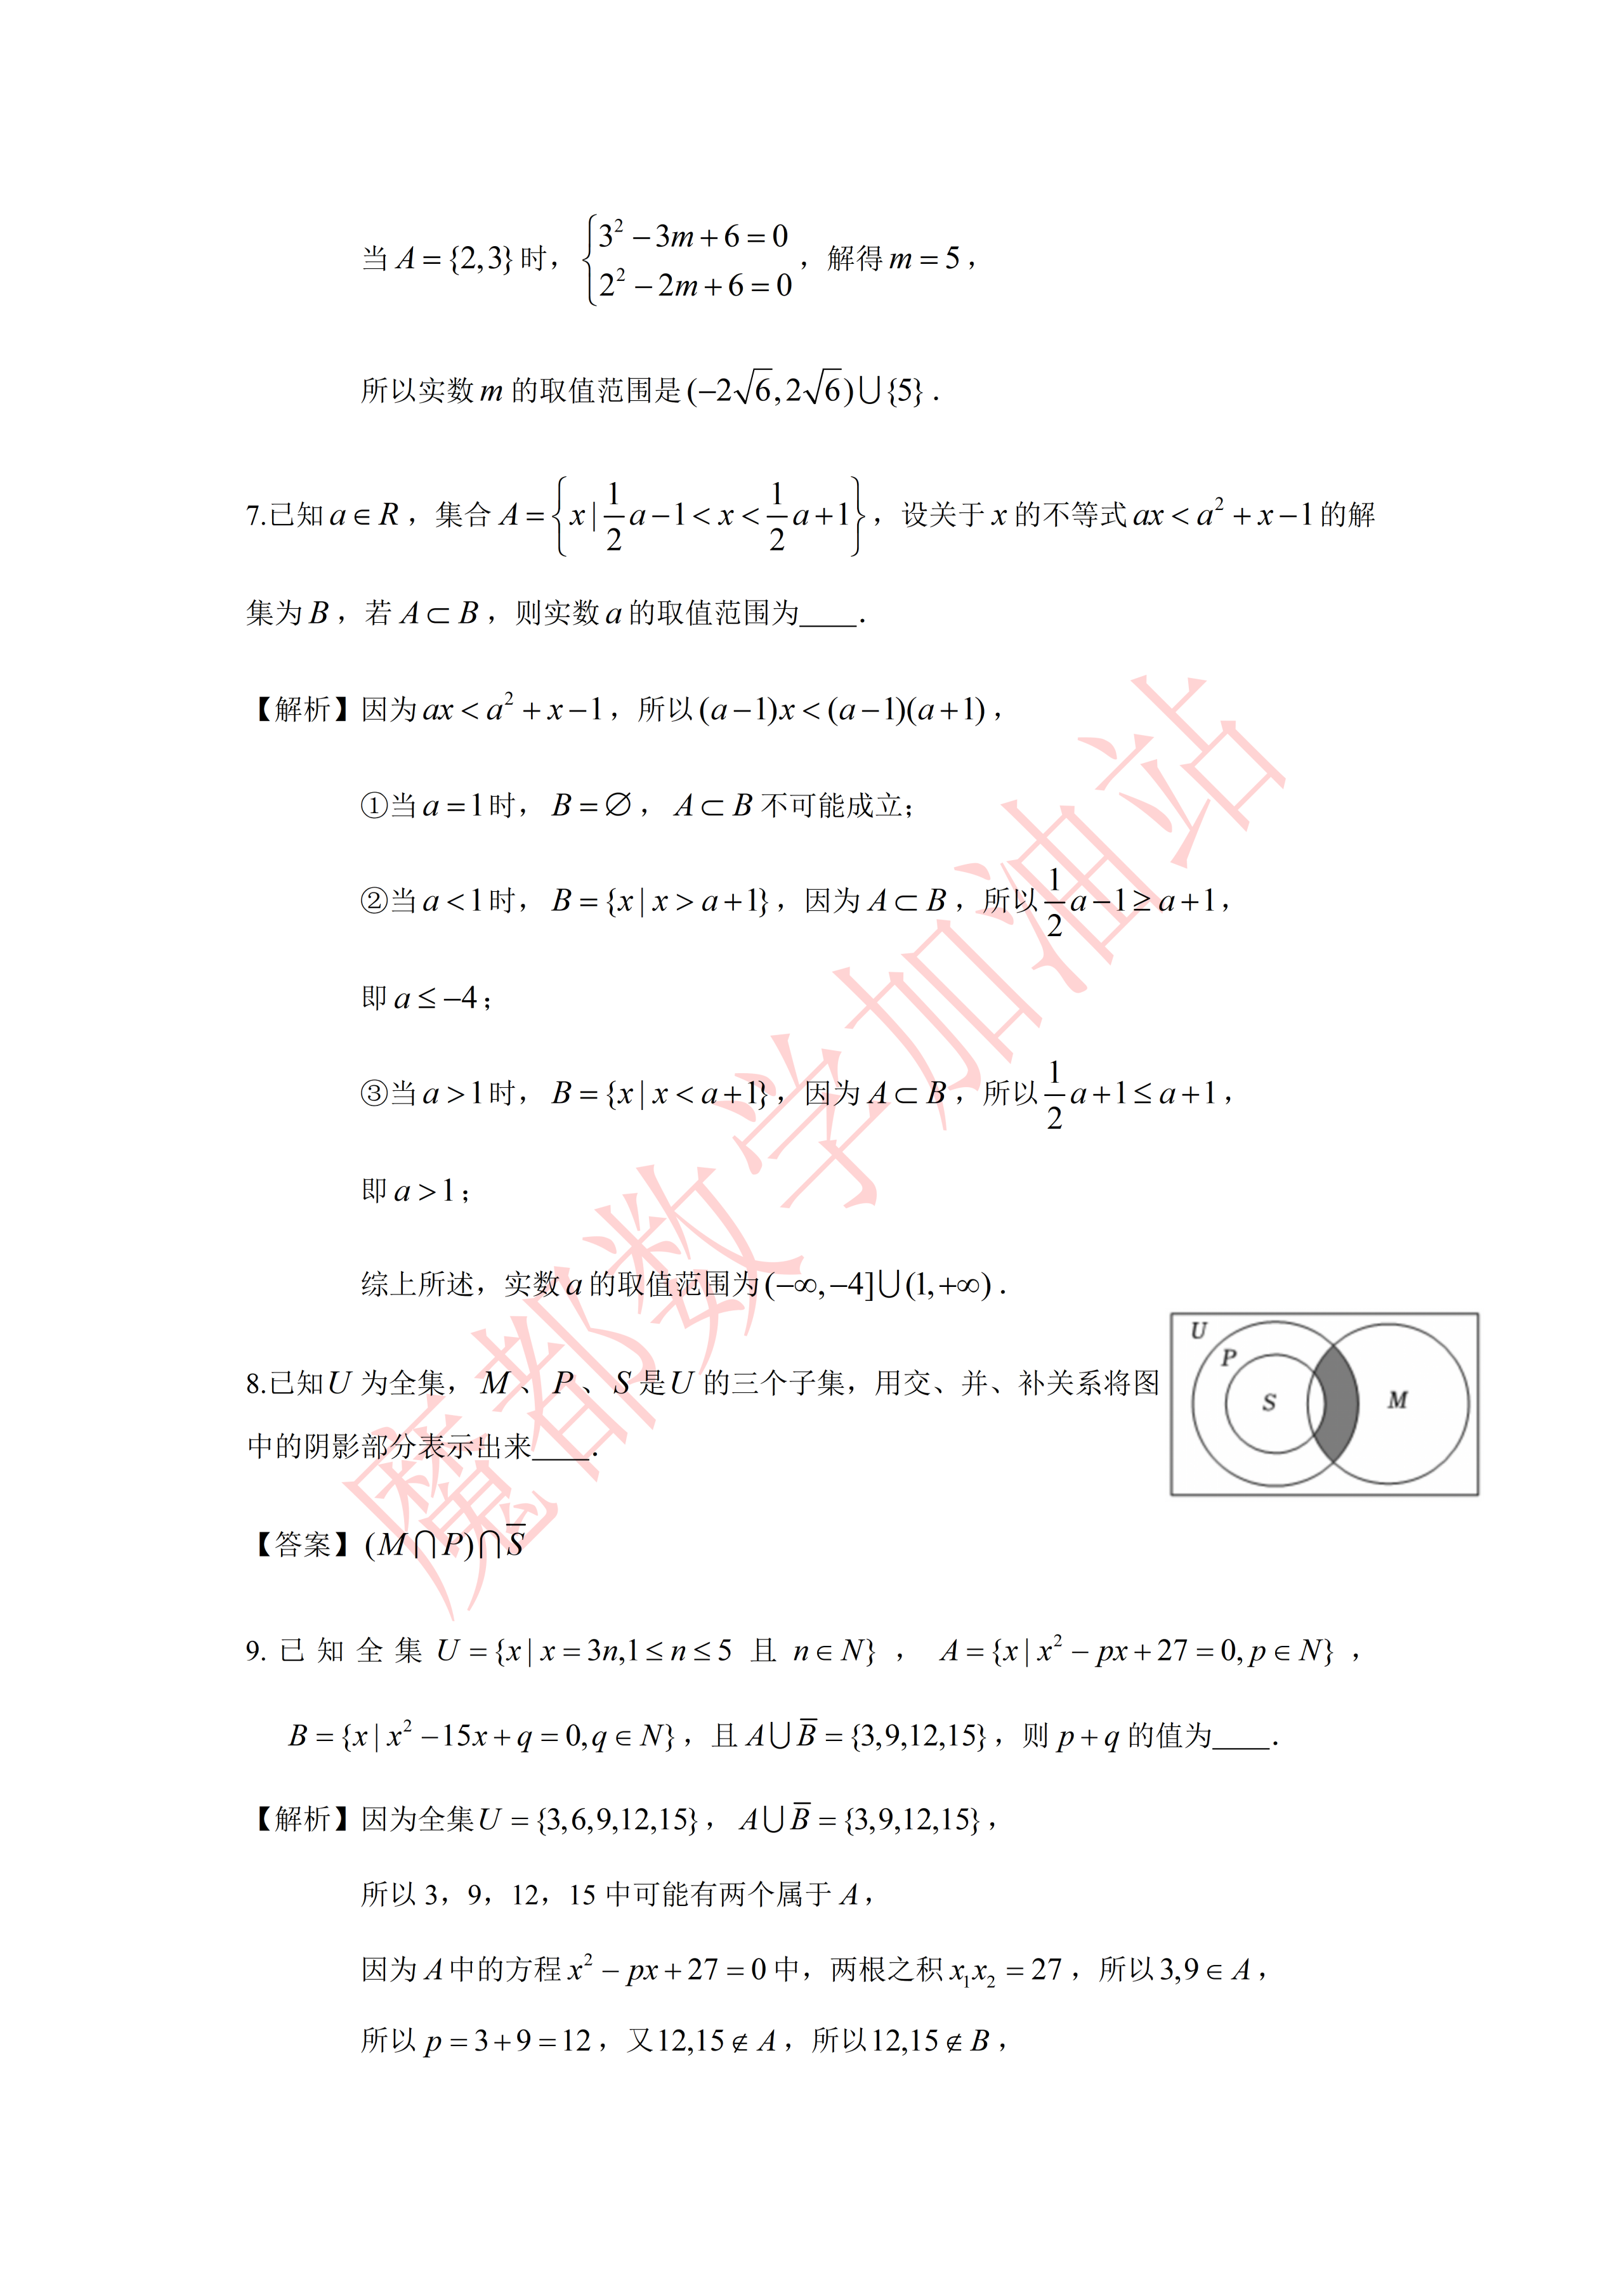
\includegraphics[width=.38\linewidth,trim=1835bp 1255bp 220bp 1565bp,clip]{../原图/高一49_华师大二附中_国庆作业1/02.png}
\end{center}

\ifanswer
\ans{$(M\cap P)\cap\overline S$}
\fi

\item 已知全集 $U=\{x\mid x=3n,1\leqslant n\leqslant5\text{ 且 }n\in\N\}$，$A=\{x\mid x^2-px+27=0,p\in\N\}$，$B=\{x\mid x^2-15x+q=0,q\in\N\}$，且 $A\cup\overline B=\{3,9,12,15\}$，则 $p+q$ 的值为\blankline[4.4em].

\ifanswer
\solbegin
\step{因为全集 $U=\{3,6,9,12,15\}$，$A\cup\overline B=\{3,9,12,15\}$，}
\step{所以 $3$、$9$、$12$、$15$ 中可能有两个属于 $A$，}
\step{因为 $A$ 中的方程 $x^2-px+27=0$ 中，两根之积 $x_1x_2=27$，所以 $3,9\in A$，}
\step{所以 $p=3+9=12$，又 $12,15\notin A$，所以 $12,15\notin B$，}
\step{因为 $B$ 中的方程 $x^2-15x+q=0$ 中，两根之和 $x_3+x_4=15$，所以 $6,9\in B$，}
\step{则 $q=6\times9=54$，所以 $p+q=66$.}
\solend
\fi

\item 已知集合 $A=\{x\mid x^2+(2a-3)x-3a=0,a\in\R,x\in\R\}$，集合 $B=\{x\mid x^2+(a-3)x+a^2-3a=0,a\in\R,x\in\R\}$，若 $A\neq B$，$A\cap B\neq\varnothing$，则 $A\cup B=$\blankline[4.4em].

\ifanswer
\solbegin
\step{设两个集合中的方程的公共解是 $b$，}
\step{由 $b^2+(2a-3)b-3a=b^2+(a-3)b+a^2-3a$，得 $ab=a^2$，}
\step{则 $a=0$ 或 $b=a$，}
\step{当 $a=0$ 时，不合题意，}
\step{当 $b=a$ 时，即两个方程的公共解为 $b=a$，}
\step{将 $b=a$ 代入方程，得 $a^2=2a$，$a=2$，}
\step{所以 $A=\{2,-3\}$，$B=\{-1,2\}$，所以 $A\cup B=\{-1,2,-3\}$.}
\solend
\fi

\item 已知一个有四个数字元素的集合 $S$，$S$ 的所有子集的元素和（空集的元素和认为是 $0$）的总和为 $16192$，则 $S$ 的元素之和等于\blankline[4.4em].

\ifanswer
\solbegin
\step{设 $S=\{a_1,a_2,a_3,a_4\}$，$S$ 的每个元素在所有子集中均出现 $2^3$ 次，}
\step{故 $(a_1+a_2+a_3+a_4)\cdot2^3=16192$，所以 $a_1+a_2+a_3+a_4=2024$，}
\step{故 $S$ 的元素之和等于 $2024$.}
\solend
\fi

\item 设 $P$ 为非空实数集满足：对任意给定的 $x,y\in P$（$x$、$y$ 可以相同），都有 $x+y\in P,x-y\in P,xy\in P$，则称 $P$ 为封闭集．关于封闭集有下列结论：

①集合 $P=\{-2,-1,0,1,2\}$ 为封闭集；

②集合 $P=\{x\mid x=2n,n\in\Z\}$ 为封闭集；

③若集合 $P_1$、$P_2$ 为封闭集，则 $P_1\cup P_2$ 为封闭集；

④若集合 $P$ 为封闭集，则一定有 $0\in P$；

⑤若集合 $P_1$、$P_2$ 为封闭集，则 $P_1\cap P_2$ 为封闭集.

其中正确结论的序号是\blankline[4.4em].

\ifanswer
\solbegin
\step{对于集合 $P=\{-2,-1,0,1,2\}$，取 $x=2$，$y=-2$，则 $x-y=2-(-2)=4\notin P$，}
\step{不满足封闭集的定义，所以①错误.}
\step{对于集合 $P=\{x\mid x=2n,n\in\Z\}$，设 $x=2n_1$，$y=2n_2$，$n_1,n_2\in\Z$.}
\step{$x+y=2n_1+2n_2=2(n_1+n_2)$，因为 $n_1+n_2\in\Z$，所以 $x+y\in P$.}
\step{$x-y=2n_1-2n_2=2(n_1-n_2)$，因为 $n_1-n_2\in\Z$，所以 $x-y\in P$.}
\step{$xy=2n_1\times2n_2=4n_1n_2=2(2n_1n_2)$，因为 $2n_1n_2\in\Z$，所以 $xy\in P$.}
\step{满足封闭集的定义，所以②正确.}
\step{令 $P_1=\{x\mid x=2n,n\in\Z\}$，$P_2=\{x\mid x=3n,n\in\Z\}$，都是封闭集.}
\step{$P_1\cup P_2$ 中，取 $x=2(x\in P_1)$，$y=3(y\in P_2)$，$x+y=5\notin P_1\cup P_2$，}
\step{不满足封闭集的定义，所以③错误.}
\step{因为对任意 $x\in P$，有 $x-x=0\in P$，}
\step{所以若集合 $P$ 为封闭集，则一定有 $0\in P$，所以④正确.}
\step{因为 $P_1$、$P_2$ 为封闭集，设 $x,y\in P_1\cap P_2$，则 $x,y\in P_1$ 且 $x,y\in P_2$.}
\step{因为 $P_1$ 是封闭集，所以 $x+y\in P_1,x-y\in P_1,xy\in P_1$.}
\step{因为 $P_2$ 是封闭集，所以 $x+y\in P_2,x-y\in P_2,xy\in P_2$.}
\step{所以 $x+y\in P_1\cap P_2,x-y\in P_1\cap P_2,xy\in P_1\cap P_2$，满足封闭集的定义，}
\step{所以⑤正确.}
\step{故正确的是②④⑤.}
\solend
\fi

\end{enumerate}

\bigsec{二、选择题}

\begin{enumerate}
\setcounter{enumi}{12}

\item 已知集合 $A=\{1,3,\sqrt m\}$，$B=\{1,m\}$，$B\subseteq A$，则 $m=$\mbox{（\quad）}

\keepwithprev
A. $0$ 或 $\sqrt3$\qquad B. $0$ 或 $3$

C. $1$ 或 $\sqrt3$\qquad D. $1$ 或 $3$

\ifanswer
\solbegin
\step{因为集合 $A=\{1,3,\sqrt m\}$，$B=\{1,m\}$，$B\subseteq A$，所以 $m=3$ 或 $m=\sqrt m$，}
\step{若 $m=3$，$A=\{1,3,\sqrt3\}$，$B=\{1,3\}$，满足 $B\subseteq A$，}
\step{若 $m=\sqrt m$，解得 $m=1$ 或 $m=0$，}
\step{①若 $m=0$，则 $A=\{1,3,0\}$，$B=\{1,0\}$，满足 $B\subseteq A$.}
\step{②若 $m=1$，则 $A$、$B$ 不满足集合中元素的互异性，舍去.}
\step{综上，$m=0$ 或 $m=3$．故选 $B$.}
\solend
\fi

\needvspace{10\baselineskip}

\item 设集合 $A$、$B$、$C$、$D$ 是全集 $X$ 的子集，$A\cap B\neq\varnothing$，$A\cap C\neq\varnothing$，则下列选项中正确的是\mbox{（\quad）}

\keepwithprev
A. 如果 $D\subset B$ 或 $D\subset C$，则 $D\cap A\neq\varnothing$

B. 如果 $D\subset A$，则 $\overline D\cap B\neq\varnothing$，$\overline D\cap C\neq\varnothing$

C. 如果 $A\subset D$，则 $\overline D\cap B=\varnothing$，$\overline D\cap C=\varnothing$

D. 上述各项都不正确

\ifanswer
\solbegin
\step{用韦恩图表示每个选项：}
\begin{center}
% 原图第 5 页解析配图（三联韦恩图）直接裁取（原卷排于选项 C、D 右侧）。
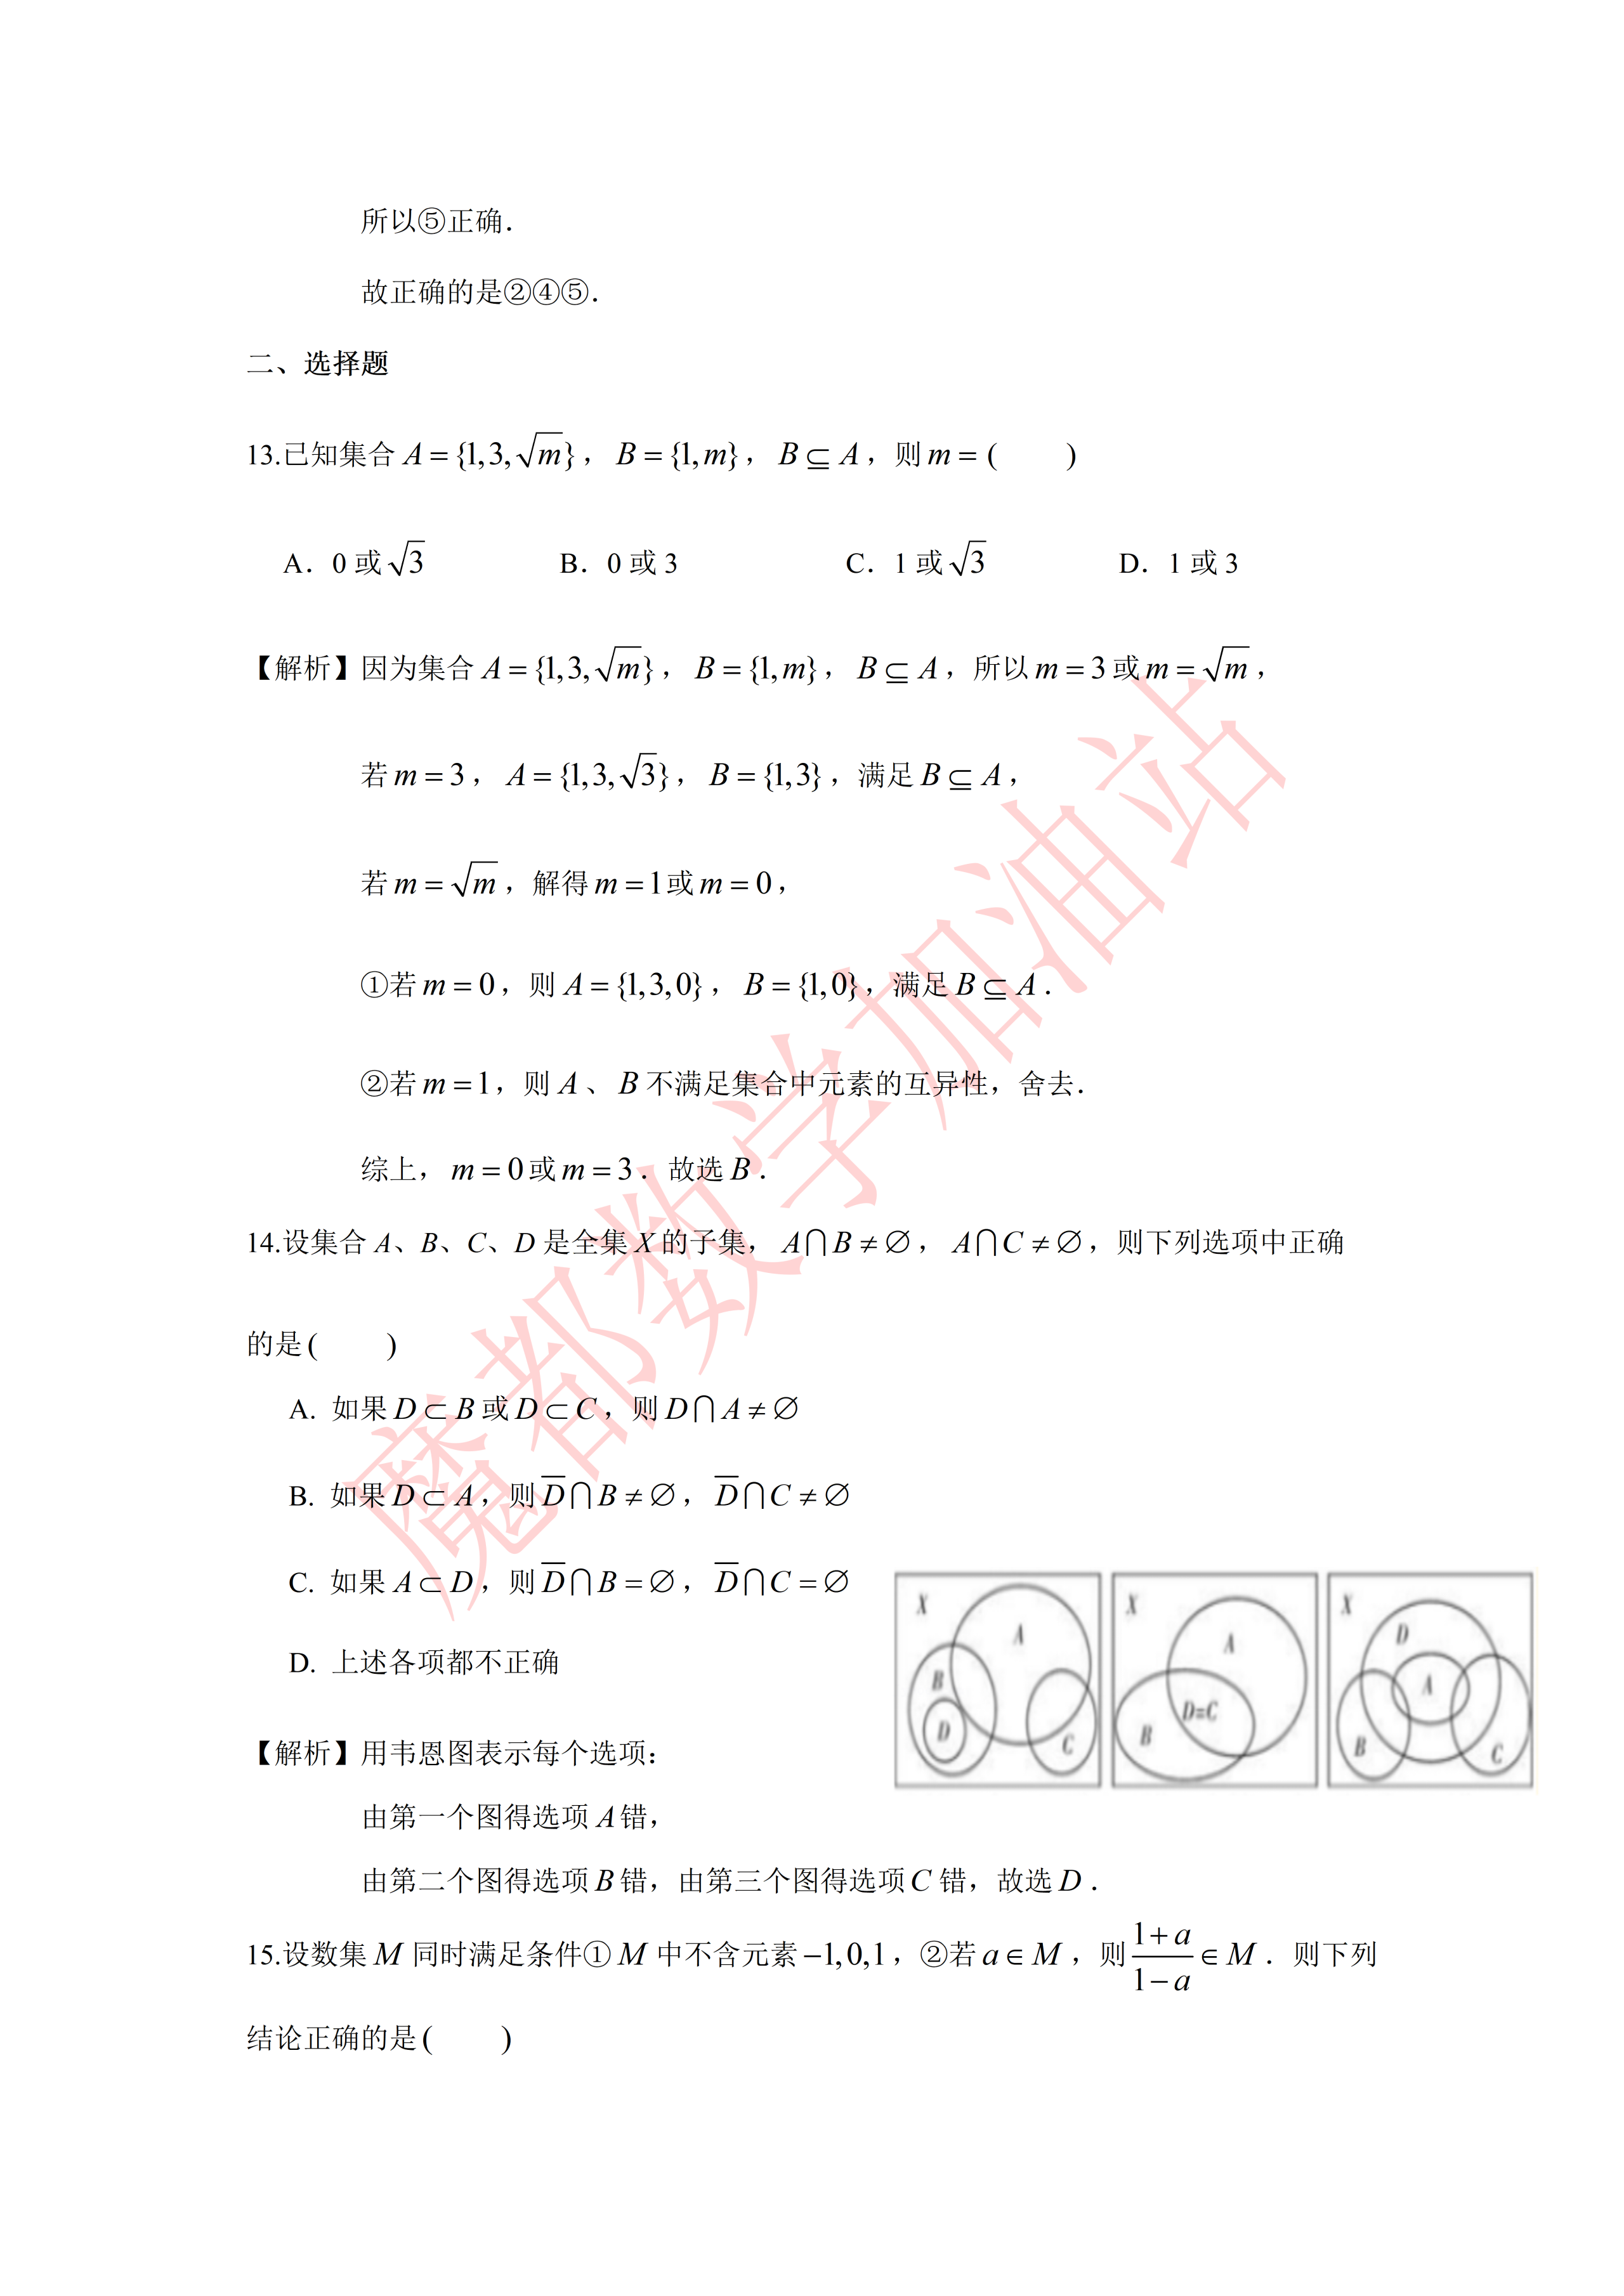
\includegraphics[width=.75\linewidth,trim=1400bp 790bp 135bp 1155bp,clip]{../原图/高一49_华师大二附中_国庆作业1/05.png}
\end{center}
\step{由第一个图得选项 $A$ 错，}
\step{由第二个图得选项 $B$ 错，由第三个图得选项 $C$ 错，故选 $D$.}
\solend
\fi

\item 设数集 $M$ 同时满足条件①$M$ 中不含元素 $-1$、$0$、$1$，②若 $a\in M$，则 $\dfrac{1+a}{1-a}\in M$．则下列结论正确的是\mbox{（\quad）}

\keepwithprev
A. 集合 $M$ 中至多有 $2$ 个元素\qquad B. 集合 $M$ 中至多有 $3$ 个元素

C. 集合 $M$ 中有且仅有 $4$ 个元素\qquad D. 集合 $M$ 中有无穷多个元素

\ifanswer
\solbegin
\step{若集合只含有一个元素，则 $\dfrac{1+a}{1-a}=a$，即 $1+a=a-a^2$，即 $-a^2=1$，不成立.}
\step{当 $a=3$ 时，$\dfrac{1+3}{1-3}=-2\in M$，所以 $\dfrac{1-2}{1+2}=-\dfrac13\in M$，所以 $\dfrac{1-\frac13}{1+\frac13}=\dfrac12\in M$，}
\step{所以 $\dfrac{1+\frac12}{1-\frac12}=3$，开始重复了，所以 $M=\left\{3,-2,-\dfrac13,\dfrac12\right\}$；}
\step{当 $a=2$ 时，$\dfrac{1+2}{1-2}=-3\in M$，所以 $\dfrac{1-3}{1+3}=-\dfrac12\in M$，所以 $\dfrac{1-\frac12}{1+\frac12}=\dfrac13\in M$，}
\step{所以 $\dfrac{1+\frac13}{1-\frac13}=2$，开始重复了，所以 $M=\left\{2,-3,-\dfrac12,-\dfrac13\right\}$，}
\step{此时也只要四个元素；}
\step{当 $a=\dfrac34\in M$，则 $7\in M$，若 $7\in M$，则 $-\dfrac43\in M$，}
\step{若 $-\dfrac43\in M$，则 $-\dfrac17\in M$，若 $-\dfrac17\in M$，有 $\dfrac34\in M$，}
\step{由归纳推理得，集合 $M$ 中有且仅有 $4$ 个元素．故选 $C$.}
\solend
\fi

\item 已知集合 $M=\{x\mid x\in\N,0<x\leqslant15\}$，$A_1$、$A_2$、$A_3$ 满足：①$A_1\cup A_2\cup A_3=M$；②每个集合都恰有 $5$ 个元素．集合 $A_i$（$i=1,2,3$）中最大元素与最小元素之和称为 $A_i$ 的特征数，记为 $X_i$（$i=1,2,3$），则 $X_1+X_2+X_3$ 的值不可能为\mbox{（\quad）}

\keepwithprev
A. $37$\qquad B. $39$\qquad C. $48$\qquad D. $57$

\ifanswer
\solbegin
\step{因为集合 $M=\{x\mid x\in\N,0<x\leqslant15\}=\{1,2,3,\cdots,15\}$，}
\step{又因为集合 $A_1$、$A_2$、$A_3$ 中，每个集合恰有 $5$ 个元素，}
\step{且 $A_1\cup A_2\cup A_3=M$ 有 $15$ 个元素，所以集合 $A_1$、$A_2$、$A_3$ 中没有重复元素，}
\step{因为 $1$ 是集合 $M$ 中数值最小的元素，$15$ 是集合 $M$ 中数值最大的元素，}
\step{所以在 $A_i$ 的特征数构成中，必有 $1$ 和 $15$，不妨设 $1\in A_1$，$15\in A_1$，}
\step{要使 $X_1+X_2+X_3$ 最大，则应该在集合 $A_1$ 中首先放置数值较小的元素，}
\step{即 $A_1=\{1,2,3,4,15\}$，所以 $5$ 与 $14$ 是剩下元素中数值最小或最大的元素，}
\step{同理，不妨设 $5\in A_2$，$14\in A_2$，接着在 $A_2$ 中再次放置数值较小的元素，}
\step{即 $A_2=\{5,6,7,8,14\}$，则 $A_3=\{9,10,11,12,13\}$，}
\step{此时 $X_1+X_2+X_3$ 有最大值为 $1+15+5+14+9+13=57$，}
\step{即 $X_1+X_2+X_3\leqslant57$；}
\step{要使 $X_1+X_2+X_3$ 最小，则在集合 $A_1$ 中首先放置数值较大的元素，}
\step{即 $A_1=\{1,12,13,14,15\}$，所以 $2$ 与 $11$ 是剩下元素中数值最小或最大的元素，}
\step{同理，不妨设 $2\in A_2$，$11\in A_2$，接着在 $A_2$ 中再次放置数值较大的元素，}
\step{即 $A_2=\{2,8,9,10,11\}$，则 $A_3=\{3,4,5,6,7\}$，}
\step{此时 $X_1+X_2+X_3$ 有最小值为 $1+15+2+11+3+7=39$，}
\step{即 $X_1+X_2+X_3\geqslant39$，}
\step{综上，$39\leqslant X_1+X_2+X_3\leqslant57$，故选 $A$.}
\solend
\fi

\end{enumerate}

\bigsec{三、解答题}

\begin{enumerate}
\setcounter{enumi}{16}

\item 已知全集为 $\R$，集合 $A=\{x\mid y=\sqrt{(2+x)(4-x)}\}$，$B=\{x\mid-1<x<m+1\}$.

\begin{enumerate}[label=(\arabic*)]
\item 若 $m=4$，求 $A\cup B$、$\overline A\cap B$；
\item 若 $B\subseteq A$，求实数 $m$ 的取值范围.
\end{enumerate}

\ifanswer
\solbegin
\stepm{(1)}{集合 $A=\{x\mid y=\sqrt{(2+x)(4-x)}\}=\{x\mid-2\leqslant x\leqslant4\}$，}
\step{当 $m=4$ 时，$B=\{x\mid-1<x<5\}$.}
\step{所以 $A\cup B=[-2,5)$，$\overline A=\{x\mid x<-2\text{ 或 }x>4\}$，$\overline A\cap B=(4,5)$.}
\stepm{(2)}{因为 $B\subseteq A$，}
% 原卷如此，照录未改（第 17 题(2)解析两处"当 C=∅／当 C≠∅"应为 B，本卷并无集合 C）
\step{当 $C=\varnothing$ 时，$m\leqslant-2$，$B\subseteq A$ 成立；}
\step{当 $C\neq\varnothing$ 时，$m>-2$，$-1<m+1\leqslant4$，解得 $-2<m\leqslant3$，}
\step{综上，$m\leqslant3$，所以实数 $m$ 的取值范围是 $(-\infty,3]$.}
\solend
\fi

\ansspace[6]

\item 用反证法证明：若 $a$、$b$、$c\in\R$，且 $x=a^2-2b+1$，$y=b^2-2c+1$，$z=c^2-2a+1$，则 $x$、$y$、$z$ 中至少有一个不小于 $0$.

\ifanswer
\solbegin
\step{假设 $x$、$y$、$z$ 均小于 $0$，即 $x=a^2-2b+1<0$①，$y=b^2-2c+1<0$②，}
\step{$z=c^2-2a+1<0$③，①$+$②$+$③得 $x+y+z=(a-1)^2+(b-1)^2+(c-1)^2<0$，}
\step{这与 $(a-1)^2+(b-1)^2+(c-1)^2\geqslant0$ 矛盾，则假设不成立，}
\step{所以 $x$、$y$、$z$ 中至少有一个不小于 $0$，得证.}
\solend
\fi

\ansspace[5]

\item 已知全集为 $\R$，实数 $a$、$b$ 满足 $a\neq b$，集合 $M=\{x\mid x^2-3x-4\leqslant0\}$，集合 $A=\{x\mid(x+a)(x+b)>0\}$，集合 $B=\{x\mid x^2+(a-2)x-2a>0\}$.

\begin{enumerate}[label=(\arabic*)]
\item 若 $\overline A=M$，求 $a$、$b$ 的值；
\item 若 $a>b>-1$，求 $A\cap B$；
\item 若 $a^2+a\in\overline B$，求 $a$ 的取值范围.
\end{enumerate}

\ifanswer
\solbegin
\stepm{(1)}{$M=\{x\mid x^2-3x-4\leqslant0\}=\{x\mid-1\leqslant x\leqslant4\}$，$A=\{x\mid(x+a)(x+b)\leqslant0\}$，}
\step{因为 $\overline A=M$，所以 $a=1$，$b=-4$ 或 $a=-4$，$b=1$.}
\stepm{(2)}{因为 $a>b>-1$，所以 $-a<-b<1$，所以 $A=\{x\mid x<-a\text{ 或 }x>-b\}$，}
\step{因为 $B=\{x\mid x^2+(a-2)x-2a>0\}=\{x\mid x<-a\text{ 或 }x>2\}$，}
\step{所以 $A\cap B=\{x\mid x<-a\text{ 或 }x>2\}$，}
\stepm{(3)}{$\overline B=\{x\mid(x-2)(x+a)\leqslant0\}$，}
% 原卷如此，照录未改（第 19 题(3)此处"a(a-1)((a-2)^2≤0"括号不配对；且由左式展开应为
% a(a-1)(a+2)^2≤0，与下句"解得 a=2 …[0,1]∪{2}"按 (a-2)^2 方自洽，见文件头清单第 2 条）
\step{由 $a^2+a\in\overline B$，得 $(a^2+a-2)(a^2+2a)\leqslant0\Leftrightarrow a(a-1)((a-2)^2\leqslant0$，}
\step{解得 $a=2$ 或 $0\leqslant a\leqslant1$，故 $a$ 的取值范围是 $[0,1]\cup\{2\}$.}
\solend
\fi

\ansspace[7]

\item 设数集 $A$ 由实数构成，若 $x\in A$（$x\neq1$ 且 $x\neq0$），则 $\dfrac{1}{1-x}\in A$.

\begin{enumerate}[label=(\arabic*)]
\item 若 $2\in A$，则 $A$ 中至少还有几个元素；
\item 集合 $A$ 是否为双元素集合？请说明理由；
\item 若 $A$ 中元素个数不超过 $8$ 个，所有元素的和为 $\dfrac{14}{3}$，且 $A$ 中有一个元素的平方等于所有元素的积，求集合 $A$.
\end{enumerate}

\ifanswer
\solbegin
\stepm{(1)}{若 $x\in A$，则 $\dfrac{1}{1-x}\in A$，又 $2\in A$，所以 $\dfrac{1}{1-2}=-1\in A$，}
\step{所以 $\dfrac{1}{1-(-1)}=\dfrac12\in A$，所以 $\dfrac{1}{1-\frac12}=2\in A$，}
% 原卷如此，照录未改（第 20 题(1)解析末句"2 个几个元素"衍一"几个"）
\step{所以 $A$ 中至少还有 $2$ 个几个元素；}
\stepm{(2)}{若 $x\in A$（$x\neq1$ 且 $x\neq0$），则 $\dfrac{1}{1-x}\in A$，}
\step{则 $\dfrac{1}{1-\frac{1}{1-x}}=\dfrac{1-x}{-x}\in A$，则 $\dfrac{1}{1-\frac{1-x}{-x}}=x\in A$}
\step{若 $A$ 为双元素集，则 $x=\dfrac{1}{1-x}$ 或 $x=\dfrac{1-x}{-x}$ 或 $\dfrac{1}{1-x}=\dfrac{1-x}{-x}$，均无解，}
\step{所以 $A$ 不可能为双元素集；}
\stepm{(3)}{由 $x\in A$，$\dfrac{1}{1-x}\in A$，得 $\dfrac{1}{1-\frac{1}{1-x}}=\dfrac{x-1}{x}\in A$，得 $\dfrac{1}{1-\frac{x-1}{x}}=x\in A$，}
\step{所以 $\left\{x,\dfrac{1}{1-x},\dfrac{x-1}{x}\right\}\subseteq A$，而 $x\cdot\dfrac{1}{1-x}\cdot\dfrac{x-1}{x}=-1$，}
\step{$A$ 中元素个数为 $3$ 的倍数，则 $A$ 中元素只有 $6$ 个，}
\step{因为 $A$ 中有一个元素的平方等于所有元素的积，}
\step{不妨设 $x^2=1$，解得 $x=-1$ 或 $x=1$（舍），则 $-1$、$\dfrac12$、$2\in A$，}
\step{所以 $-1+\dfrac12+2+m+\dfrac{1}{1-m}+\dfrac{m-1}{m}=\dfrac{14}{3}$，解得 $m=-\dfrac12$ 或 $m=3$ 或 $m=\dfrac23$，}
\step{所以 $A=\left\{\dfrac12,2,-1,-\dfrac12,3,\dfrac23\right\}$.}
\solend
\fi

\ansspace[9]

% 原卷如此，照录未改（第 21 题题干"21.求已知集合"之"求"字疑衍；"任意两个元素 a_i a_j"
% 疑脱逗号；"|a_i-a_j|≥1/30 则称"之前疑脱标点，见文件头清单第 4 条）
\item 求已知集合 $M=\left\{\dfrac{1}{k}\middle|1\leqslant k\leqslant100\text{ 且 }k\in\N^{*}\right\}$，$A=\{a_1,a_2,\cdots,a_n\}$，其中 $n\in\N^{*}$，且 $n\geqslant2$．若 $A\subseteq\N$，且对集合 $A$ 中的任意两个元素 $a_ia_j$，$i\neq j$ 都有 $|a_i-a_j|\geqslant\dfrac{1}{30}$ 则称集合 $A$ 有性质 $P$.

\begin{enumerate}[label=(\arabic*)]
\item 判断集合 $\left\{\dfrac13,\dfrac14,\dfrac15,\dfrac16,\dfrac17\right\}$ 是否具有性质 $P$；
\item 若集合 $A=\{a_1,a_2,\cdots,a_n\}$ 具有性质 $P$.

①求证：$a_i-a_j$ 的最大值大于等于 $\dfrac{n-1}{30}$；

②求 $A$ 的元素个数 $n$ 的最大值.
\end{enumerate}

\ifanswer
\solbegin
\stepm{(1)}{集合为 $\left\{\dfrac13,\dfrac14,\dfrac15,\dfrac16,\dfrac17\right\}$，又 $\dfrac16-\dfrac17=\dfrac{1}{42}<\dfrac{1}{30}$，所以该集合不具有性质 $P$；}
\stepm{(2)}{①因为集合 $A=\{a_1,a_2,\cdots,a_n\}$ 具有性质 $P$，}
\step{不妨设 $a_1<a_2<a_3<\cdots<a_n$，则 $a_i-a_j\geqslant\dfrac{1}{30}$（$i>j$），}
\step{所以 $a_n-a_1=(a_n-a_{n-1})+(a_{n-1}-a_{n-2})+\cdots+(a_2-a_1)\geqslant\dfrac{n-1}{30}$，}
\step{故 $a_i-a_j$ 的最大值大于等于 $\dfrac{n-1}{30}$；}
% 原卷如此，照录未改（第 21 题(2)②首行"a_2-a_1≥(n-1)/30"：由①同款推理只能得
% a_2-a_1≥1/30，见文件头清单第 5 条）
\step{②$A=\{a_1,a_2,\cdots,a_n\}$，不妨设 $a_1<a_2<a_3<\cdots<a_n$，}
\step{要使 $A$ 的元素个数 $n$ 最大，}
\step{则 $A$ 中的元素满足 $a_n=\dfrac{1}{k}$，$a_{n-1}=\dfrac{1}{k+1}$，$\cdots$，$a_1=\dfrac{1}{k+n-1}$（$k\in\N^{*}$），}
\step{又由①得 $a_2-a_1=\dfrac{1}{k+n-2}-\dfrac{1}{k+n-1}\geqslant\dfrac{n-1}{30}$，}
\step{所以 $(k+n-2)(k+n-1)\leqslant30$，又 $a_n-a_{n-1}=\dfrac{1}{k}-\dfrac{1}{k+1}\geqslant\dfrac{1}{30}$，}
\step{所以 $k(k+1)\leqslant30$，所以 $1\leqslant k\leqslant5$（$k\in\N^{*}$），}
\step{当 $k=5$ 时，由 $(k+n-2)(k+n-1)\leqslant30$，解得 $n\leqslant2$，$n\in\N^{*}$；}
\step{当 $k=4$ 时，由 $(k+n-2)(k+n-1)\leqslant30$，解得 $n\leqslant3$，$n\in\N^{*}$；}
\step{当 $k=3$ 时，由 $(k+n-2)(k+n-1)\leqslant30$，解得 $n\leqslant4$，$n\in\N^{*}$；}
\step{当 $k=2$ 时，由 $(k+n-2)(k+n-1)\leqslant30$，解得 $n\leqslant5$，$n\in\N^{*}$；}
\step{当 $k=1$ 时，由 $(k+n-2)(k+n-1)\leqslant30$，解得 $n\leqslant6$，$n\in\N^{*}$.}
\step{故 $A$ 的元素个数 $n$ 的最大值为 $6$，此时集合 $A=\left\{1,\dfrac12,\dfrac13,\cdots,\dfrac16\right\}$.}
\solend
\fi

\ansspace*[10]

\end{enumerate}

\end{document}
"
%
% 原始材料：微信公众号"魔都数学加油站"文章，作者破晓，连载"27学年高一49"；
% 原文标题"27学年高一49——2026-2027年上海市华师大二附中高一上国庆作业1集合与逻辑、
% 等式与不等式的性质"；页面用 JS 渲染，未见明确发布日期（页内时间戳 ≈ 2026-10-05 21:37）；
% 原文链接：https://mp.weixin.qq.com/s/XxZTOBVQslK5cZm2_BbhOg。
% 正文为 11 张 PNG 页：第 01、03、04、06、07、08、09 页 4762×6735，
% 第 02、05、10、11 页 2560×3620，均按页序读取；粉色斜排"魔都数学加油站"为卷面水印，
% 与公众号页脚一并未录入。全卷 11 页均为试卷页，无二维码/宣传页。
%
% 题号与分节：原文自第 3 题起编，填空题 3—12、选择题 13—16、解答题 17—21，共 19 题。
% 讲评版：原卷每题下直接印【答案】或【解析】——只印【答案】的 3 题（第 3、5、8 题），
% 其余 16 题均只印【解析】；解析行数已逐题按印刷行照录（一条 \step＝原卷一个印刷行）。
%
% 卷首标题：照卷面印作"2026-2027 年华师大二附中高一上国庆作业 1"（公众号标题中的"上海市"
% 卷面没有，本稿照卷面），年份区间按全稿惯例排 en dash；副标题照卷面自印的
% "集合与逻辑单元综合检测"（原卷页首标题行下方即印此行，故不另按模块口径拟名）。
% 副标题依据：全卷 19 题均为集合与常用逻辑用语内容——集合类 15 题（6—17、19—21 中除
% 反证法题外），逻辑/命题类 3 题（第 3 题否定形式、第 4 题充要条件、第 5 题反证法假设），
% 反证法证明 1 题（第 18 题）；全卷无不等式求解题，公众号标题中"等式与不等式的性质"
% 与卷面实际内容不符。
%
% 与原卷的排版差异：
%   ① 原文从第 3 题起，填空题为 3—12、选择题为 13—16、解答题为 17—21，本稿保留原题号；
%   ② 原卷每题下直接印【答案】/【解析】，本稿按全稿惯例置于答案版；只印【解析】的题
%      不另提 \ans{}（照 高一36 口径），只印【答案】的题仅给 \ans{}；
%   ③ 原卷第 8 题韦恩图排在题干右侧、第 14 题三联韦恩图排在选项（C、D）右侧，
%      本稿分别移至题干下方、解析首步之后居中排，均直接裁取原图页（02.png、05.png）；
%   ④ 数集记号原卷排作斜体/加粗 R、N、Z，本稿统一为 \R、\N、\Z、\N^*；
%      填空横线按全稿惯例排为 \blankline[4.4em]。
%
% 原卷笔误/存疑清单（均照录未改，正文中该处有 % 注）：
%   1. 第 17 题(2)解析两处"当 C=∅／当 C≠∅"应为 B（本卷并无集合 C）；
%   2. 第 19 题(3)解析"a(a-1)((a-2)^2≤0"括号不配对（多一枚左括号）；且由
%      (a^2+a-2)(a^2+2a)≤0 展开应为 a(a-1)(a+2)^2≤0，与原卷结论"解得 a=2 …
%      [0,1]∪{2}"恰按 (a-2)^2 自洽——因式分解与原式不符，结论按 (a-2)^2 自洽，均照录；
%   3. 第 20 题(1)解析末句"至少还有 2 个几个元素"衍一"几个"；
%   4. 第 21 题题干"21.求已知集合"之"求"字疑衍；"任意两个元素 a_i a_j"疑脱逗号；
%      "≥1/30 则称"之前疑脱标点；
%   5. 第 21 题(2)②解析"a_2-a_1≥(n-1)/30"：由①同款推理只能得 a_2-a_1≥1/30，
%      原卷如此，照录未改（后续 (k+n-2)(k+n-1)≤30 即按该行推得）。
%
\documentclass[a4paper,11pt]{article}
\usepackage{common}

\begin{document}

\examtitlest[3]{2026--2027 年华师大二附中高一上国庆作业 1}{集合与逻辑单元综合检测}

\bigsec{一、填空题}

\begin{enumerate}
\setcounter{enumi}{2}

\item “若 $x^2-x-2\leqslant0$，则 $-1\leqslant x\leqslant2$”的否定形式为\blankline[4.4em].

\ifanswer
\ans{若 $x^2-x-2>0$，则 $x<-1$ 或 $x>2$}
\fi

\item 已知 $p:|x-3|<5$，$q:1-a<x<2a-3$，且 $p$ 是 $q$ 的充分非必要条件，则实数 $a$ 的取值范围是\blankline[4.4em].

\ifanswer
\solbegin
\step{由 $|x-3|<5$ 得 $-2<x<8$，}
\step{又 $p$ 是 $q$ 的充分不必要条件，所以 $(-2,8)\subset(1-a,2a-3)$，}
\step{即 $\begin{cases}-2\geqslant1-a\\ 8\leqslant2a-3\\ (2a-3)-(1-a)\neq8-(-2)\end{cases}$，解得 $a\geqslant\dfrac{11}{2}$，实数 $a$ 的取值范围是 $\left[\dfrac{11}{2},+\infty\right)$.}
\solend
\fi

\item 用反证法证明命题“设 $a$、$b\in\R$，则方程 $a_1x^2+b_1x+c_1=0$ 与 $a_2x^2+b_2x+c_2=0$ 至少有一个实根”时要做的假设是\blankline[4.4em].

\ifanswer
\ans{假设 $a$、$b\in\R$，方程 $a_1x^2+b_1x+c_1=0$ 与 $a_2x^2+b_2x+c_2=0$ 都没有实根}
\fi

\item 设集合 $A=\{x\mid x^2-mx+6=0,x\in\R\}$，且 $A\cap\{2,3\}=A$，则实数 $m$ 的取值范围是\blankline[4.4em].

\ifanswer
\solbegin
\step{由 $A\cap\{2,3\}=A$，得 $A\subseteq\{2,3\}$，}
\step{当 $A=\varnothing$ 时，$\Delta=m^2-24<0$，解得 $-2\sqrt6<m<2\sqrt6$；}
\step{当 $A=\{2\}$ 时，$\begin{cases}2^2-2m+6=0\\ \Delta=m^2-24=0\end{cases}$，无解；}
\step{当 $A=\{3\}$ 时，$\begin{cases}3^2-3m+6=0\\ \Delta=m^2-24=0\end{cases}$，无解；}
\step{当 $A=\{2,3\}$ 时，$\begin{cases}3^2-3m+6=0\\ 2^2-2m+6=0\end{cases}$，解得 $m=5$，}
\step{所以实数 $m$ 的取值范围是 $(-2\sqrt6,2\sqrt6)\cup\{5\}$.}
\solend
\fi

\item 已知 $a\in\R$，集合 $A=\left\{x\middle|\dfrac12a-1<x<\dfrac12a+1\right\}$，设关于 $x$ 的不等式 $ax<a^2+x-1$ 的解集为 $B$，若 $A\subset B$，则实数 $a$ 的取值范围为\blankline[4.4em].

\ifanswer
\solbegin
\step{因为 $ax<a^2+x-1$，所以 $(a-1)x<(a-1)(a+1)$，}
\step{①当 $a=1$ 时，$B=\varnothing$，$A\subset B$ 不可能成立；}
\step{②当 $a<1$ 时，$B=\{x\mid x>a+1\}$，因为 $A\subset B$，所以 $\dfrac12a-1\geqslant a+1$，}
\step{即 $a\leqslant-4$；}
\step{③当 $a>1$ 时，$B=\{x\mid x<a+1\}$，因为 $A\subset B$，所以 $\dfrac12a+1\leqslant a+1$，}
\step{即 $a>1$；}
\step{综上所述，实数 $a$ 的取值范围为 $(-\infty,-4]\cup(1,+\infty)$.}
\solend
\fi

\needvspace{8\baselineskip}

\item 已知 $U$ 为全集，$M$、$P$、$S$ 是 $U$ 的三个子集，用交、并、补关系将图中的阴影部分表示出来\blankline[4.4em].

\begin{center}
% 原图第 2 页题旁韦恩图直接裁取（原卷排于题干右侧）。
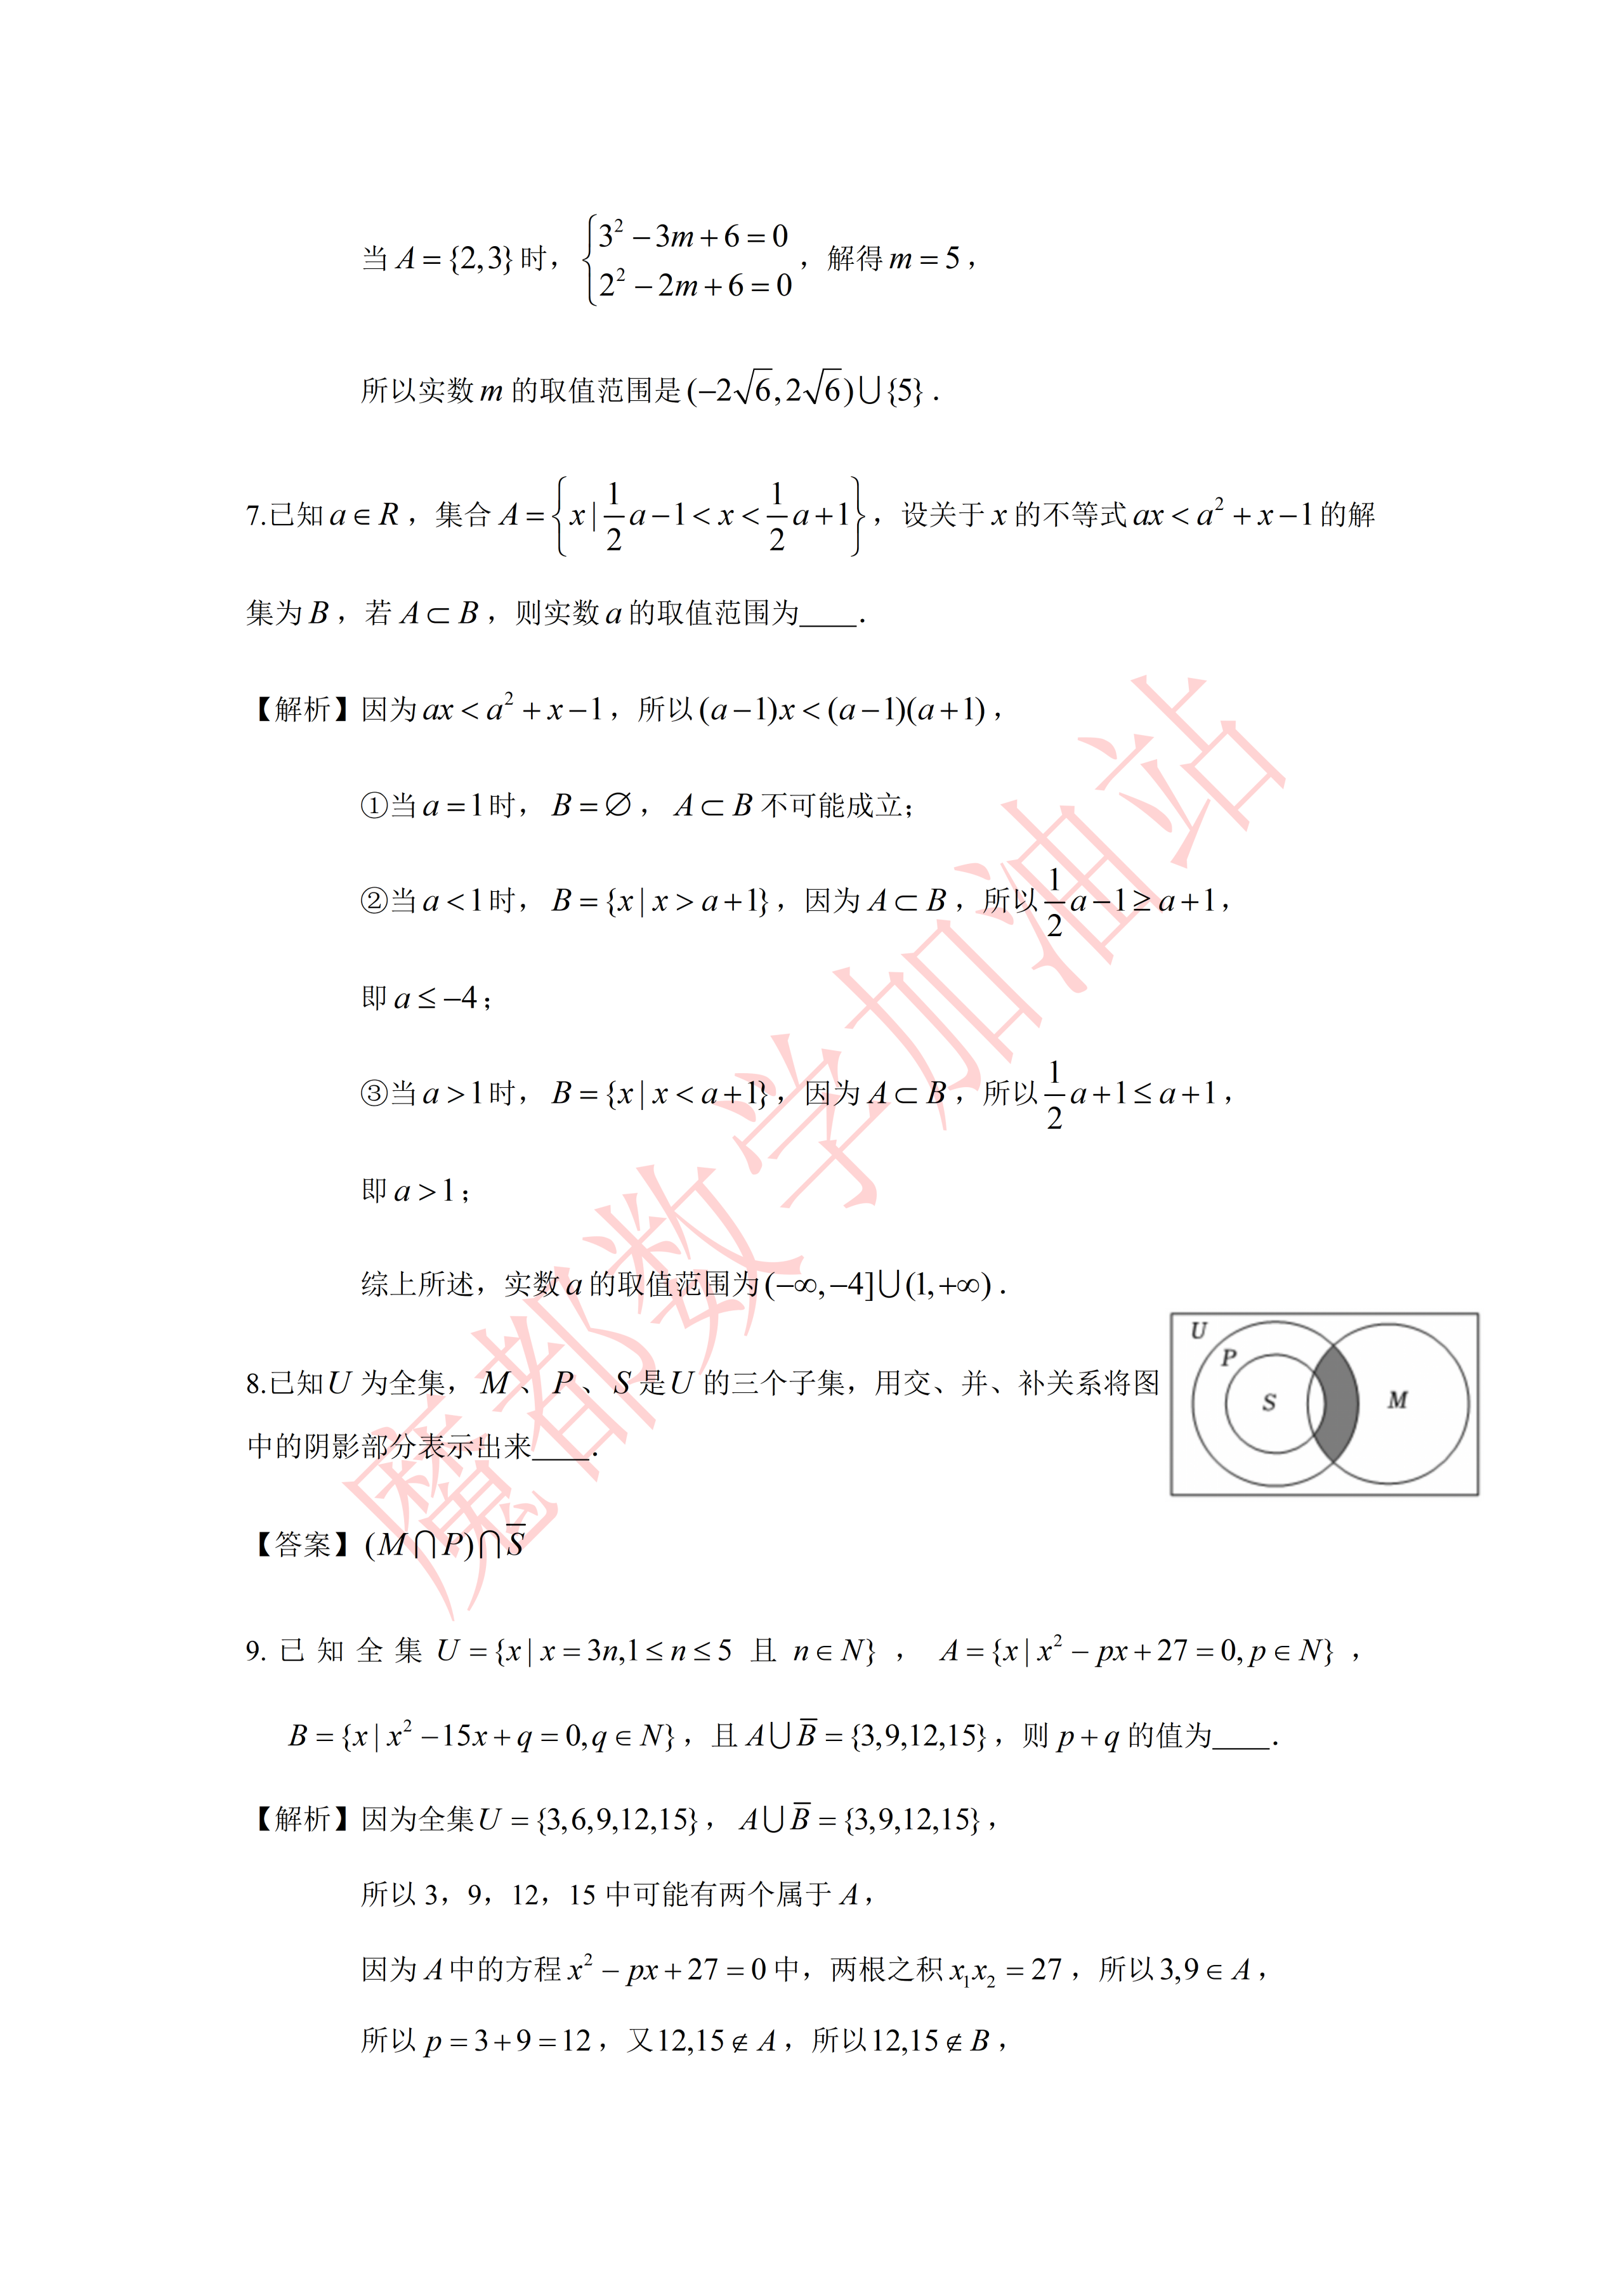
\includegraphics[width=.38\linewidth,trim=1835bp 1255bp 220bp 1565bp,clip]{../原图/高一49_华师大二附中_国庆作业1/02.png}
\end{center}

\ifanswer
\ans{$(M\cap P)\cap\overline S$}
\fi

\item 已知全集 $U=\{x\mid x=3n,1\leqslant n\leqslant5\text{ 且 }n\in\N\}$，$A=\{x\mid x^2-px+27=0,p\in\N\}$，$B=\{x\mid x^2-15x+q=0,q\in\N\}$，且 $A\cup\overline B=\{3,9,12,15\}$，则 $p+q$ 的值为\blankline[4.4em].

\ifanswer
\solbegin
\step{因为全集 $U=\{3,6,9,12,15\}$，$A\cup\overline B=\{3,9,12,15\}$，}
\step{所以 $3$、$9$、$12$、$15$ 中可能有两个属于 $A$，}
\step{因为 $A$ 中的方程 $x^2-px+27=0$ 中，两根之积 $x_1x_2=27$，所以 $3,9\in A$，}
\step{所以 $p=3+9=12$，又 $12,15\notin A$，所以 $12,15\notin B$，}
\step{因为 $B$ 中的方程 $x^2-15x+q=0$ 中，两根之和 $x_3+x_4=15$，所以 $6,9\in B$，}
\step{则 $q=6\times9=54$，所以 $p+q=66$.}
\solend
\fi

\item 已知集合 $A=\{x\mid x^2+(2a-3)x-3a=0,a\in\R,x\in\R\}$，集合 $B=\{x\mid x^2+(a-3)x+a^2-3a=0,a\in\R,x\in\R\}$，若 $A\neq B$，$A\cap B\neq\varnothing$，则 $A\cup B=$\blankline[4.4em].

\ifanswer
\solbegin
\step{设两个集合中的方程的公共解是 $b$，}
\step{由 $b^2+(2a-3)b-3a=b^2+(a-3)b+a^2-3a$，得 $ab=a^2$，}
\step{则 $a=0$ 或 $b=a$，}
\step{当 $a=0$ 时，不合题意，}
\step{当 $b=a$ 时，即两个方程的公共解为 $b=a$，}
\step{将 $b=a$ 代入方程，得 $a^2=2a$，$a=2$，}
\step{所以 $A=\{2,-3\}$，$B=\{-1,2\}$，所以 $A\cup B=\{-1,2,-3\}$.}
\solend
\fi

\item 已知一个有四个数字元素的集合 $S$，$S$ 的所有子集的元素和（空集的元素和认为是 $0$）的总和为 $16192$，则 $S$ 的元素之和等于\blankline[4.4em].

\ifanswer
\solbegin
\step{设 $S=\{a_1,a_2,a_3,a_4\}$，$S$ 的每个元素在所有子集中均出现 $2^3$ 次，}
\step{故 $(a_1+a_2+a_3+a_4)\cdot2^3=16192$，所以 $a_1+a_2+a_3+a_4=2024$，}
\step{故 $S$ 的元素之和等于 $2024$.}
\solend
\fi

\item 设 $P$ 为非空实数集满足：对任意给定的 $x,y\in P$（$x$、$y$ 可以相同），都有 $x+y\in P,x-y\in P,xy\in P$，则称 $P$ 为封闭集．关于封闭集有下列结论：

①集合 $P=\{-2,-1,0,1,2\}$ 为封闭集；

②集合 $P=\{x\mid x=2n,n\in\Z\}$ 为封闭集；

③若集合 $P_1$、$P_2$ 为封闭集，则 $P_1\cup P_2$ 为封闭集；

④若集合 $P$ 为封闭集，则一定有 $0\in P$；

⑤若集合 $P_1$、$P_2$ 为封闭集，则 $P_1\cap P_2$ 为封闭集.

其中正确结论的序号是\blankline[4.4em].

\ifanswer
\solbegin
\step{对于集合 $P=\{-2,-1,0,1,2\}$，取 $x=2$，$y=-2$，则 $x-y=2-(-2)=4\notin P$，}
\step{不满足封闭集的定义，所以①错误.}
\step{对于集合 $P=\{x\mid x=2n,n\in\Z\}$，设 $x=2n_1$，$y=2n_2$，$n_1,n_2\in\Z$.}
\step{$x+y=2n_1+2n_2=2(n_1+n_2)$，因为 $n_1+n_2\in\Z$，所以 $x+y\in P$.}
\step{$x-y=2n_1-2n_2=2(n_1-n_2)$，因为 $n_1-n_2\in\Z$，所以 $x-y\in P$.}
\step{$xy=2n_1\times2n_2=4n_1n_2=2(2n_1n_2)$，因为 $2n_1n_2\in\Z$，所以 $xy\in P$.}
\step{满足封闭集的定义，所以②正确.}
\step{令 $P_1=\{x\mid x=2n,n\in\Z\}$，$P_2=\{x\mid x=3n,n\in\Z\}$，都是封闭集.}
\step{$P_1\cup P_2$ 中，取 $x=2(x\in P_1)$，$y=3(y\in P_2)$，$x+y=5\notin P_1\cup P_2$，}
\step{不满足封闭集的定义，所以③错误.}
\step{因为对任意 $x\in P$，有 $x-x=0\in P$，}
\step{所以若集合 $P$ 为封闭集，则一定有 $0\in P$，所以④正确.}
\step{因为 $P_1$、$P_2$ 为封闭集，设 $x,y\in P_1\cap P_2$，则 $x,y\in P_1$ 且 $x,y\in P_2$.}
\step{因为 $P_1$ 是封闭集，所以 $x+y\in P_1,x-y\in P_1,xy\in P_1$.}
\step{因为 $P_2$ 是封闭集，所以 $x+y\in P_2,x-y\in P_2,xy\in P_2$.}
\step{所以 $x+y\in P_1\cap P_2,x-y\in P_1\cap P_2,xy\in P_1\cap P_2$，满足封闭集的定义，}
\step{所以⑤正确.}
\step{故正确的是②④⑤.}
\solend
\fi

\end{enumerate}

\bigsec{二、选择题}

\begin{enumerate}
\setcounter{enumi}{12}

\item 已知集合 $A=\{1,3,\sqrt m\}$，$B=\{1,m\}$，$B\subseteq A$，则 $m=$\mbox{（\quad）}

\keepwithprev
A. $0$ 或 $\sqrt3$\qquad B. $0$ 或 $3$

C. $1$ 或 $\sqrt3$\qquad D. $1$ 或 $3$

\ifanswer
\solbegin
\step{因为集合 $A=\{1,3,\sqrt m\}$，$B=\{1,m\}$，$B\subseteq A$，所以 $m=3$ 或 $m=\sqrt m$，}
\step{若 $m=3$，$A=\{1,3,\sqrt3\}$，$B=\{1,3\}$，满足 $B\subseteq A$，}
\step{若 $m=\sqrt m$，解得 $m=1$ 或 $m=0$，}
\step{①若 $m=0$，则 $A=\{1,3,0\}$，$B=\{1,0\}$，满足 $B\subseteq A$.}
\step{②若 $m=1$，则 $A$、$B$ 不满足集合中元素的互异性，舍去.}
\step{综上，$m=0$ 或 $m=3$．故选 $B$.}
\solend
\fi

\needvspace{10\baselineskip}

\item 设集合 $A$、$B$、$C$、$D$ 是全集 $X$ 的子集，$A\cap B\neq\varnothing$，$A\cap C\neq\varnothing$，则下列选项中正确的是\mbox{（\quad）}

\keepwithprev
A. 如果 $D\subset B$ 或 $D\subset C$，则 $D\cap A\neq\varnothing$

B. 如果 $D\subset A$，则 $\overline D\cap B\neq\varnothing$，$\overline D\cap C\neq\varnothing$

C. 如果 $A\subset D$，则 $\overline D\cap B=\varnothing$，$\overline D\cap C=\varnothing$

D. 上述各项都不正确

\ifanswer
\solbegin
\step{用韦恩图表示每个选项：}
\begin{center}
% 原图第 5 页解析配图（三联韦恩图）直接裁取（原卷排于选项 C、D 右侧）。
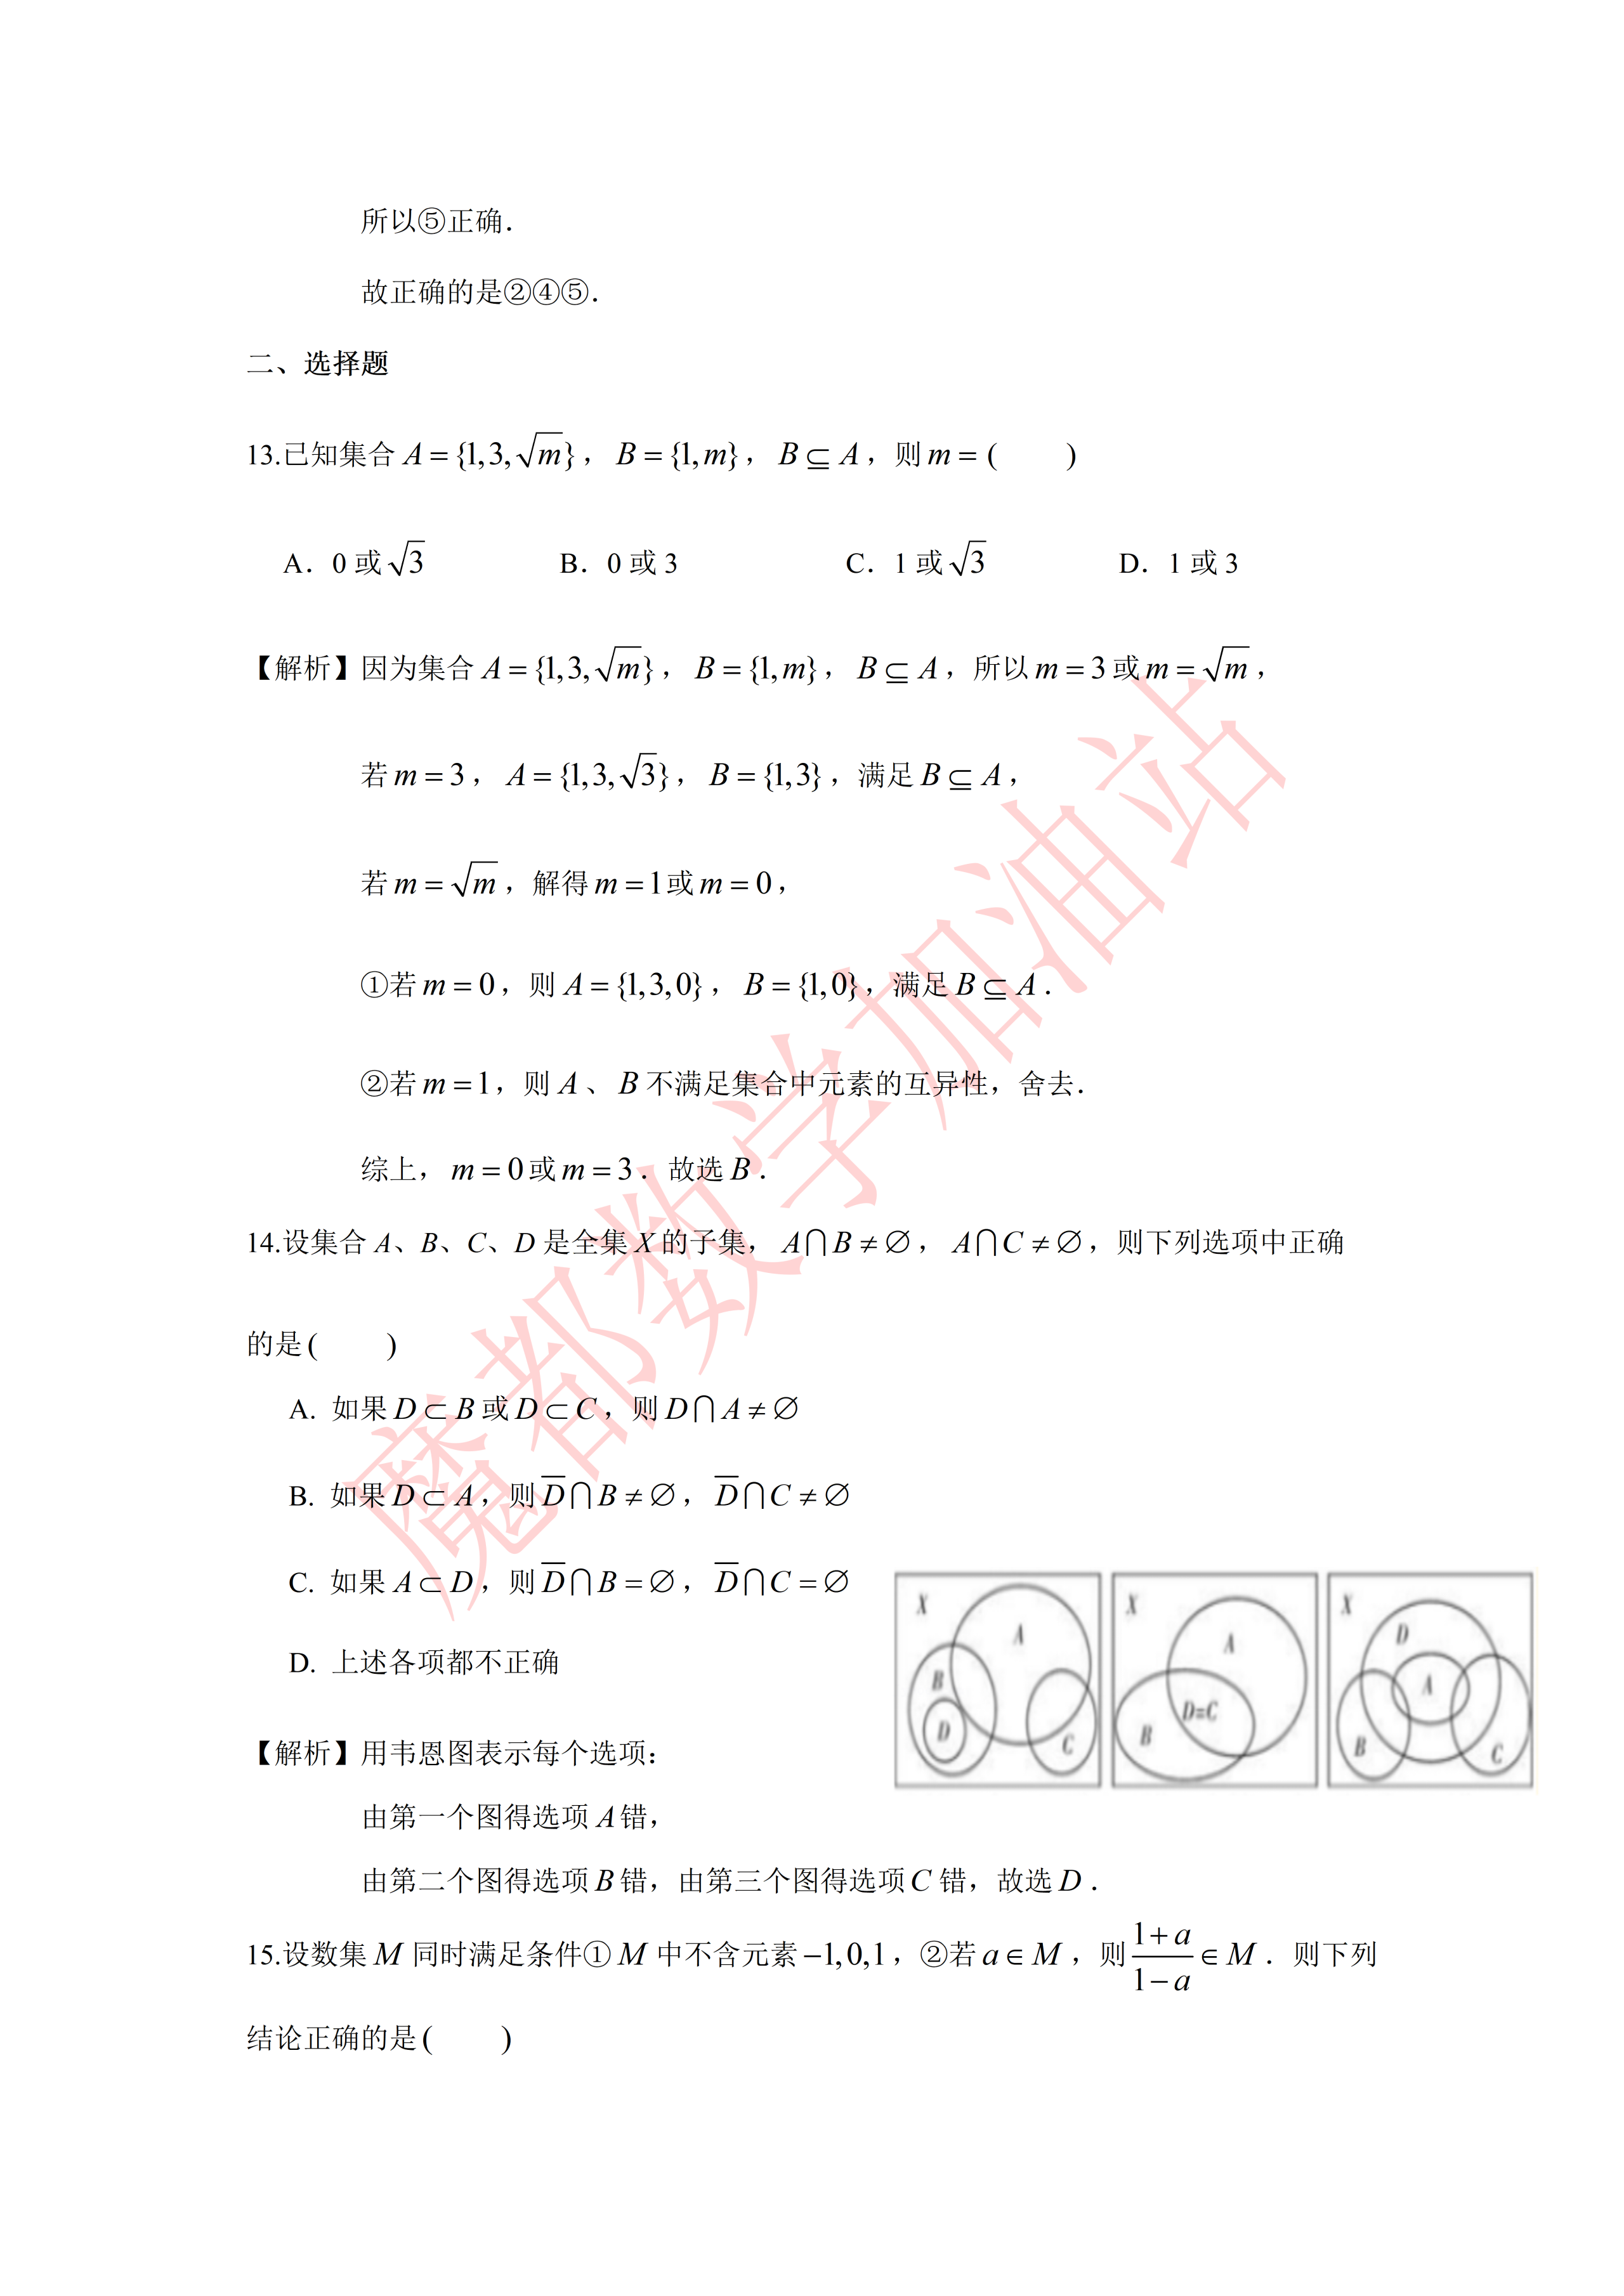
\includegraphics[width=.75\linewidth,trim=1400bp 790bp 135bp 1155bp,clip]{../原图/高一49_华师大二附中_国庆作业1/05.png}
\end{center}
\step{由第一个图得选项 $A$ 错，}
\step{由第二个图得选项 $B$ 错，由第三个图得选项 $C$ 错，故选 $D$.}
\solend
\fi

\item 设数集 $M$ 同时满足条件①$M$ 中不含元素 $-1$、$0$、$1$，②若 $a\in M$，则 $\dfrac{1+a}{1-a}\in M$．则下列结论正确的是\mbox{（\quad）}

\keepwithprev
A. 集合 $M$ 中至多有 $2$ 个元素\qquad B. 集合 $M$ 中至多有 $3$ 个元素

C. 集合 $M$ 中有且仅有 $4$ 个元素\qquad D. 集合 $M$ 中有无穷多个元素

\ifanswer
\solbegin
\step{若集合只含有一个元素，则 $\dfrac{1+a}{1-a}=a$，即 $1+a=a-a^2$，即 $-a^2=1$，不成立.}
\step{当 $a=3$ 时，$\dfrac{1+3}{1-3}=-2\in M$，所以 $\dfrac{1-2}{1+2}=-\dfrac13\in M$，所以 $\dfrac{1-\frac13}{1+\frac13}=\dfrac12\in M$，}
\step{所以 $\dfrac{1+\frac12}{1-\frac12}=3$，开始重复了，所以 $M=\left\{3,-2,-\dfrac13,\dfrac12\right\}$；}
\step{当 $a=2$ 时，$\dfrac{1+2}{1-2}=-3\in M$，所以 $\dfrac{1-3}{1+3}=-\dfrac12\in M$，所以 $\dfrac{1-\frac12}{1+\frac12}=\dfrac13\in M$，}
\step{所以 $\dfrac{1+\frac13}{1-\frac13}=2$，开始重复了，所以 $M=\left\{2,-3,-\dfrac12,-\dfrac13\right\}$，}
\step{此时也只要四个元素；}
\step{当 $a=\dfrac34\in M$，则 $7\in M$，若 $7\in M$，则 $-\dfrac43\in M$，}
\step{若 $-\dfrac43\in M$，则 $-\dfrac17\in M$，若 $-\dfrac17\in M$，有 $\dfrac34\in M$，}
\step{由归纳推理得，集合 $M$ 中有且仅有 $4$ 个元素．故选 $C$.}
\solend
\fi

\item 已知集合 $M=\{x\mid x\in\N,0<x\leqslant15\}$，$A_1$、$A_2$、$A_3$ 满足：①$A_1\cup A_2\cup A_3=M$；②每个集合都恰有 $5$ 个元素．集合 $A_i$（$i=1,2,3$）中最大元素与最小元素之和称为 $A_i$ 的特征数，记为 $X_i$（$i=1,2,3$），则 $X_1+X_2+X_3$ 的值不可能为\mbox{（\quad）}

\keepwithprev
A. $37$\qquad B. $39$\qquad C. $48$\qquad D. $57$

\ifanswer
\solbegin
\step{因为集合 $M=\{x\mid x\in\N,0<x\leqslant15\}=\{1,2,3,\cdots,15\}$，}
\step{又因为集合 $A_1$、$A_2$、$A_3$ 中，每个集合恰有 $5$ 个元素，}
\step{且 $A_1\cup A_2\cup A_3=M$ 有 $15$ 个元素，所以集合 $A_1$、$A_2$、$A_3$ 中没有重复元素，}
\step{因为 $1$ 是集合 $M$ 中数值最小的元素，$15$ 是集合 $M$ 中数值最大的元素，}
\step{所以在 $A_i$ 的特征数构成中，必有 $1$ 和 $15$，不妨设 $1\in A_1$，$15\in A_1$，}
\step{要使 $X_1+X_2+X_3$ 最大，则应该在集合 $A_1$ 中首先放置数值较小的元素，}
\step{即 $A_1=\{1,2,3,4,15\}$，所以 $5$ 与 $14$ 是剩下元素中数值最小或最大的元素，}
\step{同理，不妨设 $5\in A_2$，$14\in A_2$，接着在 $A_2$ 中再次放置数值较小的元素，}
\step{即 $A_2=\{5,6,7,8,14\}$，则 $A_3=\{9,10,11,12,13\}$，}
\step{此时 $X_1+X_2+X_3$ 有最大值为 $1+15+5+14+9+13=57$，}
\step{即 $X_1+X_2+X_3\leqslant57$；}
\step{要使 $X_1+X_2+X_3$ 最小，则在集合 $A_1$ 中首先放置数值较大的元素，}
\step{即 $A_1=\{1,12,13,14,15\}$，所以 $2$ 与 $11$ 是剩下元素中数值最小或最大的元素，}
\step{同理，不妨设 $2\in A_2$，$11\in A_2$，接着在 $A_2$ 中再次放置数值较大的元素，}
\step{即 $A_2=\{2,8,9,10,11\}$，则 $A_3=\{3,4,5,6,7\}$，}
\step{此时 $X_1+X_2+X_3$ 有最小值为 $1+15+2+11+3+7=39$，}
\step{即 $X_1+X_2+X_3\geqslant39$，}
\step{综上，$39\leqslant X_1+X_2+X_3\leqslant57$，故选 $A$.}
\solend
\fi

\end{enumerate}

\bigsec{三、解答题}

\begin{enumerate}
\setcounter{enumi}{16}

\item 已知全集为 $\R$，集合 $A=\{x\mid y=\sqrt{(2+x)(4-x)}\}$，$B=\{x\mid-1<x<m+1\}$.

\begin{enumerate}[label=(\arabic*)]
\item 若 $m=4$，求 $A\cup B$、$\overline A\cap B$；
\item 若 $B\subseteq A$，求实数 $m$ 的取值范围.
\end{enumerate}

\ifanswer
\solbegin
\stepm{(1)}{集合 $A=\{x\mid y=\sqrt{(2+x)(4-x)}\}=\{x\mid-2\leqslant x\leqslant4\}$，}
\step{当 $m=4$ 时，$B=\{x\mid-1<x<5\}$.}
\step{所以 $A\cup B=[-2,5)$，$\overline A=\{x\mid x<-2\text{ 或 }x>4\}$，$\overline A\cap B=(4,5)$.}
\stepm{(2)}{因为 $B\subseteq A$，}
% 原卷如此，照录未改（第 17 题(2)解析两处"当 C=∅／当 C≠∅"应为 B，本卷并无集合 C）
\step{当 $C=\varnothing$ 时，$m\leqslant-2$，$B\subseteq A$ 成立；}
\step{当 $C\neq\varnothing$ 时，$m>-2$，$-1<m+1\leqslant4$，解得 $-2<m\leqslant3$，}
\step{综上，$m\leqslant3$，所以实数 $m$ 的取值范围是 $(-\infty,3]$.}
\solend
\fi

\ansspace[6]

\item 用反证法证明：若 $a$、$b$、$c\in\R$，且 $x=a^2-2b+1$，$y=b^2-2c+1$，$z=c^2-2a+1$，则 $x$、$y$、$z$ 中至少有一个不小于 $0$.

\ifanswer
\solbegin
\step{假设 $x$、$y$、$z$ 均小于 $0$，即 $x=a^2-2b+1<0$①，$y=b^2-2c+1<0$②，}
\step{$z=c^2-2a+1<0$③，①$+$②$+$③得 $x+y+z=(a-1)^2+(b-1)^2+(c-1)^2<0$，}
\step{这与 $(a-1)^2+(b-1)^2+(c-1)^2\geqslant0$ 矛盾，则假设不成立，}
\step{所以 $x$、$y$、$z$ 中至少有一个不小于 $0$，得证.}
\solend
\fi

\ansspace[5]

\item 已知全集为 $\R$，实数 $a$、$b$ 满足 $a\neq b$，集合 $M=\{x\mid x^2-3x-4\leqslant0\}$，集合 $A=\{x\mid(x+a)(x+b)>0\}$，集合 $B=\{x\mid x^2+(a-2)x-2a>0\}$.

\begin{enumerate}[label=(\arabic*)]
\item 若 $\overline A=M$，求 $a$、$b$ 的值；
\item 若 $a>b>-1$，求 $A\cap B$；
\item 若 $a^2+a\in\overline B$，求 $a$ 的取值范围.
\end{enumerate}

\ifanswer
\solbegin
\stepm{(1)}{$M=\{x\mid x^2-3x-4\leqslant0\}=\{x\mid-1\leqslant x\leqslant4\}$，$A=\{x\mid(x+a)(x+b)\leqslant0\}$，}
\step{因为 $\overline A=M$，所以 $a=1$，$b=-4$ 或 $a=-4$，$b=1$.}
\stepm{(2)}{因为 $a>b>-1$，所以 $-a<-b<1$，所以 $A=\{x\mid x<-a\text{ 或 }x>-b\}$，}
\step{因为 $B=\{x\mid x^2+(a-2)x-2a>0\}=\{x\mid x<-a\text{ 或 }x>2\}$，}
\step{所以 $A\cap B=\{x\mid x<-a\text{ 或 }x>2\}$，}
\stepm{(3)}{$\overline B=\{x\mid(x-2)(x+a)\leqslant0\}$，}
% 原卷如此，照录未改（第 19 题(3)此处"a(a-1)((a-2)^2≤0"括号不配对；且由左式展开应为
% a(a-1)(a+2)^2≤0，与下句"解得 a=2 …[0,1]∪{2}"按 (a-2)^2 方自洽，见文件头清单第 2 条）
\step{由 $a^2+a\in\overline B$，得 $(a^2+a-2)(a^2+2a)\leqslant0\Leftrightarrow a(a-1)((a-2)^2\leqslant0$，}
\step{解得 $a=2$ 或 $0\leqslant a\leqslant1$，故 $a$ 的取值范围是 $[0,1]\cup\{2\}$.}
\solend
\fi

\ansspace[7]

\item 设数集 $A$ 由实数构成，若 $x\in A$（$x\neq1$ 且 $x\neq0$），则 $\dfrac{1}{1-x}\in A$.

\begin{enumerate}[label=(\arabic*)]
\item 若 $2\in A$，则 $A$ 中至少还有几个元素；
\item 集合 $A$ 是否为双元素集合？请说明理由；
\item 若 $A$ 中元素个数不超过 $8$ 个，所有元素的和为 $\dfrac{14}{3}$，且 $A$ 中有一个元素的平方等于所有元素的积，求集合 $A$.
\end{enumerate}

\ifanswer
\solbegin
\stepm{(1)}{若 $x\in A$，则 $\dfrac{1}{1-x}\in A$，又 $2\in A$，所以 $\dfrac{1}{1-2}=-1\in A$，}
\step{所以 $\dfrac{1}{1-(-1)}=\dfrac12\in A$，所以 $\dfrac{1}{1-\frac12}=2\in A$，}
% 原卷如此，照录未改（第 20 题(1)解析末句"2 个几个元素"衍一"几个"）
\step{所以 $A$ 中至少还有 $2$ 个几个元素；}
\stepm{(2)}{若 $x\in A$（$x\neq1$ 且 $x\neq0$），则 $\dfrac{1}{1-x}\in A$，}
\step{则 $\dfrac{1}{1-\frac{1}{1-x}}=\dfrac{1-x}{-x}\in A$，则 $\dfrac{1}{1-\frac{1-x}{-x}}=x\in A$}
\step{若 $A$ 为双元素集，则 $x=\dfrac{1}{1-x}$ 或 $x=\dfrac{1-x}{-x}$ 或 $\dfrac{1}{1-x}=\dfrac{1-x}{-x}$，均无解，}
\step{所以 $A$ 不可能为双元素集；}
\stepm{(3)}{由 $x\in A$，$\dfrac{1}{1-x}\in A$，得 $\dfrac{1}{1-\frac{1}{1-x}}=\dfrac{x-1}{x}\in A$，得 $\dfrac{1}{1-\frac{x-1}{x}}=x\in A$，}
\step{所以 $\left\{x,\dfrac{1}{1-x},\dfrac{x-1}{x}\right\}\subseteq A$，而 $x\cdot\dfrac{1}{1-x}\cdot\dfrac{x-1}{x}=-1$，}
\step{$A$ 中元素个数为 $3$ 的倍数，则 $A$ 中元素只有 $6$ 个，}
\step{因为 $A$ 中有一个元素的平方等于所有元素的积，}
\step{不妨设 $x^2=1$，解得 $x=-1$ 或 $x=1$（舍），则 $-1$、$\dfrac12$、$2\in A$，}
\step{所以 $-1+\dfrac12+2+m+\dfrac{1}{1-m}+\dfrac{m-1}{m}=\dfrac{14}{3}$，解得 $m=-\dfrac12$ 或 $m=3$ 或 $m=\dfrac23$，}
\step{所以 $A=\left\{\dfrac12,2,-1,-\dfrac12,3,\dfrac23\right\}$.}
\solend
\fi

\ansspace[9]

% 原卷如此，照录未改（第 21 题题干"21.求已知集合"之"求"字疑衍；"任意两个元素 a_i a_j"
% 疑脱逗号；"|a_i-a_j|≥1/30 则称"之前疑脱标点，见文件头清单第 4 条）
\item 求已知集合 $M=\left\{\dfrac{1}{k}\middle|1\leqslant k\leqslant100\text{ 且 }k\in\N^{*}\right\}$，$A=\{a_1,a_2,\cdots,a_n\}$，其中 $n\in\N^{*}$，且 $n\geqslant2$．若 $A\subseteq\N$，且对集合 $A$ 中的任意两个元素 $a_ia_j$，$i\neq j$ 都有 $|a_i-a_j|\geqslant\dfrac{1}{30}$ 则称集合 $A$ 有性质 $P$.

\begin{enumerate}[label=(\arabic*)]
\item 判断集合 $\left\{\dfrac13,\dfrac14,\dfrac15,\dfrac16,\dfrac17\right\}$ 是否具有性质 $P$；
\item 若集合 $A=\{a_1,a_2,\cdots,a_n\}$ 具有性质 $P$.

①求证：$a_i-a_j$ 的最大值大于等于 $\dfrac{n-1}{30}$；

②求 $A$ 的元素个数 $n$ 的最大值.
\end{enumerate}

\ifanswer
\solbegin
\stepm{(1)}{集合为 $\left\{\dfrac13,\dfrac14,\dfrac15,\dfrac16,\dfrac17\right\}$，又 $\dfrac16-\dfrac17=\dfrac{1}{42}<\dfrac{1}{30}$，所以该集合不具有性质 $P$；}
\stepm{(2)}{①因为集合 $A=\{a_1,a_2,\cdots,a_n\}$ 具有性质 $P$，}
\step{不妨设 $a_1<a_2<a_3<\cdots<a_n$，则 $a_i-a_j\geqslant\dfrac{1}{30}$（$i>j$），}
\step{所以 $a_n-a_1=(a_n-a_{n-1})+(a_{n-1}-a_{n-2})+\cdots+(a_2-a_1)\geqslant\dfrac{n-1}{30}$，}
\step{故 $a_i-a_j$ 的最大值大于等于 $\dfrac{n-1}{30}$；}
% 原卷如此，照录未改（第 21 题(2)②首行"a_2-a_1≥(n-1)/30"：由①同款推理只能得
% a_2-a_1≥1/30，见文件头清单第 5 条）
\step{②$A=\{a_1,a_2,\cdots,a_n\}$，不妨设 $a_1<a_2<a_3<\cdots<a_n$，}
\step{要使 $A$ 的元素个数 $n$ 最大，}
\step{则 $A$ 中的元素满足 $a_n=\dfrac{1}{k}$，$a_{n-1}=\dfrac{1}{k+1}$，$\cdots$，$a_1=\dfrac{1}{k+n-1}$（$k\in\N^{*}$），}
\step{又由①得 $a_2-a_1=\dfrac{1}{k+n-2}-\dfrac{1}{k+n-1}\geqslant\dfrac{n-1}{30}$，}
\step{所以 $(k+n-2)(k+n-1)\leqslant30$，又 $a_n-a_{n-1}=\dfrac{1}{k}-\dfrac{1}{k+1}\geqslant\dfrac{1}{30}$，}
\step{所以 $k(k+1)\leqslant30$，所以 $1\leqslant k\leqslant5$（$k\in\N^{*}$），}
\step{当 $k=5$ 时，由 $(k+n-2)(k+n-1)\leqslant30$，解得 $n\leqslant2$，$n\in\N^{*}$；}
\step{当 $k=4$ 时，由 $(k+n-2)(k+n-1)\leqslant30$，解得 $n\leqslant3$，$n\in\N^{*}$；}
\step{当 $k=3$ 时，由 $(k+n-2)(k+n-1)\leqslant30$，解得 $n\leqslant4$，$n\in\N^{*}$；}
\step{当 $k=2$ 时，由 $(k+n-2)(k+n-1)\leqslant30$，解得 $n\leqslant5$，$n\in\N^{*}$；}
\step{当 $k=1$ 时，由 $(k+n-2)(k+n-1)\leqslant30$，解得 $n\leqslant6$，$n\in\N^{*}$.}
\step{故 $A$ 的元素个数 $n$ 的最大值为 $6$，此时集合 $A=\left\{1,\dfrac12,\dfrac13,\cdots,\dfrac16\right\}$.}
\solend
\fi

\ansspace*[10]

\end{enumerate}

\end{document}
"
%
% 原始材料：微信公众号"魔都数学加油站"文章，作者破晓，连载"27学年高一49"；
% 原文标题"27学年高一49——2026-2027年上海市华师大二附中高一上国庆作业1集合与逻辑、
% 等式与不等式的性质"；页面用 JS 渲染，未见明确发布日期（页内时间戳 ≈ 2026-10-05 21:37）；
% 原文链接：https://mp.weixin.qq.com/s/XxZTOBVQslK5cZm2_BbhOg。
% 正文为 11 张 PNG 页：第 01、03、04、06、07、08、09 页 4762×6735，
% 第 02、05、10、11 页 2560×3620，均按页序读取；粉色斜排"魔都数学加油站"为卷面水印，
% 与公众号页脚一并未录入。全卷 11 页均为试卷页，无二维码/宣传页。
%
% 题号与分节：原文自第 3 题起编，填空题 3—12、选择题 13—16、解答题 17—21，共 19 题。
% 讲评版：原卷每题下直接印【答案】或【解析】——只印【答案】的 3 题（第 3、5、8 题），
% 其余 16 题均只印【解析】；解析行数已逐题按印刷行照录（一条 \step＝原卷一个印刷行）。
%
% 卷首标题：照卷面印作"2026-2027 年华师大二附中高一上国庆作业 1"（公众号标题中的"上海市"
% 卷面没有，本稿照卷面），年份区间按全稿惯例排 en dash；副标题照卷面自印的
% "集合与逻辑单元综合检测"（原卷页首标题行下方即印此行，故不另按模块口径拟名）。
% 副标题依据：全卷 19 题均为集合与常用逻辑用语内容——集合类 15 题（6—17、19—21 中除
% 反证法题外），逻辑/命题类 3 题（第 3 题否定形式、第 4 题充要条件、第 5 题反证法假设），
% 反证法证明 1 题（第 18 题）；全卷无不等式求解题，公众号标题中"等式与不等式的性质"
% 与卷面实际内容不符。
%
% 与原卷的排版差异：
%   ① 原文从第 3 题起，填空题为 3—12、选择题为 13—16、解答题为 17—21，本稿保留原题号；
%   ② 原卷每题下直接印【答案】/【解析】，本稿按全稿惯例置于答案版；只印【解析】的题
%      不另提 \ans{}（照 高一36 口径），只印【答案】的题仅给 \ans{}；
%   ③ 原卷第 8 题韦恩图排在题干右侧、第 14 题三联韦恩图排在选项（C、D）右侧，
%      本稿分别移至题干下方、解析首步之后居中排，均直接裁取原图页（02.png、05.png）；
%   ④ 数集记号原卷排作斜体/加粗 R、N、Z，本稿统一为 \R、\N、\Z、\N^*；
%      填空横线按全稿惯例排为 \blankline[4.4em]。
%
% 原卷笔误/存疑清单（均照录未改，正文中该处有 % 注）：
%   1. 第 17 题(2)解析两处"当 C=∅／当 C≠∅"应为 B（本卷并无集合 C）；
%   2. 第 19 题(3)解析"a(a-1)((a-2)^2≤0"括号不配对（多一枚左括号）；且由
%      (a^2+a-2)(a^2+2a)≤0 展开应为 a(a-1)(a+2)^2≤0，与原卷结论"解得 a=2 …
%      [0,1]∪{2}"恰按 (a-2)^2 自洽——因式分解与原式不符，结论按 (a-2)^2 自洽，均照录；
%   3. 第 20 题(1)解析末句"至少还有 2 个几个元素"衍一"几个"；
%   4. 第 21 题题干"21.求已知集合"之"求"字疑衍；"任意两个元素 a_i a_j"疑脱逗号；
%      "≥1/30 则称"之前疑脱标点；
%   5. 第 21 题(2)②解析"a_2-a_1≥(n-1)/30"：由①同款推理只能得 a_2-a_1≥1/30，
%      原卷如此，照录未改（后续 (k+n-2)(k+n-1)≤30 即按该行推得）。
%
\documentclass[a4paper,11pt]{article}
\usepackage{common}

\begin{document}

\examtitlest[3]{2026--2027 年华师大二附中高一上国庆作业 1}{集合与逻辑单元综合检测}

\bigsec{一、填空题}

\begin{enumerate}
\setcounter{enumi}{2}

\item “若 $x^2-x-2\leqslant0$，则 $-1\leqslant x\leqslant2$”的否定形式为\blankline[4.4em].

\ifanswer
\ans{若 $x^2-x-2>0$，则 $x<-1$ 或 $x>2$}
\fi

\item 已知 $p:|x-3|<5$，$q:1-a<x<2a-3$，且 $p$ 是 $q$ 的充分非必要条件，则实数 $a$ 的取值范围是\blankline[4.4em].

\ifanswer
\solbegin
\step{由 $|x-3|<5$ 得 $-2<x<8$，}
\step{又 $p$ 是 $q$ 的充分不必要条件，所以 $(-2,8)\subset(1-a,2a-3)$，}
\step{即 $\begin{cases}-2\geqslant1-a\\ 8\leqslant2a-3\\ (2a-3)-(1-a)\neq8-(-2)\end{cases}$，解得 $a\geqslant\dfrac{11}{2}$，实数 $a$ 的取值范围是 $\left[\dfrac{11}{2},+\infty\right)$.}
\solend
\fi

\item 用反证法证明命题“设 $a$、$b\in\R$，则方程 $a_1x^2+b_1x+c_1=0$ 与 $a_2x^2+b_2x+c_2=0$ 至少有一个实根”时要做的假设是\blankline[4.4em].

\ifanswer
\ans{假设 $a$、$b\in\R$，方程 $a_1x^2+b_1x+c_1=0$ 与 $a_2x^2+b_2x+c_2=0$ 都没有实根}
\fi

\item 设集合 $A=\{x\mid x^2-mx+6=0,x\in\R\}$，且 $A\cap\{2,3\}=A$，则实数 $m$ 的取值范围是\blankline[4.4em].

\ifanswer
\solbegin
\step{由 $A\cap\{2,3\}=A$，得 $A\subseteq\{2,3\}$，}
\step{当 $A=\varnothing$ 时，$\Delta=m^2-24<0$，解得 $-2\sqrt6<m<2\sqrt6$；}
\step{当 $A=\{2\}$ 时，$\begin{cases}2^2-2m+6=0\\ \Delta=m^2-24=0\end{cases}$，无解；}
\step{当 $A=\{3\}$ 时，$\begin{cases}3^2-3m+6=0\\ \Delta=m^2-24=0\end{cases}$，无解；}
\step{当 $A=\{2,3\}$ 时，$\begin{cases}3^2-3m+6=0\\ 2^2-2m+6=0\end{cases}$，解得 $m=5$，}
\step{所以实数 $m$ 的取值范围是 $(-2\sqrt6,2\sqrt6)\cup\{5\}$.}
\solend
\fi

\item 已知 $a\in\R$，集合 $A=\left\{x\middle|\dfrac12a-1<x<\dfrac12a+1\right\}$，设关于 $x$ 的不等式 $ax<a^2+x-1$ 的解集为 $B$，若 $A\subset B$，则实数 $a$ 的取值范围为\blankline[4.4em].

\ifanswer
\solbegin
\step{因为 $ax<a^2+x-1$，所以 $(a-1)x<(a-1)(a+1)$，}
\step{①当 $a=1$ 时，$B=\varnothing$，$A\subset B$ 不可能成立；}
\step{②当 $a<1$ 时，$B=\{x\mid x>a+1\}$，因为 $A\subset B$，所以 $\dfrac12a-1\geqslant a+1$，}
\step{即 $a\leqslant-4$；}
\step{③当 $a>1$ 时，$B=\{x\mid x<a+1\}$，因为 $A\subset B$，所以 $\dfrac12a+1\leqslant a+1$，}
\step{即 $a>1$；}
\step{综上所述，实数 $a$ 的取值范围为 $(-\infty,-4]\cup(1,+\infty)$.}
\solend
\fi

\needvspace{8\baselineskip}

\item 已知 $U$ 为全集，$M$、$P$、$S$ 是 $U$ 的三个子集，用交、并、补关系将图中的阴影部分表示出来\blankline[4.4em].

\begin{center}
% 原图第 2 页题旁韦恩图直接裁取（原卷排于题干右侧）。
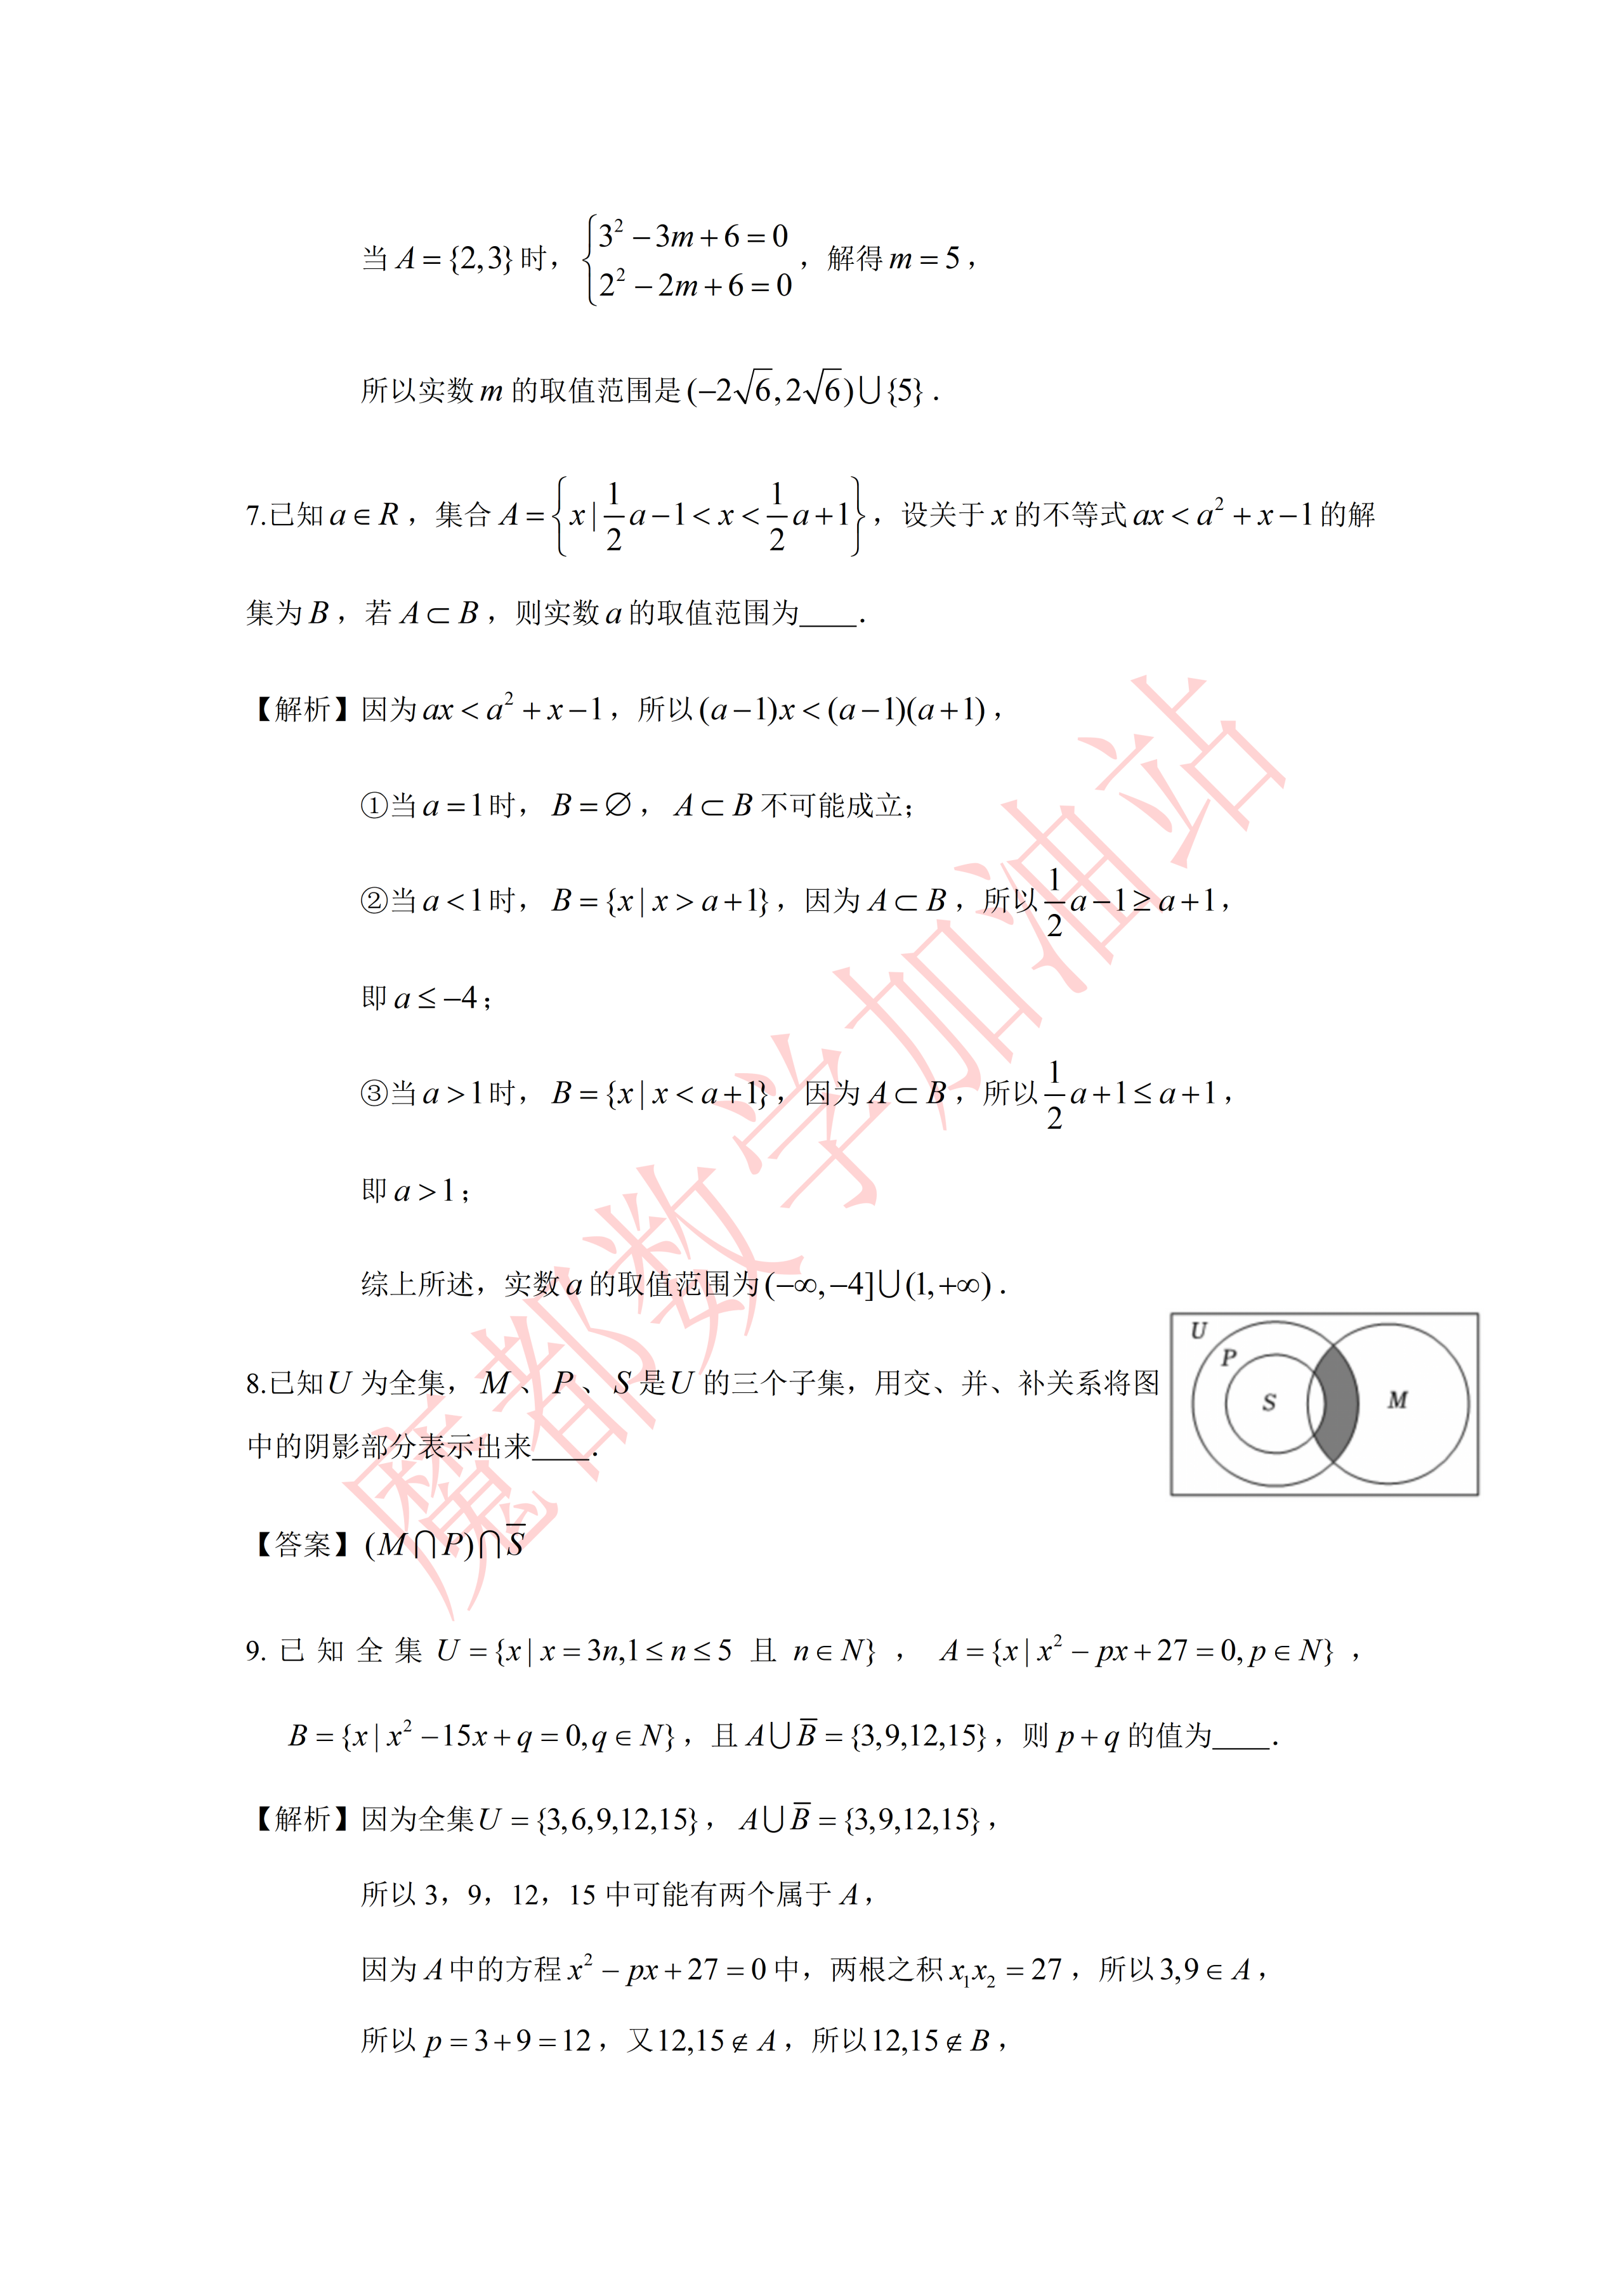
\includegraphics[width=.38\linewidth,trim=1835bp 1255bp 220bp 1565bp,clip]{../原图/高一49_华师大二附中_国庆作业1/02.png}
\end{center}

\ifanswer
\ans{$(M\cap P)\cap\overline S$}
\fi

\item 已知全集 $U=\{x\mid x=3n,1\leqslant n\leqslant5\text{ 且 }n\in\N\}$，$A=\{x\mid x^2-px+27=0,p\in\N\}$，$B=\{x\mid x^2-15x+q=0,q\in\N\}$，且 $A\cup\overline B=\{3,9,12,15\}$，则 $p+q$ 的值为\blankline[4.4em].

\ifanswer
\solbegin
\step{因为全集 $U=\{3,6,9,12,15\}$，$A\cup\overline B=\{3,9,12,15\}$，}
\step{所以 $3$、$9$、$12$、$15$ 中可能有两个属于 $A$，}
\step{因为 $A$ 中的方程 $x^2-px+27=0$ 中，两根之积 $x_1x_2=27$，所以 $3,9\in A$，}
\step{所以 $p=3+9=12$，又 $12,15\notin A$，所以 $12,15\notin B$，}
\step{因为 $B$ 中的方程 $x^2-15x+q=0$ 中，两根之和 $x_3+x_4=15$，所以 $6,9\in B$，}
\step{则 $q=6\times9=54$，所以 $p+q=66$.}
\solend
\fi

\item 已知集合 $A=\{x\mid x^2+(2a-3)x-3a=0,a\in\R,x\in\R\}$，集合 $B=\{x\mid x^2+(a-3)x+a^2-3a=0,a\in\R,x\in\R\}$，若 $A\neq B$，$A\cap B\neq\varnothing$，则 $A\cup B=$\blankline[4.4em].

\ifanswer
\solbegin
\step{设两个集合中的方程的公共解是 $b$，}
\step{由 $b^2+(2a-3)b-3a=b^2+(a-3)b+a^2-3a$，得 $ab=a^2$，}
\step{则 $a=0$ 或 $b=a$，}
\step{当 $a=0$ 时，不合题意，}
\step{当 $b=a$ 时，即两个方程的公共解为 $b=a$，}
\step{将 $b=a$ 代入方程，得 $a^2=2a$，$a=2$，}
\step{所以 $A=\{2,-3\}$，$B=\{-1,2\}$，所以 $A\cup B=\{-1,2,-3\}$.}
\solend
\fi

\item 已知一个有四个数字元素的集合 $S$，$S$ 的所有子集的元素和（空集的元素和认为是 $0$）的总和为 $16192$，则 $S$ 的元素之和等于\blankline[4.4em].

\ifanswer
\solbegin
\step{设 $S=\{a_1,a_2,a_3,a_4\}$，$S$ 的每个元素在所有子集中均出现 $2^3$ 次，}
\step{故 $(a_1+a_2+a_3+a_4)\cdot2^3=16192$，所以 $a_1+a_2+a_3+a_4=2024$，}
\step{故 $S$ 的元素之和等于 $2024$.}
\solend
\fi

\item 设 $P$ 为非空实数集满足：对任意给定的 $x,y\in P$（$x$、$y$ 可以相同），都有 $x+y\in P,x-y\in P,xy\in P$，则称 $P$ 为封闭集．关于封闭集有下列结论：

①集合 $P=\{-2,-1,0,1,2\}$ 为封闭集；

②集合 $P=\{x\mid x=2n,n\in\Z\}$ 为封闭集；

③若集合 $P_1$、$P_2$ 为封闭集，则 $P_1\cup P_2$ 为封闭集；

④若集合 $P$ 为封闭集，则一定有 $0\in P$；

⑤若集合 $P_1$、$P_2$ 为封闭集，则 $P_1\cap P_2$ 为封闭集.

其中正确结论的序号是\blankline[4.4em].

\ifanswer
\solbegin
\step{对于集合 $P=\{-2,-1,0,1,2\}$，取 $x=2$，$y=-2$，则 $x-y=2-(-2)=4\notin P$，}
\step{不满足封闭集的定义，所以①错误.}
\step{对于集合 $P=\{x\mid x=2n,n\in\Z\}$，设 $x=2n_1$，$y=2n_2$，$n_1,n_2\in\Z$.}
\step{$x+y=2n_1+2n_2=2(n_1+n_2)$，因为 $n_1+n_2\in\Z$，所以 $x+y\in P$.}
\step{$x-y=2n_1-2n_2=2(n_1-n_2)$，因为 $n_1-n_2\in\Z$，所以 $x-y\in P$.}
\step{$xy=2n_1\times2n_2=4n_1n_2=2(2n_1n_2)$，因为 $2n_1n_2\in\Z$，所以 $xy\in P$.}
\step{满足封闭集的定义，所以②正确.}
\step{令 $P_1=\{x\mid x=2n,n\in\Z\}$，$P_2=\{x\mid x=3n,n\in\Z\}$，都是封闭集.}
\step{$P_1\cup P_2$ 中，取 $x=2(x\in P_1)$，$y=3(y\in P_2)$，$x+y=5\notin P_1\cup P_2$，}
\step{不满足封闭集的定义，所以③错误.}
\step{因为对任意 $x\in P$，有 $x-x=0\in P$，}
\step{所以若集合 $P$ 为封闭集，则一定有 $0\in P$，所以④正确.}
\step{因为 $P_1$、$P_2$ 为封闭集，设 $x,y\in P_1\cap P_2$，则 $x,y\in P_1$ 且 $x,y\in P_2$.}
\step{因为 $P_1$ 是封闭集，所以 $x+y\in P_1,x-y\in P_1,xy\in P_1$.}
\step{因为 $P_2$ 是封闭集，所以 $x+y\in P_2,x-y\in P_2,xy\in P_2$.}
\step{所以 $x+y\in P_1\cap P_2,x-y\in P_1\cap P_2,xy\in P_1\cap P_2$，满足封闭集的定义，}
\step{所以⑤正确.}
\step{故正确的是②④⑤.}
\solend
\fi

\end{enumerate}

\bigsec{二、选择题}

\begin{enumerate}
\setcounter{enumi}{12}

\item 已知集合 $A=\{1,3,\sqrt m\}$，$B=\{1,m\}$，$B\subseteq A$，则 $m=$\mbox{（\quad）}

\keepwithprev
A. $0$ 或 $\sqrt3$\qquad B. $0$ 或 $3$

C. $1$ 或 $\sqrt3$\qquad D. $1$ 或 $3$

\ifanswer
\solbegin
\step{因为集合 $A=\{1,3,\sqrt m\}$，$B=\{1,m\}$，$B\subseteq A$，所以 $m=3$ 或 $m=\sqrt m$，}
\step{若 $m=3$，$A=\{1,3,\sqrt3\}$，$B=\{1,3\}$，满足 $B\subseteq A$，}
\step{若 $m=\sqrt m$，解得 $m=1$ 或 $m=0$，}
\step{①若 $m=0$，则 $A=\{1,3,0\}$，$B=\{1,0\}$，满足 $B\subseteq A$.}
\step{②若 $m=1$，则 $A$、$B$ 不满足集合中元素的互异性，舍去.}
\step{综上，$m=0$ 或 $m=3$．故选 $B$.}
\solend
\fi

\needvspace{10\baselineskip}

\item 设集合 $A$、$B$、$C$、$D$ 是全集 $X$ 的子集，$A\cap B\neq\varnothing$，$A\cap C\neq\varnothing$，则下列选项中正确的是\mbox{（\quad）}

\keepwithprev
A. 如果 $D\subset B$ 或 $D\subset C$，则 $D\cap A\neq\varnothing$

B. 如果 $D\subset A$，则 $\overline D\cap B\neq\varnothing$，$\overline D\cap C\neq\varnothing$

C. 如果 $A\subset D$，则 $\overline D\cap B=\varnothing$，$\overline D\cap C=\varnothing$

D. 上述各项都不正确

\ifanswer
\solbegin
\step{用韦恩图表示每个选项：}
\begin{center}
% 原图第 5 页解析配图（三联韦恩图）直接裁取（原卷排于选项 C、D 右侧）。
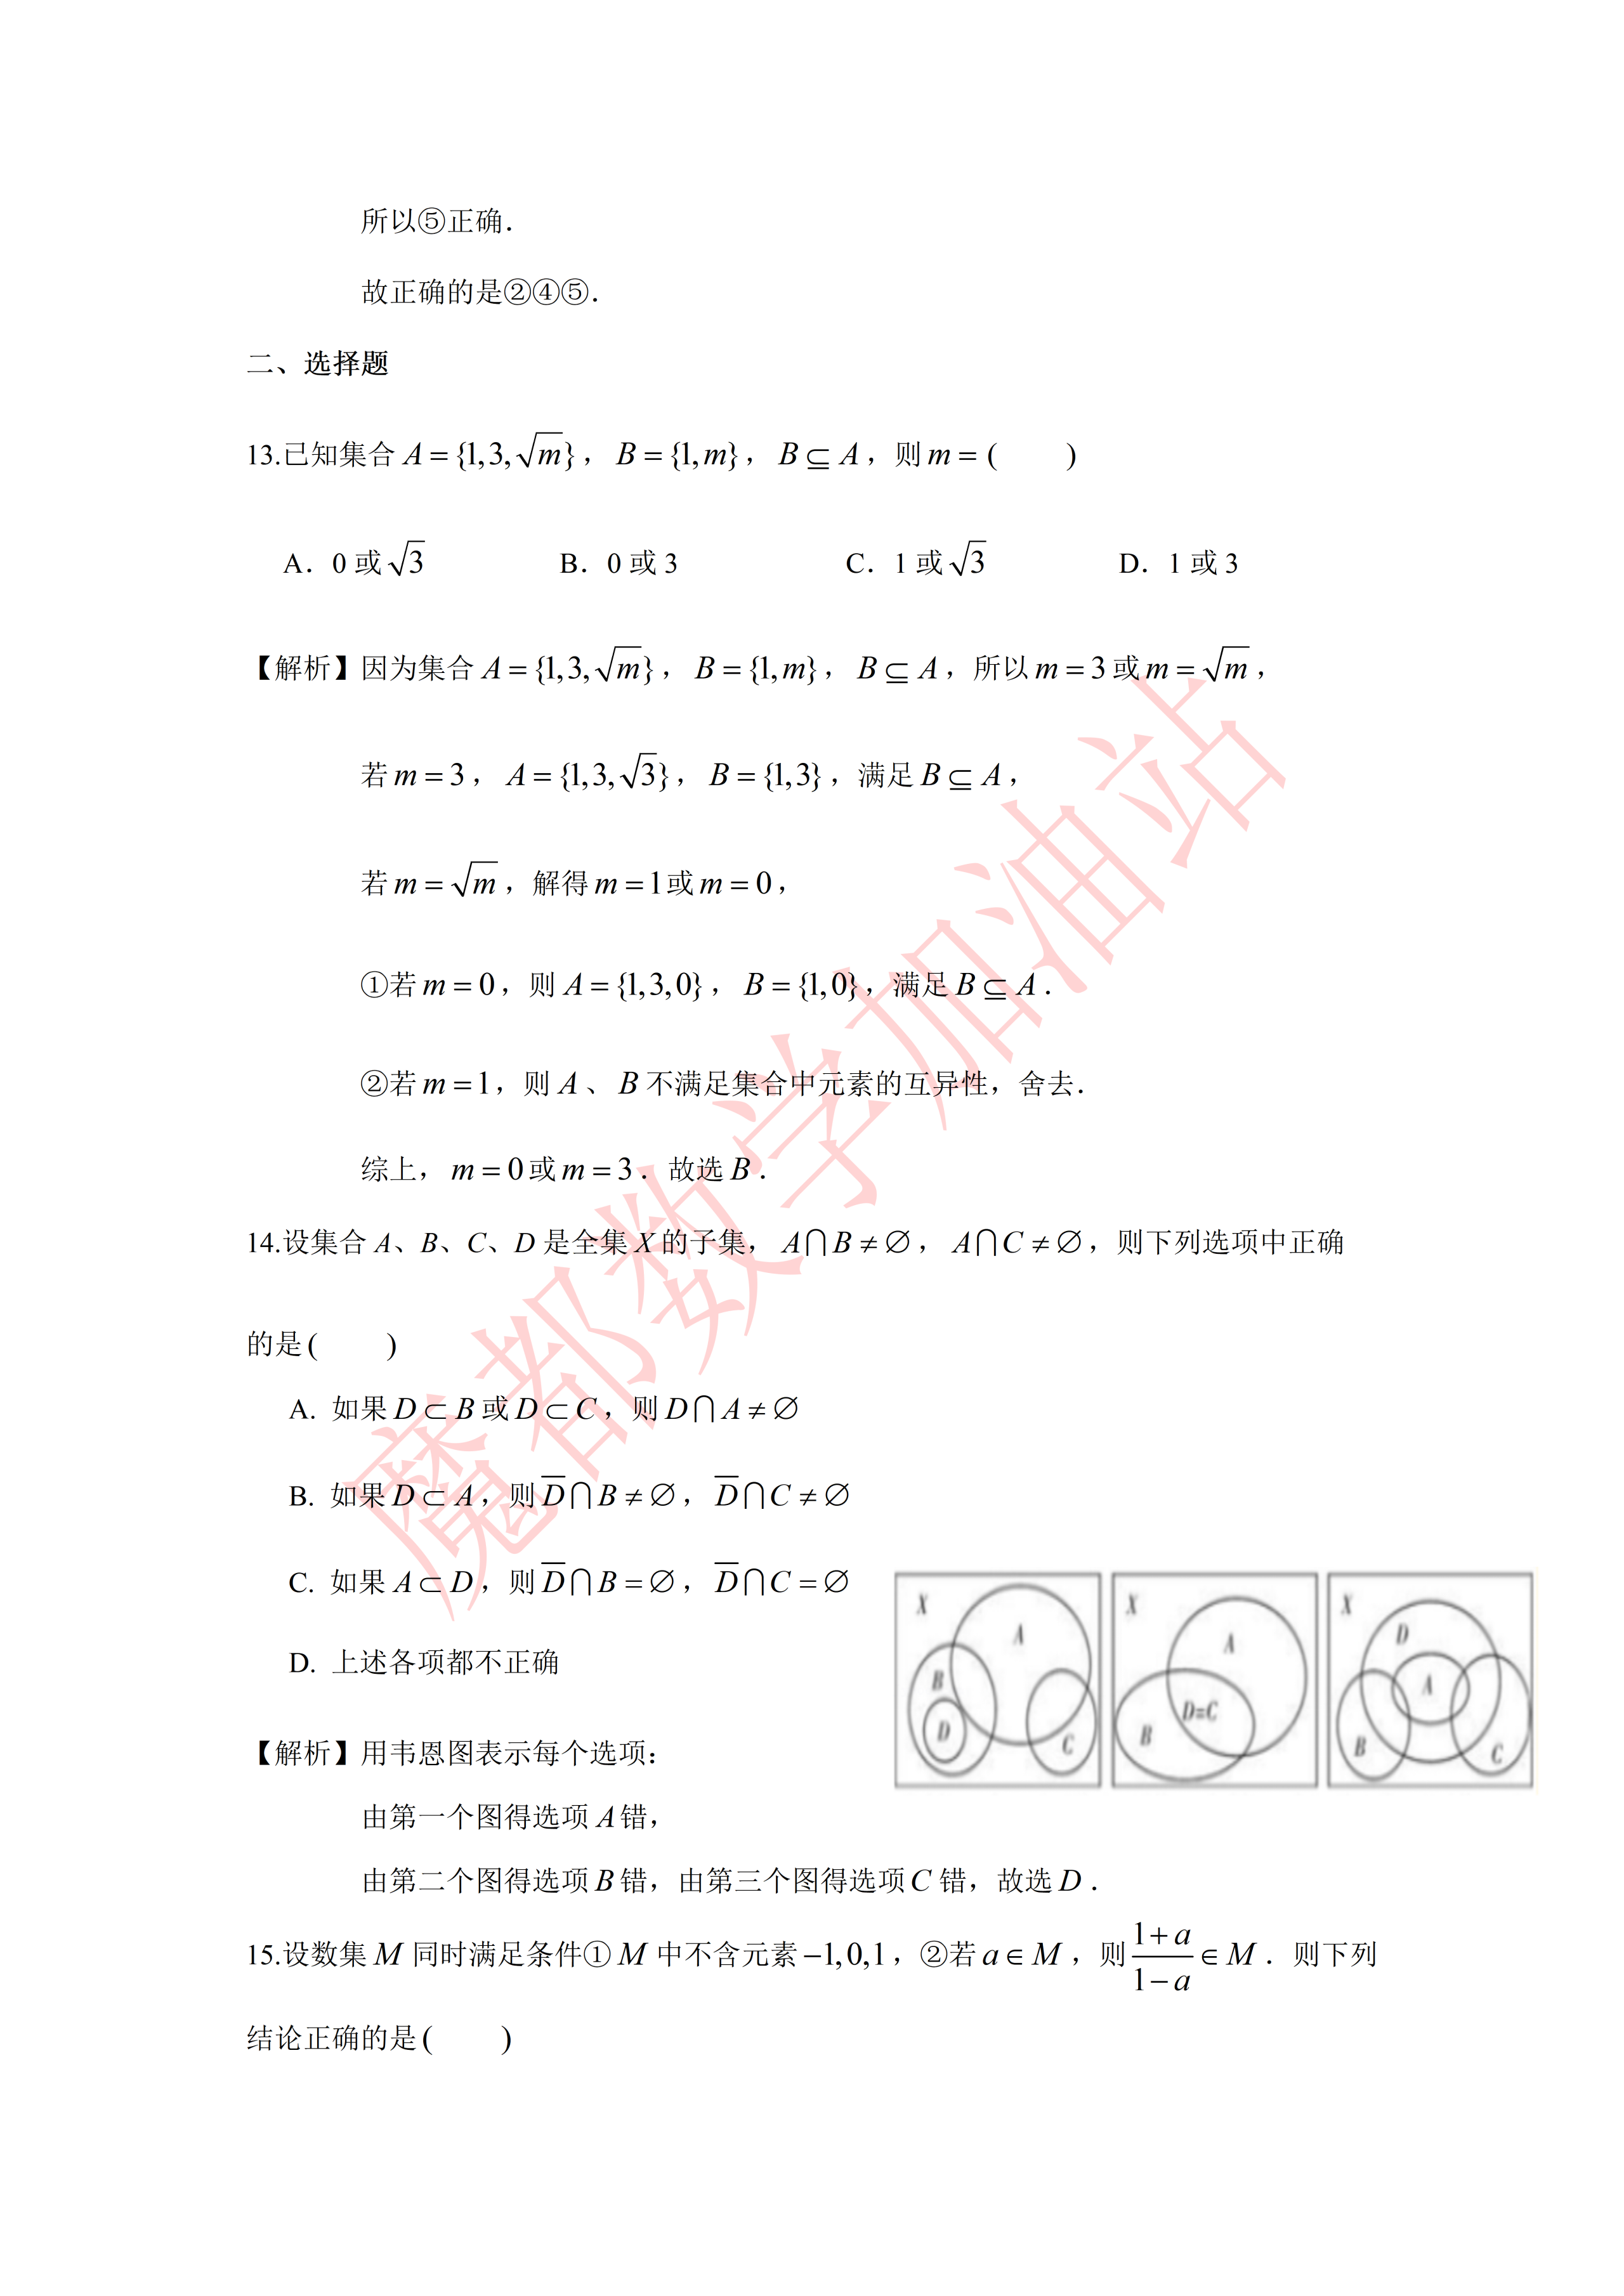
\includegraphics[width=.75\linewidth,trim=1400bp 790bp 135bp 1155bp,clip]{../原图/高一49_华师大二附中_国庆作业1/05.png}
\end{center}
\step{由第一个图得选项 $A$ 错，}
\step{由第二个图得选项 $B$ 错，由第三个图得选项 $C$ 错，故选 $D$.}
\solend
\fi

\item 设数集 $M$ 同时满足条件①$M$ 中不含元素 $-1$、$0$、$1$，②若 $a\in M$，则 $\dfrac{1+a}{1-a}\in M$．则下列结论正确的是\mbox{（\quad）}

\keepwithprev
A. 集合 $M$ 中至多有 $2$ 个元素\qquad B. 集合 $M$ 中至多有 $3$ 个元素

C. 集合 $M$ 中有且仅有 $4$ 个元素\qquad D. 集合 $M$ 中有无穷多个元素

\ifanswer
\solbegin
\step{若集合只含有一个元素，则 $\dfrac{1+a}{1-a}=a$，即 $1+a=a-a^2$，即 $-a^2=1$，不成立.}
\step{当 $a=3$ 时，$\dfrac{1+3}{1-3}=-2\in M$，所以 $\dfrac{1-2}{1+2}=-\dfrac13\in M$，所以 $\dfrac{1-\frac13}{1+\frac13}=\dfrac12\in M$，}
\step{所以 $\dfrac{1+\frac12}{1-\frac12}=3$，开始重复了，所以 $M=\left\{3,-2,-\dfrac13,\dfrac12\right\}$；}
\step{当 $a=2$ 时，$\dfrac{1+2}{1-2}=-3\in M$，所以 $\dfrac{1-3}{1+3}=-\dfrac12\in M$，所以 $\dfrac{1-\frac12}{1+\frac12}=\dfrac13\in M$，}
\step{所以 $\dfrac{1+\frac13}{1-\frac13}=2$，开始重复了，所以 $M=\left\{2,-3,-\dfrac12,-\dfrac13\right\}$，}
\step{此时也只要四个元素；}
\step{当 $a=\dfrac34\in M$，则 $7\in M$，若 $7\in M$，则 $-\dfrac43\in M$，}
\step{若 $-\dfrac43\in M$，则 $-\dfrac17\in M$，若 $-\dfrac17\in M$，有 $\dfrac34\in M$，}
\step{由归纳推理得，集合 $M$ 中有且仅有 $4$ 个元素．故选 $C$.}
\solend
\fi

\item 已知集合 $M=\{x\mid x\in\N,0<x\leqslant15\}$，$A_1$、$A_2$、$A_3$ 满足：①$A_1\cup A_2\cup A_3=M$；②每个集合都恰有 $5$ 个元素．集合 $A_i$（$i=1,2,3$）中最大元素与最小元素之和称为 $A_i$ 的特征数，记为 $X_i$（$i=1,2,3$），则 $X_1+X_2+X_3$ 的值不可能为\mbox{（\quad）}

\keepwithprev
A. $37$\qquad B. $39$\qquad C. $48$\qquad D. $57$

\ifanswer
\solbegin
\step{因为集合 $M=\{x\mid x\in\N,0<x\leqslant15\}=\{1,2,3,\cdots,15\}$，}
\step{又因为集合 $A_1$、$A_2$、$A_3$ 中，每个集合恰有 $5$ 个元素，}
\step{且 $A_1\cup A_2\cup A_3=M$ 有 $15$ 个元素，所以集合 $A_1$、$A_2$、$A_3$ 中没有重复元素，}
\step{因为 $1$ 是集合 $M$ 中数值最小的元素，$15$ 是集合 $M$ 中数值最大的元素，}
\step{所以在 $A_i$ 的特征数构成中，必有 $1$ 和 $15$，不妨设 $1\in A_1$，$15\in A_1$，}
\step{要使 $X_1+X_2+X_3$ 最大，则应该在集合 $A_1$ 中首先放置数值较小的元素，}
\step{即 $A_1=\{1,2,3,4,15\}$，所以 $5$ 与 $14$ 是剩下元素中数值最小或最大的元素，}
\step{同理，不妨设 $5\in A_2$，$14\in A_2$，接着在 $A_2$ 中再次放置数值较小的元素，}
\step{即 $A_2=\{5,6,7,8,14\}$，则 $A_3=\{9,10,11,12,13\}$，}
\step{此时 $X_1+X_2+X_3$ 有最大值为 $1+15+5+14+9+13=57$，}
\step{即 $X_1+X_2+X_3\leqslant57$；}
\step{要使 $X_1+X_2+X_3$ 最小，则在集合 $A_1$ 中首先放置数值较大的元素，}
\step{即 $A_1=\{1,12,13,14,15\}$，所以 $2$ 与 $11$ 是剩下元素中数值最小或最大的元素，}
\step{同理，不妨设 $2\in A_2$，$11\in A_2$，接着在 $A_2$ 中再次放置数值较大的元素，}
\step{即 $A_2=\{2,8,9,10,11\}$，则 $A_3=\{3,4,5,6,7\}$，}
\step{此时 $X_1+X_2+X_3$ 有最小值为 $1+15+2+11+3+7=39$，}
\step{即 $X_1+X_2+X_3\geqslant39$，}
\step{综上，$39\leqslant X_1+X_2+X_3\leqslant57$，故选 $A$.}
\solend
\fi

\end{enumerate}

\bigsec{三、解答题}

\begin{enumerate}
\setcounter{enumi}{16}

\item 已知全集为 $\R$，集合 $A=\{x\mid y=\sqrt{(2+x)(4-x)}\}$，$B=\{x\mid-1<x<m+1\}$.

\begin{enumerate}[label=(\arabic*)]
\item 若 $m=4$，求 $A\cup B$、$\overline A\cap B$；
\item 若 $B\subseteq A$，求实数 $m$ 的取值范围.
\end{enumerate}

\ifanswer
\solbegin
\stepm{(1)}{集合 $A=\{x\mid y=\sqrt{(2+x)(4-x)}\}=\{x\mid-2\leqslant x\leqslant4\}$，}
\step{当 $m=4$ 时，$B=\{x\mid-1<x<5\}$.}
\step{所以 $A\cup B=[-2,5)$，$\overline A=\{x\mid x<-2\text{ 或 }x>4\}$，$\overline A\cap B=(4,5)$.}
\stepm{(2)}{因为 $B\subseteq A$，}
% 原卷如此，照录未改（第 17 题(2)解析两处"当 C=∅／当 C≠∅"应为 B，本卷并无集合 C）
\step{当 $C=\varnothing$ 时，$m\leqslant-2$，$B\subseteq A$ 成立；}
\step{当 $C\neq\varnothing$ 时，$m>-2$，$-1<m+1\leqslant4$，解得 $-2<m\leqslant3$，}
\step{综上，$m\leqslant3$，所以实数 $m$ 的取值范围是 $(-\infty,3]$.}
\solend
\fi

\ansspace[6]

\item 用反证法证明：若 $a$、$b$、$c\in\R$，且 $x=a^2-2b+1$，$y=b^2-2c+1$，$z=c^2-2a+1$，则 $x$、$y$、$z$ 中至少有一个不小于 $0$.

\ifanswer
\solbegin
\step{假设 $x$、$y$、$z$ 均小于 $0$，即 $x=a^2-2b+1<0$①，$y=b^2-2c+1<0$②，}
\step{$z=c^2-2a+1<0$③，①$+$②$+$③得 $x+y+z=(a-1)^2+(b-1)^2+(c-1)^2<0$，}
\step{这与 $(a-1)^2+(b-1)^2+(c-1)^2\geqslant0$ 矛盾，则假设不成立，}
\step{所以 $x$、$y$、$z$ 中至少有一个不小于 $0$，得证.}
\solend
\fi

\ansspace[5]

\item 已知全集为 $\R$，实数 $a$、$b$ 满足 $a\neq b$，集合 $M=\{x\mid x^2-3x-4\leqslant0\}$，集合 $A=\{x\mid(x+a)(x+b)>0\}$，集合 $B=\{x\mid x^2+(a-2)x-2a>0\}$.

\begin{enumerate}[label=(\arabic*)]
\item 若 $\overline A=M$，求 $a$、$b$ 的值；
\item 若 $a>b>-1$，求 $A\cap B$；
\item 若 $a^2+a\in\overline B$，求 $a$ 的取值范围.
\end{enumerate}

\ifanswer
\solbegin
\stepm{(1)}{$M=\{x\mid x^2-3x-4\leqslant0\}=\{x\mid-1\leqslant x\leqslant4\}$，$A=\{x\mid(x+a)(x+b)\leqslant0\}$，}
\step{因为 $\overline A=M$，所以 $a=1$，$b=-4$ 或 $a=-4$，$b=1$.}
\stepm{(2)}{因为 $a>b>-1$，所以 $-a<-b<1$，所以 $A=\{x\mid x<-a\text{ 或 }x>-b\}$，}
\step{因为 $B=\{x\mid x^2+(a-2)x-2a>0\}=\{x\mid x<-a\text{ 或 }x>2\}$，}
\step{所以 $A\cap B=\{x\mid x<-a\text{ 或 }x>2\}$，}
\stepm{(3)}{$\overline B=\{x\mid(x-2)(x+a)\leqslant0\}$，}
% 原卷如此，照录未改（第 19 题(3)此处"a(a-1)((a-2)^2≤0"括号不配对；且由左式展开应为
% a(a-1)(a+2)^2≤0，与下句"解得 a=2 …[0,1]∪{2}"按 (a-2)^2 方自洽，见文件头清单第 2 条）
\step{由 $a^2+a\in\overline B$，得 $(a^2+a-2)(a^2+2a)\leqslant0\Leftrightarrow a(a-1)((a-2)^2\leqslant0$，}
\step{解得 $a=2$ 或 $0\leqslant a\leqslant1$，故 $a$ 的取值范围是 $[0,1]\cup\{2\}$.}
\solend
\fi

\ansspace[7]

\item 设数集 $A$ 由实数构成，若 $x\in A$（$x\neq1$ 且 $x\neq0$），则 $\dfrac{1}{1-x}\in A$.

\begin{enumerate}[label=(\arabic*)]
\item 若 $2\in A$，则 $A$ 中至少还有几个元素；
\item 集合 $A$ 是否为双元素集合？请说明理由；
\item 若 $A$ 中元素个数不超过 $8$ 个，所有元素的和为 $\dfrac{14}{3}$，且 $A$ 中有一个元素的平方等于所有元素的积，求集合 $A$.
\end{enumerate}

\ifanswer
\solbegin
\stepm{(1)}{若 $x\in A$，则 $\dfrac{1}{1-x}\in A$，又 $2\in A$，所以 $\dfrac{1}{1-2}=-1\in A$，}
\step{所以 $\dfrac{1}{1-(-1)}=\dfrac12\in A$，所以 $\dfrac{1}{1-\frac12}=2\in A$，}
% 原卷如此，照录未改（第 20 题(1)解析末句"2 个几个元素"衍一"几个"）
\step{所以 $A$ 中至少还有 $2$ 个几个元素；}
\stepm{(2)}{若 $x\in A$（$x\neq1$ 且 $x\neq0$），则 $\dfrac{1}{1-x}\in A$，}
\step{则 $\dfrac{1}{1-\frac{1}{1-x}}=\dfrac{1-x}{-x}\in A$，则 $\dfrac{1}{1-\frac{1-x}{-x}}=x\in A$}
\step{若 $A$ 为双元素集，则 $x=\dfrac{1}{1-x}$ 或 $x=\dfrac{1-x}{-x}$ 或 $\dfrac{1}{1-x}=\dfrac{1-x}{-x}$，均无解，}
\step{所以 $A$ 不可能为双元素集；}
\stepm{(3)}{由 $x\in A$，$\dfrac{1}{1-x}\in A$，得 $\dfrac{1}{1-\frac{1}{1-x}}=\dfrac{x-1}{x}\in A$，得 $\dfrac{1}{1-\frac{x-1}{x}}=x\in A$，}
\step{所以 $\left\{x,\dfrac{1}{1-x},\dfrac{x-1}{x}\right\}\subseteq A$，而 $x\cdot\dfrac{1}{1-x}\cdot\dfrac{x-1}{x}=-1$，}
\step{$A$ 中元素个数为 $3$ 的倍数，则 $A$ 中元素只有 $6$ 个，}
\step{因为 $A$ 中有一个元素的平方等于所有元素的积，}
\step{不妨设 $x^2=1$，解得 $x=-1$ 或 $x=1$（舍），则 $-1$、$\dfrac12$、$2\in A$，}
\step{所以 $-1+\dfrac12+2+m+\dfrac{1}{1-m}+\dfrac{m-1}{m}=\dfrac{14}{3}$，解得 $m=-\dfrac12$ 或 $m=3$ 或 $m=\dfrac23$，}
\step{所以 $A=\left\{\dfrac12,2,-1,-\dfrac12,3,\dfrac23\right\}$.}
\solend
\fi

\ansspace[9]

% 原卷如此，照录未改（第 21 题题干"21.求已知集合"之"求"字疑衍；"任意两个元素 a_i a_j"
% 疑脱逗号；"|a_i-a_j|≥1/30 则称"之前疑脱标点，见文件头清单第 4 条）
\item 求已知集合 $M=\left\{\dfrac{1}{k}\middle|1\leqslant k\leqslant100\text{ 且 }k\in\N^{*}\right\}$，$A=\{a_1,a_2,\cdots,a_n\}$，其中 $n\in\N^{*}$，且 $n\geqslant2$．若 $A\subseteq\N$，且对集合 $A$ 中的任意两个元素 $a_ia_j$，$i\neq j$ 都有 $|a_i-a_j|\geqslant\dfrac{1}{30}$ 则称集合 $A$ 有性质 $P$.

\begin{enumerate}[label=(\arabic*)]
\item 判断集合 $\left\{\dfrac13,\dfrac14,\dfrac15,\dfrac16,\dfrac17\right\}$ 是否具有性质 $P$；
\item 若集合 $A=\{a_1,a_2,\cdots,a_n\}$ 具有性质 $P$.

①求证：$a_i-a_j$ 的最大值大于等于 $\dfrac{n-1}{30}$；

②求 $A$ 的元素个数 $n$ 的最大值.
\end{enumerate}

\ifanswer
\solbegin
\stepm{(1)}{集合为 $\left\{\dfrac13,\dfrac14,\dfrac15,\dfrac16,\dfrac17\right\}$，又 $\dfrac16-\dfrac17=\dfrac{1}{42}<\dfrac{1}{30}$，所以该集合不具有性质 $P$；}
\stepm{(2)}{①因为集合 $A=\{a_1,a_2,\cdots,a_n\}$ 具有性质 $P$，}
\step{不妨设 $a_1<a_2<a_3<\cdots<a_n$，则 $a_i-a_j\geqslant\dfrac{1}{30}$（$i>j$），}
\step{所以 $a_n-a_1=(a_n-a_{n-1})+(a_{n-1}-a_{n-2})+\cdots+(a_2-a_1)\geqslant\dfrac{n-1}{30}$，}
\step{故 $a_i-a_j$ 的最大值大于等于 $\dfrac{n-1}{30}$；}
% 原卷如此，照录未改（第 21 题(2)②首行"a_2-a_1≥(n-1)/30"：由①同款推理只能得
% a_2-a_1≥1/30，见文件头清单第 5 条）
\step{②$A=\{a_1,a_2,\cdots,a_n\}$，不妨设 $a_1<a_2<a_3<\cdots<a_n$，}
\step{要使 $A$ 的元素个数 $n$ 最大，}
\step{则 $A$ 中的元素满足 $a_n=\dfrac{1}{k}$，$a_{n-1}=\dfrac{1}{k+1}$，$\cdots$，$a_1=\dfrac{1}{k+n-1}$（$k\in\N^{*}$），}
\step{又由①得 $a_2-a_1=\dfrac{1}{k+n-2}-\dfrac{1}{k+n-1}\geqslant\dfrac{n-1}{30}$，}
\step{所以 $(k+n-2)(k+n-1)\leqslant30$，又 $a_n-a_{n-1}=\dfrac{1}{k}-\dfrac{1}{k+1}\geqslant\dfrac{1}{30}$，}
\step{所以 $k(k+1)\leqslant30$，所以 $1\leqslant k\leqslant5$（$k\in\N^{*}$），}
\step{当 $k=5$ 时，由 $(k+n-2)(k+n-1)\leqslant30$，解得 $n\leqslant2$，$n\in\N^{*}$；}
\step{当 $k=4$ 时，由 $(k+n-2)(k+n-1)\leqslant30$，解得 $n\leqslant3$，$n\in\N^{*}$；}
\step{当 $k=3$ 时，由 $(k+n-2)(k+n-1)\leqslant30$，解得 $n\leqslant4$，$n\in\N^{*}$；}
\step{当 $k=2$ 时，由 $(k+n-2)(k+n-1)\leqslant30$，解得 $n\leqslant5$，$n\in\N^{*}$；}
\step{当 $k=1$ 时，由 $(k+n-2)(k+n-1)\leqslant30$，解得 $n\leqslant6$，$n\in\N^{*}$.}
\step{故 $A$ 的元素个数 $n$ 的最大值为 $6$，此时集合 $A=\left\{1,\dfrac12,\dfrac13,\cdots,\dfrac16\right\}$.}
\solend
\fi

\ansspace*[10]

\end{enumerate}

\end{document}
